\documentclass[a4paper,10pt,openany]{book}

\usepackage{glimpse}

\title{M.Sc. Mathematics}
\author{Jacob Antony\\jacobantony987@gmail.com}

\begin{document}

\part{Semester 1}
\chapter{ME010101 Abstract Algebra}
\newcommand{\subgroup}{\le}
\newcommand{\subfield}{\le}
\newcommand{\isomorphism}{\simeq}

%Text Books : \cite{fraleigh}
%Module 1
%Direct products and finitely generated Abelian groups, fundamental theorem, Applications
%Factor groups, Fundamental homomorphism theorem, normal subgroups and inner automorphisms.
%Group action on a set, Isotropy subgroups, Applications of G- sets to counting.
%(Part II – Sections 11, 14, 16 & 17) (25 hours)
%Module 2
%Isomorphism theorems, Sylow theorems , Applications of the Sylow theory.
%(Part VII Sections 34, 36 & 37) (25 hours)
%Module 3
%Fermat’s and Euler Theorems, The field of quotients of an integral domain,
%Rings of polynomials, Factorisation of polynomials over a field.
%(Part IV – Sections 20, 21, 22 & 23) (20 hours)
%Module 4
%Non commutative examples, Homeomorphisms and factor rings, Prime and
%Maximal Ideals
%(Part V – Sections 24, 26 & 27) (20 hours)

%Module 1 - \cite{fraleigh} 11, (13), 14, (15), 16, 17
%Module 2 - \cite{fraleigh} 34, 36, 37
%Module 3 - \cite{fraleigh} 20, 21, 22, 23
%Module 4 - \cite{fraleigh} 24, 26, 27

%Advanced Abstract Algebra
%Module 1 - \cite{fraleigh} 29, 31, 32, 33
%Module 2 - \cite{fraleigh} 45, 46, 47
%Module 3 - \cite{fraleigh} 48, 49, 50
%Module 4 - \cite{fraleigh} 51, 53, 54, 55

%Missing - \cite{fraleigh} 1, 2, 3, 4, 5, 6, 7, 8, 9, 10,
%	12*, 13, 15, 18, 19, 25, 28, 30, 35, 38, 39, 40, 41, 42, 43, 44


\section{Introduction to Abstract Algebra}
%Week 01 Day 01 \S1-10
%\begin{story}
%\paragraph{`Abstract'}
%\footnote{There are many algebras. But, we are interested in the abstract notion 'algebra'.}
%Consider the collection of of all students in a class.
%A person can't be repeated in this collection so you might think this collection is always a set.
%But in this collection, there may be two with name starting with an `S'.
%Thus the collection of first letter of their names can give you the impression that some element is repeated.\\
%
%Thus, though the collection of students is a reality, set is an abstract idea which depends on the details we are interested in.
%And if a particular collection doesn't qualify to be a `set', we can't use set-theoretic results on it.
%(which is, everything below)
%\end{story}

\begin{definition}Set-theoretical foundation of Abstract Algebra
	\begin{itemize}
		\item A \textbf{cartesian product}, $A \times B = \{ (a,b) \ : \ a \in A,\ b \in B \}$%\S0.4
		\item A \textbf{relation} on a set $A$ is a subset of $A \times A$.%\S0.7
		\item A \textbf{function} $f$ from $A$ into $B$,
			$f : A \to B$ is a relation such that \textit{every element of $A$ is related to some unique element of $B$}
			(well defined).%\S0.10
	\end{itemize}
\end{definition}

\begin{definition} Functions :
	A \textbf{binary operation} on a set $A$ is a function $\ast : A \times A \to A$.%\S2.1
	%bi,tri,\dots are numerical prefixes with Latin origin.
	%di is a numerical prefix with Greek origin.
\end{definition}

``A binary operation on a set $A$ gives an algebra on $A$.''%\S1.0
\begin{story}
\paragraph{Abstract Algebra}
	It is the study of algebraic structures.
	We are interested in a few algebraic structures :
	\begin{enumerate*}
		\item Group
		\item Ring
		\item Integral Domain
		\item Field
	\end{enumerate*}
\end{story}

\begin{definition}
	A \textbf{binary algebraic structure} $<\!G,\ast\!>$ is a set $G$ together with a binary operation $\ast$.
\end{definition}

\begin{definition}[Group]
	A set $G$, closed under a binary relation $\ast$ satisfying the following three axioms -G1, G2, \& G3 is a group.%\S4.1
\begin{enumerate}[label=G\arabic*]
	\item Associativity \\
		For any three elements $a,b,c \in G,\ a \ast (b \ast c) = (a \ast b) \ast c$.
	\item Identity element\\
		There exists a unique element $e \in G$ such that $a \ast e = a = e \ast a$ for any element $a \in G$.
	\item Inverse elements\\
		For any element $a \in G$ there exists a unique element $a^{-1}$ such that $a \ast a^{-1} = e = a^{-1} \ast a$.
\end{enumerate}
\end{definition}

\begin{definition}Group terminologies :
	\begin{itemize}
		\item A group is \textbf{abelian} if the binary operation is commutative. $a \ast b = b \ast a$%\S4.3
		\item The \textbf{order} of a group $G,\ast$ is the number of elements in $G$.%\S5.3
	\end{itemize}
\end{definition}

\begin{definition}
	$\mathbb{Z}_n = \{ 0, 1, 2, \cdots, n-1 \}$
\end{definition}

\begin{remark}
	Consider $3,4 \in \mathbb{Z}_5$,
	$3 \ast 4 = 2 = 4 \ast 3$ since $7 \cong 2 \pmod 5$.
	$<\!\mathbb{Z}_5,+_5\!>$ is an abelian group of order 5.
\end{remark}

\begin{definition} Homomorphism \& Isomorphism
	\begin{itemize}
		\item A function $\phi : A \to B$ is a \textbf{homomorphism} if for any two elements $x,y \in A$, $\phi (xy) = \phi(x)\phi(y)$%\S3.7
		\item A function $\phi : A \to B$ is an \textbf{isomorphism} if $\phi$ is a bijective, homomorphism.
			If two binary structures  are isomorphic, then they have the same (algebraic) structure.%\S3.7
	\end{itemize}
\end{definition}

\begin{definition} Subgroup
	\begin{itemize}
		\item A subset $H$ of a group $<\! G,\ast\! >$ is a \textbf{subgroup} of $G$ if $H$ is group with the same binary operation $\ast$.
			And is denoted by $H \subgroup G$.%\S5.4
		\item $G$ is the \textbf{improper} subgroup of $G$ and every other subgroup is \textbf{proper}.S5.5
		\item $\{e\}$ is the \textbf{trivial} subgroup of $G$ and every other subgroup is \textbf{non-trivial}.%\S5.5
		\item The \textbf{subgroup generated by} $g \in G$ is the subgroup $\{ g^n : n \in \mathbb{Z} \}$.%\S5.19
		\item The \textbf{order} of an element $g$ is order of the subgroup generated by $g$.%\S5.19
		\item An element $g \in G$ is a \textbf{generator} of $G$ if $g$ generates $G$.%\S5.19
		\item A group is \textbf{cyclic} if it has a generator.%\S5.19
	\end{itemize}
\end{definition}

\begin{remark}
	Cyclic Groups :
	\begin{itemize}
		\item Cyclic groups are abelian.%\S6.1
		\item Subgroups of cyclic groups are cyclic.%\S6.6
	\end{itemize}
\end{remark}

\subsection{Some Proof Techniques}
\paragraph{Equality of two Sets}
$A = B \iff A \subset B$ and $B \subset A$\\
If $x \in A \implies x \in B$, then $A \subset B$
\paragraph{Uniqueness}
	Suppose there are two elements that qualify our conditions.
	We show (using the conditions) that they are the same, that is, unique.

	For example, $3 + a = \pi$.
	Suppose $a = x,y$.
	Then $3 + x = 3 + y \implies x = y$, provided that the values of $a$ comes from a set in which left cancelation law can be applied.
	Then $a$ is unique.

	Remember : We usually don't care to show what this unique element is.
	It may be also be the case that there is no such element, that is, proof of uniqueness doesn't imply existence.

\paragraph{Existence}
	There are constructive and non-constructive proofs for existence problems.
	Suppose we want to prove that $a\ast b$ has an inverse element.
	We know that $a,b$ has inverse elements $a^{-1},b^{-1}$.
	From those elements, we construct an element $b^{-1} \ast a^{-1}$ which is an inverse of $a \ast b$ by construction.

	And we may also prove existence without actually giving an object.
	Suppose we want to prove that $x^y \in \mathbb{Q}$ for some irrational numbers $x$ and $y$.
	We know that $\sqrt{2} \notin \mathbb{Q}$.
	Then, $\sqrt{2}^{\sqrt{2}}$ is either rational or irrational.
	Suppose it is irrational, then $\left(\sqrt{2}^{\sqrt{2}}\right)^{\sqrt{2}} = 2$ is rational.
	Thus the proof is complete, but we are yet to know whether $\sqrt{2}^{\sqrt{2}}$ is an irrational or rational.

%\pagebreak

%Week 01 Day 02 \S11.1-11
\section{Direct Products and Finitely Generated Abelian Groups}
\begin{definition}[Cartesian product of sets]
	Let $S_1,\ S_2, \cdots,\ S_n$ be a sets.
	Their cartesian product,
	\begin{equation}
		S_1 \times S_2 \times \cdots \times S_n = \prod_{i = 1}^n S_n = \{ (a_1,a_2,\cdots,a_n) :  a_i \in S_i \} 
	\end{equation}
	For example, $ \{A,B,C\} \times \{ 1,2 \} = \{ (A,1),(A,2),(B,1),(B,2),(C,1),(C,2) \}$.
\end{definition}

\begin{question}
	How many elements in $\mathbb{Z}_3 \times \mathbb{Z}_{10} \times \mathbb{Z}_9$ ?
\end{question}

\begin{theorem}[Direct product of Groups]
	Let $G_1,\ G_2,\ \cdots,\ G_n$ be groups.
	Then their cartesian product is a group with the binary operation $\ast$,
	\begin{equation}
		(a_1,\ a_2,\ \cdots,\ a_n) \ast (b_1,\ b_2,\ \cdots,\ b_n) = (a_1 \ast b_1,\ a_2 \ast b_2,\ \cdots,\ a_n \ast b_n)
	\end{equation}
	where the binary operation in  $a_i \ast b_i$ is the binary operation of the group $G_i$.
\end{theorem}
\begin{proof}
	$\prod\limits_{i = 1}^n G_i$ is a group if it satisfies the group axioms.
	\begin{enumerate}[label=G\arabic*]
		\item Associativity
			\begin{align*}
				(a_1,\ a_2,\ & \cdots,\ a_n) \big( (b_1,\ b_2,\ \cdots,\ b_n)(c_1,\ c_2,\ \cdots,\ c_n) \big) \\
				= & (a_1,\ a_2,\ \cdots,\ a_n)(b_1c_1,\ b_2c_2,\ \cdots,\ b_nc_n) \\
				= & \big( a_1(b_1c_1),\ a_2(b_2c_2),\ \cdots,\ a_n(b_nc_n) \big) \\
				= & \big( (a_1 b_1)c_1,\ (a_2b_2)c_2,\ \cdots,\ (a_nb_n )c_n \big) \\
				= &  (a_1b_1,\ a_2b_2,\ \cdots,\ a_nb_n)(c_1,\ c_2,\ \cdots,\ c_n) \\
				= & \big( (a_1,\ a_2,\ \cdots,\ a_n)(b_1,\ b_2,\ \cdots,\ b_n) \big)(c_1,\ c_2,\ \cdots,\ c_n)
			\end{align*}
		\item Existence of a unique identity element in $\prod\limits_{i = 1}^n G_i$\\
			Let $e_i$ be the identity element in $G_i$.
			Then $(e_1,\ e_2,\ \cdots,\ e_n)$ is the identity element in $\prod\limits_{i = 1}^n G_i$.
			\begin{align*}
				(a_1,\ a_2,\ \cdots,\ a_n)&(e_1,\ e_2,\ \cdots, e_n) \\
				& = (a_1e_1,\ a_2e_2,\ \cdots,\ a_ne_n) \\
				& = (a_1,\ a_2,\ \cdots,\ a_n)
			\end{align*}
		\item Existence of unique inverse element for each element in $\prod\limits_{i = 1}^n G_i$\\
			Let $(a_1,\ a_2,\ \cdots, a_n)$ be in $\prod\limits_{i = 1}^n G_i$.
			Then it has the inverse element $( a_1^{-1},\ a_2^{-1},\ \cdots,\ a_n^{-1} )$ in $\prod\limits_{i = 1}^n G_i$.
			\begin{align*}
				(a_1,\ a_2,\ \cdots a_n)&(a_1^{-1},\ a_2^{-1},\ \cdots, a_n^{-1}) \\
				& = (a_1a_1^{-1},\ a_2a_2^{-1},\ \cdots,\ a_na_n^{-1}) \\
				& = (e_1,\ e_2,\ \cdots,\ e_n)
			\end{align*}
	\end{enumerate}
\end{proof}

\begin{remark}
	We usually write $ab$ instead of $a \ast b$ and relevent binary operations are used in different contexts.
	Student should be able to recongnise the difference from the context.
\end{remark}

\begin{remark}
	$\mathbb{Z}_n = \{ 0,1,\cdots,(n-1) \}$ is a group with $+_n$.
	(addition modulo $n$)

	For example, Consider $(1,2) \in \mathbb{Z}_2 \times \mathbb{Z}_3$.
	We have, $(1,2) + (1,2) = (0,1)$ since $1 +_2 1=0$ and $2 +_3 2 = 1$.
\end{remark}

\begin{definition}
	Suppose all the groups $G_i$ are abelian.
	Then $\prod\limits_{i = 1}^n G_i$ is the direct sum of the groups $G_i$.
	And is represented by $\oplus_{i = 1}^n G_i$.
\end{definition}

\begin{theorem}
	$\mathbb{Z}_m \times \mathbb{Z}_n$ is cyclic and is isomorphic to $\mathbb{Z}_{mn}$ if and only if $m$ and $n$ are relatively prime.
\end{theorem}
\begin{proof}
	Sufficient part :
	Consider the cyclic subgroup\footnote{$(1,1) \in Z_m \times Z_n$.
	The cyclic group generated by $(1,1)$ has all its elements in $Z_m \times Z_n$.
	And therefore, it is a subgroup of $Z_m \times Z_n$} $H$ generated by $(1,1) \in \mathbb{Z}_m \times \mathbb{Z}_n$.
	It is enough to prove that the order of this cyclic subgroup $H$ is $mn$.
	The order of $H$ is the smallest power of $(1,1)$ that gives the identity $(0,0)$.
	The first component gives $0$ for multiples of $m$.
	And the second component gives $0$ for multiples of $n$.
	Since $m,n$ are relatively prime, $mn$ is the smallest power of $(1,1)$ that will give $(0,0)$.
	Thus $\mathbb{Z}_m \times \mathbb{Z}_n = H$ and is cyclic.
	\begin{important} Every cyclic group of order $mn$ is isomorphic to $\mathbb{Z}_{mn}$. Therefore, $\mathbb{Z}_m \times \mathbb{Z}_n \approx \mathbb{Z}_{mn}$.\end{important}

	Necessary part :
	Suppose $\gcd(m,n) = d > 1$.
	Then $mn/d$ is the smallest integer divisible by both $m$ and $n$.
	Consider $(r,s) \in \mathbb{Z}_m \times \mathbb{Z}_n$.
	$r$ gives $0$ in $mn/d$ since it is a multiple of $m$.
	Similarly, $s$ gives $0$ in $mn/d$ since it is a multiple of $n$.
	Thus, $\frac{mn}{d} (r,s) = (0,0)$.
	And the cyclic group generated by any element of $\mathbb{Z}_m \times \mathbb{Z}_n$ is a proper subgroup.
	Therefore $\mathbb{Z}_m \times \mathbb{Z}_n$ has no generators and it is not cyclic.
\end{proof}

\begin{corollary}
	$\prod\limits_{i = 1}^n \mathbb{Z}_{m_i}$ is cyclic and is isomorphic to $Z_{m_1m_2\cdots m_n}$ if and only if any two of the numbers $m_i$ are relatively prime.
\end{corollary}

\begin{question}
	Prove : For any non-negative integer $n$, there exists a cyclic group of order $n$, which is unique upto isomorphism.
\end{question}

\begin{theorem}
	Let $(a_1,\ a_2,\ \cdots,\ a_n) \in \prod\limits_{i = 1}^n G_i$. And $a_i$ are of finite order $r_i$ in $G_i$. Then the order of $\prod\limits_{i = 1}^n G_i$ is the least common multiple of $r_i$s.
\end{theorem}
\begin{proof}
	Least common multiple of $r_i$s is the smallest positive integer $d$ which is a multiple of all $r_i$s.
	For each $i$, the $r_i$th multiple of $a_i$ gives $0$ (identity).
	Thus, the order of the cyclic subgroup generated by $(a_1,\ a_2,\ \cdots,\ a_n)$ is the least common multiple of all the $r_i$s.
\end{proof}
\begin{remark}
	Consider $(3,6,12,16) \in \mathbb{Z}_4 \times \mathbb{Z}_{12} \times \mathbb{Z}_{20} \times \mathbb{Z}_{24}$.
	Order of $3 \in \mathbb{Z}_4$ is ${4}/{\gcd(3,4)} = 4$ ie, $<3> = \{ 3,2,1,0 \}$\\
	Order of $6 \in \mathbb{Z}_{12}$ is ${12}/{\gcd(6,12)} = 2$ ie, $<6> = \{ 6,0 \}$\\
	Order of $12 \in \mathbb{Z}_{20}$ is ${20}/{\gcd(12,20)} = 5$ ie, $<12> = \{ 12,4,16,8,0 \}$\\
	Order of $16 \in \mathbb{Z}_{24}$ is ${24}/{\gcd(16,24)} = 3$ ie, $<16> = \{ 16,8,0 \}$\\
	Order of $(3,6,12,16)$ is $lcm(4,2,5,3) = 2^2\ 3\ 5 = 60$.
\end{remark}

\begin{remark}
	Define $\overline{G_i} = \{ (e_1,\ e_2,\ \cdots,\ e_{i-1},\ a_i,\ e_{i+1},\ \cdots,\ e_n) : a_i \in G_i\}$.
	Then $G_i \approx \overline{G_i}$.
	And $\prod\limits_{i=1}^n G_i$ is the internal direct product of $\overline{G_i}$s.

	For example, $\mathbb{Z}_2 \times \mathbb{Z}_3 \approx \left( \mathbb{Z}_2 \times \{ 0 \} \right) \otimes \left( \{ 0 \} \times \mathbb{Z}_3 \right)$
\end{remark}

\begin{question}
	Internal direct product form of $\mathbb{Z}_{12} \times \mathbb{Z}_{60} \times \mathbb{Z}_{24}$ ?
\end{question}
%\pagebreak

%Week 01 Day 03 \S11.11-17
\section{Fundamental Theorem}
\begin{definition}
	A group $G$ is \textbf{finitely generated} if $G$ has a finite subset that generates $G$.
%	For example, $\{ 1,\rho^2,\mu,\mu\rho^2 \}$ is a finitely generated subgroup of $D_8$.
\end{definition}

\begin{theorem}[fundamental theorem of finitely generated abelian groups]
	Every finitely generated abelian group $G$ is isomorphic to a direct product of cyclic groups in the form
	\begin{equation}
		\mathbb{Z}_{{p_1}^{r_1}} \times\mathbb{Z}_{{p_2}^{r_2}} \times \cdots \times \mathbb{Z}_{{p_n}^{r_n}} \times \mathbb{Z} \times \mathbb{Z} \times \cdots \times \mathbb{Z}
	\end{equation}
	where $p_i$ are primes, not necessarily distict and $r_i$ are positive integers.
	The direct product is unique, except for the possible rearrangement of the factors.
\end{theorem}
\begin{proof}
	---proof is omitted---
\end{proof}

For example, $ G = \mathbb{Z}_{20} \times \mathbb{Z} \times \mathbb{Z}_{15} \times \mathbb{Z} \approx \mathbb{Z}_{2^2} \times \mathbb{Z}_3 \times \mathbb{Z}_5 \times \mathbb{Z}_5 \times \mathbb{Z} \times \mathbb{Z}$.
In the above case, Betti number of $G$ is $2$ (number of $\mathbb{Z}$ factors).
For any finite abelian group, Betti number is $0$.

\begin{remark}[finite abelian groups]
	Every finite group is finitely generated.
	And thus we can enumerate finite abelian group of any order.
\end{remark}

\begin{remark}
	There are precisely $6$ different abelian groups of order $360 = 2^3 3^2 5$.
	\begin{enumerate}
		\item $\mathbb{Z}_2 \times \mathbb{Z}_2 \times \mathbb{Z}_2 \times \mathbb{Z}_3 \times \mathbb{Z}_3 \times \mathbb{Z}_5$ 
		\item $\mathbb{Z}_2 \times \mathbb{Z}_{2^2} \times \mathbb{Z}_3 \times \mathbb{Z}_3 \times \mathbb{Z}_5$
		\item $\mathbb{Z}_{2^3} \times \mathbb{Z}_3 \times \mathbb{Z}_3 \times \mathbb{Z}_5$
		\item $\mathbb{Z}_2 \times \mathbb{Z}_2 \times \mathbb{Z}_2 \times \mathbb{Z}_{3^2} \times \mathbb{Z}_5$
		\item $\mathbb{Z}_2 \times \mathbb{Z}_{2^2} \times \mathbb{Z}_{3^2} \times \mathbb{Z}_5$
		\item $\mathbb{Z}_{2^3} \times \mathbb{Z}_{3^2} \times \mathbb{Z}_5$
	\end{enumerate}
\end{remark}

\begin{question}
	Group of order 360 with at least an element of order 8
\end{question}

\begin{definition}
	A group $G$ is \textbf{decomposible} if it is isomorphic to a direct product of two proper, non-trivial subgroups.
	Otherwise $G$ is \textbf{indecomposible}.
\end{definition}

	For example, $\mathbb{Z}_{2^3} \times \mathbb{Z}_3 \times \mathbb{Z}_3 \times \mathbb{Z}_5 \approx \mathbb{Z}_{24} \times \mathbb{Z}_{15}$ is decomposible.

\begin{remark}
	$G = \mathbb{Z}_2 \times \mathbb{Z}_2 \times \mathbb{Z}_2 \times \mathbb{Z}_{3} \times \mathbb{Z}_3 \times \mathbb{Z}_5 \approx \mathbb{Z}_2 \times \mathbb{Z}_{6} \times \mathbb{Z}_{30}$ is also decomposible.
	Since $G \approx (\mathbb{Z}_2 \times \mathbb{Z}_{6}) \times \mathbb{Z}_{30}$.
\end{remark}

\begin{theorem}
	The finite indecomposible abelian groups ar exactly the cyclic groups with order a power of a prime.
\end{theorem}
\begin{proof}
	Necessary part: 
	Let $G$ be a finite, indecomposible abelian group.
	By fundamental theorem of finitely generated abelian groups, $G$ is isomorphic to a direct product of cyclic groups of prime power order.
	$$ G \approx \mathbb{Z}_{{p_1}^{r_1}} \times \mathbb{Z}_{{p_2}^{r_2}} \times \cdots \times \mathbb{Z}_{{p_n}^{r_n}}$$
	Thus for $G$ to be indecomposible the direct product should be a cyclic group of prime power order.
	$G \approx \mathbb{Z}_{{p_1}^{r_1}}$.

	Sufficient part :
	Let $p$ be a prime and $r$ a non-negative integer.
	Cyclic group of order $p^r$ is isomorphic to $\mathbb{Z}_{p^r}$.
	Since every cyclic groups are abelian, $\mathbb{Z}_{p^r}$ is an abelian group of finite order $p^r$.
	It is enough to prove that $\mathbb{Z}_{p^r}$ is indecomposible.

	A proper, non-trivial subgroup of $\mathbb{Z}_{p^r}$ is of the form $\mathbb{Z}_{p^i}$ where $0 < i < r$.
	Suppose $\mathbb{Z}_{p^r}$ is decomposible.
	Then $\exists i,j \in \mathbb{Z}^+$ such that $\mathbb{Z}_{p^r} \approx \mathbb{Z}_{p^i} \times \mathbb{Z}_{p^j}$ and $i+j=r$.
	Clearly, $p^i$ and $p^j$ are not relatively prime, thus $\mathbb{Z}_{p^r} \not\approx \mathbb{Z}_{p^i} \times \mathbb{Z}_{p^j}$.
	Therefore, cyclic groups of order prime power are indecomposible.
\end{proof}

\begin{theorem}
	If $m$ divides the order of a finite abelian group $G$, then $G$ has a subgroup of order $m$.
\end{theorem}
\begin{proof}
	Let $G \approx \mathbb{Z}_{{p_1}^{r_1}} \times \mathbb{Z}_{{p_2}^{r_2}} \times \cdots \times \mathbb{Z}_{{p_n}^{r_n}}$.
	Then $|G| = p_1^{r_1} p_2^{r_2} \cdots p_n^{r_n}$.
	Suppose $m$ divides $|G|$, then $m = p_1^{s_1} p_2^{s_2} \cdots p_n^{s_n}$ where $0 \le s_i \le r_i$.
	Define $H = \mathbb{Z}_{{p_1}^{s_1}} \times \mathbb{Z}_{{p_2}^{s_2}} \times \cdots \times \mathbb{Z}_{{p_n}^{s_n}}$.
	Then $H$ is subgroup of order $m$.
\end{proof}

\begin{theorem}
	If $m$ is square-free integer, then every abelian group of order $m$ is cyclic.
\end{theorem}
\begin{proof}
	Let $m$ be a square-free integer and $G$ be an abelian group of order $m$.
	By fundamental theorem of finitely generated abelian groups
	$$ G \approx \mathbb{Z}_{{p_1}^{r_1}} \times \mathbb{Z}_{{p_2}^{r_2}} \times \cdots \times \mathbb{Z}_{{p_n}^{r_n}}$$
	We have, $m$ is square-free.
	Thus $r_i = 1$ and $p_i$ are distinct.
	Therefore, $G \approx \mathbb{Z}_{p_1 p_2 \cdots p_n}$ is a cyclic group of order $m$.
\end{proof}
%\pagebreak

%Week 01 Day 04 \S11E
\section{Exercises \S11}

\begin{question}
	Enumerate subgroups of $\mathbb{Z}_2 \times \mathbb{Z}_2 \times \mathbb{Z}_4$
\end{question}

\subsection{Abelian Groups}
\begin{remark}
Direct product of abelian groups is abelian.%\S11Ex46
\end{remark}

\begin{question}
	Enumerate abelian groups of order 127008 
\end{question}

\begin{remark}
	Let $G$ be an abelian group.
	The subset $H$ of $G$ with identity element and all elements of order $n$ is subgroup of $G$ if and only if $n$ is a prime.%\S11Ex49
\end{remark}
\begin{proof}
	Suppose $a \in H$.
	Then every power of $a$ has order $n$.
	Suppose $n$ is not prime.
	Then $d$ divides $n$ and $a^d$ has order $n/d$.
\end{proof}

\subsection{Torsion Group and Torsion Coefficients}
\begin{remark}
If group $G$ is abelian, then its elements of finite order forms a subgroup.%\S11Ex39
(hint : $a,b \in G$ has finite order, then $ab$ has finite order. And $a \in G$ has finite order, then $a^{-1}$ has finite order)
\end{remark}
\begin{definition} 
	The \textbf{torsion group} of an abelian group $G$ is the subgroup of $G$ containing only those elements of finite order.%\S11Ex39
	An abelian group is \textbf{torsion free} if identity element is the only element of finite order.
	$G$ is Torsion free if Torsion group of $G$ is trivial, $\{ e \}$.%\S11Ex43
\end{definition}

\begin{definition}
	The integers $m_1,m_2,\cdots,m_n$ are torsion coefficients of $G$ such that $G \approx \mathbb{Z}_{m_1} \times \mathbb{Z}_{m_2} \times \cdots \times \mathbb{Z}_{m_n}$ where $m_i$ divides $m_{i+1}$.%\S11Ex44
\end{definition}

For example, $\mathbb{Z}_6 \times \mathbb{Z}_{12} \times \mathbb{Z}_{20}$ has torsion coefficients $2, 12, 60$

\begin{remark}[Algorithm to find torsion coefficients of a group] Suppose $G$ has a direct product form.%\S11Ex44c
	\begin{enumerate}[label=Step \arabic*]
		\item Find power of each prime in the direct product form
		\item List power of each prime
		\item Append 1s on left to make all lists to equal length
		\item Product of $i$th number on each list gives $m_i$
	\end{enumerate}
\end{remark}

For example, $G \approx \mathbb{Z}_6 \times \mathbb{Z}_{12} \times \mathbb{Z}_{20}$
\begin{enumerate}[label=Step \arabic*]
	\item $\mathbb{Z}_6 \times \mathbb{Z}_{12} \times \mathbb{Z}_{20} \approx \mathbb{Z}_2 \times \mathbb{Z}_3 \times \mathbb{Z}_{2^2} \times \mathbb{Z}_3 \times \mathbb{Z}_{2^2} \times \mathbb{Z}_5$
	\item (2,4,4), (3,3), (5)
	\item (2,4,4), (1,3,3), (1,1,5)
	\item (2,12,60)
\end{enumerate}

\begin{remark}
	Let $G = H \times K$.
	$g \in G \implies g = (h,k) \in H \times K$.%\S11Ex50
	$\implies H \text{is a subset of } G,\ H \times \{e\}$.
	Thus $h \in H \subset G \implies h = (h,e)$.
	Similarly $k = (e,k)$.
	$\implies hk = (h,e)(e,k) = (h,k) = (e,k)(h,e) = kh$
\end{remark}
%\pagebreak

%Week 02 Day 01 \S13
\section{Cosets and Homomorphism}

\begin{definition}
	A \textbf{permutation group} $S_n$ is the set of all permutations on the set $\{1,2,\cdots,n\}$.	
\end{definition}

\begin{remark}
	Consider, $(1\ 2\ 3)(4\ 5), (1\ 2)(3\ 4) \in S_5$.
	$$\begin{pmatrix} 1 & 2 & 3 \end{pmatrix} \begin{pmatrix} 4 & 5 \end{pmatrix} \ast \begin{pmatrix} 1 & 2 \end{pmatrix} \begin{pmatrix} 3 & 4 \end{pmatrix} =  \begin{pmatrix} 1 & 2 & 3 & 4 & 5 \\ 2 & 3 & 1 & 5 & 4 \\ 1 & 4 & 2 & 5 & 3 \end{pmatrix}  = \begin{pmatrix} 2 & 4 & 5 & 3 \end{pmatrix} $$
	$$\begin{pmatrix} 1 & 2 \end{pmatrix} \begin{pmatrix} 3 & 4 \end{pmatrix} \ast \begin{pmatrix} 1 & 2 & 3\end{pmatrix} \begin{pmatrix} 4 & 5 \end{pmatrix} =  \begin{pmatrix} 1 & 2 & 3 & 4 & 5 \\ 2 & 1 & 4 & 3 & 5 \\ 3 & 2 & 5 & 1 & 4 \end{pmatrix}  = \begin{pmatrix} 1 & 3 & 5 & 4 \end{pmatrix} $$
	Clearly, $S_5$ is a non-abelian group of order 120.
\end{remark}

\begin{definition}
	Kernel of a function $\phi : G \to G'$ is the inverse image of the identity element in $G'$.%\S13.13
\end{definition}

\begin{definition}Cosets and Normal Subgroup,
	\begin{itemize}
		\item A \textbf{left coset} $gH$ is the subset $\{ gh \in G : h \in H \}$ where $g \in G$ and  $H \subgroup G$.%\S10.2
		\item A \textbf{right coset} $Hg$ is the subset $\{ hg \in G : h \in H \}$ where $g \in G$ and  $H \subgroup G$.%\S10.2
		\item A subgroup $H$ of group $G$ is \textbf{normal} if $gH = Hg,\ \forall g \in G$.
		\item All subgroups of abelian groups are normal.
	\end{itemize}
\end{definition}

\begin{remark}
	For example, $H = \{1,\rho^2,\mu,\mu\rho^2\}$ is a normal subgroup of $D_4$.
	And $K = \{1,\mu\}$ is a subgroup of $D_4$ which is not normal.
	Note that, $\rho\mu \ne \mu\rho$.
	Clearly, $\rho K \ne K\rho$.
	However, $\rho H = \{ \rho, \rho^3, \mu\rho^3, \mu\rho \} = H\rho$.
\end{remark}

\begin{remark}[Lagrange's Theorem]%\S10.10
	Let $G$ be a finite group.
	If $H \subgroup G$, then order of $H$ divides order of $G$.
\end{remark}
\begin{itemize}
	\item $aH \cap bH \ne \phi \implies aH = bH$.
	\item $\forall g \in G,\ g \in gH$.
	\item $\forall g \in G,\ |gH| = |H|$.
\end{itemize}

\begin{remark}[Cayley's Theorem]%\S8.16
	Every group is isomorphic to a group of isomorphisms.
\end{remark}

\begin{definition}
	Let $G,G'$ be groups.
	A \textbf{group homomorphism} is a function $\phi : G \to G'$ such that $\phi(x)\phi(y) = \phi(xy)$.
	Clearly $\phi(e) = e'$.
	A \textbf{trivial homomorphism} is a function $\phi : G \to G'$ such that $\phi(G) = \{ e' \}$.
\end{definition}


\begin{remark}
	Group homomorphism $\phi : G \to G'$ preserves identity, inverses and subgroups.
	And kernel of group homomorphism is a normal subgroup of $G$.%\S13.12
\end{remark}
\begin{remark}
	For example, $\phi : D_8 \to \mathbb{Z}_2$ defined by $\phi(\rho) = 1$ and $\phi(\mu) = 0$ is a group homomorphism with $\ker(\phi) = \{ 1,\rho^2,\mu,\mu\rho^2 \}$.
\end{remark}
%\pagebreak

%Week 02 Day 02 \S14.1-8
\section{Factor Groups}
\begin{remark}[factor group]
	Let $H$ be a normal subgroup of a group $G$.
	Then the \textbf{factor group} of $G$ over $H$, $G/H$ is the group of cosets of $H$ in $G$.
\end{remark}

\begin{remark}
	For example, $H = \{ 1,\rho^2,\mu,\mu\rho^2 \}$ is normal subgroup of $D_8$.
	And the factor group $D_8/H = \{ 1H,\rho H \}$.
\end{remark}

\begin{theorem}
	Let $\phi : G \to G'$ be a group homomorphism with kernel $H$.
	Then cosets of $H$ form a factor group, $G/H$ where $(aH)(bH) = (abH)$ Also, $\mu : G/H \to \phi[G]$ defined by $\mu(aH) = \phi(a)$ is an isomorphism.
\end{theorem}
\begin{proof}
	Let $\phi : G \to G'$ be a group homomorphism with $\ker(\phi) = H$.
	We have, $\phi^{-1}(\phi(a)) = \{ g \in G : \phi(g) = \phi(a) \}$.

	Let $x \in aH$.
	Then $x = ah$ for some $h \in H$.
	And $\phi(x) = \phi(ah) = \phi(a)\phi(h) = \phi(a)$, since $\phi(h) = e'$.
	Thus, $x \in \phi^{-1}(\phi(a))$ and $aH \subset \phi^{-1}(\phi(a))$.

	Let $x \in \phi^{-1}(\phi(a))$.
	Then $\phi(x) = \phi(a)$.
	And $\phi(a)^{-1} \phi(x) = e' \implies \phi(a^{-1}x) = e'$.
	Clearly, $a^{-1}x \in \ker(\phi)$.
	Thus, there exists $h \in H$ such that $a^{-1}x = h$.
	Therefore, $x = ah$ for some $h \in H$,.
	Thus, $x \in aH$ and $\phi^{-1}(\phi(a)) \subset aH$.
	Therefore, $\phi^{-1}(\phi(a)) = aH$.
	
	Similarly, $\phi^{-1}(\phi(a)) = Ha$.
	Thus $aH = Ha$ and $H$ is a normal subgroup of $G$.
	Therefore, we have the factor group $G/H$.

	To prove : $\mu : G/H \to \phi[G]$ is a one-one correspondence.
	ie, $aH \xleftrightarrow{\mu} \phi(a)$.
	To prove : $\mu$ is injective.
	Suppose $\mu(aH) = \mu(bH)$. Then $\phi(a) = \phi(b)$.
	And $b \in \phi^{-1}(\phi(a)) = aH$. Therefore, $bH = aH$.

	To prove : $\mu$ is surjective.
	Let $\phi(a) \in \phi[G]$.
	Then, there exists $aH$ such that  $\mu(aH) = \phi(a)$.

	We have, $\mu(aH) = \phi(a)$, $\mu(bH) = \phi(b)$, and $\mu((ab)H)  = \phi(ab)$.\\
	Therefore, $\mu((aH)(bH)) = \mu((ab)H) = \phi(ab) = \phi(a)\phi(b) = \mu(aH)\mu(bH)$.
	Thus $\mu$ is a homomorphism.
	Therefore $\mu$ is an isomorphism.
\end{proof}

\begin{theorem}
	Let $G$ be a group and $H \subgroup G$.
	Then left coset multiplication is well-defined by $(aH)(bH) = (ab)H$ if and only if $H$ is a normal subgroup of $G$.
\end{theorem}
\begin{proof}
	Necessary part :
	Suppose $(aH)(bH) = (ab)H$ is well-defined.
	Let $a \in G$.
	It is enough to prove that $aH = Ha$.
	Let $x \in aH$.
	Then $(xH)(a^{-1}H) = (xa^{-1})H$.
	Also $(aH)(a^{-1}H) = eH = H$.
	We have, coset multiplication is well-defined.
	Thus $xa^{-1} = h \in H \implies x = ha \in Ha$.
	Then, $aH \subset Ha$.
	Similarly, $Ha \subset aH$ and $aH = Ha$.
	Therefore, $H$ is a normal subgroup of $G$.

	Sufficient part:
	Suppose $H$ is a normal subgroup of $G$,
	and let $x \in aH$ and $y \in bH$.
	$x \in aH \implies x = ah_1$ for some $h_1 \in H$
	$y \in bH \implies y = bh_2$ for some $h_2 \in H$.
	Therefore $xy = (ah_1)(bh_2) = (ah_1)(h_2b) = a(h_1(h_2b)) = a((h_1h_2)b)$
	Since $H$ is a group, $h_1h_2 = h_3 \in H$
	Thus, $xy = a(h_3b) = a(bh_3) = (ab)h_3 \in (ab)H$ for all $x \in aH$ and $y \in bH$
	Thus $(aH)(bH) = (ab)H$.
\end{proof}

\begin{corollary}
	Let $H$ be a normal subgroup of $G$.
	Then the cosets of $H$ form a group $G/H$ under the binary operation $(aH)(bH) = (ab)H$.
\end{corollary}
\begin{proof}
	Let $H$ be a normal subgroup and $aH,bH,cH$ are cosets of $H$ in $G$.
	\begin{enumerate}[label=G\arabic*]
		\item Associativity\\
			$(aH)[(bH)(cH)] = (aH)[(bc)H] = [a(bc)]H = [(ab)c]H = [(ab)H](cH) = [(aH)(bH)](cH)$
		\item Existence of identity, $eH$\\
			$(aH)(eH) = (ae)H = aH$ and $(eH)(aH) = (ea)H = aH$.
		\item Existence of inverse $(a^{-1}H)$\\
			$(aH)(a^{-1}H) = (aa^{-1})H = eH$ and $(a^{-1}H)(aH) = (a^{-1}a)H = eH$.
	\end{enumerate}
\end{proof}

\begin{remark}
	$n\mathbb{Z}$ is a normal subgroup of $\mathbb{Z}$.
	And $\mathbb{Z}/n\mathbb{Z} \approx \mathbb{Z}_n$.
	$\mathbb{Z}_n$ is a torsion group isomorphic to a factor group of torsion free group $\mathbb{Z}$.
\end{remark}

\begin{remark}
	Let $c \in \mathbb{R}^*$.
	Then the cyclic group generated by $c$ is
	a normal subgroup of $\mathbb{R}$ and $\mathbb{R}/<c> \approx \mathbb{R}_c$.
\end{remark}

\begin{question}
	Let $c = 0.31$.
	Find the coset $x\ +<0.31>$ containing $2$.
\end{question}
%\pagebreak

%Week 02 Day 03 \S14.9-15
\section{Fundamental Homomorphism \& Automorphisms}
\subsection{Fundamental Homomorphism Theorem}
\begin{theorem}
	Let $H$ be a normal subgroup of $G$.
	Then $\gamma : G \to G/H$ is defined by
	$\gamma(x) = xH$  is a homomorphism with kernel $H$.
\end{theorem}
\begin{proof}
	$\gamma(x)\gamma(y) = (xH)(yH)$
	Let $h_1,h_2 \in H$, $(xh_1)(yh_2) = xyh_3h_2 = xyh_4$ for some $h_3,h_4 \in H$.
	Therefore $(xH)(yH) = (xy)H$.
	$\gamma(xy) = (xy)H = \gamma(x)\gamma(y)$.
	$\gamma(x) = xH = H \iff x \in H$.
	Therefore, $\ker(\gamma) = H$.
\end{proof}

\begin{remark}
	Suppose $H$ is a normal subgroup of a group $G$.
	Then, a homomorphism $\gamma : G \to G/H$ is a natural homomorphism.
\end{remark}

\begin{theorem}[Fundamental Homomorphism]
	Let $\phi : G \to G'$ be a group homomorphism with kernel $H$.
	Then $\phi[G]$ is a group, and $\mu : G/H \to \phi[G]$ given by $\mu(gH) = \phi(g)$ is an isomorphism.
	If $\gamma : G \to G/H$ is the homomorphism given by $\gamma(g) = gH$, then $\phi(g) = \mu\gamma(g)$ for each $g \in G$.
\end{theorem}
\begin{proof}
	$\mu$ is an isomorphism $G/H \xleftrightarrow{\mu}\phi[G]$.
	$\mu(\gamma(g)) = \mu(gH) = \phi(g)$.
	Thus $\mu\gamma = \phi$.
\end{proof}
\begin{commentary}
	``Every group homomorphism $\phi : G \to G'$ has a unique natural group homomorphism $\gamma : G \to G/H$ and a unique isomorphism $\mu : G/H \to G'$ such that $\phi = \mu \circ \gamma$.''
\end{commentary}

\subsection{Inner Automorphism}
\begin{theorem}
	Let $H$ be a subgroup of $G$, then the following statements are equivalent:
	\begin{enumerate}
		\item $ghg^{-1} \in H,\ \forall g \in G,\ h \in H$
		\item $gHg^{-1} = H,\ \forall g \in G$
		\item $gH = Hg,\ \forall g \in G$
	\end{enumerate}
\end{theorem}
\begin{proof}
	Let $G$ be a group and $H \subgroup G$.
	By right multiplication,  $gHg^{-1} = H \iff gH = Hg$
	Trivially, $\forall h \in H,\ ghg^{-1} \in H \iff gHg^{-1} \subset H$
	Therefore, it is enough to prove that $H \subset gHg^{-1}$
	Let $h \in H$ and $x \in G$, then $xhx^{-1} = h'$ for some $h' \in H$.
	Then $h = x^{-1}h'x = x^{-1}h'(x^{-1})^{-1} \in gHg^{-1}$ where $x^{-1} = g \in G$.
	Thus $h \in gHg^{-1}$ and $H \subset gHg^{-1}$.
	Therefore $gHg^{-1} = H$.
\end{proof}

\begin{definition}Automorphisms : 
	\begin{itemize}
		\item An \textbf{automorphism} of $G$ is an isomorphism $\phi : G \to G$
		\item The \textbf{inner automorphism} of $G$ by $g \in G$ is the isomorphism\\
			$i_g : G \to G$ defined by $i_g(x) = gxg^{-1}$ for all $x \in G$
		\item The \textbf{conjugate} of $x$ by $g$ is the element $gxg^{-1} \in G$
		\item The \textbf{conjugate subgroup} of subgroup $H$, $i_g[H] = \{ ghg^{-1} : h \in H \}$
	\end{itemize}
\end{definition}

\begin{remark}
	For example, $i_\rho : D_8 \to D_8$ defined by $i_\rho(x) = \rho x \rho^{-1}$ is an inner automorphism.
	We have, $H = \{ 1,\mu \}$ is a subgroup of $D_8$.
	The conjugate subgroup $i_\rho[H] = \{ 1,\mu\rho^2 \}$.
\end{remark}

\begin{remark}
	Normal subgroups are invariant under any inner automorphism.
\end{remark}
%\pagebreak

%Week 02 Day 04 \S14E
\section{Exercise \S14}
\begin{remark}Prove the following results on normal subgroups
	\begin{itemize}
		\item The notion of normality is stronger than abelian. S14E23b
		\item Intersection of normal subgroups is normal.%\S14E31
		\item $SL(n,\mathbb{R})$ is a normal subgroup of $GL(n,\mathbb{R})$%\S14E40
	\end{itemize}
\end{remark}

\begin{remark}Prove the following results on factor groups
	\begin{itemize}
		\item $A_n$ is a normal subgroup of $S_n$.
			And $S_n/A_n \approx \mathbb{Z}_2$.%\S14E24
		\item If $H$ is a normal subgroup of $G$ and $(G:H) = m$, then $a^m \in H$ for all $a \in G$.%\S14E30
			(hint : $aH \in G/H\ \&\ |G/H| = m$)
		\item If a finite group $G$ has exactly one subgroup $H$ of order $m$, then $H$ is normal.%\S14E34
		\item If $G$ has a subgroup of order $m$, then the intersection of all subgroups of order $m$ is normal.%\S14E36
		\item Every factor group of an abelian group is also abelian.%\S14E23gh
		\item The factor group of $G$ over a torsion subgroup $T$, $G/T$ is torsion free.%\S14E26
	\end{itemize}
\end{remark}

\begin{definition}
	A \textbf{commutator} $c$ in group $G$ is an element in the form $c = aba^{-1}b^{-1}$ for some $a,b \in G$.
	The \textbf{commutator subgroup} is the smallest normal subgroup containing all commutators in $G$.
	And $G/C(G)$ is the abelianised version of $G$.
\end{definition}

\begin{remark}Prove the following results on commutator subgroups 
	\begin{itemize}
		\item For any subset $S$, there exists smallest normal subgroup containing $S$.%\S14E32
		\item If $C$ is the set all commutators in $G$, then $G/C$ is abelian.%\S14E33
	\end{itemize}
\end{remark}
\begin{question}
	Find the commutator subgroup $C(D_4)$ ?
\end{question}

\begin{remark}Prove the following results on automorphisms 
	\begin{itemize}
		\item Inner automorphism of an abelian group is an identity map.%\S14E23c
		\item Set of all $g \in G$ such that the inner automorpism $i_g$ is an identity map is normal.%\S14E38
		\item Set of automorphisms $\Gamma$ of a group $G$ is a group.
			And set of inner automorphisms is a normal subgroup of $\Gamma$.
		\item Subgroup conjugacy is an equivalance relation on the set of subgroups.%\S14E27
	\end{itemize}
\end{remark}
\begin{question}
	Find the automorphism group $\Gamma(\mathbb{Z}_2 \times \mathbb{Z}_4)$ ?
\end{question}
%\pagebreak

%Week 03 Day 01 \S15
\section{Simple Groups}
\begin{remark}Factor Group Computations :
	\begin{itemize}
		\item The converse of Lagrange's theorem is false.\\
			For example, $A_4$ has order $12$, but doesn't have a subgroup of order $6$.
		\item Factor group of a cyclic group is cyclic.\\
			(hint : if $g$ is a generator of $G$, then $gH$ is a generator of $G/H$.)
	\end{itemize}
\end{remark}

\begin{question}
	Show that $\mathbb{Z}_4 \times \mathbb{Z}_6 / <(2,3)> \approx \mathbb{Z}_4 \times \mathbb{Z}_3$.
\end{question}

\begin{definition}
	A group is simple if it is non-trivial and has no proper, non-trivial normal subgroups.
\end{definition}

\begin{remark} Simple groups :
	\begin{itemize}
		\item Alternating groups $A_n$ are simple for $n \ge 5$.%\S15.15
		\item Every finite group can be factorised into simple groups.%\S15.15
		\item Every finite, non-abelian, simple group is of even order.%\S15.15
		\item Group homomorphism preserves normal subgroups.%\S15.16
		\item $M$ is maximal normal subgroup of $G$ if and only if $G/M$ is simple.%\S15.18
		\item Center $Z(G) = \{ z \in G : zg = gz,\ \forall g \in G \}$ is normal.%\S15.19
		\item Center of non-abelian groups of order $pq$ are trivial if $p,q$ are primes.%\S15.19
		\item Commutator $C(G) = \{ c \in G : c = aba^{-1}b{-1},\ a,b \in G \}$ is normal.%\S15.19
		\item If $N$ is normal, then $G/N$ is abelian iff $C$ is properly contained in $N$.%\S15.20
	\end{itemize}
\end{remark}

\begin{question}
	$G$ is simple and $H$ is subgroup of $G$, then $H$ is simple ?
\end{question}

%\pagebreak

%Week 03 Day 02 \S16.1-10
\section{Group Action on a Set}
\begin{definition}%\S16.1
	An action of a group $G$ on a set $X$ is a map.
	$\ast : G \times X \to X$ such that
	\begin{enumerate}
		\item $ex = x,\ \forall x \in X$
		\item $(g_1g_2)(x) = g_1(g_2x),\ \forall x \in X,\ \forall g_1,g_2 \in G$
	\end{enumerate}
	Then $X$ is a $G$-set.
\end{definition}

\begin{theorem}
	Let $X$ be a $G$-set.
	$\forall g \in G,\ \sigma_g : X \to X$ defined by $\sigma_g(x) = gx$ is a permutation of $X$.
	Also, the map $\phi : G \to S_X$ defined by $\phi(g) = \sigma_g$ is a homomorphism with the property that $\phi(g)(x) = gx$.
\end{theorem}
\begin{proof}
	We have, $X$ is a $G$-set.
	Let $g \in G$, and $x_1,x_2 \in X$.
	Suppose $\sigma_g(x_1) = \sigma_g(x_2)$.
	$\implies gx_1 = gx_2 \implies g^{-1}(gx_1) = g^{-1}(gx_2) \implies (g^{-1}g)x_1 = (g^{-1}g)x_2$.
	$\implies ex_1 = ex_2 \implies x_1 = x_2$.
	Thus, $\sigma_g$ is injective.
	Let $x \in X$.
	Then $\sigma_g(g^{-1}x) = g(g^{-1}x) = (gg^{-1})x = ex = x$.
	Thus, $\sigma_g$ is surjective.
	Therefore, $\sigma_g$ is a permutation of $X$, $\sigma_g \in S_X$.
	Let $g_1,g_2 \in G$.
	And $\phi(g_1)(x) = \sigma_{g_1}(x) = g_1x$, $\phi(g_2)(x) = \sigma_{g_2}(x) = g_2x$.
	$\phi(g_1g_2)(x) = \sigma_{g_1g_2}(x) = (g_1g_2)x = g_1(g_2x) = \sigma_{g_1}(g_2x) = \phi(g_1)(g_2x) = \phi(g_1)(\sigma_{g_2}(x)) = \phi(g_1)(\phi(g_2)(x)) = \phi(g_1)\phi(g_2)(x)$.
	Therefore, $\phi(g_1g_2) = \phi(g_1)\phi(g_2)$ and $\phi$ is a homomorphism.
\end{proof}

\begin{definition}Group Action,
	\begin{itemize}
		\item $G$ acts \textbf{faithfully} on $X$, if $e$ is the only element that leaves every $x \in X$ fixed. 
		\item $G$ is \textbf{transitive} on $X$ if for every $x_1,x_2 \in X,\ \exists g \in G$ such that $gx_1 = x_2$.
			$G$ is transitive on $X$ iff the subgroup $\phi[G]$ of $S_X$ is transitive.
	\end{itemize}
\end{definition}
%\pagebreak

%Week 03 Day 03 \S16.11-17
\section{Isotropy subgroups \& Orbits}
\begin{definition}Let $X$ be a $G$-set.
	\begin{itemize}
		\item The subset fixed by $g$, $X_g = \{ x \in X : gx = x \}$
		\item The isotropy subgroup of $x$, $G_x = \{ g \in G : gx = x \}$
		\item The orbit of $x$ in $X$ under $G$, $Gx = \{ gx \in X : g \in G \}$
	\end{itemize}
\end{definition}

\begin{theorem}
	Let $X$ be a $G$-set.
	Then $G_x$ is a subgroup of $G$, $\forall x \in X$.
\end{theorem}
\begin{proof}
	Let $x \in X$.
	And $g_1, g_2 \in G_x$.
	Then $g_1x = x$ and $g_2x = x$.

	Clearly, $(g_1g_2)x = g_1(g_2x) = g_1x = x$.
	Therefore, $g_1g_x \in G_x$.
	Also $ex = x \implies e \in G_x$.
	Let $g \in G_x$.
	Then $gx = x \implies g^{-1}(gx) = g^{-1}x \implies (g^{-1}g)x = g^{-1}x \implies x = g^{-1}x$.
	Thus, for any $g \in G_x$, $g^{-1} \in G_x$.
	Therefore, $G_x$ is a subgroup of $G$ for any $x \in X$.
\end{proof}

\begin{theorem}
	Let $X$ be a $G$-set and $x_1,x_2 \in X$.
	Then the relation $\sim$ defined by $x_1 \sim x_2$ iff $gx_1 = x_2$ is an equivalence relation.
\end{theorem}
\begin{proof}
	Let $x \in X$.
	Then $ex = x \implies x \sim x$.
	Let $x_1, x_2 \in X$ and $x_1 \sim x_2$.
	Then there exists some $g \in G$ such that $gx_1 = x_2$.
	We have, $g^{-1}x_2 = g^{-1}(gx_1) = (g^{-1}g)x_1 = ex_1 = x_1$.
	Therefore, $x_2 \sim x_1$.
	Let $x_1,x_2,x_3 \in X$ and $x_1 \sim x_2$ and $x_2 \sim x_3$.
	Then there are $g_1,g_2 \in G$ such that $g_1x_1 = x_2$ and $g_2x_2 = x_3$.
	Clearly, $g_2g_1 \in G$ and $(g_2g_1)x_1 = g_2(g_1x_1) = g_2x_2 = x_3$.
	Therefore, $x_1 \sim x_3$.
\end{proof}

\begin{theorem}
	Let $X$ be a $G$-set and $x \in X$.
	Then $|Gx| = (G:G_x)$.
	If $|G|$ is finite, then $|Gx|$ is a divisor of $|G|$.
\end{theorem}
\begin{proof}
	We have $Gx$ is the orbit of $x$ in $X$ under $G$ and ${L_G}_x$ is the left cosets of $G_x$ in $G$.
	Let $x_1 \in Gx$.
	Then there exists $g_1 \in G$ such that $x_1 = g_1x$.
	Define $\psi : Gx \to {L_G}_x$ by $\psi(x_1) = g_1G_x$.\\
	Step 1 : $\psi$ is well-defined.

	Let $x_1 \in Gx$. Suppose there exists $g_1,g_1' \in G$ such that $g_1x = x_1$ and $g_1'x = x_1$.
	Then we have, $g_1x = g_1'x \implies x = g_1^{-1}(g_1'x) = (g_1^{-1}g_1')x$.
	Thus, $g_1^{-1}g_1' \in G_x$.
	Therefore, $g_1(g_1^{-1}g_1') \in g_1G_x$.
	Clearly, $g_1(g_1^{-1}g_1') = (g_1g_1^{-1})g_1' = g_1' \in g_1G_x$.
	Therefore, $g_1G_x = g_1'G_x$.
	And $\psi(x_1) = g_1G_x$ is well-defined.\\
	Step 2 : $\psi$ is one-to-one.

	Suppose $\psi(x_1) = \psi(x_2)$.
	Let $x_1, x_2 \in Gx$ such that $x_1 = g_1x$ and $x_2 = g_2x$.
	Then we have $\psi(x_1) = \psi(x_2) \implies g_1G_x = g_2G_x$.
	Thus, $g_2 = g_1g$ for some $g \in G_x$.
	Clearly, $x_2 = g_2x = (g_1g)x = g_1(gx) = g_1x = x_1$.	\\
	Step 3 : $\psi$ is onto.

	Let $g_1G_x$ be a left coset of $G_x$ in $G$.
	Then we have, $g_1 \in G$ and $g_1x \in Gx$, say $x_1$.
	Therefore, there exists $x_1 \in Gx$ such that $\psi(x_1) = g_1G_x$.
\end{proof}

%\pagebreak

%Week 03 Day 04 \S16E
\section{Exercise \S16}
\begin{definition}
	Let $X$ be a $G$-set.
	And $S \subset X$.
	Then $S$ is a sub $G$-set if the orbit $Gs$ of each $s \in S$ is contained in $S$.
	\begin{equation}
		S = \bigcup_{s \in S} Gs
	\end{equation}
\end{definition}

\begin{remark}
	\begin{itemize}
		\item Every $G$-set is a union of its orbits.
		\item Every $G$-set is isomorphic to the disjoint union of left coset $G$-sets.
	\end{itemize}
\end{remark}
%\pagebreak

%Week 04 Day 01 \S17.1-7
\section{Application of $G$-Sets to Counting}
\begin{theorem}[Burnside]
	Let $G$ be a finite group and $X$ a finite $G$-set.
	If $r$ is the number of orbits in $X$ under $G$, then
	\begin{equation}
		r|G| = \sum_{g \in G}|X_g|
	\end{equation}
\end{theorem}
\begin{proof}
	Let $N = \{ (g,x) \in G \times X : gx = x \}$.\\
	Step 1 : $|N| = \sum\limits_{g \in G}|X_g|$.

	Let $g \in G$.
	We have, $X_g$ is the set of all $(g,x) \in N$ with $g$ as first member.
	Enumerating elements of $N$ for each $g \in G$, we get $\sum\limits_{g \in G}|X_g| = N$. \\
	Step 2 : $|N| = r|G|$.

	Let $x \in X$.
	We have, $G_x$ is the set of all $g \in G$ such that $gx = x$.
	In other words, $G_x$ is the set of all $g \in G$ such that $(g,x) \in N$ with $x$ as second member.
	However, $|Gx| = (G:G_x)$.
	$$\implies |Gx| = \frac{|G|}{|G_x|} \implies |G_x| = \frac{|G|}{|Gx|}$$
	Enumerating element of $N$ for each $x \in X$, we get
	$$|N| = \sum\limits_{x \in X} |G_x| = \sum\limits_{x \in X} \frac{|G|}{|Gx|} = |G| \sum\limits_{x \in X} \frac{1}{|Gx|}$$
	Let $Gx = \mathscr{O}$ be an orbit containing $x$ with length $k$.
	$$\implies \sum\limits_{x \in \mathscr{O}} \frac{1}{|Gx|} = \sum\limits_{i \in 1}^k \frac{1}{k} = 1$$
	Let $r$ be the number of orbits in $X$ under the group action of $G$.
	Clearly, the orbits of $X$ are disjoint. Thus,
	$$|N| = |G|\sum\limits_{i = 1}^r \sum\limits_{x \in \mathscr{O}_i} \frac{1}{|Gx|} = |G|\sum\limits_{1 = 1}^r 1 = r|G|$$
	Therefore, $\sum\limits_{g \in G} |X_g| = |N| = r|G|$.
\end{proof}

\begin{corollary}
	If $G$ is a finite group and $X$ is a finite $G$-set, then
	\begin{equation}
		\text{number of orbits in X under G } = \frac{1}{|G|} \sum_{g \in G} |X_g|
	\end{equation}
\end{corollary}
\begin{proof}
	From Burnside forumla, we have
	$$\sum\limits_{g \in G}|X_g| = r|G| \implies r = \frac{1}{|G|} \sum\limits_{g \in G} |X_g|$$
\end{proof}

%Week 5 Day 1 \S34.1-5
\section{Isomorphism Theorems}
\subsection{First Isomorphism Theorem}
\begin{theorem}[first isomorphism]
	Let $\phi : G \to G'$ be a homomorphism with kernel $K$, and let $\gamma_K : G \to G/K$ be the canonical homomorphism.
	There is a unique isomorphism $\mu : G/K \to \phi[G]$ such that $\phi(x) = \mu(\gamma_K(x))$ for each $x \in G$.
\end{theorem}
\begin{proof}
	By, fundamental homomorphism theorem.\cite[\S14.1]{fraleigh}
\end{proof}
\begin{figure}[h]
	\centering
	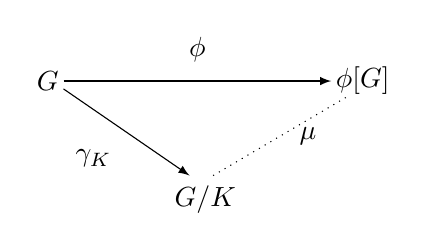
\begin{tikzpicture}
		\draw (0,1.5) node {$G$};
		\draw (2,0) node {$G/K$};
		\draw (4,1.5) node {$\phi[G]$};
		\draw[-latex] (0.2,1.4) -- node(e1)[sloped,label=below:$\gamma_K$]{} (1.8,0.3);
		\draw[-latex] (0.2,1.5) -- node(e2)[label=above:$\phi$]{} (3.6,1.5);
		\draw[dotted] (2.1,0.3) -- node(e2)[label=right:$\mu$]{} (3.8,1.3);
	\end{tikzpicture}
	\caption{First Isomorphism Theorem}
\end{figure}

\subsection{Second Isomorphism Theorem}
\begin{definition}

	Join $H \vee N$ is the smallest subgroup of $G$ containing $HN$ where $HN = \{ hn : h \in H, n \in N\}$.
\end{definition}

\begin{lemma}
	Let $N$ be a normal subgroup of $G$ and let $\gamma : G \to G/N$ be the canonical homomorphism.
	Then the map $\phi$ from the set of normal subgroups of $G$ containing $N$ to the set of normal subgroup of $G/N$ given by $\phi(L) = \gamma[L]$ is one-to-one and onto.
\end{lemma}
\begin{proof}
	Let $G$ be a group and $N$ be a normal subgroup of $G$.
	Given that $\gamma : G \to G/N$ the canonical homomorphism.
	That is, $\gamma(g) = gN$ for every $g \in G$.
	Let $L,M$ be normal subgroups of $G$ containing $N$.
	Since homomorphism preserves normality, $\gamma(L)$ is a normal subgroup of $\gamma[G]$.

	Suppose $\phi(L) = \phi(M)$.
	By definition of $\phi$,
	\begin{equation*}
		\gamma[L] = \phi(L) = \phi(M) = \gamma[M]
	\end{equation*}
	Since $N$ is normal, $\gamma^{-1}(\gamma(g)) = gN$ for every $g \in G$.
	And
	\begin{equation*}
		\gamma^{-1}(\gamma[L]) = \gamma^{-1} \left( \bigcup_{g \in L} \gamma(g) \right) = \bigcup_{g \in L} \gamma^{-1}(\gamma(g)) = \bigcup_{g \in L} gN = L
	\end{equation*}
	for every point $g \in L$, the left coset $gN$ is contained in $L$. ($\because N \subgroup L$)
	Therefore,
	\begin{equation*}
		\gamma^{-1} (\phi(L))  = \gamma^{-1} (\gamma[L]) = L 
	\end{equation*}
	\begin{equation*}
		\gamma^{-1} (\phi(M)) = \gamma^{-1} (\gamma[M]) = M
	\end{equation*}
	Thus, $L = M$.
	Therefore, $\phi$ is injective.

	Let $H$ be a normal subgroup of $G/N$.
	Then $\gamma^{-1}(H)$ is a normal subgroup of $G$.
	We have, $eN \in H$ and $\gamma^{-1}(eN) = eN = N$.
	Thus, $N \subset \gamma^{-1}(H)$.
	Thus, there exists $\gamma^{-1}(H)$, a normal subgroup of $G$ containing $N$ such that $\phi(\gamma^{-1}(H)) = H$.
	Therefore, $\phi$ is surjective.
\end{proof}

\begin{lemma}
	If $N$ is a normal subgroup of $G$, then $H \cap N = HN = NH$.
	Furthermore, if $H$ is also normal in $G$, then $HN$ is normal in $G$.
\end{lemma}
\begin{proof}
	Let $G$ be a group and $N$ be a normal subgroup of $G$.
	Also let $H$ be a subgroup of $G$.\\
	Claim : $HN$ is a subgroup of $G$, ie, $HN \subgroup G$

	
\end{proof}

\begin{theorem}[second isomorphism]
	Let $H$ be a subgroup of $G$ and let $N$ be a normal subgroup of $G$.
	Then $(HN)/N \isomorphism H/(H\cap N)$.
\end{theorem}
\begin{proof}
\end{proof}

\subsection{Third Isomorphism Theorem}
\begin{theorem}[third isomorphism]
	Let $H$ and $K$ be normal subgroup of $G$ with $K \le H$.
	Then $G/H \isomorphism (G/K)/(H/K)$.
\end{theorem}
\begin{proof}
\end{proof}

\begin{figure}[h]
	\centering
	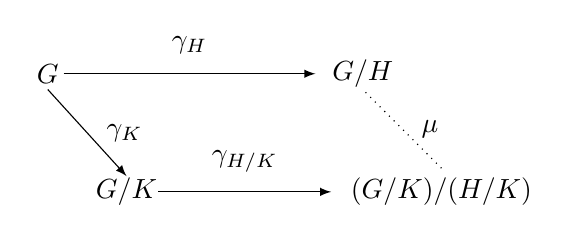
\begin{tikzpicture}
		\draw (0,1.5) node {$G$};
		\draw (1,0) node {$G/K$};
		\draw (5,0) node {$(G/K)/(H/K)$};
		\draw (4,1.5) node {$G/H$};
		\draw[-latex] (0,1.3) -- node(e1)[label=right:$\gamma_K$]{} (1,0.2);
		\draw[-latex] (0.2,1.5) -- node(e2)[label=above:$\gamma_H$]{} (3.4,1.5);
		\draw[-latex] (1.4,0) -- node(e3)[label=above:$\gamma_{H/K}$]{} (3.6,0);
		\draw[dotted] (5,0.3) -- node(e4)[label=right:$\mu$]{} (4,1.3);
	\end{tikzpicture}
	\caption{Third Isomorphism Theorem}
\end{figure}



\chapter{ME010102 Linear Algebra}
%Text Books : \cite{hoffman}
%Module 1:
%Vector spaces, subspaces, basis and dimension
%Co-ordinates, summary of row-equivalence, Computations concerning subspaces
%(Chapter 2- 2.1, 2.2, 2.3,2.4 2.5& 2.6 of the text) (20 hours)
%Module 2:
% Linear transformations, the algebra of linear transformations, isomorphism, representation of transformations by matrices, linear functional, double dual, transpose of a linear transformation.
%(Chapter 3 - 3.1, 3.2, 3.3, 3.4, 3.5, 3.6 & 3.7 of the text) (25 hours)
%Module 3:
%Determinants: Commutative Rings, Determinant functions, Permutation and uniqueness of determinants, Additional properties of determinants.
%(Chapter 5 - 5.1, 5.2, 5.3 & 5.4 of the text) (20 hours)
%Module 4:
%Introduction to elementary canonical forms, characteristic values, annihilatory Polynomials, invariant subspaces, Direct sum Decompositions
%(Chapter 6 - 6.1, 6.2, 6.3, 6.4,6.6of the text) (25 hours)

% \cite{hoffman} 2, 3, 5, 6
%Missing - 1, 4, 7, 8, 9, 10

%Module 1 - \cite{hoffman} 2
\section{Vector Spces}
%Module 2 - \cite{hoffman} 3
\section{Linear Transformations}
%Module 3 - \cite{hoffman} 5
\section{Determinants}
%Module 4 - \cite{hoffman} 6
\section{Elementary Canonical Forms}

\chapter{ME010103 Basic Topology}
%Text Books : \cite{joshi}
%Module I :
%Topological Spaces: Definition of a topological space – Examples of topological spaces-Bases and subbases – subspaces.
%(Chapter 4: Sections 1, 2, 3, and 4 of the text) (25 hours)
%Module II :
%Basic concepts: Closed sets and Closures – Neighbourhoods, Interior and
%Accumulation points – Continuity and Related Concepts – Making functions continuous , Quotient spaces
%( Chapter 5: Section 1;1. To 1.7 , Section 2; 2.1 to 2.10 and 2.13, Section3; 3.1 to 3.11, Theorem 3.2 condition 4 (25 hours)
%Module III :
%Spaces with special properties :- Smallness conditions on a space, Connectedness
%( Chapter 6 : Section 1; 1.1 to 1.16, Section 2; 2.1 to 2.15) (20 hours)
%Module IV :
%Spaces with special properties :- Local connectedness and Paths
%Separation axioms:- Hierarchy of separation axioms
%( Chapter 6 : Sections 3.1 to 3.8, Chapter 7 : Sections 1.1 to 1.17(20 hours)

%\chapter{Logical Warm-up*}
%\section{Statements and Their Truth values}
%\section{Negation, Conjunction, Disjunction and Truth Tables}
%\section{Deductions and Logical Precision}

%\chapter{Preliminaries}
%\section{Sets and Functions}
%\section{Sets with Additional Structures}
%\section{Preliminaries from Analysis}

%\chapter{Motivation for Topology}
%\section{What is Topology ?}
%\section{Geometry and Topology}
%\section{From Geometry to Metric Spaces}

%Introduction to topology game
%1. Open set characterisation
%Make four subsets of alphabets
%Letters of your name, and three of your friends names
%Intersection of any two sets - closed under finite intersections
%Union of any two sets - closed under arbitrary union
%2. Closed set characterisation
%Letters not in your name, and three of your friends names
%Union of any two sets - closed under finite unions
%Intersection of any two sets - closed under arbitrary intersections
%3. Neighbourhood Characterisation
%4. Interior Characterisation

%Need to find activities for the following :
%Continuous Function \& Quotient Space
%Compact, Lindeloff - Smallness of a Space
%Connected, Locally Connected, Path Connected
%Separation Axioms

%Need to give reading assignments:
%relevent skipped portions - what we might have missed !?
%other reference books - how they are presenting the same idea ?
%other books - get meaning out of it !

%\chapter{Topological Spaces}
%\section{Definition of a Topological Space}
%\section{Examples of Topological Spaces}
%\section{Bases and Sub-bases}
%\section{Subspaces}

%\chapter{Basic Concepts}
%\section{Closed Sets and Closure}
%\section{Neighbourhoods, Interior and Accumulation Points}
%\section{Continuity and Related Concepts}
%\section{Making Functions Continuous, Quotient Spaces}

%\chapter{Spaces with Special Properties}
%\section{Smallness Conditions on a Space}
%\section{Connectedness}
%\section{Local Connectedness and Paths}

%\chapter{Separation Axioms}
%\section{Hierarchy of Separation Axioms}

\chapter{ME010103 Real Analysis}
%Text Books: \cite{apostol}, \cite{rudin}
%Module 1: Functions of bounded variation and rectifiable curves
%Introduction, properties of monotonic functions, functions of bounded variation, total variation, additive property of total variation, total variation on $(a,x)$ as a functions of $x$, functions of bounded variation expressed as the difference of increasing functions, continuous functions of bounded variation, curves and paths, rectifiable path and arc length, additive and continuity properties of arc length, equivalence of paths, change of parameter.
%(Chapter 6, Section: 6.1 - 6.12. of \cite{apostol}) (20 hours.)
%Module 2: The Riemann-Stieltjes Integral
%Definition and existence of the integral, properties of the integral, integration and differentiation, integration of vector valued functions.
%(Chapter 6 - Section 6.1 to 6.25 of \cite{rudin}) (20 hours.)
%Module 3: Sequence and Series of Functions
%Discussion of main problem, Uniform convergence, Uniform convergence and Continuity, Uniform convergence and Integration, Uniform convergence and Differentiation.
%(Chapter 7 Section. 7.1 to 7.18 of \cite{rudin}) (25 hours.)
%Module 4: Weierstrass Approximation \& Some Special Functions
%Equicontinuous families of functions, the Stone - Weierstrass theorem, Power series, the exponential and logarithmic functions, the trigonometric functions, the algebraic completeness of complex field.
%(Chapter 7 – Sections 7.19 to 7.27, Chapter 8 - Section 8.1 to 8.8 of \cite{rudin}) (25 hours.)

%Module 1 - \cite{apostol} 6
%Module 2 - \cite{rudin} 6
%Module 3 - \cite{rudin} 7a
%Module 4 - \cite{rudin} 7b

%The commands to Riemann upper/lower integrals are defined by Leo Liu in tex-stack-exchange.
%Leo Liu - https://tex.stackexchange.com/a/44245 
\def\upint{\mathchoice%
    {\mkern13mu\overline{\vphantom{\intop}\mkern7mu}\mkern-20mu}%
    {\mkern7mu\overline{\vphantom{\intop}\mkern7mu}\mkern-14mu}%
    {\mkern7mu\overline{\vphantom{\intop}\mkern7mu}\mkern-14mu}%
    {\mkern7mu\overline{\vphantom{\intop}\mkern7mu}\mkern-14mu}%
  \int}
\def\lowint{\mkern3mu\underline{\vphantom{\intop}\mkern7mu}\mkern-10mu\int}

%Module 1
%\chapter{Functions of Bounded Variation \& Rectifiable Curves}
{\Large Module 1 : Bounded Variation \& Rectifiable Curves}
\section{Functions of Bounded Variation \& Rectifiable Curves}
%\subsection{Introduction}
\setcounter{subsection}{1}
\subsection{Properties of Monotone Functions}
\begin{theorem}
	Let $f$ be an increasing function defined on closed interval $[a,b]$.
	And let $x_0=a < x_1 < x_2 < \dots <x_{n-1} < x_n = b$.
	Then,
	\[ \sum_{k = 1}^{n-1} [f(x_k+)-f(x_k-)] \le f(b) - f(a) \]
\end{theorem}
\begin{proof}
	Let $f$ be an increasing function on $[a,b]$.
	Let $\{x_0=a,\ x_1, \dots,\ x_n=b\}$ be a partition of $[a,b]$.
	Let $y_k \in (x_{k-1},x_k),\ \forall k$.
	Then, $f(y_k) \le f(x_k+)$ and $f(x_k-) \le f(y_{k-1})$.
	Therefore,
	\[ \sum_{k=1}^{n-1} [f(x_k+) - f(x_k-)] \le \sum_{k=1}^{n-1} [f(y_k) - f(y_{k-1})] \le f(b) - f(a) \]
\end{proof}
\begin{commentary}
	In other words, for monotonic functions the sum of jumps is bounded.
\end{commentary}

\begin{theorem}
	Let $f$ be a monotonic function defined on closed interval $[a,b]$.
	Then the set of discontinuities of $f$ is countable.
\end{theorem}
\begin{proof}
	Without loss of generality, let $f$ be an increasing function on $[a,b]$.
	Let $S_m$ be the set of all points on $[a,b]$ at which the jump exceeds $\frac{1}{m}$.\\

	We know that, the sum of jumps of an increasing function is bounded above by $f(b)-f(a)$.	
	Thus, cardinality of $S_m$ given by,
	\[ |S_m| < m[f(b)-f(a)] \]
	is finite for any positive integer $m$.\\

	If $f$ is discontinuous at a pont $x \in [a,b]$, then there exists some integer $m'$ such that $0 < \frac{1}{m'} < x $ and $x \in S_{m'}$.
	\[ \text{Number of discontinuities } = \left| \bigcup_{m=1}^\infty S_m \right| \le \sum_{m=1}^\infty |S_m| \text{ is countable.}\]
	since countable sum of finite values is countable.
	Therefore, the number of discontinuities of $f$ is countable.
\end{proof}

\subsection{Function of Bounded Variation}
\begin{definition}[partition]
	Let $[a,b]$ be a compact interval.
	Let $x_0 = a$, $x_0 < x_1 < x_2 < \dots < x_n$ and $x_n = b$.
	Then $P = \{ x_0,x_1,\dots,x_n \}$ is a \textbf{partition} of $[a,b]$.
	And $(x_{k-1},x_k)$ is the \textbf{$k$th subinterval} of the partition.
\end{definition}

\begin{definition}[bounded variation]
	Let $f$ be a function defined on closed interval $[a,b]$.
	If there exists a positive real-number $M$ such that
	\[ \sum_{k=1}^n |\Delta f_k| = \sum_{k=1}^n |f(x_k) - f(x_{k-1})| \le M \]
	for any partition $P$ on $[a,b]$.
	Then $f$ is a function of \textbf{bounded variation}, where $(x_{k-1},x_k)$ is the $k$th subinterval of the partition.\\

\begin{commentary}
	In other words, a function is of bounded variation on $[a,b]$ if the sum of variations is bounded for any (finite) partition of $[a,b]$.
\end{commentary}
\end{definition}

\begin{theorem}
	Let $f$ be a monotonic function on $[a,b]$.
	Then $f$ is of bounded variation on $[a,b]$.
\end{theorem}
\begin{proof}
	Without loss of generality, let $f$ be an increasing function.
	Then for any partition $P = \{x_0,x_1,\dots,x_n\}$ of $[a,b]$, we have
	\[ \sum_{k=1}^n \left[ f(x_k)-f(x_{k-1}) \right] \le f(b)-f(a) = M \]
	Therefore, $f$ is of bounded variation on $[a,b]$.
\end{proof}

\begin{theorem}
	Let $f$ be a continuous function on $[a,b]$ and its derivative $f'$ exists and $f'$ is bounded in $(a,b)$.
	Then $f$ is of bounded variation.	
\end{theorem}
\begin{proof}
	Let $f$ be a continuous function with derivative $f'$ on $(a,b)$.
	Since $f$ is continuous and $f'$ exists, from intermediate value theorem we have
	\[ \Delta f_k = f(x_k) - f(x_{k-1}) = f'(t_k) [x_k-x_{k-1}] \text{ where } t_k \in (x_{k-1},x_k) \]
	Since $f'$ is bounded, $f'(t_k) \le M'$ for any $t_k \in (a,b)$.
	Thus,
	\[ \sum_{k=1}^n |\Delta f_k| = \sum_{k=1}^n |f'(t_k)| (x_k-x_{k-1}) \le M'\sum_{k=1}^n x_k-x_{k-1} = M'(b-a) = M \]
	Therefore, $f$ is of bounded variation.
\end{proof}

\begin{theorem}
	Let $f$ be a function on $[a,b]$.
	If $f$ is of bounded variation, then $f$ is bounded.
\end{theorem}
\begin{proof}
	Let $x \in (a,b)$.
	Consider the partition $P = \{ a,x,b \}$.
	Since $f$ is of bounded variation, there exists a positive real-number $M$ such that
	\[ \sum_{k=1}^2 |\Delta f_k| = |f(x)-f(a)| + |f(b)-f(x)| \le M \]
	Clearly, $|f(x)-f(a)| \le M$, since $|f(b)-f(x)| > 0$.
	We have,
	\[ |f(x)| = |f(x)-f(a)+f(a)| \le |f(x)-f(a)|+|f(a)| \le M+|f(a)| \]
	Suppose $x = a$, then $|f(x)| = |f(a)|$.\\
	Suppose $x = b$, then $|f(x)| = |f(b)| = M' + |f(a)|$ where $M' = |f(b)|-|f(a)|$.\\

	Therefore, the function $f$ is bounded on $[a,b]$.
\end{proof}

\subsection{Total Variation}
\begin{definition}[total variation]
	Let $f$ be a function of bounded variation on $[a,b]$.
	Let $\Sigma (P)$ be the sum of variations with respect to the partition $P$ of $[a,b]$.
	Then the \textbf{total variation} of the function $f$ on $[a,b]$ is given by,
	\[ V_f(a,b) = V_f = \sup \{ \Sigma (P) : P \in \mathscr{P}[a,b] \} \]
\end{definition}
\textbf{Note 1} : $V_f$ is finite, since $f$ is of boundned variation on $[a,b]$.\\

\textbf{Note 2} : $V_f \ge 0$, since $|\Delta f_k| \ge 0$ for any subinterval of $[a,b]$.\\


\textbf{Note 3} : $V_f = 0$ if only if $f$ is a constant function on $[a,b]$. (Why ?)

\begin{theorem}
	Let $f,g$ be functions of bounded variation on $[a,b]$.
	Then their sum $f+g$, difference $f-g$, and product $fg$ are of bounded variation.
	Also, 
	\[ V_{f \pm g} \le V_f + V_g \quad \text{ and } \quad V_{fg} \le AV_f + BV_g \]
	where $\displaystyle A = \sup \left\{ |g(x)| : x \in [a,b] \right\}$ and $\displaystyle B = \sup \left\{ |f(x)| : x \in [a,b] \right\}$.
\end{theorem}
\begin{proof}
	Let $f,g$ be functions of bounded variation on $[a,b]$.
	Then $f,g$ are bounded and $\sup |f(x)|$ and $\sup |g(x)|$ exists.\\

	\textbf{Step 1 : $V_{f \pm g} \le V_f + V_g$}\\
	We have,
	\[ |(f+g)(x_k) - (f+g)(x_{k-1})| \le | f(x_k) - f(x_{k-1})| + |g(x_k) - g(x_{k-1})| \]
	Then
	\begin{align*}
	V_{f+g}  
		& = \sup_{P \in \mathscr{P}} \sum_{k=1}^n |(f+g)(x_k) - (f+g)(x_{k-1})| \\
		& \le \sup_{P \in \mathscr{P}} \sum_{k=1}^n |f(x_k) - f(x_{k-1})| + \sup_{P \in \mathscr{P}} \sum_{k=1}^n |g(x_k)-g(x_{k-1})| \\
		& = V_f + V_g 
\end{align*}
	Similarly, we have $V_{f-g} \le V_f + V_g$ since
	\[ |(f-g)(x_k) - (f-g)(x_{k-1})| \le |f(x_k)-f(x_{k-1})| + |g(x_k)-g(x_{k-1})| \]

	\textbf{Step 2 : $V_{fg} \le AV_f + BV_g$}\\
	We have,
	\begin{align*}
	|fg(x_k)-fg(x_{k-1})| 
		& = |f(x_k)g(x_k) - f(x_{k-1}g(x_{k-1})| \\
		& = |f(x_k)g(x_k) - f(x_{k-1})g(x_k) + f(x_{k-1}g(x_k) - f(x_{k-1}g(x_{k-1}) | \\
		& \le |g(x_k)|\ |f(x_k)-f(x_{k-1})| + |f(x_{k-1}|\ |g(x_k) - g(x_{k-1})| \\
		& \le A |f(x_k)-f(x_{k-1})| + B |g(x_k)-g(x_{k-1})|
	\end{align*}
	where $A = \sup \{ |g(x)| : x \in [a,b] \}$ and $B = \sup \{ |f(x)| : x \in [a,b] \}$.\\

	Therefore,
	\begin{align*}
	V_{fg} 
		& \le A \sup_{P \in \mathscr{P}} \left\{ \sum_{k=1}^n |f(x_k)-f(x_{k-1}| \right\} + B \sup_{P \in \mathscr{P}} \left\{ \sum_{k=1}^n |g(x_k)-g(x_{k-1})| \right\} \\
		& = AV_f + BV_g 
	\end{align*}
\end{proof}

\begin{definition}[bounded away from zero]
	A function $f$ is bounded away from zero on $[a,b]$ if there exists a real-number $m$ such that $0 < m \le f(x)$, $\forall x \in [a,b]$.
\end{definition}

\begin{commentary}
	Let $f$ be a function of bounded variation.
	Then $\frac{1}{f}$ is of bounded variation if and only if $f$ is bounded away from zero.(Why ?)
\end{commentary}

\begin{theorem}
	Let $f$ be a function of bounded variation on $[a,b]$ and $f$ is bounded away from zero.
	Then, $g = \frac{1}{f}$ is a function of bounded variation on $[a,b]$ and $V_g \le \frac{V_f}{m^2}$ whenever $0 < m \le |f(x)|$.
\end{theorem}
\begin{proof}
	Suppose $f$ is of bounded variation on $[a,b]$ and $f$ is bounded away from zero.
	That is, there exists positive real-number $m$ such that $0 < m \le |f(x)|$, $\forall x \in [a,b]$.
	Then, $\frac{1}{|f(x)|} \le \frac{1}{m}$, $\forall x \in [a,b]$.\\

	Define $g = \frac{1}{f}$.
	Then, we have
	\[ |\Delta g_k| = \left| \frac{1}{f(x_k)} - \frac{1}{f(x_{k-1})} \right| = \frac{|f(x_k)-f(x_{k-1})|}{|f(x_k)|\ |f(x_{k-1}|} \le \frac{|f(x_k)-f(x_{k-1})|}{m^2} \]
	The total variation of $g$ on $[a,b]$ is given by,
	\begin{align*}
	V_g 
		& = \sup_{P \in \mathscr{P}} \left\{ \sum_{k=1}^n |g(x_k)-g(x_{k-1})| \right\} \\
		& \le \frac{1}{m^2} \sup_{P \in \mathscr{P}} \left\{ \sum_{k=1}^n |f(x_k)-f(x_{k-1})| \right\} \\
		& \le \frac{V_f}{m^2} \text{ where } 0 < m \le |f(x)|,\ \forall x \in [a,b]
	\end{align*}
\end{proof}
\begin{commentary}
	In other words, if $h,f$ are functions of bounded variation of $[a,b]$.
	And $f$ is bounded away from zero, then $g = \frac{1}{f}$ and $\frac{h}{f} = hg$ is a function of bounded variation and $V_{\frac{h}{f}} = V_{hg} \le AV_h + BV_f$.\\

	Now, we have analyzed sum, difference, product and quotient of functions of bounded variation.
	And we are not surprised about preservation of bounded variation under function composition. (Why ?)
\end{commentary}
\subsection{Additive Property of Total Variation}
\begin{theorem}[additive property]
	Let $f$ be a function of bounded variation on $[a,b]$.
	Let $c \in (a,b)$.
	Then $f$ is of bounded variation on both $[a,c]$ and $[c,b]$.
	And, $V_f(a,b) = V_f(a,c)+V_f(c,b)$.
\end{theorem}
\begin{proof}
	Let $f$ be a function of bounded variation on $[a,b]$.
	Let $P_1,P_2$ be partitions of $[a,c]$ and $[c,b]$ respectively.
	Then $P_0 = P_1 \cup P_2$ is a partition of $[a,b]$.
	Thus,
	\[ \sum (P_1) + \sum (P_2) = \sum (P_0) \le V_f(a,b) \]
	Taking supremums on the left side, we get
	\[ V_f(a,c) + V_f(c,b) \le V_f(a,b) \]	
	Clearly, $V_f(a,c) \le V_f(a,b)$ and $V_f(c,b) \le V_f(a,b)$.
	Therefore, function $f$ is of bounded variation on both $[a,c]$ and $[c,b]$.\\

	Let $P$ be a paritition of $[a,b]$.
	Then $P_0 = P\cup\{c\}$ is refinement of $P$.
	Now, we have two partitions $P_1, P_2$ of $[a,c]$ and $[c,b]$ such that $P_0 = P_1 \cup P_2$.
	Thus,
	\[ \sum (P) \le \sum (P_0) = \sum (P_1) + \sum (P_2) \le V_f(a,c) + V_f(c,b) \]
	Taking supremum on the left side, we get
	\[ V_f(a,b) \le V_f(a,c) + V_f(c,b) \]
	Therefore,
	\[ V_f(a,b) = V_f(a,c) + V_f(c,b),\quad \forall c \in (a,b) \]
\end{proof}

\subsection{Total Variation on $[a,x]$ as a function of $x$}
\begin{commentary}
	By additive property, we have existence of $V_f(a,x)$ for every $x \in (a,b]$.
	Assigning $V(x) = V_f(a,x)$, we have a well-defined function on $(a,b]$.
\end{commentary}

\begin{theorem}
	Let $f$ be a function of bounded variation on $[a,b]$.
	Define $V : [a,b] \to \mathbb{R}$ given by,
	\[ V(x) = \begin{cases} V_f(a,x) & x \in (a,b] \\ 0 & x = a \end{cases} \]
	Then,
	\begin{enumerate}
		\item $V$ is an increasing function on $[a,b]$.
		\item $V-f$ is an increasing function of $[a,b]$.
	\end{enumerate}
\end{theorem}
\begin{proof}
	Suppose $x = a$.
	Then $V(x) = 0$ and $V(y) = V_f(a,y) \ge 0 = V(x)$.\\
	Suppose $x \ne a$.
	Then, $a < x < y \le b$.
	By additive property of total variation, we have $V(y) = V_f(a,y) = V_f(a,x)+V_f(x,y) = V(x) + V_f(x,y)$.
	Since $V_f(x,y) \ge 0$, we have $V(x) \le V(y)$.
	Therefore, $V$ is an increasing function on $[a,b]$.\\

	Define $D : [a,b] \to \mathbb{R}$ given by $D(x)  = (V-f)(x) = V(x) - f(x)$.
	Suppose $a \le x < y \le b$.
	Then, $D(y)-D(x) = V(y)-f(y)-V(x)+f(x) = [V(y)-V(x)] - [f(y)-f(x)]$.
	We have, $V(y) = V_f(a,y) = V_f(a,x)+V_f(x,y)$.
	Thus, $V(y)-V(x) = V_f(x,y)$.
	Also we have, $f$ is of bounded variation on $[x,y]$.
	Consider the trivial partition $P = \{ x,y\}$ of $[x,y]$.
	Then, we have $f(y) - f(x) = \sum (P) \le V_f(x,y)$.
	Thus, $D(y)-D(x) = V_f(x,y) - [f(y)-f(x)] \ge 0$.
	Therefore, $D = V-f$ is an increasing function on $[a,b]$.
\end{proof}

\subsection{Function of bounded variation expressed as the difference of increasing functions}
\begin{theorem}
	Let $f$ be a function on $[a,b]$.
	Function $f$ is of bounded variation on $[a,b]$ if and only if $f$ can be expressed as difference of two increasing functions.
\end{theorem}
\begin{proof}
	Let $f$ be a function of bounded variation, then $f = V-D$ where total variation $V$ and $D = V-f$ are both increasing.\\

	Let $f$ be function on $[a,b]$.
	Let $f = V-D$ where $V,D$ are increasing functions. 
	Then $V,D$ are of bounded variation, since monotonic functions on $[a,b]$ are of bounded variation.
	Also, we have $V-D$ is of bounded variation, since for any two functions of bounded variation their difference is also of bounded variation.
\end{proof}

\subsection{Continuous functions of bounded variation}
\begin{theorem}
	Let $f$ be a function of bounded variation on $[a,b]$. %Why it has to be of bounded variation ? For the existence of $V$ ?
	Let $V$ be the total variation function of $f$ defined on $[a,b]$.
	$f$ is continuous at a point if and only if $V$ is continuous at that point.
\end{theorem}
\begin{proof}
	Let $f$ be a function of bounded variation on $[a,b]$.
	Let $V$ be the total variation of $f$.
	Let $x,y \in [a,b]$, such that $x<y$.
	We have $V$ is an increasing function on $[a,b]$.
	And $f$ is difference of two increasing functions on $[a,b]$.
	Thus, $f(x+),\ f(x-),\ V(x+),\ V(x-)$ exists for any $x \in (a,b)$.
	It remains to prove that $V,f$ are continuous at $x \in (a,b)$.\\

	\textbf{Part 1 : $V$ continuous $\implies$ $f$ continuous}\\
	Suppose $x \ne a$, then $a<x<y\le b$.
	Let $P$ be any partition on $[a,x]$.
	Then there exists a partition $P'$ on $[a,y]$ such that $P \subset P'$.
	Consider, $P' = P\cup\{y\}$.
	Then, $V(y) > V(x)$ and $V(y)-V(x) \ge |f(y)-f(x)|$.
	Thus,
	\[ 0 \le |f(y)-f(x)| \le V(y)-V(x) \]
	The inequality is true for any $y>x$.
	Therefore,
	\[ 0 \le |f(x+)-f(x)| \le V(x+)-V(x) \text{ as } y \to x+ \]
	Similarly, let $a<z<x$.
	Then,
	\[ 0 \le |f(x)-f(x-)| \le V(x)-V(x-) \text{ as } z \to x- \]
	Clearly, if $V$ is continuous at $x$ then $f$ is continuous $x$.\\

	\textbf{Part 2 : $f$ continuous $\implies$ $V$ continuous}\\
	Suppose $f$ is continuous at $c \in (a,b)$.
	Let $\varepsilon > 0$.
	We have,
	\[ V_f(c,b) = \sup_{P \in \mathscr{P}} \sum (P) \]
	Thus, there exists a partition $P_1 \in \mathscr{P}[c,b]$ such that $V_f(c,b) - \frac{\varepsilon}{2} < \sum (P_1)$.
	Since $f$ is continuous at $c$, there exists $x_1 \in (c,b)$ such that $|f(x_1)-f(c)| < \frac{\varepsilon}{2}$.
	Then,
	\[ V_f(c,b) - \frac{\varepsilon}{2} < \frac{\varepsilon}{2} + V_f(x_1,b) \]
	We have,
	\begin{align*}
	V(x_1)-V(c) 
		& = V_f(a,x_1) - V_f(a,c) = V_f(c,x_1) \\
		& = V_f(c,b) - V_f(x_1,b) < \varepsilon
	\end{align*}
	Clearly, $V(c+h) \to V(c)$ as $h \to 0$.
	That is, $V(c+) = V(c),\ \forall c \in [a,b)$.
	Similarly we have,
	\[ V_f(a,c) = \sup_{P \in \mathscr{P}} \sum (P) \]
	And there exists $P_2 \in \mathscr{P}[a,c]$ such that
	\[ V_f(a,c) - \frac{\varepsilon}{2} < \sum (P_2) \]
	And there exists $x_2 \in (a,c)$ such that $|f(c)-f(x_2)| < \frac{\varepsilon}{2}$, since $f$ is continuous at $c$.
	Therefore,
	\[ V(c)-V(x_2) = V_f(a,c) - V_f(a,x_2) = V(x_2,c) < \varepsilon \]
	Thus, $V(c-) = V(c),\ \forall c \in (a,b]$.
	Therefore, $V$ is continuous at $c$.
\end{proof}
\begin{theorem}
	Let $f$ be a continuous function on $[a,b]$.
	Function $f$ is of bounded variation on $[a,b]$ if and only if $f$ can be expressed as difference of two increasing continuous functions.
\end{theorem}
\begin{proof}
	Let $f$ be a continuous function on $[a,b]$.
	Then total variation $V$ is a continuous increasing function on $[a,b]$.
	Clearly, $D = V-f$ is also a continuous, increasing function on $[a,b]$.
	Therefore, $f = V - D$ where $V,D$ are continuous, increasing functions.\\

	Let $V,D$ be continuous, increasing functions on $[a,b]$.
	Then $f = V-D$ is also a continuous function on $[a,b]$.
	We have, $V,D$ are increasing functions, therefore both $V,D$ are of bounded variation and their difference $f$ is also of bounded variation.
\end{proof}

\begin{commentary}
	Suppose $f$ is of bounded variation on $[a,b]$.
	Let $id : [a,b] \to [a,b]$ where $id(x) = x$.
	Then $V+id$ is a strictly increasing function and $D = V+id-f$ is also strictly increasing.
	Thus, any function of bounded variation on $[a,b]$ can be characterised as difference of two strictly increasing continuous functions on $[a,b]$.
\end{commentary}
\subsection{Curves and Paths}
\begin{definition}[path]
	Let $f : [a,b] \to \mathbb{R}^n$ be a continuous, vector-valued function.
	Then $f$ is a path in $\mathbb{R}^n$.
	And $f$ is a motion if $[a,b]$ is a time interval.
\end{definition}
\subsection{Rectifiable paths and Arc length}
\begin{definition}[rectifiable path]
	Let $f : [a,b] \to \mathbb{R}^n$ be a path in $\mathbb{R}^n$.
	Let $P = \{ t_0,t_1,\dots,t_m \}$ be a partition of $[a,b]$.
	\[ \Lambda_f (P) = \sum_{k=1}^m \| f(t_k) - f(t_{k-1}) \| = \sum_{k=1}^m \| \Delta f_k \| \]
	If $\Lambda_f (P)$ is bounded for any partition $P \in \mathscr{P}[a,b]$, then path $f$ is \textbf{rectifiable}.
	If $\Lambda_f (P)$ is unbounded, then $f$ is \textbf{nonrectifiable}.\\
\end{definition}
\begin{definition}[arc length]
	Let $f : [a,b] \to \mathbb{R}^n$ be a rectifiable path.
	Then \textbf{arc length} of path $f$ is given by,
	\[ \Lambda_f(a,b) = \sup_{P \in \mathscr{P}} \Lambda_f (P) \]
\end{definition}

\begin{theorem}
	A path $f : [a,b] \to \mathbb{R}^n$ is rectifiable if and only if each component $f_k$ of $f$ is of bounded variation on $[a,b]$.
	Let $V_k(a,b)$ be the total variation of $f_k$ on $[a,b]$.
	Then,
	\[ V_k(a,b) \le \Lambda_f(a,b) \le V_1(a,b) + V_2(a,b) + \dots + V_n(a,b) \]
\end{theorem}
\begin{proof}
	Let $x_j \in \mathbb{R}^n$ for $j = 1,2,\dots,m$.
	Then,
	\[ |x_r| \le \sqrt{\sum_{j=1}^n |x_j|^2} \le \sum_{j=1}^n |x_j| \text{ since } \sum_{j=1}^n x_j^2 \le \left(\sum_{j=1}^n x_j\right)^2 \]
	Let $f : [a,b] \to \mathbb{R}^n$ be a path in $\mathbb{R}^n$.
	Then $f = (f_1,f_2,\dots,f_n)$ where $f_k$'s are components of the path $f$.
	Let $P = \{ t_0,t_1,\dots,t_m \}$ be a partition of $[a,b]$.
	Now $f_r(t_j)-f_r(t_{j-1}) \in \mathbb{R}^n$ for each subinterval of $[a,b]$ and each component of $f$.
	Thus for each subinterval $(t_j,t_{j-1})$ we have,
	\[ |f_r(t_j)-f_r(t_{j-1})| \le \| f(t_j)-f(t_{j-1}) \| \le \sum_{j=1}^n |f_k(t_j)-f_k(t_{j-1})| \] 
	Adding inequalities for every subinterval of the partition, we get
	\[ \sum_{k=1}^m |f_k(t_j)-f_k(t_{j-1})| \le \sum_{k=1}^m \| f(t_j)-f(t_{j-1}) \| \le \sum_{k=1}^m \sum_{j=1}^n |f_k(t_j)-f_k(t_{j-1})| \] 
	Rearranging summation, we get
	\[ \sum (P) \le \Lambda_f (P) \le \sum_{j=1}^n \left( \sum (P)_{f_j} \right) \] 
	Suppose $f$ is a rectifiable path.
	Then $f$ has finite arc length $\Lambda_f (a,b)$.
	Let $f_k$ be a component function of $f$.
	Let $P$ be a partition of $[a,b]$.
	Then,
	\[ \sum (P) \le \Lambda_f(P) \le \Lambda_f (a,b) \]
	Thus, $\sum (P)$ is bounded for any partition $P$.
	Therefore, total variation $V_k(a,b)$ exists for each component function $f_k$.
	And $V_k(a,b) \le \Lambda_f(a,b)$.\\

	Suppose $f_k$'s are of bounded variation.
	Then \[ \Lambda_f(P) \le \sum_{j=1}^n \sum (P) \le \sum_{j=1}^n V_j(a,b) \] is bounded for any partition $P$.
	Thus, $f$ is rectifiable.
	And, arc length $\displaystyle \Lambda_f(a,b) \le \sum_{k=1}^n V_k (a,b)$.
	Combining the inequalities, we get
	\[ V_k(a,b) \le \Lambda_f(a,b) \le \sum_{j=1}^n V_j (a,b) \]
\end{proof}
\subsection{Additive and Continuity Properties of Arc length}
\begin{theorem}[additive]
	Let $f : [a,b] \to \mathbb{R}^n$ be a rectifiable path.	
	Let $c \in (a,b)$.
	Then,
	\[ \Lambda_f(a,b) = \Lambda_f(a,c) + \Lambda_f(c,b) \]
\end{theorem}
\begin{proof}
	Let $P$ be a partition of $[a,b]$.
	Then $P' = P \cup \{c\}$ is a refinement of $P$ such that $P' = P_1 \cup P_2$ where $P_1,P_2$ are partition of $[a,c]$ and $[c,b]$ respectively.
	We have,
	\[ \Lambda_f(P) \le \Lambda_f(P') = \Lambda_f(P_1) + \Lambda_f(P_2) \]
	This inequality if true for any partition of $[a,b]$.
	Thus,
	\[ \Lambda_f(a,b) \le \Lambda_f(a,c) + \Lambda_f(c,b) \]
	Let $P_1,P_2$ be partition of $[a,c]$ and $[c,b]$ respectively.
	Then,
	\[ \Lambda_f(P_1) + \Lambda_f(P_2) \le \Lambda_f(P) \le \Lambda_f(a,b) \]
	This inequality if true for any paritions on $[a,c]$ and $[c,b]$.
	Thus,
	\[ \Lambda_f(a,c) + \Lambda_f(c,b) \le \Lambda_f(a,b) \]
\end{proof}
\begin{theorem}[continuity]
	Let $f : [a,b] \to \mathbb{R}^n$ be  rectifiable path.
	Let function $s : [a,b] \to \mathbb{R}$ defined by
	\[ s(x) = \begin{cases} 0 & x = a \\ \Lambda_f(a,x) & x \in (a,b] \end{cases} \]
	Then,
	\begin{enumerate}
		\item function $s$ is continuous and increasing on $[a,b]$.
		\item if there is no subinterval of $[a,b]$ in which $f$ is constant, then $s$ is strictly increasing.
	\end{enumerate}
\end{theorem}
\begin{proof}
	Let $a \le x < y \le b$.
	Then, $s(y)-s(x) = \Lambda_f(x,y) = \Lambda(a,y) - \Lambda(a,x) \ge 0$.
	Therefore, $s$ in increasing.\\
	
	Suppose $f$ is not constant in any subinterval $[x,y]$ of $[a,b]$.
	Suppose $s$ is not strictly increasing.
	Then, there exists $x,y \in (a,b)$ such that $x < y$ and $s(y)-s(x) = 0$.
	Thus,
	\[ \Lambda_f(a,y) - \Lambda(a,x) = \Lambda_f(x,y) = 0 \]
	Thus, $V_k(x,y) = 0,\ \forall k$ which is a contradition since $f$ is not constant in $[x,y]$.
	Therefore, $s$ is strictly increasing.
\end{proof}
\subsection{Equivalence of path, Change of parameter}
\begin{definition}[change of parameter]
	Let $f:[a,b] \to \mathbb{R}^n$ be a path.
	Let $g : [c,d] \to \mathbb{R}^n$ be another path.
	Then $f,g$ are \textbf{equivalent} if there exists a continuous, real-valued function, $u : [c,d] \to [a,b]$ such that $g = f \circ u$.
	That is, $g(t) = f(u(t)),\ \forall t \in [c,d]$.
	In other words, $f,g$ are different parametric representations of a common graph.\\

	Function $u$ defines a change of parameter.
	If $u$ is strictly increasing, then $f,g$ are in the same direction.
	And $u$ is an orientation preserving change of parameter.
	If $u$ is strictly decreasing, then $f,g$ are in opposite directions.
	And $u$ is an orientation reversing change of parameter.
\end{definition}

\begin{theorem}[change of parameter]
	Let $f:[a,b] \to \mathbb{R}^n$ and $g : [a,b] \to \mathbb{R}^n$ be two paths.
	Let $f,g$ be both injective functions.
	Then $f$ and $g$ are equivalent if they have the same graph.
\end{theorem}
\begin{proof}
	Let $f : [a,b] \to \mathbb{R}^n$ and $g : [c,d] \to \mathbb{R}^n$ be continuous, injective, vector-valued functions.
	Suppose $f,g$ are equivalent paths, then $f,g$ have the same graph.\\

	Suppose $f,g$ have the same graph.
	Since $f$ is injective and continuous on its domain $[a,b]$, function $f^{-1}$ exists and is continuous on its graph.
	\[ \text{Define } u:[c,d] \to [a,b],\ u(t) = f^{-1}(g(t)) \]
	Then $u$ is continuous and $g(t) = f(u(t))$.
	Suppose $u$ is not a strictly monotonic function. 
	Since $u$ is continuous, there exists $t_1,t_2 \in [c,d]$ such that $u(t_1) = u(t_2)$.
	Then $f(u(t_1)) = f(u(t_2)) \implies g(t_1) = g(t_2)$ which is a contradiction since $g$ is injective on $[c,d]$.
\end{proof}

%Module 2
%\chapter{The Riemann Stieltjes Integral} %Rudin chapter 6$
\pagebreak
{\Large Module 2 : Riemann-Stieltjes Integral}\\
\section{The Riemann-Stieltjes Integral}
\begin{definition}[unti step]
	The unit step function $I : \mathbb{R} \to \mathbb{R}$ is defined by
	\[ I(x) = \begin{cases} 0 & x \le 0 \\ 1 & x > 0 \end{cases} \] 
\end{definition}
\begin{definition}[Riemann Integral]
	Let $f$ be a bounded real function defined on $[a,b]$.
	Let $P = \{x_0,x_1,\dots,x_n\}$ be a partition of $[a,b]$.
	Let $M_k = \sup \{ f(x) : x \in [x_{k-1},x_k] \}$ and $m_k = \inf \{ f(x) : x \in [x_{k-1},x_k]$.\\

	Then Riemann upper sum of function $f$ with respect to parition $P$,
	\[ U(P,f) = \sum_P M_k \Delta x_k = \sum_{k=1}^n M_k (x_k-x_{k-1}) \]
	And Riemann lower sum of $f$ with respect to $P$,
	\[ L(P,f) = \sum_{k=1}^n m_k (x_k-x_{k-1}) \]
	Now, Riemann upper integral of $f$ over $[a,b]$,
	\[ \upint_a^b f\ dx = inf \{ U(P,f) : P \in \mathscr{P}[a,b] \} \]
	And, Riemann lower integral of $f$ over $[a,b]$,
	\[ \lowint_a^b f\ dx = sup \{ L(P,f) : P \in \mathscr{P}[a,b] \} \]
	A function $f$ is Riemann integrable over $[a,b]$ if Riemann lower and upper integrals of $f$ over $[a,b]$ are the same.
	Then Riemann integral of $f$ over $[a,b]$,
	\[ \int_a^b f\ dx = \upint_a^b f\ dx = \lowint_a^b f\ dx \]
\end{definition}
\begin{definition}[Riemann-Stieltjes Integral]
	Let $f$ be a bounded function on $[a,b]$.
	Let $\alpha$ be an increasing function on $[a,b]$.
	Let $P = \{ x_0,x_1,\dots,x_n\}$ be a partition of $[a,b]$.
	Then, the Riemann-Stieltjes upper sum of $f$ with respect to partition $P$ and increasing function $\alpha$,
	\[ U(P,f,\alpha) = \sum_{k=1}^n M_k \Delta \alpha_k \]
	where $M_k = \sup \{ f(x) : x \in [x_{k-1},x_k] \}$ and $\Delta \alpha_k = \alpha(x_k) - \alpha(x_{k-1})$.
	Similarly, Riemann-Stieltjes lower sum,
	\[ L(P,f,\alpha) = \sum_{k=1}^n m_k \Delta \alpha_k \]
	where $m_k = \inf \{ f(x) : x \in [x_{k-1},x_k] \}$.
	And function $f$ is Riemann-Stieltjes integrable if Riemann Stieltjes upper and lower integrals are the same.
	\[ \int_a^b f\ d\alpha = \upint_a^b f\ d\alpha = \lowint_a^b f\ d\alpha \]
	where $\displaystyle \upint_a^b f\ d\alpha = \upint_a^b f\ d\alpha(x) = \inf \left\{ U(P,f,\alpha) : P \in \mathscr{P}[a,b] \right\}$ and\\
	$\displaystyle \lowint_a^b f\ d\alpha = \sup \left\{ L(P,f,\alpha) : P \in \mathscr{P}[a,b] \right\}$.\\

	We write $f \in \mathscr{R}(\alpha)$ on $[a,b]$, which means that a bounded, real function $f$ is Riemann-Stieltjes integrable on $[a,b]$ with respect to the increasing function $\alpha$.
\end{definition}

\textbf{Note : } function $\alpha : [a,b] \to \mathbb{R}$ is monotonic (increasing), but not necessarily continuous.\\

\textbf{Remark : } With $\alpha = id$ identity function, Riemann-Stieltjes integral is Riemann integral itself.
	That is, Riemann integral is a special case of Riemann-Stieltjes integral.

\begin{theorem}
	Let $P^\ast$ be a refinement of a parition $P$ of $[a,b]$.
	Then, $L(P,f,\alpha) \le L(P^\ast,f,\alpha)$ and $U(P^\ast,f,\alpha) \le U(P,f,\alpha)$.
\end{theorem}
\begin{proof}
	Let $P^\ast = P \cup \{ x \}$ where $x$ belongs to the $i$th subinterval $(x_{j-1},x_j)$.
	Define $w_1 = \min \{ f(x) : x \in (x_{j-1},x) \}$ and $w_2 = \min \{ f(x) : x \in (x,x_j) \}$.
	Clearly, $w_1,w_2 \ge \min \{ f(x) : x \in (x_{j-1},x_j) \} = m_i$.
	\begin{align*}
	L(P,f,\alpha) - L(P^\ast,f,\alpha) 
		& = m_i \Delta \alpha_j - w_1 (\alpha(x)-\alpha(x_{j-1})) - w_2 (\alpha(x_j) - \alpha(x)) \\
		& = (m_i - w_1)(\alpha(x)-\alpha(x_{j-1})) + (m_i - w_2)(\alpha(x_j)-\alpha(x))\\
		& \ge 0
	\end{align*}
	By mathematical induction the inequality is true for any refinement $P^\ast$ of $P$.
	Therefore, $L(P,f,\alpha) \ge L(P^\ast,f,\alpha)$.\\

	Similarly, define $W_1 = \max \{f(x) : x \in (x_{j-1},x) \}$ and $W_2 = \max \{ f(x) : x \in (x,x_j) \}$
	where $W_1,W_2 \le \max \{ f(x) : x \in (x_{j-1},x_j) \} = M_i$.
	\begin{align*}
	U(P,f,\alpha) - U(P^\ast,f,\alpha) 
		& = M_i \Delta \alpha_j - W_1 (\alpha(x)-\alpha(x_{j-1})) - W_2 (\alpha(x_j) - \alpha(x)) \\
		& = (M_i - W_1)(\alpha(x)-\alpha(x_{j-1})) + (M_i - W_2)(\alpha(x_j)-\alpha(x))\\
		& \le 0
	\end{align*}
	Again, the result is true for any refinement $P$ and we have
	\[ U(P,f,\alpha) \le U(P^\ast,f,\alpha) \]
\end{proof}

\begin{theorem}
	Let $f$ be a bounded, real function on $[a,b]$ and $\alpha$ increasing function on $[a,b]$.
	Then,
	\[ \lowint_a^b f\ d\alpha \le \upint_a^b f\ d\alpha \]
\end{theorem}
\begin{proof}
	Let $P_1,P_2$ be any two partition of $[a,b]$.
	Let $P^\ast = P_1 \cup P_2$ be a refinement of both partitions.
	Then, we have $L(P^\ast,f,\alpha) \le U(P^\ast,f,\alpha)$.
	And,
	\[ \lowint_a^b f\ d\alpha \le L(P_1,f,\alpha) \text{ and } U(P_2,f,\alpha) \le \upint_a^b f\ d\alpha \]
	Therefore, \[ L(P_1,f,\alpha) \le L(P^\ast,f,\alpha) \le U(P^\ast,f,\alpha) \le U(P_2,f,\alpha) \]
	Clearly, the inequality holds independent of the choice of the partition.\\
	Taking supremum on right and infimum on left, we get
	\[ \sup_{P \in \mathscr{P}} L(P,f,\alpha) \le \inf_{ P \in \mathscr{P}} U(P,f,\alpha) \]
	Therefore,
	\[ \lowint_a^b f\ d\alpha \le \upint_a^b f\ d\alpha \]
\end{proof}

\begin{theorem}[criterion for integrability]
	Let $f$ be  a bounded, real function on $[a,b]$.
	Let $\alpha$ be an increasing function on $[a,b]$.
	Then, $f$ is Riemann-Stieltjes integrable on $[a,b]$ with repesct to $\alpha$ if and only if for every $\varepsilon > 0$ there exists a partition $P$ of $[a,b]$ such that $U(P,f,\alpha) - L(P,f,\alpha) < \varepsilon$.
\end{theorem}
\begin{commentary}
	In other words, $f \in \mathscr{R}(\alpha)$ on $[a,b]$ if and only if 
	\[ \forall \varepsilon > 0, \exists P \in \mathscr{P}[a,b] \text{ such that }U(P,f,\alpha) - L(P,f,\alpha) < \varepsilon \]
\end{commentary}
\begin{proof}
	Let $\varepsilon > 0$.
	Suppose there exists a partition $P$ of $[a,b]$ such that $U(P,f,\alpha) - L(P,f,\alpha) < \varepsilon$.
	We have,
	\[ L(P,f,\alpha) \le \lowint_a^b f\ d\alpha \le \upint_a^b f\ d\alpha \le U(P,f,\alpha) \]
	\[ \upint_a^b f\ d\alpha - \lowint_a^b f\ d\alpha \le U(P,f,\alpha)-L(P,f,\alpha) < \varepsilon \]
	Clearly, $\lowint_a^b f\ d\alpha = \upint_a^b f\ d\alpha$.
	Therefore, $f \in \mathscr{R}(\alpha)$.\\

	Suppose $f \in \mathscr{R}(\alpha)$ on $[a,b]$.
	Then by the definition of infimum there exists a partition $P_1$ of $[a,b]$ such that 
	\[ U(P_1,f,\alpha) - \upint_a^b f\ d\alpha < \frac{\varepsilon}{2} \]
	Similarly, there exists a partition $P_2$ of $[a,b]$ such that
	\[ \lowint_a^b f\ d\alpha - L(P_2,f,\alpha) < \frac{\varepsilon}{2} \]
	Consider $P^\ast = P_1 \cup P_2$.
	Clearly, $P^\ast$ is a refinement for both $P_1$ and $P_2$.
	Thus, \[ U(P^\ast,f,\alpha) - \upint_a^b f\ d\alpha < \frac{\varepsilon}{2} \]
	And,
	\[ \lowint_a^b f\ d\alpha - L(P^\ast,f,\alpha) < \frac{\varepsilon}{2} \]
	Thus, \[ U(P^\ast,f,\alpha) - \upint_a^b f\ d\alpha + \lowint_a^b f\ d\alpha - L(P^\ast,f,\alpha) < \varepsilon \]
	Given, $f \in \mathscr{R}(\alpha)$ on $[a,b]$.
	Therefore, $U(P^\ast,f,\alpha) - L(P^\ast,f,\alpha) < \varepsilon$.
\end{proof}

\begin{theorem}
	Suppose $\varepsilon > 0$ and $U(P,f,\alpha) - L(P,f,\alpha) < \varepsilon$ for some partition $P$ of $[a,b]$.
	\begin{enumerate}
		\item The inequaility is true for any refinement of $P$.
		\item Let $s_i,t_i \in [x_{i-1},x_i]$ for each subinterval of the partition $P$.
			\[ \sum_{i=1}^n \left| f_(s_i)-f(t_i) \right|\ \Delta\alpha_i < \varepsilon \]
		\item If $f \in \mathscr{R}(\alpha)$ and $t_i \in [x_{i-1},x_i]$ for each subinterval of the partition $P$, then
			\[ \left| \sum_{i=1}^n f(t_i) \Delta \alpha_i - \int_a^b f \ d\alpha \right| < \varepsilon \]
	\end{enumerate}
\end{theorem}
\begin{proof}
\begin{enumerate}
	\item Let $\varepsilon > 0$.
		Suppose $U(P,f,\alpha)-L(P,f,\alpha) < \varepsilon$.
		Let $P^\ast$ be a refinement of $P$.
		We have $U(P,f,\alpha) \ge U(P^\ast,f,\alpha)$ and $L(P,f,\alpha) \le L(P^\ast,f,\alpha)$.
		Thus,
		\[ U(P^\ast,f,\alpha)-L(P^\ast,f,\alpha) \le U(P,f,\alpha)-L(P,f,\alpha) < \varepsilon \]
	\item Let $s_i,t_i \in (x_{i-1},x_i)$.
		Clearly, for each subinterval $(x_{i-1},x_i)$, we have $m_i \le f(s_i) \le M_i$ and $m_i \le f(t_i) \le M_i$.
		Thus,
		\[ |f(t_i) - f(s_i)| \le  M_i - m_i \]
		\[ \sum_{i=1}^n |f(t_i) - f(s_i)| \Delta \alpha_i \le \sum_{i=1}^n (M_i - m_i) \Delta \alpha_i \le U(P,f,\alpha)-L(P,f,\alpha) \le \varepsilon \]
	\item Let $\varepsilon > 0$.
		Let $P$ be a partition of $[a,b]$ such that $U(P,f,\alpha) - L(P,f,\alpha) < \varepsilon$.
		We have,
		\[ L(P,f,\alpha) \le \lowint_a^b f\ d\alpha \le \upint_a^b f\ d\alpha \le U(P,f,\alpha) \]
		Suppose $f \in \mathscr{R}(\alpha)$ over $[a,b]$.
		Then, 
		\[ L(P,f,\alpha) \le \int_a^b f\ d\alpha \le U(P,f,\alpha) \] 

		Let $t_i \in (x_{i-1},x_i)$ for each subinterval of the partition $P$.
		Clearly, $m_i \le f(t_i) \le M_i$.
		Thus, we also have
		\[ L(P,f,\alpha) \le \sum_{i=1}^n f(t_i) \Delta \alpha_i \le U(P,f,\alpha) \]
		Therefore, 
		\[ \left| \sum_{i=1}^n f(t_i) \ \Delta \alpha_i - \int_a^b f\ d\alpha \right| \le U(P,f,\alpha) - L(P,f,\alpha) < \varepsilon \]
\end{enumerate}
\end{proof}
\begin{theorem}
	If $f$ is continuous on $[a,b]$, then $f \in \mathscr{R}(\alpha)$ on $[a,b]$.
\end{theorem}
\begin{proof}
	Let $f$ be a continuous function on $[a,b]$.
	Since continuous functions defined on compact subsets metric spaces are uniformly continuous, we have $f$ is uniformly continuous.\\

	Let $\varepsilon > 0$.
	Choose $\eta > 0$ such that $[\alpha(b)-\alpha(a)]\eta < \varepsilon$.
	Since $f$ is uniformly continuous, there exists $\delta > 0$ such that $|f(x)-f(t)| < \eta$ whenever $|x-t| < \delta$.	
	Consider the partition $P$ such that each subinterval is of length less than $\delta$.
	For any $s_i,t_i \in (x_{i-1},x_i)$, we have
	\begin{align*}
	\sum_{i=1}^n [f(t_i) - f(s_i)] \ [\alpha(x_i)-\alpha(x_{i-1})] 
		& \le \sum_{i=1}^n \eta [\alpha(x_i)-\alpha(x_{i-1})] \\
		& \le \eta \sum_{i=1}^n [\alpha(x_i)-\alpha(x_{i-1})] \\
		&	\le \eta[\alpha(b)-\alpha(a)] \\
		& < \varepsilon 
	\end{align*}
	Clearly, the result is true for minimum and maximum values of $f$ in each subinterval of $P$.
	Therefore, we have
	\[ U(P,f,\alpha) - L(P,f,\alpha) < \varepsilon \]
	Thus, $f \in \mathscr{R}(\alpha)$ over $[a,b]$.
\end{proof}

\begin{theorem}
	If $f$ is monotonic on $[a,b]$ and $\alpha$ is continuous on $[a,b]$, then $f \in \mathscr{R}(\alpha)$ on $[a,b]$.
\end{theorem}
\begin{proof}
	Let $f$ be increasing on $[a,b]$.
	Let $\alpha$ is continuous on $[a,b]$.
	Let $n$ be any integer.
	We can construct a partition $P$ of $[a,b]$ such that each the variation of $\alpha$ in each subinterval is fixed.
	That is, $\Delta \alpha_i = \frac{\alpha(b)-\alpha(a)}{n}$.
	Since $f$ is increasing, in each subinterval $[x_{i-1},x_i]$, we have $M_i = f(x_i)$ and $m_i = f(x_{i-1})$.
	Now we have,
	\begin{align*}
	U(P,f,\alpha) - L(P,f,\alpha) 
		& = \sum_{i=1}^n M_i \Delta \alpha_i - \sum_{i=1}^n m_i \Delta \alpha_i \\
		& = \sum_{i=1}^n (M_i-m_i) \Delta \alpha_i \\
		& = \frac{\alpha(b)-\alpha(a)}{n} \sum_{i=1}^n (f(x_i) - f(x_{i-1})) \\
		& = \frac{\alpha(b)-\alpha(a)}{n} (f(b)-f(a))
	\end{align*}
	Thus, given $\varepsilon > 0$, there exists an integer $n$ such that $ (\alpha(b)-\alpha(a))(f(b)-f(a)) < n\varepsilon $.
	And, we get a partition $P$ by fixing $\Delta \alpha_i = \frac{\alpha(b)-\alpha(a)}{n}$ such that $ U(P,f,\alpha)-L(P,f,\alpha) < \varepsilon $.\\

	In other words, $U(P,f,\alpha)-L(P,f,\alpha)$ depends on $n$ and can be reduced to a value less than $\varepsilon$ by increasing the value of $n$.
	Therefore, $f \in \mathscr{R}(\alpha)$ over $[a,b]$.
\end{proof}

\begin{theorem}
	If $f$ bounded on $[a,b]$, $f$ has only finitely many points of discontinuities on $[a,b]$ and $\alpha$ is continuous at every point at which $f$ is discontinuous.
	Then $f \in \mathscr{R}(\alpha)$.
\end{theorem}
\begin{proof}
	Suppose $f$ is bounded and has only finitely many discontinuities on $[a,b]$.
	Since $f$ is bounded, we have $-M < f(x) < M$ for some real number $M$.
	Also, suppose that $\alpha$ is continuous at those points where $f$ is discontinuous on $[a,b]$.\\

	Let $E$ be the set of all discontinuitites of $f$ on $[a,b]$.
	Clearly, $|E|$ is finite.\\

	Let $\varepsilon > 0$.
	Since, $\alpha$ is continuous at each point $e_j$ of $E$, \textcolor{blue}{there exists open intervals $(u_j,v_j)$ such that $\alpha$ is continuous on those intervals, $e_j$ belongs to the interior of these intervals and the sum of variation of $\alpha$ in those intervals is less than $\varepsilon$.}\\

	Removing these open intervals from $[a,b]$, we get a compact subset $K$ in which $f$ is continuous.
	Since $K$ is compact and $f$ is continuous on $K$, we have $f$ is uniformly continuous on $K$.\\

	Given $\varepsilon > 0$, there exists $\delta > 0$ such that $|f(x)-f(t)| < \varepsilon$ whenever $|x-t|<\delta$.
	Define a partition $P$ such that $u_j,\ v_j \in P$, $P$ doesn't have any point in the interior of any $(u_j,v_j)$.
	And if $x_{i-1} \ne u_j$, then $x_i$ is so choosen that $x_i-x_{i-1} < \delta$, dividing $K$ into subintervals of length less than $\delta$.
	Now, we have
	\begin{align*}
	U(P,f,\alpha) & - L(P,f,\alpha)
		 = \sum_{i=1}^n (M_i-m_i) \Delta \alpha_i  \\
		& \le \varepsilon \sum_{x_{i-1} \ne u_j} \Delta\alpha_i + 2M\sum_{x_{i-1} = u_j} \Delta\alpha_i \\
		& = \varepsilon \sum_{x_{i-1} \ne u_j} \left(\alpha(x_i)-\alpha(x_{i-1}) \right) + 2M\varepsilon \\
		& \le \varepsilon (\alpha(b)-\alpha(a)) + 2M\varepsilon
	\end{align*}
	Clearly, $U(P,f,\alpha)-L(P,f,\alpha)$ is a function of $\varepsilon$ which can reduced below any real number greater than zero by reducing the value of $\varepsilon$.
	Therefore, $f \in \mathscr{R}(\alpha)$ over $[a,b]$.
\end{proof}

\begin{theorem}
	Suppose $f \in \mathscr{R}(\alpha)$, $m \le f \le M$ on $[a,b]$, $\phi$ is continuous on $[m,M]$ and $h(x) = \phi(f(x))$.
	Then $h \in \mathscr{R}(\alpha)$ on $[a,b]$.
\end{theorem}
\begin{proof}
	Let $f$ be a function on $[a,b]$ such that $m \le f(x) \le M$ and $f \in \mathscr{R}(\alpha)$ over $[a,b]$.
	Let $\phi$ be  continuous function on $[m,M]$.
	Then $\phi$ is uniformly continuous on $[m,M]$, since $[m,M]$ is compact.
	Thus, given $\varepsilon > 0$ there exists $\delta > 0$ such that $|\phi(x)-\phi(t)| < \varepsilon$ whenever $|x-t|<\delta$.
	Without loss of generality, we may assume that $\delta < \varepsilon$.
	Otherwise choose a value less than $\varepsilon$ as $\delta$.\\

	Since $f \in \mathscr{R}(\alpha)$ over $[a,b]$, there exists a partition $P$ of $[a,b]$ such that
	\[ U(P,f,\alpha) - L(P,f,\alpha) < \delta^2 \]
	Consider the $i$th subinterval $[x_{i-1},x_i]$ of the partition $P$.
	Let $M_i$, $m_i$ be the maximum and minimum values of the function $f$ in $i$th subinterval of $P$.
	Now, we divided the collection of subintervals into two sets depending on the value of $M_i-m_i$ in comparison with $\delta$.
	Define $A$ as the set of all subintervals of $P$ such that $M_i-m_i < \delta$.
	And $B$ as the set of all subintervals of $P$ such that $M_i - m_i \ge \delta$.
	We know that,
	\[ \delta \sum_B \Delta \alpha_i \le \sum_B (M_i-m_i) \Delta \alpha_i < U(P,f,\alpha)-L(P,f,\alpha) < \delta^2 \]
	Thus, $\displaystyle \sum_B \Delta \alpha_i < \delta$.\\

	Define $M_i^\ast$, $m_i^\ast$ as the maximum and minimum of the function $\phi \circ f$ each subinterval $[x_{i-1},x_i]$ of the partition $P$.
	Now, we have
	\begin{align*}
	U(P,\phi \circ f,\alpha) - L(P,\phi \circ f, \alpha)
		& = \sum_{i=1}^n (M_i^\ast - m_i^\ast) \Delta \alpha_i \\
		& = \sum_A (M_i^\ast - m_i^\ast) \Delta \alpha_i + \sum_B (M_i^\ast - m_i^\ast) \Delta \alpha_i 
		\intertext{Since $\phi$ is uniformly continuous,}
		& \le \varepsilon \sum_A \Delta \alpha_i + \sum_B (M_i^\ast-m_i^\ast)\Delta \alpha_i 
	\intertext{Since, continuous functions defined on compact subset attains extrema. We have, $K = \sup \{ |\phi(x)| : x \in [m,M] \}$. And $M_i^\ast - m_i^\ast < 2K$.}
		& \le \varepsilon (\alpha(b)-\alpha(a)) + 2K \sum_B \Delta \alpha_i \\
		& \le \varepsilon (\alpha(b)-\alpha(a)) + 2K\delta \\
		& \le \varepsilon (\alpha(b) - \alpha(a)) + 2K\varepsilon
	\end{align*}
	Since $U(P,\phi \circ f,\alpha)-L(P,\phi \circ f, \alpha)$ is function of $\varepsilon$, it can be reduced to any sufficiently small real number of our choice.
	Therefore, $\phi \circ f \in \mathscr{R}(\alpha)$ over $[a,b]$.
\end{proof}

\subsection{Properties of the Riemann-Stieltjes Integral}
\begin{theorem}
	Let $f,f_1,f_2$ be bounded real functions on $[a,b]$.
	Let $\alpha,\alpha_1,\alpha_2$ be increasing functions on $[a,b]$.
	\begin{enumerate}
		\item If $f_1,f_2,f \in \mathscr{R}(\alpha)$ on $[a,b]$, then $f_1+f_2 \in \mathscr{R}(\alpha)$ on $[a,b]$.
			And,
			\[ \int_a^b \left( f_1 + f_2 \right)\ d\alpha = \int_a^b f_1\ d\alpha + \int_a^b f_2\ d\alpha \]
			If $c \in \mathbb{R}$, then $cf \in \mathscr{R}(\alpha)$ on $[a,b]$.
			And,
			\[ \int_a^b cf\ d\alpha = c\int_a^b f\ d\alpha \]
		\item If $f_1(x) \le f_2(x)$ on $[a,b]$, then
			\[ \int_a^b f_1\ d\alpha \le \int_a^b f_2\ d\alpha \]
		\item If $c \in (a,b)$, then $f \in \mathscr{R}(\alpha)$ on $[a,c]$ and $[c,b]$, then
			\[ \int_a^c f\ d\alpha + \int_c^b f\ d\alpha = \int_a^b f\ d\alpha \]
		\item If $|f(x)| \le M$ on $[a,b]$, then 
			\[ \left| \int_a^b f\ d\alpha \right| \le M[\alpha(b)-\alpha(a)] \]
		\item If $f \in \mathscr{R}(\alpha_1)$ and $f \in \mathscr{R}(\alpha_2)$ on $[a,b]$, then $f \in \mathscr{R}(\alpha_1+\alpha_2)$.
			And,
			\[ \int_a^b f\ d(\alpha_1+\alpha_2) = \int_a^b f\ d\alpha_1 + \int_a^b f\ d\alpha_2 \]
			If $f \in \mathscr{R}(\alpha)$ on $[a,b]$, and $c \in \mathbb{R}$, then $f \in \mathscr{R}(c\alpha)$ on $[a,b]$.
			And,
			\[ \int_a^b f\ d(c\alpha) = c\int_a^b f\ d\alpha \]
	\end{enumerate}
\end{theorem}
\begin{proof}
\begin{enumerate}
	\item Let $\varepsilon > 0$.
	Let $f_1,f_2 \in \mathscr{R}(\alpha)$ over $[a,b]$. \\
	Let $P_1$ be a partition of $[a,b]$ such that $U(P_1,f_1,\alpha) - L(P_1,f_1,\alpha) < \frac{\varepsilon}{2}$.\\
	Let $P_2$ be a partition of $[a,b]$ such that $U(P_2,f_2,\alpha) - L(P_2,f_2,\alpha) < \frac{\varepsilon}{2}$.\\
	Let $P = P_1 \cup P_2$ be the refinedment of both the partitions.
	Then the above inequalities are true of the partition $P$ as well.\\

	We have,
	\begin{align*}
	L(P,f_1,\alpha) + L(P,f_2,\alpha) 
		& \le L(P,f_1+f_2,\alpha) \\
		& \le U(P,f_1+f_2,\alpha) \\
		& \le U(P,f_1,\alpha) + U(P,f_2,\alpha) 
	\end{align*}
	Thus,
	\begin{align*}
	U(P,f_1+f_2,\alpha) & - L(P,f_1+f_2,\alpha)\\
		& \le U(P,f_1,\alpha) - L(P,f_1,\alpha) + U(P,f_2,\alpha) - L(P,f_2,\alpha) \\
		& \le \varepsilon
	\end{align*}
	Therefore, $f_1+f_2 \in \mathscr{R}(\alpha)$ over $[a,b]$.\\

	\hrule \vspace{1em}
	\item
	Let $c$ be any real number greater than zero.
	We have,
	\[ M_i' = \max \{ cf(x) : x \in [x_{i-1},x_i] \} = c \max \{ f(x) : x \in [x_{i-1},x_i] \} = cM_i \]
	Similarly, $m_i' = cm_i$.
	Thus,
	\[ \sum_{i=1}^n M_i'\Delta\alpha_i = c\sum_{i=1}^n M_i\Delta \alpha_i \text{ and } \sum_{i=1}^n m_i' \Delta\alpha_i = c\sum_{i=1}^n m_i \Delta\alpha_i \] 
	Therefore, given $\varepsilon > 0$ we have,
	\begin{align*}
		L(P,cf,\alpha) &= cL(P,f,\alpha) \\
		U(P,cf,\alpha) &= cU(P,f,\alpha)
	\end{align*}
	Since, $f \in \mathscr{R}(\alpha)$, there exists partition $P$ such that $U(P,f,\alpha)-L(P,f,\alpha) < \varepsilon$. Thus,
	\[ U(P,cf,\alpha)-L(P,cf,\alpha) = cU(P,f,\alpha)-cL(P,f,\alpha) < c\varepsilon \]
	Therefore, $cf \in \mathscr{R}(\alpha)$ over $[a,b]$.
	\begin{align*}
	\int_a^b cf\ d\alpha 
		& \le U(P,cf,\alpha) \\
		& \le cU(P,f,\alpha) \\
		& \le c \int_a^b f\ d\alpha + c\varepsilon\\
		& \le c\int_a^b f\ d\alpha
	\intertext{Similarly, considering $-f$ and $-cf$ we get}
	\int_a^b cf\ d\alpha 
		& \ge c\int_a^b f\ d\alpha
	\end{align*}
	Therefore, without loss of generality for any real number $c$, 
		\[ \int_a^b cf\ d\alpha = c\int_a^b f\ d\alpha \]

	\hrule \vspace{1em}
	\item 
	Let $\varepsilon > 0$.
	Suppose $f_1,f_2 \in \mathscr{R}(\alpha)$ and $f_1 \le f_2$.
	Let $P_1,P_2$ be the partitions such that $U(P_1,f_1,\alpha) - L(P_1,f_1,\alpha) < \varepsilon$ and $U(P_2,f_2,\alpha) - L(P_2,f_2,\alpha) < \varepsilon$.
	Consider the common refinement $P = P_1 \cup P_2$.
	Then, for each subinterval of the partition $P$, we have
	\[ \min_{x \in [x_{i-1},x_i]} f_1(x) \le \min_{x \in [x_{i-1},x_i]} f_2(x) \text{ and } \max_{x \in [x_{i-1},x_i]} f_1(x) \le \max_{x \in [x_{i-1},x_i]} f_2(x) \]
	Thus, $L(P,f_1,\alpha) \le L(P,f_2,\alpha)$ and $U(P,f_1,\alpha) \le U(P,f_2,\alpha)$.
	\begin{align*}
	\int_a^b f_1\ d\alpha 
		& \le U(P,f_1,\alpha) \\
		& \le U(P,f_2,\alpha) \\
		& \le \int_a^b f_2\ d\alpha + \varepsilon
	\end{align*}
	Therefore,
	\[ \int_a^b f_1\ d\alpha \le \int_a^b f_2\ d\alpha \]

	\hrule \vspace{1em}
	\item 
	Let $f \in \mathscr{R}(\alpha)$ on $[a,b]$.
	Let $\varepsilon > 0$.
	Then, there exists a parition $P$ of $[a,b]$ such that $U(P,f,\alpha) - L(P,f,\alpha) < \varepsilon$.
	Let $c \in (a,b)$.
	Then $P^\ast = P \cup \{c\} = P_1 \cup P_2$ is refinement of $P$ such that $P_1,P_2$ are partition of $[a,c]$ and $[c,b]$ respectively.
	Clearly, $U(P_1,f,\alpha) - L(P_1,f,\alpha) < \varepsilon$ and $U(P_2,f,\alpha) - L(P_2,f,\alpha) < \varepsilon$.
	Therefore, $f \in \mathscr{R}(\alpha)$ on both $[a,c]$ and $[c,b]$.\\

	For any two partitions $P_1,P_2$ of $[a,c]$ and $[c,b]$, there exists partition $P^\ast = P_1 \cup P_2$ of $[a,b]$.
	Thus,
	\begin{align*}
	\int_a^b f\ d\alpha 
		& \le U(P^\ast,f,\alpha) \\
		& \le U(P_1,f,\alpha) + U(P_2,f,\alpha) \\
		& \le \int_a^c f\ d\alpha + \int_c^b f\ d\alpha + 2\varepsilon
	\end{align*}
	Since $\varepsilon$ is arbitrary, we have
	\[ \int_a^b f\ d\alpha \le \int_a^c f\ d\alpha + \int_c^b f\ d\alpha \]
	And considering $-f$ instead of $f$, we get
	\[ \int_a^b -f\ d\alpha \le \int_a^c -f\ d\alpha + \int_c^b -f\ d\alpha \]
	Thus,
	\[ \int_a^b f\ d\alpha \ge \int_a^c f\ d\alpha + \int_c^b f\ d\alpha \]
	Therefore,
	\[ \int_a^b f\ d\alpha = \int_a^c f\ d\alpha + \int_c^b f\ d\alpha \]

	\hrule \vspace{1em}
	\item
	Let function $f \in \mathscr{R}(\alpha)$ on $[a,b]$ and $|f| \le M$.
	Let $P$ be any partition of $[a,b]$.
	We have, 
	\[ L(P,f,\alpha) \le \int_a^b f\ d\alpha \le U(P,f,\alpha)\]
	And,
	\[ L(P,f,\alpha) = \sum_{i=1}^n m_i \Delta \alpha_i \ge -M\Delta \alpha_i = -M \sum_{i=1}^n \Delta \alpha_i = -M[\alpha(b)-\alpha(a)] \]
	Similarly,
	\[ U(P,f,\alpha) = \sum_{i=1}^n M_i \Delta \alpha_i \le M\Delta \alpha_i = M \sum_{i=1}^n \Delta \alpha_i = M[\alpha(b)-\alpha(a)] \]
	Therefore,
	\[ \left| \int_a^b f\ d\alpha \right| \le M[\alpha(b)-\alpha(a)] \]
		
	\hrule \vspace{1em}
	\item
	Let $\alpha_1,\alpha_2$ be monotonic functions on $[a,b]$.
	Then $|\alpha_1 + \alpha_2 | \le |\alpha_1| + |\alpha_2|$.
	Let $f \in \mathscr{R}(\alpha_1)$ on $[a,b]$ and $f \in \mathscr{R}(\alpha_2)$ on $[a,b]$.
	Let $\varepsilon > 0$.
	Then there exists partitions $P_1,P_2$ of $[a,b]$ such that
	\[ U(P_1,f,\alpha_1) - L(P_1,f,\alpha_1) < \varepsilon \]
	\[ U(P_2,f,\alpha_2) - L(P_2,f,\alpha_2) < \varepsilon \]
	Consider the common refinement $P = P_1 \cup P_2$.
	Then, the inequalities are true for $P$ as well.
	And for each subinterval $[x_{i-1},x_i]$ of $P$, we have $\Delta(\alpha_1+\alpha_2)_i \le \Delta (\alpha_1)_i + \Delta (\alpha_2)_i$.
	Thus,
	\begin{align*}
	U(P,f,\alpha_1+\alpha_2) - L(P,f,\alpha_1+\alpha_2)
		& = \sum_{i=1}^n (M_i-m_i) \Delta (\alpha_1+\alpha_2)_i \\
		& \le \sum_{i=1}^n (M_i - m_i) \Delta \alpha_{1,i} + \sum_{i=1}^n (M_i-m_i) \Delta \alpha_{2,i} \\
		& \le 2\varepsilon
	\end{align*}
	Therefore, $f \in \mathscr{R}(\alpha_1+\alpha_2)$ on $[a,b]$.
	\begin{align*}
	\int_a^b f\ d(\alpha_1+\alpha_2) 
		& \le U(P,f,\alpha_1+\alpha_2) \\
		& \le U(P,f,\alpha_1) + U(P,f,\alpha_2) \\
		& \le \int_a^b f\ d\alpha_1 + \int_a^b f\ d\alpha_2 + 2\varepsilon
	\end{align*}
	Thus,
	\[ \int_a^b f\ d(\alpha_1+\alpha_2) \le \int_a^b f\ d\alpha_1 + \int_a^b f\ d\alpha_2 \]
	Considering $-f$ instead of $f$,we get
	\[ \int_a^b f\ d(\alpha_1+\alpha_2) \ge \int_a^b f\ d\alpha_1 + \int_a^b f\ d\alpha_2 \]
	Therefore,
	\[ \int_a^b f\ d(\alpha_1+\alpha_2) = \int_a^b f\ d\alpha_1 + \int_a^b f\ d\alpha_2 \]

	\hrule \vspace{1em}

	Let $c>0$ and $f \in \mathscr{R}(\alpha)$ on $[a,b]$.
	Let $\varepsilon > 0$.
	Then there exists a partition $P$ of $[a,b]$ such that $U(P,f,\alpha) - L(P,f,\alpha) < \varepsilon$.
	Clearly, $U(P,f,c\alpha) - L(P,f,c\alpha) < c\epsilon$.
	Therefore, $f \in \mathscr{R}(c\alpha)$ on $[a,b]$.
	\begin{align*}
	\int f d(c\alpha) 
		& \le U(P,f,c\alpha) \\
		& \le cU(P,f,\alpha) \\
		& \le c\int f d\alpha + c\varepsilon
	\end{align*}
	Thus,
	\[ \int f d(c\alpha) \le c \int f d\alpha \]
	Taking $-f$ instead of $f$, we get
	\[ \int f d(c\alpha) \ge c \int f d\alpha \]
	Therefore,
	\[ \int f d(c\alpha) = c \int f d\alpha \]
\end{enumerate}
\end{proof}

\begin{theorem}
If $f,g \in \mathscr{R}(\alpha)$ on $[a,b]$, then
\begin{enumerate}
	\item $fg \in \mathscr{R}(\alpha)$ on $[a,b]$
	\item $|f| \in \mathscr{R}(\alpha)$ on $[a,b]$.
	And,
	\[ \left| \int_a^b f\ d\alpha \right| \le \int_a^b |f|\ d\alpha \]
\end{enumerate}
\end{theorem}
\begin{proof}
\begin{enumerate}
	\item
	Let $f,g \in \mathscr{R}(\alpha)$ on $[a,b]$.
	By linearity of the integral we have $f+g \in \mathscr{R}(\alpha)$ on $[a,b]$.
	Let $\phi(t) = t^2$.
	Then $\phi$ is continuous.
	Thus, $\phi \circ f$ is continuous on $[a,b]$.
	Therefore, $\phi \circ f \in \mathscr{R}(\alpha)$ on $[a,b]$.
	{\color{blue}Also we have, $\phi \circ (f+g) = (f+g)^2$ and $\phi \circ (f-g) = (f-g)^2$.
	Thus, $(f+g)^2,(f-g)^2 \in \mathscr{R}(\alpha)$ on $[a,b]$.
	Now, $4fg = (f+g)^2 - (f-g)^2$.}
	Therefore, $4fg \in \mathscr{R}(\alpha)$ on $[a,b]$, from linearity of the integral.
	Take $c = \frac{1}{4}$, we get $fg \in \mathscr{R}(\alpha)$ on $[a,b]$ from linearlity of the integral.\\

	\hrule \vspace{1em}
	\item
	Let $f \in \mathscr{R}(\alpha)$ on $[a,b]$.
	Let $\phi(t) = |t|$.
	Then $\phi$ is continuous.
	Therefore, $\phi \circ f = |f| \in \mathscr{R}(\alpha)$ on $[a,b]$.\\

	{\color{blue}Let $c = \pm 1$ such that
	\[ c\int f d\alpha \ge 0 \]
	Then, 
	\[ \left|\int f d\alpha \right| = c\int f d\alpha = \int cf d\alpha \le \int |f| d\alpha \]
	since $cf \le |f|$. }
\end{enumerate}
\end{proof}

\begin{definition}[step]
	The unit step function, $I : \mathbb{R} \to [0,1]$ is defined by
		\[ I(x) = \begin{cases} 0 & x \le 0 \\ 1 & x > 0 \end{cases} \]
\end{definition}

\begin{theorem}
	Let $f$ be bounded on $[a,b]$ and continuous at $s \in (a,b)$.
	Let $\alpha = I(t-s)$.
	Then,
		\[ \int_a^b f d\alpha = f(s) \]
\end{theorem}
\begin{proof}
	Let $P = \{ a,s,x_2,b \}$ be a partition of $[a,b]$.
	Since $f$ is bounded, 
		\[ U(P,f,\alpha) = M_1 \Delta\alpha_1 + M_2 \Delta \alpha_2+ M_3 \Delta\alpha_3 = M_2 \]
	since $\Delta\alpha_1 = 0$, we have $\Delta\alpha_2 = \alpha(x_2) - \alpha(s) = I(x_2-s) - I(0) = 1-0$ and $\Delta \alpha_3 = 0$.
	Similarly, $L(P,f,\alpha) = m_1\Delta\alpha_1 + m_2\Delta\alpha_2 + m_3\Delta\alpha_3 = m_2$.
	We have,
		\[ m_2 = L(P,f,\alpha) \le \lowint_a^b f d\alpha \le \upint_a^b f d\alpha \le U(P,f,\alpha) = M_2 \]
	We know that, $M_2$ is the maximum value of $f$ in the subinteval $[s,x_2]$.
	The lower sum and upper sum remains the same as we reduce the length of the second subinterval.
	We also know that, $f$ is continuous at $s$.
	As $x_2 \to s$, the maximum value of $f$ tends to the value of $f$ at $s$, say $f(s)$.
	Similarly,  $m_2 \to f(s)$ as $x_2 \to s$.
	Thus,
		\[ f(s) \le \lowint_a^b f d\alpha \le \upint_a^b f d\alpha \le f(s) \]
	Therefore, $f \in \mathscr{R}(\alpha)$ on $[a,b]$ and
		\[ \int_a^b f d\alpha = f(s) \]
\end{proof}

\begin{theorem}
	Suppose $\displaystyle \sum_{i=1}^\infty c_n$ converges and $c_n \ge 0$.
	Let $f$ be continuous on $[a,b]$.
	Let sequence $\sequence{s_n}$ be a strictly increasing sequence in $(a,b)$.
	Let $\displaystyle \alpha = \sum_{i=1}^\infty c_n I(t-s_n)$.
	Then,
	\[ \int_a^b f\ d\alpha = \sum_{i=1}^\infty c_n f(s_n) \]
\end{theorem}
\begin{proof}
	Let $\sum_{n=1}^\infty c_n$ be a convergent series.
	Given $\varepsilon > 0$, there exists a natural number $N$ such that 
	\[ \sum_{n=N+1}^\infty c_n < \varepsilon \]
	Let $s_1,s_2,s_3,\dots$ be distinct points in $(a,b)$.
	Without loss of generality, sequence $\sequence{s_n}$ is a striclty increasing sequence in $[a,b]$.
	Let $\alpha = \sum_{n = 1}^\infty c_n I(t-s_n)$.
	Then, $\alpha(a) = 0$ and $\alpha(b) = \sum_{n=1}^\infty c_n$.
	\[ 0 \le \alpha(x) \le \sum_{n=1}^\infty c_n, \quad \forall x \in [a,b] \]
	By comparison test, $\alpha$ is convergent in $[a,b]$.
	We have,
	\[ \int_a^b f(t)\ d(c_1 I(t-s_1)) = c_1 \int_a^b f(t)\ d(I(t-s_1)) =  c_1 f(s_1) \]
	Let $\alpha = \alpha_1 + \alpha_2$ where $\displaystyle \alpha_1 = \sum_{n=1}^N c_n I(t-s_n)$ and $\displaystyle\alpha_2 = \sum_{n=N+1}^\infty c_n I(t-s_n)$.
	And from mathematical induction, we have
	\begin{align*}
	\int_a^b f(t) d(\alpha_1) 
		& = \int_a^b f(t)\ d\left( \sum_{n=1}^N c_n I(t-s_n) \right)\\
		& = \sum_{n=1}^N \int_a^b f(t)\ d(c_nI(t-s_n)) \\
		& = \sum_{n=1}^N c_n \int_a^b f dI(t-s_n) \\
		& = \sum_{n=1}^N c_n f(s_n) 
	\end{align*}
	We have,
	\[ \left| \int_a^b f(t) d\alpha_2 \right| \le M (\alpha_2(b) - \alpha_2(a)) = M \sum_{n=N+1}^\infty < M\varepsilon \]
	where $M = \sup |f(x)|$.
	Thus,
	\begin{align*}
	\left| \int_a^b fd\alpha_2 \right| 
		& = \left| \int_a^b f d(\alpha_1+\alpha_2) - \int_a^b fd\alpha_1 \right| \\
		& = \left| \int_a^b fd\alpha - \sum_{n=1}^N c_n f(s_n) \right| \\
		& < M\varepsilon 
	\end{align*}
	The inequality is true as $N \to \infty$. 
	In other words, the sequence of partial sums converges to the value of integral of $f$.
	Therefore,
	\[ \sum_{n=1}^\infty c_n f(s_n) = \int_a^b f d\alpha \]
\end{proof}

\begin{theorem}
	Let $\alpha$ be increasing function on $[a,b]$ and $\alpha' \in \mathscr{R}$.
	Let $f$ be bounded real-valued function on $[a,b]$.
	Then $f \in \mathscr{R}(\alpha)$ if and only if $f\alpha' \in \mathscr{R}$.
	And
	\[ \int_a^b f d\alpha = \int_a^b f(x)\alpha'(x) dx \]
\end{theorem}
\begin{proof}
	Since $\alpha' \in \mathscr{R}$ on $[a,b]$, for any $\varepsilon > 0$, there exists a partition $P$ of $[a,b]$ such that $U(P,\alpha')-L(P,\alpha') < \varepsilon$.
	We have, $\alpha$ is continuous on $[a,b]$, as it is differentiable on $[a,b]$.
	Then by intermediate value theorem, we have
	\[ \Delta \alpha_i = \alpha(x_i) - \alpha(x_{i-1}) = \alpha'(t_i) (x_i-x_{i-1}) \]
	where $t_i \in [x_{i-1},x_i]$.
	Let $s_i \in [x_{i-1},x_i]$.
	Then,
	\[ \sum_{i=1}^n |\alpha'(s_i) - \alpha'(t_i)|\Delta x_i \le U(P,\alpha') - L(P,\alpha') < \varepsilon \]
	Let $M = \sup |f|$.
	\textcolor{blue}{Let $u_i \in [x_{i-1},x_i]$.}
	\footnote{In my opinion, using $u_i$ instead of $s_i$ in the first sum makes it simpler.}
	Consider,
	\begin{align*}
	\left| \sum_{i=1}^n f(u_i) \Delta \alpha_i - \sum_{i=1}^n f(s_i) \alpha'(s_i) \Delta x_i \right| 
		& \le M \left| \sum_{i=1}^n \Delta \alpha_i - \alpha'(s_i) \Delta x_i \right| \\
		& \le M \left| \sum_{i=1}^n \alpha'(t_i) \Delta x_i - \alpha'(s_i) \Delta x_i \right| \\
		& \le M  \sum_{i=1}^n |\alpha'(t_i) - \alpha'(s_i)| \Delta x_i \\
		& < M \varepsilon 
	\end{align*}
	Clearly, the inequality is true independent of the choice of $u_i,s_i \in [x_{i-1},x_i]$.
	Thus, selecting $u_i$ such that $f(u_i) = M_i$, we get
	\[ \left| U(P,f,\alpha) - \sum_{i=1}^n \alpha'(s_i)\Delta x_i \right| < M\varepsilon \]
	Therefore,
	\[ \sum_{i=1}^n f(s_i) \alpha'(s_i) \Delta x_i < U(P,f,\alpha) + M\varepsilon \]
	Selecting $s_i$ such that $f\alpha'$ attains maximum at $s_i$, we get
	\[ U(P,f\alpha') < U(P,f,\alpha) + M\varepsilon \]
	Now, first we select $s_i$ such that $f\alpha(s_i)$ is maximum in $i$th subinterval of $P$.
	Then,
	\[ \left| \sum_{i=1}^n f(u_i) \Delta \alpha_i - U(P,f\alpha') \right| < M\varepsilon \]
	Therefore,
	\[ U(P,f\alpha') < \sum_{i=1}^n f(u_i) \Delta \alpha_i + M\varepsilon \]
	And, now selecting $u_i$ such that $f(u_i) = M_i$.
	\[ U(P,f\alpha') < U(P,f,\alpha) + M\varepsilon \]
	Therefore, we have $U(P,f\alpha') = U(P,f,\alpha)$.
	Clearly, it is true for any refinement of $P$.
	Therefore,
	\[ \upint_a^b f\alpha' dx = \upint_a^b f d\alpha \]
	Similary, by selecting $u_i$ and $s_i$ such that $f(u_i)$, $f\alpha'(s_i)$ is minimum in each subinterval of $P$, we get
	\[ \lowint_a^b f\alpha' dx = \lowint_a^b f d\alpha \]
	Cleary, $f \in \mathscr{R}(\alpha) \iff f\alpha' \in \mathscr{R}$. And,
	\[ \int_a^b f\alpha' dx = \int_a^b f d\alpha \]
\end{proof}

\begin{theorem}[change of variable]
	Let $\varphi : [A,B] \to [a,b]$ be a strictly increasing, continuous function onto $[a,b]$.
	Let $\alpha : [a,b] \to \mathbb{R}$ be an increasing function and $f \in \mathscr{R}(\alpha)$ on $[a,b]$.
	Define $\beta = \alpha \circ \varphi$ and $g = f \circ \varphi$.
	Then $g \in \mathscr{R}(\beta)$ on $[A,B]$ and 
	\[ \int_A^B g d\beta = \int_a^b f d\alpha \]
\end{theorem}
\begin{proof}
	Let $P = \{x_0,x_1,\dots,x_n\}$ be any partition of $[a,b]$.
	Then there exists a partition $Q = \{ y_0,y_1,\dots,y_n\}$ of $[A,B]$ such that $x_j = \varphi(y_j)$ since $\varphi$ is a continuous, bijection.
	\dag\footnote{Strictly increasing functions are always injective.}
	Similarly, for any partition $Q = \{ y_0,y_1,\dots,y_n\}$ of $[A,B]$, there exists a partition $P = \{ x_0,x_1,\dots,x_n\}$ of $[a,b]$ where $x_j= \varphi(y_j)$.
	Clearly, minimum/maximum of $g$ in $i$th subinterval of $Q$ is same as the minimum/maximum of $f$ in $i$th subinterval of $P$.
	And 
	\[ \Delta \beta_i = \beta(y_i) - \beta(y_{i-1}) = \alpha(\varphi(y_i)) - \alpha(\varphi(y_{i-1})) = \alpha(x_i) - \alpha(x_{i-1}) = \Delta \alpha_i \]
	\begin{align*}
	\min \{ g(y) : y \in [y_{i-1},y_i] \}
		& = \min \{ f(\varphi(y)) : y \in [y_{i-1},y_i] \} \\
		& = \min \{ f(x) : x \in [x_{i-1},x_i] \} \\
	\implies L(Q,g,\beta) 
		& = L(P,f,\alpha) \\
	\max \{ g(y) : y \in [y_{i-1},y_i] \}
		& = \max \{ f(\varphi(y)) : y \in [y_{i-1},y_i] \} \\
		& = \max \{ f(x) : x \in [x_{i-1},x_i] \} \\
		\implies U(Q,g,\beta) & = U(P,f,\alpha) \\
	\end{align*}
	Since $f \in \mathscr{R}(\alpha)$ on $[a,b]$, there exists a partition $P$ of $[a,b]$ such that $U(P,f,\alpha) - L(P,f,\alpha) < \varepsilon$.
	Therefore, there exists a partition $Q$ of $[A,B]$ such that $U(Q,g,\beta) - L(Q,g,\beta) < \varepsilon$.
	Thus, $g \in \mathscr{R}(\beta)$.
	And
	\[ \int_A^B g d\beta = \int_a^b f d\alpha \]
\end{proof}

\subsection{Integration and Differentiation}
\begin{theorem}
	Let $f \in \mathscr{R}$ on $[a,b]$.
	Let $a \le x \le b$.
	Define
	\[ F(x) = \int_a^x f(t)dt \]
	Then $F$ is continuous on $[a,b]$.
	Furthermore, if $f$ is continuous at $x_0$, then $F$ is differentiable at $x_0$.
	And $F'(x_0) = f(x_0)$.
\end{theorem}
\begin{proof}
	Let $a\le x < y \le b$.
	Let $M = \sup |f|$.
	We have,
	\begin{align*}
	|F(y)-F(x)| 
		& = \left| \int_a^y f(t) dt - \int_a^x f(t) dt \right| \\
		& = \left| \int_a^x f(t) dt + \int_x^y f(t) dt - \int_a^x f(t) dt \right| \\
		& = \left| \int_x^y f(t) dt \right| \\
		& \le M(y-x)
	\end{align*}
	Thus, given $\varepsilon > 0$, there exists $\delta > 0$ such that $|F(y)-F(x)| < \varepsilon$ whenever $|y-x| < \delta \le \frac{\varepsilon}{M}$.
	Therefore, $F$ is continuous on $[a,b]$.\\

	Let $f$ be continuous at $x_0 \in [a,b]$.
	Given $\varepsilon > 0$, there exists $\delta > 0$ such that $|f(t)-f(x_0)| < \varepsilon$ whenever $|t-x_0| < \delta$ and $t \in [a,b]$.\\

	Let $x-\delta < s \le x_0 \le t < x+\delta$.
	Clearly, $|f(u)-f(x_0)| < \varepsilon$ whenever $u \in [s,t]$.
	Consider,
	\begin{align*}
	\left| \frac{F(t) - F(s)}{t-s} - f(x_0) \right| 
		& = \left| \frac{1}{t-s} \left( \int_a^t f(u) du - \int_a^s f(u) du \right) - \frac{1}{t-s} f(x_0)(t-s) \right| \\
		& = \left| \frac{1}{t-s} \int_s^t f(u) du  - \frac{1}{t-s} \int_s^t f(x_0)du \right| \\
		& = \left| \frac{1}{t-s} \left( \int_s^t (f(u)-f(x_0)) du \right) \right| \\
		& < \frac{\varepsilon}{t-s} \int_s^t du \quad \text{ since } |f(u)-f(x_0)| < \varepsilon  \\
		& < \varepsilon
	\end{align*}
	Clearly, as $\varepsilon \to 0$, $\delta \to 0$.
	Then, $s,t \to x_0$.
	Therefore, $F$ differentiable at $x_0$ and
	\[ F'(x_0) = \lim_{s,t \to x_0} \frac{F(t)-F(s)}{t-s} =  f(x_0) \]
\end{proof}

\begin{theorem}[fundamental theorem of calculus]
	Let $f \in\mathscr{R}$ on $[a,b]$.
	Let $F$ be a differentiable function on $[a,b]$ such that $F'=f$.
	Then,
	\[ \int_a^b f(x)dx = F(b)-F(a) \]
\end{theorem}
\begin{proof}
	Let $\varepsilon > 0$.
	Let $f \in \mathscr{R}$ on $[a,b]$.
	Then, there exists a partition $P = \{ x_0,x_1,\dots,x_n\}$ of $[a,b]$ such that $U(P,f)-L(P,f) < \varepsilon$.\\

	Let $F$ be differentiable function such that $F'=f$.
	Then, $F$ is continuous.
	By intermediate value theorem, there exists $t_i \in [x_{i-1},x_i]$ such that 
	\[ F(x_i) - F(x_{i-1}) = F'(t_i) (x_i-x_{i-1}) = f(t_i)\Delta x_i \]
	Clearly,
	\[ F(b) - F(a) = \sum_{i=1}^n \left( F(x_i) - F(x_{i-1}) \right) = \sum_{i=1}^n f(t_i) \Delta x_i \]
	Since $t_i \in [x_{i-1},x_i]$, we have $m_i \le f(t_i) \le M_i$.
	Thus,
	\[ \left| \int_a^b f(x) dx - \left(F(b)-F(a)\right) \right| = \left| \int_a^b f(x) dx - \sum_{i=1}^n f(t_i) \Delta x_i \right| < \varepsilon \]
	Therefore, 
	\[ \int_a^b f(x) dx = F(b) - F(a) \]
\end{proof}

\begin{theorem}[integration by parts]
	Let $F,G$ be differentiable $[a,b]$.
	Let $F' = f \in \mathscr{R}$ and $G' = g \in \mathscr{R}$.
	Then,
	\[ \int_a^b F(x)g(x) dx = F(b)G(b) - F(a)G(a) - \int_a^b f(x)G(x) dx \]
\end{theorem}
\begin{proof}
	Let $F,G$ be differentiable functions on $[a,b]$ and $F'=f \in \mathscr{R}$ and $G'=g \in \mathscr{R}$.
	Let $H = FG$. 
	Then, $H' = FG' + F'G = Fg + fG$.
	\[ \int_a^b H'(x) dx = \int_a^b F(x)g(x) dx + \int_a^b f(x)G(x) dx \]
	By fundamental theorem of calculus, we also have
	\[ \int_a^b H'(x) = H(b) - H(a) = FG(b) - FG(a) = F(b)G(b) - F(a)G(a) \]
	Rearranging the terms, we get
	\[ \int_a^b F(x)g(x) dx = F(b)G(b) - F(a)G(a) - \int_a^b f(x)G(x) dx \]
\end{proof}

\subsection{Integration of Vector-valued Functions}
\begin{definition}[integrable]
	Let $\bar{f} : [a,b] \to \mathbb{R}^k$ be a vector-valued function.
	Let $\alpha$ be a monotonic function on $[a,b]$.
	Let $f_1,f_2,\dots,f_k$ be the component functions of $\bar{f}$.
	That is, $\bar{f}(x) = \left( f_1(x),f_2(x),\dots,f_k(x) \right)$.
	Then $\bar{f} \in \mathscr{R}(\alpha)$ on $[a,b]$ if and only if every component function $f_j \in \mathscr{R}(\alpha)$.
\end{definition}
\begin{important}
	In other words, vector-valued function $\bar{f}$ is integrable if and only if every component function of $\bar{f}$ is integrable.
\end{important}

\begin{commentary}
\begin{theorem}[properties]
	Suppose $\bar{f},\bar{g}$ be vector-valued functions from $[a,b]$ into $\mathbb{R}^k$.
\begin{enumerate}
	\item Let $\bar{f},\bar{g} \in \mathscr{R}(\alpha)$ on $[a,b]$.
	Then $\bar{f} + \bar{g} \in \mathscr{R}(\alpha)$.
	And,
	\[ \int_a^b \bar{f} + \bar{g} d\alpha = \int_a^b \bar{f} d\alpha + \int_a^b \bar{g} d \alpha \]
	If $\bar{f} \in \mathscr{R}(\alpha)$ on $[a,b]$ and $c \in \mathbb{R}$, then $c\bar{f} \in \mathscr{R}(\alpha)$ on $[a,b]$.
	And,
	\[ \int_a^b c\bar{f} d\alpha = c \int_a^b \bar{f} d\alpha \]
	\item Let $c \in (a,b)$.
	Let $\bar{f} \in \mathscr{R}(\alpha)$ on $[a,b]$.
	Then $\bar{f} \in \mathscr{R}(\alpha)$ on both $[a,c]$ and $[c,b]$.
	And,
	\[ \int_a^b \bar{f} d\alpha = \int_a^c \bar{f} d\alpha + \int_c^b \bar{f} d\alpha \]
	\item Let $\alpha_1,\alpha_2$ be monotonic functions on $[a,b]$.
	Let $\bar{f} \in \mathscr{R}(\alpha_1)$ on $[a,b]$ and $\bar{f} \in \mathscr{R}(\alpha_2)$ on $[a,b]$.
	Then, $\bar{f} \in \mathscr{R}(\alpha_1+\alpha_2)$ on $[a,b]$.
	And,
	\[ \int_a^b \bar{f}d(\alpha_1+\alpha_2) = \int_a^b \bar{f} d\alpha_1 + \int_a^b \bar{f} d\alpha_2 \]
\end{enumerate}
\end{theorem}
\begin{proof}
\begin{enumerate}
	\item
	Let $\bar{f},\bar{g} \in \mathscr{R}(\alpha)$ on $[a,b]$ where $\bar{f} = (f_1,f_2,\dots, f_k)$ and $\bar{g} = (g_1,g_2,\dots, g_k)$.
	By definition of integrability of vector-valued functions, the component functions $f_j,g_j \in \mathscr{R}(\alpha)$ on $[a,b]$ for $1 \le j \le k$.\\

	We also know that, if $f_j, g_j \in \mathscr{R}(\alpha)$ on $[a,b]$, then $f_j + g_j \in \mathscr{R}(\alpha)$ on $[a,b]$.
	Thus, $f_1+g_1, f_2+g_2,\dots, f_k + g_k \in \mathscr{R}(\alpha)$ on $[a,b]$ for $1 \le j \le k$.
	Therefore, $\bar{f}+\bar{g} = (f_1+g_1,f_2+g_2,\dots, f_k+g_k) \in \mathscr{R}(\alpha)$ on $[a,b]$.\\

	\hrule \vspace{1em}

	Let $c \in \mathbb{R}$.
	Let $\bar{f} \in \mathscr{R}(\alpha)$ on $[a,b]$.
	Then, $f_1,f_2,\dots,f_k \in \mathscr{R}(\alpha)$ on $[a,b]$.
	We know that, $cf_1 \in \mathscr{R}(\alpha)$ on $[a,b]$, since $f_1 \in \mathscr{R}(\alpha)$ on $[a,b]$.
	Thus, $cf_1,cf_2,\dots,cf_k \in \mathscr{R}(\alpha)$ on $[a,b]$.
	Therefore, $c\bar{f} = (cf_1,cf_2,\dots,cf_k) \in \mathscr{R}(\alpha)$ on $[a,b]$.\\

	\hrule \vspace{1em}
	\item
	Let $\bar{f} \in \mathscr{R}(\alpha)$ on $[a,b]$.
	Then, $f_1,f_2,\dots,f_k \in \mathscr{R}(\alpha)$ on $[a,b]$.
	Let $c \in (a,b)$.
	We know that, if $f_j \in \mathscr{R}(\alpha)$ on $[a,b]$, then $f_j \in \mathscr{R}(\alpha)$ on both $[a,c]$ and $[c,b]$.
	Thus, $f_1,f_2,\dots,f_k \in \mathscr{R}(\alpha)$ on both $[a,c]$ and $[c,b]$.
	Therefore, $\bar{f} \in \mathscr{R}(\alpha)$ on both $[a,c]$ and $[c,b]$.\\

	\hrule \vspace{1em}
	\item
	Let $\bar{f} \in \mathscr{R}(\alpha_1)$ and $\bar{f} \in \mathscr{R}(\alpha_2)$ on $[a,b]$.
	Then $f_1,f_2,\dots,f_k \in \mathscr{R}(\alpha_1)$ and $f_1,f_2,\dots,f_k \in \mathscr{R}(\alpha_2)$ on $[a,b]$.
	We know that, if $f_j \in \mathscr{R}(\alpha_1)$ and $f_j \in \mathscr{R}(\alpha_2)$ on $[a,b]$, then $f_j \in \mathscr{R}(\alpha_1+\alpha_2)$ on $[a,b]$.
\end{enumerate}
\end{proof}
\end{commentary}
\begin{challenge}
	Let $\bar{f},\bar{g} \in \mathscr{R}(\alpha)$ on $[a,b]$ where $\bar{f},\bar{g} : [a,b] \to \mathbb{R}^k$.
	Define $\bar{f} \cdot \bar{g} : [a,b] \to \mathbb{R}$ by $(\bar{f} \cdot \bar{g})(x) = f_1(x)g_1(x) + f_2(x)g_2(x) + \dots + f_k(x)g_k(x)$.
	Then, $\bar{f} \cdot \bar{g} \in \mathscr{R}(\alpha)$ on $[a,b]$.
	And,
	\[ \int_a^b \bar{f} \cdot \bar{g} d\alpha = \left( \int_a^b \bar{f} d\alpha \right) \cdot \left( \int_a^b \bar{g} d\alpha \right) \]
\end{challenge}

\begin{commentary}
\begin{theorem}
	Let $\alpha$ be a monotonic function such that $\alpha' \in \mathscr{R}$ on $[a,b]$.
	Let $\bar{f}$ be a bounded function on $[a,b]$.
	Then $\bar{f} \in \mathscr{R}(\alpha)$ on $[a,b]$ if and only if $f\alpha' \in \mathscr{R}$ on $[a,b]$.
	And,
		\[ \int_a^b \bar{f} d\alpha = \int_a^b \bar{f}\alpha' dx \]
\end{theorem}
\begin{proof}
	Let $\bar{f} = (f_1,f_2,\dots,f_k)$.
	Then, $\bar{f}\alpha' = (f_1\alpha', f_2\alpha',\dots,f_k\alpha')$.\\
	We already know that, $f_j \in \mathscr{R}(\alpha) \iff f_j\alpha' \in \mathscr{R}$.\\
	Therefore,
	\begin{align*}
	\bar{f} \in \mathscr{R}(\alpha) 
		& \iff f_1,f_2,\dots,f_k \in \mathscr{R}(\alpha) \\
		& \iff f_1\alpha', f_2\alpha', \dots, f_k\alpha' \in \mathscr{R} \\
		& \iff \bar{f}\alpha' \in \mathscr{R}
	\end{align*}
	Thus, $\bar{f} \in \mathscr{R}(\alpha) \iff \bar{f}\alpha' \in \mathscr{R}$.\\

	\hrule \vspace{1em}
	We also know that,
		\[ \int_a^b f_j d\alpha = \int_a^b f_j\alpha' dx \]
	Thus,
	\begin{align*}
	\int_a^b \bar{f} d\alpha 
		& = \left( \int_a^b f_1 d\alpha, \int_a^b f_2 d\alpha, \dots,\int_a^b f_k d\alpha \right) \\
		& = \left( \int_a^b f_1\alpha' dx, \int_a^b f_2\alpha' dx,\dots, \int_a^b f_k\alpha' dx \right)\\
		& = \int_a^b \bar{f}\alpha' dx
	\end{align*}
\end{proof}
\end{commentary}

\begin{commentary}
\begin{theorem}
	Let $\bar{f} \in \mathscr{R}$ on $[a,b]$ where $\bar{f} : [a,b] \to \mathbb{R}^k$.
	Define $\bar{F} : [a,b] \to \mathbb{R}^k$ defined by
		\[ \bar{F}(x) = \int_a^x \bar{f}(t) dt \]
	Then $F$ is continuous on $[a,b]$.
	Furthermore, if $\bar{f}$ is continuous at $x_0 \in [a,b]$, then $\bar{F}$ is differentiable at $x_0$ and $\bar{F}'(x_0) = \bar{f}(x_0)$.
\end{theorem}
\begin{proof}
	We know that, $\bar{f} = (f_1,f_2,\dots,f_k)$.
	And from the definition of integral, we have
		\[ \int_a^b \bar{f}(t) dt = \left( \int_a^b f_1(t) dt, \int_a^b f_2(t) dt,\dots, \int_a^b f_k(t) dt \right) \]
	We know that, for $1 \le j \le k$, the function $F_j : [a,b] \to \mathbb{R}$ defined by 
		\[ F_j(x) = \int_a^x f_j(t) dt \]
	is continuous.
	And if $f_j$ is continuous at $x_0$, then $F_j$ is differentiable at $x_0$ and $F_j'(x_0) = f_j(x_0)$.
	Clearly, $\bar{F} = (F_1,F_2,\dots,F_k)$ is continuous, since each component function is continuous.
	And, $\bar{F}$ is differentiable at $x_0$ and
		\[ \bar{F}'(x_0) = \left( F_1'(x_0),F_2'(x_0),\dots,F_k'(x_0) \right) = (f_1(x_0),f_2(x_0),\dots,f_k(x_0)) = \bar{f}(x_0) \]
\end{proof}
\end{commentary}

\begin{theorem}[fundamental theorem of calculus for vector-valued functions]
	Let $\bar{f} : [a,b] \to \mathbb{R}^k$.
	Let $\bar{F} : [a,b] \to \mathbb{R}^k$.
	If $\bar{f} \in \mathscr{R}$ on $[a,b]$ and $\bar{F}' = \bar{f}$, then
		\[ \int_a^b \bar{f}(t) dt = \bar{F}(b) - \bar{F}(a) \]
\end{theorem}
\begin{proof}
By fundamental theorem of calculus, we have
	\[ \int_a^b f_j(t) dt = F_j(b) - F_j(a) \]
 	for $1 \le j \le k$.
Therefore,
\begin{align*}
	\int_a^b \bar{f}(t) dt
		& = \left( \int_a^b f_1(t) dt, \int_a^b f_2(t) dt, \dots, \int_a^b f_k(t) dt \right) \\
		& = \left( F_1(b)-F_1(a), F_2(b) - F_2(a), \dots, F_k(b) - F_k(a) \right) \\
		& = \left( F_1(b),F_2(b),\dots,F_k(b)\right) - \left(F_1(a), F_2(a),\dots,F_k(a)\right) \\
		& = \bar{F}(b) - \bar{F}(a)
\end{align*}
\end{proof}

\begin{theorem}
	Let $\bar{f} : [a,b] \to \mathbb{R}^k$.
	If $\bar{f} \in \mathscr{R}(\alpha)$ on $[a,b]$, then $|\bar{f}| \in \mathscr{R}(\alpha)$ on $[a,b]$.
	And
	\[ \left| \int_a^b \bar{f} d\alpha \right| \le \int_a^b |\bar{f}| d\alpha \]
\end{theorem}
\begin{proof}
	Let $\bar{f} : [a,b] \to \mathbb{R}^k$.
	Then, we have $\bar{f} = (f_1,f_2,\dots,f_k)$.\\
	Suppose $\bar{f} \in \mathscr{R}(\alpha)$ on $[a,b]$.
	Then, $f_j \in \mathscr{R}(\alpha)$ on $[a,b]$ for $1 \le j \le k$.
	We have, $|\bar{f}| = \left( f_1^2+f_2^2+\dots+f_k^2 \right)^\frac{1}{2}$.
	We know that if $f_j \in \mathscr{R}(\alpha)$, then $f_j^2 \in \mathscr{R}(\alpha)$.
	Again, $\sum f_j^2 \in \mathscr{R}(\alpha)$.\\

	Consider $g : [a,b] \to \mathbb{R}$ given by $g(x) = \sum_{j=1}^k f_j^2(x)$.
	\textcolor{blue}{We have $g \in \mathscr{R}(\alpha)$ on $[a,b]$.}
	Thus $g$ is bounded and there exists $m,M$ such that $m \le g \le M$.
	Clearly, $g \ge 0$.\\

	Consider, the function $\phi : [m,M] \to \mathbb{R}$ given by $\phi(x) = \sqrt{x}$.
	Clearly, $\phi$ is well-defined on $[m,M]$ since $0 \le m$.
	And, $\phi$ is continuous on $[m,M]$.
	Thus, $|\bar{f}| = \phi \circ g = \sqrt{\sum f_j^2} \in \mathscr{R}(\alpha)$ on $[a,b]$.\\

	\hrule \vspace{1em}
	
	Let $\displaystyle \bar{y} = \int_a^b \bar{f} d\alpha$.
	Then, $\bar{y} = (y_1,y_2,\dots,y_k)$ and $\displaystyle y_j = \int_a^b f_j d\alpha$.
	\begin{align*}
	|\bar{y}|^2 
		& = y_1^2 + y_2^2 + \dots + y_k^2\\
		& = y_1 \int_a^b f_1 d\alpha + y_2 \int_a^b f_2 d\alpha + \dots + y_k \int_a^b f_k d\alpha \\
		& = \int_a^b (y_1f_1 + y_2f_2 + \dots + y_kf_k) d\alpha
	\end{align*}
	By Schwarz inequality,
		\[ \sum_{j=1}^n y_j f_j \le \left( \sum_{j=1}^n y_j^2 \right)^\frac{1}{2} \left( \sum_{j=1}^n f_j^2 \right)^\frac{1}{2} = |\bar{y}| \ |\bar{f}| \]
	Thus,
		\[ {\color{blue}|\bar{y}|^2} = \int_a^b \left( \sum_{j=1}^k y_jf_j \right) d\alpha \le \int_a^b |\bar{y}|\ |\bar{f}| d\alpha = |\bar{y}| \int_a^b |\bar{f}| d\alpha \]
	Therefore,
		\[ \left| \int_a^b \bar{f} d\alpha \right| = |\bar{y}| \le \int_a^b |\bar{f}| d\alpha \]

\end{proof}

\pagebreak

%\chapter{Sequence \& Series of Functions}
{\Large Module 3}
\section{Sequence and Series of functions}
\begin{definition}
	Let sequence $\sequence{f_n}$ be a sequence of functions defined on $E$.
	Suppose sequence $\sequence{f_n(x)}$ converges forevery $x \in E$.
	Then, sequence $\sequence{f_n}$ converges.
	And \textbf{limit function} $f : E \to \mathbb{R}$ is defined by
	\[ f(x) = \lim_{n \to \infty} f_n(x) \]
\end{definition}
\begin{definition}
	Let $f_n : E \to \mathbb{R},\ \forall n \in \mathbb{N}$.
	Suppose $\sum f_n(x)$ converges for every $x \in E$.
	Then, series $\sum f_n$ converges.
	And \textbf{sum} $f : E \to \mathbb{R}$ is defined by
	\[ f(x) = \sum_{n=1}^\infty f_n(x) \]
\end{definition}

\subsection{Counter Examples - Illustrating Main problem}
\textbf{Main Problem} : Can we obtain the sufficient conditions for preserving desirable properties under convergence ?
\subsubsection*{Interchanging limits}
\[ \text{Generally,}\quad \lim_{n \to \infty} \lim_{m \to \infty} S_{n,m} \ne \lim_{m \to \infty} \lim_{n \to \infty} S_{n,m} \]
\begin{proof}
Consider, $S_{n,m} = \frac{m}{m+n}$.
\begin{align*}
	\lim_{m \to \infty} \lim_{n \to \infty} S_{n,m} & = \lim_{m \to \infty } 0 = 0 \\
	\lim_{n \to \infty} \lim_{m \to \infty} S_{n,m} & = \lim_{n \to \infty } 1 = 1 
\end{align*}
\end{proof}
\subsubsection{Continuity}
\[ \sequence{f_n} \to f,\ f_n \text{ continuous } \nimplies f \text{ continuous} \]
\begin{proof}
Consider $f_n(x) = \frac{x^2}{(1+x^2)^n}$.
	Clearly, $f_n : \mathbb{R} \to \mathbb{R}$ is continuous for every natural number $n$.\\

\textbf{Case 1 : $x = 0$}\\
Suppose $x = 0$.
Then, $f_n(0) = 0$ and therefore $\displaystyle\lim_{n \to \infty} f_n(0) = 0$. \\

\textbf{Case 2 : $x \ne 0$}\\
	Suppose $x \ne 0$.
	Then $\frac{1}{1+x^2} < 1,\ \forall x \in \mathbb{R},\ (x \ne 0)$.\\
Therefore,
\[ f(x) = \lim_{n \to \infty} f_n(x) = x^2 \lim_{n \to \infty} \left(\frac{1}{1+x^2}\right)^n = x^2 \frac{1}{1-\frac{1}{1+x^2}} = x^2 \frac{1+x^2}{x^2} = 1+x^2 \]
	Clearly from cases $1$ and $2$,\\
	\[ f : \mathbb{R} \to \mathbb{R},\ f(x)= \begin{cases} 0 & x = 0 \\ 1+x^2 & x \ne 0 \end{cases} \quad \text{ is not continuous at } 0 \]
\end{proof}
\subsubsection{integrability} 
\[ \sequence{f_n} \to f, f_n \in \mathscr{R} \nimplies f \in \mathscr{R} \]
\begin{proof}
Consider, $\displaystyle f_m(x) = \lim_{n \to \infty} (\cos m!\pi x)^{2n}$.\\

Suppose $m!x$ is not an integer.
Then $\displaystyle f_m(x) = \lim_{n \to \infty} (y^2)^n = 0$ since $-1<y = \cos m! \pi x <1$.
Suppose $m!x$ is an integer.
Then $\cos m! \pi x = \pm 1$ and $\displaystyle f_m(x) = \lim_{n \to \infty} ((\pm 1)^2)^n = 1$.\\

We know that, if $x \in \mathbb{Q}$, then $x = \pm \frac{p}{q}$ where $p,q \in \mathbb{N}$.
Clearly, for any $m > q$, $m! x$ is an integer and $f_m(x) =1 $ for any $m > q$.
Therefore, $\displaystyle \lim_{m \to \infty} f_m(x) = 1$ if $x \in \mathbb{Q}$.
And $\displaystyle \lim_{m \to \infty} f_m(x) = 0$ if $x \notin \mathbb{Q}$ since $m! x$ is not an integer for any $m \in \mathbb{N}$ and $f_m(x) = 0,\ \forall m \in \mathbb{N}$.\\

Now, $f : \mathbb{R} \to \mathbb{R}$ defined by $\displaystyle f(x) = \lim_{m \to \infty} f_m(x)$ is given by,
	\[ f(x) = \begin{cases} 1 & x \in \mathbb{Q} \\ 0 & x \notin \mathbb{Q} \end{cases} \text{ which is \textbf{everywhere discontinuous.}} \]
	Clearly, $f$ is not Riemann integrable since $\mathbb{Q}, \mathbb{R}-\mathbb{Q}$ are dense in any subinterval.
	Thus, $m_i = 0$ and $M_i = 1$ in any subinterval of any partition $P$.
	\[ \lowint_0^1 f(x)\ dx = 0 \ne 1 = \upint_0^1 f(x)\ dx \]

\begin{important}
Let $m \in \mathbb{N}$.
Consider closed interval $E = [-1,1]$.
Then there exists finitely many rational numbers $x$ on $E$ such that $m!x$ is an integer.
Thus, $f_m(x)$ has at most finitely many discontinuities in any bounded interval. 
\end{important}
\begin{commentary}
$f_m(x) = \cos m! \pi x$ is discontinuous at $S = \left\{ \frac{k}{m!} \in E : k \in \mathbb{Z} \right\}$.
For example, suppose $m = 3$.
Then $S = \left\{ 0,\pm\frac{1}{6},\pm\frac{2}{6},\pm\frac{3}{6},\pm\frac{4}{6},\pm\frac{5}{6},\pm 1 \right\}$.
\end{commentary}
Let $\alpha$ be the identity function.
Then $\alpha$ is continuous at those finite points where $f_m$ is discontinuous.
And $f_m$ are bounded functions, since $|f_m| \le 1$.
Therefore, for any bounded interval $E$, $f_m$ is Riemann integrable on $E$ for each $m$.
However, $f$ is not Riemann integrable.
\end{proof}
\subsubsection{Derivative}
\[ \sequence{f_n} \to f \nimplies \sequence{f_n'} \to f' \]
\begin{proof}
	Consider $f_n(x) = \frac{\sin nx}{\sqrt{n}}$.
	\[ f(x) = \lim_{n \to \infty} f_n(x) = 0,\ \forall x \]
	However, $f_n'(x) = \sqrt{n} \cos nx$.
	And $f'(x) = 0$.
	\[ \lim_{n \to \infty} \frac{d}{dx} f_n(x) = \infty \ne f'(x) = \frac{d}{dx} \lim_{n \to \infty} f_n(x),\ \forall x \]
	Clearly, convergence doesn't preserve derivatives.
\end{proof}
\subsubsection{Integral}
\[ \sequence{f_n} \to f \nimplies \sequence{ \int f_n} \to \int f \]
\begin{proof}
	Consider $f_n : [0,1] \to \mathbb{R}$ defined by $f_n(x) = n^2 x (1-x^2)^n$.\\

	We have,
	\[ \lim_{n \to \infty} \frac{n^\alpha}{(1+p)^n} = 0 \]
	Let $\frac{1}{1+p} = 1-x^2$, then $1+p = \frac{1}{1-x^2}$ and $p = \frac{x^2}{1-x^2} > 0$.\\
	Now, we have
	\[ f(x) = \lim_{n \to \infty} f_n(x) = \lim_{n \to \infty} n^2 x(1-x^2)^n = x \lim_{n \to \infty} \frac{n^2}{\left(1+\frac{x^2}{1-x^2}\right)^n} = 0 \]
	And, we have
	\[ \int_0^1 f(x)\ dx = 0 \]
	However,
	\[ \int_0^1 f_n(x)\ dx = n^2 \int_0^1 x(1-x^2)^n\ dx = n^2 \int_0^1 \frac{u^n}{2}\ du = n^2 \left[ \frac{u^{n+1}}{2(n+1)} \right]_0^1 = \frac{n^2}{2n+2} \]
	Clearly, 
	\[ \lim_{n \to \infty} \int_0^1 f_n(x)\ dx = \lim_{n \to \infty} \frac{n^2}{2n+2} = \infty \ne 0 = \int_0^1 f(x)\ dx = \int_0^1 \lim_{n \to \infty} f_n(x)\ dx \]
\end{proof}
\subsection{Uniform Convergence}
Uniform convergence is a partial solution to our main problem.
\begin{definition}
	Let sequence $\sequence{f_n}$ be a sequence of functions on $E$.
	Then $\sequence{f_n}$ converges uniformly to limit function $f$ if for any $\varepsilon > 0$, there exists a natural number $N$ such that for any $n > N$ and $x \in E$, $|f_n(x) - f(x)| \le \varepsilon$.
\end{definition}
\begin{important}
	\[ \forall \varepsilon > 0,\ \exists N \in \mathbb{N},\ \forall n > N,\ \forall x \in E,\ |f_n(x) - f(x)| \le \varepsilon \]
\end{important}
\begin{commentary}
	The difference between pointwise convergence and uniform convergence is that the choice of natrual number $N$ is independent of the choice of $x$ in the case of uniform convergence.
\end{commentary}
\subsubsection{Criterion for Uniform Convergence}
\begin{theorem}[Cauchy criterion]
	The sequence of functions $\sequence{f_n}$ defined on $E$ converges uniformly on $E$ if and only if for any $\varepsilon > 0$, there exists a natural number $N$ such that for any $m,n \ge N$ and $x \in E$, $|f_n(x)-f_m(x)| \le \varepsilon$.
\end{theorem}
\begin{proof}
	Suppose $\sequence{f_n} \to f$ uniformly on $E$.
	Let $\varepsilon > 0$.
	Then there exists $N \in \mathbb{N}$ such that $\forall n,m > N$ and $\forall x \in E$, $|f_n(x) - f(x)| \le \frac{\varepsilon}{2}$ and $|f_m(x)-f(x)| \le \frac{\varepsilon}{2}$.
	Therefore, $\forall \varepsilon > 0$ we have, $N \in \mathbb{N}$ such that $\forall n,m > N$ and $\forall x \in E$,
	\[ |f_n(x) - f_m(x)| \le |f_n(x)-f(x)| + |f_m(x)-f(x)| \le \varepsilon \]

	Let $\varepsilon > 0$.
	Suppose there exists $N \in \mathbb{N}$ such that $\forall n,m > N$ and $\forall x \in E$,
	\[ |f_n(x) - f_m(x)| \le |f_n(x)-f(x)| + |f_m(x)-f(x)| \le \varepsilon \]
	By Cauchy criterion, $\sequence{f_n} \to f$ pointwise on $E$.
	It remains to prove that this convergence is uniform on $E$.
	Clearly, above inequality is true for any value of $m$ greater than $N$.
	As $m \to \infty$ we have,
	\begin{align*}
		\lim_{m \to \infty} |f_n(x) - f_m(x)|  \le \varepsilon \\
		\implies \left|f_n(x) - \lim_{m \to \infty} f_m(x)\right| = |f_n(x) - f(x) | & \le \varepsilon
	\end{align*}
	Clearly, the convergence is uniform.
	That is, $\sequence{f_n} \to f$ uniformly on $E$.
\end{proof}

\begin{theorem}[Supremum Test]
	Suppose sequence of function $\sequence{f_n} \to f$ pointwise on $E$.
	Suppose $\displaystyle M_n = \sup_{x \in E} \left|f_n(x) - f(x)\right|$.
	Then $\sequence{f_n} \to f$ uniformly on $E$, if and only if sequence $\sequence{M_n} \to 0$.
\end{theorem}
\begin{proof}
	Define $\displaystyle M_n = \sup_{x \in X} |f_n(x) - f(x)|$.
	Clearly, $M_n \ge 0$.
	Suppose $\sequence{M_n} \to 0$ on $E$.
	Let $\varepsilon > 0$.
	Then there exists $N \in \mathbb{N}$ such that for every $n > N$,  we have $|M_n - 0| = M_n \le \varepsilon$.
	Thus for any $n \ge N$ and $x \in E$,
	\[ |f_n(x) - f(x)| \le \sup |f_n(x) - f(x)| = M_n \le \varepsilon \]
	Therefore, $\sequence{f_n} \to f$ uniformly on $E$.\\

	Suppose $\sequence{f_n} \to f$ uniformly on $E$.
	Let $\varepsilon > 0$.
	Then, there exists $N \in \mathbb{N}$ such that for every $n \ge N$ and $x \in E$, $|f_n(x) -f(x)| \le \varepsilon$.
	This inequality is true for every $x \in E$.
	Thus,
	\[ \sup_{x \in E} \left| f_n(x) - f(x) \right| = M_n \le \varepsilon,\quad \forall n \ge N \]
	Therefore, $\sequence{M_n} \to 0$ on $E$.
\end{proof}

\begin{theorem}[Weierstrass M-test]
	Suppose $\sequence{f_n}$ is a sequence of functions on $E$.
	Suppose $|f_n(x)| \le M_n$.
	Then $\sum f_n$ converges on $E$ if $\sum M_n$ converges.
\end{theorem}
\begin{proof}
	Suppose $|f_n| \le M_n$.
	Then $M_n \ge 0$.
	Suppose $\sum M_n$ converges.
	Let $\sequence{s_n}$ be the sequence of partial sums.
	Let $\varepsilon > 0$.
	By Cauchy criterion, there exists $N \in \mathbb{N}$ such that $\forall n,m \ge N$, $|s_n - s_m| \le \varepsilon$.
	Thus,
	\[ |s_n - s_m| = \left| \sum_{j = 1}^n M_j - \sum_{j = 1}^m M_j \right| =  \sum_{j = n+1}^m M_j \le \varepsilon,\quad ( m > n )\]
	Let $\sequence{S_n}$ be the sequence of partial sums for $\sum f_n$.
	Clearly, $\forall n,m \ge N$ and $\forall x \in E$, we have $|S_n-S_m| \le \varepsilon$ since
	\[ |S_n - S_m| = \left|\sum_{j = 1}^n f_j(x) - \sum_{j = 1}^m f_j(x) \right| = \left| \sum_{j = n+1}^m f_j(x) \right| \le \sum_{j = n+1}^m M_j \le \varepsilon \]
	By Cauchy criterion for uniform convergence, the sequence of partial sums, $\sequence{S_n}$ converges uniformly on $E$.
	Therefore, the series of functions, $\sum f_n$ converges uniformly on $E$.
\end{proof}

\subsection{Uniform Convergence and Continuity}
\begin{theorem} %7.11
	Suppose $\sequence{f_n} \to f$ uniformly on $E$.
	Let $x$ be a limit point of $E$.
	Suppose $\displaystyle \lim_{t \to x} f_n(t) = A_n$.
	Then $\sequence{A_n}$ converges, and 
	$\displaystyle \lim_{t \to x} f(t) = \lim_{n \to \infty} A_n$.
	In other words,
	\[ \lim_{t \to x} \lim_{n \to \infty} f_n(t) = \lim_{n \to \infty} \lim_{t \to x} f_n(t) \]
\end{theorem}
\begin{proof}
	Suppose $\sequence{f_n} \to f$ uniformly on $E$.
	Suppose $\displaystyle \lim_{t \to x} f_n(t)  = A_n$ on $E$.
	Let $\varepsilon > 0$.
	By Cauchy criterion for uniform convergence, there exists $N \in \mathbb{N}$ such that for every $n \ge N$ and every $t \in E$, $|f_n(t)-f_m(t)| \le \varepsilon/3$.
	As $t \to x$, we have $|A_n - A_m| \le \varepsilon/3$.
	Clearly, $\sequence{A_n}$ is Cauchy and $\sequence{A_n} \to A$.\\

	Now fix a natural number $N$ such that for every $n \ge N$ and $t \in E$, $|f_n(t) - f(t) | < \varepsilon /3$ and $|A_n-A| \le \varepsilon/3$.
	Also, choose a neighbourhood $V$ of $x$ such that $|f_n(t) - A_n | \le \varepsilon/3$.
	Then, $\forall x \in V \cap E$ we have
	\[ |f(t) - A| \le |f(t) -f_n(t)| + |f_n(t)-A_n| + |A_n - A| \le \varepsilon \]
	Therefore, $\displaystyle \lim_{t \to x} f(t) = A$.
	\[ \lim_{t \to x} \lim_{n \to \infty} f_n(t) = \lim_{t \to x} f(t)  = \lim_{n \to \infty} A_n = \lim_{n \to \infty} \lim_{t \to x} f_n(t) \]
\end{proof}

\begin{theorem} %7.12
	If $\sequence{f_n}$ is a sequence of continuous functions on $E$, and if $f_n \to f$ uniformly on $E$, then $f$ is continuous on $E$.
\end{theorem}
\begin{important}
	Uniform convergence preserves continuity.
\end{important}
\begin{proof}
	Suppose the sequence of continuous functions, $\sequence{f_n} \to f$ uniformly on $E$.
	Since $f_n$ is continuous $\lim_{t \to x} f_n(t) = f_n(x),\ \forall x \in E$.
	Since the convergence is uniform, the order of limits can be interchanged.
	\[ f(x) = \lim_{n \to \infty} f_n(x) = \lim_{n \to \infty} \lim_{t \to x} f_n(t) = \lim_{t \to x} \lim_{n \to \infty} f_n(t) = \lim_{t \to x} f(t) \]
	Therefore, the limit function $f$ is continuous.
\end{proof}
\begin{remark}
	Suppose a sequence of continuous functions $\sequence{f_n}$ converges to a function $f$.
	Function $f$ being continuous doesn't imply that the convergence is uniform.
\end{remark}
\begin{proof}
	Consider $f_n : (0,1) \to \mathbb{R}$ defined by $f_n(x) = \frac{1}{nx+1}$.
	Then, $\sequence{f_n} \to 0$.
	Clearly, $f_n,0$ are continuous functions on $(0,1)$.
	However, the convergence is not uniform.
\end{proof}

\begin{theorem} %7.13
	Suppose $K$ is compact, and
	\begin{enumerate}
		\item $\sequence{f_n}$ is sequence of continuous functions on $K$
		\item $\sequence{f_n}$ converges pointwise to a continuous function $f$ on $K$.
		\item $f_n(x) \ge f_{n+1}(x),\ \forall x \in K$
	\end{enumerate}
	Then, $\sequence{f_n} \to f$ uniformly on $K$.
\end{theorem}
\begin{proof}
	Suppose $\sequence{f_n} \to f$ pointwise on $K$.
	Let function $g_n = f_n - f$.
	Then, $g_n$ is continuous, $\sequence{g_n} \to 0$ pointwise and $g_n \ge g_{n+1}$.
  	If sequence $\sequence{g_n} \to 0$ uniformly, then sequence $\sequence{f_n} \to f$ uniformly.\\

	Let $\varepsilon > 0$.
	Let $K_n$ be the set of all points $x \in K$ such that $g_n(x) \ge \varepsilon$.
	Then $K_n$ is closed, since $g_n$ is continuous.
	And $K_n$ is compact since $K_n$ is a closed subset of a compact set $K$.\\

	Suppose $x \in K_{n+1}$.
	Then $g_{n+1}(x) \ge \varepsilon$.
	We have, $g(x) \ge g_{n+1}(x)$.
	Thus, $g(x) \ge \varepsilon$.
	Therefore, $K_n \supset K_{n+1} \supset \dots$.\\

	Let $x \in K$.
	We have $\sequence{g_n(x)} \to 0$ pointwise.
	Then there exists $N \in \mathbb{N}$ such that $\forall n > N$, $g_n(x) < \varepsilon$.
	Thus, $x \notin K_n,\ \forall n \ge N$.
	Therefore $\cap K_n$ is empty.\\

	Clearly, $K_N$ is empty for some $N \in \mathbb{N}$.
	Thus, $\forall n \ge N$ and $\forall x \in K$ we have, $0 \le g_n(x) < \varepsilon$.
	In other words, $\sequence{g_n}$ converges to $0$ uniformly on $K$.
	Therefore, $\sequence{f_n}$ converges to $f$ uniformly on $K$.
\end{proof}

\begin{definition} %7.14
	Let $X$ be a metric space.
	Let $\mathscr{C}(X)$ be the set of all complex valued, continuous, bounded functions on $X$.
	Let $f \in \mathscr{C}(X)$.
	Then \textbf{supremum norm} on $\mathscr{C}(X)$ is defined by
	\[ \| f \| = \sup_{x \in X} |f(x)| \]
	And, $\mathscr{C}(X)$ together with \textbf{distance function} $d : \mathscr{C}(X) \times \mathscr{C}(X) \to \mathbb{R}$ defined by $d(f,g) = \| f-g \|$ is a metric space.
\end{definition}

\begin{commentary}
	Let $\mathscr{C}(X)$ be the set of all complex valued, continuous, bounded functions on metric space $X$.
	Let $f \in \mathscr{C}(X)$.
	Then $f$ is bounded, $|f| < \infty$.
	Thus, $\sup |f(x)|$ exists.
	Therefore, $\| f \|$ is well-defined.\\

	And, $\| f \| = \sup |f(x)| \ge 0$ since $|f(x)| \ge 0$.
	Let $f,g \in \mathscr{C}(X)$.
	Then $h = f+g \in \mathscr{C}(X)$ since sum of continuous functions is functions and sum of bounded functions is bounded.
	Also, we have
	\[ \| h \| = \sup_{x \in X} |(f+g)(x)| \le \sup_{x \in X} |f(x)| + \sup_{x \in X} |g(x)| = \| f \| + \| g \| \]
	Therefore, $\| . \| : \mathscr{C}(X) \to \mathbb{R}$ is a norm on $\mathscr{C}(X)$.\\

	Consider the function $d : \mathscr{C}(X) \times \mathscr{C}(X) \to \mathbb{R}$ defined by $d(f,g) = \| f-g \|$.
	Clearly, $d(f,g) \ge 0$ since $|(f-g)(x)| \ge 0$.
	And,
	\[ d(f,g) = 0 \iff |(f-g)(x)| = 0, \forall x \in X \iff f =g  \]
	Also we have,
	\[ d(f,g) \le \| (f-h)+(h-g) \| \le \| f-h \| + \| h-g \| =  d(f,h) + d(h,g) \]
	Therefore, the function $d$ is a distance function/metric on $\mathscr{C}(X)$.
\end{commentary}
\begin{remark}
\begin{important}
	A sequence $\sequence{f_n}$ converges to $f$ in metric space $\mathscr{C}(X)$ if and only if $\sequence{f_n}$ converges to $f$ uniformly on $X$.
\end{important}
\end{remark}
\begin{proof}
	\begin{align*}
		\sequence{f_n} \to f \text{ in } \mathscr{C}(X) & \iff \forall \varepsilon > 0,\ \exists N \in \mathbb{N},\ \forall n > N, d(f_n,f) \le \varepsilon\\
		& \iff \forall n > N, \| f_n - f \| \le \varepsilon \\
		& \iff \forall n > N, \sup |f_n(x)-f(x)| \le \varepsilon \\
		& \iff \forall n > N, \forall x \in X,\ |f_n(x)-f(x)| \le \varepsilon \\
		& \iff \sequence{f_n} \to f \text{ uniformly on } X
	\end{align*}
\end{proof}

\begin{definition}[uniformly closed]
	Closed subset of $\mathscr{C}(X)$ is \textbf{uniformly closed} since every convergent sequence in it corresponds to a uniform convergent sequence in $X$.
\end{definition}

\begin{definition}[uniform closure]
	Let $\mathscr{A} \subset \mathscr{C}(X)$.
	Then its closure, $\bar{\mathscr{A}}$ is the \textbf{uniform closure} of $\mathscr{A}$.
\end{definition}

\begin{definition}[complete metric space]
	A metric space is \textbf{complete} if every Cauchy sequence in it converges.
\end{definition}

For example, $\mathbb{R}$ is complete.
But $\mathbb{Q}$ is not complete since a sequence of rational numbers converging to $\pi$ in $\mathbb{R}$ is Cauchy sequence in $\mathbb{Q}$ which doesn't converge to any point in $\mathbb{Q}$.

\begin{theorem} %7.15
	Let $X$ be a metric space.
	Let $\mathscr{C}(X)$ be the set of all complex valued, continuous, bounded functions on $X$.
	Let $f,g \in \mathscr{C}(X)$.
	Define norm $\| f \| = \sup_{x \in X} |f(x)|$ and metric $d(f,g) = \| f-g \|$.
	Then metric space $\entity{\mathscr{C}(X),d}$ is a complete metric space.
\end{theorem}
\begin{proof}
	Let sequence of functions $\sequence{f_n}$ be a Cauchy sequence in $\mathscr{C}(X)$.
	Let $\varepsilon > 0$.
	Then there exists a natural number $N$ such that for any $n,m > N$, $d(f_n,f_m) < \varepsilon$.
	That is, 
	\[ d(f_n,f_m) = \sup_{x \in X} |f_n(x) - f_m(x)| < \varepsilon \]
	%Thus, the  inequality is true for any $x \in X$.
	%\[ \forall \varepsilon > 0, \exists N \in \mathbb{N}, \forall n,m > N, \forall x \in X, |f_n(x)-f_m(x)| <\varepsilon \]
	%Thus, $\sequence{f_n} \to f$ uniformly on $X$.
	Define $M_n = \sup_{x \in X} |f_n(x)|$.
	Then,
	\[ |M_n - M_m| = \left| \sup_{x \in X} |f_n(x)| - \sup_{x \in X}|f_m(x)| \right| \le \sup_{x \in X} |f_n(x) - f_m(x) | < \varepsilon \]
	We have, $\sequence{M_n}$ is a Cauchy sequence in $\mathbb{R}$.
	We know that, every Cauchy sequence in $\mathbb{R}$ is convergent in $\mathbb{R}$ since $\mathbb{R}$ is complete.
	Thus, $\sequence{M_n}$ converges.\\

	We have, corresponding  sequence $\sequence{f_n}$ in $X$ such that sequence $\sequence{M_n}$ defined by $M_n = \sup_{x \in X} |f_n(x)|$ converges.
	Therefore, $\sequence{f_n}$ converges to $f$ uniformly on $X$ by criterion of uniform convergence.\\

	We have, $f_n$ are continuous, bounded functions on $X$.
	And $\sequence{f_n} \to f$ uniformly on $X$.
	\[ \forall \varepsilon > 0, \exists N \in \mathbb{N}, \forall n > N, \forall x \in X, |f_n(x) - f_m(x)| < \varepsilon \]
	Since, the convergence is uniform, the limit function $f$ is continuous and \begin{important}bounded\end{important}.
	Therefore, $\sequence{f_n}$ in $\mathscr{C}(X)$ converges to $f \in \mathscr{C}(X)$.\\

	The Cauchy sequence $\sequence{f_n}$ is chosen arbitrarily.
	Thus, every Cauchy sequence in $\mathscr{C}(X)$ is convergent.
	Therefore, $\mathscr{C}(X)$ is complete.
\end{proof}

\hrule
\begin{remark}\cite[Exercise 7.1]{rudin}
	Let $\sequence{f_n}$ be a sequence of bounded functions on a metric space $X$.
	Suppose $\sequence{f_n} \to f$ uniformly on $X$.
	Then $f$ is bounded.
\end{remark}
\begin{proof}
	Suppose the sequence of bounded functions, $\sequence{f_n}$ converges to $f$ uniformly on $X$.
	Consider $\sequence{g_n}$ where $g_n = |f_n - f|$
	Then, $\sequence{g_n}$ converges to $0$ uniformly.
	Suppose $f$ is unbounded.
	Then $g_n$ is an unbounded sequence which doesn't converge.
	This is a contradiction.
	Therefore, $f$ is bounded.
\end{proof}
\hrule

\subsection{Uniform Convergence and Integration}
\begin{theorem} %7.16
	Let $\alpha$ be monotonically increasing on $[a,b]$.
	Suppose $f_n \in \mathscr{R}(\alpha)$ on $[a,b]$.
	Suppose $\sequence{f_n} \to f$ uniformly on $[a,b]$.
	Then $f \in \mathscr{R}(\alpha)$ on $[a,b]$.
	And,
	\[ \int_a^b f\ d\alpha = \lim_{n \to \infty} \int_a^b f_n \ d\alpha \]
\end{theorem}
\begin{proof}
	Let $f_n \in \mathscr{R}(\alpha)$ on $[a,b]$.
	Suppose sequence $\sequence{f_n} \to f$ uniformly on $[a,b]$.
	Define
	\[ \varepsilon_n = \sup_{x \in [a,b]} |f_n(x) - f(x)| \]
	Then, $ -\varepsilon_n \le f - f_n \le \varepsilon_n,\quad \forall x \in [a,b] $. 
	And,
	\[ f_n - \varepsilon_n \le f \le f_n + \varepsilon_n \]
	Since $f_n \in \mathscr{R}(\alpha)$, we have $f_n+\varepsilon, f_n - \varepsilon \in \mathscr{R}(\alpha)$.
	From the definition of lower and upper integrals,
	\[ \int_a^b (f_n - \varepsilon_n)\ d\alpha \le \lowint_a^b f\ d\alpha \le \upint_a^b f\ d\alpha \le \int_a^b (f_n + \varepsilon_n)\ d\alpha  \]
	Thus,
	\[ 0 \le \upint_a^b f\ d\alpha - \lowint_a^b f\ d\alpha \le \int_a^b 2\varepsilon_n\ d\alpha = 2\varepsilon_n \left[ \alpha(b)-\alpha(a) \right] \]
	Clearly, $\varepsilon_n \to 0$ as $n \to \infty$.
	Then, $f \in \mathscr{R}(\alpha)$ on $[a,b]$ since the lower and upper integrals of $f$ with respect to $\alpha$ are equal.\\
	
	Also we have, $ 0 \le |f-f_n| \le \varepsilon_n $ for every $x \in [a,b]$.\\
	Therefore,
	\[ 0 \le \left| \int_a^b f\ d\alpha - \int_a^b f_n\ d\alpha \right| \le \int_a^b |f-f_n|\ d\alpha \le \int_a^b \varepsilon_n\ d\alpha = \varepsilon_n \left[ \alpha(b) - \alpha(a) \right] \]
	As $n \to \infty$, we have $\varepsilon_n \to 0$.
	Thus,
	\[ \int_a^b f\ d\alpha = \lim_{n \to \infty} \int_a^b f_n\ d\ \alpha \]
\end{proof} 

\begin{corollary}
	If $f_n \in \mathscr{R}(\alpha)$ on $[a,b]$ and if
	\[ f(x) = \sum_{n = 1}^\infty f_n(x) \]
	the series converging uniformly on $[a,b]$, then
	\[ \int_a^b f\ d\alpha = \sum_{n=1}^\infty \int_a^b f_n \ d\alpha \]
	In other words, the series may be integrated term by term.
\end{corollary}
\begin{proof}
	Suppose $f_n \in \mathscr{R}(\alpha)$ and $\sum f_n$ converges to $f$ uniformly on $[a,b]$.
	Let $\sequence{S_n}$ be the sequence of partial sums converging to $f$ uniformly on $[a,b]$.
	We have, $S_n \in \mathscr{R}(\alpha)$ on $[a,b]$ by linearity of the integral and mathematical induction.
	\[ \sum_{j = 1}^n \int_a^b f_n\ d\alpha = \int_a^b \sum_{j = 1}^n f_j\ d\alpha = \int_a^b S_n\ d\alpha \]
	Since the uniform limit function of integrable functions is integrable,
	\[ \sum_{n = 1}^\infty f_n = \lim_{n \to \infty} S_n  = f \in \mathscr{R}(\alpha) \text{ and } \lim_{n \to \infty} \int_a^b S_n\ d\alpha = \int_a^b f\ d\alpha \]
	By the definition of sum of series,
	\[ \sum_{n = 1}^\infty \int_a^b f_n\ d\alpha = \lim_{n \to \infty} \sum_{j = 1}^n \int_a^b f_j\ d\alpha = \lim_{n \to \infty} \int_a^b S_n\ d\alpha = \int_a^b f\ d\alpha = \int_a^b \sum_{n = 1}^\infty f_n\ d\alpha \]
	Thus, the series may be integrated term by term.
\end{proof}

\subsection{Uniform Convergence and Differentiation}
\begin{theorem} %7.17
	Suppose $\sequence{f_n}$ is a sequence of functions, differentiable on $[a,b]$ and $\sequence{f_n(x_0)}$ converges for some $x_0 \in [a,b]$.
	If $\sequence{f_n'}$ converges uniformly on $[a,b]$, then $\sequence{f_n}$ converges uniformly on $[a,b]$ to a function $f$.
	And,
	\[ f'(x) = \lim_{n \to \infty} f_n'(x) \]
\end{theorem}
\begin{proof}
	Suppose $\sequence{f_n(x_0)} \to f(x_0)$.
	Suppose $\sequence{f_n'}$ converges uniformly on $[a,b]$.
	Let $\varepsilon > 0$.
	Then there exists a natural number $N$ such that
	\[ \forall n,m > N,\ |f_n(x_0) - f_m(x_0)| < \frac{\varepsilon}{2} \text{ and}\] 
	\[ \forall n,m > N,\ |f_n'(t) - f_m'(t)| < \frac{\varepsilon}{2(b-a)} \]
	Let $x,t \in [a,b]$.
	\begin{align*}
		|f_n(x)-f_m(x)-f_n(t)+f_m(t)| & = |(f_n-f_m)(x) - (f_n-f_m)(t)| 
		\intertext{By mean value theorem, there exists $y \in (x,t)$ such that}
		|f_n(x)-f_m(x)-f_n(t)+f_m(t)| & = |(x-t)\ (f_n-f_m)'(y)|\\
		& \le \frac{|x-t|\varepsilon}{2(b-a)} \le \frac{\varepsilon}{2}
	\end{align*}
	since $|(f_n-f_m)'(x)| = |f_n'(x) - f_m'(x)| \le \frac{\varepsilon}{2(b-a)}$. \\

	And the inequality is true of $t = x_0$.
	Thus,
	\begin{align*}
		|f_n(x)-f_m(x)| &
		= |f_n(x)-f_m(x) -f_n(x_0)+f_m(x_0)+f_n(x_0)-f_m(x_0| \\
		& \le |f_n(x)-f_m(x) -f_n(x_0)+f_m(x_0)| + |f_n(x_0)-f_m(x_0| \le \varepsilon
	\end{align*}
	Thus, $\forall \varepsilon > 0$, we have a natural number $N$ such that $\forall n,m > N$, $\forall x \in [a,b]$, $|f_n(x)-f_m(x)| \le \varepsilon$.
	In other words, $\sequence{f_n} \to f$ uniformly on $[a,b]$.\\

	Fix $x \in [a,b]$.
	Define functions $\phi_n,\phi$ on $[a,b]$ except at $t = x$,
	\[ \phi_n(t) = \frac{f_n(t)-f_n(x)}{t-x} \quad \text{ and } \quad \phi(t) = \frac{f(t)-f(x)}{t-x}\]
	Then,
	\[ \lim_{n \to \infty} \phi_n(t) = \lim_{n \to \infty} \frac{f_n(t) - f_n(x)}{t-x} = \frac{\displaystyle \lim_{n \to \infty} f_n(t) - \displaystyle \lim_{n \to \infty} f_n(x)}{t-x} = \frac{f(t) - f(x)}{t-x} = \phi(t)\] 
	since sequence $\sequence{f_n} \to f$ uniformly on $[a,b]$.
	Clearly, $\sequence{\phi_n}$ converges to $\phi$ pointwise on $[a,b] - \{ x \}$.\\

	We have,
	\[ \lim_{t \to x}\phi_n(t) = \lim_{t \to x} \frac{f_n(t) - f_n(x)}{t-x} = f_n'(x) \]
	\[ \lim_{t \to x} \phi(t) = \lim_{t \to x} \frac{f(t)-f(x)}{t-x} = f'(x) \]
	Also we have,
	\[ |\phi_n(t)-\phi_m(t)| = \frac{|f_n(t)-f_n(x)-f_m(t) + f_m(x)|}{t-x} \le \frac{\varepsilon}{2(b-a)} \]
	That is $\forall n,m > N$, $|\phi_n(t)-\phi_m(t)| < \varepsilon$.
	Now, by Cauchy criterion for uniform convergence, sequence $\sequence{\phi_n}$ converges to $\phi$ uniformly on $[a,b]-\{x\}$.\\

	We know that continuity is preserved under uniform convergence.\\
	Therefore,
	\[ f'(t) = \lim_{t \to x} \phi(t) = \lim_{t \to x} \lim_{n \to \infty} \phi_n(t) = \lim_{n \to \infty} \lim_{t \to x} \phi_n(t) = \lim_{n \to \infty} f_n'(x) \]

\end{proof}

\begin{theorem} %7.18
	There exists a real continuous function on the real line which is nowhere differentiable.
\end{theorem}
\begin{proof}
	Define $\phi : [-1,1] \to \mathbb{R}$ by $\phi(x) = |x|$.
	Extend $\phi$ from $[-1,1]$ to $\mathbb{R}$ such that $\phi(x+2) = \phi(x)$.
	Then $|\phi(s)-\phi(t)| \le |s-t|,\ \forall s,t \in \mathbb{R}$.\\

\begin{figure}[h]
	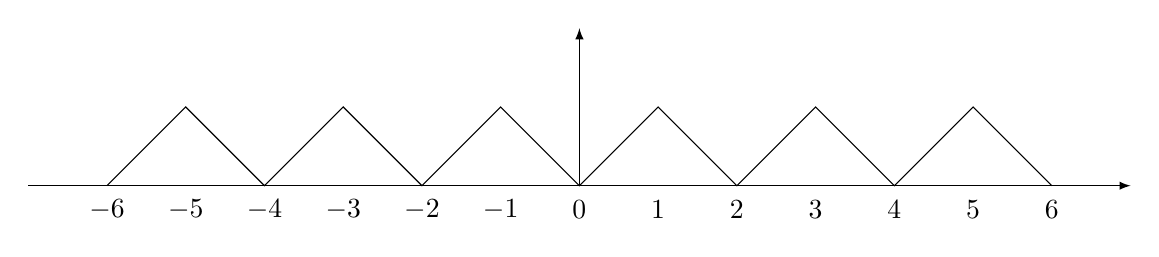
\begin{tikzpicture}
		\draw[-latex] (-7,0) -- (7,0);
		\draw[-latex] (0,0) -- (0,2);
		\draw (-6,0) -- (-5,1) -- (-4,0) -- (-3,1) -- (-2,0) -- (-1,1) -- (0,0) -- (1,1) -- (2,0) -- (3,1) -- (4,0) -- (5,1) -- (6,0);
		\draw (-6,-0.3) node{$-6$};
		\draw (-5,-0.3) node{$-5$};
		\draw (-4,-0.3) node{$-4$};
		\draw (-3,-0.3) node{$-3$};
		\draw (-2,-0.3) node{$-2$};
		\draw (-1,-0.3) node{$-1$};
		\draw (0,-0.3) node{$0$};
		\draw (1,-0.3) node{$1$};
		\draw (2,-0.3) node{$2$};
		\draw (3,-0.3) node{$3$};
		\draw (4,-0.3) node{$4$};
		\draw (5,-0.3) node{$5$};
		\draw (6,-0.3) node{$6$};
	\end{tikzpicture}
	\caption{Graph of $\phi$}
\end{figure}

	Define $f_n(x) = \left(\frac{3}{4}\right)^n \phi(4^n x)$.
	Then $|f_n| \le \left(\frac{3}{4}\right)^n$.
	By Weierstrass M test, $\displaystyle \sum_{n = 0}^\infty f_n$ converges uniformly on $\mathbb{R}$.
	Consider the function $f : \mathbb{R} \to \mathbb{R}$ defined by $\displaystyle f(x) = \sum_{n = 0}^\infty \left(\frac{3}{4}\right)^n \phi(4^n x)$.
	This sum function $f$ is continuous since the convergence is uniform and $f_n$ are all continuous.\\

	Fix a real number $x$ and a positive integer $m$.
	Define $\displaystyle \delta_m = \pm \frac{1}{2}\ 4^{-m}$ such that no integer lies between $4^m x$ and $4^m(x+\delta_m)$.
	This is possible since $|4^m (x+\delta_m) - 4^m x| = |4^m \delta_m| = \frac{1}{2}$.\\

	\begin{commentary}
		The choice of sign of $\delta_m$ is made depending on the value of $4^m x$.
		Suppose $x = 1.1$ and $m = 3$.
		Then $4^m x = 70.4$.
		Now $\delta = \frac{1}{2}\ 4^{-m} = \frac{1}{128}$ so that $4^m(x+\delta_m)= 70.9$.
		Suppose $x = 1.2$ and $m = 3$.
		Then $4^m x = 76.8$.
		Now $\delta = -\frac{1}{2}\ 4^{-m} = -\frac{1}{128}$ so that $4^m(x+\delta) = 76.3$.\\
	\end{commentary}

	Define
	\[\gamma_n = \frac{\phi(4^n(x+\delta_m)) - \phi(4^n x)}{\delta_m} \]

	If $n > m$, then $4^n \delta_m$ is an even integer and $\gamma_n = 0$.\\
	If $n \le m$, then 
	\[ |\gamma_n| = \left|\frac{\phi(4^n(x+\delta_m)) - \phi(4^n x)}{\delta_m} \right| \le \frac{4^n \delta_m }{\delta_m} \le 4^n \]
	since $|\phi(s)-\phi(t)| \le |s-t|$.\\
	In particular, if $n = m$, then
	\[ |\gamma_m| = \left| \frac{\phi(4^m(x+\delta_m))-\phi(4^m x)}{\delta_m} \right| = 4^m \]
	since $|\phi(4^m (x+\delta_m)) - \phi(4^m x)| = |4^m \delta| = \frac{1}{2}$ as there are no integers between $4^m(x+\delta_m)$ and $4^m x$.\\

	From the definition of $\gamma_n$ we have,
	\begin{align*}
	 \left| \frac{f(x+\delta_m) - f(x)}{\delta_m} \right| 
		& = \left| \sum_{n = 0}^m \left( \frac{3}{4} \right)^n \gamma_n \right| \\
		& = \left| 3^m + \sum_{n = 0}^{m-1} \left( \frac{3}{4} \right)^n \gamma_n \right| \\
		& \ge 3^m - \sum_{n = 0}^{m-1} 3^n = \frac{3^m+1}{2}
	\end{align*}
	Therefore, the function $f$ is not differentiable at $x$ since the following limit does not exist as $m \to \infty$.
	\[ \lim_{\delta_m \to 0} \left| \frac{f(x+\delta_m) - f(x)}{\delta_m} \right| \ge \lim_{m \to \infty} \frac{3^m+1}{2} \]
	Since the choice of $x$ is arbitrary, the function $f$ is nowhere differentiable.
\end{proof}

\pagebreak
{\Large Module 4 : Weierstrass Approximation \& Some Special Functions}
\section{Equicontinuous Family of Functions}
\begin{definition}
	Let $\sequence{f_n}$ be a sequence of functions defined on $E$.\\
	{\color{red}
	Sequence $\sequence{f_n}$ is a \textbf{bounded} sequence if every functions in the sequence is bounded.
	\[ \forall n \in N, \exists M \in \mathbb{R} \text{ such that } \forall x \in E, |f_n(x)|<M \]

	Sequence $\sequence{f_n}$ is a \textbf{pointwise bounded} sequence if there exists a function $\phi(x)$ such that $|f_n(x)| < \phi(x)$.
	In other words, sequence $\sequence{f_n}$ is a pointwise bounded sequence if $\sequence{f_n(x)}$ is bounded for every $x \in E$
	\[ \forall x \in E, \exists M \in \mathbb{R} \text{ such that } \forall n \in \mathbb{N}, |f_n(x)| < M \]
	}

	Sequence $\sequence{f_n}$ is a \textbf{uniformly bounded} sequence if there exists a real number $M$ such that $|f_n(x)| < M$ for every $x \in E$ and $n \in \mathbb{N}$.
	\[ \exists M \in \mathbb{R} \text{ such that } \forall x \in E, \forall n \in \mathbb{N}, |f_n(x)| < M \]
\end{definition}
\subsection{Two Problems}
\begin{enumerate}
	\item Whether uniform bounded sequence of uniformly bounded functions have a convergent subsequence ?
		\textbf{NO}.\\
		Sequence $\sequence{f_n}$ where $f_n(x) = \sin nx$ is uniformly bounded.
		But it doesn't have a convergent subseqeunce.
		\begin{proof}
			Suppose $\sequence{\sin nx}$ has a convergent subsequence, say $\sequence{\sin n_kx}$.
			Then by Cauchy criterion, $(\sin n_k x - \sin n_{k+1}x) \to 0$ as $n_k \to \infty$.
			\[ \lim_{n \to \infty} \sin n_k x - \sin n_{k+1}x = 0 \]
			\[ \lim_{n \to \infty} (\sin n_k x - \sin n_{k+1}x)^2 = 0 \]
			By Lebesgue dominated convergence theorem,
			\[ \lim_{n \to \infty} \int_0^{2\pi} (\sin n_kx - \sin n_{k+1}x)^2 dx = \int_0^{2\pi} \lim_{n \to \infty} (\sin n_kx - \sin n_{k+1}x)^2 dx = 0 \]
			However, the integral on the left evaluates $2\pi$ which is a contradiction.
			Clearly, the uniformly bounded sequence $\sequence{\sin nx}$ of continuous functions on compact interval $[0,2\pi]$ does not even imply existence of a subsequence which converges pointwise.
		\end{proof}
	\item Whether every uniformly bounded, convergent sequence has a  uniformly convergent subsequence ?
		\textbf{NO}.\\
		Consider,
		\[ f_n(x) = \frac{x^2}{x^2+(1-nx)^2} \]
		Sequence $\sequence{f_n}$ is a uniformly bounded sequence of functions on compact interval $[0,1]$.
		doesn't have a convergent subsequence.
		\begin{proof}
			Suppose $\sequence{f_n}$ has a convergent subsequence $\sequence{f_{n_k}} \to f$.
			Then $\displaystyle \lim_{n \to \infty} f_{n_k}(x) = f(x)$.
			We have,
			\[ \lim_{n \to \infty} f_n(x) = \lim_{n \to \infty} \frac{x^2}{x^2+(1-nx)^2} = 0 \]
			However,
			\[ \lim_{n \to \infty} f_n \left(\frac{1}{n}\right) = \lim_{n \to \infty} \frac{\left(\frac{1}{n}\right)^2}{\left(\frac{1}{n}\right)^2+0} = 1 \ne 0 = \left(\lim_{n \to \infty} f_n\right)(x) \] 
			Clearly, the sequence of functions $\{ f_n\}$ is a uniformly bounded sequence of continuous functions on a compact interval $[0,1]$.
			Therefore, uniformly bounded, convergent sequence on compact set doesn't necessarily have a uniformly convergenct subsequence.
		\end{proof}
\end{enumerate}

\begin{definition}
	Let $E$ be a subset of a metric space $X$.
	A family $\mathscr{F}$ of complex functions on $E$ is \textbf{equicontinuous} if for any $\varepsilon > 0$, there exists $\delta > 0$ such that $|f(x)-f(y)| < \varepsilon$ whenever $d(x,y) < \delta$ for any $x,y \in E$ and $f \in \mathscr{F}$.
	\[ \forall \varepsilon > 0, \exists \delta > 0 \text{ such that } \forall f \in \mathscr{F}, |f(x)-f(y)| < \varepsilon \text{ whenever } d(x,y) < \delta \]
	\begin{commentary}
		In equicontinuity, the choice of $\delta$ is independent of the choice of $f$.
	\end{commentary}
\end{definition}

\begin{theorem}
	If $\sequence{f_n}$ is a sequence of pointwise bounded, complex functions on countable set $E$, then it has a subsequence $\sequence{f_{n_k}}$ such that $\sequence{f_{n_k}(x)}$ converges for every $x \in E$.
\end{theorem}
\begin{proof}
	Let $E$ be a countable set.
	Let $\sequence{f_n}$ be a sequence of pointwise bounded, complex functions.
	Let $\sequence{x_i}$ be a sequence in $E$.
	Then $\sequence{f_n(x_1)}$ is a bounded sequence of complex numbers.
	By Bolzano-Weierstrass theorem,  $\sequence{f_n(x_1)}$ has a subsequence $S_1$, say $\sequence{f_{1,k}(x_1)}$ which converges at $x_1 \in E$.
	\[ S_1 : f_{1,1}\ f_{1,2}\ f_{1,3} \dots \]

	Consider, the subsequence $\sequence{f_{2,k}(x_2)}$ of the sequence $\sequence{f_n(x_2)}$ with the same values for $k$ as in subsequence $\sequence{f_{1,k}(x_2)}$.
	Again, $\sequence{f_{2,k}(x_2)}$ is a bounded complex sequence.
	And by Bolzano-Weierstrass theorem, $\sequence{f_{2,k}(x_2)}$ has a convergent subsequence $S_2$, say $\sequence{f_{2,k'}(x_2)}$ which is a subsequence of $\sequence{f_2(x_2)}$.
	And more importantly, $S_2$ is a subsequence of $S_1$ such that $S_2$ converges for both $x_1,x_2 \in E$.
	\[ S_2 : f_{2,1}\ f_{2,2}\ f_{2,3} \dots \]

	Continuing like this, we get a sequence of subsequences
	\begin{align*}
		S_1 \quad & : f_{n,1}\quad f_{n,2}\quad f_{n,3}\quad \dots \\
		S_2 \quad & : f_{n,1}\quad f_{n,2}\quad f_{n,3}\quad \dots \\
		 & \dots \\
		S_n \quad & : f_{n,1}\quad f_{n,2}\quad f_{n,3}\quad \dots
	\end{align*}

	Consider the diagonal sequence, $S : f_{1,1}\ f_{2,2}\ f_{3,3} \dots $.
	We know that discarding finitely many first terms won't affect convergence of sequences.
	And for any natural number $n$, we have can obtain a subsequence of $S_n$ by discarding a finite number of first terms from $S$.
	Thus, we have sequence $S$ which converges for $x_1,x_2,\dots,x_n \in E$ since $S_n$ converges.
	Therefore, as $n \to \infty$ we have a convergent subsequence $S$ of $\sequence{f_n}$ which converges for every $x \in E$.
\end{proof}

\begin{theorem}
	Let $K$ be a compact metric space.
	If $\sequence{f_n}$ is a sequence of pointwise bounded, continuous, complex valued functions on $K$ converges uniformly on $K$, then $\sequence{f_n}$ is equicontinuous on $K$.
\end{theorem}
\begin{proof}
	Let $K$ be a compact metric space.
	Let $\varepsilon > 0$.
	Let $\sequence{f_n}$ converges uniformly on $K$.
	Then,
	\[ \forall \varepsilon > 0,\ \exists N \in \mathbb{N} \text{ such that } \forall n > N,\ \forall x \in K,\ \| f_n(x)-f_N(x) \| < \varepsilon \]

	We have continuous functions on compact sets are uniformly continuous.
	Thus for any $\varepsilon > 0$ there exist $\delta > 0$ such that $|f_j(x) - f_j(y)| < \varepsilon$ whenever $d(x,y) < \delta$.
	Thus, $|f_N(x) - f_N(y)| \le \varepsilon$.\\

	Let $1 \le j \le N$.
	Since the continuity is uniform, there exists $\delta > 0$ such that $|f_j(x) - f_j(y)| < \varepsilon$.\dag\footnote{
		For each functions $f_j$, given $\varepsilon > 0$, there exists $\delta_j > 0$ satisfying the $\varepsilon$-$\delta$ condition for uniform continuity.
		Define $\delta = \min \{ \delta_j : j = 1,2,\dots,N \}$, then for this $\delta$ the condition is satified by functions $f_1,f_2,\dots,f_N$.}\\

	Let $n > N$ and $d(x,y) < \delta$.
	Then,
	\[ |f_n(x)-f_n(y)| \le |f_n(x)-f_N(x)| + |f_N(x) - f_N(y)| + |f_N(y) - f_n(y)| < 3\varepsilon \]

	Therefore, for any $\varepsilon > 0$ there exists $\delta > 0$ such that $\forall n \in \mathbb{N},\ |f_n(x) - f_m(x)| < \varepsilon$ whenever $d(x,y)< \delta$.
	\[ \forall \varepsilon > 0,\ \exists \delta > 0,\ \forall n \in \mathbb{N},\!\! \underset{d(x,y) < \delta}{\forall} \!\!\!\! y \in K,\ |f_n(x)-f_n(y)| < \varepsilon \]
	That is, the sequence $\sequence{f_n}$ is equicontinuous on $K$.
\end{proof}

\begin{theorem}
	Let $K$ a compact.
	If $\sequence{f_n}$ be a sequence of pointwise bounded, equicontinuous, complex functions on $K$, then
	\begin{enumerate}
		\item $\sequence{f_n}$ is uniformly bounded on $K$.
		\item $\sequence{f_n}$ has a uniformly convergent subsequence.
	\end{enumerate}
\end{theorem}
\begin{proof}
	Let $\sequence{f_n}$ be sequence of point-wise bounded, equicontinuous, complex functions on compact set $K$.
	Since $f_n$ are equicontinuous, given $\varepsilon > 0$, there exists $\delta > 0$ such that $\forall n \in \mathbb{N},\ |f_n(x)-f_n(y)| < \varepsilon$ whenever $d(x,y) < \delta$.\\

	Let $\mathcal{C}$ be a cover of $K$ of open balls of radius $\delta$.
	Since, $K$ is compact this cover has a finite subcover, say open balls with center $p_j,\ j = 1,2,\dots,r$.
	Thus there exists finitely many points, $p_j$ such that every point in $K$ is sufficiently close one of them.
	Then for any $x \in K$, there exists some $p_j$ such that $d(x,p_j) < \delta$.\\

	Since $\sequence{f_n}$ is point-wise bounded, there exists $M_j$ such that $|f_n(p_j)| < M_j$.
	Define $M = \max \{ M_1, M_2, \dots, M_r\}$. 
	Then 
	\begin{align*}
		|f_n(x)| & = |f_n(x)-f_n(p_j)+f_n(p_j)| \\
		& \le |f_n(x) - f_n(p_j)| + |f_n(p_j)| \\
		& \le \varepsilon + M
	\end{align*}
	Therefore, $\sequence{f_n}$ is uniformly bounded.\\

	\hrule \vspace{1em}

	Let $\varepsilon > 0$.
	Choose $\delta > 0$ such that $|f_n(x)-f_n(y)| < \varepsilon$ whenever $d(x,y) < \delta$.
	Since $K$ is compact, $K$ has a countable dense subset, say $E = \{x_1,x_2,\dots\}$.
	That is, given $\delta > 0$, for any $x \in K$, there exists $x_j \in E$ such that $d(x,x_j) < \delta$.
	Clearly, $K$ has a cover of open balls with center $x_j$s and radius $\delta$.
	Since $K$ is compact, there exists finitely many points $x_1,x_2,\dots,x_m \in E$ such that $d(x,x_m) < \delta$.\\

	Since $E$ is countable and $\sequence{f_n}$ is point-wise bounded, $\sequence{f_n}$ on $E$ has a subsequence, say diagonal sequence $f_{n_i} = g_i$ which converges for any $x_j \in E$.
	Thus, by Cauchy criterion there exists integer $N$ such that 
	\[ \forall i,j \ge N,\ |g_i(x_s) - g_j(x_s)| < \varepsilon,\quad s = 1,2,\dots,m \]

	Let $x \in K$.
	Let $x_s \in E$ such that $d(x,x_s) < \delta$.
	Then,
	\[ |g_i(x) - g_j(x)| \le |g_i(x)-g_i(x_s)| + |g_i(x_s) - g_j(x_s)| + |g_j(x_s) - g_j(x)| \le 3\varepsilon \]
	That is, $\sequence{g_i}$ is uniformly convergent on $K$.
	Therefore, $\sequence{f_n}$ has a uniformly convergent subseqeunce $\sequence{f_{n_k}}$.
\end{proof}

\begin{theorem}[Weierstrass' Theorem]
	If $f$ is a continuous, complex function on $[a,b]$, there exists a sequence of polynomials $P_n$ such that
	\[ \lim_{n \to \infty} P_n(x) = f(x) \]
	uniformly on $[a,b]$.
	If $f$ is real, the $P_n$ may be taken real.
\end{theorem}
\begin{important}
In other words, any continuous function has a polynomial approximation.
\end{important}
\begin{proof}
	Without loss of generality, suppose $[a,b] = [0,1]$ and $f(0) = f(1) = 0$.\\

	\textbf{Step 1 : WLoG $f(0) = f(1) = 0$}
	\begin{commentary}
	If theorem is true for continuous functions satisfying $f(0) = f(1) = 0$, then it is true for any continuous function.\\
	\end{commentary}

	Let $f$ be any continuous function on $[0,1]$.
	Then there exists a function $g : [0,1] \to \mathbb{R}$ be defined by,
	\[ g(x) = f(x)-f(0) - x[f(1) - f(0)] \]
	such that $g(0) = g(1) = 0$.
	Suppose $g$ can be expressed as limit function of a uniformly convergent sequence of polynomials, say $P_n$.
	We have,
	\[ (f-g)(x) = x[f(1) - f(0)] + f(0) \]
	is a polynomial, say $P(x)$.
	Then $P_n+P \to f$ uniformly as $n \to \infty$, since $P_n \to g$ uniformly and $P$ is a constant polynomial independent of $n$.
	\[ \lim_{n \to \infty} (P_n+P)(x) = \lim_{n \to \infty} P_n(x) + P(x) = g(x) + (f-g)(x) = f(x) \]
	Therefore, it is enough to prove the theorem is true for any continuous function $f$ satisfying $f(0) =f(1) = 0$.\\

	\hrule \vspace{1em}

	\textbf{Step 2 : Construction of $P_n(x)$}\\
	Since $f$ is continous in $[0,1]$, $f$ is uniformly continuous in $[0,1]$.
	Extend $f$ such that $f(x) = 0, \ \forall x \notin [0,1]$.
	Then,  $f$ is uniformly continuous on $\mathbb{R}$.
	Define $Q_n(x) = c_n(1-x^2)^n$ such that
	\[ \int_{-1}^1 Q_n(x) \ dx = 1 \]
	Then we have,
	\begin{align*}
		\int_{-1}^1 (1-x^2)^n \ dx 
		& = 2\int_0^1 (1-x^2)^n \ dx \ \text{ since } (1-x^2)^n \text{ is even} 
		\intertext{We have, Bernouli's inequality. $(1+x)^r \ge (1+rx),\ \forall x \ge -1,\ \forall r \ge 0$}
		\int_{-1}^1 (1-x^2)^n \ dx 
		& \ge 2\int_0^{1/\sqrt{n}} (1-nx^2) \ dx \\
		& \ge 2 \left(\frac{1}{\sqrt{n}} - \frac{n}{3n\sqrt{n}} \right) = \frac{4}{3\sqrt{n}} > \frac{1}{\sqrt{n}}
	\end{align*}
	Clearly, $c_n < \sqrt{n}$. \\

	For $\delta > 0$, $Q_n(x) \le \sqrt{n}(1-\delta^2)^n$ for $\delta \le |x| \le 1$.	
	Then $Q_n \to Q$ uniformly for all such that $\delta \le |x| \le 1$.
	Define $P_n : [0,1] \to \mathbb{R}$ defined by 
	\[ P_n(x) = \int_{-1}^1 f(x+t) \ Q_n(t) \ dt \]
	Then,
	\begin{align*}
		P_n(x) & = \int_{-1}^1 f(x+t) \ Q_n(t) \ dt \\
		& = \int_{-x}^{1-x} f(x+t) \ Q_n(t) \ dt \text{ since } f \text{ vanishes outside } [0,1]\\
		& = \int_0^{1} f(t) \ Q_n(t-x) \ dt 
	\end{align*}
	{\color{red}
	Continuous function $f$ is uniformly continuous on compact interval $[0,1]$.
	Thus $f$ is Riemann integrable on $[0,1]$.
	And $Q_n(t-x) = c_n [1-(t+x)^2]^n$.
	From integration by parts, we know that $\sequence{P_n}$ is a sequence of polynomials.
	\begin{align*}
		P_n(x) 
		& = \int_0^1 f(t) Q_n(t+x) dt \\
		& = \left[f(t)Q_n'(t+x)\right]_0^1 - \int_0^1 Q_n'(t+x) \int_0^1 f(t) dt\\
		& = f(1)Q_n'(1+x) -f(0)Q_n'(x) - [F(1)-F(0)]\int_0^1 Q_n'(t+x) dt \\
		& = f(1)Q_n'(1+x) - f(0)Q_n'(x) - [F(1)-F(0)] [Q_n(1+x) - Q_n(x)]
	\end{align*}
	}
	And for each natural number $n$, we have $P_n(x)$ is real, if $f$ is real.\\

	\hrule \vspace{1em}

	\textbf{Step 3 : $P_n \to f$ uniformly}\\
	Let $\varepsilon > 0$.
	Since extended $f$ is uniformly continuous on real line, there exists $\delta > 0$ such that $|f(y)-f(x)| < \frac{\varepsilon}{2}$ whenever $|y-x| < \delta$.
	\begin{align*}
		|P_n(x)-f(x)| 
		& = \left| \int_{-1}^1 f(x+t)Q_n(t)\ dt - f(x)\int_{-1}^1 Q_n(t)\ dt \right| \\
		& \le \int_{-1}^1 |f(x+t)-f(x)| Q_n(t)\ dt 
		\intertext{Let $M =\sup f(x)$. Then $|f(x+t)-f(x)| \le 2M$. And we have an upper bound for the value $Q_n(x)$ for $\delta \le |x| \le 1$. Therefore, we split the domain of integral into three parts so that we may apply uniform continuity on the middle part and bound of $Q_n$ on other two parts.}
		|P_n(x)-f(x)| 
		& \le 2M \int_{-1}^{-\delta} Q_n(t)dt + \frac{\varepsilon}{2} \int_{-\delta}^{\delta} Q_n(t)dt+2M\int_{\delta}^1 Q_n(t)dt 
		\intertext{We have an upper bound for $Q_n$, say $Q_n(x) \le \sqrt{n}(1-\delta^2)^n$ for $\delta \le |x| \le 1$.}
		|P_n(x)-f(x)| 
		& \le 2M\sqrt{n}(1-\delta^2)^n \int_{-1}^{-\delta} dt + \frac{\varepsilon}{2} \int_{-\delta}^{\delta} Q_n(t)dt+2M \sqrt{n} (1-\delta^2)^n \int_{\delta}^1 dt \\
		& \le 4M\sqrt{n}(1-\delta^2)^n + \frac{\varepsilon}{2} \quad \text{ since } 2(1-\delta) < 2 \\
		& \le \varepsilon \text{ for sufficiently large n}
	\end{align*}
	Therefore, there exists $N \in \mathbb{N}$ such that $\forall n > N,\ |P_n(x) - f(x)| < \varepsilon$.
	In other words, $P_n \to f$ uniformly on $[0,1]$. 
\end{proof}

\begin{corollary}
	For every interval $[-a,a]$ there is a sequence of real polynomials $P_n$ such that $P_n(0) = 0$ and
	\[ \lim_{n \to \infty} P_n(x) = |x| \]
	uniformly on $[-a,a]$.
\end{corollary}
\begin{proof}
	By Weierstrass theorem, there exists a sequence $\sequence{P_n^\ast(x)}$ of real polynomials which converges to $|x|$ uniformly on $[-a,a]$.
	Thus, $P_n^\ast(0) \to 0$ as $n \to \infty$.
	Define $P_n(x) = P_n^\ast(x) - P_n^\ast(0)$.
	Clearly, $P_n(0) = 0$ and the sequence $\sequence{P_n(x)}$ converges uniformly on $[-a,a]$.
	And,
	\[ \lim_{n \to \infty} P_n(x) = \lim_{n \to \infty} P_n^\ast(x) - \lim_{n \to \infty}P_n^\ast(0) = |x| \]	
	Therefore, $P_n(0) = 0$ and $P_n(x) \to |x|$ as $n \to \infty$.
\end{proof}

\begin{remark}[Out of Syllabus]
	On the other side of this corollary, we have Stone-Weierstrass theorem which study functions that doesn't vanish anywhere.\\

	Let $\mathscr{A}$ be an algebra of functions defined on compact set $K$ that separates points and vanishes nowhere.
	By Stone-Weierstrass theorem,\dag\footnote{
		\cite[\S7.32]{rudin} Let $\mathscr{A}$ be a family of functions defined on compact set $K$.\\
		$\mathscr{A}$ separates points if $\forall x \in K,\ \exists f,g \in \mathscr{A}$ such that $f(x) \ne g(x)$.\\
		$\mathscr{A}$ vanishes at a point $x \in K$ if $\forall x \in K,\ \exists f \in \mathscr{A}$ such that $f(x) \ne 0$ }
	any continuous function $f$ on $K$  has a sequence of functions in $\mathscr{A}$ which converges to $f$ uniformly on $K$.
	The algebra of even polynomials doesn't separate points since $P_n(x) = P_n(-x)$.
\end{remark}

%\chapter{Weierstrass Approximation \& Some Special Functions
\subsection{Some special functions}
\begin{definition}[analytic function]
	A function $f$ is (real) analytic if it can be represented by a power series.
	\[ f(x) = \sum_{j=1}^\infty c_n x^n \]
\end{definition}

\begin{remark}
	The open interval in which a power series $\sum c_n x^n$ converges is the \textbf{interval of convergence}.
\end{remark}

\begin{theorem}
	Suppose series $\sum c_n x^n$ converges for $|x| < R$.
	Suppose function $f : (-R,R)$ is defined by \[ f(x) = \sum_{n = 0}^\infty c_n x^n,\ |x| < R \]
	Then,for any $\varepsilon > 0$, the series $\sum c_n x^n$ converges uniformly on $[-R+\varepsilon,R-\varepsilon]$.
	Also the function $f$ is continuous and differentiable in $(-R,R)$ and
	\[ f'(x) = \sum_{n = 1}^\infty nc_n x^{n-1},\quad |x| < R \]
\end{theorem}
\begin{proof}
	Let $\varepsilon > 0$.
	Then for $|x| \le R - \varepsilon$ we have $|c_n x^n| \le |c_n (R-\varepsilon)^n|$.\\

	We have, 
	\[ \limsup_{n \to \infty} |R-\varepsilon| \sqrt[n]{|c_n|} = (R-\varepsilon) \limsup_{n \to\infty} \sqrt[n]{|c_n|} = 0 < 1 \]

	By raio test, the series $\sum c_n (R-\varepsilon)^n$ converges absolutely.
	By Weierstrass M test, series $\sum c_n x^n$ converges uniformly on $[-R+\varepsilon,R-\varepsilon]$.
	In the same fashion, the series $\sum nc_n x^{n-1}$ converges uniformly on $[-R+\varepsilon,R-\varepsilon]$ since $\displaystyle \limsup_{n \to \infty} \sqrt[n]{n|c_n|} = 0$.\\

	Let $x_0 \in (-R,R)$.
	Then there exists $\varepsilon > 0$ such that $x_0 \in [-R+\varepsilon, R-\varepsilon]$.
	The series $\sum n c_n x^{n-1}$ converges to $f'(x)$ uniformly on $[-R+\varepsilon,R-\varepsilon]$ and $f(x_0) = \sum c_n x_0^n$.
	Thus, $f$ is differentiable on $[-R+\varepsilon,R-\varepsilon]$ and
	\[ f'(x) = \lim_{n \to \infty} \sum_{k=1}^n k c_k x^{k-1} = \sum_{n = 1}^\infty n c_n x^{n-1} \]
	We know that $f$ is continuous at a point if it is differentiable at that point.
	Thus, $f$ is continuous on $[-R+\varepsilon,R-\varepsilon]$.
\end{proof}

\begin{corollary}
	Suppose $\displaystyle \sum_{n = 0}^\infty c_n x^n$ converges for $|x| < R$ and function $f$ is defined by $f(x) = \displaystyle \sum_{n = 0}^\infty c_n x^n$.
	Then $f$ has derivatives of all ordres, say $f^{(k)}(x)$ given by
	\[ f^{(k)}(x) = \sum_{n=k}^\infty n(n-1)\dots(n-k+1)c_n x^{n-k} \]
	In particular,
	\[ f^{(k)}(0) = k!\ c_k \]
\end{corollary}
\begin{proof}
	Let $f(x) = \sum c_n x^n$.
	Then, we have 
	\[ f'(x) = \sum_{n = 1}^\infty n c_n x^n \]
	By mathematical induction, we have
	\[ f^{(k)}(x) = \sum_{n = k}^\infty n(n-1)\dots(n-k+1) c_n x^{n-k} \]
	When $x = 0$, we get
	\[ f^{(k)}(0) = \sum_{n = k}^\infty n(n-1)\dots(n-k+1) c_n 0^{n-k} = {\color{red}k!\ c_k} \]
\end{proof}

\begin{theorem}
	Suppose $\displaystyle \sum_{n = 0}^\infty c_n$ converges.
	Define \[ f(x) = \sum c_n x^n,\quad -1<x<1 \]
	Then,
	\[ \lim_{x \to 1} f(x) = \sum_{n=0}^\infty c_n \]
\end{theorem}
\begin{proof}
	Let $s_n = c_0 + c_1 + \dots + c_n$ and $s_{-1} = 0$.
	Suppose $\sum c_n$ converges, then $s_n$ converges, say $s_n \to s$.
	Let $\varepsilon > 0$.
	Then there exists $N \in \mathbb{N}$ such that $\forall n > N,\ |s-s_n| < \frac{\varepsilon}{2}$.\\

	Also we have,
	\begin{align*}
		\sum_{n=0}^m c_n x^n
		& = \sum_{n=0}^m (s_n-s_{n-1})x^n \\
		& = \sum_{n=0}^m s_n x^n - xs_{n-1}x^{n-1} \\
		& = \sum_{n=0}^m s_nx^n - x\sum_{n=0}^{m}s_{n-1}x^{n-1} \\
		& = \sum_{n=0}^m s_nx^n - x\sum_{n=-1}^{m-1}s_nx^n \\
		& = \sum_{n=0}^{m-1} s_nx^n + s_mx^m - x\sum_{n=0}^{m-1}s_nx^n \text{ since $s_{-1} = 0$} \\
		& = (1-x)\sum_{n=0}^{m-1} s_nx^n + s_mx^m \\
		\lim_{m \to \infty} \sum_{n=0}^m c_n x_n
		& = (1-x) \lim_{m \to \infty} \sum_{n=0}^{m-1} s_nx^n + \lim_{m \to \infty} s_m x^m  \\
		f(x) & = (1-x) \sum_{n=0}^\infty s_nx^n \text{ since $s_m \to s$, $|x|<1$ and $x^m \to 0$}
	\end{align*}

	{\color{red}
	We know that,
	\[ (1-x)\sum_{n=0}^m x^n = (1-x)(1+x+x^2+\dots+x^m) = 1-x^{m+1} \]
	Thus,
	\[ \lim_{m \to \infty} (1-x)\sum_{n=0}^m x^n = \lim_{m \to \infty} 1-x^{m+1} = 1 \]
	}
	Thus,
	\begin{align*}
		|f(x) - s| 
		& = \left| (1-x)\sum_{n=0}^\infty s_nx^n - s(1-x)\sum_{n=0}^\infty x^n \right| \\
		& = (1-x) \left| \sum_{n=0}^\infty (s_n-s)x^n \right| \\
		& \le (1-x) \sum_{n=0}^\infty |(s_n-s)x^n| \\
		& \le (1-x)\sum_{n=0}^\infty |s_n-s|\ |x|^n  \\
		& {\color{red}\le (1-x)\sum_{n=0}^N |s_n-s|\ |x|^n +  \frac{\varepsilon}{2} (1-x) \sum_{n=N+1}^\infty x^n} \\
	\end{align*}
	{ \color{red}
	Let $1-x < \delta < 1$.\dag\footnote{
		In earlier version, the term $|s_n-s|$ was neglected.
		Corrected as per the seminar by Haripriya}
	\[ \lim_{x \to 1} |f(x) - s| \le \lim_{\delta \to 0} \delta \sum_{n=0}^N |s_n -s| (1-\delta)^n + \frac{\varepsilon}{2} = 0 \]
	}	
	Therefore, 
	\[ f(1) = \lim_{x \to 1} f(x) = s = \sum_{n = 0}^\infty c_nx^n \]
\end{proof}

\begin{theorem}
	Given a double sequence $\sequence{a_{ij}}$.
	Suppose that,
	\[ \sum_{j=1}^\infty |a_{ij}| = b_i \]
	and $\sum b_i$ converges.
	Then,
	\[ \sum_{i=1}^\infty \sum_{j=1}^\infty a_{ij} = \sum_{j=1}^\infty \sum_{i=1}^\infty a_{ij} \]
\end{theorem}
\begin{proof}
	\textbf{Step 1 : Construction of $f_i$}\\
	Given series $\displaystyle \sum_{j=1}^\infty |a_{ij}|$ converges to $b_i$.
	Let $E = \{ x_0,x_1,x_2,\dots \}$ be a countable set such that $x_n \to x_0$ as $n \to \infty$.
	Define sequence of functions $\sequence{f_i}$ on $E$ such that 
	\[ f_i(x_n) = \sum_{j=1}^n a_{ij},\ \forall n \in \mathbb{N} \quad \text{ and } \quad f_i(x_0) = \sum_{j=1}^\infty a_{ij} \]
	Clearly, $f_i(x_0) = b_i$ and $f_i(x_n) \to f_i(x_0)$ as $n \to \infty$.\\

	\textbf{Step 2 : $f_i$ is continuous at $x_0$}\\
	We have, $f_i(x_n) \to f_i(x_0)$.
	{\color{red}Then \dag\footnote{
		The method of contradiction was an unnecessary complication.
		Corrected as per the seminar by Mekha},
	\[ \lim_{x_n \to x_0} f_i(x_n) = \lim_{n \to \infty} \sum_{i=1}^n a_{ij} = \sum_{i=1}^\infty a_{ij} = f_i(x_0) \]
	}
	Therefore, function $f_i$ is continuous at $x_0$.\\

	\textbf{Step 3 : Construction of $g$}\\
	Given $|f_i(x)| < b_i$ and $\sum b_i$ converges.
	Thus, $\sum f_i(x)$ converges.
	Define $g : E \to \mathbb{R}$ such that
	\[ g(x) = \sum_{i = 1}^\infty f_i(x) \]
	Since $f_i$ are continuous functions defined on a countable set $E$, the convergence is uniform and the sum $g$ is continuous.
	And we have,
	\[ \lim_{n \to \infty} \lim_{m \to \infty} \sum_{i=1}^m f_i(x_n) = \lim_{x_n \to x_0} g(x_n) = g(x_0) = \lim_{m \to \infty} \sum_{i=1}^m f_i(x_0) = \lim_{m \to \infty} \lim_{n \to \infty} \sum_{i = 1}^m f_i(x_n) \]
	{\color{red}
	Therefore,
	\[ \sum_{i=1}^\infty \sum_{j=1}^\infty a_{ij} = \sum_{j=1}^\infty \sum_{i=1}^\infty a_{ij} \]
	}
\end{proof}

\begin{theorem}[Taylor]
	Suppose $f(x) = \sum c_n x^n$, the series converging in $|x| < R$.
	If $-R < a < R$, then $f$ can be expanded in a power series about the point $x = a$ which converges in $|x-a| < R-|a|$.
	And,
	\[ f(x) = \sum_{n = 0}^\infty \frac{f^{(n)}(a)}{n!} (x-a)^n,\quad |x-a| < R-|a|\]
\end{theorem}
\begin{proof}
	Suppose 
	\begin{align*}
		f(x)
		& = \sum_{n=0}^\infty c_n[(x-a)+a]^n \\
		& = \sum_{n=0}^\infty c_n \sum_{m=0}^n  \binom{n}{m} a^{n-m}(x-a)^m 
		%& = \lim_{k \to \infty} \sum_{n=0}^k c_n \sum_{m=0}^n  \binom{n}{m} a^{n-m}(x-a)^m 
		\intertext{Changing the order of summation, we may combine coefficients of $(x-a)^m$.}
		%& = \lim_{k \to \infty} \sum_{m=0}^k \sum_{n = m}^k \binom{n}{m} c_n a^{n-m} (x-a)^m \\
		& = \sum_{m=0}^\infty \sum_{n = m}^\infty \binom{n}{m} c_n a^{n-m} (x-a)^m
	\end{align*}

	Therefore, it is enough to prove that the order of summation can be changed.
	We know that the order of summation can be changed if,
	\[ \sum_{n = 0}^\infty \sum_{m = 0}^n \left| c_n \binom{n}{m} a^{n-m} (x-a)^m \right| \text{ converges} \]
	We know that,
	\[ \sum_{n = 0}^\infty \sum_{m = 0}^n \left| c_n \binom{n}{m} a^{n-m} (x-a)^m \right| = \sum_{n = 0}^\infty |c_n|\ (|x-a|+|a|)^n \]
\end{proof}
	and it converges if $|x-a|+|a| < R-|a|$.\\

	Also we know that, if $f(x) = \sum c_n x^n$ converges in $|x|<R$, then the convergence is uniform in $[-R+\varepsilon,R-\varepsilon]$ and it is differentiable in $(-R,R)$.
	And the derivatives are given by,
	\[ f^{(m)}(a) = \sum_{n=m}^\infty \frac{n!}{(n-m)!}c_n a^{n-m} = m! \sum_{n=m}^\infty \binom{n}{m} c_n a^{n-m} \]
	Thus,
	\[ f(x) = \sum_{m = 0}^\infty \sum_{n = m}^\infty c_n\binom{n}{m} a^{n-m} (x-a)^m = \sum_{m=0}^\infty \frac{f^{(m)}(a)}{m!}(x-a)^m \]

\begin{theorem}
	Suppose the series $\sum a_n x^n$ and $\sum b_n x^n$converge in the segment $S = (-R,R)$.
	Let $E$ be the set of all $x \in S$ at which
	\[ \sum_{n = 0}^\infty a_n x^n = \sum_{n = 0}^\infty b_n x^n \]
	If $E$ has a limit point on $S$, then $a_n = b-n$.
\end{theorem}
\begin{important}
	In other words, If two power series coverges to the same function in $(-R,R)$, then the series are identical.
\end{important}
\begin{proof}
\end{proof}

\begin{doubt}
Whether the power series representation is unique ?
\end{doubt}

\begin{theorem}
	Let $e^x$ be defined on $\mathbb{R}$.
	Then
	\begin{enumerate}
		\item $e^x$ is continuous and differentiable for all $x$.
		\item $(e^x)' = e^x$
		\item $e^x$ is a strictly increasing function
		\item $e^{x+y} = e^x e^y$
		\item $e^x \to +\infty$ as $x \to \infty$ an d $e^x \to 0$ as $x \to \infty$ and $e^x \to 0$ as $x \to -\infty$
		\item $\displaystyle \lim_{x \to \infty} x^ne^{-x} = 0$ for every $n$.
	\end{enumerate}
\end{theorem}
\begin{proof}
\end{proof}

\begin{theorem}
	\begin{enumerate}
		\item The function $E$ is periodic with period $2\pi i$.
		\item The functions $C$ and $S$ are periodic with period $2\pi i$.
		\item If $0 < t < 2\pi$, then $E(it) \ne 1$.
		\item If $z$ is a complex number with $|z| =1$, there is a unique $t \in [0,2\pi]$ such that $E(it) = z$.
	\end{enumerate}
\end{theorem}
\begin{proof}
\end{proof}

\begin{theorem}
	Suppose $a_0,a_1,\dots,a_n$ are complex numbers.
	\[ P(z) = \sum_{n=0}^\infty a_k z^k \]
	Then $P(z) = 0$ for some complex number $z$.
\end{theorem}
\begin{proof}
\end{proof}



\chapter{Graph Theory}
%Text Books : \cite{balakrishnan}
%Module I:
%Introduction, Basic concepts. Sub graphs. Degrees of vertices. Paths and Connectedness, Automorphism of a simple graph, line graphs, Operations on graphs, Graph Products.
%Directed Graphs : Introduction, basic concepts and tournaments.
%(Chapter 1 Sections 1.1 – 1.7( Upto 1.7.3 including ) 1.8, 1.9)
%(Chapter 1 Sections 2.1, 2.2, 2.3) (20Hours)
%Module II:
%Connectivity : Introduction, Vertex cuts and edge cuts, connectivity and edge connectivity, blocks, Cyclical edge Connectivity of a graph.
%Trees; Introduction, Definition, characterization and simple properties, centres and cancroids, counting the number of spanning trees, Cayley’s formula.
%Applications
%(Chapter 3 Sections 3.1, 3.2 , 3.3, 3.4 and 3.5 )
%(Chapter 4 Sections4.1, 4.2, 4.3, 4.4 (Up to 4.4.3 including ) and 4.5, 4.7) (25Hours)
%Module III:
%Eulerian and Hamiltonian Graphs: Introduction, Eulereian graphs,
%Hamiltonian Graphs, Hamiltonian around’ the world’ game
%Graph Colorings: Introduction, Vertex Colorings, Applications of Graph Coloring, Critical Graphs, Brooks’ Theorem
%(Chapter 6 Sections 6.1, 6.2 and 6.3 )
%(Chapter 7 Sections 7.1, 7.2 and7.3(Up to 7.3.1 including ) (20Hours)
%Module IV:
%Planarity: Introduction, Planar and Nonplanar Graphs, Euler Formula and Its Consequences, K5 and K 3,3 are Nonplanar Graphs, Dual of a Plane Graph, The Four-Color Theorem and the Heawood Five-Color Theorem .
%Spectral Properties of Graphs: Introduction, The Spectrum of a Graph, Spectrum of the Complete Graph Kn, Spectrum of the Cycle Cn,
%(Chapter 8 Sections 8.1, 8.2 , 8.3, 8.4, 8.5 and 8.6 )
%(Chapter 11 Sections 11.1, 11.2 , 11.3 and 11.4) (25Hours)

%Module 1 - \cite{balakrishnan} 1, 2
%Module 2 - \cite{balakrishnan} 3, 4
%Module 3 - \cite{balakrishnan} 6, 7
%Module 4 - \cite{balakrishnan} 8, 11
%Missing - \cite{balakrishnan} 5, 9, 10, ?

%\chapter{Basic Results}
\section{Basic Results}
\subsection{Introduction}
\cite{balakrishnan}
\subsection{Basic Concepts}
\begin{definition}
	A \textbf{graph} is an ordered triple $G = (V,E,I)$ where $V$ is a nonempty set of vertices, $E$ is a set of edges and $I$ is an incidence map which associates each edge with an unordered pair of vertices.
\end{definition}

\begin{description}
	\item[end vertices] Let $e$ be an edge with $I_G(e) = \{ u,v \}$. Then $u,v$ are the end vertices of $e$. We may write $e = uv$.
	\item[incident] An edge $e =uv $ said to be incident on both vertices $u$ and $v$. Then vertices $u$ and $v$ are incident on edge $e$ as well. 
	\item[parallel edges] are those edges which have same pair of end vertices.
	\item[loop] is an edge whose both end vertices are the same.
	\item[neighbour] Vertex $u$ is neighbour of vertex $v$ if $uv$ is an edge of the graph.
	\item[Open neighbourhood] $N(u)$ is the set of all neighbours of the vertex $u$.
	\item[Closed neighbourhood] $N[u] = N(u) \cup \{ u \}$.
	\item[simple] graph does not have any parallel edges or loops.
	\item[adjacent] Two vertices $u,v$ are adjacent if both $u,v$ are incident on an edge, say $uv$. Two edges are adjacent if they have a common end vertex.
\end{description}
\begin{definition}
	A graph is \textbf{finite} if both vertex set $V$ and edge set $E$ are finite. A finite graph, $G$ order, $n(G) = |V(G)|$ and size, $m(G) = |E(G)|$. Or simply $n = |V(G)|$ and $m = |E(G)|$.
\end{definition}

\begin{definition}
	A graph $G$ is \textbf{labeled} if its vertices are distinguished from one another by means of distinct labels.
\end{definition}

\begin{definition}
	Two graphs $G$ and $H$ are \textbf{isomorphic} if there exists a pair $(\phi,\theta)$ where $\phi : V(G) \to V(H)$ and $\theta : E(G) \to E(H)$ are bijections such that $I_G(e) = \{ u,v \} \iff I_H(\theta(e)) = \{ \phi(u),\phi(v) \}$.\\

	Two simple graphs $G$ and $H$ are \textbf{isomorphic} if there exists a bijection $\phi : V(G) \to V(H)$ which induced another bijection $\theta : E(G) \to E(H)$ such that $I_G(e) = \{ u,v \} \iff I_H(\theta(e)) = \{ \phi(u),\phi(v) \}$.
\end{definition}

\begin{exercise}
	Let $G$, $H$ be simple graph and let $\phi : V(G) \to V(H)$ be a bijection such that $uv \in E(G) \implies \phi(u)\phi(v) \in E(H)$. Show that $\phi$ is not an isomorphism.
\end{exercise}
	Let $G,H$ be simple graph with bijection $\phi : V(G) \to V(H)$.
	If there exists two vertices $u,v$ which are non-adjacent in $G$, but $\phi(u),\phi(v)$ are adjacent in $H$.
	Then $\phi$ is not an isomorphism.

\begin{definition}
	A simple graph is \textbf{complete} if every pair of distinct vertices are adjacent.
	A complete graph with $n$ vertices is denoted by $K_n$.
	Then $m(K_n) = \binom{n}{2} = \frac{n(n-1)}{2}$.
	A \textbf{totally} disconnected graph has no edges.
	Thus, $0 \le m \le \binom{n}{2}$.
	A graph $G$ is trivial if it has only one vetex and no edges.
\end{definition}

\begin{definition}
	A graph $G$ is \textbf{bipartite} if its vertex set can be partitioned into two nonempty sets $X$ and $Y$ such that every end of $G$ has one end in $X$ and the other end in $Y$. We write $G(X,Y)$ is bipartite with partition $X,Y$.
	A simple, bipartite graph $G(X,Y)$ is \textbf{complete bipartite} if every vertex in $X$ is adjacent to every vertex in $Y$. Let $G(X,Y)$ be a complete bipartite graph with $|X| = p$ and $|Y|=q$, then we write $K_{p,q}$. A graph of the form $K_{1,q}$ is called a \textbf{star}.
\end{definition}

\begin{remark}
	Let $G$ be a complete bipartite graph, $K_{p,q}$.
	Then it has order $n = p+q$ and size $m = pq$.
\end{remark}

\begin{definition}
Let $G$ be a graph. The complement $G^c$ of graph $G$ is the graph with same vertex set. Two vertices $u,v$ of $G^c$ are adjacent if and only if $u,v$ are non-adjacent in $G$.
	$$ V(G^c) = V(G) \quad \& \quad uv \in E(G^c) \iff uv \notin E(G) $$
\end{definition}
\begin{remark}
	We have, $(G^c)^c = G$, since ${uv \in G \iff uv \notin G^c \iff uv \in (G^c)^c}$ and $V(G) = V(G^c) = V((G^c)^c)$.
	Let $G$ be a graph of order $n$, then $E(G) + E(G^c) = E(K_n)$ as each edge of $K_n$ is either an edge of $G$ or an edge of $G^c$.
\end{remark}

\begin{definition}
	A simple graph is self-complementary if $G \cong G^c$.
\end{definition}
\begin{remark}
	The order of a self complementary graph $G$ of order $n$ is $n(n-1)/4$ since $m(G) = m(G^c)$ and $m(G) + m(G^c) = m(K_n)$.
\end{remark}

\subsection{Subgraphs}
\begin{description}
	\item[subgraph] A graph $H$ is a subgraph of $G$ if $V(H) \subset V(G)$, $E(H) \subset E(G)$ and $I_H$ is $I_G$ restricted to $E(H)$. Then $G$ is a \textbf{supergraph} of $H$.
	\item[induced subgraph] Let $G$ be a graph and $S$ be a subset of the vertex set of $G$. The subgraph induced by $S$, $G[S]$ has vertex set $S$ and two vertices are adjacent only if they are adjacent in $G$.
	\item[edge induced subgraph] Let $G$ be a graph and $S$ be a subset of the edge set of $G$. The subgraph induced by the edge set $S$ is denoted by $G[S]$. Vertex $u$ is a vertex of $G[S]$ only if $S$ has an edge incident on it.
	\item[spanning subgraph] Let $H$ be a subgraph of graph $G$. If $V(H) = V(G)$, then $H$ is a spanning subgraph.
	\item[clique] is a subgraph which is complete. A clique is maximal if it is not contained in another clique.
\end{description}

\begin{remark}
	If an edge $e$ is deleted from a graph $G$, then vertex set remains the same. The graph $G-\{e\}$ is a spanning subgraph of $G$.
	If a vertex $u$ is deleted from a graph $G$, then all the edge incident on $u$ are also deleted. The graph $G-\{u\}$ is an induced subgraph of $G$.
\end{remark}

\subsection{Degree of Vertices}
\begin{definition}
	Let $G$ be a graph and $u$ be a vertex of $G$.
	The \textbf{degree} of $u$ is the number of edges incident on it with multiplicities. That is, every loop incident on $u$ is counted twice.
\end{definition}
\begin{remark}
	In a simple graph, the degree of a vertex is the cardinality of its open neighbourhood.
	$\deg_G(u) = |N_G(u)|$.
\end{remark}

\begin{definition}
	A graph $G$ is $k$-\textbf{regular} if every vertex is of degree $k$. Graph $G$ is \textbf{regular} if it is $k$-regular for some $k$. \textbf{Cubic} graphs are the $3$-regular graphs.
\end{definition}
\begin{remark}
	Complete graph $K_{n+1}$ are $n$-regular.
	And complete graphs are the smallest regular graphs.
	$K_4$ is cubic.
	Petersen graph is cubic.
\end{remark}
\begin{figure}
\centering
\scalebox{0.9}{
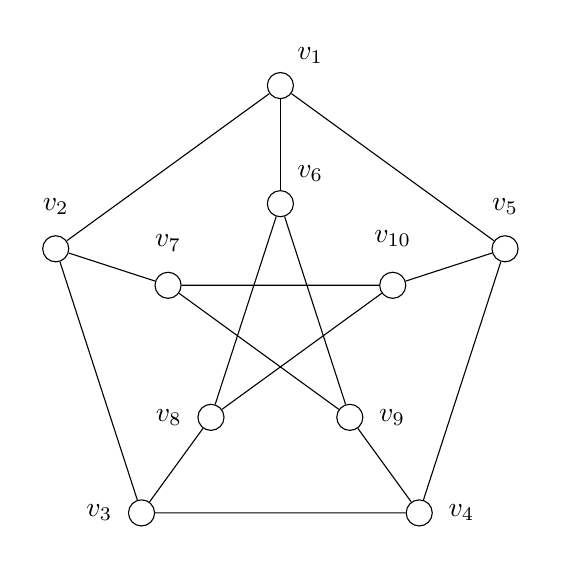
\begin{tikzpicture}
	\node (u){};
	\tikzstyle every node=[draw,circle]
	\draw (u) ++(90:1.5) node (b1)[label=above right:$v_6$]{};
	\draw (u) ++(162:1.5) node (b2)[label=above:$v_7$]{};
	\draw (u) ++(234:1.5) node (b3)[label=left:$v_8$]{};
	\draw (u) ++(306:1.5) node (b4)[label=right:$v_9$]{};
	\draw (u) ++(18:1.5) node (b5)[label=above:$v_{10}$]{};

	\draw (u) ++(90:3) node (a1)[label=above right:$v_1$]{};
	\draw (u) ++(162:3) node (a2)[label=above:$v_2$]{};
	\draw (u) ++(234:3) node (a3)[label=left:$v_3$]{};
	\draw (u) ++(306:3) node (a4)[label=right:$v_4$]{};
	\draw (u) ++(18:3) node (a5)[label=above:$v_5$]{};

	\draw (b1)--(b3)--(b5)--(b2)--(b4)--(b1);
	\draw (a1)--(a2)--(a3)--(a4)--(a5)--(a1);

	\draw (a1)--(b1);
	\draw (a2)--(b2);
	\draw (a3)--(b3);
	\draw (a4)--(b4);
	\draw (a5)--(b5);
\end{tikzpicture}
}
\end{figure}
\begin{remark}
	The complement of a regular graph is also regular. If $G$ is $k$-regular, then $G^c$ is $r$-regular where $k+r = n-1$.
\end{remark}
\begin{description}
	\item[1-factor] is a spanning, $1$-regular subgraph.
	\item[isolated vertex] is a vertex with degree $0$.
	\item[pendent vertex] is a vertex with degree $1$.
	\item[pendent edge] is the only edge incident on a pendent vertex.
\end{description}

\begin{theorem}[Euler]
	The degree sum of a graph is twice its size.
\end{theorem}
\begin{proof}
	Every edge $e= uv$ contributes $1$ to the degree of both the end vertices $u$ and $v$. Thus every edge contributes $2$ to the degree sum. There are $m$ edges, thus degree sum is $2m$.
\end{proof}

\begin{corollary}
	In a grpah $G$, the number of vertices of odd degree is even.
\end{corollary}
\begin{proof}
	Let $G$ be a graph of order $n$.
	Let $V_1,V_2$ be the set of vertices of even,odd degree respectively.
	Then, $\sum d_i = \sum_{v \in V_1} \deg(v) + \sum_{v \in V_2} \deg(v)$.
	The degree sum is even and the first sum on RHS is also even. Thus the second sum should be even. Since, each term in the second sum is an odd integer, there are even number of terms in the second sum. In other words, there are even number of vertices with an odd degree.
\end{proof}
\begin{exercise} 
	If $G \overset{\phi}{\cong} H$, then each pair $u,\phi(u)$ have the same degree.
\end{exercise}
Let $G,H$ be isomorphic graphs.
Let $u$ be a vertex of $G$.
A vertex $v$ is adjacent of $u$ in $G$ if and only if $\phi(v)$ is adjacent to $\phi(u)$ in $H$. Thus, $\deg_G(u) = \deg_H(\phi(u))$.

\begin{remark}
	Clearly, a graph isomorphism preserves adjacency, degree of vertices and neighbourhoods, etc.
	$N_H(\phi(u)) = \{ \phi(v) : v \in N_G(u) \}$.
\end{remark}

\begin{exercise}
	Let $d : d_1,d_2,\dots,d_n$ be the degree sequence of a graph $G$.
	Let $r$ be a positive integer, then $\sum d_i^r$ is even.
\end{exercise}
Let $G$ be a graph of order $n$.
Let $V_1,V_2$ be the set of vertices of even and odd degree respectively.
Clearly, $\sum d_i^r = \sum_{v \in V_1} d_i^r + \sum_{v \in V_2} d_i^r$.
Once again, the first sum on RHS is even as $d_i^r$ is even when $d_i$ is even. And the second sum is odd as $d_i^r$ is odd when $d_i$ is odd. By Euler`s theorem, there are an even number of such odd terms. Thus, the second sum on RHS is also even. Therefore, $\sum d_i^r$ is even.

\begin{definition}
	A sequence of nonnegative integers $d : d_1,d_2,\dots,d_n$ is \textbf{graphical} if there exists a \textit{simple} graph with degree sequence $d$.
\end{definition}

\begin{example}
	The sequence $d : 7,6,3,3,2,1,1,1$ is nongraphical. Let $v_0,v_1$ be the vertics with degree $7,6$ respectively. Then for $d$ to be graphical, there should be at least another $4$ vertices with degree greater than or equal to $2$.
	This is not the case, therefore $d$ is not graphical.
\end{example}

\begin{exercise}
	Let $d : d_1,d_2,\dots,d_n$ is a sequence of nonnegative integers with $\sum d_i$ even. Show that there exists a non-simple graph with $d$ as its degree sequence.
\end{exercise}
	Let $d : d_1,d_2,\dots,d_n$ be a sequence of nonnegative integers with $\sum d_i$ even. Then there are even number of odd integers (if any).\\

	Step 1 : Draw a vertex $u_i$ for each term $d_i$.
	If a pair $(d_i,d_j)$ is odd\footnote{If you want maximal simple graph, you may add an edge $u_iu_j$(if it not already there) and subtract $1$ from both $d_i$ and $d_j$, provided both $d_i$ and $d_j$ are nonzero.}, then draw an edge $u_iu_j$ and subtract $1$ from both $d_i$ and $d_j$.\\

	Step 2 : If $d_i = 2k$. Draw $k$ loops on $u_i$.\\

\begin{challenge}
	Draw maximal connected graph for a degree sequence ?
\end{challenge}

\begin{application}
	In any group of $n$ persons ($n \ge 2$), there are at least two with same number of friends.
\end{application}
\begin{proof}
	Suppose group of $n$ persons is modelled by a graph with $n$ vertices and two vertices are adjacent if the respective persons are friends. It is assumed that friendship is mutual, otherwise it is not considered. Suppose all of them have different number of friends. Then every vertex in the graph has different degree.\\

	The possible degree of a vertex in a graph of order $n$ is $0,1,\dots,(n-1)$. Since all $n$ vertices have different degree and we have only $n$ options. There exists a vertex of degree $j$ for each $0 \le j < n$. This leads to a contradiction.\\

	Let $v_1,v_n$ be the vertices with degree $0,(n-1)$. Then $v_n$ is adjacent to every other vertex and $v_1$ is non-adjacent to every other vertex which is not possible. Thus, at least two vertices should have same degree. Therefore, in a group of $n$ persons, at least two of them have same number of friends.
\end{proof}

\begin{exercise}
	Let $G$ be a graph in which every vertex is of degree $k$ or $k+1$. Then the number of vertices with degree $k$ is $(k+1)n-2m$.
\end{exercise}
\begin{proof}
	Let $G$ be a graph of order $n$ and size $m$.
	Let $x$ be the number of vertices with degree $k$.
	Then there are $n-x$ vertices with degree $k+1$.
	By Euler`s theorem, $ xk + (n-x)(k+1) = 2m \implies x = (k+1)n-2m$.
\end{proof}
	
\subsection{Paths and Connectedness}
\begin{definition}
	Let $G$ be a graph. A \textbf{walk} on $G$ is an alternating finite sequence of vertices and edges which starts and ends at some vertices, say $W : v_0 e_0 v_1 e_1 \dots e_k v_k$.
	The vertex $v_0$ is the \textbf{origin} and $v_k$ is the \textbf{terminus} of the walk $W$.
\end{definition}
\begin{description}
	\item[closed walk] A walk is \textbf{closed} if its origin and terminus are identical. Otherwise the walk is \textbf{open}.
	\item[trail] is a walk in which edges are distinct.
	\item[path] is a trail in which vertices are distinct.
	\item[cycle] is a closed trail in which vertices are distinct.
\end{description}

\begin{remark}
	A walk of length zero is a single vertex. And this walk is called a \textbf{trivial path}.
	Let $P : v_0,e_1,v_1,e_2,v_2,\dots,v_{k-1},e_k,v_k$ be a path in $G$. Then the \textbf{inverse of the path} is given by, $P^{-1} : v_k,e_k,v_{k-1},\dots,v_1,e_1,v_0$.
	And $v_j,e_j,v_{j+1},\dots,v_{k-1},e_{k-1},v_k$ is the $v_j-v_k$ \textbf{section} of the path $P$.
\end{remark}

\begin{definition}
	Let $G$ be a graph. Then connectedness is an equivalence relation on $V(G)$. Let $V_1,V_2,\dots,V_\omega$ be the equivalence classes. Then the induced subgraphs $G[V_1], G[V_2], \dots, G[V_\omega]$ are the \textbf{components} of $G$.
\end{definition}

\begin{remark}
	For a connected graph, $\omega = 1$. And for disconnected graphs $\omega \ge 2$. And components are maximal connected subgraphs of $G$. The number of components of $G$ is denoted by $\omega(G)$.
\end{remark}

\begin{definition}
	Let $d : V(G) \to V(G),\ d(u,v)$ is the length of the shortest $u-v$ path. If there is no $u-v$ path, then $d(u,v) = \infty$.
\end{definition}
\begin{exercise}
	Let $G$ be a simple graph.
	The vertex set $V(G)$ together with distance function $d(u,v)$, length of shortest $u-v$ path is a metric space.
\end{exercise}
\begin{proof}
	Let $G$ be a simple graph with vertex set $V(G)$ and $d : V(G) \to V(G),\ d(u,v)$ is the length of a shortest $u-v$ path.
\begin{enumerate}
	\item Every path has non-negative length. Thus, $\forall u,v \in V(G),\ d(u,v) \ge 0$.\\
	And $d(u,u) = 0$ since trivial path has zero length.
	\item Suppose $u,v$ are connected in $G$. Otherwise $d(u,v) = d(v,u) = \infty$.\\
	Let $P$ be a shortest $u-v$ path. Then $P^{-1}$ is a shortest $v-u$ path.
	Suppose there exists a $v-u$ path, $Q$ which is shorter than $P^{-1}$. Then $Q^{-1}$ is shorter than $P$ which is a contradiction.
	Thus, $d(u,v) = d(v,u)$.
	\item Suppose $d(u,v) < \infty$. Otherwise the result is trivial.\\
	Let $P,Q$ be shortest $u-w$ path, $w-v$ path in $G$. Then $P+Q$ is a $u-v$ walk.
	Thus, there exists a $u-v$ path\footnote{Every $u-v$ walk, contains a $u-v$ path which can be obtained by subsequently replacing each $w-w$ section of the walk with $w$.} of length less than or equal to the length of $P+Q$.
	Therefore, $d(u,v) \le d(u,w) + d(w,v)$.
\end{enumerate}
\end{proof}

\begin{proposition}
	If $G$ is a simple graph with $\delta(G) \ge \frac{n-1}{2}$, then $G$ is connected.
\end{proposition}
\begin{proof}
	Let $G$ be a graph of order $n$.
	Suppose $G$ is not connected. Then $G$ has at least two components, say $G_1$ and $G_2$.
	Let $v \in V(G_1)$. Since $\deg(v) \ge \frac{n-1}{2}$, there are at least $\frac{n-1}{2}$ other vertices in $G_1$.
	Thus, each component of $G$ has at least $\frac{n+1}{2}$ vertices.
	And $G$ has at least $\frac{n+1}{2} + \frac{n+1}{2}$ vertices which is a contradiction.
	Therefore, $G$ is connected.
\end{proof}

\begin{exercise}
	A simple graph with $\delta(G) \ge \frac{n-2}{2}$ is not necessarily connected.
\end{exercise}
\begin{proof}
	Let $G$ be a simple graph with $\delta(G) = \frac{n-2}{2}$ where $n$ is even. Then $G$ is not necessarily connected. For example, $2K_2$ has $\delta = 1$ and is disconnected.
\end{proof}

\begin{exercise}
	In a group of six people, there must be three people who are mutually acquainted or three people who are mutually nonacquainted.
\end{exercise}
\begin{proof}
	Suppose the result is not true.
	Then every person $u$ has at least one friend. Suppose $u$ has no friends. Then $(v,w,x)$ are mutual friends. Otherwise, either $(u,v,w)$, $(u,v,x)$ or $(u,w,x)$ are mutually non-acquainted.\\
	
\begin{figure}[hbt]
\centering
\scalebox{0.9}{
\begin{tikzpicture}
	\tikzstyle every node=[draw,circle]
	\node (u)[label=above:$u$]{};
	\node (v)[above right=1cm of u,label=above:$v$]{};
	\node (w)[below right=1cm of u,label=below:$w$]{};
	\node (x)[right=1cm of v,label=above:$x$]{};
	\node (y)[right=1cm of w,label=below:$y$]{};
	\node (z)[below right=1cm of x,label=above:$z$]{};
	\draw[dotted] (w)--(u)--(v);
	\draw[dotted] (x)--(u)--(y);
	\draw[dotted] (u)--(z);
	\draw[dashed,red] (v)--(w)--(z)--(v);
\end{tikzpicture}
}
\caption{Minimum Degree $\delta(G) > 0$}
\end{figure}
	There exists a person $u$ with at least two friends. Suppose every person has exactly one friend, say $(u,v), (w,x), (y,z)$ are friends. Then $(u,w,y)$ are mutually non-acquainted.\\

\begin{figure}[hbt]
\centering
\scalebox{0.9}{
\begin{tikzpicture}
	\tikzstyle every node=[draw,circle]
	\node (u)[label=above:$u$]{};
	\node (v)[above right=1cm of u,label=above:$v$]{};
	\node (w)[below right=1cm of u,label=below:$w$]{};
	\node (x)[right=1cm of v,label=above:$x$]{};
	\node (y)[right=1cm of w,label=below:$y$]{};
	\node (z)[below right=1cm of x,label=above:$z$]{};
	\draw (u)--(v);
	\draw (w)--(x);
	\draw (y)--(z);
	\draw[dotted,red] (u)--(w)--(y)--(u);
\end{tikzpicture}
}
\caption{Maximum degree $\Delta(G) > 1$}
\end{figure}
	Suppose $u$ has at least two friends, say $v,w$. Then $v,w$ are not friends, otherwise $(u,v,w)$ are mutual friends.
	Every other person $x,y$ and $z$ is friend of either $v$ or $w$. Suppose $x$ is not a friend of both $v$ and $w$. Then $(v,w,x)$ are mutually non-acquainted. Suppose $x$ is a friend of $v$ or $w$ or both. Then $u$ is not a friend of $x$. Otherwise either $(u,v,x)$ or $(u,w,x)$ are mutual friends.\\

\begin{figure}[hbt]
\centering
\scalebox{0.9}{
\begin{tikzpicture}
	\tikzstyle every node=[draw,circle]
	\node (u)[label=above:$u$]{};
	\node (v)[above right=1cm of u,label=above:$v$]{};
	\node (w)[below right=1cm of u,label=below:$w$]{};
	\node (x)[right=1cm of v,label=above:$x$]{};
	\node (y)[right=1cm of w,label=below:$y$]{};
	\node (z)[below right=1cm of x,label=above:$z$]{};
	\draw (v)--(u)--(w);
	\draw[dotted,red] (v)--(x)--(w)--(v);
\end{tikzpicture}
\hspace{2cm}
\begin{tikzpicture}
	\tikzstyle every node=[draw,circle]
	\node (u)[label=above:$u$]{};
	\node (v)[above right=1cm of u,label=above:$v$]{};
	\node (w)[below right=1cm of u,label=below:$w$]{};
	\node (x)[right=1cm of v,label=above:$x$]{};
	\node (y)[right=1cm of w,label=below:$y$]{};
	\node (z)[below right=1cm of x,label=above:$z$]{};
	\draw (v)--(u)--(w);
	\draw[dotted] (v)--(w);
	\draw[dashed,blue] (v)--(x);
	\draw[dashed,blue] (w)--(x);
	\draw[dotted] (u)--(x);
	\draw[dotted] (u)--(y);
	\draw[dotted] (u)--(z);
\end{tikzpicture}
}
\caption{$\deg_G(u) = 2$ or $\Delta(G) = 2$}
\end{figure}
	Similarly, $u$ is not a friend of $y$ and $z$. Thus, $\deg(u) = 2$. And $\Delta(G) = 2$.\\

	Suppose $(x,y,z)$ are not mutual friends. Then either $(u,x,y), (u,y,z)$, or $(u,z,x)$ are mutually non-acquainted which is a contradiction.
\begin{figure}[hbt]
\centering
\scalebox{0.9}{
\begin{tikzpicture}
	\tikzstyle every node=[draw,circle]
	\node (u)[label=above:$u$]{};
	\node (v)[above right=1cm of u,label=above:$v$]{};
	\node (w)[below right=1cm of u,label=below:$w$]{};
	\node (x)[right=1cm of v,label=above:$x$]{};
	\node (y)[right=1cm of w,label=below:$y$]{};
	\node (z)[below right=1cm of x,label=above:$z$]{};
	\draw (v)--(u)--(w);
	\draw[dotted] (v)--(w);
%	\draw[blue] (v)--(x);
	\draw[dotted,blue] (u)--(x);
	\draw[dotted,blue] (u)--(y);
	\draw[dotted,blue] (u)--(z);
	\draw[dashed,red] (x)--(y)--(z)--(x);
\end{tikzpicture}
}
\end{figure}
\end{proof}

\begin{theorem}
	If a simple graph $G$ is not connected, then $G^c$ is connected.
\end{theorem}
\begin{proof}
	Let $G$ be a disconnected graph with at least two components $G_1,G_2$.
	Let $u,v \in V(G)$. It is enough to prove that there exists a $u-v$ path in $G^c$.\\

	Case 1 : Two vertices $u,v$ belong to different components of $G$.
	Then $u,v$ are non-adjacent in $G$. Thus, $u,v$ are adjacent in $G^c$. Therefore, there exists a $u-v$ path in $G^c$.\\

	Case 2 : Suppose $u,v$ belongs to the same component of $G$. Let $w$ be a vertex from another component of $G$. Then $u,w,v$ is a $u-v$ path in $G^c$.\\

	Therefore, there exists a $u-v$ path between any pair of vertices in $G^c$.
\end{proof}

\begin{exercise}
	Let $G$ be a self-complementary graph.\\ Then $n(G) \cong 0 \text{ or } 1 \pmod{4}$.
\end{exercise}
\begin{proof}
	Let $G$ be a self-complementary graph of order $n$.
	Then $m(G) = m(G^c)$ since $G \cong G^c$.
	And $m(G)+m(G^c)= m(K_n)$ since every edge in $K_n$ is either an edge of $G$ or an edge of $G^c$.
	We know that, $m(K_n) = n(n-1)/2$.
	Therefore, $m(G) = n(n-1)/4$.
	Since $n,n-1$ are consecutive, at most one of them is even.
	Therefore, either $n \cong 0 \pmod{4}$ or $n-1 \cong 0 \pmod{4}$.
\end{proof}

\begin{exercise}
	Let $G$ be a self-complementary graph.
	If $G$ has one pendent vertex, then it has another pendent vertex.
\end{exercise}
\begin{proof}
	Let $G$ be a self-complementary graph with isomorphism $\phi$ from $V(G)$ to $V(G^c)$.
	Let $u$ be a pendent vertex of $G$.
	Then $\phi(u)$ is also a pendent vertex of $G$.
	Suppose $u = \phi(u)$. Then, $n-1 = \deg(u) + \deg(\phi(u)) = 2$. However, no graph of order $3$ is self-complementary.
	Therefore, $u \ne \phi(u)$.
\end{proof}

\begin{exercise}
	Let $G$ be a simple graph.
	Then $m < \frac{(n-\omega)(n-\omega+1)}{2}$.
\end{exercise}
\begin{proof}
	Let $G_1,G_2,\dots,G_\omega$ be the components of $G$.
	Let $n_i,m_i$ be the order and size of $G_i$.
	Since every component is nonempty, $n-\omega+1$ is an upperbound for order of any component of $G$.
	\begin{align*}
		m 
		& \le \sum_{i=1}^\omega m_i\\
		& \le \sum_{i=1}^\omega n_i(n_i-1)/2,\quad \text{by Euler`s theorem}\\
		& \le \frac{n-\omega+1}{2} \sum_{i=1}^\omega (n_i - 1),\quad \text{applying upperbound for $n_i$}\\
		& \le \frac{n-\omega+1}{2} (n - \omega)
	\end{align*}
\end{proof}

\begin{definition}
	A graph $G$ is \textbf{locally connected} at a vertex $v$ if the subgraph induced by open neighbhourhood of $v$ in $G$ is connected.
	And $G$ is locally connected if it is locally connected at every vertex.
\end{definition}

\begin{theorem}[Odd cycle characterisation of Bipartite graphs].\\
	A graph is bipartite if and only if it has no odd cycles.
\end{theorem}
\begin{proof}
	Let $G$ be a bipartite graph with partite sets $X,Y$.
	Let $C : v_0,v_1,\dots,v_k,v_0$ be a cycle in $G$.
	WLOG suppose $v_0 \in X$.
	Then $v_1 \in Y$, $v_2 \in X$, \dots.
	Clearly, if $j$ is even, then $v_j \in X$.
	Since $v_k,v_0$ are adjacent $k$ is odd and the cycle is of even length.\\

	Suppose $G$ has no odd cycles.
	Supppose $G$ is connected.
	Let $u$ be vertex of $G$.
	Define $X = \{ v \in V(G) : d(u,v) \text{ is even } \}$ and $Y = \{ v \in V(G) : d(u,v) \text{ is odd }\}$.
	Suppose vertices $v,w \in X$ are adjacent.
	Since $v,w \in X$, there exists $u-v$ path $P$ and $u-w$ path $Q$ both are of even length. Then $P+Q$ is not necessarily a $v-w$ path, let $w'$ be the last vertex they have in common. Then the $w'-v$ section of $P$, say $P'$ and $w'-w$ section of $Q$, say $Q'$ are disjoint. If $u-w'$ is of even(odd) length, then both $P',Q'$ are even(odd). And $P'+Q'+vw$ is an odd cycle which is a contradiction.\\

	Similary, if $v,w \in Y$ are adjacent then respective disjoint path $P',Q'$ are both of odd length. And $P'+Q'+vw$ is again an odd cycle which is a contradiction. Thus, $G(X,Y)$ is bipartite.\\

	Suppose $G$ is disconnected. Then each component $G_i(X_i,Y_i)$ is bipartite. And $G(X,Y)$ is bipartite where $X = \cup X_i$ and $Y = \cup Y_i$.
\end{proof}

\begin{exercise}
	Let $G$ be a simple, nontrivial graph.
	Graph $G$ is connected if and only if there exists an edge between any two nonempty partitions of $V(G)$.
\end{exercise}
\begin{proof}
	Suppose $G$ is connected.
	Let $V_1,V_2$ be two nonempty partitions of $V(G)$.
	Let $v_1 \in V_1$ and $v_2 \in V_2$.
	Then there exists a $v_1-v_2$ path, $P$ in $G$.
	Let $u$ be the first vertex in $P$ which is not from $V_1$ and $w$ be its preceeding vertex in $P$. Then $wu$ is an edge between $V_1$ and $V_2$.\\

	Suppose every nonempty parition $V_1,V_2$ has an edge between them.
	Let $u,v \in V(G)$ and $V_1 = \{ u \}$ and $V_2 = V(G)-V_1$. Then there exists an edge $uw$ between $V_1$ and $V_2$. If $w = v$, then we have a $u-v$ path. Suppose $w \ne v$. Consider $V_1 = \{u,w\}$ and $V_2 = V(G)-V_1$. Again there exists and edge between $V_1$ and $V_2$. Continuing like this, we get a $u-v$ path as the vertex set of $G$ is finite. Since every pair of vertices $(u,v)$ are connected by a $u-v$ path, the graph $G$ is connected.
\end{proof}

\begin{exercise}
	Let $G$ be a connected graph of order at least $3$.
	Then any two longest paths in $G$ has a common vertex.
\end{exercise}
\begin{proof}
	Let $G$ be a connected graph of order at least $3$.
	Let $P:u_1,u_2,\dots,u_k$, $Q : v_1,v_2,\dots,v_k$ be two longest paths in $G$ which are disjoint.
	Since $G$ is connected, there exists a $u_1-v_1$ path, $P'$ in $G$.
	Let $u_r,v_s$ be vertices in $P'$ such that $u_r-u_k$ section of $P$ and $u_r-v_1$ section of $P'$ are disjoint and $v_s-v_k$ section of $Q$ and $u_1-v_s$ section of $Q$ are disjoint. Let $P''$ be the $u_r-v_s$ section of $P'$ of length at least $1$. \\

	WLOG $u_1-u_r$ section of $P$, say $P_1$ and $v_s-v_1$ section of $Q$, say $Q_1$ are of length at least $k/2$. Then $P_1 + P''+Q_1$ is path of length at least $k/2+1+k/2$. This is a contradiction as this path is longer than the longest paths in $G$. Therefore, two longest paths in $G$ must have a common vertex.
\end{proof}

\begin{exercise}
	The union of two distinct paths joining two vertices contains a cycle.
\end{exercise}
\begin{proof}
	Let $P$, $Q$ be two distinct paths between two distinct vertices $u,v$ in $G$.
	The vertex $u$ belongs to both $P$ and $Q$.
	Let $w$ be the first vertex such that the vertex after $w$ is different in $P$ and $Q$. Let $x$ be a vertex after $w$ which is in both $P$ and $Q$. There exists such a vertex since $v$ belongs to both $P$ and $Q$. Then $w-x$ section of $P,Q$ are disjoint $w-x$ paths. Therefore, they form a cycle.
\end{proof}
\begin{exercise}
	If a simple, connected graph $G$ of order $n \ge 3$ is not complete. Then there exists three vertices $u,v,w$ such that $uv,vw$ are edges of $G$, but $uw$ is not an edge of $G$.
\end{exercise}
\begin{proof}
	Let $n \ge 3$. Since $G$ is not complete, there exists two vertices $u,v$ which are non-adjacent in $G$. Since $G$ is connected, there exists a $u-v$ path $P$ in $G$, let $w$ be the vertex preceeding $v$ in $P$. If $u,w$ are adjacent, then the proof is complete.\\

	Suppose $u,w$ are not adjacent. Rename $w$ as $v$. Again, we have a pair of vertices $u,v$ which are adjacent and a vertex $w$ preceeding $v$ on the $u-v$ path $P'$. The length of $P'$ is one less than the length of $P$. Suppose there is no such vertex for every path of length $\ge 3$. Then a $u-v$ path of length two, say $u,w,v$ has a such a vertex.
\end{proof}

\begin{definition}
	A simple graph $G$ is \textbf{highly irregular} at a vertex $v$ if all its neighbours have different degrees. A simple graph $G$ is highly irregular if it is highly irregular at every vertex of $G$.
\end{definition}
\begin{exercise}
	There does not exists highly irregular, simple connected graphs of order $3$ and $5$. 
\end{exercise}
\begin{proof}
	Let $G$ be a simple connected graph of order $3$.
	Then $G$ has a vertex $v$ with degree $2$.
	Let $u,w$ be the neighbours of $v$.
	Since $G$ is connected, degree of these vertices are $1$ or $2$.
	By Euler's theorem, the sum of degrees should be even. Therefore, the degree of $u,w$ are the same. Therefore simple connected graphs of order $3$ are not highly irregular.\\

	Let $G$ be a simple connected graph of order $5$.
	Suppose $G$ is highly irregular.
	If $G$ has a vertex $v$ with degree $4$, then the degree of its neighbours are $1,2,3$ and $4$.
	Then the degree sequence of $G$ is $4,4,3,2,1$
	This is a contradiction as $G$ has two vertices of degree $4$ and one vertex of degree $1$.
	Therefore, $G$ does not have a vertex of degree $4$.\\

	If $G$ has a vertex $v$ with degree $3$, then degree of its neighbours are $1,2,3$ as $G$ does not have a vertex of degree $0$ or $4$. By Euler's theorem, the vertex which is not adjacent to $v$ must have an odd degree.
	Therefore the degree sequence of $G$ is either $3,3,3,2,1$ or $3,3,2,1,1$.
	Let $u$ be the vertex with degree $2$. Then the neighbours $u$ of must have degree different degree say, $1$ and $3$ which is not possible as the remaining vertex needs three neighbours.\\

	Then $G$ has vertices of degree $2$ or $1$.
	By Euler's theorem, the degree sequences are $(2,1,1,1,1)$, $(2,2,2,1,1)$ or $(2,2,2,2,2)$. Clearly, not every vertex of degree $2$ have neighbours with different degree. Therefore, no graph of order $5$ is highly irregular.
\end{proof}
\begin{challenge}
	Prove that : highly irregular graphs of all orders exists, except $3,5$ and $7$.
\end{challenge}
\begin{remark}
	$P_4$ is highly irregular.\footnote{I thought, we should call it $P_3$.}
	And there exists a unique connected simple graph of order $6$ with degree sequence $3,3,2,2,1,1$ which is  highly irregular.
\end{remark}

\begin{definition}
	The \textbf{generalised Petersen graph} $P(n,k)$ is given by
	$$ V(P(n,k)) = \{ a_i,b_i : 0 \le i \le n-1 \} $$
	$$ E(P(n,k)) = \{ a_ia_{i+1}, a_ib_i, b_ib_{i+k} : 0 \le i \le (n-1) \}$$
	where the additions $i+1, i+k$ are modulo $n$.
\end{definition}
\begin{exercise}
	The generalised Petersen graph $P(n,k)$ is bipartite if $n$ is even and $k$ is odd.
\end{exercise}
\begin{proof}
	Consider the sets $X = \{ a_{2j}, b_{2j-1} : 1 \le j \le n/2 \}$ and $Y = \{ a_{2j-1}, b_{2j} : 1 \le j \le n/2 \}$. Clearly, edges of the form $a_ib_i$ has one end vertex in $X$ and other in $Y$.\\

	\textbf{Suppose $n$ is even}. Then $a_1 \in Y$ and $a_n \in X$. Therefore, edge of the form $a_i,a_{i+1}$ has one end vertex in $X$ and other in $Y$.\\

	\textbf{Suppose $k$ is odd}. If $i$ is odd, then $i+k \pmod{n}$ is even. And $b_i \in Y$ and $b_{i+k} \in X$. Similarly, if $i$ is even, then $b_i \in X$ and $b_{i+k} \in Y$. Therefore, edges of the form $b_ib_{i+k}$ has one end vertex in $X$ and other in $Y$.
	Therefore, $P(n,k)$ is bipartite if $n$ is odd and $k$ is even.
\end{proof}

\begin{exercise}
	If $G$ is simple and $\delta(G) \ge k$, then $G$ contains a path of length at least $k$.
\end{exercise}
\begin{proof}
	Let $P : v_0,v1,\dots,v_r$ be a longest path in $G$.
	Then $v_r$ is at most adjacent to $v_1,v_2,\dots,v_{r-1}$. Otherwise, there exists a longer path in $G$.
	Therefore, $\deg(v_r) < r$. And $G$ has a vertex with minimum degree less than the length of its longest path.
	In other words, if $G$ has a vertex with minimum degree $k$ then it has a path which is at least $k$ long.
\end{proof}

\subsection{Automorphisms of a simple graph}

\subsection{Line Graph}

\subsection{Graph Operations}

\subsection{Graph Products}

%\chapter{Directed Graphs}
%\chapter{Connectivity}
%\chapter{Trees}
%\chapter{Eulerian \& Hamiltonian Graphs}
%\chapter{Graph Colorings}
%\chapter{Planarity}
%\chapter{Spectrum of Graphs}


\part{Semester 2}
\chapter{ME010201 Advanced Abstract Algebra}
%Text books : \cite{fraleigh}
%Module 1:
%Introduction to extension fields, algebraic extensions, Geometric Constructions Finite fields.
%(Part VI – Section 29, 31 – 31.1 to 31.18, 32, 33 of the text) (20 hours)
%Module 2:
%Unique factorization domains, Euclidean domains. Gaussian integers and multiplicative norms
%(Part IX – Sections 45,46 & 47 of the text) (20 hours)
%Module 3:
%Automorphism of fields, the isomorphism extension theorem , Splitting fields.
%(Part X – Sections 48 & 49, 50 of the text) (25 hours)
%Module 4:
%Separable extensions, Galois Theory, Illustrations of Galois Theory, Cyclotomic Extensions. (mention the insolvability of the quintic)
%( Sections 51, 53, 54, 55 - 55.1 to 55.6 of the text) (25 hours)

% ME010101 Abstract Algebra
%Module 1 - \cite{fraleigh} 11, 14, 16, 17
%Module 2 - \cite{fraleigh} 34, 36, 37
%Module 3 - \cite{fraleigh} 20, 21, 22, 23
%Module 4 - \cite{fraleigh} 24, 26, 27

%Advanced Abstract Algebra
%Module 1 - \cite{fraleigh} 29, 31, 32, 33
%Module 2 - \cite{fraleigh} 45, 46, 47
%Module 3 - \cite{fraleigh} 48, 49, 50
%Module 4 - \cite{fraleigh} 51, 53, 54, 55

%Missing - \cite{fraleigh} 1, 2, 3, 4, 5, 6, 7, 8, 9, 10,
%	12, 13, 15, 18, 19, 25, 28, 30, 35, 38, 39, 40, 41, 42, 43, 44

%Module 1
\section{Extension Fields \S29}
\subsubsection*{Previous Results}
\begin{itemize}
	\item Let $R$ be a commutative ring with unity.
		If $M$ is a maximal ideal in $R$, then $R/M$ is a field.
		\cite[\S27.9]{fraleigh}
	\item Let $F$ be a field.
		Every polynomial in $F[x]$ has a unique factorisation into irreducible polynomials except for order and unit.
		cite[\S27.27]{fraleigh}
	\item If $\alpha$ is a zero of $f(x) \in F[x]$, then $f(\alpha) = 0$.
		cite[\S22.10]{fraleigh}
	\item If $p(x)$ is irreducible over field $F$, then the principal ideal generated by $p(x)$, denoted by $\generator{p(x)}$ is a maximal ideal in $F[x]$.
		\cite[\S27.25]{fraleigh}
	\item Let $R$ be a ring with unity.
		And $N$ be an ideal of $R$ containing a unit.
		Then $N = R$.\cite[\S27.5]{fraleigh}
\end{itemize}

\begin{description}
	\item[Basic Goal] Let $F$ be a field and $f(x) \in F[x]$.
	Find a field $E$ such that\\
	$F$ is a subfield of $E$ and there exists a zero of $f(x)$ in $E$ ?
	\item[Extension Field] Let $F$ be a field.
	Field $E$ is an extension field of $F$ if $F$ is a subfield of $E$. \\
	Example : $\mathbb{Q} \le \mathbb{R} \le \mathbb{C}$
	\item[Tower of Fields] A diagrammatic representation emphasising the hierarchy of field extensions in which extension fields appears above their subfields.
\end{description}

\begin{theorem}[Kronecker]
	Let $F$ be field.
	And $f(x)$ be a non-constant polynomial in $F[x]$.
	Then there exists an extension field $E$ of $F$ and an $\alpha \in E$ such that $f(\alpha) = 0$.
\end{theorem}
\begin{proof}
	Let $f(x) \in F[x]$.
	Then $f(x)$ has a unique factorisation into irreducible polynomials in $F[x]$ (except for order and unit).
	Let $p(x)$ be an irreducible factor of $f(x)$.
	If $f(x)$ is irreducible over $F$, then $f(x) = cp(x)$.
	It is enough to construct an extension field $E$ containing both $F$ and $\alpha$ such that ${\color{red}p}(\alpha) = 0$.\\


	If $p(x)$ is irreducible over $F$, then $\generator{p(x)}$ is maximal ideal in $F[x]$.
	Therefore, $F[x]/\\generator{p(x)}$ is a field, say $E$.\\


	Consider the function $\psi : F \to F[x]/\generator{p(x)}$ defined by $\psi(a) = a+\generator{p(x)}$.
	We claim that $\psi : F \to \psi[F]$ is a field isomorphism.
	$\psi$ is a canonical homomorphism with trivial kernel. Thus, $\psi$ is one-to-one.\\


	Let $a,b \in F$.
	And suppose $\psi(a) = \psi(b)$.
	It is enough to prove that $a = b$.
	By the definition of $\psi$, we have $a+\generator{p(x)} = b + \generator{p(x)} \implies a-b \in \generator{p(x)}$.
	Suppose $a \ne b$.
	Then $a-b \ne 0$ and $degree(a-b) = 0$.
	Then, $\generator{p(x)} = F[x]$ which is a contradiction since $\generator{p(x)}$ is maximal ideal.
	Therefore, $\psi$ is one-to-one.\\

	
	We have $p(x)$ is a factor of $f(x)$.
	Thus $p(\alpha) = 0 \implies f(\alpha) = 0$.
	Thus, it remains to prove that there exists $\alpha \in F[x]/\generator{p(x)}$ such that $p(\alpha) = 0$.\\

	Let $p(x) = a_0 + a_1x + a_2 x^2\cdots + a_n x^n$.
	Consider $\alpha = x + \generator{p(x)}$.
	Then $p(\alpha) = \phi_\alpha(p)$.
	Thus, $p(\alpha) = a_0 + a_1(x+\generator{p(x)}) + \cdots + a_n(x + \generator{p(x)})^n$.
	Thus, $p(\alpha) = (a_0+a_1x + a_n x^n) + \generator{p(x)} = p(x) + \generator{p(x)} = \generator{p(x)} = 0$.
	Therefore, $p(\alpha) = 0$ and $f(\alpha) = 0$.
\end{proof}

\begin{description}
	\item[algebraic over $F$] Let $F \le E$.
		An element $\alpha \in E$ is algebraic over a field $F$, if there exists $f(x) \in F[x]$ such that $f(\alpha) = 0$.
	\item[transcendental over $F$] Let $F \le E$.
		An element $\alpha \in E$ is transcendental over the field $F$, if it is not algebraic over $F$.
	\item[algebraic number] We have, $\mathbb{Q} \le \mathbb{C}$. A complex number $\alpha \in \mathbb{C}$ is algebraic if  it is algebraic over $\mathbb{Q}$.
		Example : $2,\sqrt{2},i$
	\item[transcendental number] A complex number $\alpha \in \mathbb{C}$ is transcendental if it is not an algebraic number.
		Example : $\pi,e$ (proof excluded)
\end{description}

\textbf{Note 1} : A polynomial $f(x) \in F[x]$ is reducible/irreducible depending upon the choice of the field $F$.
For example : $x^2-2$ is irreducible over $\mathbb{Q}$, but is reducible over $\mathbb{R}$.

\textbf{Note 2} : An element $\alpha \in E$ is algebraic/transcendental depending on the choice of the field $F$.
For example : $\sqrt{2} \in \mathbb{C}$ is algebraic over $\mathbb{Q}$ since $x^2-2 \in \mathbb{Q}[x]$.

\begin{theorem}
	Let $E$ be an extension field of $F$, and $\alpha \in E$.
	Let function $\phi_\alpha : F[x] \to E$ be an evaluation homomoprhism.
	Then $\alpha$ is transcendental  if and only if $\phi_\alpha$ is one-to-one.
\end{theorem}
\begin{proof}
	An element $\alpha \in E$ is transcendental if and only if $f(\alpha) \ne 0$ for any nonzero $f(x) \in F[x]$ where $f(\alpha) = \phi_\alpha(f)$.
	Thus, kernel of $\phi_\alpha$ is trivial.
	That is, $\ker(\phi_\alpha) = \{ 0 \}$.
	Therefore, $\phi_\alpha$ is one-to-one.
\end{proof}

\begin{theorem}
	Let $E$ be an extension field of $F$ and $\alpha \in E$ be algebraic over $F$.
	Then there exists a unique irreducible polynomial $p(x)$ with minimum degree in $F[x]$ and $p(\alpha) = 0$.
	If there exists a nonzero polynomial $f(x) \in F[x]$ with $f(\alpha) = 0$, then $p(x)$ divides $f(x)$.
\end{theorem}
\begin{proof}
	Consider evaluation homomorphism $\phi_\alpha : F[x] \to E$ defined by $\phi_\alpha(f) = f(\alpha)$.
	Then $\ker(\phi)$ is an ideal in $F[x]$.
	Since every ideal in $F[x]$ is principal, there exists $p(x) \in F[x]$ such that $\generator{p(x)} = \ker(\phi)$.
	And $f(\alpha) = 0 \implies f \in \ker(\phi) = \generator{p(x)}$.
	Thus, $p(x)$ divides $f(x)$.\\

	Suppose $p(x) = r(x)s(x)$.
	Then $p(\alpha) = r(\alpha)s(\alpha) = 0$.
	However, $E$ is a field and has no zero divisors.
	Thus, there exists a polynomial of lesser degree in $\generator{p(x)}$ which is a contradiction.
\end{proof}

\begin{description}
	\item[monic polynomial] A polynomial which has $1$ as the coefficient of highest power of $x$.
		For example : $x^3 - 3x \in \mathbb{Q}[x]$
	\item[$irr(\alpha,F)$] The unique monic, irreducible polynomial $p(x) \in F[x]$ such that $p(\alpha) = 0$.
		For example, $irr(\sqrt{3},\mathbb{Q}) = x^2-3$.
		And $\sqrt{3}$ is the \textbf{minimial} polynomial for $\sqrt{3}$ over $\mathbb{Q}$
	\item[$deg(\alpha,F)$] The degree of the unique monic, irreducible polynomial $p(x) \in F[x]$ such that $p(\alpha) = 0$.
		For example, $deg(\sqrt{3},\mathbb{Q}) = 2$.
	\item[simple extension] An extension field $E$ of field $F$ is a simple extension if $E = F(\alpha)$ for some $\alpha \in E$.
\end{description}

\begin{theorem}
	Let $E$ be a simple extension $F(\alpha)$ of field $F$ where $\alpha \in E$ is algebraic over $F$.
	Let $deg(\alpha,F) = n \ge 1$.
	Then any element $\beta \in E$ can be uniquely expressed in the form $\beta = b_0 + b_1\alpha + \cdots + b_{n-1}\alpha^{n-1}$ where $b_k \in F$.
\end{theorem}
\begin{proof}
	Consider the evaluation homomorphism $\phi_\alpha : F[x] \to E$ defined by $\phi_\alpha(f) = f(\alpha)$.
	Then $\phi_\alpha[F[x]] = F(\alpha)$.\\
	
	Let $irr(\alpha,F) = p(x) = x^n + a_{n-1}x^{n-1} + \cdots +a_1x+a_0$.
	Then, $p(\alpha) = 0$.
	Thus, 
\begin{equation}
	\alpha^n = -a_{n-1} \alpha^{n-1}-a_{n-2} \alpha^{n-2} - \cdots - a_1\alpha - a_0
\end{equation}
	Clearly, any higher power of $\alpha$ can be eliminated from $f(\alpha)$ as shown below,
	\begin{align*}
		\alpha^{n+1} = & \alpha \alpha^n = -a_{n-1} \alpha^n -a_{n-2} \alpha^{n-1} - \cdots - a_1\alpha^2 - a_0 \alpha \\ 
		 = & a_{n-1} \left( a_{n-1}\alpha^{n-1}+a_{n-2}\alpha^{n-2}+\cdots+a_1\alpha + a_0 \right)\\
		& - a_{n-2}\alpha^{n-1} - a_{n-3}\alpha^{n-2} - a_1\alpha^2 - a_0 \alpha
	\end{align*}

	Thus, in the representation of the element in $F(\alpha)$, the maximum degree of $\alpha$ is $deg(\alpha,F)-1$.
	Therefore, $\beta \in F(\alpha) \implies \beta = b_0 + b_1\alpha + b_2\alpha^2 + \cdots + b_{n-1}\alpha^{n-1}$.\\

	We can also show that this representation is unique for any $\beta \in F(\alpha)$.
	Suppose $\beta = b_0'+b_1'\alpha+b_2'\alpha^2+\cdots+b_{n-1}'\alpha^{n-1}$.
	Then $0 = (b_0 - b_0') + (b_1 - b_1')\alpha + \cdots + (b_{n-1} - b_{n-1}')\alpha^{n-1} = \phi_\alpha(g)$ where $g(x) = (b_0 - b_0') + (b_1 - b_1')x + \cdots + (b_{n-1} - b_{n-1}')x^{n-1}$.
	Clearly, degree of $g(x)$ is $deg(\alpha,F)-1$ which is less than the minimum degree for a non-zero irreducible polynomial for $\alpha$ over $F$.
	Thus $g(x) = 0$.
	In other words, $b_j = b_j',\ \forall j$ and representation for $\beta \in F(\alpha)$ is unique.
\end{proof}
\subsection{Exercises \S29}
\subsubsection{Irreducibility Conditions for Polynomials}
\begin{enumerate}
	\item Irreducibility over a finite field\\
		$x^2+1$ is irreducible in $\mathbb{Z}_3$ since for every $x \in \{ 0,1,2 \},\ x^2+1 \ne 0$.
\item Irreducibility in rational field : Eisentein's Criteria (\S23.15) \\
	Consider $f(x) = x^3+60x^2+30x+12$ since for $p=3$, $f(x)$ satisfies Eisentein's Criteria.
		And thus is $f(x)$ irreducible over $\mathbb{Q}$.\\
	Note that for $p = 2,5,7,\dots$ the Eisentein's Criteria is not satisfied.
\end{enumerate}
\subsubsection{Algebraic over a Field}
\begin{enumerate}
	\item $\sqrt{2}+\sqrt{3}$ is algebraic over $\mathbb{Q}$ \cite[Exercise 29.2]{fraleigh}
	\begin{align*}
		\alpha = & \sqrt{2} + \sqrt{3} \\
		\implies \alpha^2 = & 2 + 2\sqrt{6} + 3 =  5 + 2\sqrt{6}  \\
		\implies \alpha^2 - 5 =  & 2\sqrt{6} \\
		\implies  (\alpha^2-5)^2 = & 24 \\
		\implies \alpha^4 - 10\alpha^2 + 1 = & 0 \\
		\implies \phi_{\alpha}(x^4 - 10x^2 + 1) = & 0 
	\end{align*}
		We have, $irr(\sqrt{2}+\sqrt{3},\mathbb{Q}) = x^{\textcolor{blue}{4}}-10x^2+1$ and $deg(\sqrt{2}+\sqrt{3},\mathbb{Q}) = \textcolor{blue}{4}$.
	\item $\pi,e$ are transcendental numbers. (proof excluded)\\
		However, $\pi$ is algebraic over $\mathbb{Q}(\pi)$ since $x-\pi \in \mathbb{Q}(\pi)[x]$.
		
	\item Consider $\alpha = \pi^2$ and $F = \mathbb{Q}(\pi^3)$. \cite[Exercise 29.16]{fraleigh}
	\begin{align*}
		\alpha^3 = & \pi^6 = (\pi^3)^2 \\
		\alpha^3-(\pi^3)^2 = & 0 \\
		\implies \phi_\alpha(x^3-(\pi^3)^2) = & 0 
	\end{align*}
	Thus, $irr(\pi^2,\mathbb{Q}(\pi^3)) = x^{\textcolor{blue}{3}}-(\pi^3)^2$ and $deg(\pi^2,\mathbb{Q}(\pi^3)) = \textcolor{blue}{3}$.\\ 
		Note that $x^3-(\pi^3)^2 \in \textcolor{blue}{\mathbb{Q}(\pi^3)[x]}$ since $\pi^3 \in \mathbb{Q}(\pi^3) \implies -(\pi^3)^2 \in \mathbb{Q}(\pi^3)$.
		However, $x^3-(\pi^3)^2 \notin \textcolor{blue}{\mathbb{Q}[x]}$.
\end{enumerate}
\subsubsection{Factorisation over Extended Field}
\begin{enumerate}
	\item Factorisation over Finite Extension of Finite Field \cite[Exercise 29.25]{fraleigh}\\
		Let $\alpha$ be a zero of $f(x) = x^3+x^2+1 \in \mathbb{Z}_2[x]$.
		Clearly, $f(x)$ is irreducible over $\mathbb{Z}_2$.
		And $x-\alpha$ is a factor of $f(x)$ in $\mathbb{Z}_2(\alpha)$. We have, $f(x) = (x-a)g(x)$

		$$\text{By long division, } g(x) = \frac{x^3+x^2+1}{x-\alpha} = x^2+(1+\alpha)x+(\alpha+\alpha^2)$$
		Therefore, $x^3+x^2+1 = (x-\alpha)[x^2+(1+\alpha)x+\alpha(1+\alpha)]$.\\

		The elements of $\mathbb{Z}_2(\alpha)$ are of the form $a_0+a_1\alpha+a_2\alpha^2$ where $a_0,a_1,a_2 \in \{0,1\}$.
		Also we have, $\alpha$ is a zero of $x^3+x^2+1$.
		Thus, $\alpha^3 = \alpha^2+1$.\\

		In order to find a zero of $g(x)$ it is sufficient to evaluate $g(x)$ for all the eight elements $ 0, 1, \alpha, (1+\alpha), \alpha^2, (1+\alpha^2),(\alpha+\alpha^2), (1+\alpha+\alpha^2) \in \mathbb{Z}_2(\alpha)$.
		
		Clearly, $g(1) = \alpha^2+2\alpha+2 = \alpha^2$.
		And $g(\alpha) = \alpha^2 + 2\alpha(1+\alpha) = \alpha^2$.
		However, $g(\alpha^2) = \alpha^4+\alpha^3+2\alpha^2+\alpha = \alpha(\alpha^2+1)+(\alpha^2+1) + 0\alpha^2 + \alpha = \alpha^3 + \alpha^2 + 2\alpha + 1 = \alpha^3+\alpha^2+1 = 0$.
		Thus, $\alpha^2$ is a zero of $g(x)$ and $g(x) = (x-\alpha^2)h(x)$.
	$$\text{By long division, } h(x) = \frac{x^2+(1+\alpha)x+(\alpha+\alpha^2)}{x-\alpha^2} = x+(1+\alpha+\alpha^2)$$
		Therefore, we have the following linear factoriation for $f(x)$,\\ $f(x) = (x-\alpha)(x-\alpha^2)(x-1-\alpha-\alpha^2) = (x+\alpha)(x+\alpha^2)(x+1+\alpha+\alpha^2)$ since $-\alpha = 0-\alpha = 2\alpha-\alpha = \alpha$ in $\mathbb{Z}_2$.\\

	Note : Students should be able to perform long division of polynomials over extended fields.
\end{enumerate}

\section{Algebraic Extensions \S31}
\begin{description}
	\item[$(G : H)$] is the number of $H$-left cosets in $G$.
	\item[algebraic extension] A extension field $E$ of a field $F$ is algebraic if every element in $E$ is algebraic over $F$.\\
		For example, $\mathbb{C}$ is algebraic over $\mathbb{R}$.
		But, $\mathbb{R}$ is not algebraic over $\mathbb{Q}$.
	\item[finite extension] A extension field $E$ of field $F$ is a finite extension if $E$ is a finite dimensional vector space over $F$.
		And $[E:F]$ is the \textbf{dimension of the vector space} $E$ over $F$.
		Again, $[E:F]$ is the \textbf{degree of the finite extension} $E$ over $F$.\\
		For example, $\mathbb{C}$ is a finite extension of degree $2$ over $\mathbb{R}$, $[\mathbb{C} : \mathbb{R}] = 2$. But, $\mathbb{R}$ is not a finite extension of $\mathbb{Q}$ and $[\mathbb{R} : \mathbb{Q}]$ is infinite.
\end{description}

\begin{theorem}
	Every finite field extensions is an algebraic extension.
\end{theorem}
\begin{proof}
	Let $E$ be a fintie extension of degree $n$ over $F$.
	Then $[E:F] = n$.
	Suppose $\alpha \in E$.
	Clearly, $\{1,\alpha,\alpha^2,\cdots,\alpha^n \}$ is set of $n+1$ vectors from the vector space $E$ over $F$.
	We know that in a vector space of dimension $n$, any set having $n+1$ vector is linearly dependant.
	In other words, there exits scalars $c_0,c_1,\cdots,c_n \in F$ (not all zero) such that $c_0+c_1\alpha+c_2\alpha^2+\cdots+c_n\alpha^n = 0$.\\

	Clearly, $f(x) = c_0 + c_1x + c_2x^2 + \cdots +c_nx^n$ is a polynomial in $F[x]$ such that $\phi_\alpha(f) = f(\alpha) = 0$.
	Since $\alpha \in E$ is arbitrary, every element in $E$ is algebraic over $F$.
\end{proof}

\begin{theorem}
	If $E$ is a finite extension of $F$ and $K$ is a finite extension of $E$.
	Then $K$ is a finite extension of $F$.
	And $[K:F] = [K:E][E:F]$.
\end{theorem}
\begin{proof}
	Let $[E:F] = n$ and $[K:E] = m$.
	Let $\{ \alpha_1,\alpha_2,\cdots,\alpha_n \}$ be basis for vector space $E(F)$ and let $\{ \beta_1,\beta_2,\cdots,\beta_m\}$ be basis for vector space $K(E)$.
	We claim that $\{\alpha_i\beta_j : 1 \le i \le n,\ 1 \le j \le m \}$ is a basis for the vector space $K(F)$.\\

	Let $\gamma \in K$.
	Then we have $b_1,b_2,\cdots,b_m \in E$ such that $\gamma = b_1\beta_1+b_2\beta_2+\cdots+b_m\beta_m$.
	Again, for each $b_j \in E$, we have $a_{ij} \in F$ such that $b_j = a_{1j}\alpha_1+a_{2j}\alpha_2+\cdots+a_{nj}\alpha_n$.
	Therefore, 
	$$\gamma = \sum_{i=1}^n \sum_{j=1}^m a_{ij} \alpha_i \beta_j$$

	That is, $\{ \alpha_i \beta_j : i =1,2,\cdots,n,\ j=1,2,\cdots,m \}$ spans $K$.
	It remains to prove that $\{\alpha_i \beta_j \}$ is linearly independent.
	Suppose it is linearly dependent.
	Then there exists scalars $c_{i,j} \in F$ (not all zero) such that
	$$\sum_{i=1}^n \sum_{j=1}^m c_{i,j} \alpha_i \beta_j  = \sum_{j=1}^m \left( \sum_{i=1}^n c_{i,j} \alpha_i \right) \beta_j  = 0$$
	
	Let $\sum_{i=1}^n c_{i,j}\alpha_i = b_j$.
	We know that, $\{ \beta_j : j = 1,2,\cdots,m \}$ is linearly independent.
	Thus, $\sum_j b_j \beta_j = 0 \implies b_j = 0,\ \forall j$.\\
	

	Again $b_j = 0 \implies \sum_{i = 0}^n c_{i,j}\alpha_i = 0$.
	Once again, $\{ \alpha_i : i = 1,2,\cdots,n \}$ is linear independent.
	Thus, $c_{i,j} = 0,\ \forall i,j$.
	Thus, $\{ \alpha_i \beta_j \}$ is linearly independent.
	Therefore, $\{ \alpha_i \beta_j \}$ is a basis for the vector space $K(F)$.
	And $[K : F] = |\{\alpha_i \beta_j : i =1,2,\cdots,n \text{ and } j=1,2,\cdots,m\}|= mn$.
\end{proof}

\begin{corollary}
	Let $F_i$ be fields and $F_{i+1}$ are finite extensions of $F_i$s for $i = 1,2,\cdots,r$.
	Then $[F_r : F_1] = [F_r : F_{r-1}][F_{r-1}:F_{r-2}]\cdots[F_2:F_1]$.
\end{corollary}
\begin{proof}
	We have, $F_3$ is a finite extension of $F_1$ and 
	\begin{equation}
		[F_3:F_1] = [F_3:F_2][F_2:F_1]
	\end{equation}
	Suppose $F_k$ is a finite extension of $F_1$ and 
	\begin{equation}
		[F_k : F_1] = [F_k:F_{k-1}][F_{k-1}:F_{k-2}] \cdots [F_2:F_1]
	\end{equation}
	\begin{align*}
		[F_{k+1}:F_1] = & [F_{k+1} : F_k][F_k : F_1] \text{ since } F_k \text{ is a finite extension of } F_1\\
		= & [F_{k+1}:F_k][F_k:F_{k-1}][F_{k-1}:F_{k-2}] \cdots [F_2:F_1]
	\end{align*}
\end{proof}

\begin{corollary}
	If $E$ is an extension field of $F$ and $\alpha \in E$ is algebraic over $F$ and $\beta \in F(\alpha)$, then $deg(\beta,F)$ divides $deg(\alpha,F)$.
\end{corollary}
\begin{proof}
	We have, $\deg(\alpha,F) = [F(\alpha) : F]$ and $\deg(\beta,F) = [F(\beta):F]$.
	Also given that $\beta \in F(\alpha) \implies F(\beta) \le F(\alpha)$.
	Clearly, $F \le F(\beta) \le F(\alpha)$.
	Therefore, $[F(\alpha) : F] = [F(\alpha):F(\beta)][F(\beta):F]$.
	And $[F(\alpha):F(\beta)] = [F(\alpha):F]/[F(\beta):F]$.
	Clearly, $[F(\beta):F]$ divides $[F(\alpha):F]$.
\end{proof}

\begin{theorem}[algebraic closure]
	Let $E$ be an extension field of $F$.
	Then $\bar{F}_E = \{ \alpha \in E : \alpha \text{ is algebraic over } E \}$ is a subfield of $E$.
\end{theorem}
\begin{proof}
	Let $\alpha,\beta \in \bar{F}_E$.
	Then $\alpha,\beta \in E$ are algebraic over $F$.
	And $F(\alpha,\beta)$ is a finite extension field of $F$.
	Thus every element in $F(\alpha,\beta)$ are algebraic over $F$.
	Thus, $\alpha+\beta, \alpha\beta,\alpha-\beta,\alpha/\beta \in \bar{F}_E$.
	Therefore, $\bar{F}_E$ is a subfield of $E$.
\end{proof}

\begin{corollary}
	The set of all algebraic numbers forms a field.
\end{corollary}
\begin{proof}
	Let $\alpha$ be an algebraic number.
	Then $\alpha \in \mathbb{C}$ and $\alpha$ is algebraic over $\mathbb{Q}$.
	Clearly, the set of all algebraic numbers, $\bar{\mathbb{Q}}_\mathbb{C}$ is a subfield of $\mathbb{C}$.
\end{proof}

\begin{description}
	\item[algebraic closure] Let $F$ be a field and $E$ be an extension field of $F$.
		Then the (smallest) field containing all elements of $E$ which are algebraic over $F$ is the algebraic closure $\bar{F}_E$ of $F$ in $E$.
	\item[algebraically closed] Let $F$ be a field.
		$F$ is algebraically closed if every non-constant polynomial in $F[x]$ has a zero in $F[x]$.
		
\end{description}

\textbf{Note : } Let $F$ be algebraically closed.
Then every irreducible polynomial in $F[x]$ are linear since every non-constant polynomial has a linear factor.

\begin{theorem}
	A field $F$ is algebraically closed if and only if every non-constant polynomial $f(x)$ can be factorised in $F[x]$ into linear factors.
\end{theorem}
\begin{proof}
	Let $F$ be algebraically closed and $f(x)$ be a non-constant polynomial in $F[x]$.
	Then $f(x)$ has a zero $\alpha \in F$.
	Then $x-\alpha$ is a factor of $f(x)$.
	That is, $f(x) = (x-\alpha)g(x)$.
	If $g(x) \in F[x]$ is non-constant, then it has a zero in $F$.
	Continuing like this, $f(x)$ can be factorised in $F[x]$ into linear factors.\\

	Suppose every non-constant polynomial in $F[x]$ can be factorised into linear factors.
	Let $f(x)$ be a non-constant polynomial in $F[x]$.
	Then $f(x)$ has a linear factor $(ax+b) \in F[x]$.
	Clearly, $-b/a$ is a zero of $f(x)$.
\end{proof}

\begin{theorem}
	Algebraically closed field has no proper algebraic extensions.
\end{theorem}
\begin{proof}
	Let $E$ be an algebraic extension field of $F$.
	Then if $\alpha \in E$, we have $irr(\alpha,F) = (x-\alpha)$ since $F$ is algebraically closed, every irreducible polynomial in $F[x]$ are linear.
	Thus $\alpha \in F$.
	Since $\alpha \in E$ is arbitrary, $F = E$.
\end{proof}

\begin{theorem}[Fundamental Theorem of Algebra]
	$\mathbb{C}$ is algebraically closed.
\end{theorem}
\begin{proof}
	Let $f(z) \in \mathbb{C}[z]$.
	Suppose $f(z)$ has no zeroes in $\mathbb{C}$.
	Then $1/f(z)$ is an entire function and as $|z| \to \infty$, $|f(z)| \to \infty$.
	Thus, $\lim_{|z|\to\infty} \frac{1}{|f(z)|} = 0$.
	And $1/f(z)$ is bounded.\\
	
	By Liouville's theorem, every bounded entire function is constant.
	Therefore, $1/f(z)$ is constant and $f(z)$ is also constant.
	Thus, every non-constant polynomial function in $\mathbb{C}[z]$ has a zero in $\mathbb{C}$.
\end{proof}

\begin{description}
	\item[POSET] Partial Ordered Set - A set together with partial order (reflexive, antisymmetric, transitive relation).\\
		

	For example $(\mathbb{R},<)$, the set of all real numbers together with less than relation is a poset.
		However, in a poset it is not necessary that two arbitrary elements are comparable.
		$(\mathbb{C},R)$ defined by $aRb$ if $\Re(a) = \Re(b)$ and $Im(a) < Im(b)$ is a poset in which $2+3i$ and $3+3i$ are not comparable.
	\item[chain] A subset of a poset in which any two elements are comparable.
		That is, $x,y \in T \implies x < y \text{ OR } y < x$.\\

	For example, For above defined poset $(\mathbb{C},R)$, $T = \{ 2+ib \in \mathbb{C} : b \in \mathbb{R} \}$ is a chain in $\mathbb{C}$.
\end{description}
\begin{lemma}[Zorn]
	If every chain in a poset $S$ has an upper bound.
	Then $S$ has at least one maximal element in it.
\end{lemma}
\begin{proof}
	Not required ( I think, there is no proof.
	We just take it as an axiom - always true !.
	If it is not true for a collection then it is not a set !! )
\end{proof}
\begin{theorem}[Existence of Algebraic Closure]
	Every field $F$ has an algebraic closure $\bar{F}$.
\end{theorem}
\begin{proof}
	Not required (as per syllabus)
\end{proof}
\subsection{Exercise \S31}
\begin{enumerate}
	\item
\end{enumerate}

\section{Geometric Constructions \S32}
\subsection{Basic Constructions}
\subsubsection{Finding Midpoint of a line}
	Let $OA$ be a line.
	The line passing through the intersection of circles with center $O$ and $A$ with diameter greater than the length of the line gives a perpendicular line through its mid point (say, perpendicular bisection).

\subsubsection{Drawing Perpendicular line through a point}
	Let $OA$ be a line and $B$ be a point on that line.
	Find points $P,Q$ on $OA$ which are equidistant from $B$.
	Then the perpendicular bisection of $PQ$ is a line perpendicular to $OA$ through $B$.
\subsubsection{Drawing Parallel Line} 
	Let $OA$ be a line.
	Then the perpendicular line segment of any perpendicular line segment is a line segment parallel to $OA$.
\subsection{Constructible Numbers}
\begin{description}
	\item[Constructible Number] A real number $\alpha$ is constructible if you can draw a line of length $|\alpha|$, given a line of unit length, in finite steps using straightedge and compass.
\end{description}
\begin{theorem}
	Let $\alpha,\beta$ be constructible real numbers.
	Then $\alpha + \beta$, $\alpha-\beta$, $\alpha\beta$, $\alpha/\beta$ ($\beta \ne 0$) are also constructible.
\end{theorem}
\begin{proof}
\begin{description}
	\item[$\alpha+\beta$] Draw a line $OA$ of length $|\alpha|$ and extend that line using straight edge $OE$.
		And draw the line $AB$ of length $|\beta|$ on that extended line, at an point $A$ of the former line extending it.
		Then $OB$ is a line of length $|\alpha| + |\beta|$.
\begin{center}
\begin{tikzpicture}
	\draw[red] (0,0) -- (5,0);
	\draw (0,0) -- (3,0);
	\draw (0,-0.3) node{$O$};
	\draw (3,-0.3) node{$A$};
	\draw (5,-0.3) node{$B$};
\end{tikzpicture}
\end{center}
	\item[$\alpha-\beta$] Draw a line $OA$ of length $|\alpha|$ and extend that line using straight edge $OE$.
		And draw the line $AB$ of length $|\beta|$ on that extended line, at an end point $A$ of former line, but in the opposite direction of extension( towards $O$).
		Then the line $OB$ is of length $|\alpha|-|\beta|$.
\begin{center}
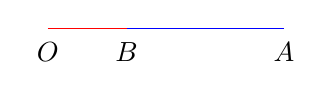
\begin{tikzpicture}
	\draw[blue] (0,0) -- (3,0);
	\draw[red] (0,0) -- (1,0);
	\draw (0,-0.3) node{$O$};
	\draw (3,-0.3) node{$A$};
	\draw (1,-0.3) node{$B$};
\end{tikzpicture}
\end{center}
	\item[$\alpha\beta$] Draw two lines $OA$ and $OB$ of length $|\alpha|$ and $|\beta|$ respectively (with a common end point $O$).
		Now draw the line of unit length $OP$ along the line $OB$.
		Construct triangle $OAP$.
		Draw the line $BQ$ parallel to the line $PA$ through $B$ such that $OQ$ and $OA$ are colinear.
		Now we have two similar triangles $OPA$ and $OBQ$.
		Then, the line $OQ$ of length $\| \alpha \beta \|$.
\begin{center}
\begin{tikzpicture}
	\draw[red] (0,0) -- (6,0);
	\draw (0,0) -- (3,0);
	\draw[blue] (0,0) -- (2.5,2);
	\draw (0,0) -- (1.25,1);
	\draw (2.5,2) -- (6,0);
	\draw (1.25,1) -- (3,0);
	\draw (0,-0.3) node{$O$};
	\draw (3,-0.3) node{$A$};
	\draw (1.25,1.3) node{$P$};
	\draw (2.5,2.3) node{$B$};
	\draw (6,-0.3) node{$Q$};
\end{tikzpicture}
\end{center}
	\item[$\alpha/\beta$] Draw two lines $OA$ and $OB$ of length $\| \alpha \|$ and $\| \beta \|$, with a common end point $O$.
		Draw a line of unit length $OP$ along the line $OB$.
		Now construct triangle $OBA$.
		Draw line $PQ$ parallel to $BA$ so that $OQ$ and $OA$ are colinear.
		Now the triangles $OAB$ and $OQP$ are similar.
		And the line $OQ$ has length $\| \alpha/\beta \|$.
\begin{center}
\begin{tikzpicture}
	\draw[red] (0,0) -- (6,0);
	\draw (0,0) -- (3,0);
	\draw[blue] (0,0) -- (1.5,2);
	\draw (0,0) -- (0.75,1);
	\draw (1.5,2) -- (6,0);
	\draw (0.75,1) -- (3,0);
	\draw (0,-0.3) node{$O$};
	\draw (3,-0.3) node{$Q$};
	\draw (0.60,1.06) node{$P$};
	\draw (1.5,2.3) node{$B$};
	\draw (6,-0.3) node{$A$};
\end{tikzpicture}
\end{center}
\end{description}
\end{proof}

\begin{corollary}
	The set of all constructible real numbers forms a subfield of the field of real numbers.
\end{corollary}
\begin{proof}
	The set of all constructible real numbers say $H$, contains both $0$ and $1$.
	since the line of length zero is trivial and line of unit length is provided.
	And we have, $\forall \alpha,\beta \in H,\ \alpha+\beta,\alpha-\beta,\alpha\beta,\alpha/\beta \in H$.
	Since $\alpha - \beta \in H$, $0-\beta = -\beta$ which is the additive inverse of $\beta$.
	And $1/\beta = \beta^{-1}$ is the multiplicative inverse of $\beta$.
	Thus, the set of all constructible numbers is a subfield of $\mathbb{R}$.
\end{proof}

\begin{theorem}
	The field of $F$ of constructible numbers consists {\color{blue}precisely} of all real numbers that we can obtain from $\mathbb{Q}$ by taking square root of positive numbers a finite number of times and applying a finite number of field operations.
\end{theorem}
\begin{proof}
	The constructible numbers are closed under field operations and forms a subfield $H$ of real numbers.
	We have, $\mathbb{Q}$ is the prime field of $\mathbb{R}$.
	That is, every subfield of $\mathbb{R}$ contains $\mathbb{Q}$.
	Thus, the subfield $H$ of constructible numbers contains $\mathbb{Q}$.
	That is, all the rational numbers are constructible.
	Therefore, it remains to prove that if $\alpha > 0$ is constructible then $\sqrt{\alpha}$ is also constructible.
\begin{center}
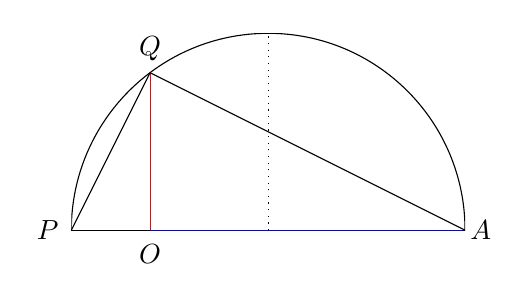
\begin{tikzpicture}
	\draw[blue] (0,0) -- (4,0);
	\draw (0,0) -- (-1,0);
	\draw[red] (0,0) -- (0,2);
	\draw (0,-0.3) node{$O$};
	\draw (4.2,0) node{$A$};
	\draw (-1.3,0) node{$P$};
	\draw (0,2.3) node{$Q$};
	\draw[dotted] (1.5,0) -- (1.5,2.5);
	\begin{scope}
		\clip (-1,0) rectangle (4,2.5);
		\draw (1.5,0) circle (2.5cm);
	\end{scope}
	\draw (4,0) -- (0,2);
	\draw (-1,0) -- (0,2);
\end{tikzpicture}
\end{center}

	Let $OA$ and $OP$ be colinear lines such that $OA$ be a line of length $\| \alpha \|$ and $OP$ be a line of unit length.
	Find the mid point of $PA$ and draw a circle of diameter $PA$.
	Then the length of the perpendicular $OQ$ from $PA$ to the circle is of length $\| \sqrt{\alpha} \|$ since $\Delta OAQ$ and $\Delta OQP$ are similar triangles.\\


	Therefore, real numbers obtained from rational numbers through finite number of additions/subtractions, multplications/divisions, and square root are constructible.
\end{proof}

\textbf{Note : } For example $\sqrt[4]{5\sqrt[8]{3}-2}$ is constructible, but $\sqrt[6]{2}$ and $\pi$ are not constructible.
We skip the proof that a real number which can't be obtained from rationals by a finite number of these operations is not constructible.
And assume that these three operations define the entire field of constructible numbers.

\begin{corollary}
	Let $\gamma$ be constructible number which is not rational.
	Then there exists a sequence of real numbers $\alpha_1,\alpha_2,\dots,\alpha_n = \gamma$ such that for every $i = 2,\dots,n$, the extension field $\mathbb{Q}(\alpha_1,\alpha_2,\dots,\alpha_i)$ is an extension of $\mathbb{Q}(\alpha_1,\alpha_2,\dots,\alpha_{i-1})$ of degree two.\\


	In other words, for any constructible number $\gamma$, $[\mathbb{Q}(\gamma) : \mathbb{Q}] = 2^n$ for some positive integer $n$.
\end{corollary}
\begin{proof}
	Let $\gamma$ be a constructible number which can be obtained from rationals by $n$ square root operations and a finite number of field operations.
	Then, we have a sequence of constructible numbers $\alpha_1, \alpha_2,\dots, \alpha_n$ such that $[\mathbb{Q}(\alpha_1,\alpha_2,\dots,\alpha_i) : \mathbb{Q}(\alpha_1,\alpha_2,\dots,\alpha_{i-1})] = 2$.
	Therefore, $[\mathbb{Q}(\gamma) : \mathbb{Q}] = 2^n$.
\end{proof}

	For example, $\gamma = \sqrt[4]{5\sqrt[8]{3}-2}$.
	Then $\alpha_1 = \sqrt{3}$, $\alpha_2 = \sqrt[4]{3}$, $\alpha_3= \sqrt[8]{3}$, $\alpha_4 = \sqrt{5\sqrt[8]{3}-2}$ and $\alpha_5 = \gamma$.
	Clearly, the geometric construction of $\gamma$ contains five instances of square root operation.

\subsection{Impossible Problems from Ancient Times}
\subsubsection{Doubling the cube}
\begin{theorem}
	There exists a cube such that it is impossible to construct the side of the cube with double the volume.
\end{theorem}
\begin{proof}
	Suppose the cube is of unit side.
	Then the side of the cube with double the volume is $\gamma = \sqrt[3]{2}$.
	And $irr(\gamma,\mathbb{Q}) = x^3-2$ and $[\mathbb{Q}(\sqrt[3]{2}:\mathbb{Q}] = 3 \ne 2^n$.
	Therefore, $\gamma$ is not constructible.
\end{proof}
\subsubsection{Squaring the circle}
\begin{theorem}
	There exists a circle such that it is impossible to construct the side of the square with the same area.
\end{theorem}
\begin{proof}
	Suppose the circle of is of unit radius.
	Then area of the circle is $2\pi$.
	And the side of the square with same area is $\sqrt{2\pi}$.
	Since $\pi$ is transcendental, $\pi$,$\sqrt{\pi}$ and $\sqrt{2\pi}$ are not constructible.
\end{proof}
\subsubsection{Trisecting an angle}
\begin{theorem}
	There exists an angle which can be trisected.
\end{theorem}
\begin{proof}
	We have $\cos 3\theta = 4\cos^3 \theta - 3\cos \theta$.
	Consider $\theta = 20^\circ$.
	Then $\gamma = \cos \theta$ is a root of the irreducible polynomial $4x^3-3x-0.5$.
	That is, $\gamma$ is a root of the monic irreducible polynomial $x^3-\frac{3}{4}x-\frac{1}{8}$ of degree $3$.
	Thus, $\gamma$ is not constructible, since $[\mathbb{Q}(\gamma) : \mathbb{Q}] = 3 \ne 2^n$.
\end{proof}
\subsection{Exercise \S32}
\begin{enumerate}
	\item
\end{enumerate}

\section{Finite Fields \S33}
\subsection{Structure of a Finite Field}
\begin{theorem}
	Let $E$ be a finite extension of degree $n$ over a finite field $F$.
	If $F$ has $q$ elements, then $E$ has $q^n$ elements.
\end{theorem}
\begin{proof}
	We have, extension field $E$ is an $n$-dimensional vector space over the field $F$.
	Let $\{ \alpha_1, \alpha_2,\dots, \alpha_n \}$ be a basis of the vector space $E$ over $F$.
	Then every elements of $E$ can be uniquely written as linear combination of basis vectors.
\begin{equation*}
 	\forall \beta \in E,\ \beta = b_1 \alpha_1 + b_2 \alpha_2 + \dots + b_n \alpha_n
\end{equation*}
	Suppose $\beta \in E$ has two distinct linear combinations.
	Then, the vectors $\{ \alpha_1, \alpha_2,\dots,\alpha_n\}$ are not linearly independent, which is a contraditciton.\\
	
	Since the representation is unique and $F$ has $q$ elements, there are $q^n$ distinct linear combinations possible.
	Therefore, $E$ has $q^n$ elements.
\end{proof}

\begin{corollary}
	If $E$ is a finite field of characteristic $p$.
	Then $F$ contains exactly $p^n$ elements for some integer $n$.
\end{corollary}
\begin{proof}
	We have, $E$ is a finite field of characteristic $p$.
	Thus, $\mathbb{Z}_p$ is the prime subfield of $E$.
	And $E$ is a finite extension of $\mathbb{Z}_p$.
	Thus, $E$ is a finite dimensional vector space over $\mathbb{Z}_p$.
	Let $n$ be the dimension of $E$ over $\mathbb{Z}_p$.
	And $\mathbb{Z}_p$ has $p$ elements.
	Therefore, $E$ has $p^n$ elements.
\end{proof}

\begin{theorem}
	Let $E$ be a field of $p^n$ elements contained in the algebraic closure $\overline{\mathbb{Z}_p}$ of $\mathbb{Z}_p$.
	Then the elements of $E$ are precisely the zeroes of the polynomial $x^{p^n}-x \in \mathbb{Z}_p[x]$.
\end{theorem}
\begin{proof}
	We have $E^\ast$ is a multiplicative group of non-zero elements in $E$.
	And $E^\ast$ has $p^n-1$ elements.
	Thus, order of any element $\alpha \in E^\ast$ should divide $p^n-1$.
	In other words, if $\alpha \in E^\ast$, then $\alpha^{p^n-1} = 1$.
	Clearly, $\alpha^{p^n} - \alpha = 0$, $\forall \alpha \in E$.
	However, $x^{p^n}$ can have atmost $p^n$ zeroes in $\overline{\mathbb{Z}_p}$.
	Thus, $E$ is precisely the set of all zeroes of $x^{p^n}-x \in \overline{\mathbb{Z}_p}$.
\end{proof}

%\begin{enumerate}[label=Note \arabic*]
%	\item The algebraic closure of $\mathbb{Z}_p$ contains zeroes of every polynomial of the form $x^{p^n}-x$ where $p$ is a prime and $n$ is an integer. Thus, algebraic closures are infinite fields. Remember : $\mathfrak{R}1$
%	\item $\overline{\mathbb{Z}_2}$ has two distinct square roots of unity. And the complex field contains only one of them !
%\end{enumerate}

\begin{description}
	\item[$n$th Root of Unity] $\alpha$ is an $n$th root of unity if $\alpha^n = 1$.
		ie, $\alpha = \sqrt[n]{1}$
	\item[Primitive $n$th Root of Unity] $\alpha$ is a primitive $n$th root of unity if $n$ is the smallest positive integer such that $\alpha^n = 1$.\\
		That is, $\alpha^n = 1$ and $\forall m \in \mathbb{N},\ m < n \implies \alpha^m \ne 1$
\end{description}

\begin{theorem}
	The multiplicative group of non-zero elements of a finite field $F$ is cyclic.
\end{theorem}
\begin{proof}
	Refer : \cite[Theorem 23.6]{fraleigh}
\end{proof}
\begin{corollary}
	Finite extension of finite fields are simple extensions.
\end{corollary}
\begin{proof}
	Let $E$ be a finite extension field of the finite field $F$.
	Then the multiplicative group of non-zero elements $E^\ast$ is cyclic.
	Let $\alpha$ be a generator of the cyclic group $E^\ast$.
	Then, $E = F(\alpha)$.
\end{proof}

\subsection{Galois Field $GF(p^n)$}
\begin{lemma}
	If $F$ is a field of prime characteristic $p$ with algebraic closure $\overline{F}$, then $x^{p^n}-x$ has $p^n$ distinct zeroes in $\overline{F}$.
\end{lemma}
\begin{proof}
	We have, $\overline{F}$ is algebraically closed.
	And $x^{p^n}-x \in \overline{F}[x]$.
	Thus, $x^{p^n}-x$ can be factorised into $p^n$ linear components.
	It remains to prove that these factors are distinct.\\

	Clearly, $0$ is a zero of multiplicity $1$, since $x^{p^n}-x = x (x^{p^n-1}-1)$.
	Let $\alpha \ne 0$ be a zero of $x^{p^n}-x$.
	Then $\alpha$ is a zero of $x^{p^n-1}-1$.
	ie, $\alpha^{p^n-1}  = 1$.
	\begin{align*}
		(x-\alpha)g(x) = & x^{p^n-1}-1 \\
		g(x) = & \frac{x^{p^n-1}-1}{x-\alpha}
		\intertext{By long division, we get}
		g(x) = & x^{p^n-2} + \alpha x^{p^n-3} + \alpha^2 x^{p^n-4} + \dots + \alpha^{p^n-3} x + \alpha^{p^n-2} \\
		g(\alpha) = & (p^n-1)\alpha^{p^n-2} \\
		= &(p^n-1)\frac{\alpha^{p^n-1}}{\alpha} \\
		= & p^n \frac{1}{\alpha} - \frac{1}{\alpha}\\
		= & -\frac{1}{\alpha} \ne 0
	\end{align*}
	Thus, every zero of $x^{p^n-1}-x$ is of multiplicity $1$.
\end{proof}

\begin{lemma}
	If $F$ is a field of prime characteristic $p$, then $(\alpha+\beta)^{p^n} = \alpha^{p^n} + \beta^{p^n}$.
\end{lemma}
\begin{proof}
	Since $F$ is a field of characteristic $p$, for every $\alpha \in F$, $p\alpha = 0$.
	\begin{align*}
		\intertext{ For $n=1$, we have }
		(\alpha+\beta)^p = & \alpha^p + p \alpha^{p-1}\beta+ \frac{p(p-1)}{2} \alpha^{p-2} \beta + \dots + p \alpha \beta^{p-1} + \beta^p \\
		= &  \alpha^p + 0 \alpha^{p-1}\beta+ 0 \alpha^{p-2} \beta + \dots + 0 \alpha \beta^{p-1} + \beta^p \\
		= & \alpha^p + \beta^p
	\end{align*}
	\begin{align*}
		\intertext{Suppose $(\alpha+\beta)^{p^{n-1}} = \alpha^{p^{n-1}} + \beta^{p^{n-1}}$, then} 
		(\alpha+\beta)^{p^n} = & \left[ (\alpha+\beta)^{p^{n-1}} \right]^p \\
		= & \left[ \alpha^{p^{n-1}} + \beta^{p^{n-1}} \right]^p \\
		= & \alpha^{p^n} + \beta^{p^n}
	\end{align*}
	Therefore, by mathematical induction the result is true.
\end{proof}

\begin{theorem}[Existence of Galois Field]
	For every prime power $p^n$, a finite field of $p^n$ elements exists.
\end{theorem}
{\color{blue} Hint : $\alpha^{p^n} = \alpha \iff \alpha^{p^n} - \alpha = 0 \iff \alpha$ is a zero of $x^{p^n} - x$}
\begin{proof}
	Consider the algebraic closure $\overline{\mathbb{Z}_p}$ of $\mathbb{Z}_p$.
	Let $K$ be a subset of $\overline{\mathbb{Z}_p}$ containing all zeroes of $x^{p^n}-x \in \overline{\mathbb{Z}_p}$.\\
	
	Let $\alpha, \beta \in K$.
	Then $\alpha^{p^n} = \alpha$ and $\beta^{p^n} = \beta$.
	Since $\overline{\mathbb{Z}_p}$ is a field of characteristic $p$, we have ${\color{blue}(\alpha+\beta)^{p^n} = \alpha^{p^n}+ \beta^{p^n}} = \alpha + \beta$.
	Thus, $(\alpha+\beta)$ is a zero of $x^{p^n}-x$.
	ie, $(\alpha + \beta) \in K$.
	Clearly, $(\alpha\beta)^{p^n} = \alpha^{p^n} \beta^{p^n} = \alpha\beta$.
	Thus, $\alpha\beta \in K$.\\


	Again $(-\alpha)^{p^n} = (-1 \cdot \alpha)^{p^n} = (-1)^{p^n} \cdot \alpha^{p^n} = -1 \cdot \alpha = -\alpha$.
	Thus, $-\alpha \in K$.
	Also $(\alpha^{-1})^{p^n} = \left( \frac{1}{\alpha} \right)^{p^n} = \frac{1}{\alpha^{p^n}} = \frac{1}{\alpha} = \alpha^{-1}$.
	Thus, $\alpha^{-1} \in K$.\\
	

	Trivially, $0,1 \in K$.
	Therefore, $K$ is a subfield of $\overline{\mathbb{Z}_p}$ with $p^n$ elements since {\color{blue}the $p^n$ zeroes of $x^{p^n}-x$ are distinct}.
\end{proof}

\begin{corollary}
	If $F$ is a finite field, then for every positive integer $n$, there exists an irreducible polynomial in $F[x]$ of degree $n$.
\end{corollary}
\begin{proof}
	Let $F$ be a finite field.
	Then $\mathbb{Z}_p$ is prime field of $F$ for some prime $p$.
	And $F$ is of characteristic $p$ and has $p^r$ elements for some positive integer $r$.\\ %The number of elements of $F$ should be multiple of prime $p$ and shouldn't be a multiple of any other prime $q$.


	Let $K$ be the subfield of $\overline{F}$ containing precisely all the zeroes of the polynomial $x^{p^{rn}}-x \in \mathbb{Z}_p[x]$.
	Then, $K$ has a subfield isomorphic to $\mathbb{Z}_p$ since $F$ is of characteristic $p$ and every subfield of $F$ has a subfield isomorphic to $\mathbb{Z}_p$.\\

	By existence theorem of Galois Fields, every element of $F$ is a zero of the polynomial $x^{p^r}-x \in \mathbb{Z}_p[x]$.
	That is, $\alpha \in F \iff \alpha^{p^r} = \alpha$.
	\begin{align*}
		\alpha^{p^{rn}} & = \left[\alpha^{p^r}\right]^{p^{r(n-1)}} & =  \alpha^{p^{r(n-1)}} & \\
		& = \left[\alpha^{p^r}\right]^{p^{r(n-2)}} & =  \alpha^{p^{r(n-2)}} & \\
		& \vdots & \vdots & \\
		& = \left[\alpha^{p^r}\right]^{p^r} & = \alpha^{p^r} & = \quad \alpha
	\end{align*}
	Thus, $\alpha \in F \implies \alpha^{p^{rn}} = \alpha \implies \alpha \in K$.
	Therefore $F$ is a subfield of $K$.
	Clearly, $K$ is a finite extension of the finite field $F$.
	And the vector space $K$ over $F$ is $n$-dimensional, since $K$ has $p^{rn} = [p^r]^n$ elements and $F$ has $p^r$ elements.\\
	
	Since every finite extension of finite fields are simple extensions, we have $K = F(\beta)$ and $irr(\beta,F) = n$.
	That is, there exists an unique monic, irreducible polynomial $p(x) \in F[x]$ of degree $n$ such that $p(\beta) = 0$.
	Therefore, $\forall n \in \mathbb{Z}^+$, there exists an irreducible polynomial in $F[x]$ of degree $n$.
\end{proof}


\begin{theorem}[Uniqueness of Galois Field]
	Let $p$ be a prime and $n$ a positive integer.
	If $E$ and $E'$ are fields of order $p^n$, then $E$ and $E'$ are isomorphic.\\

	There exists a unique finite field of order $p^n$, say \textbf{Galois Field}, $GF(p^n)$.
\end{theorem}
\begin{proof}
	Let $E,E'$ be fields of order $p^n$.
	Then both fields have $\mathbb{Z}_p$ as prime field.
	Thus, $E$ is a simple extension of $\mathbb{Z}_p$ of degree $n$.
	ie, $[E:\mathbb{Z}_p] = n$.
	And there exits an irreducible polynomial $f(x)$ such that $E \simeq \mathbb{Z}_p[x]/\generator{f(x)}$. \\


	Elements of $E$ are zeroes of $x^{p^n}-x$, thus $f(x)$ is a factor of $x^{p^n}-x$.
	Clearly, elements of $E'$ are zeroes of $x^{p^n}$ and therefore $E'$ has all zeroes of $f(x)$.
	And $E' \simeq \mathbb{Z}_p/\generator{f(x)}\simeq E$.
	Therefore, there exists a unique field of order $p^n$ (upto isomorphism), say $GF(p^n)$.
\end{proof}

\subsection{Exercise \S33}
\begin{enumerate}
	\item
\end{enumerate}

%Module 2
\section{Unique Factorisation Domains \S45}
\begin{definition}[divides]
	An element $a \in R$ divides $b$ if there exists an element $c \in R$ such that $b = ac$.
\end{definition}
\begin{definition}[associate]
	Two elements $a,b$ are associates if $a = bu$ where $u$ is a unit.
\end{definition}
\begin{definition}[UFD]
	\textbf{Unique factorisation domain}, UFD is an integral domain such that
	\begin{enumerate}
		\item Every element can be factored into a finite number of irreducibles, except 0 and units
		\dag\footnote{
			Unit is a element which has multiplicative inverse.}.
		\item The above factorisation is unique except for order and associates.
	\end{enumerate}
\end{definition}

For example, In $\mathbb{Z}$, $24 = 2 \times 2 \times 2 \times 3 = -2 \times -3 \times 2 \times 2$.
Here $2$ and $-2$ are associates.
And $2$ and $3$ are not units, since $2^{-1}, 3^{-1} \notin \mathbb{Z}$.

\begin{definition}[PID]
	An integral domain is $D$ is a \textbf{Principal Ideal Domain} if every ideal in $D$ is a principal ideal.
\end{definition}

%\subsection{Construction of UFD}
There are two important results on UFDs.
\begin{enumerate}
	\item Every PID is a UFD.
	\item If $D$ is a UFD, then $D[x]$ is a UFD.
\end{enumerate}

\subsection{Every PID is UFD}
%45.9
\begin{lemma}
	Let $R$ be a commutative ring and let $N_1 \subset N_2 \subset \dots $ be an ascending chain of ideals in $R$.
	Then $N = \cup_i N_i$ is an ideal of $R$.
\end{lemma}
\begin{proof}
	\textbf{Step 1 : $N$ is a subring of $R$}\\
	Suppose $N_i,\ N_j$ are two ideals in the chain, $N_i \subset N_j$ and $a \in N_i$, $b \in N_j$.
	Clearly, $a \in N_j$.\\

	And $a \pm b,\ ab \in N_j$.
	And $0 \in N_j \implies 0 \in N$.
	We have, $0$ in every ideal\dag\footnote{
		Suppose $b \in N$.
		We have $-b \in R$ and $-b+b = 0 \in bN \subset N$.}.
	Take $a = 0$, we know that for every element $b \in N_j$, its additive inverse $-b \in N_j$.
	Thus $b \in N \implies b \in N_j \implies -b \in N_j \implies -b \in N$.
	Clearly, $N$ is a subring of $R$.\\
	
	\textbf{Step 2 : $N$ is a ideal of $R$}\\
	Let $a \in N$ and $r \in R$.
	We have, $a \in N \implies a \in N_J$ for some ideal $N_j$ in the chain.
	Since $N_j$ is an ideal $ar = ra \in N_j$.
	Therefore, $ar \in N$.
	And $N$ is a ideal of $R$.
\end{proof}

\begin{lemma}[\textbf{A}scending \textbf{C}hain \textbf{C}ondition]
	Let $D$ be a PID.
	If $N_1 \subset N_2 \subset \dots$ is an ascending chain of ideal, then there exists a positive integer $r$ such that $N_r = N_s$ for every $s \ge r$.\\

	In other words, every strictly\dag\footnote{
		Strictly ascending chain : $N_1 \subsetneq N_2 \subsetneq N_3 \subsetneq \dots \subsetneq N_k$.}
	ascending chain of ideals in a PID is of finite length.
\end{lemma}
\begin{proof}
	Let $D$ be an integral domain.
	And $N_1 \subseteq N_2 \subseteq \dots$ be an ascending chain of ideals in $D$.
	Then $N = \cup_i N_i$ is an ideal in $D$.
	Since $D$ is a PID, by definition of \textbf{p}rincipal \textbf{i}deal \textbf{d}omain every ideal in it is a principal ideal.
	Thus, $N$ is a principal ideal in $D$.
	That is, there exists $c \in D$ such that $\generator{c} = N$.\\

	Since $c \in N$, and $N = \cup_i N_i$ we have $c \in N_r$ for some $r \in \mathbb{N}$.
	Then $\generator{c} = N_r = N$.
	Again, $N_r \subset N_s \implies c \in N_s \implies \generator{c} = N_s = N$.\\

	Suppose the chain of ideals are strictly ascending, that is every ideal in the chain is properly containing the former ideal.
	Then, the ideal $N_r$ such that $c \in N_r$ is the last ideal in its chain.
	Thus, striclty ascending chain of ideals is finite.
\end{proof}

\begin{theorem}
	Let $D$ be a PID.
	Every element that is neither $0$ nor a unit in $D$ is a product of irreducibles.
\end{theorem}
\begin{proof}
	Suppose $D$ is a PID.
	And suppose $a \in D$ is a neither a zero nor a unit.
	If $a$ is an irreducible, then the result is trivial.
	Suppose $a$ is not an irreducible.\\

	\textbf{Step 1 : $a$ has an irreducible factor}\\
	By the definition of irreducibility, $a$ has a factorisation $a = a_1b_1$ where $a_1,b_1$ are non-units.
	And every element $ar \in \generator{a}$ can be expressed as $ar = a_1b_1r = a_1r' \in \\generator{a_1}$.
	Thus, the ideal generated by $a$, $\generator{a}$ is contained in the ideal generated by $a_1$, $\generator{a_1}$.
	That is, $\generator{a} \subset \\generator{a_1}$.\\

	If $a_1$ is an irreducible, then the proof is complete.
	Suppose $a_1$ is not an irreducible.
	That is, $a_1 = a_2b_2$.
	Then $\generator{a_1} \subset \generator{a_2}$.
	Also we have, $\generator{a_1} \ne \generator{a_2}$.\\

	Suppose $\forall d \in D,\ a_2d \in \generator{a_1} \implies a_2\cdot 1 = a_2 \in \generator{a_1} \implies a_2 = a_1c_2 \implies a_1 = (a_1c_2)b_2 \implies c_2b_2 = 1 \implies b_2$ has multiplicative inverse $c_2$. This contradicts the assumption that $b_2$ is a unit.\\

	Continuing like this, we get a {\color{red}strictly} ascending chain of ideals $\generator{a} \subsetneq \generator{a_1} \subsetneq \generator{a_2}, \dots $.
	And we know that, every strictly ascending chain of ideals is finite.
	Thus, $a_r$ is an irreducible.
	And $a = a_1b_1 = (a_2b_2)b_1 = \dots = a_r(b_rb_{r-1}\dots b_1) = a_rb$.
	Clearly, $a$ has an irreducible factor $a_r$.\\

	\textbf{Step 2 : $a$ is a product of irreducibles}\\
	Suppose $a$ is neither zero nor a unit.
	Then $a = p_1c_1$ where $p_1$ is an irreducible and $c_1$ is not a unit.
	Continuing like this, we get another striclty ascending chain of ideals $\generator{a} \subsetneq \generator{c_1} \subsetneq \generator{c_2} \subsetneq \dots$ such that $a = p_1c_1 = p_1(p_2c_2) = \dots$ where $p_1,p_2,\dots$ are irreducibles and $c_j$ are non-units.
	Again, by ascending chain condition this strictly ascending chain is finite.
	That is, $a = p_1p_2\dots p_kc_k$ for some $k \in \mathbb{N}$.
	Since $\generator{c_k}$ is a maximal ideal in $D$, $c_k$ is an irreducible say, $p_{k+1}$.
	Thus, any element $a \in D$ (except zero and units) can be expressed as product of irreducibles.
\end{proof}

\subsection{Irreducible element and Maximal Ideal}
We have seen earlier that a non-trivial principal ideal $\generator{p(x)}$ in $F[x]$ is maximal if and only if the generator $p(x)$ is irreducible over $F$.
Now we have a generalisation, which says ideals in PIDs are maximal if and only if the generator is irreducible.
Remember that for any field $F$, $F[x]$ is a PID.
\begin{lemma}
	An ideal $\generator{p}$ in a PID is maximal if and only if $p$ is an irreducible.
\end{lemma}
\begin{proof}
	\textbf{Part A : $\generator{p}$ maximal in $D \implies p$ irreducible in $D$}\\
	Let $D$ be a PID.
	Suppose $\generator{p}$ is a maximal ideal in $D$.
	Suppose $p = ab$ in $D$.
	That is, $p = ab$ where $a,b \in D$.
	Then, $\generator{p} \subset \generator{a}$.\\

	Suppose $\generator{p} = \generator{a}$.
	Then $a = pc = (ab)c \implies bc = 1$ and $b$ is a unit.\\

	Suppose $\generator{p} \ne \generator{a}$.
	Then $\generator{a} = D$, since $\generator{p}$ is a maximal ideal.
	That is $\generator{a} = \generator{1} \implies a,1$ are associates.
	And $a$ is a unit.\\

	Thus for any factorisation $p = ab$, either $a$ or $b$ is a unit.
	Therefore, $p$ is an irreducible.\\

	\textbf{Part B : $p$ is irreducible in $D \implies \generator{p}$ is maximal in $D$}\\
	Suppose $p$ is an irreducible in $D$.
	Then $p = ab$ where $a,b \in D $ implies that either $a$ or $b$ is a unit.
	Since $p = ab$, $\generator{p} \subset \generator{a}$.
	We know that, if $a$ is a unit then $\generator{a} = \generator{1} = D$.\\

	Suppose $a$ is not a unit.
	Then $b$ is a unit.
	That is, there exists $u \in D$ such that $bu = 1$.
	Then $pu = abu= a$.
	Thus, $\generator{a} \subset \generator{p} \implies \generator{p} = \generator{a}$.\\

	Thus, for any factorisation $p = ab$, the ideals generated by $a,b$ are either $D$ or $\generator{p}$ itself.
	In other words, there doesn't exist a proper ideal containing $\generator{p}$.
	Therefore, $\generator{p}$ is a maximal ideal in $D$.
\end{proof}

\subsection{Every PID is UFD}
	We have seen earlier that $F[x]$ has unique factorisation of all its elements.
	Now, we generalise that result into ``every PID has unique factorisation for all its elements''.

\begin{lemma}
	In a PID, if an irreducible $p$ divides $ab$, then either $p|a$ or $p|b$.
\end{lemma}
\begin{proof}
	Let $D$ be a PID.
	Suppose $p \in D$ is irreducible.
	Suppose $p | ab$.
	Then $ab \in \generator{p}$.
	And we have, $\generator{p}$ is a maximal ideal.
	However, every maximal ideal in $D$ is a prime ideal.
	Thus, $ab \in \generator{p} \implies a \in \generator{p} \text{ or } b \in \generator{p}$.
	In other words, $p | a$ or $p | b$.
\end{proof}

\begin{corollary}
	If $p$ is an irreducible in a PID $D$ and $p$ divides $a_1a_2\dots a_n$ where $a_i \in D$, then $p|a_i$ for at least one $i$.
\end{corollary}
\begin{proof}
	We know that, $p | a_1a_2 \implies p | a_1 \text{ or } p | a_2$.\\
	Suppose $p | a_1a_2\dots a_k \implies p| a_1 \text{ or } p | a_2 \dots \text{ or } p | a_k$.\\
	Suppose $p | a_1a_2\dots a_{k+1} \implies p | a_1a_2\dots a_k \text{ or } p | a_{k+1}$.\\
	$\implies p|a_1 \text{ or } p|a_2 \text{ or } \dots p|a_k \text{ or } p | a_{k+1}$.\\
	That is, if $p$ divides a finite product, then it divides at least one of them.
\end{proof}

\begin{definition}
	A nonzero, nonunit element $p$ in an integral domain $D$ is a prime if $\forall a,b \in D,\ p|ab \implies p|a \text{ or } p|b$.
\end{definition}

\begin{theorem}
	Every PID is a UFD.
\end{theorem}
\begin{proof}
	Let $D$ be a PID.
	Let $a \in D$ is neither a zero nor a unit.
	Then $a$ has a factorisation into irreducibles $a= p_1p_2\dots p_r$. 
	Suppose $a$ has another factorisation $a = q_1q_2\dots q_s$.\\

	We have $p_1 | q_1q_2\dots q_s$.
	Thus, $p_1$ divides at least one of them, say $q_j$.
	Without loss of generality, we assume that $p_1 | q_1$ (rearranging the terms if necessary).\\

	Since $q_1$ is an irreducible, $q_1 = p_1u_1 \implies u_1$ is a unit.
	Thus, $p_1p_2 \dots p_r = p_1u_1q_2q_3\dots q_s$.
	That is, $p_2p_3 \dots p_r = u_1 q_2q_3\dots q_s$.\\

	Continuing like this we get, $p_r = u_1u_2\dots u_{r-1} p_ru_rq_{r+1}q_{r+s}\dots q_s$.
	Thus $u_1u_2\dots u_rq_{r+1}q_{r+2}\dots q_s$ is a unit.
	We have $s = r$, otherwise $1 = u_1u_2\dots q_{r+1}\dots$ is a contradiction.
	Therefore, any element $a \in D$ has a unique factorisation except for order,associates and units.
\end{proof}

\begin{corollary}
	The integral domain $\mathbb{Z}$ is a UFD.
\end{corollary}
\begin{proof}
	The ideals in $\mathbb{Z}$ are of the form $n\mathbb{Z}$ where $n \in \mathbb{Z}$.
	Thus every ideal in $\mathbb{Z}$ are pricipal ideals.
	Therefore, $\mathbb{Z}$ is a PID.
	We know that every PID is a UFD.
	Thus, $\mathbb{Z}$ is a \textbf{u}nique \textbf{f}actorisation \textbf{d}omain.
\end{proof}

\subsection{$D$ is UFD $\implies D[x]$ is UFD}
\begin{definition}[gcd]
	Let $D$ be a UFD and $a_1,a_2,\dots,a_n$ be nonzero elements in $D$.
	An element $d \in D$ is a \textbf{g}reatest \textbf{c}ommon \textbf{d}ivisor of $a_i$ if $d$ is a common divisor of all $a_i$s and also divides any common divisor of $a_i$s.
\end{definition}

\begin{definition}[primitive]
	Let $D$ be a UFD.
	A nonconstant polynomial $a_0 + a_1x + \dots + a_nx^n \in D[x]$ is a primitive if $1$ is the gcd of all $a_i$s.
\end{definition}
	For exmaple, $4x^3+3x^2+2 \in \mathbb{Z}[x]$ is a primitive since $\gcd(4,3,2) = 1$.

\begin{lemma}
	If $D$ is a UFD, then for every nonconstant $f(x) \in D[x]$ we have $f(x) = cg(x)$ where $c \in D$ and $g(x) \in D[x]$ and $g(x)$ is primitive.
	The element $c \in D$ is unique upto a unit factor in $D$ and is the \textbf{content} of $f(x)$.
	Also $g(x)$ is unique upto a unit factor in $D$.
\end{lemma}
\begin{proof}
	\textbf{Step 1 : There exists $c \in D$ such that $f(x) = cg(x)$}\\
	Let $f(x) = a_0 + a_1x + \dots +a_nx^n$ be a non-constant polynomial in $D[x]$.
	Let $c = gcd(a_0,a_1,\dots,a_n)$.
	In other words, $c$ is the greatest common divisor of the coefficients of $f(x)$.
	Let $q_i = ca_i)$.
	Clearly, $gcd(q_1,q_2,\dots,q_n) = 1$.
	Thus, we have $f(x) = cg(x)$ where $g(x) = q_0+q_1x+\dots+q_nx^n)$ is a primitive.\\

	\textbf{Step 2 : There exists unique $c$ such that  $f(x) = cg(x)$}\\
	Suppose $f(x) = cg(x) = dh(x)$ where $c,d \in D$ and $g(x), h(x)$ are primitives.\\

	Clearly, $c$ and $d$ are associates.
	Otherwise, there exists an irreducible element $p$ such that $p | cg(x)$ but $p\!\not|\ dh(x)$ which is a contradiction.
	Thus, we can cancel all irreducible factors of $c$ to obtain, $ug(x) = vh(x)$ where $u$ and $v$ are units.
	Therefore, the content of $f(x)$, $c$ unique upto associates.\\

	Again, $f(x) = cg(x) = (cu) (u^{-1}g(x))$ and thus $g(x)$ is unique upto associates/units.
\end{proof}

\begin{definition}[content]
	Let $D$ be a UFD.
	Let $f(x) \in D[x]$.
	Then $f(x) = cg(x)$ for some primitive $g(x) \in D[x]$ and $c \in D$.
	The element $c$ which is unique upto units, is the content of $f(x)$.
\end{definition}
	For example, Let $f(x) = 8x^3+6x^2+4 \in \mathbb{Z}[x]$.
	Then $f(x) = 2(4x^3+3x^2+2)$ where $4x^3+3x^2+2 \in \mathbb{Z}[x]$ is a primitive and $2 \in \mathbb{Z}$.
	Thus, $content(f) = 2$.

\begin{lemma}[Gauss]
	If $D$ is a UFD, then product of two primitive polynomials in $D[x]$ is again primitive.
\end{lemma}
\begin{proof}
	Let $f(x) = a_0 + a_1x + \dots + a_nx^n$ and $g(x) = b_0 + b_1x + \dots + b_mx^m$.
	Suppose $f(x)$ and $g(x)$ are primitives.
	Let $h(x) = f(x)g(x) = c_0 + c_1x + \dots + c_{n+m}x^{n+m}$.
	Let $p$ be an irreducible in $D$.
	Then $f(x)$ has a coefficient which is not divisible by $p$.
	Suppose $p$ divides every coefficient $f(x)$, then $f(x)$ is not a primitive.\\

	Let $r$ be the smallest integer such that $p\not\!|\ a_r$.
	Similarly, let $s$ be the smallest integer such that $p\not|\ b_s$.
	Now consider the coefficient $c_{r+s}$ of $h(x)$.
	$$ c_{r+s} = a_0b_{r+s}+\dots+a_{r-1}b_{s+1}+a_rb_s+a_{r+1}b_{s-1}+\dots+a_{r+s}b_0$$
	By the selection of $r$, $p | a_j$ for every $j < r$.
	Thus, $p | a_0b_s+\dots+a_{r-1}b_{s+1}$.
	Similarly, by the selection of $s$, $p | b_k$ for every $k < s$.
	Thus, $p | a_{r+1}b_{s-1}+\dots+a_0b_s$.
	Clearly, $p | c_{r+s} \iff p | a_rb_s \implies p|a_r \text{ or } p|b_s$.
	This is not possible, thus $p \not| c_{r+s}$.	
	Thus, for any irreducible $p \in D$, $h(x)$ has a coefficient which is not divisible by $p$.
	Therefore, product of two primitives is always a primitive.
\end{proof}

\begin{corollary}
	If $D$ is a UFD, then a finite product of primitive polynomials in $D[x]$ is again primitive.
\end{corollary}
\begin{proof}
	Let $\{f_k\}_{k=1}^n$ be a family of primitives.
	Then $f_1(x)f_2(x)$ is a primitive, since product of two primitives is always a primitive.\\

	Suppose $g(x) = f_1(x)f_2(x)\dots f_k(x)$ is a primitive.\\

	Consider $h(x) = f_1(x)f_2(x)\dots f_{k+1}(x) = g(x)f_{k+1}(x)$.
	Since both $g(x)$ and $f_{k+1}(x)$ are primitives their product $h(x)$ is also a primitive.\\

	Thus by finite mathematical induction, every finite product of primitives is a primitive.
\end{proof}

\begin{lemma}
	Let $D$ be a UFD and let $F$ be a field of quotients of $D$.
	Let $f(x) \in D[x]$ where $\deg f(x) > 0$.
	If $f(x)$ is an irreducible in $D[x]$, then $f(x)$ is also an irreducible in $F[x]$.
	Also, if $f(x)$ is primitive in $D[x]$ and irreducible in $F[x]$, then $f(x)$ is irreducible in $D[x]$.
\end{lemma}
\begin{proof}
	Let $D$ be a UFD and $F$ be the field of quotients of $D$.
	Then elements of $F$ are of the form $(a,b) \in D \times D$.
	Also $(a,b)+(c,d)  = (ad+bc,bd)$ and $(a,b)\cdot (c,d) = (ac,bd)$.
	And we say express $(a,b)$ as $a/b$.\\

	\textbf{Part 1 : irreducible in $D[x] \implies$ irreducible in $F[x]$}\\
	Let $f(x) \in D[x]$ be an irreducible in $D[x]$.
	Suppose $f(x)$ is not irreducible in $F[x]$.
	Then $f(x) = r(x)s(x)$ where $r(x),s(x) \in F[x]$.\\

	The coefficients of $r(x)$ are of the form $a/b$.
	By multiplying $r(x)$ with the product of all denominators, we can remove its denominators and obtain an associate $r_1(x) \in D[x]$.
	Similarly, we have $s(x) = vs_1(x)$ where $s_1(x) \in D[x]$.
	Thus, $f(x) = r(x)s(x) = ur_1(x)vs_1(x) = uv r_1(x)s_1(x)$.
	Therefore, $f(x) \in D[x]$ is not an irreducible, which is a contradiction.
	Thus, $f(x)$ is irreducible in the quotient field $F$ as well.\\

	\textbf{Part 2 : irreducible in $F[x] \implies$ irreducible in $D[x]$}\\
	Suppose $f(x) \in D[x]$ is irreducible in $F[x]$.	
	Clearly, $F$ contains a UFD isomorphic to $D$.
	Thus $D[x] \le F[x]$.
	Therefore, any polynomial irreducible in $F[x]$ is also irreducible in $D[x]$.
\end{proof}
	We just saw that if $F$ is the quotient field of a UFD $D$ and $f(x) \in D[x]$. The irreducibility of $f(x)$ in $F[x]$ is necessary and sufficient for the irreducibility of $f(x)$ in $D[x]$. Now we prove that the factorisation is also unique upto a morphism.

\begin{corollary}
	If $D$ is a UFD and $F$ is a field of quotients of $D$, then a nonconstant polynomial $f(x) \in D[x]$ factors into a product of two polynomials of lower degrees $r$ and $s$ in $F[x]$ if and only if it has a factorization into polynomials of the same degress $r$ and $s$.
\end{corollary}
\begin{proof}
	We know that if $f(x) \in D[x]$ has a factorisation $f(x) = r(x)s(x)$ in $F[x]$.
	Then it has a factorisation in $D[x]$ as well, $f(x) = cr_1(x)s_1(x)$ where $r_1(x),s_1(x)$ are associates of $r(x), s(x)$ in $F[x]$.
	Clearly, the associates are always of the same degree.\\

	Trivially, any factorisation in $D[x]$ will also be a factorisation in $F[x]$.
	And the factors will have the same degree, unless $D[x]$ has an irreducible polymonial which is not irreducible in $F[x]$.
	This is not possible.
\end{proof}

\begin{theorem}
	If $D$ is a UFD, then $D[x]$ is a UFD.
\end{theorem}
\begin{proof}
	Let $f(x) \in D[x]$.
	Suppose $deg(f) > 0$.
	Otherwise, $f(x)$ is a constant and we have trival factorisation.\\
	
	Let $f(x) = g_1(x)g_2(x)\dots g_r(x)$ be a factorisation in $D[x]$ with maximum number of factors.	
	Then $f(x) = c_1h_1(x)c_2h_2(x)\dots c_rh_r(x)$ where $g_k(x) = c_kh_k(x)$ and $h_k(x)$ are primitives.
	And $h_k(x)$ are irreducibles.
	Otherwise, $f(x)$ has a factorisation with greater number of factors than $r$ which is a contradiction.
	Thus, $f(x) = uh_1(x)h_2(x)\dots h_r(x)$ is a factorisation of $f(x)$ into a product of irreducibles.\\

	Suppose $f(x)$ has another factorisation $f(x) = G_1(x)G_2(x)\dots G_r(x)$.
	Then $f(x) = vH_1(x)H_2(x)\dots H_r(x)$ with $H_k(x)$ are all irreducibles.
	We know that, $h_k(x) | f(x) \implies h_k(x) | H_1(x)H_2(x)\dots H_r(x) \implies h_k(x) | H_k(x)$ (WLOG).
	Therefore, the factorisation is unique.
\end{proof}

For example, let $x,y$ be two indeterminates, then an element $f(x) \in F[x,y]$ is of the form $\displaystyle\sum_{i,j = 0}^{n,m} a_{ij}x^i y^j$.

\begin{corollary}
	If $F$ is a field of quotients and $x_1,x_2,\dots,x_n$ are indeterminates, then $F[x_1,x_2,\dots,x_n]$ is a UFD.
\end{corollary}
\begin{proof}
	Suppose $D$ is a UFD and $F$ is its field of quotients, then $F[x]$ is a UFD.\\

	Suppose $K = F[x_1,x_2,\dots,x_k]$ is a UFD.\\

	Then, $F[x_1,x_2,\dots,x_k,x_{k+1}] = F[x_1,x_2,\dots,x_k][x_{k+1}] = K[x_{k+1}] = K[x]$ is a UFD.
\end{proof}

\subsection{Exercise \S45}
\begin{enumerate}
	\item
\end{enumerate}

\section{Euclidean Domain \S46}
\begin{definition}[Euclidean Norm]
	Euclidean norm on an integral domain $D$ is a function $v$ which maps non-zero elements of $D$ into non-negative integers such that 
	\begin{enumerate}
		\item $\forall a,b \in D, (b \ne 0)$ there exists $q,r \in D$ such that $a = qb + r$ where  either $r = 0$ or $v(r) < v(b)$ and 
		\item $\forall a,b \in D, (a,b \ne 0)$ $v(a) \le v(ab)$
	\end{enumerate}
\end{definition}
\begin{definition}[Euclidean Domain]
	An integral domain $D$ is a Euclidean Domain if there exists a Euclidean Norm in $D$.
\end{definition}
For example, $v(n) = |n|$ is a Euclidean norm on Euclidean domain $\mathbb{Z}$. And $v(f(x)) = deg(f(x))$ is a Euclidean norm on Euclidean domain $F[x]$.

\begin{theorem}
	Every Euclidean domain is a PID.
\end{theorem}
\begin{proof}
	Let $D$ be a Euclidean domain with Euclidean norm $v$.
	Let $N$ be an ideal in $D$.
	If $N = \{ 0\}$, then $N = \generator{0}$ is a principal ideal.\\

	Suppose $N \ne \{ 0 \}$.
	Then there exists $b \in N\ (b \ne 0)$.
	Clearly, $b \in N \implies \generator{b}\subset N$.
	Choose a $b \in N$ such that $v(b)$ is minimal in $N$.\\

	\textbf{Claim : $N = \generator{b}$}\\
	Let $a \in N$.
	Then there exists $q,r \in D$ such that $a = qb + r$ where $r = 0$ or $v(r) < v(b)$.
	Clearly, $r = a-qb \in N$.
	Thus, $r = 0$ since $v(r) < v(b)$ and $v(b)$ is minimal in $N$.
	That is, $a = qb$ or $b|a$ for every $a \in N$.
	Thus, $N \subset \generator{b}$.
	Therefore, $N = \generator{b}$.
	In other words, evey ideal in $D$ is a principal ideal.
\end{proof}

\begin{corollary}
	Every Euclidean domain is a UFD.
\end{corollary}
\begin{proof}
	We know that, every Euclidean domain is a PID.
	And every PID is a UFD.
	Thus, every Euclidean domain is a UFD.
\end{proof}
\subsection{Arithmetic in Euclidean Domain}
\begin{theorem}
	For a Euclidean domain with Euclidean norm $v$, $v(1)$ is minimal and $u \in D$ is a unit if and only if $v(u) = v(1)$.
\end{theorem}
\begin{proof}
	We have, $v(a) \le v(ab)$.
	Take $a = 1$, $v(1) \le v(1b) \implies v(1) \le v(b)$ for every $b \in D$.
	Thus, $v(1)$ is minimal.\\

	Suppose $u$ is a unit with multplicative inverse $u^{-1}$.
	Clearly, $v(1) \le v(u)$ since $u \in D$.
	Take $a = u$ and $b = u^{-1}$.
	Then $v(u) \le v(uu^{-1}) = v(1)$.
	Therefore, for every unit $u \in D$, we have $v(u) = v(1)$.
\end{proof}

\begin{theorem}[division algorithm]
	Let $D$ be a Euclidean domain with Euclidean norm $v$.
	And $a,b \in D\ (a,b \ne 0)$.
	\begin{align*}
		a = & bq_1 + r_1, \text{ where } r_1 = 0 \text{ or } v(r_1) < v(b)
		\intertext{if $r_1 \ne 0$}
		b = & r_1q + r_2, \text{ where } r_2 = 0 \text{ or } v(r_2) < v(r_1)
		\intertext{ In general, if $r_i \ne 0$}
		r_{i-1} = & r_iq + r_{i+1} \text{ where } r_{i+1} = 0 \text{ or } v(r_{i+1}) < v(r_i)
	\end{align*}
	Then the sequence $r_1,r_2, \dots$ must terminate with some $r_s = 0$.\\

	If $r_1 = 0$, then $gcd(a,b) = b$.\\
	If $r_k = 0$, then $gcd(a,b) = r_{k-1}$.\\

	Furthermore, if $d$ is a gcd of $a$ and $b$, then there exists $\lambda,\mu \in D$ such that $d= \lambda a + \mu b$.
\end{theorem}
\begin{proof}
	\textbf{Step 1 : Finite Sequence  $r_1,r_2,\dots,r_s$}\\
	Suppose $r_1,r_2,\dots,r_{i-1} \ne 0$.
	Then $v(r_1) > v(r_2) > \dots > v(r_{i-1})$ is a strictly decreasing sequence of non-negative integers.
	Thus, the sequence will terminate in finite numbers of steps.
	That is, $r_s = 0 $ for some integer $s$.\\
	
	\textbf{Step 2 : $gcd(a,b) = r_{s-1}$}\\
	Suppose $r_1 = 0$.
	Then $a = bq$ and $gcd(a,b) = b$ since $b|a, b|b$ and there does not exist an integer greater than $b$ that divides $b$.\\

	Suppose $r_1 \ne 0$ and $gcd(a,b) = d$.
	Then $r_1 = a-bq$ and $d|r_1$.\\
	And $d | b, d | r_1 \implies d|a$ since $a = qb+r_1$.
	Thus, $gcd(a,b) = gcd(b,r_1)$.\\
	Continuing like this, we get $gcd(a,b) = gcd(r_{s-2},r_{s-1})$ if $r_{s-1} \ne 0$.\\
	And we have, $r_s = 0 \implies r_{s-2} = qr_{s-1}$.\\
	Clearly, $gcd(r_{s-2},r_{s-1}) = r_{s-1} = gcd(a,b)$.\\

	\textbf{Step 3 : $gcd(a,b) = \lambda a + \mu b$}\\
	Let $b$ be a $gcd(a,b)$.
	Then, $b = 0a+1b$ and result is complete.\\

	Suppose $gcd(a,b) = r_{s-1}$.
	And $r_{s-1} = r_{s-3} - qr_{s-2}$.
	Clearly, $r_i = \lambda_i r_{i-2} + \mu_i r_{i-1}$.
	Keep on substituting using these equations until we reach $r_{s-1} = \lambda a + \mu b$.\\

	Suppose $d'$ is another $gcd(a,b)$.
	Then $d' = ud$ is an associate of $d$.
	And $d' = ud = (\lambda u)a + (\mu u) b$.
	And the result is true for any $gcd(a,b)$.
\end{proof}

\section{Gaussian Integers and Multiplicative Norms \S47}
\subsection{Gaussian Integers and Norm}
\begin{definition}[Gaussian integers]
	Gaussian integers are complex numbers of the form $a+ib$ where $a,b \in \mathbb{Z}$.
\end{definition}
Note : Let $\alpha = a+ib$.
Clearly, Gaussian integers are elements of $\mathbb{Z}[i]$.
Here, $\mathbb{Z}[i]$ is a simple extension of the integral domain $\mathbb{Z}$ with a zero of $x^2+1$.

\begin{definition}[Gaussian Norm]
	Let $\alpha = a+ib$ be a Gaussian integer.
	Then $N(\alpha) = |\alpha|^2 = a^2+b^2$ is a Euclidean norm on $\mathbb{Z}[i]$.
\end{definition}

\begin{lemma}
	The Gaussian norm $N : \mathbb{Z}[i] \to \mathbb{Z}$ defined by $N(a+ib) = a^2+b^2$ has the following properties
	\begin{enumerate}
		\item $N(\alpha) \ge 0,\ \forall \alpha \in \mathbb{Z}[i]$
		\item $N(\alpha) = 0 \iff \alpha = 0$
		\item $N(\alpha\beta) = N(\alpha)N(\beta)$
	\end{enumerate}
\end{lemma}
\begin{proof}
	We have $\alpha \in \mathbb{Z}[i]$.
	Then $\alpha = a+ib$ where $a,b \in \mathbb{Z}$.
	Clearly, $N(a+ib) = a^2+b^2 \ge 0$.\\

	$N(\alpha) = 0 \iff a^2+b^2 = 0 \iff a=0,b=0 \iff \alpha = 0+i0 = 0$.\\

	Also, $N(\alpha\beta) = |\alpha\beta|^2 = |\alpha|^2 |\beta|^2 = N(\alpha)N(\beta)$.
\end{proof}

\begin{lemma}
	$\mathbb{Z}[i]$ is an integral domain.
\end{lemma}
\begin{proof}
	Let $\alpha, \beta \in \mathbb{Z}[i]$.\\
	Then, $\alpha + \beta = (a+ib) + (c+id) = (a+c) + i(b+d) = (c+a) + i(d+b) = \beta + \alpha$.
	And for any $\alpha \in \mathbb{Z}[i]$, we have $\alpha \cdot 1 = (a+ib) \cdot (1+i0) = (a+ib)$.
	Thus, we have $\mathbb{Z}[i]$ is a commutative ring with unity.\\

	It remains to prove that $\mathbb{Z}[i]$ has no zero divisors.
	Suppose $\alpha\beta = 0$.
	$\alpha\beta = 0 \implies N(\alpha\beta) = 0 \implies N(\alpha) N(\beta) = 0$.
	But, $N(\alpha),N(\beta) \in \mathbb{Z}$ and $\mathbb{Z}$ has no zero divisors.
	Thus, $N(\alpha) = 0$ or $N(\beta) = 0 \implies \alpha = 0$ or $\beta = 0$.
	Therefore $\mathbb{Z}[i]$ has no zero divisors.
\end{proof}

\begin{theorem}[Gaussian integers is a Euclidean Domain]
	The function $v$ defined by $v(\alpha) = N(\alpha)$ for every non-zero $\alpha \in \mathbb{Z}[i]$ is a Euclidean norm.
\end{theorem}
\begin{proof}
	\textbf{Step 1 : $v(a) \le v(ab)$}\\
	Let $\beta = b_1 + ib_2$ and $\beta \ne 0$.
	Then $N(\beta) = b_1^2+b_2^2 \ge 1$.
	Thus, $N(\alpha) \le N(\alpha)N(\beta) = N(\alpha\beta)$.\\

	\textbf{Step 2 : Division algorithm}\\
	That is, $\forall \alpha,\beta \in \mathbb{Z}[i],(\beta \ne 0)\ \exists \sigma,\rho \in \mathbb{Z}[i]$ such that $\alpha = \beta\sigma+\rho$, and $\rho = 0$ or $v(\rho) < v(\beta)$.

	Since $\beta \ne 0$, $\alpha/\beta$ exists.
	And we have, $\frac{\alpha}{\beta} = \frac{a_1+ia_2}{b_1+ib_2} = \frac{(a_1+ia_2)(b_1-ib_2)}{(b_1+ib_2)(b_1-ib_2)} = \frac{a_1b_1+a_2b_2}{b_1^2+b_2^2} + i \frac{a_2b_1-a_1b_2}{b_1^2+b_2^2} = r+is$ where $r,s \in \mathbb{Q}$.
	Consider integers $q_1,q_2$ that are nearest to the rational numbers $r,s$.
	Define $\sigma = q_1 + iq_2 \in \mathbb{Z}[i]$ and $\rho = \alpha - \beta\sigma$.\\

	Suppose $\rho \ne 0$.
	If $\rho = 0$, then the proof is complete.
	By definition of $\sigma$, $|q_1-r| \le 0.5$ and $|q_2-s| \le 0.5$.
	And we have, $$N \left(\frac{\alpha}{\beta} - \sigma \right) = N((r-q_1)+i(s-q_2)) = |q_1-r|^2 + |q_2-s|^2 \le 0.5$$
	Since $\alpha = \beta\sigma + \rho$,
	we have $\rho = \beta(\frac{\alpha}{\beta}-\sigma)$
	$$N(\rho) = N \left( \beta \left(\frac{\alpha}{\beta}-\sigma \right) \right) = N(\beta) N \left(\frac{\alpha}{\beta}-\sigma\right) \le 0.5N(\beta)$$
	Thus, $N(\rho) < N(\beta)$.
	Therefore, Gaussian integers is a Euclidean domain.
\end{proof}

\subsection{Multiplicative Norm}
\begin{definition}[multiplicative norm]
	Let $D$ be an integral domain. A function $N : D \to \mathbb{Z}$ is a multiplicative norm if 
	\begin{enumerate}
		\item $N(\alpha) = 0 \iff \alpha = 0$
		\item $N(\alpha\beta) = N(\alpha)N(\beta),\ \forall \alpha,\beta \in D$
	\end{enumerate}
\end{definition}
Note : Guassian norm is a multiplicative norm.

\begin{theorem}
	Let $D$ be an integral domain with multiplicative norm $N$.
	Then $N(1) = 1$ and $|N(u)| = 1$ for any unit $u$.
	Suppose $|N(\alpha)| = 1$ only for units  in $D$.
	Then $N(\alpha)$ is a prime in $\mathbb{Z}$ implies $\alpha$ is an irreducible in $D$.
\end{theorem}
\begin{proof}
	We know, $N$ is a multiplicative norm.
	Thus, $N(1) = N(1 \ast 1) = N(1)N(1) \implies N(1) = 1$.\\

	Suppose $u$ is a unit in $D$.
	Then $1 = N(1) = N(uu^{-1}) = N(u) N(u^{-1})$
	Since $1$ has only two factors $\pm 1 \in \mathbb{Z}$, we have $|N(u)| = 1$.\\

	Suppose $|N(\alpha)| = 1$ only if $\alpha$ is a unit in $D$.
	Suppose $\alpha \in D$ and $|N(\alpha)| = p$, where $p$ is a prime in $\mathbb{Z}$.
	Suppose $\alpha$ is not an irreductible.
	Then $\alpha$ has a factorisation $\alpha = \beta\gamma$ where $\beta,\gamma \in D$ are non-units.
	Then $p = N(\alpha) = N(\beta\gamma) = N(\beta)N(\gamma)$.
	We have, $\beta,\gamma$ are non-units and $|N(\beta)| \ne 1$ and $|N(\gamma)| \ne 1$.
	This is not possible.
	Therefore, $\alpha$ is an irreducible in $D$.
\end{proof}

\subsection{Applications of multiplicative norm}
\subsubsection{The integral domain $\mathbb{Z}[\sqrt{-5}]$ is not a UFD.(\S47.9)}
\begin{proof}
Elements of $\mathbb{Z}[\sqrt{-5}]$ are of the form $a+b\sqrt{-5}$ and $N(a+b\sqrt{-5}) = a^2 + 5b^2$.
If $N(a+b\sqrt{-5}) = a^2+5b^2 = 1$, then, $a = \pm 1$ and $b = 0$.
Clearly, $|N(\alpha)| = 1$ only if $\alpha$ is a unit in $\mathbb{Z}[\sqrt{-5}]$.\\

The element $3 \in \mathbb{Z}[\sqrt{-5}]$ is an irreducible.
Suppose $3$ is not an irreducible.
That is, there is a factorisation $3 = \beta\gamma$ where $\beta,\gamma$ are non-units.
Then $9 = N(3) = N(\beta)N(\gamma)$ where $\beta,\gamma$ are non-units.
The integer factors of $9$ are $1,3,9$.
Thus, $N(\beta) = N(\gamma) = 3$.
Otherwise $N(\beta) = 1$ or $N(\gamma) = 1$.
But, there doesn't exist an element $a+b\sqrt{-5}$ such that $N(a+b\sqrt{-5}) = 3$.
Similarly, $7 \in \mathbb{Z}[\sqrt{-5}]$ is an irreducible.
We have, $49 = N(7) = N(\beta)N(\gamma) \implies N(\beta)=N(\gamma) = 7$ is not possible since there are no elements of norm $7$ in $\mathbb{Z}[\sqrt{-5}]$.\\

Suppose $(1+2\sqrt{-5})$ is not an irreducible.
Then, $21 = N(1+2\sqrt{-5}) = N(\beta)N(\gamma)$.
However, we know that the integer factors of $21$ are $1,3,7,21$.
Without loss of generality, we have $N(\beta) = 3$ which is not possible.
Thus, $1+2\sqrt{-5}$ is an irreducible.\\

However neither $3$ nor $7$ is an associate of $1+2\sqrt{-5}$.
Since $|N(1+2\sqrt{-5})| \ne N(3)$ and $N(1+2\sqrt{-5}) \ne N(7)$.
Clearly, the factorisation of $21 \in \mathbb{Z}[\sqrt{-5}]$ is not unique.
Therefore, $\mathbb{Z}[\sqrt{-5}]$ is not a UFD.
\end{proof}
\subsubsection{Fermat's $p = a^2+b^2$ theorem}
\begin{theorem}[Fermat]
	Let $p$ be an odd prime integer.
	Then $p = a^2 + b^2$ where $a,b \in \mathbb{Z}$ if and only if $p \cong 1 \pmod{4}$
\end{theorem}
\begin{proof}
	Suppose there exists an odd prime $p$ such that $p = a^2 + b^2$.
	Then $a,b$ are of different parity.
	Without loss of generality, $a$ is even and $b$ is odd.
	Let $a=2r$ and $b=2s+1$.
	Then $a^2+b^2 = 4r^2 + 4s^2 + 1 \cong 1 \pmod{4}$.\\

	Suppose $p \cong 1 \pmod{4}$.
	Then $\mathbb{Z}_p$ is a cyclic group of order $p-1$ which has a element $n$ of order $4$ since $4|(p-1)$.
	Then $n^2 = -1 \in \mathbb{Z}_p$.
	And $n^2+1 \cong 0 \pmod{p}$.
	In other words, $p | (n^2+1)$.\\

	We claim that, $p$ is not an irreducible in $\mathbb{Z}[i]$.
	Suppose $p$ is an irreducible then $p|(n^2+1) \implies p|(n+i)$ or $p|(n-i)$.
	And $p|(n+i) \implies n+i = p(a+bi) \implies n= pa \text{ and }1 = pb$.
	But, $1=pb$ is not possible.
	Similarly, $p|(n-i) \implies n-i = p(a+bi) \implies -1 = pb$ is also not possible.
	Thus if $p \cong 1 \pmod{4}$, then $p$ is not an irreducible in $\mathbb{Z}[i]$.\\

	Since $p$ is not an irreducible in $\mathbb{Z}[i]$.
	$p = (a+bi)(c+di)$ where $a+bi,c+di$ are non-units in $\mathbb{Z}[i]$.
	Considering the Gaussian norm $N$ on $\mathbb{Z}[i]$ defined by $N(a+bi) = a^2 + b^2$.
	We have, $p^2 = N(p) = N(a+bi)N(c+di) = (a^2+b^2)(c^2+d^2)$.
	And $N((a+bi) \ne 1$ since for Gaussian norm $N(\alpha) = 1 \iff \alpha = 1$.
	Similarly, $N(c+di) \ne 1$.
	Therefore, without loss of generality $N(a+bi) = p$ since $a^2+b^2 > 0$.
	In other words, $p = a^2 + b^2$.
\end{proof}
\subsection{Exercise \S47}
\begin{enumerate}
	\item We have $5$ is an odd prime and  $5 \cong 1 \mod{4}$.
		Therefore $5$ is not an irreducible Gaussian integer.
		Clearly, $2^2+1^2 = 5 \implies (2+i)(2-i) = 5$.\\

		And $N(2+i) = 5$ is a prime, thus $2+i$ is an irreducible.
		Similarly, $2-i$ is also an irreducible.
		Therefore $5 = (2+i)(2-i)$ is factorisation using irreducibles Gaussian integers.
		(hint : $2^2+1^ = 5$. But, $1 \ast 1 + 2 \ast 2 = 5$)\\

		Note : We have $ 5 = (2+i)(2-i) = (1+2i)(1-2i)$.
		However $5$ has a unique factorisation since $(2+i)$ and $(1-2i)$ are associates $(2+i)(0-i) = 1-2i$ where $-i \in \mathbb{Z}[i]$ is a unit with multiplicative inverse $i$.

	\item We have $7$ is an odd prime.
		However $7 \cong 3 \pmod{4}$.
		Therefore $7$ is an irreducible Gaussian integer.
	\item We have $N(4+3i) = 25$.
		Clearly, $(4+3i) = \alpha\beta \implies N(\alpha) = N(\beta) = 5$.
		Therefore, $4+3i = (2-i)(1+2i)$ is a factorisation of $4+3i$.
		(Hint : $2^2+1^2 = 5$. But, $1 \ast 2 + 1 \ast 2 = 4$.)
	\item We have $N(6-7i) = 85 = 5 \ast 17$.
		Clearly $6-7i = (2+i)(1-4i)$.
		(Hint : $2^2+1^2 = 5$ and $4^2+1^2 = 17$. But $1 \ast 2 + 1 \ast 4 = 6$.)
	\item We have $6 = 2 \ast 3$ in $\mathbb{Z}[\sqrt{-5}]$.
		Then, $N(\alpha\beta) = 4 \implies a^2+5b^2 = 2$ is not possible.
		And, $N(\alpha\beta)= 9 \implies a^2+5b^2 = 3$ is also not possible. Therefore, $6 = 2 \ast 3$ is a factoriation in $\mathbb{Z}[\sqrt{-5}]$.\\

		However $N(\alpha\beta) = 6 \implies a^2 + 5b^2 = 6 \implies |a| = |b| = 1$.
		Clearly, $6 = (1-\sqrt{-5})(1+\sqrt{-5})$ is another factorisation.
\end{enumerate}
%Module 3
\section{Automorphism and Fields \S48}
\section{The Isomorphism Extension Theorem \S49}
\section{Splitting Fields \S50}

%Module 4
\section{Separable Extensions \S51}
\section{Galois Theory \S53}
\section{Illustrations of Galois Theory \S54}
\section{Cyclotomic Extensions \S55}

\chapter{ME010202 Advanced Topology}
%Text Books : \cite{joshi}, \cite{munkres}
%Module 1: Separation axioms
%Compactness and Separation axioms , The Urysohn Characterisation of normality, Tietze Characterisation of normality.
%( Chapter 7: Sections 2; 2.1 to 2.10 Section 3; 3.1 to 3.6 – Proof of Lemma 3.4 excluded Section 4; 4.1 to 4.7 of \cite{joshi}) (20hours)
%Module 2: 
%Products and Co-products - Cartesian products of families of sets – The product topology -Productive properties.
%( Chapter 8 : Section 1; 1.1 to 1.9 Section 2; 2.1 to 2.8 , Section 3 – 3.1 to 3.6 of \cite{joshi}) (25hours)
%Module 3: 
%Embedding and Metrisation - Evaluation functions into products, Embedding lemma and Tychonoff Embedding, The Urysohn Metrisation Theorem.
%Variation of compactness
%( Chapter 9: Section 1; 1.1 1.5, Section 2; 2.1 to 2.5 Section, 3; 3.1 to 3.4 of \cite{joshi})
%(Chapter 11: Sections 1.1 to 1.11 of \cite{joshi}) (25 hours)
%Module 4:
%Definition and convergence of nets, Homotopy of paths.
%(Chapter 10: Section 1 of \cite{joshi})
%(Chapter 9 : Section 1 of \cite{munkres}) (20hours)

%Need to plan this topic with activities

%Module 1 - \cite{joshi} 7
%Module 2 - \cite{joshi} 8
%Module 3 - \cite{joshi} 9
%Module 4 - \cite{joshi} 10, \cite{munkres} 9

%Warning : The results are reordered for presentation
%Obviously, forward references will occur.

%\chapter{Separation Axioms}
\section{Module I}
\begin{commentary}
	\textbf{Q : } Why these axioms are called separation axioms ?\\
	$T_0,T_1,T_2$ axioms separates points from points.\\
	$T_3,T_{3\frac{1}{2}}$ axioms separates points from closed subsets.\\
	$T_4$ axiom separates closed subsets from closed subsets.
\end{commentary}
\begin{figure}[h]
	\centering
	\begin{tikzpicture}[line cap=round,line join=round,>=triangle 45,x=1.0cm,y=1.0cm, scale=0.5]
%	\clip(-4.3,-5.46) rectangle (12.4,6.3);
	\draw (2.3,1.62) circle (1.99cm);
	\draw (2.1,1.36) circle (1.02cm);
	\begin{scriptsize}
	\draw (2.58,4.1) node {X};
	\fill (2.1,1.36) circle (1.5pt);
	\draw (2.24,1.12) node {x};
	\draw (2.3,2.62) node {U};
	\fill (3.64,1.54) circle (1.5pt);
	\draw (3.78,1.2) node {y};
	\draw (2.5,-1) node {$T_0$};
	\end{scriptsize}
	\end{tikzpicture}
	\begin{tikzpicture}[line cap=round,line join=round,>=triangle 45,x=1.0cm,y=1.0cm,scale=0.5]
%	\clip(-4.3,-5.46) rectangle (12.4,6.3);
	\draw (2.3,1.62) circle (1.99cm);
	\draw (2.1,1.36) circle (1.28cm);
	\draw (3.64,1.54) circle (0.55cm);
	\begin{scriptsize}
	\draw (2.58,4.1) node {X};
	\fill (2.1,1.36) circle (1.5pt);
	\draw (2.28,1.06) node {x};
	\draw (2.16,2.94) node {U};
	\fill (3.64,1.54) circle (1.5pt);
	\draw (3.82,1.28) node {y};
	\draw (3.74,2.32) node {V};
	\draw (2.5,-1) node {$T_1$};
	\end{scriptsize}
	\end{tikzpicture}
	\begin{tikzpicture}[line cap=round,line join=round,>=triangle 45,x=1.0cm,y=1.0cm,scale=0.5]
%	\clip(-4.3,-5.46) rectangle (12.4,6.3);
	\draw (2.64,1.46) circle (1.99cm);
	\draw (2.1,1.36) circle (0.78cm);
	\draw (3.64,1.54) circle (0.59cm);
	\begin{scriptsize}
	\draw (2.92,3.94) node {X};
	\fill (2.1,1.36) circle (1.5pt);
	\draw (2.28,1.06) node {x};
	\draw (2.42,2.52) node {U};
	\fill (3.64,1.54) circle (1.5pt);
	\draw (3.82,1.18) node {y};
	\draw (3.72,2.36) node {V};
	\draw (3,-1) node {$T_2$};
	\end{scriptsize}
	\end{tikzpicture}
	\begin{tikzpicture}[line cap=round,line join=round,>=triangle 45,x=1.0cm,y=1.0cm,scale=0.5]
%	\clip(-4.3,-5.46) rectangle (12.4,6.3);
	\draw (2.64,1.46) circle (1.99cm);
	\draw (2.1,1.36) circle (0.83cm);
	\draw (3.64,1.54) circle (0.59cm);
	\draw (2.1,1.36) circle (0.36cm);
	\begin{scriptsize}
	\draw (2.92,3.94) node {X};
	\draw (2.42,2.52) node {U};
	\fill (3.64,1.54) circle (1.5pt);
	\draw (3.82,1.28) node {y};
	\draw (3.72,2.36) node {V};
	\draw (2.3,1.92) node {C};
	\draw (2.5,-1) node {Regular};
\end{scriptsize}
\end{tikzpicture}
	\begin{tikzpicture}[line cap=round,line join=round,>=triangle 45,x=1.0cm,y=1.0cm,scale=0.5]
%	\clip(-4.3,-5.46) rectangle (12.4,6.3);
	\draw (2.64,1.46) circle (1.95cm);
	\draw (2.1,1.36) circle (0.80cm);
	\draw (3.64,1.54) circle (0.66cm);
	\draw (2.1,1.36) circle (0.34cm);
	\draw (3.64,1.54) circle (0.20cm);
	\begin{scriptsize}
	\draw (2.92,3.94) node {X};
	\draw (2.42,2.52) node {U};
	\draw (3.72,2.46) node {V};
	\draw (2.3,1.88) node {C};
	\draw (3.90,1.88) node {D};
	\draw (2.5,-1) node {Normal};
	\end{scriptsize}
	\end{tikzpicture}
	\caption{Separation Axioms}
\end{figure}
\subsection{Compactness and Separation Axioms}
\cite[chapter 7 \S 2.1-10]{joshi}
\begin{proposition}
	Let $X$ be a $T_2$ space, $x \in X$ and $F$ is a compact subset of $X$ not containing $x$. Then there exist open subsets $U,\ V$ such that $x \in U$, $F \subset V$,\ $U \cap V = \phi$.
\end{proposition}
\begin{commentary}
	$T_2$ spaces separates points from compact sets.
\end{commentary}
\begin{proof}
	Let $x$ be a points in $X$ and $F$ be a compact subset not containing $x$.\\
	$X \text{ is }T_2 \implies \forall y \in F,\ \exists U_y,V_y \in \mathcal{T},\ x \in U_y,\ y \in V_y, U-y \cap V_y = \phi$.($\dag$\footnote{\textbf{Q :} Do we need compactness for this result ? \\ \indent\indent\textbf{A :} Given $x \in X$. For each point $y \in F$, we have two open sets namely $U_y$ and $V_y$ that separates these two points $x$ and $y$ in $X$. But, the intersection ${\displaystyle \cap_{y \in F} \{ U_y \}}$ is not necessarily an open subset of $X$, since $F$ is not necessarily a finite subset of $X$ and an \textbf{arbitary} intersection of open subsets is not necessarily an open subset. Therefore, we have restrict this family into a finite family. We use compactness for this part.})\\
	$\mathcal{C} = \{ V_y : y \in F \}$ is an open cover of compact subset $F$.\\
	$\implies$ there exists a finite subcover, $\mathcal{C'} = \{ V_{y_i} : y_i \in F, i = 1,2,\cdots,n \}$.\\
	Define $U = \cap_{i = 1}^n \{U_{y_i}\}$ and $V = \cup_{i = 1}^n \{V_{y_i}\}$.\\
	$\implies x \in U,\ F \subset V,\ U \cap V = \phi$.
\end{proof}

\begin{corollary}
	A compact subset in a $T_2$ space is closed.
\end{corollary}
\begin{proof}
	Let $x \in X-F$.\\
	By proposition, $x \in U$, $F \subset V$, $U \cap V = \phi$
	$\implies x \in U \subset X-V \subset X-F$\\
	$X-F$ is a nbd of each of its points. Thus $X-F$ is open. ($\star$\footnote{Neighbourhood characterisation of open subsets : Let $G \subset X$ be a nbd of each of its points. Then $G$ is an open subset of $X$.})
\end{proof}

\begin{corollary}
	Every map from a compact space into a $T_2$ space is closed. And its range is a quotient space of the domain.
\end{corollary}
\begin{proof}
	 Suppose $X$ is compact, $Y$ is $T_2$ and $f : X \to Y$ is continuous.\\
	Let $C$ be a closed subset of $X$.\\
	$\implies C$ is compact, since compact is weakly hereditary.($\star$\footnote{Compactness is weakly hereditary : Suppose $X$ is compact. Then every closed subset of $X$ is compact.})\\
	$\implies f(C)$ is compact, since compactness is preserved by conti. functions. ($\star$\footnote{Compactness is preserved by continuous functions : Suppose $G$ be a compact subset of a topological space $X$. And function $f: X \to Y$ be a continuous function. Then $f(G)$ is a compact subset of the topological space $Y$.\cite[6.1.8]{joshi}})\\
	 By corollary, $f(C)$ is compact, $Y$ is $T_2\implies f(C)$ is a closed subset of $Y$.\\
	Thus $f : X \to Y$ is closed.($\dag$\footnote{Closed function is a function which maps closed subsets into closed subsets.})\\
	 $f : X \to Y$ is closed $\implies f : X \to f(X)$ is a quotient map, since every closed, surjective map is a quotient map..
\end{proof}

\begin{corollary}
	A continuous bijection from a compact space onto a $T_2$ space is a homeomorphism.
\end{corollary}
\begin{proof}
	Let $G$ be an open subset of $X$.\\
	Then $X-G$ is closed.\\
	By corollary, $f$ is closed, since $f : \text{compact} \to T_2$.\\
	$f$ is closed $\implies f(X-G)$ is closed.\\
	$f(X-G) = f(X)-f(G)$ since $f$ in injective.\\
	$\implies f(X-G) = Y - f(G)$ since $f$ surjective.\\
	$\implies f(G)$ is open.\\
	Thus $f$ is an open map.\\
	Every continuous bijective, open map is a homeomorphism.
\end{proof}

\begin{corollary}
	Every continuous, one-to-one function from a compact space into a $T_2$ space is an embedding.
\end{corollary}
\begin{proof}
	Let $f : X \to Y$ be continuous and injective.\\
	$f : X \to f(X)$ is surjective.\\
	$\implies f : X \to f(X)$ is continuous, surjective.\\
	By corollary, $f : X \to f(X)$ is a homeomorphism.\\
	Thus $f$ is an embedding of $X$ onto $f(X) \subset Y$.
\end{proof}
\begin{figure}[h]
	\centering
	\begin{tikzpicture}[line cap=round,line join=round,>=triangle 45,x=1.0cm,y=1.0cm,scale=0.5]
%	\clip(-6.82,-3.4) rectangle (9.88,8.36);
	\draw (-3,2.5) circle (3cm);
	\draw (6,2.5) circle (3cm);
	\draw [shift={(1.25,0.5)}] plot[domain=1:2,variable=\t]({1*3.55*cos(\t r)+0*2.55*sin(\t r)},{0*3.55*cos(\t r)+1*3.55*sin(\t r)});
	\draw [dotted] (5.94,2.14) circle (1.67cm);
	\draw [dotted] (-2.24,5.4)-- (6.18,3.79);
	\draw [dotted] (-2.36,-0.61)-- (6.39,0.53);
	\begin{scriptsize}
	\draw (-2.74,5.8) node {$X$(compact)};
	\draw (5.74,5.8) node {$Y$($T_2$)};
	\draw (1.5,3.48) node {$f$};
	\draw (1.5,2.8) node {injective};
	\draw (1.5,2.2) node {continuous};
	\draw (6.28,4.08) node {$X^*$};
	\end{scriptsize}
	\end{tikzpicture}
	\caption{Embedding compact space into hausdorff space}
\end{figure}

\begin{theorem}
	Every compact $T_2$ space is a $T_3$ space.
\end{theorem}
\begin{proof}
	$T_2 \implies T_1$\\
	It is enough to prove that compact, $T_2$ space is regular.\\
	Let $x$ be a point in $X$ and $C$ be a closed subset not containing $x$.\\
	Then $C$ is compact, compactness is weakly hereditary.\\
	By proposition, $T_2$ space separates points from compact subsets.\\
	Thus $T_2 + \text{compact} \implies T_3$ ($\dag$\footnote{$T_3 \not\!\!\!\implies$ compact.})
\end{proof}

\begin{proposition}
	Let $X$ be a regular space, $C$ a closed subset of $X$ and $F$ a compact subset of $X$, such that $C \cap F = \phi$. Then there exist open subsets $U,\ V$ such that $C \subset U$, $F \subset V$ and $U \cap V = \phi$.
\end{proposition}
\begin{commentary}
	Regular spaces separates closed subsets from compact subsets.
\end{commentary}
\begin{proof}
\begin{commentary}
	proof technique is same as $T_2$ separates points from compact subsets.
\end{commentary}
	Let $C$ be a closed subset, $F$ be a compact subset of $X$ and $C \cap F = \phi$.\\
	$X$ is regular $\implies \forall y \in F,\ \exists U_y,V_y \in \mathcal{T},\ C \subset U_y,\ y \in V_y,\ U_y \cap V_y = \phi$\\
	Define $\mathcal{C} = \{ V_y : y \in F \}$ is cover of compact subset $F$.\\
	$\implies \exists \mathcal{C}'$ such that $\mathcal{C}' = \{ V_{y_i} : i = 1,2,\cdots,n \}$ is a finite subcover.\\
	Define $U = \cap_{i = 1}^n \{ U_{y_i} \}$ and $V = \cup_{i = 1}^n \{ V_{y_i} \}$.\\
	$\implies C \subset U,\ F \subset V,\ U \cap V = \phi$.
\end{proof}

\begin{theorem}
	Every regular, Lindeloff space is normal.
\end{theorem}
\begin{proof}
	Let $C,D$ be two disjoint, closed subsets of a regular, lindeloff space $X$.\\
	$X$ is regular $\implies \forall x \in C,\ \exists U_x, V_x \text{ such that } x \in U_x,\ D \subset V_x,\ U_x \cap V_x = \phi$\\
	$X$ is regular $\implies \forall y \in D,\ \exists U_y, V_y \text{ such that } C \subset U_y,\ y \in U_y,\ U_y \cap U_y = \phi$\\
	Then $\{ U_x : x \in C \}$ and $\{ V_y : y \in D \}$ are open covers of $C$ and $D$ respectively.($\dag$\footnote{Here, $U_x$, $V_y$ are unrelated.})\\
	Let $\{ U_n : n = 1,2,\cdots \}$ and $\{ V_n : n = 1,2,\cdots \}$ be their countable subcovers.\\
	Define $G_n = U_n - \cup_{i = 1}^n \overline{V_i}$ and $H_n = V_n - \cup_{i = 1}^n \overline{U_i}$.\\
	Define $G = \cup_{i = 1}^\infty G_n$ and $H = \cup_{i = 1}^\infty H_n$.\\
	\begin{important}
	Claim : $C \subset G$ (similary $D \subset H$)\\
	\end{important}
	$ x \in C \implies x \in U_n \text{ for some } n$, since $\{ U_n : n \in \mathbb{N} \}$ is a cover of $C$\\
	$\forall m,\ \overline{V_m} \subset X-C \implies \forall m,\ x \not\in \overline{V_m} \implies x \in G$\\
	\begin{important}
	Claim : $G \cap H = \phi$\\
	\end{important}
	$x \in G \cap H \implies x \in G_m \cap H_n$ for some $m,n$\\
	With loss of generality, $n \ge m, x \in G_m \implies x \in U_m \implies x \not\in H_n$
\end{proof}

\begin{corollary}
	Every regular, second countable space is normal.
\end{corollary}
\begin{proof}
	Every second countable space is lindeloff.\\
	By theorem, every regular, lindeloff space is normal.
\end{proof}

\begin{corollary}
	Every compact, $T_2$ space is $T_4$.
\end{corollary}
\begin{proof}
	By proposition, every compact, $T_2$ space is regular.\\
	Every compact space is lindeloff since finite subcovers are countable.\\
	By theorem, every regular, lindeloff space is normal.
\end{proof}

%\begin{remark} Exercises 7.2
%	\begin{enumerate}
%		\item Prove that unit circle $S^1$ is compact.
%		\item For any map \(f : S^1 \to \mathbb{R}\) prove that there exists a point \( x_0 \in S^1 \) such that \( f(x_0) = f(-x_0) \).
%		\item Let $A,\ B$ be closed subsets of $S^1$ such that \( S^1 = A \cup B \). Prove that at least one of $A$ and $B$ contains a pair of mutually antipodal points.
%		\item Let $X$ be any infinite set with a distinguished element $\ast$. Let $\mathcal{T}$ be the topology on $X$ consisting of the empty set and all subsets of $X$ containing $\ast$. Prove that $X$ has a compact subset whose closure is not compact.
%		\item Prove that the closure of a compact subset of a regular space is compact.
%		\item Prove that the real line with the semi-open interval topology is normal.
%			---continue page 176---
%	\end{enumerate}
%\end{remark}

\subsection{The Urysohn Characterisation of Normality}
\begin{important}
	$X$ is normal $\iff$ there exist Urysohn functions\\
	\textbf{Q :} Significance of Urysohn's Lemma ?
\end{important}
%	\textbf{A :}
	\begin{enumerate}
		\item There is no analog of Urysohn's Lemma for Regular spaces.
		\item Constructs a nice real-valued function even on non-metrisable spaces.
	\end{enumerate}

\begin{commentary}
\noindent \textbf{Q :} We know that, the completely regular space separates points from closed subsets using a real-valued function. Which space separates closed subsets from closed subsets using a real-valued function ?\\
\textbf{A :} Normal space(by Urysohn's Lemma). Not completely normal($\star$\footnote{Completely Normal Space separates any two subsets. \cite[chapter 7 Exer. 1.11]{joshi} That is these subsets need not be closed. Thus every completely normal space is normal, but not the other way. Thus $T_1 + \text{Completely Normal} = T_5 \supset T_4$.})
\end{commentary}

\begin{proposition}
	Let $A\ B$ be subsets of a space $X$ and suppose there exists a continuous function $f:X \to [0,1]$, such that $f(x)=0,\ \forall x \in A$ and $f(x)=1,\ \forall x \in B$. Then there exists disjoint open subsets $U,\ V$ such that $A \subset U$ and $B \subset V$.
\end{proposition}
\begin{proof}
	Let $f$ be a continuous function, $f(x) = 0,\ \forall x \in A$ and $f(x) = 1,\ \forall x \in B$.\\
	Define $G = [0,\frac{1}{2})$, $H = (\frac{1}{2},1]$ and $U = f^{-1}(G)$, $V = f^{-1}(H)$.\\
	$\implies A \subset U$, $B \subset V$ and $U \cap V = \phi$ since $G \cap H = \phi$.
\end{proof}

\begin{corollary}[Urysohn's Lemma : Sufficient Condition]
	If $X$ has the property that for any disjoint closed subsets $A,\ B$ of $X$, there exists a continuous function $f : X \to [0,1]$ such that $f(x)=0,\ \forall x \in A$ and $f(x)=1,\ \forall x \in B$, then $X$ is normal.
\end{corollary}
\begin{commentary}
	There exists a Urysohn function $f \implies X$ is normal
\end{commentary}
\begin{proof}
	Let $A,B$ be two closed subsets of $X$.\\
	By proposition, $X$ normal.
\end{proof}

\definecolor{qqqqff}{rgb}{0,0,1}
\definecolor{qqttff}{rgb}{0,0.2,1}
\definecolor{ffttff}{rgb}{1,0.2,1}
\definecolor{ffqqqq}{rgb}{1,0,0}
\begin{figure}[h]
\centering
\begin{tikzpicture}[line cap=round,line join=round,>=triangle 45,x=1.0cm,y=1.0cm,scale=0.5]
%\clip(-6.22,-4.12) rectangle (10.51,7.66);
\draw(-1.22,1.84) circle (3.56cm);
	\draw [color=ffqqqq] (-1.56,3.64) circle (0.7cm);
\draw [color=ffqqqq] (-1.78,0.12) circle (0.6cm);
	\draw [dotted,shift={(2.61,-8.45)},color=ffqqqq]  plot[domain=1.28:1.91,variable=\t]({1*13.49*cos(\t r)+0*13.49*sin(\t r)},{0*13.49*cos(\t r)+1*13.49*sin(\t r)});
	\draw [dotted,shift={(4.35,-5.41)},color=ffqqqq]  plot[domain=1.35:2.14,variable=\t]({1*10.11*cos(\t r)+0*10.11*sin(\t r)},{0*10.11*cos(\t r)+1*10.11*sin(\t r)});
	\draw [dotted,shift={(0.43,-10.54)},color=ffqqqq]  plot[domain=1:1.78,variable=\t]({1*11.49*cos(\t r)+0*11.49*sin(\t r)},{0*11.49*cos(\t r)+1*11.49*sin(\t r)});
	\draw [dotted,shift={(1.88,-13.48)},color=ffqqqq]  plot[domain=1.21:1.84,variable=\t]({1*13.48*cos(\t r)+0*13.48*sin(\t r)},{0*13.48*cos(\t r)+1*13.48*sin(\t r)});
\draw [color=ffttff] (-1.78,0.12) circle (1.25cm);
\draw [color=qqttff] (-1.56,3.64) circle (1.15cm);
	\draw [dotted,shift={(1.93,-5.96)},color=qqttff]  plot[domain=1.03:1.94,variable=\t]({1*9.08*cos(\t r)+0*9.08*sin(\t r)},{0*9.08*cos(\t r)+1*9.08*sin(\t r)});
	\draw [dotted,shift={(1.97,-6.3)},color=qqttff]  plot[domain=1.17:1.92,variable=\t]({1*11.69*cos(\t r)+0*11.69*sin(\t r)},{0*11.69*cos(\t r)+1*11.69*sin(\t r)});
\draw [dotted,shift={(3.07,-12.54)},color=ffttff]  plot[domain=1.33:1.94,variable=\t]({1*14.81*cos(\t r)+0*14.81*sin(\t r)},{0*14.81*cos(\t r)+1*14.81*sin(\t r)});
\draw [dotted,shift={(2.96,-14.69)},color=ffttff]  plot[domain=1.31:1.88,variable=\t]({1*14.31*cos(\t r)+0*14.31*sin(\t r)},{0*14.31*cos(\t r)+1*14.31*sin(\t r)});
\draw [color=qqqqff] (6.58,1.84)-- (6.54,4.46);
\draw [color=ffttff] (6.58,1.84)-- (6.62,-0.86);
\begin{scriptsize}
\draw [color=black] (-1.67,5.58) node {$X$};
\draw [color=ffqqqq] (-1.81,4.54) node {$B$};
\draw [color=ffqqqq] (-2.21,0.81) node {$A$};
\fill [color=ffqqqq] (6.62,-0.86) circle (1.5pt);
\draw [color=ffqqqq] (7.02,-0.85) node {$0$};
\fill [color=ffqqqq] (6.54,4.46) circle (1.5pt);
\draw [color=ffqqqq] (6.82,4.38) node {$1$};
\draw [color=black] (3.14,5.86) node {$f$};
\draw [color=ffttff] (-2.51,1.45) node {$U$};
\draw [color=qqttff] (-1.97,5.02) node {$V$};
\fill [color=qqttff] (6.58,1.84) circle (1.5pt);
\draw [color=qqttff] (7,1.81) node {$\frac{1}{2}$};
\fill [color=qqttff] (-2.22,1.28) circle (1.5pt);
\draw [color=qqttff] (-2.07,1.55) node {};
\draw [color=qqqqff] (6.94,3.3) node {$H$};
\draw [color=ffttff] (6.8,0.35) node {$G$};
\end{scriptsize}
\end{tikzpicture}
\caption{Urysohn's Lemma : Sufficient Condition}
\end{figure}

\begin{theorem}[Urysohn's Lemma]
	A topological space $X$ is normal iff it has the property that for every mutually disjoint, closed subsets $A,\ B$ of $X$, there exists a continuous function \( f : X \to [0,1] \) such that \( f(x) = 0 \) for all $x \in A$ and \( f(x) = 1 \) for all \( x \in B \)
\end{theorem}
\begin{proof}
	\textbf{Urysohn's Lemma : necessary condition}\\
	$X$ is normal $\implies$ there exist Urysohn functions\\

	Let $A,B$ be two closed subsets in a normal space $X$.\\
	Enumerate rationals in the unit interval.\\
	$\mathbb{Q} \cap [0,1] = \{ 0, 1, \cdots \} = \{ q_0, q_1, q_2, \cdots \}$.\\
	Define $F_1 = F_{q_1} = X-B$. \\
	$A \subset X-B \implies\exists H \text{ such that } A \subset H \subset \overline{H} \subset X-B$.($\star$\footnote{Equivalent condition for normality : Let $A$ be closed subset and $G$ be an open subset containing $A$. Then there exists open subset $H$ such that $A \subset H \subset \overline{H} \subset G$.\cite[7.1.16(3)]{joshi}})\\
	Define $F_{q_0} = F_0 = H$.\\

	$\overline{F_{q_0}} \subset F_{q_1} \implies $ true for $n = 1$.\\
	Suppose : $\overline{F_{q_i}} \subset F_{q_j},\ \forall j > i$ is true for $j = 1,2,\cdots,n-1$.\\
	Define $q_i = \sup \{ q_k : q_k < q_n, k < n \}$ and $q_j = \inf \{ q_k : q_k > q_n, k < n \}$ ($\dag$\footnote{ Let $\mathbb{Q}\cap[0,1] = \{ 0,1,0.3,0.7,0.8,\textbf{0.5},0.6,\cdots \}$. Consider $n = 5$. Then $q_n = q_5 = 0.5$ and in the respective induction step, $q_i = \sup\{0,0.3\} = 0.3$ and $q_j = \inf\{1,0.7,0.8\} = 0.7$}) \\
	$\implies q_i < q_n < q_j$ and $\overline{F_{q_i}} \subset F_{q_j}$.\\
	$\overline{F_{q_i}} \subset F_{q_j} \implies \exists H \text{ such that } \overline{F_{q_i}} \subset H \subset \overline{H} \subset F_{q_j}$. Define $F_{q_n} = H$.\\
	Therefore, $\overline{F_{q_j}} \subset F_{q_i},\ \forall j > i$.\\

	Now, $\{ F_t : t \in \mathbb{Q}\}$ has the properties required in lemma 2.\\
	By lemma 2, there exists a function $f$. This is a Urysohn function.($\dag$\footnote{You will have to replace ``Urysohn function'' with ``There exists a continuous real-valued function, $f : X \to [0,1]$ such that $f(x) = 0,\ \forall x \in A,\ f(x) = 1,\ \forall x \in B$''.})
\end{proof}

\begin{lemma}
	Let \( f : X \to [0,1] \) be continuous. For each \( t \in \mathbb{R} \) let \( F_t  \{ x \in X : f(x) < t \} \). Then the indexed family \( \{F_t : t \in \mathbb{R} \} \) has the following properties
	\begin{enumerate}
		\item \( F_t \) is an open subset of \( X \) for each \( t \in \mathbb{R} \)
		\item \( F_t = \phi \) for \( t < 0 \)
		\item \( F_t = X \) for \( t > 1 \)
		\item For any \( s,\ t \in \mathbb{R},\ s < t \implies \overline{F_s} \subset F_t \).
	\end{enumerate}
	Moreover, for each \( x \in X,\ f(x) = \inf \{t \in \mathbb{Q} : x \in F_t \} \).
\end{lemma}
\begin{proof}
	Not needed.
\end{proof}

\begin{lemma}
	Let \( X \) be a topological space and suppose \( \{ F_t : t \in \mathbb{Q} \} \) is a family of sets in \( X \) such that 
	\begin{enumerate}
		\item \( F_t \) is open in \( X \) for each \( t \in \mathbb{Q} \)
		\item \( F_t = \phi \) for \( t \in \mathbb{Q},\ t < 0 \)
		\item \( F_t = X \) for \( t \in \mathbb{Q},\ t > 1 \)
		\item \( \overline{F_s} \subset F_t \) for \( s,\ t \in \mathbb{Q},\ s < t \)
	\end{enumerate}
	For \( x \in X \), let \( f(x) = \inf \{ t \in \mathbb{Q} : x \in F_t \} \). Then \( f \) is a continuous real-valued function on \( X \) and it takes values in the unit interval \( [0,1] \).
\end{lemma}
\begin{proof}
	Function $f$ is well-defined and Range($f$) = $[0,1]$.\\
	Define $H = \{ x \in X : f(x) < s \} = f^{-1}(-\infty,s)$ and\\
	$K = \{ x \in X : f(x) > s \} = f^{-1}(s,\infty)$.\\
	$\mathcal{S} = \{ (s,\infty), (-\infty,s) : s \in \mathbb{R} \}$ is a subbase for $\mathbb{R}$ with usual topology.\\
	\begin{important}
	Claim : $H = \cup\{F_t : t \in \mathbb{Q}, t < s\}$\\
	\end{important}
	$x \in H \implies f(x) < s \implies \inf G_x < s \implies \exists q \in \mathbb{Q}\ (q < s),\ x \in F_q$\\
	$\implies x \in \cup\{F_t : t \in \mathbb{Q}, t < s \} \implies H \subset \cup\{ F_t : t \in \mathbb{Q},\ t < s \}$.\\
	$x \in \cup\{F_t : t \in \mathbb{Q},\ t < s \} \implies \exists t \in \mathbb{Q}\ (t < s),\ x \in F_t \implies \inf G_x < s$\\
	$\implies f(x) < s \implies x \in H \implies \cup\{F_t : t \in \mathbb{Q},\ t < s \} \subset H$.\\
	\begin{important}
	Claim : $X-K = \cap\{ \overline{F_t} : t \in \mathbb{Q}, t > s \}$.\\
	\end{important}
	$x \in X-K \implies x \not\in K \implies f(x) \le s \implies \inf G_x \le s$\\
	Let $t \in \mathbb{Q}\ (s < t) \implies \exists q \in G_x\ (s < q < t) \implies x \in \overline{F_q} \subset F_t \subset \overline{F_t}$.\\
	$\forall t \in \mathbb{Q}\ (t > s),\ x \in \overline{F_t} \implies x \in \cap\{\overline{F_t} : t \in \mathbb{Q},\ t > s \}$.\\
	Thus, $ X-K \subset \cap\{\overline{F_t} : t \in \mathbb{Q},\ t > s \}$.\\
	$ x \in \cap\{\overline{F_t} : t \in \mathbb{Q},\ t > s \}$\\
	Suppose(1) $x \in K \implies s < f(x) \implies \exists q,t \in \mathbb{Q}\ (s < q < t),\ t < f(x)$\\
	Suppose(2) $x \in \overline{F_q} \implies x \in \overline{F_q} \subset F_t \implies \inf G_x < t \implies f(x) < t$\\
	is a contradiction(2). Thus $x \not\in \overline{F_q}$.\\
	$x \not\in \overline{F_q} \implies x \not\in \cap\{\overline{F_t} : t \in \mathbb{Q},\ t > s\}$ is a contradition (1). Thus $x \not\in K$\\
	Thus, $\cap\{\overline{F_t} : t \in \mathbb{Q},\ s > t \} \subset X-K$.\\
	Inverse images of subbase elements are open. Thus $f$ is continuous.
\end{proof}

\begin{corollary}
	All \( T_4 \) spaces are completely regular and hence Tychonoff.
\end{corollary}
\begin{proof}
	Let \( x \in X \) and \( D \) be closed subset not containing \( x \). We have \( X \) is a \( T_4 \) space. Therefore \( X \) is \( T_1 \) as well as normal.\\

	Now the singleton set, \( \{ x \} \) is closed, since \( X \) is a \( T_1 \) space. And by \textbf{Urysohn's lemma} for disjoint, closed subsets \( \{ x \},\ D \) there exists a Urysohn function which is a continuous, real-valued function \( f : X \to [0,1] \) such that \( f(x) = 0 \) and \( f(y) = 1 \) for all \( y \in D \). Therefore the space \( X \) is completely regular and hence Tychonoff.
\end{proof}

\begin{remark}[Urysohn function]
	The function whose existence is asserted by Urysohn's lemma is called a Urysohn function
\end{remark}

\subsection{Tietze Characterisation of Normality}
\begin{important}
	\textbf{Tietze Characterisation of normality}\\
	$X$ is normal $\iff$ there exist continuous extension of real-valued functions on closed subsets. 
\end{important}
\begin{proposition}
	Let \( A \) be a subset of a space \( X \) and let \( f : A \to \mathbb{R} \) be continuous. Then any two extensions of \( f \) to \( X \) agree on \( \overline{A} \).
	\begin{commentary}
		In other words, if at all an extension of \( f \) exists its values on \( \overline{A} \) are uniquely determined by values of \( f \) on \( A \).
	\end{commentary}
\end{proposition}
%\begin{proof}
%\end{proof}

\begin{proposition}[Tietze : necessary condition]
	Suppose a topological space \( X \) has the property that for every closed subset \( A \) of \( X \), every continuous real valued function on \( A \) has a continuous extension to \( X \). Then \( X \) is normal.
\end{proposition}
%\begin{proof}
%\end{proof}

\begin{definition}[Pointwise Convergence]
	Let \( X \) be a topological space and \( (Y,d) \) a metric space. Then a sequence of functions \( \{ f_n \} \) from \( X \) to \( Y \) converges pointwise to \( f \) if for every \( x \in X \) the sequence \( \{ f_n(x) \} \) converges to \( f(x) \) in \( Y \).
\end{definition}
\begin{commentary}
	In other words, given a very small value, \( \epsilon > 0 \), there exists some \( \delta > 0 \) such that for every \( x \in X \) there exists \( N_x \in \mathbb{N} \). This \( N_x \) may be different for different values of \( x \) and for every \( n > N_x \), \( d(f(x),f_n(x)) < \delta \).
\end{commentary}

\begin{definition}[Uniform Convergence]
	Let \( X \) be a topological space and \( (Y,d) \) a metric space. Then a sequence of functions \( \{ f_n \} \) from \( X \) to \( Y \) converges uniformly to \( f \) if given a small \( \epsilon > 0 \), there exists \( \delta > 0 \) such that there exists \( N \in \mathbb{N} \). This $N$ is independent of the value of \( x \) and for every \( n > N \), \( d(f(x),f_n(x)) < \delta \).
\end{definition}

\begin{proposition}
	Let \( X,\ (Y,d),\ \{ f_n \} \text{ and } f \) be as above and suppose \( \{ f_n \} \) converges to \( f \) uniformly. If each \( f_n \) is continuous, then \( f \) is continuous.
\end{proposition}

\begin{definition}[Uniform Convergence of Series]
	Let \( X \) be a topological space and \( (Y,d) \) be a metric space. Then a series of function \( \sum^\infty_{n = 1} f_n \) converges uniformly to \( f \) if the sequence of partial sums converges uniformly to \( f \).
\end{definition}
\begin{commentary}
	In other words, let \( g_m = \sum^m_{n = 1} f_n \). Then \( \sum^\infty_{n = 1} f_n \) converges to \( f \) uniformly if the sequence of partial sums \( \{ g_m \} \) converges to \( f \) uniformly.
\end{commentary}

\begin{proposition}
	Let \( \sum^\infty_{n = 1} M_n \) be a convergent series of non-negative real numbers. Suppose \( \{ f_n \} \) is a sequence of real valued functions on a space \( X \) such that for each \( x \in X \) and \( n \in \mathbb{N},\ |f_n(x)| \le M_n \). Then the series \( \sum^\infty_{n = 1} f_n \) converges uniformly to a real valued function on \( X \).
\end{proposition}

\begin{theorem}
	Let $A$ be a closed subset of a normal space $X$ and suppose function $f : A \to [-1,1]$ is a continuous function. Then there exists a continuous function $F : X \to [-1,1]$ such that $F(x)=f(x)$ for all $x \in A$.
\end{theorem}

\begin{theorem}
	Let $A$ be a closed subset of a normal space $X$ and suppose function $f : A \to (-1,1)$ is a continuous function. Then there exists a continuous function $F : X \to (-1,1)$ such that $F(x)=f(x)$ for all $x \in A$.
\end{theorem}

\begin{corollary}[Tietze : sufficient condition]
	Any continuous real-valued function on a closed subset of a normal space can be extended continuously to the whole space.
\end{corollary}
\pagebreak
%\chapter{Products and Coproducts}
\section{Products and Coproducts}
\subsection{Cartesian Products of Families of Sets}
\subsection{The Product Topology}
\subsection{Productive Properties}
%\section{Countably Productive Properties*}
\pagebreak
%\chapter{Embedding and Metrisation}
\section{Embedding and Metrisation}
\subsection{Evaluation Functions into Products}
\subsection{Embedding Lemma and Tychonoff Embedding}
\subsection{The Urysohn Metrisation Theorem}
\pagebreak
%\chapter{Nets and Filters}
\section{Nets and Homotopy}
\subsection{Definition and Convergence of Nets}
\begin{definition}[Directed Set]\cite[10.1.1]{joshi}\\
	A directed set \(D\) is a pair \( (D,\ge) \) where \( D \) is a nonempty set and  \( ge \) is a binary relation on \( D \) such that
	\begin{enumerate}%[label=DS\arabic*]
		\item The relation `follows'( \( \ge \) ) is transitive. ie,  \( m \ge n,\ n \ge p \implies m \ge p \)
		\item The relation `follows'( \( \ge \) ) is reflexive. ie, For every \( m \in D,\ m \ge m \)
		\item For any \( m,n \in D \), there exists \( p \in D \) such that \( p \ge m \) and \( p \ge n \).
	\end{enumerate}
\end{definition}

\begin{description}
	\item[sequence in a set \( X \)] is a function \( f \) from the set of all integers into \( X \).
\end{description}

\begin{definition}[Net]\cite[10.1.2]{joshi}\\
	A net in a set \( X \) is a function \( S \) from a directed set \( D \) into the set \( X \).
\end{definition}

\begin{remark}
\begin{commentary}
	The set \( \mathbb{N} \) together with the relation `less than or equal to'( \( \le \) ) is a directed set. Clearly, the relation `less than or equal to' is reflexive and trasitive. And the third condition is true iff every finite subset \( E \) of \( D \) has an element \( p \in E \) such that \( p \) follows each element of \( E \). This is a weaker notion compared to the well ordering principle($\star$\footnote{Well-ordering principle : Every subset of \( \mathbb{N} \) has a least element in it.}) of the set of all integers. Thus \( \mathbb{N} \) is a directed set and every sequence in \( X \) is also a net in \( X \).
\end{commentary}
\end{remark}

\begin{remark}[Significance of Net]
\begin{commentary}
	\par A net on a set is a generalisation of `a sequence on a set' obtained by simplifying the domain of the sequence into a directed set. The notion directed set is derived by assuming a few properties of \( \mathbb{N} \).\\

	\par The convergence of sequence is not strong enough to characterise topologies as the limit of convergent sequences are unique for both Hausdorff and Co-countable spaces. The notion of Net allows us to differentiate between Hausdorff spaces from Co-countable spaces in terms of convergence of nets. The limit of a convergent net on a topological space is unique iff it is a Hausdorff space. ie, We have removed a few restrictions, so that we will have some convergent nets (which are obviously not sequences) with multiple limit points for Co-countable spaces.
\end{commentary}
\end{remark}

\begin{remark}
	Examples of Directed Sets
	\begin{enumerate}
		\item Let \( X \) be a topological space and \( x \in X \). Then the neighbourhood system \( \mathcal{N}_x \) is a directed set with the binary relation \( \subset \) (subset/inclusion).
		\begin{commentary}
		\begin{enumerate}
			\item Let \( U,\ V,\ W \) be any three neighbourhoods of \( x \in X \) such that \( U \subset V \) and \( V \subset W \). Then, clearly \( U \subset W \).\\ Therefore, \( U \ge V,\ V \ge W \implies U \ge W \).
			\item Let \( U \) be any neighbourhood of \( x \in X \), then \( U \subset U \).\\ Therefore, \( U \ge U \).
			\item Let \( U,V \) be any two neighbourhoods of \( x \in X \), then there exists their intersection \( W = U\cap V \), which is a neighbourhood of \( x \). Clearly \( W \subset U \) and \( W \subset V \).\\ Therefore \( \forall U,V \in \mathcal{N}_x, \exists W \in \mathcal{N}_x \) such that \( W \ge U \) and \( W \ge V \).
		\end{enumerate}
		\end{commentary}
		\item Let \( \mathcal{P} \) be the set of all partitions on closed unit interval \( [0,1] \). A partition \( P \in \mathcal{P} \) is a refinement of \( Q \in \mathcal{P} \) if every subinterval in \( P \) is contained in some subinterval of \( Q \). Then \( \mathcal{P} \) with the binary relation refinement is a directed set.

		\begin{commentary}
		\begin{enumerate}
			\item Suppose \(P,\ Q,\ R \)  are three partitions of \( [0,1] \) such that \( P \) is a refinement of \( Q \) and \( Q \) is a refinement of \( R \), then clearly \( P \) is a refinement of \( R \) since each subinterval of \( P \) is contained some subinterval of \( Q \), which is contained in some subinterval of \( R \).\\
			Therefore, \( P \ge Q,\ Q \ge R \implies P \ge R \)
			\item Suppose \( P \) is a partition of \( [0,1] \). Then trivialy, \( P \) is a refinement of itself since every subinterval of \( P \) is contained in the same subinterval of \( P \).\\
			Therefore, \( \forall P \in \mathcal{P},\ P \ge P \)
			\item Suppose \( P,\ Q \) be any two partition of \( [0,1] \). Then \( R = P \cup Q \) is a refinement of both the partitions.\\
			Therefore \( \forall P,Q \in \mathcal{P},\ \exists R \in \mathcal{P} \) such that \( R \ge P \) and \( R \ge Q \)
		\end{enumerate}
		\end{commentary}
	\end{enumerate}
\begin{commentary}
	For example, let \( P = \{ 0,\ 0.3,\ 0.7,\ 1 \} \). Then the subintervals in \( P \) are \( [0,0.3] \), \( [0.3,0.7] \) and \( [0.7,1] \). Let \( Q = \{ 0,\ 0.3,\ 0.5,\ 1 \} \) and \( R = \{ 0,\ 0.3,\ 0.5,\ 0.7,\ 1 \} \). Then \( R \) is a refinement of \( P \), but \( Q \) is not a refinement of \( P \) since there is a subinterval \( [0.5,1] \) in \( Q \) which is not properly contained in any subinterval of \( P \). However, \( R \) is a refinement of \( Q \) as well.
\end{commentary}
\end{remark}

\begin{remark}
\begin{commentary}
Examples of Nets
\begin{enumerate}
	\item Let \( X \) be a topological space and \( x \in X \). Let \( \mathcal{N}_x \) be the set of all neighbourhoods of \( x \). Let \( D = (\mathcal{N}_x,X) \) be the directed set given by \( (N,y) \in (\mathcal{N}_x,X) \) if \( N \in \mathcal{N}_x \) and \( y \in N \) and \( (N,y) \ge (M,z) \) if \( N \subset M \). Then the function \( S : (\mathcal{N}_x,X) \to X \) given by \( S(N,y) = y \) is a net on \( X \).\\

	For example, let $X = \{ a,b,c,d \}$ and $\mathcal{T} = \{ \{a\},\ \{a,b\},\ \{a,b,c\},\ \{a,b,c,d\} \}$. Also let $S : (\mathcal{N}_b,X) \to X$ defined by $S(N,y) = y$. Suppose $C = \{a,b,c\}$. Then $C \in \mathcal{N}_b$. ie, $C$ is a neighbourhood of $b$. Then $S(C,c) = c$.
	\item Riemann Net - Let $D = (\mathcal{P},\xi)$ where $\mathcal{P}$ is the set of all partitions on $[0,1]$ and $\xi$ is a finite sequence in $[0,1]$ such that consecutive terms belongs to consecutive subintervals of the partition. The set $(\mathcal{P},\xi)$ is directed set with $\ge$ given by $(P,\eta) \ge (Q,\psi)$ iff $P$ is a refinement of $Q$.\\
			
	For example, let $P \in \mathcal{P}$ is given by $P = \{\ 0,\ 0.3,\ 0.7,\ 1\ \}$ and $\eta = \{\ 0.2,\ 0.6,\ 0.9\ \}$. Then $(P,\eta) \in (\mathcal{P},\xi)$.\\

	Let $f : \mathbb{R} \to \mathbb{R}$ be any function, then the function,
	$$S : (\mathcal{P},\xi) \to \mathbb{R} \text{ defined by } S(P,\eta) = \sum_{j=1}^k f(\eta_k)(a_k-a_{k-1})$$
	where $P = \{ a_0,\ a_1,\cdots,\ a_k \ \}$ is the Riemann Net with respect to the real function $f$.\\

	For example, let $f(x) = x^2$ and $P,\eta$ are same as above example, then $S(P,\eta) = 0.2^2(0.3-0) + 0.6^2(0.7-0.3) + 0.9(1-0.7) = 3.99$
	\end{enumerate}
\end{commentary}
\end{remark}
	
\begin{definition}[Convergence of a Net]\cite[10.1.3]{joshi}\\
	A net $S:D \to X$ converges to a point $x \in X$ if for any nbd $U$ of $x$, there exists $m \in D$ such that $n \in D,\ n \ge m \implies S(n) \in U$. And $x$ is a limit of the net $S$.
\end{definition}

\begin{remark}
\begin{commentary}
	The choice of $m$ depends on the choice of neighbourhood $U$.
	$$S: D \to X,\ S \to x \iff \left( \forall U \in \mathcal{N}_x,\ \exists m_U \in D,\text{ such that } n \ge m_U \implies S(n) \in U \right)$$
\end{commentary}
\end{remark}

\begin{theorem}[Net characterisation of Hausdorff space]\cite[10.1.4]{joshi}\\
	A topological space is Hausdorff iff limits of all nets in it are unique.
\end{theorem}
\begin{proof}
	Let $X$ be a  Hausdorff space. Suppose $S : D \to X$ is net on $X$ such that $S$ converges to two distinct points $x,y \in X$.
	Since $X$ is a Hausdorff space and $x \ne y$, there exists open subsets $U,V$ such that $x \in U,\ y \in V, U \cap V = \phi$.\\

	The net $S$ converges to $x \in X$, therefore $\exists m_x \in D$ such that $n \ge m_x \implies S(n) \in U$
	And, the net $S$ converges to $y \in X$, therefore $\exists m_y \in D$ such that $n \ge m_y \implies S(n) \in V$.\\

	Since $D$ is a directed set and $m_x, m_y \in D$, there exists $p \in D$ such that $p \ge m_x$ and $p \ge m_y$. Now, $n \ge p \implies n \ge m_x,\ n \ge m_y$, since $\ge$ is transitive. (ie, $n \ge p,\ p \ge m_x \implies n \ge m_x$, and $n \ge p,\ p \ge m_y \implies n \ge m_y$).\\

	We have $n \ge p \implies n \ge m_x$ and $n \ge m_x \implies S(n) \in U$. Therefore, $n \ge p \implies S(n) \in U$. Similarly, $n \ge p \implies n \ge m_y \implies S(n) \in V$. Therefore $S(n) \in U \cap V$ which is a contradiction, since $U \cap V = \phi$. Therefore, if a net $S$ converges to two points $x,y$, then $x = y$. That is, if a net $S$ in a Hausdorff space $X$ is convergent then its limit is unique.\\

	Conversely, suppose that $X$ is a topological space and every convergent net in $X$ has a unique limit. Suppose $X$ is not a Haudorff space. Then there exists at least two distinct points $x,y \in X$ such that every neighbourhood of $x$ intersects with every neighbourhood of $y$. Now consider the set $D = \mathcal{N}_x \times \mathcal{N}_y$ and relation $\ge$ on $D$ such that $(U_1,V_1) \ge (U_2,V_2)$ if $U_1 \subset U_2$ and $V_1 \subset V_2$.\\

	By the axiom of choice, a function $S : D \to X$ such that $S(U,V) \in U\cap V$ is well defined, since every nbd of $x$ intersects every nbd of $y$. Thus, $S$ is a net in $X$. We claim that $S$ converges to both $x$ and $y$.\\

	Let $U$ be a nbd of $x$. Then $S(U',V') \in U' \cap V'$. We have $(U,X) \in D$ such that $(U',V') \ge (U,X) \implies U' \subset U$. Then, $S(U',V') \in U' \cap V' \subset U \cap X = U$. Thus, for any nbd $U$ containing $x$, we have $(U,X) \in D$ such that $(U',V') \ge (U,X) \implies S(U',V') \in U$. Therefore, $S$ converges to $x \in X$.\\
	
	Similarly, Let $V$ be a nbd of $y$. Then for any nbd $V$ containing $y$, we have $(X,V) \in D$ such that $(U',V') \ge (X,V) \implies S(U',V') \in V$, since $S(U',V') \in U' \cap V' \subset X \cap V = V$. Therefore, $S$ converges to $y \in X$ as well, where $x \ne y$. This is a contradition to the assumption that every convergent net in $X$ has a unique limit. Therefore, for any two points $x,y \in X$, there should be some nbd of $x$ that doesn't intersect some nbd of $y$. Therefore, $X$ is a Hausdorff space.
\end{proof}

\begin{definition}[Eventual Subset]\cite[10.1.5]{joshi}\\
	A subset $E$ of a directed set $D$ is an eventual subset of $D$ if there exists $m \in D$ such that $n \ge m \implies n \in E$.
\end{definition}

\begin{remark}
\begin{commentary}
	Let $E$ be an eventual subset of $D$ such that $n \ge m \implies n \in E$. Then $p \in E \not\!\!\!\implies p \ge m$. ie, Subset $E$ may contain elements that doesn't follow the above $m$.
\end{commentary}
\end{remark}

\begin{remark}\cite[10.1.6]{joshi}\\
	Let $E$ be an eventual subset of $D$, then $E$ is a directed set.
	\begin{enumerate}
		\item $m,n,p \in E,\ m \ge n,\ n \ge p \implies m,n,p \in D,\ m \ge n,\ n \ge p \implies m \ge p$
		\item $m \in E \implies m \in D \implies m \ge m$
		\item $m,n \in E \implies m,n \in D \implies \exists p \in D$ such that $p \ge m$ and $\ \ge n$.\\

			$\exists m' \in D$ such that $n' \ge m' \implies n' \in E$. ( $E$ is an eventual subset of $D$ )\\

			$p,m' \in D \implies \exists p' \in D$ such that $p' \ge p$ and $p' \ge m'$.($D$ is a directed Set)\\

			$p' \ge m' \implies p' \in E$. ( $E$ is eventual subset of $D$ with respect to $m'$)\\

			$p' \ge p,\ p \ge m \implies p' \ge m$ and $p' \ge p,\ p \ge n \implies p' \ge n$.\\

			Therefore $\forall m,n \in E,\ \exists p' \in E$ such that $p' \ge m$ and $p' \ge n$.
	\end{enumerate}
\end{remark}

\begin{definition}[Net eventually in $A$]\cite[10.1.5]{joshi}\\
	Let $S : D \to X$ be a net in a topological space $X$. Then $S$ is eventually in subset $A$ of $X$ if $S^{-1}(A)$ is an eventual subset of $D$.
\end{definition}

\begin{remark}
	Let $S : D \to X$ be a net in $X$. Then $S$ converges to $x \in X$ if $S$ is eventually in each nbd $U$ of $x$.
\end{remark}

\begin{definition}[Cofinal subset]\cite[10.1.7]{joshi}\\
	A subset $F$ of a directed $D$ is a cofinal subset of $D$ if for any $m \in D$, there exists $n \in F$ such that $n \ge m$.
\end{definition}

\begin{remark}
	Let $X$ be a topological space and $x \in X$. Let $\mathcal{N}_x$ be the set of all neighbourhood of $x$ and $\mathcal{L}$ be a local base of $X$ at $x$. We have, $(\mathcal{N}_x,\ge)$ is a directed set where $\forall U,V \in \mathcal{N}_x,\ U \ge V \iff U \subset V$, then $\mathcal{L}$ is cofinal in $\mathcal{N}_x$.
\end{remark}

\begin{remark}\cite[10.1.8]{joshi}\\
	Let $F$ be a cofinal subset of $D$, then $F$ is a directed set.
	\begin{enumerate}
		\item $m,n,p \in F,\ m \ge n,\ n \ge p \implies m,n,p \in D,\ m \ge n,\ n \ge p \implies m \ge p$
		\item $m \in F \implies m \in D \implies m \ge m$
		\item $m,n \in F \implies m,n \in D \implies \exists p \in D$ such that $p \ge m$ and $\ \ge n$.\\

			$E$ is cofinal, $p \in D \implies \exists p' \in F$ such that $p' \ge p$.\\

			$p' \ge p,\ p \ge m \implies p' \ge m$ and $p' \ge p,\ p \ge n \implies p' \ge n$.\\

			Therefore $\forall m,n \in F,\ \exists p' \in F$ such that $p' \ge m$ and $p' \ge n$.
	\end{enumerate}
\end{remark}

\begin{definition}[Net frequently in $A$]\cite[10.1.7]{joshi}\\
	Let $S : D \to X$ be a net in a topological space $X$. Then $S$ is frequently in subset $B$ of $X$ if $S^{-1}(B)$ is a cofinal subset of $D$.
\end{definition}

\begin{proposition}\cite[10.1.6]{joshi}\\
	Let $S : D \to X$ be a net in a topological space $X$. Let $E$ be an eventual subset of $D$. Then, $S$ converges to $x$ iff $S_{/_E}$ converges to $x$.\cite[10.1.6]{joshi}
\end{proposition}
\begin{proof}
	Let $S : D \to X$ be a net in $X$, $E$ be an eventual subset of $D$, and $x \in X$. Then, $S_{/_E} : E \to X$ is defined by $n \in E \implies S_{/_E}(n) = S(n)$\\
	
	Suppose $S$ converges to $x$. Let $U$ be a nbd of $x$, then $S$ is eventually in $U$. ie, $S^{-1}(U)$ is an eventual subset of $D$. Then $\exists m \in D$ such that $n \ge m \implies n \in S^{-1}(U) \implies S(n) \in U$. Since set $E$ is eventual subset of $D$, $\exists m' \in D$ such that $n \ge m' \implies n \in E$.\\
	
	Since $E$ is a directed set, $S_{/_E} : E \to X$ is a net in $X$. And $m,m' \in D \implies \exists p \in D$ such that $p \ge m$ and $p \ge m'$. We have, $p \ge m' \implies p \in E$. And $n \ge' p \implies n \ge p,\ p \ge m \implies n \ge m \implies S(n) \in U \implies S_{/_E}(n) \in U$. Therefore, $n \ge' p \implies S_{/_E}(n) \in U$. Since $U$ is arbitrary, $S_{/_E}$ converges to $x$.\\

	Conversely, suppose that $S_{/_E}$ converges to $x$. Let $U$ be a nbd of $x$, then $S_{/_E}$ is eventually in $U$. ie, $S_{/_E}^{-1}(U)$ is an eventual subset of $D$. ie, $\exists m \in D$ such that $n \ge m \implies n \in S_{/_E}^{-1}(U) \implies S_{/_E}(n) \in U \implies S(n) \in U$. Therefore, $n \ge m \implies S(n) \in U$. Since, $U$ is arbitrary, $S$ converges to every nbd of $x$. ie, $S$ converges to $x$.
\end{proof}

\begin{proposition}\cite[10.1.8]{joshi}\\
	Let $S : D \to X$ be a net in a topological space $X$. Let $F$ be a cofinal subset of $D$. If $S$ converges to $x$, then $S_{/_F}$ converges to $x$.
\end{proposition}
\begin{proof}
	Let $S : D \to X$ be a net in $X$ and $S$ converges to $x \in X$. Also let $F$ be a cofinal subset of $D$. Then $S_{/_F}$ is also a net in $X$, since $(F,\ge')$ is a directed set where $\forall m,n \in F,\ m \ge n \implies m \ge' n$.\\

	Since $S$ converges to $x$, for any nbd $U$ of $x$, $\exists m \in D$, such that $n \ge m \implies S(n) \in U$. Since $F$ is cofinal, $\exists p \in F$ such that $p \ge m$. Thus $n \ge' p \implies n \ge p,\ p \ge m \implies n \ge m \implies S(n) \in U \implies S_{/_F}(n) \in U$. Therefore, $\exists p \in F$ such that $n \ge' p \implies S_{/_F}(n) \in U$. Since $U$ is arbitrary, $S_{/_F}$ is eventually in every nbd of $x$. ie, $S_{/_F}$ converges to $x$.
\end{proof}

\begin{remark}
\begin{commentary}
	But converse of the above is not true. $S_{/_F}$ converges to $x$ does not imply that $S$ converges to $x$, since cofinal subset $F$ not necessarily contain every element following a particular $m$.
\end{commentary}
\end{remark}

\begin{definition}[Cluster point]\cite[10.1.9]{joshi}\\
	Let $S : D \to X$ be a net in a topological space $X$. Then $x \in X$ is a cluster point of $S$, if $S$ is frequently in each nbd $U$ of $x$ in $X$.
\end{definition}

\begin{proposition}\cite[10.1.10]{joshi}\\
	Let $S : D \to X$ be a net in a topological space $X$. Then $x \in X$ is a cluster points of $X$, if $S_{/_F}$ converges to $x$ for some cofinal subset $F$ of $D$.
\end{proposition}
\begin{proof}
	Let $S : D \to X$ be a net in $X$ and $(F,\ge')$ be a cofinal subset of $(D,\ge)$. Then $S_{/_F}$ is also a net in $X$. Suppose $S_{/_F}$ converges to $x \in X$. Let $U$ be a nbd of $x$, then $\exists m \in F$ such that $n \ge' m \implies S_{/_F}(n) \in U$.\\

	Let $m' \in D$. Then $\exists p' \in F$ such that $p' \ge m'$, since $F$ is a cofinal subset of $D$. We have, $m,p' \in F$, then $\exists p \in F$ such that $p \ge' m$ and $p \ge' p'$. Since $F \subset D$, we have $p,m \in F \implies p,m \in D$ and $p \ge' m \implies p \ge m$.\\
	
	Also $p \ge' m \implies S_{/_F}(p) \in U \implies S(p) \in U$. Therefore, $\forall m' \in D,\ \exists p \in D$ such that $p \ge m'$ and $S(p) \in U$. Since $U,m'$ are arbitrary, $S$ is frequently in every nbd of $x$. ie, $x$ is a cluster point of $S$.
\end{proof}

\begin{definition}[Subnet]\cite[10.1.11]{joshi}\\
	Let $S : D \to X$ be a net in a topological space $X$. Then a net $T : E \to X$ in $X$, is a subnet of $S$ if there exists a function $N : E \to D$ such that $S \circ N = T$ and $\forall m \in D,\ \exists p \in E$ such that $n \ge' p \implies N(n) \ge m$.
\end{definition}

\begin{remark}
\begin{commentary}
	A net $T : E \to X$ is a subnet of $S : D \to X$ if $\exists N : E \to D$ such that $S \circ N = T$ and $S$ is frequently in $T(E)$.\\
	Let $T : E \to X$ be a subnet of $S : D \to X$ and $A$ be a subset of $X$. If $T$ eventually in $A$, then $S$ is frequently in $A$.
\end{commentary}
\end{remark}

\begin{proposition}\cite[10.1.12]{joshi}\\
	Let $S : D \to X$ be a net in a topological space $X$. Then $x \in X$ is a cluster point of $S$ iff there exists a subnet of $S$ which converges to $x$.
\end{proposition}
\begin{synopsis}
\begin{commentary}
	Let $(D,\ge)$, $(E,\ge')$ be two directed sets. And $T : E \to X$ be a subnet of $S : D \to X$.\\

	If $T$ converges to $x$, then $T$ is eventually in each nbd $U$ of $x$. And since $T$ is a subnet of $S$, there exists $N : E \to D$ such that $N(E)$ is a cofinal subset of $D$. Therefore, $S$ is frequently in each nbd $U$ of $x$. Thus, $x$ is a cluster point of $S$.\\

	If $x$ is a cluster point of $X$, then $S$ is frequently in every nbd of $x$. Let $N : E \to D$ be $N(n,U) = n$. Construct a directed subset $E$ of $D \times \mathcal{N}_x$ such that $(n,U) \in E \iff S(n) \in U$. Now $T$ is eventually in every nbd $U$ of $x$, as those points with images outside $U$ are removed by construction. Therefore, it is sufficient to show that $T : E \to X$ is a subnet of the net $S : D \to X$. Clearly, $E$ is a directed set and $N : E \to D$ defined by $N(n,U) =n$ satisfies both $S \circ N = T$ and $\forall n \in D$, $\exists p \in E$ such that $m \ge p \implies N(m) \ge n$.
\end{commentary}
\end{synopsis}
\begin{figure}
	\centering
	\scalebox{0.6}{
\begin{tikzpicture}[line cap=round,line join=round,>=triangle 45,x=1.0cm,y=1.0cm]
\clip(1.8,0) rectangle (18.5,8.5);
\draw [rotate around={-91.65:(3.65,3.49)}] (3.65,3.49) ellipse (2.73cm and 1.69cm);
\draw [rotate around={-91.65:(9.93,3.41)}] (9.93,3.41) ellipse (2.73cm and 1.69cm);
\draw [rotate around={-91.65:(16.35,3.39)}] (16.35,3.39) ellipse (2.73cm and 1.69cm);
\draw (16,4) circle (1.06cm);
\draw (16.31,2.6) circle (1.43cm);
\draw (2.49,5.28)-- (2.5,2);
\draw (4.89,1.99)-- (2.5,2);
\draw (2.49,5)-- (5,5);
\draw (2.49,4.5)-- (5.11,4.53);
\draw (2.5,3)-- (5,3);
\draw (3,2)-- (3,5.5);
\draw (4.5,2)-- (4.5,5.5);
\draw (3.72,2)-- (3.76,5.5);
\draw [shift={(6.86,-3.61)}] plot[domain=1.31:1.82,variable=\t]({1*9.91*cos(\t r)+0*9.91*sin(\t r)},{0*9.91*cos(\t r)+1*9.91*sin(\t r)});
\draw [shift={(13.36,-3.01)}] plot[domain=1.29:1.87,variable=\t]({1*9.42*cos(\t r)+0*9.42*sin(\t r)},{0*9.42*cos(\t r)+1*9.42*sin(\t r)});
\draw [shift={(10,-4.43)}] plot[domain=1.01:2.11,variable=\t]({1*12.43*cos(\t r)+0*12.43*sin(\t r)},{0*12.43*cos(\t r)+1*12.43*sin(\t r)});
\draw (6.41,6.9) node[anchor=north west] {$N : E \to D$};
\draw (12.2,6.99) node[anchor=north west] {$S : D \to X$};
\draw (9.69,8.6) node[anchor=north west] {$T : E \to X$};
\draw [shift={(6.69,-2.37)},dotted]  plot[domain=1.09:2.03,variable=\t]({1*8.24*cos(\t r)+0*8.24*sin(\t r)},{0*8.24*cos(\t r)+1*8.24*sin(\t r)});
\draw [shift={(13.11,1.53)},dotted]  plot[domain=0.84:2.23,variable=\t]({1*4.32*cos(\t r)+0*4.32*sin(\t r)},{0*4.32*cos(\t r)+1*4.32*sin(\t r)});
\draw [shift={(6.19,0.44)},dotted]  plot[domain=0.97:2.11,variable=\t]({1*4.74*cos(\t r)+0*4.74*sin(\t r)},{0*4.74*cos(\t r)+1*4.74*sin(\t r)});
\draw [shift={(10.22,-4.38)},dotted]  plot[domain=0.97:1.73,variable=\t]({1*8.84*cos(\t r)+0*8.84*sin(\t r)},{0*8.84*cos(\t r)+1*8.84*sin(\t r)});
\draw [shift={(6.98,-3.03)},dotted]  plot[domain=1:1.96,variable=\t]({1*6.52*cos(\t r)+0*6.52*sin(\t r)},{0*6.52*cos(\t r)+1*6.52*sin(\t r)});
\draw [shift={(11.7,-6.99)},dotted]  plot[domain=1.09:1.7,variable=\t]({1*9.53*cos(\t r)+0*9.53*sin(\t r)},{0*9.53*cos(\t r)+1*9.53*sin(\t r)});
\draw [-latex] (10.49,2.47) -- (8.86,4.35);
\draw [-latex] (10.49,2.47) -- (10.46,4.95);
\draw [-latex] (8.96,2.13) -- (10.49,2.47);
\draw [shift={(13.2,-0.87)},dotted]  plot[domain=1.06:2.53,variable=\t]({1*5.19*cos(\t r)+0*5.19*sin(\t r)},{0*5.19*cos(\t r)+1*5.19*sin(\t r)});
\draw [-latex,dash pattern=on 1pt off 3pt on 5pt off 4pt] (8.96,2.13) -- (8.86,4.35);
\draw [-latex,dash pattern=on 1pt off 3pt on 5pt off 4pt] (8.96,2.13) -- (10.46,4.95);
\draw (4.85,3.54)-- (2.5,3.54);
\draw [shift={(6.19,1.12)},dotted]  plot[domain=0.35:2.18,variable=\t]({1*2.95*cos(\t r)+0*2.95*sin(\t r)},{0*2.95*cos(\t r)+1*2.95*sin(\t r)});
\draw [shift={(5.95,1.34)},dotted]  plot[domain=0.26:2.36,variable=\t]({1*3.12*cos(\t r)+0*3.12*sin(\t r)},{0*3.12*cos(\t r)+1*3.12*sin(\t r)});
\draw [shift={(5.64,1.4)},dotted]  plot[domain=0.22:2.46,variable=\t]({1*3.4*cos(\t r)+0*3.4*sin(\t r)},{0*3.4*cos(\t r)+1*3.4*sin(\t r)});
\begin{scriptsize}
\draw[color=black] (4.55,6.39) node {$E,\ge'$};
\draw[color=black] (10.38,6.41) node {$D,\ge$};
\draw[color=black] (16.87,6.45) node {$X,\mathcal{T}$};
\fill[color=black] (16.31,3.56) circle (1.5pt);
\draw[color=black] (16.46,3.84) node {$x$};
\draw[color=black] (15.74,5.25) node {$U$};
\draw[color=black] (17.17,3.52) node {$V$};
\fill [color=black] (3,2) circle (1.5pt);
\draw[color=black] (3.00,1.70) node {$U$};
\fill [color=black] (3.72,2) circle (1.5pt);
\draw[color=black] (3.75,1.70) node {$V$};
\fill [color=black] (4.5,2) circle (1.5pt);
\draw[color=black] (4.50,1.70) node {$U\cap V$};
\fill [color=black] (2.5,3) circle (1.5pt);
\draw[color=black] (2.28,3.06) node {$p$};
\fill [color=black] (2.49,4.5) circle (1.5pt);
\draw[color=black] (2.28,4.56) node {$m$};
\fill [color=black] (2.49,5) circle (1.5pt);
\draw[color=black] (2.28,5.08) node {$n$};
\fill [color=black] (3,5) circle (1.5pt);
\draw[color=black] (3.41,5.28) node {$(n,U)$};
\draw [color=black] (4.5,5) circle (1.5pt);
\draw[color=black] (5.09,5.28) node {}; %$(n,U\cap V)$};
\draw [color=black] (3.75,5) circle (1.5pt);
\draw[color=black] (4.16,5.28) node {}; %$(n,V)$};
\fill [color=black] (3.75,4.5) circle (1.5pt);
\draw[color=black] (4.19,4.78) node {$(m,V)$};
\draw [color=black] (4.5,4.53) circle (1.5pt);
\draw[color=black] (5.13,4.8) node {}; %$(m,U\cap V)$};
\draw [color=black] (3,4.53) circle (1.5pt);
\draw[color=black] (3.46,4.8) node {}; %$(m,U)$};
\draw [color=black] (3,3) circle (1.5pt);
\draw[color=black] (3.41,3.28) node {}; %$(p,U)$};
\fill [color=black] (4.5,3) circle (1.5pt);
\draw[color=black] (5.14,3.28) node {$(p,U\cap V)$};
\draw [color=black] (3.73,3) circle (1.5pt);
\fill [color=black] (3.74,3) circle (1.5pt);
\draw[color=black] (4.14,3.28) node {$(p,V)$};
\fill [color=black] (2.5,3.54) circle (1.5pt);
\draw[color=black] (2.28,3.61) node {$q$};
\fill [color=black] (3,3.54) circle (1.5pt);
\draw[color=black] (3.41,3.82) node {$(q,U)$};
\fill [color=black] (3.74,3.54) circle (1.5pt);
\draw[color=black] (4.14,3.82) node {$(q,V)$};
\fill [color=black] (4.5,3.54) circle (1.5pt);
\draw[color=black] (5.13,3.82) node {$(q,U \cap V)$};
\fill [color=black] (10.46,4.95) circle (1.5pt);
\draw[color=black] (10.33,5.1) node {$n$};
\fill [color=black] (8.86,4.35) circle (1.5pt);
\draw[color=black] (9.01,4.65) node {$m$};
\fill [color=black] (10.49,2.47) circle (1.5pt);
\draw[color=black] (10.4,2.27) node {$p$};
\fill [color=black] (15.99,4.76) circle (1.5pt);
\draw[color=black] (16.46,4.61) node {$S(n)$};
\fill [color=black] (15.24,2.9) circle (1.5pt);
\draw[color=black] (15.63,2.58) node {$S(m)$};
\fill [color=black] (16.12,1.46) circle (1.5pt);
\draw[color=black] (16.49,1.74) node {$S(p)$};
\fill [color=black] (8.96,2.13) circle (1.5pt);
\draw[color=black] (8.75,2.06) node {$q$};
\fill [color=black] (15.76,3.65) circle (1.5pt);
\draw[color=black] (15.93,3.39) node {$S(q)$};
\end{scriptsize}
\end{tikzpicture}
}
\caption{\scriptsize{$\forall (n,U),(m,V) \in E,\ \exists (q,W) \in E$ such that $(q,W) \ge' (n,U),\ (q,W) \ge' (m,V)$}}
\end{figure}
\begin{proof}
	Let $S : D \to X$ be a net in $X$. Suppose there exists a subnet $T : E \to X$ that converges to $x \in X$. By the definition of subnet, we have $\exists N : E \to D$ such that $S \circ N = T$ and $S$ is frequently in $T(E)$.\\

	We have, $T$ convergers to $x$, thus for any neighbourhood $U$ of $x$, there exists $m' \in E$ such that $n' \ge' m' \implies T(n') \in U$.\\

	Also we have, $T$ is a subnet of $S$. Then $\exists N : E \to D$ such that
	$\forall m \in D,\ \exists p' \in E$ such that $n' \ge' p' \implies N(n') \ge m$.\\

	Now, for any $m \in D$, we have $m',p' \in E$. Since $E$ is a directed set, there exists $n' \in E$ such that $n' \ge' m'$ and $n' \ge' p'$.\\

	Then, $n' \ge m' \implies T(n') \in U$ and $n' \ge' p' \implies N(n') \ge m$.\\
	
	Thus for any $m \in D$, there exists $N(n') = n \in D$ such that $S(n) = S(N(n')) = T(n') \in U$.\\

	Thus $S$ is frequently in any neighbourhood $U$ of $x$. Therefore, $x$ is a cluster point of $S$.\\

	Conversely, suppose that $x$ is a cluster point of $S$. We have to construct a directed set $(E,\ge')$ and a function $N : E \to D$ such that $T$ is a subnet of $S$ and $T$ converges to $x$. \textcolor{blue}{Let $\mathcal{N}_x$ be the family of all neighbourhood of $x$ in $X$.}\\

	Consider $E = \{ (n,U) \in D \times \mathcal{N}(x) : S(n) \in U \}$ and define $\ge'$ by $(n,U) \ge' (m,V)$ if $n \ge m$ and $U \subset V$. Trivially, $(n,U) \ge' (m,V) \ge' (p,W) \implies (n,U) \ge' (p,W)$ and $(n,U) \ge' (n,U)$. Also, for any $(n,U),(m,V) \in E$, we have $n,m \in D$ and $U,V \in \mathcal{N}(x)$. Since $D$ is a directed set, $\exists p \in D$ such that $p \ge n$ and $p \ge m$. Also, \textcolor{blue}{$U \cap V \in \mathcal{N}_x$ and} there exists $q \in D$ such that $S(q) \in \textcolor{blue}{U \cap V}$ and $q \ge' p$, since $S$ is frequently in every nbd of $x$. And $U \cap V \in \mathcal{N}(x)$ such that $U \cap V \subset U$ and $U \cap V \subset V$. Thus $\exists (q,U\cap V) \in E$ such that $(q,U\cap V) \ge' (n,U)$ and $(q,U\cap V) \ge' (m,V)$. Therefore, $(E,\ge')$ is a directed set.\\

	Define $N : E \to D$ by $N(n,U) = n$. Again for any $(m,V) \in E$, there exists $m \in D$ such that $(n,U) \ge' (m,U)$ implies there exists $n \in D$ such that  $N(n,U) = n$ and $n \ge m$.\\
	
	\textcolor{blue}{It remains to prove that, $T$ converges to $x$. Let $U \in \mathcal{N}_x$ be a nbd of $x$ in $X$. We have, $x$ is a cluster points of $S$. Therefore, $\forall m \in D,\ \exists p \in D$ such that $S(p) \in U$. By the constructon of $E$, we have $(p,U) \in E$. Suppose $(n,V) \ge' (p,U)$, then $n \ge p,\ V \subset U, \text{ and } S(n) \in V$. Clearly $S(n) \in U$. Therefore, $\forall (n,V) \ge' (p,U),\ T(n,V) \in U$. That is, $T$ is eventually in every nbd of $x$. ie, subnet $T$ is convergent to $x$. Therefore, for each cluster point of the net $S$, there exists some subset converging to it.}
\end{proof}

\begin{remark}
\begin{commentary}
	\begin{itemize}
		\item  Importance of Construction of $E$\\ If $x$ is a cluster point of a net $S$ in $X$, then $S$ is frequently in some cofinal subset of $D$. Thus, if we consider any cofinal subset $D'$ of $D$ which is a direct set with $\ge$ restricted to $D'$. Then $N : D' \to D$ defined by $N(n)=n$ gives a subnet $T : D' \to X$ of the net $S$. However, this subnet need not converge to $x$. The strongest statement, we can make on $T$ is that `$x$ is a cluster point of $T$', since $N : D \times \mathcal{N}(x) \to D,\ N(n) = n$ is completely independent of $U$. This problem is overcame by constructing $E$ which is dependent on each nbd $U$ of $x$.
		\item Existence of $q \in D$ such that $q \ge' p$ and $S(q) \in U$. We have, $p$ follows both $n \& m$ and $U \cap V$ is a subset of both $U \& V$. However, since $S$ is only frequently in $U$, $p$ not necessarily be in $U$. But there is always someone following $p$ which has its image in $U$. This $q$ follows both $n \& m$, since $\ge'$ is transitive.
	\end{itemize}
\end{commentary}
\end{remark}

%\section{Topology and Convergence of Nets*}
%\section{Filters and Their Convergence*}
%\section{Ultrafilters and Compactness*}

%\chapter{Compactness}
\section{Variations of Compactness}
\subsection{Variations of Compactness}
	In this chapter, we have two other notions of compactness - countable compactness and sequential compactness.($\star$\footnote{For $\mathbb{R}$, Compactness \& Sequentially compactness are equivalent to the completeness axiom.})

	\begin{description}
		\item[Compact] A topological space is compact iff every open cover of it has a finite subcover. (\cite[6.1.1]{joshi}) [Heine-Borel]
		\item[Countably Compact] A topological space is countably compact iff every countable, open cover of it has a finite subcover. \cite[11.1.1]{joshi}
		\item[Sequentially Compact] A topological space is sequentially compact iff every sequence in it has a convergent subsequence. \cite[11.1.8]{joshi} [Bolzano-Weierstrass]
	\end{description}

	Countable compactness is a weaker notion compared to compactness.($\star$\footnote{Every compact space is countably compact.}) However, sequentially compact and compact are not necessarily comparable.($\star$\footnote{$\mathcal{T}_1, \mathcal{T}_2$ are non-comparable, if $\mathcal{T}_1 \not\subset \mathcal{T}_2$ and $\mathcal{T}_2 \not\subset \mathcal{T}_1$.\cite[4.2.1]{joshi}})\\

	We have seen earlier that compactness has the following properties
\begin{enumerate*}
	\item compactness is weakly hereditary.\cite[6.1.10]{joshi}
	\item compactness is preserved under continuous functions.\cite[6.1.8]{joshi}
	\item every continuous real functions on compact space is bounded and attains its extrema.\cite[6.1.6]{joshi}
	\item every continuous real function on a compact, metric space is uniformly continuous by Lebesgue covering lemma.\cite[6.1.7]{joshi}
\end{enumerate*}\\

	Countably compact spaces, Sequentially compact spaces have all the four properites listed above.

\subsection{Countable compactness}
\subsubsection{Weakly hereditary property}
	A subspace $(A,\mathcal{T}_{/_A})$ being countably compact doesn't imply that $(X,\mathcal{T})$ is countably compact. However, if $(X,\mathcal{T})$ is a countably compact space and \textsf{$A$ is a closed subset of $X$}, then $(A,\mathcal{T}_{/_A})$ is also a countably compact space.
\begin{commentary}
	In other words, countably compactness is weakly hereditary.
\end{commentary}

\begin{theorem}
	Countable compactness is weakly hereditary.\cite[11.1.3]{joshi}
\end{theorem}
\begin{synopsis}
	Let $A$ be a closed subset of countably compact space, $X$. If $A$ has a countable open cover $\mathcal{U}$, then we can obtain a respective countable, open cover for $X$ by attaching $X-A$ to the extensions of members of $\mathcal{U}$ to $X$. This cover has a finite subcover. Then restricting them to $A$, we get a finite subcover of $\mathcal{U}$.
\end{synopsis}
\begin{proof}
	Suppose $X$ is a countably compact space. And $A$ is a closed subset of $X$. We need to show that $A$ is countably compact. Without loss of generality,($\star$\footnote{Suppose $A$ is not a proper subset of $X$. Then $X = A$ and $A$ is countably compact.}) assume that $A$ is a proper subset of $X$. Then $X-A$ is a non-empty, open subset of $X$.\\ 

	Let $\mathcal{U}$ be a countable open cover of $A$. Then $\mathcal{U} = \{ U_1, U_2, \cdots \}$ where each element $U_k \in \mathcal{U}$ is an open subset of $A$. Since $A$ is a subspace of $X$, every open subset $U_k$ in $A$ is of the form $G \cap A$ for some open subset $G$ in $X$. Therefore, there exists open subsets $V(U_k)$ for each $U_k$ such that $A \cap V(U_k) = U_k$.($\star$\footnote{Relative topology,$\mathcal{T}_{/_A} = \{ G \cap A : G \in \mathcal{T} \}$})\\

	Define $\mathcal{V} = \{ X-A, V(U_1), V(U_2), \cdots \}$. Clearly, $\mathcal{V}$ is a countable open cover ($\star$\footnote{$X-A$ is open in $X$. If $y \not\in A$, then $y \in X-A$. If $y \in A$, then $y \in U_k$ for some $k$.}) of $X$. We have $X$ is countably compact, thus $\mathcal{V}$ has a finite subcover, say $\mathcal{V}'$. Without loss of generality assume ($\star$\footnote{Otherwise, you will have to consider two cases: $X-A \in \mathcal{V}'$ and $X-A \not\in \mathcal{V}'$}) that $X-A \in \mathcal{V}'$. Suppose $X-A \not\in \mathcal{V}'$, then we can define another finite subcover $\mathcal{V}' \cup \{X-A\}$. Thus $\mathcal{V}' = \{ X-A,\ V(U_{n_1}),\ V(U_{n_2}),\cdots,\ V(U_{n_k})\}$.\\

	Then the corresponding subcover $\mathcal{U}'=\{U_{n_1},U_{n_2},\cdots,U_{n_k}\}$ is a finite subcover of $\mathcal{U}$. Since countable open cover $\mathcal{U}$ and closed subset $A$ are arbitrary, every closed subset of $X$ with relative topology is countably compact. Therefore, countable compactness is weakly hereditary.
\end{proof}

\begin{remark}
	Proof depends on the following,
	\begin{enumerate}
		\item There is an extension map, $\psi : P(A) \to P(X)$ that preserve open subsets (and closed subsets). This $\psi$ is an open map which not a true inverse of the restriction, $r : P(X) \to P(A)$, defined by $r(G) = G \cap A$ for every subset $G$ of $X$.
		\item Also we rely on the subset $A$ being closed. Suppose $X$ have many countable open covers, but $X$ has only uncountable open covers corresponding to a particular countable open cover of $A$. In such a case, $X$ being countably compact is insufficient for $A$ to be countably compact.
	\end{enumerate}
\end{remark}

\subsubsection{The behaviour of countinous functions}
	We will now study the nature of continuous functions defined on countably compact spaces. Suppose $X,Y$ are topological space and function $f : X \to Y$ is continuous. If $X$ is countably compact, then $f(X)$ is also countably compact. Continuous images of countably compact spaces are countably compact.
\begin{commentary}
	In other words, countable compactness is preserved under continuous functions.($\star$\footnote{A topological property is preserved under continuous functions if whenever a space has that property so does every continuous image of it.\cite[6.1.9]{joshi}})
\end{commentary}
	
\begin{theorem}
	Countable compactness is preserved under continuous functions.\cite[11.1.2]{joshi}
\end{theorem}
\begin{synopsis}
	Let $X$ be countably compact and $f:X\to Y$ be continuous. Suppose $\mathcal{U}$ is a countable cover of $f(X)$, then $X$ has a countable cover $\mathcal{V}$ obtained by taking inverse images. Since $X$ is countably compact, $\mathcal{V}$ has a finite subcover $\mathcal{V}'$. Now taking images of members of $\mathcal{V}'$, we get a finite subcover $\mathcal{U}'$ of $f(X)$.
\end{synopsis}
\begin{proof}
	Suppose $X$ is a countably compact space, $Y$ is a topological space and $f:X \to Y$ is a continuous function. Let $\mathcal{U} = \{ U_1, U_2,\cdots \}$ be a countable cover of $f(X)$ by set open in $f(X)$. We have to show that $\mathcal{U}$ has a finite subcover.\\

	Define $\mathcal{V} = \{ f^{-1}(U_1), f^{-1}(U_2), \cdots \}$. Then $\mathcal{V}$ is a countable open cover of $X$, since $f^{-1}(U_k)$ are open subsets of $X$ and,

\begin{align*}
	\bigcup_{k = 1}^\infty U_k = f(X) \implies & f^{-1}\left(\bigcup_{k=1}^\infty U_k\right) = X\\
	\implies & \bigcup_{k = 1}^\infty f^{-1}(U_k) = X
\end{align*}

	We have, $\mathcal{V}$ is a countable open cover of $X$, which is a countably compact space. Therefore $\mathcal{V}$ has a finite subcover $\mathcal{V}' = \{ f^{-1}(U_{n_1}),\ f^{-1}(U_{n_2}),\cdots,\ f^{-1}(U_{n_k}) \}$.

\begin{align*}
	\bigcup_{j=1}^k f^{-1}(U_{n_j}) = X \implies & f^{-1}\left(\bigcup_{j=1}^k U_{n_j}\right) = X\\
	\implies & \bigcup_{j=1}^k U_{n_j} = f(X)
\end{align*}

	Clearly $\mathcal{U}' = \{ U_{n_1},U_{n_2},\cdots,U_{n_k}\}$ is a finite subcover of $\mathcal{U}$. Thus every countable open cover of $f(X)$ by sets open in $f(X)$ has a finite subcover. Therefore, continuous images of countably compact spaces are countably compact.
\end{proof}

\begin{remark}
	\begin{enumerate}
		\item For a continuous function, $f : X \to Y$ the inverse images of open subsets are open in $X$. The relation $f^{-1} \subset f(X) \times X$ is not a function. However, we may consider a function, $\psi : P(Y) \to P(X)$ such that $\psi(U) = f^{-1}(U)$ for any subset $U$ of $Y$. This $\psi$ is an open map which maps open subsets of $Y$ to open subsets of $X$.
	\end{enumerate}
\end{remark}

\begin{theorem}
	Every continuous, real-valued function on a countably compact, metric space is bounded and attains its extrema.\cite[11.1.7]{joshi}
\end{theorem}
\begin{synopsis}
	Let $X$ be a countably compact space and function $f : X \to \mathbb{R}$ be continuous. Then $f(X) \subset \mathbb{R}$ is countably compact. Real line $\mathbb{R}$ is metrisable($\star$\footnote{\cite[4.2 Example 4]{joshi}, $\mathbb{R}$ with usual metric $d:R \to R,\ d(x,y) = |x-y|$}). Then $f(X)$ is countably compact, metric space. Therefore $f(X)$ compact.($\star$\footnote{\cite[11.1.11]{joshi} On metric spaces, countable compactness $\implies$ compactness.}). The subset $f(X)$ of $\mathbb{R}$ is bounded and closed, since every compact subset of $\mathbb{R}$ is bounded and closed. Thus $f(X)$ contains its supremum and infimum. Therefore, $f$ is bounded and attains its extrema.
\end{synopsis}
\begin{proof}
	Let $X$ be a countably compact space and $f : X \to \mathbb{R}$ be continuous, real-valued function on the countably compact space, $X$. We have to show that $f$ is bounded and attains its extrema.\\
	
	Since countable compactness is preserved under continuous functions, $f(X)$ is countably compact subset of $\mathbb{R}$. Since, $f(X)$ is a subset of the metric space, $\mathbb{R}$ and metrisability is hereditary, $f(X)$ is again metrisable. (suppose) We have, every countably compact, metric space is compact. Then $f(X)$ is a compact subset of $\mathbb{R}$.\\

	Since every compact subset of $\mathbb{R}$ is bounded and closed, $f(X)$ is bounded and closed. Since every closed subset of $\mathbb{R}$ contains supremem and infimum, $f(X)$ contains its extrema. Therefore, every continuous, real-valued function on a countably compact space is bounded and attains its extrema.\\

	We have assumed that every countably compact, metric space is compact. This result will be proved in the last section of this chapter.
\end{proof}

\begin{remark}
	Since countably compact, metric spaces are compact. The above theorem can be used to prove that continuous, real-valued functions on a compact, metric space attains its extrema.
\end{remark}

Due to the Lebesgue covering lemma, next result is quite simple.$^\star$

\begin{theorem}
	Every continuous, real-valued function on a countably compact, metric space is uniformly continuous.
\end{theorem}
%\begin{proof}
%Let $f : X \to Y$ be a continuous function on countaby compact, metric space $X$. Then $f(X)$ is a countably compact, metric space and thus a compact, metric space. Let $\mathcal{U}$ be an open cover of $f(X)$. Then by Lebesgue covering lemma, there exists a positive real number $r$ such that for any $y \in f(X)$, the open ball $B(y,r) \subset U$ for each $U \in \mathcal{U}$. Then $\mathcal{V} = \{ f^{-1}(U) : U \in \mathcal{U} \}$ is an open cover of $X$ and for each $x \in X$, $f^{-1}\left( B(f(x),r) \right) \subset f^{-1}(U)$.
%\end{proof}

\begin{proposition}
	Let $X$ be a first countable, Hausdorff space. Then every countably compact subset $A$ of $X$ is closed.\cite[Exercises 11.1.7]{joshi}
\end{proposition}
%\begin{synopsis}
%\end{synopsis}
%\begin{proof}
%\end{proof}

%Things to ponder
%\paragraph{Questions}
%\begin{enumerate}
%	\item Countable compactness, sequential compactness are absolute\footnote{Property of the subset, that depends only on the relativised topology} properties?
%	\item Prove that $(X,\mathcal{T})$ is countably compact iff $(A,\mathcal{T}_{/_A})$ is countably compact for every closed subsets $A \subset X$ ?
%	\item Every countable open cover of $f(X)$ can be extended to a countable open cover of $Y$ ?
%\end{enumerate}

\subsection{Sequential Compactness}
\subsubsection{Weakly hereditary property}
\begin{theorem}
	Sequential compactness is weakly hereditary.\cite[Exercises 11.1.3]{joshi}
\end{theorem}
%\begin{synopsis}
%\end{synopsis}
%\begin{proof}
%\end{proof}

\subsubsection{The behaviour of countinous functions}
\begin{theorem}
	Sequential compactness is preserved under continuous functions.\cite[Exercises 11.1.4]{joshi}
\end{theorem}
\begin{synopsis}
	Let $X$ be sequentially compact and function $f : X \to Y$ be continuous. Then any sequence, $\{y_k\}$ in $f(X)$ has a sequence, $\{x_k\}$ in $X$ such that $f(x_k) = y_k$. Sequence $\{x_k\}$ has a subsequence $\{x_{n_k}\}$ converging to $x$, then sequence $\{ f(x_n)\}$ in $f(X)$ has the subsequence $\{f(x_{n_k})\}$ converging to $f(x)$.
\end{synopsis}
\begin{proof}
	Let $X$ be a sequentially compact space, function $f: X \to Y$ be continuous and $\{y_n\}$ be a sequence in $f(X)$ subset of $Y$. Construct a sequence $\{x_n\}$ such that $f(x_k) = y_k,\ \forall k$.\\

	Every sequence in $X$ has a convergent subsequence. Thus $\{x_n\}$ has a subsequence $\{x_{n_k}\}$ converging to $x \in X$. The image of this subsequence $\{f(x_{n_k})\}$ is a subsequence of $\{y_k\}$. We claim that, $\{f(x_{n_k})\}$ converges to $f(x) \in f(X)$.\\

	Let $U$ be an open subset containing $f(x)$, then $f^{-1}(U)$ is an open subset containing $x$. Since $\{x_{n_k}\}$ converges to $x$. There exists an integer $n$ such that for every $k \ge n$, $x_k \in f^{-1}(U)$. Clearly, for each $k \ge n$, $f(x_k) \in U$. Since $U$ is arbitrary, $\{ f(x_{n_k})\}$ converges to $f(x)$. Therefore, the image of any sequentially compact space is sequentially compact. In other words, sequentially compactness is preserved under continuous functions.
\end{proof}

\begin{remark}
	\begin{enumerate}
		\item Given a sequence $\{y_n\}$ in $f(X)$, there is a sequence of subsets $\{U_n\}$ in $P(Y)$ such that $U_n = f^{-1}(y_n)$. Since each $U_n$ is non-empty, we can construct a sequence $\{x_n\}$ in $X$ using a choice function. The convergent subsequence of $\{y_n\}$ depends on the selection of this choice function.
	\end{enumerate}
\end{remark}

Given every sequentially compact, metric space is countably compact. We may assert the properties of countably compact, metric spaces on sequentially compact, metric spaces.

\begin{theorem}
	Every continuous, real-valued function on a sequentially compact, metric space is bounded and attains its extrema.
\end{theorem}

\begin{theorem}
	Every continuous, real-valued function on a sequentially compact, metric space is uniformly continuous.\cite[Exercises 11.1.6]{joshi}
\end{theorem}

\subsection{Countable Compactness on $T_1$ spaces}
	In this section, we are going to see four different characterisations of countable compactness in $T_1$ spaces.	The first two characterisations doesn't have anything to do with the $T_1$ axiom.

\begin{description}
	\item[$T_1$ Space] A topological space $X$ satisfy $T_1$ axiom if for any two distinct points $x,y \in X$, there exists an open subset $U \subset X$ containing $x$ but not $y$.\cite[7.1.2]{joshi}
	\item[countable compactness] A topological space is countably compact if every countable open cover has a finite subcover.\cite[11.1.1]{joshi}
	\item[finite intersection property] A family $\mathcal{F}$ of subsets of $X$ has finite intersection property(f.i.p.) if every finite subfamily of $\mathcal{F}$ has a non-empty intersection.\cite[10.2.6]{joshi}
	\item[accumulation point] A point $x \in X$ is accumulation point of a subset $A \subset X$ if every open subset containing $x$ has atleast one point of $A$ other than $x$.\cite[5.2.7]{joshi}
	\item[limit point] A point $x \in X$ is a limit point of a sequence $< x_k >$ in $X$ if for every open subset $U$ containing $x$, there exists an integer $N \in \mathbb{N}$ such that $x_k \in U$ for every $k \ge N$.\cite[4.1.7]{joshi}
	\item[cluster point] A point $x \in X$ is a cluster point of a sequence $< x_k >$ in $X$ if for any neighbourhood $V$ of $x$, the sequence $< x_k >$ assumes a point in $V$ infinitely many times.($\star$\footnote{$x$ is a cluster point of $< x_k >$ if for every integer N, there exists $k > N$ such that $x_k \in V$. In other words, $< x_k >$ is frequently in $V$.\cite[10.1.9]{joshi}})
\end{description}

\subsubsection{Countable compactness in $T_1$ spaces}
\begin{theorem}
	In a $T_1$ space $X$, following statements are equivalent,
\begin{enumerate}
	\item $X$ is countably compact
	\item Every countably family of closed subsets of $X$ with finite intersection property have non-empty intersection.
	\item Every infinite subset $A \subset X$ has an accumulation point.($\star$\footnote{Every infinite subset of $\mathbb{R}$ has a limit point is equivalent to the completeness axiom.})
	\item Every sequence $< x_k >$ in $X$ has a cluster point.
	\item Every infinite open cover of $X$ has a proper subcover.[Arens-Dugundji]
\end{enumerate}
\end{theorem}

\begin{proof}
	$1 \implies 2$\\
	Suppose $X$ is countably compact. Let $\mathcal{C} = \{C_1,C_2,\cdots\}$ be a countable family of closed subsets of $X$ with empty intersection. Define $\mathcal{U} = \{X-C_1, X-C_2, \cdots \}$ is a family of open subsets of $X$. By de Morgan's law, ($\star$\footnote{Complement of Intersection = Union of complements, $X - (C \cap D) = (X-C) \cup (X-D)$, })

	$$\bigcap_{k = 1}^\infty C_k = \phi, \text{ then } X =  X - \left(\bigcap_{k = 1}^\infty C_k\right) = \bigcup_{k = 1}^\infty (X-C_k)$$

	We have $\mathcal{U}$ is a countable cover of $X$ and $X$ is countably compact space. Thus $\mathcal{U}$ has a finite subcover $\mathcal{U}' = \{X-C_{n_1},X-C_{n_2},\cdots,X-C_{n_k}\}$.

	$$ \mathcal{U}' \text{ is a cover of } X, \text{ then } X = \bigcup_{j = 1}^k \left( X-C_{n_j} \right)$$

	$$X - \bigcup_{j = 1}^k \left( X-C_{n_j} \right) = \bigcap_{j = 1}^k \left( X - \left( X - C_{n_j} \right) \right) = \bigcap_{j = 1}^k C_{n_j} = \phi $$

	Now $\mathcal{C}' = \{ C_{n_1},C_{n_2},\cdots,C_{n_k}\}$ has empty intersection. This is a contradiction to the finite intersection property of $\mathcal{C}$. Thus $\mathcal{C}$ has non-empty intersection. Therefore, every countably family of closed subsets of $X$ have non-empy intersection.\\

	$2 \implies 1$\\

	Let $\mathcal{U}=\{ U_1, U_2, \cdots \}$ be a countable cover of $X$. Then $\mathcal{C} = \{ X-U_1,X-U_2,\cdots \}$ is a countable family of closed subsets of $X$.\\

	Let $\mathcal{U}'= \{ U_{n_1},U_{n_2},\cdots,U_{n_k}\}$ be any finite subfamily of $\mathcal{U}$. Suppose $X$ is not countably compact, then $\mathcal{U}$ doesn't have a finite subcover. Therefore, $\mathcal{U}'$ is not a cover of $X$. And $\mathcal{C}$ is a family of closed subsets with finite intersection property.\\

	Therefore by assumption, the countable family of closed subsets $\mathcal{C}$ has a non-empty intersection.

	$$ \bigcap_{k=1}^\infty C_k \ne \phi, \text{ then } \bigcap_{k=1}^\infty C_k = \bigcap_{k=1}^\infty \left( X - U_k \right) = X - \left( \bigcup_{k=1}^\infty U_k \right) \ne \phi $$

	Then $\mathcal{U}$ is not a cover of $X$ as well. This is a contradiction, therefore $X$ is countably compact.\\

	$1 \implies 3$\\
	Suppose $X$ is countably compact. Let $A$ be an infinite subset of $X$. Suppose $A$ doesn't have an accumulation point.\\

	Let $B$ be a countably infinite subset of $A$. Then $B$ also doesn't have any accumulation point. Therefore, the derived set $B'$ is empty. Thus $B$ is a closed subset of $X$. Since countable compactness is weakly hereditary, subspace $B$ is again countably compact.\\

	For each point $b \in B$, there is an open subset $V_b$ such that $V_b \cap B = \{ b\}$, since $b \in B$ is not an accumulation point. Thus $\mathcal{U} = \{ V_b \cap B : b \in B \}$ is a countable open cover of $B$. Clearly, $\mathcal{U}$ doesn't have any finite subcover.\\

	This is a contradiction to $B$ being countably compact. Therefore, $A$ has an accumulation point.
\end{proof}

\subsection{Variations of Compactness on Metric Spaces}
	In this document, we will see that from metric space point of view these two notions were equivalent to the compactness and were used alternatively. For example : in functional analysis (semester 3), you will find definitions like `a normed space is compact iff every sequence in it has a convergent subsequence', which is clearly sequential compactness for a topologist.

\begin{description}
	\item[Lindeloff] A topological space is Lindeloff iff every open cover has a countable subcover.
	\item[First countable] A topological space is first countable iff every point in it has a countable local base.
	\item[Second countable] A topological space is second countable iff it has a countable base.
	\item[Base] A family of subsets $\mathcal{B}$ of $X$ is a base of a topological space if every open subset can be expressed as union of some members of $\mathcal{B}$
	\item[Base Characterisation] A family of subsets $\mathcal{B}$ of $X$ is a base of a topological space iff for every $x \in X$, and for every neighbourhood $U$ of $x$, there is a member $B \in \mathcal{B}$ such that $ x \in B \subset U$.
	\item[Local Base] A family of subsets $\mathcal{L}$ of $X$ is a local base at point $x \in X$ if for every neighbourhood $U$ of $x$, there is a member $L \in \mathcal{L}$ such that $x \in L \subset U$.
\end{description}

\subsubsection{Equivalence}
	We are going to see when these three notions: compactness, countable compactness and sequentially compactness are equivalent.

\begin{theorem}
	Countably compact, metric spaces are second countable.
\end{theorem}
\begin{synopsis}
	For every positive real number $r$,   there exists a non-empty maximal subsets $A_r$ with every pair of points atleast $r$ distance apart. $A_r$ are finite. The union of maximal subsets $A_\frac{1}{n}$ for each natural number $n$ is a countable, dense subset $D$ of $X$. Thus countably compact, metric spaces are separable. The family $\mathcal{B}$ of all open balls with center at $d \in D$ and rational radius is a countable, base for $X$. Thus countably compact, metric spaces are second countable.
\end{synopsis}
\begin{proof}
	Let $(X;d)$ be a countably compact,, metric space. For each positive real number $r \in \mathbb{R},\ r > 0$ construct a family of subsets $A_r \subset X$ such that it is a maximal set of points which are atleast $r$ distances apart.\\

	Then $A_r$ is finite for every positive real number $r$. Suppose $A_r$ is infinite for some real number $r > 0$, then $A_r$ has a accumulation point, say $x$ by the Characterisation of countable compactness of $X$.\\

	Then every neighbourhood of $x$ must intersect $A_r$ at infinitely many points, since every metric space is a $T_1$ space. Consider $B(x,\frac{r}{2})$. Since any two points of $B(x,\frac{r}{2})$ are less than $r$ distances apart, the intersection $B(x,\frac{r}{2}) \cap A_r$ can have atmost one point in it. Thus for every positive real number $r$, $A_r$ is finite.\\

	Define $D = \cup_{n = 1}^\infty A_\frac{1}{n}$. We claim that $D$ is a countable, dense subset of $X$.\\

	Let $x \in X$ and $B(x,r)$ be an open ball containing $x$, then there exists integer $n \in \mathbb{N}$ such that $\frac{1}{n} < r$.($\star$\footnote{By archimedean property of integers, we have $\forall r \in \mathbb{R},\ r>0,\ \exists n \in \mathbb{N}$ such that $nr > 1$.})\\

	Then $B(x,r) \cap D \ne \phi$, since $B(x,r) \cap A_\frac{1}{n} \ne \phi$. Suppose $B(x,r) \cap A_\frac{1}{n} = \phi$, then $A_\frac{1}{n}$ is not maximal. Since, $x$ is atleast $r > \frac{1}{n}$ distance apart from each points of $A_\frac{1}{n}$. Therefore, $D$ intersects with every open subset and thus dense in $X$.\\

	We have have a countable, dense subset $D$ of $X$. Therefore, $X$ is separable. Now define $\mathcal{B} = \{ B(x,r) : r \in \mathbb{Q},\ x \in D \}$. Clearly, $\mathcal{B}$ is a countable base for $X$. By the construction of $\mathcal{B}$, $X$ is second countable.($\star$\footnote{Every separable, metric space is second countable.})
\end{proof}

\subsubsection{Countable Compactness, Lindeloff $\iff$ Compactness}
\begin{theorem}
	A topological space $X$ is compact iff it is countably compact, Lindeloff space.
\end{theorem}
\begin{proof}
	Let $X$ be a compact space. Let $\mathcal{U}$ be a  countable open cover of $X$, then $\mathcal{U}$ has a finite subcover $\mathcal{U}'$. Therefore, every compact space is countably compact.($\star$\footnote{Countable compactness is a weaker notion than compactness.})\\

	Conversely, suppose $X$ is a countably compact, Lindeloff space.  Since $X$ is Lindeloff, every open cover $\mathcal{U}$ has a countable subcover $\mathcal{U}'$. Since $X$ countably compact, every countable open cover $\mathcal{U}'$ has a finite subcover $\mathcal{U}''$. Thus every open cover $\mathcal{U}$ has a finite subcover $\mathcal{U}''$. Therefore every countably compact, Lindeloff space is compact.
\end{proof}

\subsubsection{Countable Compactness, First Countable $\implies$ Seq. Compactness}
\begin{theorem}
	Every countably compact, first countable space is Sequentially compact.
\end{theorem}
\begin{proof}
	Let $X$ be a countably compact, first countable space. Let $\{x_n\}$ be a sequence in $X$. By, equivalent conditions($\star$\footnote{\cite[11.1]{joshi} Conditions 1,2, and 4 are equivalent. $2 \implies 4$ without $T_1$ axiom is out of scope.}) of countably compact spaces, every sequence in countably compact space $X$ has a cluster point, say $x$. We have, $X$ is first countable. Therefore, $X$ has a countable local base $\mathcal{L}$ at $x \in X$. How to construct a subsequence of $\{x_n\}$ converging to $x$ ?($\star$\footnote{\cite[Exercises 10.1.11]{joshi}})
\end{proof}

\begin{remark}
	Every sequentially compact space is countably compact.$\star$
\end{remark}

\begin{theorem}
	In a second countable space, all the three forms of compactness are equivalent.\cite[11.1.10]{joshi}
\end{theorem}
\begin{proof}
	Every second countable space is both first countable and Lindeloff. Every countably compact, Lindeloff space is countably compact. Therefore every countably compact, second countable space compact. Again, every countably compact, first countable space is sequentially compact. Therefore every countably compact, second countable space is sequentially compact. Conversely, every compact space is countably compact and every sequentially compact space is countably compact.($\star$\footnote{Countable compactness is a weaker notion than sequential compactness as well.})
\end{proof}

\begin{theorem}
	In a metric space, all the three forms of compactness are equivalent.\cite[11.1.11]{joshi}
\end{theorem}
\begin{proof}
	In a metric space each form of compactness implies second countability. And in second countable spaces, they are all equivalent.
%	Compact, metric spaces are second countable. Countably compact, metric spaces are second countable. Sequentially compact, metric spaces are second countable.$\star$
\end{proof}

%\section{The Alexander Sub-base Theorem*}
%\section{Local Compactness*}
%\section{Compactifications*}

%\chapter{Complete Metric Spaces*}
%\section{Complete Metrics}
%\section{Consequences of Completeness}
%\section{Some Applications}
%\section{Completions of a Metric}

%\chapter{Category Theory*}
%\section{Basic Definitions and Examples}
%\section{Functors and Natural Transformations}
%\section{Adjoint Functors}
%\section{Universal Objects and Categorical Notions}

%\chapter{Uniform Spaces*}
%\section{Uniformities and Basic Definitions}
%\section{Metrisation}
%\section{Completeness and Compactness}

%\chapter{Selected Topics*}
%\section{Function Spaces}
%\section{Paracompactness}
%\section{Use of Ordinal Numbers}
%\section{Topological Groups}

%James R. Munkres
%\chapter{Set Theory and Logic}
%\section{Fundamental Concepts}
%\section{Functions}
%\section{Relations}
%\section{The Integers and the Real Numbers}
%\section{Cartesian Products}
%\section{Finite Sets}
%\section{Countable and Uncountable Sets}
%\section{The Principle of Recursive Definition}
%\section{Infinite Sets and the Axiom of Choice}
%\section{Well-Ordered Set}
%\section{The Maximum Principle}
% Zorn's lemma 11.3

%\chapter{Topological Spaces and Continuous Functions}
%\section{Topological Spaces}
%\section{Basis for a Topology}
%\section{The Order Topology}
%\section{The Product Topology on $X \times Y$}
%\section{The Subspace Topology}
%\section{Closed Sets and Limit Points}
%\section{Continuous Functions}
% Pasting Lemma 18.3
%\section{The Product Topology}
%\section{The Metric Topology}
%\section{The Metric Topology(continued)}
%\section{The Quotient Topology}

%\chapter{Connectedness and Compactness}
%\section{Connected Spaces}
%\section{Connected Subspaces of the Real Line}
%\section{Components and Local Connectedness}
%\section{Compact Spaces}
%\section{Compact Subspaces of the Real Line}
%\section{Limit Point Compactness}
%\section{Local Compactness}
%\chapter{Countability and Separation Axioms}
%\section{The Countability Axioms}
%\section{The Separation Axioms}
%\section{Normal Spaces}
%\section{The Urysohn Lemma}
%\section{The Urysohn Metrization Theorem}
%\section{The Tietze Extension Theorem}
%\section{Imbedding of Manifolds}

%\chapter{The Tychonoff Theorem}
%\section{The Tychonoff Theorem}
%\section{The Stone-\~Cech Compactification}

%\chapter{Metrization Theorems and Paracompactness}
%\section{Local Finiteness}
%\section{The Nagata-Smirnov Metrization Theorem}
%\section{Paracompactness}
%\section{The Smirnov Metrization Theorem}

%\chapter{Compact Metric Spaces and Function Spaces}
%\section{Complete Metric Spaces}
%\section{A Space-Filling Curve}
%\section{Compactness in Metric Spaces}
%\section{Pointwise and Compact Convergence}
%\section{Ascoli's Theorem}

%\chapter{Baire Spaces and Dimension Theory}
%\section{Baire Spaces}
%\section{A Nowhere-Differentiable Function}
%\section{Introduction to Dimension Theory}

%\chapter{The Fundamental Group}
\section{Homotopy of Paths}
\begin{definition}
	Let $X,\ Y$ be topological spaces and $f : X \to Y$, $f':X \to Y$ be continuous functions. Then $f,\ f'$ are homotopic if there exists a continuous function $F : X \times I \to Y$ such that for every $x \in X$, $F(x,0) = f(x)$ and $F(x,1) = f'(x)$. And we write, $f \simeq f'$.
\end{definition}

\begin{definition}
	Let $X$ be a topological space and $f : I \to X$ and $f' : I \to X$ be two paths. Then $f,\ f'$ are path-homotopic if they have same initial point $x_0$ (ie, $x_0=f(0)=f'(0)$), same final point $x_1$ (ie, $x_1=f(1)=f'(1)$) and they are homotopic (ie, $\exists F: I \times I \to X$ such that $\forall x \in I$, $F(x,0)=f(x)$ and $F(x,1)=f'(x)$ also fixed at the end points $x_0$ and $x_1$(ie, $\forall t \in I$, $F(0,t) = x_0$ and $F(1,t) = x_1$). And we write $f \simeq_p f'$.
\end{definition}

\begin{remark}
	If two paths $f,\ f'$are homotopic, then they have the same end points and there exists a (topologically) continuous deformation from one path into another.
\end{remark}

\begin{proposition}
	The relations $\simeq,\ \simeq_p$ are equivalence relations.
\end{proposition}
\begin{proof}
	Homotopy : Let $f,\ f'$ be continuous functions from $X$ into $Y$. Then $f$ and $f'$ are homotopic, $f \simeq f' \iff \exists F : X \times I \to Y$ such that $F$ is continuous, $F(x,0)=f(x)$, and $F(x,1)=f'(x)$
	\begin{enumerate}
		\item $f \simeq f$ \\
			We have $f : X \to Y$ is continuous. Define $F : X \times I \to Y$ such that $F(x,t)=f(x)$. Clearly, $F$ is continuous, $F(x,0) = f(x)$ and $F(x,1) = f(x)$. And $\exists F : X \times I \to Y \implies f \simeq f$.
		\item $f \simeq f' \implies f' \simeq f$\\ We have, $f \simeq f'$. Thus there exists a continuous function $F : X \times I \to Y$ such that $F(x,0) = f(x)$ and $F(x,1) = f'(x)$.\\ Consider $F' : X \times I \to Y$ defined by $F'(x,t) = F(x,1-t)$. Clearly, $F'$ is continuous, $F'(x,0) = F(x,1) = f'(x)$, and $F'(x,1) = F(x,0) = f(x)$. Thus, $\exists F'(x,t) : X \times I \to Y \implies f' \simeq_p f$
		\item $f \simeq f',\ f' \simeq f'' \implies f \simeq f''$\\
			We have, $f \simeq f' \iff \exists F : X \times I \to Y$ such that $F$ is continuous, $F(x,0) = f(x)$ and $F(x,1) = f'(x)$.\\
			
			Similarly, $f' \simeq f'' \iff \exists F' : X \times I \to Y$ such that $F'$ is continuous, $F'(x,0) = f'(x)$ and $F'(x,1) = f''(x)$.\\

			Consider $G:X \times I \to Y$ defined by \[ G(x,t) = \begin{cases} F(x,2t) & , t \in [0,\frac{1}{2}]\\ F'(x,2t-1) & , t \in [\frac{1}{2},1] \end{cases} \] We have, $G(x,\frac{1}{2}) = F(x,1) = F'(x,0) = f'(x)$. Thus, $G$ is continuous by pasting lemma since $[0,\frac{1}{2}] \cap [\frac{1}{2},1] = \{ \frac{1}{2}\}$. Also $G(x,0) = F(x,0) = f(x)$ and $G(x,1) = F'(x,1) = f''(x)$. Thus, $\exists G : X \times I \to Y \implies f \simeq f''$
	\end{enumerate}
	Path Homotopy : Let $f,\ f',\ f''$ be paths in $X$. Then $f$ and $f'$ are path homotopic, $f \simeq_p f' \iff \exists F : I \times I \to X$ such that $F$ is continuous, $\forall s \in [0,1],\ F(s,0)=f(s),\ F(s,1)=f'(s)$ and $\forall t \in [0,1],\ F(0,t)=f(0)=f'(0),\ F(1,t)=f(1)=f'(1)$
	\begin{enumerate}
		\item $f \simeq_p f$ \\
			We have $f : I \to X$ is continuous. Define $F : I \times I \to X$ such that $\forall s,t \in [0,1],\ F(s,t)=f(s)$. Clearly, $F$ is continuous, $\forall s \in [0,1],\ F(s,0) = f(s),\ F(s,1) = f(s)$ and $\forall t \in [0,1],\ F(0,t) = f(0),\ F(1,t) = f(1)$. Thus, $\exists F : I \times I \to X \implies f \simeq_p f$.
		\item $f \simeq_p f' \implies f' \simeq_p f$\\
			We have, $f \simeq_p f'$. Thus there exists a continuous function $F : I \times I \to X$ such that $\forall s \in [0,1],\ F(s,0) = f(s),\ F(s,1) = f'(s)$ and $\forall t \in [0,1],\ F(0,t)=f(0)=f'(0),\ F(1,t) = f(1) = f'(1)$.\\
			
			Consider $F' : I \times I \to X$ defined by $F'(s,t) = F(s,1-t)$. Clearly, $F'$ is continuous. And $F'(s,0) = F(s,1) = f'(s)$, and $F'(s,1) = F(s,0) = f(s)$. Also, $F'(0,t) = F(0,1-t) = f(0) = f'(0)$ and $F'(1,t) = F(1,1-t) = f(1) = f'(1)$. Thus, $\exists F'(s,t) : I \times I \to X \implies f' \simeq_p f$
		\item $f \simeq f',\ f' \simeq f'' \implies f \simeq f''$\\
			We have, $f \simeq f' \iff \exists F : I \times I \to X$ such that $F$ is continuous, $\forall s \in [0,1],\ F(s,0)=f(s),\ F(s,1)=f'(s)$ and $\forall t \in [0,1],\ F(0,t)=f(0)=f'(0),\ F(1,t)=f(1)=f'(1)$\\
			
			Similarly, $f' \simeq f'' \iff \exists F' : I \times I \to X$ such that $F'$ is continuous, $\forall s \in [0,1],\ F'(s,0)=f'(s),\ F'(s,1)=f''(s)$ and $\forall t \in [0,1],\ F'(0,t)=f'(0)=f''(0),\ F'(1,t)=f'(1)=f''(1)$\\

			Consider $G:I \times I \to X$ defined by \[ G(s,t) = \begin{cases} F(s,2t) & , t \in [0,\frac{1}{2}]\\ F'(s,2t-1) & , t \in [\frac{1}{2},1] \end{cases} \]
				
				We have, $G(s,\frac{1}{2}) = F(s,1) = F'(s,0) = f'(s)$. Thus, $G$ is continuous by pasting lemma\cite[\S{}18.3 pp. 106]{munkres}, since $[0,\frac{1}{2}] \cap [\frac{1}{2},1] = \{ \frac{1}{2}\}$.\\
			
			Also $G(s,0) = F(s,0) = f(s)$ and $G(s,1) = F'(s,1) = f''(s)$.\\

			Again, $\forall t \in [0,\frac{1}{2}],\ G(0,t) = F(0,2t) = f(0) = f'(0) = f''(0)$ and $\forall t \in [\frac{1}{2},1],\ G(0,t) = F'(0,2t-1) = f(0) = f'(0) = f''(0)$. Therefore, $\forall t \in [0,1],\ G(0,t) = f(0) = f''(0)$.\\
			
			Similarly, $\forall t \in [0,\frac{1}{2}],\ G(1,t) = F(1,2t) = f(1) = f'(1) = f''(1)$ and $\forall t \in [\frac{1}{2},1],\ G(1,t) = F'(1,2t-1) = f(1) = f'(1) = f''(1)$. Therefore, $\forall t \in [0,1],\ G(1,t) = f(1) = f''(1)$. Thus, $\exists G : I \times I \to X \implies f \simeq_p f''$
	\end{enumerate}
\end{proof}

\begin{definition}
	Let $f$ be a path in $X$ (ie, $f : I \to X$), then $[f]$ is the equivalence class of all paths homotopic to $f$ in $X$. (ie, $g \in [f] \iff f \simeq_p g$)
\end{definition}

\begin{remark}
	The set of homotopy classes of functions from $X$ into $Y$ is dentoed by $[X,Y]$. And, the set of all path-homotopic classes on $X$ is denoted by $[I,X]$.
\end{remark}

\begin{remark}[Straight-line homotopy]\cite[\S{}51 Example 1 pp. 320]{munkres}
	Let $X$ be a topological space, and $f,\ g$ be continuous functions from $X$ into a eucilidean space, say $\mathbb{R}^2$. Then $f,\ g$ are straight line homotopic if there exists a continuous function $F$ from $X \times I$ such that $F$ deforms $f$ into $g$ along straight line segments joining them.\\

	For example, $F(x,t) = (1-t)f(x)+tg(x)$.
\end{remark}

\begin{remark}
	Let $A$ be a convex subspace of $\mathbb{R}^n$. Then any two paths in $A$ from $x_0$ to $x_1$ are path homotopic in $A$.
\end{remark}
\begin{proof}
	---continue page 321---
\end{proof}

\begin{remark}\cite[\S{}51 Example 2 pp. 321]{munkres}
\begin{commentary}
	This demonstrates that the straight-line homotopy is very sensitive to the holes in the space.
\end{commentary}
\end{remark}

\begin{definition}
	Let $f,\ g$ be two paths in $X$ (ie, $f : I \to X$ and $g: I \to X$) such that $f(0)=x_0$, $f(1)=g(0)=x_1$ and $g(1)=x_2$. Then the prduct $h = f \ast g$ is given by $h : I \to X$ and
	\[ h(s) = \begin{cases} f(2s) & , s \in [0,\frac{1}{2}] \\ g(2s-1) & , s \in [\frac{1}{2},1] \end{cases} \]
		This $h$ is well-defined, and continuous by pasting lemma.($\star$\footnote{Pasting Lemma : Let $X = A \cup B$, where $A$ and $B$ are closed in $A$. Let $f : A \to Y$ and $g : B \to Y$ be continuous. If $f(x) = g(x)$ for every $x \in A \cup B$, then $f$ and $g$ combine to give a continuous function $h : X \to Y$, defined by setting $h(x) = f(x)$ if $x \in A$ and $h(x) = g(x)$ if $x \in B$.})
\end{definition}

\begin{definition}
	The product operation on path-homotopy classes is defined by $[f]\ast[g] = [f\ast{}g]$.
\end{definition}
\begin{remark} The product of path-homotopic classes is well-defined.\end{remark}
\begin{proof}
	Let $F$ be a path-homotopy between $f,\ f' \in [f]$ and $G$ be a path-homotopy between $g,\ g' \in [g]$. Then $H : I \times I \to X$ defined by
	\[ H(s,t) = \begin{cases} F(2s,t) & s \in [0,\frac{1}{2}] \\ G(2s-1,t) & s \in [\frac{1}{2},1] \end{cases} \]
	Then $H$ is well-defined, and continuous by pasting lemma.\\
	
\noindent $\forall s \in [0,\frac{1}{2}],\ H(s,0) = F(2s,0) = f(2s)$ and\\
	$\forall s \in [\frac{1}{2},1],\ H(s,0) = G(2s-1,0) = g(2s-1)$.\\
	$\implies H(s,0) = (f\ast{}g)(s)$, by the definition of $f\ast{}g$\\

\noindent $\forall s \in [0,\frac{1}{2}],\ H(s,1) = F(2s,1) = f'(2s)$ and\\
	$\forall s \in [\frac{1}{2},1],\ H(s,1) = G(2s-1,1) = g'(2s-1)$.\\
	$\implies H(s,1) = (f'\ast{}g')(s)$, by the definition of $f'\ast{}g'$\\

\noindent $H(0,t) = F(0,t) = f(0) = x_0 = (f\ast{}g)(0)$, and\\
	$H(1,t) = G(1,t) = g'(1) = x_2 =  (f'\ast{}g')(1)$\\

	Then $H : I \times I \to X$ is a path-homotopy between $f\ast{}g$ and $f'\ast{}g'$.
\end{proof}

\begin{definition}[Groupoid]
\begin{commentary}
	Let $G$ be a set and $\ast$ be a binary operation on $G$. Then $(G,\ast)$ is a groupoid if it satisfies the following axioms
	\begin{enumerate}[label=g\arabic*]
		\item Associativity - $\forall x,y,z \in G,\ (x\ast{}y)\ast{}z = x \ast{}(y\ast{}z)$
		\item Existence of left and right identies - There exist unique elements $e_L$ and $e_R$ such that $\forall x \in G,\ x\ast{}e_R = x$ and $e_L\ast{}x = x$.
		\item Existence of inverse\\
			$\forall x \in G,\ \exists x^{-1} \in G$ such that $x \ast{} x^{-1} = e_L$ and $x^{-1} \ast{} x = e_R$
	\end{enumerate}
\end{commentary}
\end{definition}

\begin{definition}[Positive Linear Map]
	A positive liear map $p : [a,b] \to [c,d]$ is the unique map of the form $p(x) = mx+k$ such that $p(a) = c$ and $p(b)=d$.
	\begin{commentary}
		Clearly, scaling factor, $m =  \frac{d-c}{b-a}$ as we want to transform an interval of length $b-a$ into an interval of length $d-c$. And offset $k$ is given by,
		\[ p(a) = \frac{d-c}{b-a}a+k = c \implies k = c - \frac{a(d-c)}{b-a} = \frac{bc-ad}{b-a} \]
		But, we won't fix $m$ and $k$ in $p(x) = mx+k$, instead we will focus on the unique map with graph of positive slope and passing through required end points.
	\end{commentary}
	The graph of a positive linear map from $[a,b]$ to $[c,d]$ is always a straight-line with positive slope.
\end{definition}

\begin{remark}
	The inverse of a positive linear map is also a positive linear map.
	\begin{commentary}
		Given $p : [a,b] \to [c,d], p(x) = mx+k,\text{ where } m = \frac{d-c}{b-a},\ k = \frac{bc-ad}{b-a}$. Then it's inverse, $\bar{p} : [c,d] \to [a,b]$ is given by $p(y) : m'y+k',\text{ where } m' = \frac{b-a}{d-c} = \frac{1}{m},\ k' =  \frac{ad-bc}{d-c} = \frac{-k}{m}$. Clearly $m > 0 \implies m' = \frac{1}{m} > 0$.
	\end{commentary}
\end{remark}

\begin{remark}
	The composite of two positive linear maps is also a (piece-wise) positive linear map. \begin{commentary} Let $f$, $g$ be two positive linear maps. Then their composite map $f \ast g$ is given by
	\[ (f \ast g) (x) = \begin{cases} f(2x) & x \in [a,\frac{a+b}{2}] \\ g(2\left(x-\frac{b-a}{2}\right)) & x \in [\frac{a+b}{2},b] \end{cases} \]
		Remember $f \ast g$ exists only if $f(b) = g(a)$. Therefore, $f \ast g$ is a well-defined, continuous (by pasting lemma) and (piecewise) positive linear map.
%	Here comes the trouble, we should use a pair $(f,g)$ such that the end of map $f$, $f(\frac{a+b}{2})$ and start of map $g$, $g(\frac{a+b}{2})$ coincides. Thus, instead of focussing on values of slope and offset, we should focus on the graph of the map. And squeeze them into half horizontally, then stick them together. But, still I have some trouble imagining graph of $f \ast g$ which is linear and contains both $f$ and $g$.
	\end{commentary}
\end{remark}

\begin{lemma}
	Let $f,\ f'$ be two paths in $X$ and $k : X \to Y$ be a continuous function. Let $F$ be the path homotopy in $X$ between the paths $f$ and $f'$. Then $k \circ{} F$ is a path homotopy in $Y$ between that paths $k \circ{} f$ and $k \circ{} f'$
	\begin{commentary} That is, path homotopy is preserved under a continuous function.\end{commentary}
\end{lemma}

\begin{lemma}
	Let $f,\ g$ be two paths in $X$ with $f(1) = g(0)$ and $k : X \to Y$ be a continous function. Then $k \circ{} (f \ast{} g) = (k \ast{} f) \circ{} (k \ast{} g)$
\end{lemma}

\begin{theorem}
	Let $f,g,h$ be paths in a topological space $X$, and $[f],[g],[h]$ be respective path-homotopy classes. Suppose the operation product, $\ast$ is defined by
	\[ [f]\ast{}[g] = [f \ast{'} g] \text{ where } (f \ast{'} g)(s) = \begin{cases} f(2s) & s \in [0,\frac{1}{2}] \\ g(2s-1) & s \in [\frac{1}{2},1] \end{cases} \]
	Then the product, $\ast{}$ has the following properties : 
	\begin{enumerate}
		\item Associativity
			\[ \forall [f],[g],[h] \in [I,X],\ \left([f]\ast{}[g]\right)\ast{}[h] = [f] \ast{}\left([g]\ast{}[h]\right) \]
		\item Existence of left and right identies\\
			Let $e_x : I \to X$ defined by $\forall s \in [0,1],\ e_x(s) = x$. Let $f$ be a path from $x_0$ to $x_1$, then there exist unique paths $e_{x_0}$ and $e_{x_1}$ such that $[f]\ast{}[e_{x_1}] = [f]$ and $[e_{x_0}]\ast{}[f] = [f]$.
		\begin{commentary}
			That is, $e_{x_0},\ e_{x_1}$ are respectively the left and right path-homotopy-identities.
		\end{commentary}
		\item Existence of inverse\\
			Let $f$ be a path in $X$. The path,$\bar{f}$, defined by $\bar{f}(s) = f(1-s)$ is the reverse path of $f$. Then $[f]\ast{}[\bar{f}] = [e_{x_0}]$ and $[\bar{f}]\ast{}[f] = [e_{x_1}]$.
		\begin{commentary}
			That is, the inverse of class of $f$ is the class of reverse path of $f$.
		\end{commentary}
	\end{enumerate}
\begin{commentary}
	In other words, Set of all path-homotopy classes together with binary operation product, $\ast$ is a groupoid. ie, $([I,X],\ast{})$ is a groupoid.
\end{commentary}
\end{theorem}
\begin{proof}
	Step 1 : Properties $2 \& 3$\\

	Let $e_0 : I \to I$ such that $e_0(t) = 0,\ \forall t \in I$. And $i : I \to I$ such that $i(t)=t,\ \forall t \in I$. Then $e_0 \ast{} i$ is also a path. Since $I$ is convex, there is a path homotopy($\star$\footnote{$ G : I \times I \to I,\ G(s,0) = i(s),\ G(s,1) = (e_0 \ast{} i)(s),\ G(0,t) = 0,\ G(1,t) = 1$.}) $G$ between $i$ and $e_0 \ast{} i$. Let $f : I \to X$ be continuous path in $X$ from $x_0$ to $x_1$. Then $f \circ G$ is a path homotopy (by Lemma 2) in $X$ between $f \circ i$ and $f \circ e_0 \ast{} i$ where $f \circ i$ and $f \circ e_0$ are paths from $x_0$ to $x_1$ in $X$.
\begin{align*}
	f \circ (e_0 \ast i) = & (f \circ e_0)  \ast (f \circ i), \text{ by Lemma 1} \\
	= & e_{x_0} \ast f, \text{ since } \forall s \in I,\ f(e_0(s)) = x_0 = e_{x_0}(s) \text{ and }f \ast{} i \simeq_p f
\end{align*}
	Therefore $[e_{x_0}] \ast [f] \simeq_p [f]$, since $e_0 \ast i \simeq_p i$, and $f \circ (e_0 \ast i) \simeq_p f \circ i = f$. \\
	
	Similarly, $e_1 : I \to I$ such that $e_1(t) = 1$. Let $H$ be a path homotopy($\star$\footnote{$H : I \times I \to I,\ H(s,0)=(i \ast e_1)(s),\ H(s,1) = i(s),\ H(0,t) = 0,\ H(1,t) = 1$}) between $i \ast e_1$ and $i$. Thus, $f \circ H$ is a path homotopy in $X$ from $f \circ (i \ast e_1)$ and $f \circ i$.
\begin{align*}
	f \circ (i \ast e_1) = & (f \circ i) \ast (f \circ e_1), \text{ by Lemma 1} \\
	= & f \ast e_{x_1}, \text{ since } f \ast i \simeq_p f,\ i \ast e_1 \simeq_p e_1,\ \forall s \in I,\ (f(e_1(s)) = x_1 = e_{x_1}(s) 
\end{align*}
	Since $i \ast e_1 \simeq_p i$, we have $f \circ (i \ast e_1) \simeq_p f \circ i = f$. Therefore $[f] \ast [e_{x_1}] \simeq_p [f]$. Thus, $[f] \ast [e_{x_1}] \simeq_p [f] \simeq_p [e_{x_0}] \ast [f]$. Therefore, $[f]$ has left and right inverses ie, property 2 holds.\\

	Consider inverse path $\bar{i} : I \to I,\ \bar{i}(s) = 1-s$. Then $i \ast \bar{i}$ is a path in $I$ with both end points at $0$. We have, $e_0 : I \to I,\ e_0(s) = 0$ is also a path with both end points at $0$. Since $I$ is convex, there is a path homotopy $H$ in $I$ between $e_0$ and $i \ast \bar{i}$. Then $f \circ H$ is a path homotopy between $f \circ e_0 = e_{x_0}$ and $f \circ (i \ast \bar{i}) = (f \circ i) \ast (f \circ \bar{i}) = f \ast \bar{f}$. Therefore, $[e_{x_0}] \simeq_p [f] \ast [\bar{f}]$.\\

	Similarly $\bar{i} \ast i$ and $e_1$ are paths with both end points at $1$. Since $I$ is convex, there is a path homotopy $G$ in $I$ between $\bar{i} \ast i$ and $e_1$. Then $f \circ G$ is a path homotopy between $f \circ (\bar{i} \ast i) = (f \circ \bar{i}) \ast (f \circ i) = \bar{f} \ast f$ and $f \circ e_1 = e_{x_1}$. Therefore, $[\bar{f}] \ast [f] \simeq_p [e_{x_1}]$. Thus the path $\bar{f} : I \to X,\ \bar{f}(s) = f(1-s),\ \forall s \in I$ is reverse of $f$. Also $[f] \ast [\bar{f}] = [e_{x_0}]$ and $[\bar{f}] \ast [f] = [e_{x_1}]$. ie, property 3 holds.

	Step 2 : Property 1 \\

	Let $f,g,h$ be three paths in $X$ and $f(1) = g(0) = x_1$ and $g(1) = h(0) = x_2$. Then $f \ast (g \ast h)$ is defined by 
	\[ (g \ast h)(s) = \begin{cases} g(2s) & s \in [0,\frac{1}{2}] \\ h(2s-1) & s \in [\frac{1}{2},1] \end{cases} \]
	\begin{align*}
		(f \ast (g\ast{}h))(s) =  & \begin{cases} f(2s) & s \in [0,\frac{1}{2}] \\ (g \ast h)(2s-1) & s \in [\frac{1}{2},1] \end{cases} \\
			= & \begin{cases} f(2s) & s \in [0,\frac{1}{2}] \\ g(2(2s-1)) & s \in [\frac{1}{2},\frac{3}{4}] \\ h(2(2s-1)-1) & s \in [\frac{3}{4},1] \end{cases}
	\end{align*}
	Similarly, $(f \ast g) \ast h$ is defined by,
	\[ (f \ast g)(s) = \begin{cases} f(2s) & s \in [0,\frac{1}{2}] \\ g(2s-1) & s \in [\frac{1}{2},1] \end{cases} \]
	\begin{align*}
		((f \ast g) \ast h)(s) = & \begin{cases} (f \ast g)(2s) & s \in [0,\frac{1}{2}] \\ h(2s-1) & s \in [\frac{1}{2},1] \end{cases} \\
			= & \begin{cases} f(2(2s)) & s \in [0,\frac{1}{4} \\ g(2(2s-1)) & s \in [\frac{1}{4},\frac{1}{2}] \\ h(2s-1) & s \in [\frac{1}{2},\frac{3}{4}] \end{cases}
	\end{align*}

	Clearly, $f \ast (g \ast h)$ and $(f \ast g) \ast h$ are distinct path with common endpoints. ie, $(f \ast (g \ast h))(0) = f(0) = ((f \ast g) \ast h)(0)$. And $(f \ast (g \ast h)(1) = h(1) = ((f \ast g) \ast h)(1)$.\\

	We need to define a path homotopy $G$ between $f \ast (g \ast h)$ and $(f \ast g) \ast h$. Let $[a,b], [c,d] \subset I$. Consider the path $p : I \to I$ defined by the following three unique($\star$\footnote{$p_1(t) = \frac{ct}{a},\ p_2(t) = \frac{(d-c)t}{b-a}+\frac{bc-ad}{b-a},\ p_3(t) = \frac{(1-d)t}{1-b}+\frac{d-b}{1-b}$}) positive linear maps $p_1 : [0,a] \to [0,c]$, $p_2 : [a,b] \to [c,d]$ and $p_3 : [b,1] \to [d,1]$.
	\[ p(t) = \begin{cases} p_1(t) & t \in [0,a] \\ p_2(t) & t \in [a,b] \\ p_3(t) & t \in [b,1] \end{cases} \]
	We can easily construct, a path homotopy $P$ between identity map $i : I \to I,\ i(s) = s$ and $p$ as follows :
	\[ P(s,t) = \begin{cases} t + (p_1(t)-t)\frac{s}{a} & s \in [0,a] \\ t + (p_2(t)-t)\frac{(s-a)}{(b-a)} & s \in [a,b] \\ t+(p_3(t)-t)\frac{(s-b)}{(1-b)} & s \in [b,1] \end{cases} \]

		Therefore, we have $f \ast (g \ast h) \simeq_p i$ since there exists a path homotopy $P$ corresponding to  $[a,b]=[\frac{1}{2},\frac{3}{4}]$ and $[c,d] = [x_1,x_2]$. Similarly $(f \ast g) \ast h \simeq_p i$ since there exists a path homotopy $P$ where $[a,b]=[\frac{1}{4},\frac{1}{2}]$ and $[c,d] = [x_1,x_2]$. ie, $[f \ast (g \ast h)] \simeq_p [(f \ast g) \ast h]$.
\end{proof}


\begin{theorem}
	Let $f$ be a path in $X$, and $a_0, a_1, \cdots, a_n$ be numbers such that $0 = a_0 < a_1 < \cdots < a_n = 1$. Let $f_i : I \to X$ be the path that equals the positive linear map of $I$ onto $[a_{i-1},a_i]$ followed by $f$. Then $[f] = [f_1]\ast{}[f_2]\ast{}\cdots[f_n]$.
	\begin{commentary}
	In other words, every path is path-homotopic to a piecewise-linear path.
	\end{commentary}
\end{theorem}
\begin{proof}
	Let $f$ be a piece-wise positive linear map such that
	\[ f(t) = \begin{cases} f_1(t) & t \in [0=a_0,a_1] \\ f_2(t) & t \in [a_1,a_2] \\ \vdots & \vdots \\ f_n(t) & t \in [a_{n-1},a_n] \end{cases} \]
	where $f_i : I \to [a_{i-1},a_i]$ such that $f_i(t)$ are a positive linear maps. \\

	Consider the path $p : I \to I$  defined by the unique positive linear maps on the subintervals of any partition $\{ 0 = x_0, x_1, \cdots, x_n \}$ of $I$. \\
	ie, $0 = x_0 < x_1 < \cdots < x_n=1$
	\begin{align*}
		p_1 : [x_0,x_1] & \to [a_0,a_1] \\
		p_2 : [x_1,x_2] & \to [a_1,a_2] \\
		& \vdots \\
		p_n : [x_{n-1},x_n] & \to [a_{n-1},a_n]
	\end{align*}
	\[ \text{ Define, } p(t) = \begin{cases} p_1(t) & t \in [x_0,x_1] \\ p_2(t) & t \in [x_1,x_2] \\  \vdots  & \vdots \\ p_n(t) & t \in [x_{n-1},x_n]\end{cases} \]
	Then there exists a path homotopy $P$ between identity map $i : I \to I,\ i(t) = t$  and $p$ given by
	\[ P(s,t) = \begin{cases} t + (p_1(t)-t)\frac{a_1}{x_1} & s \in [0,x_1] \\ t + (p_2(t)-t)\frac{s-x_1}{x_2-x_1} & s \in [x_1,x_2] \\ \vdots & \\ t + (p_n(t)-t)\frac{s-x_{n-1}}{x_n - x_{n-1}} & s \in [x_{n-1},x_n] \end{cases} \]
	
	Since any product of $f_1$, $f_2$, $\cdots$, $f_n$ is a path $p$ for some partition decided by the order of associativity. This partition can be constructed as follows :\\
	Let the last product operation (by associtivity) corresponds to $\frac{1}{2}$. The expression on its left corresponds to $[0,\frac{1}{2}]$ and expression on the right corresponds to $[\frac{1}{2},1]$. If there are any operations on any of these parts, the last operation (by associtivity) in them corresponds to the midpoint the respective subinterval and so on.\\

\begin{commentary}
	For examples : Consider, $(f_1 \ast ( f_2 \ast f_3)) \ast (f_4 \ast f_5)$. Suppose we number the operations, $(f_1 \ast_1 ( f_2 \ast_2 f_3)) \ast_3 (f_4 \ast_4 f_5)$. Then we have,  $\ast_3 \to \frac{1}{2} \implies \ast_1 \to \frac{1}{4} \implies \ast_2 \to \frac{3}{8}$. Again $\ast_3 \to \frac{1}{2} \implies \ast_4 \to \frac{3}{4}$. Thus, we have $\{0, \frac{1}{4}, \frac{3}{8}, \frac{1}{2}, \frac{3}{4},1 \}$.\\
\end{commentary}
	
	Thus given two paths $f$ and $f'$ with distinct order of associativity of $n$ paths : $f_1$, $f_2$, $\cdots$, $f_n$. We have path homotopy $P$, $P'$ given by the $P(s,t)$ for the respective partition constructed according to the order of associativity. Then, we have $f \simeq_p i$ and $f' \simeq_p i$. Thus, irrespective of the order of associativity all these paths are path homotopic. ie, $[f] = [f_1] \ast [f_2] \cdots [f_n]$
\end{proof}

%\section{The Fundamental Group}
%\section{Covering Spaces}
%\section{The Fundamental Group of the Circle}
%\section{Retractions and Fixed Points}
%\section{The Fundamental Theorem of Algebra}
%\section{The Borsuk-Ulam Theorem}
%\section{Deformation Tracts and Homotopy Type}
%\section{The Fundamental Group of $S^n$}
%\section{Fundamental Groups of Some Surfaces}

%\chapter{Separation Theorems in the Plane}
%\section{The Jordan Separation Theorem}
%\section{Invariance of Domain}
%\section{The Jordan Curve Theorem}
%\section{Imbedding Graphs in the Plane}
%\section{The Winding Number of a Simple Closed Curve}
%\section{The Cauchy Integral Formula}

%\chapter{The Seifert-van Kampen Theorem}
%\section{Direct Sums of Abelian Groups}
%\section{Free Prooducts of Groups}
%\section{Free Groups}
%\section{The Seifert-van Kampen Theorem}
%\section{The Fundamental Group of a Wedge of Circles}
%\section{Adjoining a Two-cell}
%\section{The Fundamental Groups of the Torus and the Dunce Cap}

%\chapter{Classification of Covering Spaces}
%\section{Equivalence of Cover Spaces}
%\section{The Universal Covering Space}
%\section{Covering Transformations}
%\section{Existence of Covering Spaces}

%\chapter{Classification of Surfaces}
%\section{Fundamental Groups of Surfaces}
%\section{Homotopy of Surfaces}
%\section{Cutting and Pasting}
%\section{The Classification Theorem}
%\section{Constructing Compact Surfaces}


\chapter{ME010203 Numerical Analysis with Python}
%Text books : \cite{brigs}, \cite{saha}, \cite{kiusalaas}
%Module 1:
%Defining Symbols and Symbolic Operations, Working with Expressions, Solving Equations and Plotting Using SymPy, problems on factor finder, summing a series and solving single variable inequalities
%Chapter 4 of \cite{saha} 
%Module 2:
%Finding the limit of functions, finding the derivative of functions, higher-order derivatives and finding the maxima and minima and finding the integrals of functions are to be done. in the section programming challenges, the following problems - verify the continuity of a function at a point, area between two curves and finding the length of a curve
%Chapter 7 of \cite{saha} 
%Module 3:
%Interpolation and Curve Fitting - Polynomial Interpolation - Lagrange's Method, Newton's Method and Limitations of Polynomial Interpolation, Roots of Equations - Method of Bisection and Newton-Raphson Method.
%Sections 3.1, 3.2, 4.1, 4.3, 4.5 of \cite{kiusalaas}
%Module 4:
%Gauss Elimination Method (excluding Multiple Sets of Equations), Doolittle's Decomposition Method only from LU Decomposition Methods, Numerical Integration, Newton-Cotes Formulas, Trapezoidal rule, Simpson's rule and Simpson's 3/8 rule.
%Sections 2.2, 2.3, 6.1, 6.2 of \cite{kiusalaas}

%Programs
%Online Program, Explanation, Algorithm, Function Syntax, Terminology
\part{ME010203 Numerical Analysis with Python}
\chapter{Expressions}
\chapter{Calculus}
\chapter{Interpolation \& Curve Fitting}
\begin{definition}
	Given $(n+1)$ data points $(x_k, y_k),\ k = 0,1,\cdots,n$, the problem of estimating $y(x)$ using a function $y : \mathbb{R} \to \mathbb{R}$ that satisfy the data points is the interpolation problem. ie, $y(x_k) = y_k,\ k = 0,1,\cdots,n$.
\end{definition}
\begin{definition}
	Given $(n+1)$ data points $(x_k,y_k),\ k = 0,1,\cdots,n$, the problem of estimating $y(x)$ using a function $y : \mathbb{R} \to \mathbb{R}$ that is sufficiently close to the data points is the curve-fitting problem.\\ ie, Given $\epsilon > 0,\ |y(x_k)-y_k| < \epsilon,\ k = 0,1,\cdots,n$.
\end{definition}
\begin{remark}
	The data could be from scientific experiments or computations on mathematical models. The interpolation problem assumes that the data is accurate. But, curve-fitting problem assumes that there are some errors involved which are sufficiently small.
\end{remark}
\begin{definition}
	Given $(n+1)$ data points $(x_k,y_k),\ k = 0,1,\cdots,n$, the problem of estimating $y(x)$ using a polynomial function of degree $n$ that satisfy the data points is the polynomial interpolation problem.
\end{definition}
\begin{remark}
	Polynomial is the simplest interpolant.(\cite{kiusalaas} 3.2)
\end{remark}

\section{Polynomial Interpolation}
There exists a unique polynomial of degree $n$ that satisfy $(n+1)$ distinct data points. There are a few methods to find this polynomial : 
\begin{enumerate*}
	\item Lagrange's method
	\item Newton's method
	\item Neville's method
\end{enumerate*}. The Neville's method is out of scope.

\subsection{Lagrange's Method}
Interpolation polynomial\footnote{Using $P_n$ to represent some polynomial of degree $n$ is not mathematically sound. It is quite a confusing a notation when it comes to Newton's method especially for a mathematics student.} is given by,
\begin{equation}
	P(x) = \sum_{i=0}^n y_i l_i(x),\text{ where } \l_i(x) = \prod_{j = 0,j \ne i}^n \frac{x-x_i}{x_j-x_i}
\end{equation}
\begin{remark}
	Lagrange's cardinal functions $l_i$, are polynomials of degree $n$ and
	$$l_i(x_j) = \delta_{ij} = \begin{cases} 0,\ i = j \\ 1,\ i \ne j \end{cases}$$
\end{remark}
\begin{proposition}
	Error in polynomial interpolation\footnote{Author says $\xi \in (x_0,x_n)$, which is not mathematically precise. Since, the order of data points doesn't have any meaning.} is given by
	\begin{equation}
		f(x) - P(x) = \frac{(x-x_0)(x-x_1)\cdots(x-x_n)}{(n+1)!} f^{(n+1)}(\xi)
	\end{equation}
	where $\xi \in (\min x_k, \max x_k)$
\end{proposition}
\begin{remark}
	The error increases as $x$ moves away from the unknown value $\xi$.
\end{remark}

\subsection{Newton's Method}
The interpolation polynomial is given by,
\begin{equation}
	P(x) = a_0 + a_1(x-x_0) + \cdots + a_n(x-x_0)(x-x_1)\cdots(x-x_{n-1})
\end{equation}
where $a_i = \nabla^i y_i,\ i = 0,1,\cdots,n$.
\begin{remark}
	 Lagrange's method is conceptually simple. But, Newton's method is computationaly more efficient than Lagrange's method.
\end{remark}
\subsubsection{Computing coefficients $a_i$ of the polynomial}
The coefficients are given by,
\begin{equation}
	a_0 = y_0,\ a_1 = \nabla y_1,\ a_2 = \nabla^2 y_2,\ a_3 = \nabla^3 y_3,\cdots, a_n = \nabla^n y_n
\end{equation}
\begin{remark}
	The divided difference $\nabla^i y_i$ are computed as follows:
	\begin{align*}
		\nabla y_1 = \frac{y_1 - y_0}{x_1 - x_0} & & \\
		\nabla y_2 = \frac{y_2 - y_1}{x_2 - x_1} &\qquad \nabla^2 y_2 = \frac{\nabla y_2 - \nabla y_1}{x_2-x_1} & \\
		\nabla y_3 = \frac{y_3 - y_2}{x_3 - x_2} &\qquad \nabla^2 y_3 = \frac{\nabla y_3 - \nabla y_2}{x_3-x_2} & \nabla^3 y_3 = \frac{\nabla^2 y_3 - \nabla^2 y_2}{x_3-x_2}
	\end{align*}
\end{remark}
\begin{table}[hb]
	\centering
	\begin{tabular}{|c||c|c|c|c|c|}
		\hline
		$x_0$ & $y_0$ & & & & \\ \hline
		$x_1$ & $y_1$ & $\nabla y_1$ & & &   \\ \hline
		$x_2$ & $y_2$ & $\nabla y_2$ & $\nabla^2 y_2$ & &   \\ \hline
		\dots & \dots & \dots & \dots & $\ddots$ & \\ \hline
		$x_n$ & $y_n$ & $\nabla y_n$ & $\nabla^2 y_n$ & \dots & $\nabla^n y_n$  \\ \hline
	\end{tabular}
	\caption{Newton's Method $\nabla^i y_i$ Computation Table}
\end{table}
\subsection{Limitations of Polynomial Interpolation}

\chapter{Matrix Operations}


\chapter{ME010204 Complex Analysis}
%Text Books : \cite{ahlfors}
%Module 1
%The spherical representation of complex numbers, Riemann Sphere, Stereographic projection, Distance between the stereographic projections
%Elementary Theory of power series,Abel's Theorem on convergence of the power series, Hadamard's formula, Abel's limit Theorem
%Arcs and closed curves, Analytic functions in regions, Conformal mappings, Length and area, Linear transformations, The cross ratio, Symmetry, Oriented circles, Families of circles.
%Chapter – 1 Section ?. Chapter – 2 Sections 2.1 to 2.5,Chapter – 3 Sections 2.1, 2.2, 2.3, 2.4 and 3.1 to 3.4 (25 hours)
%Module 2
%Fundamental theorems on complex integration: line integrals, rectifiable arcs, line integrals as functions of arcs, Cauchy's theorem for a rectangle, Cauchy's theorem in a disk, Cauchy's integral formula: the index of a point with respect to a cloud curve, the integral formula.
%(Chapter 4 – Sections 1 , 2.1 and 2.2 )  (20 hours.)
%Module 3
%Higher derivatives. Differentiation under the sign of integration, Morera's Theorem, Liouville's Theorem, Fundamental Theorem, Cauchy's estimate
%Local properties of analytical functions: removable singularities, Taylor's theorem, zeroes and poles, Weirstrass Theorem on essential singularity, the local mapping, the maximum principle.Schwarz lemma
%Chapter-4 Sections 2.3, 3.1, 3.2, 3.3, and 3.4 (20 hours)
%Module 4
%The general form of Cauchy's theorem: chains and cycles, simple connectivity, homology, general statement of Cauchy's theorem, proof of Cauchy's theorem, locally exact differentiation, multiply connected regions
%Calculus of Residues: the residue theorem, the argument principle, evaluation of definite integrals.
%Chapter-4 Sections 4 and 5 (25 hours)

%Need to work on this
%Module 1 - \cite{ahlfors} 1, 2
%Module 2 - \cite{ahlfors} 4
%Module 3 - \cite{ahlfors} 4
%Module 4 - \cite{ahlfors} 4

%\chapter 1
{\Large Module 1 }
\section{Complex Numbers}
\subsection{The Algebra of Complex Numbers}
\setcounter{subsubsection}{3}
\subsubsection{Conjugation,Absolute Value}
\begin{commentary}
	Usually, Ahlfors uses greek alphabets $\alpha,\beta,\dots$ for real numbers and english alphabets $a,b,\dots$ for complex numbers.
	And rarely, he writes $ z= x+iy$.
\end{commentary}
\subsubsection{Inequalities}
\paragraph{Lagrange's Identity}(complex form)
\begin{equation}
	\left| \sum_{i=1}^n a_ib_i \right|^2 = \sum_{i=1}^n|a_i|^2\sum_{i=1}^n |b_i|^2 - \sum_{1 \le i < j \le n} |a_i\conj{b_j} - a_j\conj{b_i}|^2
\end{equation}
\paragraph{Triangle Inequality}
\begin{equation}
	\left| \sum_{i=1}^n a_i \right| \le \sum_{i=1}^n |a_i|
\end{equation}
\paragraph{Cauchy's Inequality}
\begin{equation}
	\left| \sum_{i=1}^n a_ib_i \right|^2 \le \sum_{i=1}^n |a_i|^2 \sum_{i=1}^n |b_i|^2
\end{equation}

\subsection{The Geometric Representation of Complex Numbers}
\subsubsection{Geometric Addition and Multiplcation}
\begin{important}
	Argument of $0$ is undefined.
\end{important}
\subsubsection{Binomial Theorem}
\paragraph{de Moivre's formula}
\begin{equation}
	(\cos \phi+i\sin \phi)^n = \cos n\phi + i \sin n\phi
\end{equation}
\paragraph{nth root of $a = r(\cos \phi+i\sin \phi)$}
\begin{equation}
	z = \sqrt[n]{r} \left(\cos \left(\frac{\phi}{n}+k\frac{2\pi}{n}\right) + i\sin\left(\frac{\phi}{n} + k\frac{2\pi}{n}\right) \right)
\end{equation}

Let $\omega = \cos \frac{2\pi}{n} + i\sin \frac{2\pi}{n}$.
Then, nth roots of unity are $1,\omega,\omega^2,\dots,\omega^{n-1}$.
Then for any integer $h$ which is not a multiple of $n$, we have
\begin{equation}
	1+\omega^h + \omega^{2h} + \dots + \omega^{(n-1)h} = 0
\end{equation}
And,
\begin{equation}
	1-\omega^h + \omega^{2h} + \dots + (-1)^{n-1}\omega^{(n-1)h} = \begin{cases} 0 & n \text{ is odd } \\ 1+i\tan(\frac{\pi h}{n}) & n \text{ is even} \end{cases}
\end{equation}
\begin{commentary}
	The proof for the even cases are bit complicated.
	Refer \url{https://math.stackexchange.com/q/4362927} for the proof.
\end{commentary}

\subsubsection{Analytic Geometry}
\paragraph{Circle} with center $a$ and radius $r$.
\begin{equation}
	|z-a| = r
\end{equation}
\[ (z-a)(\conj z - \conj a) = r^2 \]
Also, $|z-a| < r$ and $|z-a| > r$ are inside and outside of the cirle.
\paragraph{Straight Line} through $a,b$.
\begin{equation}
	z = a+bt
\end{equation}
Direction of the line is given by $arg(b)$.
\[ L1 : z = a+bt,\qquad L2 : z = a'+b't \]
Angle between $L1,L2$ is given by $arg (b/b')$.
$L1, L2$ are the same line if $a'-a,b'$ are (real) multiples of $b$.
$L1,L2$ are orthogonal if $b/b'$ is purely imaginary.\\

Also, $\Im\frac{(z-a)}{b} < 0$ and $\Im\frac{(z-a)}{b} > 0$ are left and right half plane of the directed line from $a$ to $b$.

\paragraph{Exercise}
\begin{enumerate}
	\item When does $az+b\conj z+c = 0$ represent a line ?
		\begin{proof}[Answer]
			Let $z = x+iy$.
			\[ a(x+iy) + b(x-iy) + c = 0 \iff (a+b)x+(a-b)iy + c = 0 \]
			\[ y = \frac{c}{(b-a)i}+\frac{(a+b)}{(b-a)i}x \]
			Thus, $az+b\conj z+c = 0$ is a straight line if $a+b,c$ are (real) multiples of $(a-b)i$.
		\end{proof}
	\item Write the equation of an ellipse, hyperbola, parabola in complex form.
		\begin{proof}[Answer]
		Ellipse : $|z-a|+|z-b|=k$ \\
		Parabola : $||z-a|-|z-b|| = k$ \\
		Hyperbola : $ $
		\end{proof}
	\item Prove that
		\begin{enumerate}
			\item the diagonals of a parallelogram bisect each other.
			\begin{proof}[Answer]
			\end{proof}

			\item the diagonals of a rhombus are orthogonal.
			\begin{proof}[Answer]
			\end{proof}
		\end{enumerate}
	\item Prove analytically that the midpoints of parallel chords to a circle lie on a diameter perpendicular to the chords.
	\begin{proof}[Answer]
	\end{proof}

	\item Show that all circles circles that pass through $a$ and $1/\conj a$ intersect the circle $|z|=1$ at right angles.
	\begin{proof}[Answer]
	\end{proof}
\end{enumerate}
\subsubsection{The Spherical Representation}
\begin{definition}[extended complex plane]
	Let $\mathbb{C}$ be the set of all complex numbers o f the form $z = x+iy$ where $x,y$ are real numbers.
	And,
	\[ z_1+z_2 = (x_1+iy_1) + (x_2+iy_2) = (x_1+x_2) + i (y_1+y_2) \]
	\[ z_1 z_2 = (x_1+iy_1) (x_2+iy_2) = x_1x_2 + ix_1y_2 + iy_1x_2 + i^2y_1y_2 = (x_1x_2-y_1y_2) + i(x_1y_2+x_2y1) \]
	We also have,
	\[ z_1/z_2 = \frac{x_1+iy_1}{x_2+iy_2} = \frac{(x_1+iy_1)(x_2-iy_2)}{(x_2+iy_2)(x_2-iy_2)} = \frac{x_1x_2+y_1y_2}{x_2^2+y_2^2}+i\frac{x_2y_1-x_1y_2}{x_2^2+y_2^2},\ (z_2 \ne 0) \]
	Define $\infty$ such that
	\[ z/0 = \infty,\ \forall z \in \mathbb{C},\ (z \ne 0)\]
	\[ z \pm \infty = \infty,\ \forall z \in \mathbb{C} \]
	\[ z \infty = \infty,\ \forall z \in \mathbb{C}\ (z \ne 0) \]
	\[ z / \infty = 0,\ \forall z \in \mathbb{C} \]
	\[ \infty/z = \infty,\ \forall z \in \mathbb{C}\ (z \ne 0) \]
	Then set $\mathbb{C}$ together with $\infty$ is the extended complex plane, $\mathbb{C}^\ast$.
\end{definition}

\begin{definition}[Riemann Sphere]
	The function which maps $z \to (x_1,x_2,x_3)$ such that
	\begin{equation}
		z = \frac{x_1+ix_2}{1-x_3}
		\label{eqn:projection}
	\end{equation}
	And maps $\infty \to (0,0,1)$.
	Now we have a bijection from extended complex plane into the unit sphere in $\mathbb{R}^3$.
	This spherical representation of extended complex plane is the Riemann sphere.
\end{definition}

\paragraph{Motivation} The significance of this projection is that on the unit sphere, point $(0,0,1)$ represents $\infty$, the point at infinity.

\paragraph{Riemann Sphere : Justification}
Let $S$ be the unit sphere in three dimensional space.
\begin{equation}
	 S : x_1^2 + x_2^2 + x_3^2 = 1 
	 \label{eqn:sphere}
\end{equation}
Consider the map given by (eqn.\ref{eqn:projection}).
Then,
	\[ |z|^2  = \frac{x_1^2+x_2^2}{(1-x_3)^2} = \frac{1-x_3^2}{(1-x_3)^2} = \frac{1+x_3}{1-x_3}\quad (\because equ. \ref{eqn:sphere}) \]

	\[ \frac{|z|^2-1}{|z|^2+1} = \frac{(1+x_3)-(1-x_3)}{(1+x_3)+(1-x_3)} = x_3  \]
	\[ 1-x_3 = \frac{(|z|^2+1) - (|z|^2-1)}{|z|^2+1} = \frac{2}{|z|^2+1} \]
Therefore,
\begin{align}
	 x_1 & = \frac{(z+\conj{z})(1-x_3)}{2} = \frac{z+\conj{z}}{|z|^2+1}\quad (\because z + \conj{z} = \frac{2x_1}{1-x_3}) \\
	 x_2 & = \frac{(z-\conj{z})(1-x_3)}{2i} = \frac{z-\conj{z}}{i(|z|^2+1)}\quad (\because z - \conj{z} = \frac{2ix_2}{1-x_3}) \\
	x_3 & = \frac{|z|^2-1}{|z|^2+1}
\end{align}

Clearly, the map $z \to \displaystyle \frac{x_1+ix_2}{1-x_3}$ is a one-one correspondence.
And when $x_3 = 0$, we have $|z| = 1$.
Consider the hemisphere, $x_3 < 0$.
Then $|z|<1$ since $|z|^2<1$.
Similarly, when $x_3 > 0$ we have $|z|>1$.

\paragraph{Riemann Sphere : Sterographic Projection}
Let $z = x+iy$.
Consider the map $z \to (x,y)$.
Then,
\[ x:y:-1 = \frac{x_1}{1-x_3} : \frac{x_2}{1-x_3} : -1 = x_1 : x_2 : x_3-1 \]
Thus we have,
\[ \begin{vmatrix} 0 & 0 & 1 \\ x & y & 0 \\ x_1 & x_2 & x_3 \end{vmatrix} = \begin{vmatrix} 0 & 0 & 1 \\ x & y & -1 \\ x_1 & x_2 & x_3-1\end{vmatrix} = 0 \]
Clearly, the points $(x,y,0)$, $(0,0,1)$ and $(x_1,x_2,x_3)$ lies on a straight line.\\

\begin{commentary}
\begin{definition}[collinear]
	Let $(x_1,x_2,x_3), (x'_1,x'_2,x'_3), (x''_1,x''_2,x''_3) \in \mathbb{R}^3$.
	These points are collinear if
	\[ \begin{vmatrix} x_1 & x_2 & x_3 \\ x'_1 & x'_2 & x'_3 \\ x''_1 & x''_2 & x''_3 \end{vmatrix} = 0\]
\end{definition}
\end{commentary}

If you consider the complex plane as the plane $x_3 = 0$ in the three dimensional space, then the straight lines through $(0,0,1)$ will geometrically give you the image and preimage under the bijection given by (eqn.\ref{eqn:projection}).
Therefore, this is a sterographic projection.\\

\begin{commentary}
	From $(0,0,1)$, you could draw a line which gives you the correspondence between the sphere and the complex plane.
	This projection is sterographic in the sense that you could see points on the unit sphere projected on the plane as well as the points on the plane projected on the unit sphere using the same straight line.
\end{commentary}

\paragraph{Circles on the Riemann Sphere}
\begin{remark}
	The sterographic projection $z = \frac{x_1+ix_2}{1-x_3}$ transforms straight lines in the complex plane into a circle on the unit sphere $S$ through $(0,0,1)$.
	And any circle on the unit sphere transforms into a circle or straight line in the complex plane.
\end{remark}
\begin{proof}
	Any circle on the unit sphere is an intersection of 
	the unit sphere $S : x_1^2+x_2^2+x_3^2=1$ and
	a plane $P : \alpha_1x_1+\alpha_2x_2+ \alpha_3x_3 = \alpha_0$.\\

	Without loss of generality, $\alpha_1^2+\alpha_2^2+\alpha_3^2 = 1$ and $0 \le \alpha_0 < 1$.
	Suppose $P : \alpha'_1 x_1 + \alpha'_2 x_2 + \alpha'_3 x_3 = \alpha'_0$.
	Suppose $\alpha'_0 > 0$.
	If $\alpha'_0 < 0$, then consider $P : -\alpha'_1 x_1 - \alpha'_2 x_2 - \alpha'_3 x_3 = -\alpha'_0$.
	And define
	\[ 
	\alpha_1 = \frac{\alpha'_1}{|\alpha'|} \qquad
	\alpha_2 = \frac{\alpha'_2}{|\alpha'|} \qquad
	\alpha_3 = \frac{\alpha'_3}{|\alpha'|} \qquad
	\alpha_0 = \frac{\alpha'_0}{|\alpha'|}\] 

	where $|\alpha'| = \sqrt{{\alpha'}_1^2 + {\alpha'}_2^2 + {\alpha'}_3^2}$.
	Thus, $\alpha_1^2 + \alpha_2^2+\alpha_3^3 = 1$ and $0 \le \alpha_0 < 1$.\\

\begin{commentary}
	For any circle on the unit sphere, we have a plane intersecting the sphere at a positive distance $\alpha_0$ from the origin which is parallel to the tangent plane at the point $(\alpha_1,\alpha_2,\alpha_3)$ on the unit sphere.
	Clearly, the plane won't touch the sphere if $\alpha_0 > 1$ and when $\alpha_0 = 1$ the plane is tangential to the sphere.
	Thus, $0 \le \alpha_0 < 1$.\\
\end{commentary}

	\noindent Substituting the values of $x_1,x_2,x_3$, we get
	\begin{align*}
		\alpha_1 \frac{z+\conj{z}}{|z|^2+1} + \alpha_2 \frac{z - \conj{z}}{i(|z|^2+1)} + \alpha_3 \frac{|z|^2-1}{|z|^2+1} & = \alpha_0 \\
		\alpha_1 (z+\conj{z}) - i\alpha_2 (z - \conj{z}) + \alpha_3 (|z|^2-1) & = \alpha_0 (|z|^2+1)
	\end{align*}
		We have, $z = x+iy$.
		Then $|z|^2 = x^2+y^2$, $z+\conj{z} = 2x$ and $z - \conj{z} = 2iy$.
	\begin{align*}
		2x\alpha_1 + 2y\alpha_2 + x^2\alpha_3 + y^2\alpha_3-\alpha_3 & = x^2\alpha_0 + y^2 \alpha_0+\alpha_0 \\
		x^2(\alpha_3-\alpha_0) + y^2(\alpha_3-\alpha_0) + 2x\alpha_1 + 2y\alpha_2-(\alpha_3+\alpha_0) &= 0
	\end{align*}
	
	Suppose $\alpha_3 \ne \alpha_0$.
	Then, we have 
	\begin{equation}
		x^2(\alpha_3-\alpha_0)+y^2(\alpha_3-\alpha_0) + 2x\alpha_1 + 2y\alpha_2 - (\alpha_3+\alpha_0) = 0
		\label{eqn:circle}
	\end{equation}
	Clearly, (eqn.\ref{eqn:circle}) represents a circle in the complex plane.\\

	\begin{commentary}
	\begin{definition}[circle]
		Circle with center $(h,k)$ and radius $r$ is given by
		\[ (x-h)^2+(y-k)^2 = r^2 \]
		\[ x^2+y^2-2xh-2ky+(h^2+k^2-r^2) = 0 \]
	\end{definition}
		\noindent In the above case, we have
		\[ x^2+y^2+2x\frac{\alpha_1}{\alpha_3-\alpha_0}+2y\frac{\alpha_2}{\alpha_3-\alpha_0}-\frac{\alpha_3+\alpha_0}{\alpha_3-\alpha_0} = 0 \]
		is a circle with center $\left(\frac{\alpha_1}{\alpha_0-\alpha_3},\frac{\alpha_2}{\alpha_0-\alpha_3}\right)$ and radius $\frac{\sqrt{1-\alpha_0^2}}{\alpha_0-\alpha_3}$.\\
	\end{commentary}

	Suppose $\alpha_3 = \alpha_0$.
	Then (eqn.\ref{eqn:circle}) becomes $x\alpha_1+ y\alpha_2 - \alpha_0 = 0$.
	Clearly, it represents a straight line in the complex plane.
\end{proof}
\begin{important}
	Any straight line transforms into a circle through $(0,0,1)$ on the Riemann sphere.
	Thus, straight lines are circles through the point at infinity.
\end{important}

\paragraph{Distance between two points on the Riemann Sphere}
Let $z,z' \in \mathbb{C}$.
Let $z \to (x_1,x_2,x_3)$ and $z' \to (x'_1,x'_2,x'_3)$.
We have,
\[ |z-z'|^2 = (z-z')(\conj{z}-\conj{z'})  = |z|^2+|{z'}|^2 - (z\conj{z'}+\conj{z}z') \]
And,
\[ (|z|^2+1)(|{z'}|^2+1)-(|z|^2-1)(|{z'}|^2-1) = 2(|z|^2+|{z'}|^2)  \]
Thus,
\begin{align*}
	z\conj{z'}+\conj{z}z'  
	& = |z|^2+|{z'}|^2 - |z-z'|^2 \\
	2(z\conj{z'}+\conj{z}z')  
	& = \left\{ (|z|^2+1)(|{z'}|^2+1) - (|z|^2-1)(|{z'}|^2-1)\right\} - 2|z-{z'}|^2
\end{align*}

\noindent Rearranging the terms, we get
\begin{equation}
	2z\conj{z'}+2\conj{z}z' + (|z|^2-1)(|{z'}|^2-1) = |z|^2+1)(|{z'}|^2+1) - 2|z-{z'}|^2
	\label{eqn:distSub}
\end{equation}

\noindent Let $d(z,z')$ denote the distance between their images on the sphere.
Then,
\begin{align*}
	\left( d(z,z') \right)^2
	& = (x_1-x'_1)^2+(x_2-x'_2)^2+(x_3-x'_3)^2 \\
	& = (x_1^2+x_2^2+x_3^2) + ({x'_1}^2+{x'_2}^2+{x'_3}^2) -2(x_1x'_1+x_2x'_2+x_3x'_3) \\
	& = 2 - 2(x_1x'_1+x_2x'_2+x_3x'_3)
\end{align*}

\noindent Substituting the values, we get
\begin{align*}
	x_1x'_1+x_2x'_2+x_3x'_3
	& = \frac{(z+\conj{z})(z'+\conj{z'}) + i^2(z-\conj{z})(z'-\conj{z'}) + (|z|^2-1)(|{z'}|^2-1) }{ (|z|^2+1)(|{z'}|^2+1) } \\
	& = \frac{2z\conj{z'}+2\conj{z}z'+(|z|^2-1)(|{z'}|^2-1)}{ (|z|^2+1)(|{z'}|^2+1) } \\
	& = \frac{(|z|^2+1)(|{z'}|^2+1)-2|{z-z'}|^2}{ (|z|^2+1)(|{z'}|^2+1) } \quad (\because eqn.\ref{eqn:distSub}) \\
	& = 1-\frac{2|{z-z'}|^2}{ (|z|^2+1)(|{z'}|^2+1) } \\
	\left( d(z,z') \right)^2
	& = \frac{4|{z-z'}|^2}{ (|z|^2+1)(|{z'}|^2+1) } 
\end{align*}

\noindent Therefore, we have
\begin{equation}
	d(z,z')= \frac{2|z-z'|}{\sqrt{(1+|z|^2)(1+|z'|^2)}}
	\label{eqn:distRiemann}
\end{equation}

Suppose $z' = \infty$.
Then $\frac{|z-z'|}{\sqrt{1+|z'|^2}} \to 1$ as $z' \to \infty$.
Therefore,
\begin{equation}
	d(z,\infty)= \frac{2}{\sqrt{1+|z|^2}}
	\label{eqn:distRiemannInfinity}
\end{equation}

\paragraph{Exercises}
\begin{enumerate}
	\item $z,z'$ are diametricall opposite points on the Riemann Sphere if and only if $z\conj{z'} = -1$.
	\begin{proof}
		Suppose $z\conj{z'} = -1$.
		Then $z' = \frac{-z}{|z|^2}$.
		\[ |z-z'| = \left| z + \frac{z}{|z|^2} \right| = \frac{|z|^2+1}{|z|} \]
		\[ 1+|z'|^2 = 1+ \frac{1}{|z|^2} = \frac{|z|^2+1}{|z|^2}  \]
		Then,
		\[ d(z,z') = \frac{2|z-z'|}{\sqrt{(1+|z|^2)(1+|{z'}|)^2}} = \frac{2\frac{|z|^2+1}{|z|}}{\sqrt{(1+|z|^2)\frac{|z|^2+1}{|z|^2}}} = 2 \]
		Clearly, the points are diametrically opposite on the unit sphere.\\

		Suppose the points are diametrically opposite on the Riemann sphere.
		Then
		\[ |{z-z'}|^2 = (1+|z|^2)(1+|{z'}|^2) \]
		\begin{align*}
			|{z-z'}| ^2
			& =  (z-z')(\conj{z}-\conj{z'}) \\
			& = |z|^2+|{z'}|^2 - z\conj{z'} - \conj{z}z'  \\
			& = 1+|z|^2+|{z'}|^2+|z|^2|{z'}|^2 \\
			0 & = 1+z\conj{z'}+\conj{z}z'+|z|^2|{z'}|^2 \\
			& = (1+z\conj{z'})(1+\conj{z}z')
		\end{align*}
		Then either $z\conj{z'}+1 = 0$ or $\conj{z}z'+1=0$.
		In either case, we have $z\conj{z'} = -1$ since $z\conj{z'} = \conj{z}z'$ when there are purely real.
	\end{proof}

	\item Find vertices of the cube inscribed in the Reimann sphere with edges parallel to the coordinate axes.
	\begin{proof}[Answer]
		Let $a$ be the length of the sides of the cube inscribed in the Riemann sphere.
		Then the main diagonal is of length $a\sqrt{3} = 2$, the diameter of the unit sphere.
		Thus, $a = 2/\sqrt{3}$.
		The vertices of the cube on the Riemann sphere are $(\pm a/2,\pm a/2,\pm a/2)$.
		The corresponding images are given by 
		\[ z = \frac{a}{(2 \pm a)}(\pm 1 \pm i) = \frac{\pm 1 \pm i}{\sqrt{3} \pm 1} \]
		Therefore, the vertices are $\frac{1+i}{\sqrt{3} + 1}$, $\frac{1-i}{\sqrt{3} + 1}$, $\frac{-1+i}{\sqrt{3} + 1}$, $\frac{-(1+i)}{\sqrt{3} + 1}$, $\frac{1+i}{\sqrt{3} - 1}$, $\frac{1-i}{\sqrt{3} - 1}$, $\frac{-1+i}{\sqrt{3} - 1}$, and $\frac{-(1+i)}{\sqrt{3} - 1}$.

	\end{proof}

	\item Find the vertices of the regular tetrahedron inscribed in Riemann Sphere.
	\begin{proof}[Answer]
		Let $a$ be the length of the sides of the regular tetrahedron inscribed in the Riemann sphere.
		Radius of circumsphere of regular tetrahedron is $\frac{\sqrt{6}}{4}a = 1$.
		Thus, $a = 4/\sqrt{6}$.\\

		One vertex at $(0,0,1)$ is the point at infinity.
		The other three points are at a distance of $4/\sqrt{6}$ from $(0,0,1)$.
		We have, 
		\[d(z,\infty) = \frac{2}{\sqrt{1+|z|^2}} = \frac{4}{\sqrt{6}} = \frac{2}{\sqrt{\frac{6}{4}}} \]
		Thus, $1+|z|^2 = 1+\frac{1}{4}$.
		Therefore, $|z| = \frac{1}{2}$.\\

		In its general position the projection of one of the base vertex on the regular tetrahedron is purely imaginary ($\frac{i}{2}$) and the other vertices makes $120^\circ$ with the imaginary axis.
		Therefore, the vertices are $\infty$, $\frac{i}{2}$, $\frac{1}{4}\left(-\sqrt{3}-i\right)$, and $\frac{1}{4}\left(\sqrt{3}-i\right)$
		\end{proof}

	\item Find the radius of the spherical image of the circle $|z-a|=r$.
	\begin{proof}[Answer]
		The spherical image is the intersection of the unit sphere $x_1^2+x_2^2+x_3^2=1$ and $\alpha_1x_1 + \alpha_2x_2 + \alpha_3x_3 = \alpha_0$, where $\alpha_1^2+\alpha_2^2+\alpha_3^2 =1$ and $0 \le \alpha_0 < 1$.
		The intersection is a circle with center $\left(\frac{\alpha_1}{\alpha_0-\alpha_3},\frac{\alpha_2}{\alpha_0-\alpha_3}\right)$ and radius $\frac{\sqrt{1-\alpha_0^2}}{\alpha_0-\alpha_3}$.
		Clearly, the radius of the spherical image lies on this plane of intersection which is at $\alpha_0$ distance from origin.\\

		Suppose $a = x+iy$.
		Let $k = \alpha_0 - \alpha_3$.
		Then,
		\[ \alpha_1 = kx,\quad \alpha_2 = ky,\quad \alpha_3 = \sqrt{1-k^2|a|^2} \]
		And,
		\[ \alpha_0^2 = (k+\alpha_3)^2 = k^2+\alpha_3^2+2k\alpha_3 = k^2+(1-k^2|a|^2)+2k(\alpha_0-k) \]
		\begin{equation}
			\alpha_0^2-2k\alpha_0+k^2+k^2|a|^2-1 = 0 
			\label{eqn:alpha0a}
		\end{equation}
		We have $r^2 = \frac{1-\alpha_0^2}{k^2}$.
		Thus,
		\begin{equation}
			\alpha_0^2 + k^2r^2 - 1 = 0 
			\label{eqn:alpha0b}
		\end{equation}

		From equations (\ref{eqn:alpha0a},\ref{eqn:alpha0b}), we have
		\[ 2k\alpha_0-k^2|a|^2+k^2r^2-k^2 = 0 \]
		\[ \alpha_0 = \frac{k(1+|a|^2-r^2)}{2} \]

		Thus,
		\[ \alpha_3^2 = 1-k^2|a|^2 = (\alpha_0-k)^2 = \frac{k^2(1+r^2-|a|^2)^2}{4} \]
		Therefore,
		\[ k = \frac{2}{\sqrt{(1+r^2-|a|^2)^2+4|a|^2}} \]
		\[ \alpha_0 = \frac{1+|a|^2-r^2}{\sqrt{(1+r^2-|a|^2)^2+4|a|^2}} = \frac{\lambda+2}{\sqrt{\lambda^2+4|a|^2}} \]
		where $\lambda = |a|^2-r^2-1$.
		Now, we have right triangle with sides $\alpha_0$, $R$ and $1$.
		Thus, the radius $R$ of the circle of intersection is given by 
		\[ R = \sqrt{1-\alpha_0^2} = \frac{2\sqrt{|a|^2-\lambda-1}}{\sqrt{\lambda^2+4|a|^2}} = \frac{2r}{\sqrt{(|a|^2-r^2-1)^2+4|a|^2}} \]
	\end{proof}
\begin{commentary}
	Exercise 4 is a bit complicated.
	For $a = 3+4i$ and $r = 2$, I have substituted the value of $k = 0.04\sqrt{5}$ to find the equation for the plane.
	I find the value of $|\alpha_0| = 0.44\sqrt{5} = 0.98 < 1$.
	And $R = 0.18$. \\

	There is an alternate solution for the radius of the spherical image of a circle at \url{https://math.stackexchange.com/q/190270}.
	Let me know if you have an opinion different from mine.\\

	Let $z = a+r$ and $z' = a-r$.
	Then $|z-z'| = 2r$.
	Let $R$ be the radius of the spherical image.
	We claim that the points $z,z'$ are diametrically opposite on the spherical image.
	Then,
	\[ R = \frac{d(z,z')}{2} = \frac{|z-z'|}{\sqrt{(1+|z|^2)(1+|{z'}|^2)}} = \frac{2r}{\sqrt{(1+|a+r|^2)(1+|a-r|^2)}} \]

	\textbf{However, I think that the claim doesn't stand when $a \ne 0$.}
	That is, the projections of diametrically opposite points of a circle need not be diametrically opposite on the spherical image of it.\\

	Suppose the claim is true.
	Consider, $z = a+ir$ and $z'=a-ir$ are diamterically opposite points of the circle.
	Then, by above relation the radius of the spherical image assumes a different value, which is not possible.
	\end{commentary}
\end{enumerate}

\section{Complex Functions}
\subsection{Analytic Function}
\begin{definition}[analytic]
	A function is analytic if it is differentiable everywhere in its domain.
\end{definition}

\begin{important}
	``A real function of complex variable either has derivative zero or else the derivative does not exist.''
\end{important}

\begin{definition}[Cauchy-Riemann conditions]
A complex function $f = u+iv$ satisfies the Cauchy-Riemann Conditions :
\begin{equation}
	\frac{\partial u}{\partial x} = \frac{\partial v}{\partial y} \qquad \frac{\partial u}{\partial y} = -\frac{\partial v}{\partial x}
	\label{eqn:CR}
\end{equation}
\end{definition}

\begin{important}
	If $f$ is analytic then $f$ satisfies the C.R. conditions.
\end{important}

\begin{definition}[harmonic]
	A real function $u$ of complex variable $z = x+iy$ is harmonic if $u$ satisfies the Laplace equation,
\begin{equation}
	\Delta u = \frac{\partial^2 u}{\partial x^2} + \frac{\partial^2 u}{\partial y^2} = 0
	\label{eqn:laplace}
\end{equation}
\end{definition}

\begin{definition}[conjugate harmonic]
	Two harmonic functions $u,v$ are conjugate harmonic if $u,v$ satisfy C.R. conditions.
\end{definition}

\subsection{Elementary Theory of Power Series}
\subsubsection{Sequences}
\begin{definition}
	A sequence of complex numbers $\sequence{a_n}$ converges to $A$ if \begin{equation}
		\forall\varepsilon > 0, \exists N \in \mathbb{N} \text{ such that }\forall n > N,\ |a_n - A| < \varepsilon
	\end{equation}
\end{definition}

\begin{remark}
	Sequence diverges to infinity if $\displaystyle \lim_{n \to \infty} a_n = \infty$.
\end{remark}
\[ \text{ However, } |a_n - \infty| < \varepsilon \text{ is not possible !!} \]

\begin{definition}[Cauchy]
	A sequence $\sequence{a_n}$ is Cauchy/Fundamental if \begin{equation}
		\forall \varepsilon > 0, \exists N \in \mathbb{N} \text{ such that } \forall m,n > N, |a_m-a_n| < \varepsilon
\end{equation}
\end{definition}

\begin{theorem}
	A sequence $\sequence{a_n}$ is convergent if and only if Cauchy.
\end{theorem}
\begin{proof}
	Suppose $\sequence{a_n}$ converges to $A$.
	Then \[\forall \varepsilon > 0,\ \exists N \in \mathbb{N},\ \forall m,n > N,\ |a_n - A| < \varepsilon,\ |a_m - A| < \varepsilon \]
	Consider,
	\[ |a_m - a_n| = |a_m - A + A - a_n \le |a_m - A| + |a_n - A| < 2\varepsilon \]
	Therefore, the sequence $\sequence{a_n}$ is Cauchy.\\

	Suppose $\sequence{x_n}$ is Cauchy.
	Consider the sequence of real parts,
	\[\forall \varepsilon > 0,\ \exists N \in \mathbb{N},\ \forall m,n > N,\ |\alpha_m-\alpha_n| < \varepsilon \]
	where $x_n = \alpha_n + i \beta_n$.
	Define $a_n = \max\{\alpha_1, \alpha_2, \dots, \alpha_n\}$.
	Then the sequence $\sequence{a_n}$ is a bounded, monotone sequence.
	Thus, the $\sequence{a_n}$ has a limit, say $A$
	Therefore, $A = \overline{\lim \alpha_n}$.
	Similarly, let $a_n = \min\{\alpha_1,\alpha_2,\dots,\alpha_n\}$.
	Then, the $\sequence{a_n}$ has a limit, $a = \underline{\lim \alpha_n}$. \\
	
	Suppose $a \ne A$.
	Let $\varepsilon = \frac{A-a}{3}$.
	Then there exists $\alpha_n < A-\varepsilon$ and exists $\alpha_m > a + \varepsilon$.
	Therefore, \[A-a = A - \alpha_m + \alpha_m - \alpha_n + \alpha_n - a < 3\varepsilon \]
\end{proof}
\subsubsection{Series}
\subsubsection{Uniform Convergence}
\subsubsection{Power Series}
\subsubsection{Abel's Limit Theorem}
\section{Analytic Functions as Mappings}
\setcounter{subsection}{1}
\subsection{Conformality}
\subsubsection{Arcs and Closed Curves}
\begin{definition}[Arc]
	A continuous function $\gamma$ defined on a closed, finite interval $[\alpha,\beta]$.	
	\begin{equation}
		z = \gamma(t), \text{ where } \gamma : [\alpha,\beta] \to \mathbb{C},\ \alpha \le t \le \beta,\text{ and } \gamma \text{ continuous }
	\end{equation}
\end{definition}

\begin{remark}
	Arc is not a point set, but a succession of points.
\end{remark}

\begin{definition}[change of parameter]
	Let $\gamma : [\alpha,\beta] \to \mathbb{C}$ be an arc.
	Let $\varphi : [\alpha',\beta'] \to [\alpha,\beta]$ be a non-decreasing onto function.
	Then $\gamma \circ \varphi$ defines the same sucession of points as the arc $\gamma$.

\end{definition}

%	An arc $\gamma$ in a complex plane is defined as the set of points given by $\gamma = \{ z : z = z(t), a \le t \le b \}$ and $z(t)$ is a continuous function of the real variable $t$.

%	Thus, every arc in the complex plane is the continuous image of closed interval and $z \in \gamma$ means $z = z(t) = x(t) + iy(t)$.
%	That is, points on $\gamma$ are images of a complex function of a real variable.\\

%	This representation of an arc $z = z(t)$ is called a parameteric representation and $t$ is called the parameter and $[a,b]$ is called the parametric interval.
%	The point $z = z(a)$ is called origin or initial point of $\gamma$ and $z = z(b)$ is called the terminus or terminal point of $\gamma$.
%	If $z(a) = z(b)$, then $\gamma$ is called a closed curve, otherwise it is open.\\

%	If in $\gamma$, $z(t_1) = z(t_2) = z$ for $t_1 \ne t_2$, then $z$ is called a multiple point on $\gamma$.
%	Geometrically, a multiple point $z$ in $\gamma$ is a point where $\gamma$ crosses itself.

%	An arc having no multiple points is called a simple arc or Jordan arc.

%	Consider the mapping, $w = f(z)$, then the arc $\gamma$ in the $z$-plane corresponds to an arc $\Gamma$ in the $w$-plane where --tikz--  That is, $\gamma$ in the $z$-plane and $\Gamma$ in the $w$-plane are different parameteric representations of the same parametric interval $[a,b]$.\\

%	Let $\gamma$ be defined by $z = e^{it}$ where $0 \le t \le \frac{\pi}{2}$.
%	Then, --tikz--  Now, consider the mapping $w = f(z) = z^4$ and $\gamma$ be mapped onto $\Gamma$.
%	$z \in \gamma$ iff $w \in \Gamma$.
%	That is, $z = e^{it} \implies w = (e^{it})^4 = e^{i4t}$ and $t : 0 \to 2\pi$.\\

%	Again if we consider points on $\gamma$.
%	That is, $z = z(t) = x(t) + iy(t)$.
%	$z'(t) = x'(t) + iy'(t)$ If this exist and is not equal to zero, then $\gamma$ has a tangent and its direction is given by the $\arg z'(t)$.
%	If $z'(t) = 0$, then tangent does not exist at that point because $\arg 0$ is not defined.

\begin{description}
	\item[differentiable] $z'(t)$ exist and is continuous at all points.
	\item[regular] differentiable and $z'(t) \ne 0$ at points on $\gamma$.
	\item[piecewise differentiable] differentiable except for finitely many points
	\item[piecewise regular] regular except for finitely many points.
	\item[opposite arc] set of points $z = z(-t),\ -b \le t \le -a$.
\end{description}
\subsubsection{Analytic Functions in Regions}
\subsubsection{Conformal Mapping}
\subsubsection{Length and Area}
\subsection{Linear Transformations}
\subsubsection{The Linear Group}
\subsubsection{The Cross Ratio}
\subsubsection{Symmetry}
\subsubsection{Oriented Circles}
\subsubsection{Family of Circles}


%\begin{wraptable}{r}{3cm}
%\begin{tabular}{|c|c|} \hline
%$t$ & $z(t)$ \\ \hline
%$0$ & $1$ \\  \hline
%$\frac{\pi}{2}$ & $i$ \\ \hline
%$\pi$ & $-1$ \\ \hline
%$\frac{3\pi}{2}$ & $-i$ \\ \hline
%$2\pi$ & $1$ \\ \hline
%\end{tabular}
%\end{wraptable}

%	For example, consider $z = z(t) = e^{it},\ 0 \le t \le 2\pi$.
%	Then as $t$ varies from $0$ to $2\pi$, $z = e^{it}$ varies from $(1,0)$ to $(1,0)$ through $i = (0,1),\ (-1,0),\ (0,-1)$ along the path $|z| = 1$. 

%\[ \forall t,\ |z| = |e^{it}| = |\cos t+i\sin t| = \sqrt{\cos^2 t + \sin^2 t} = \sqrt{1} = 1 \]

%	Also if $z = e^{it}$.
%	Then $x(t)+iy(t) = \cos t+ i\sin t$.
%	Equating real and imaginary parts, $x(t) = \cos t$ and $y(t) = \sin t$.
%	That is, $x(t)$ and $y(t)$ are real valued functions of real variable $t$. \\

%	For example, $z= 2e^{it},\ t \in [0,\frac{\pi}{2}]$. \\

%	For example, $x^2 = y$, then $z = t + it^2$. \\


{\Large Module 2 }
\section{Complex Integration}
\subsection{Fundamental Theorems}
\subsubsection{Line Integrals}
\paragraph{Evaluating Line Integral : Method 1}
	Integrals of the form $\int_a^b f(t)\ dt$ where $f(t)$ is a complex valued function of a real variable $t$.
	Then, we can write $f(t) = u(t)+iv(t)$.

\[ \int_a^b f(t)\ dt = \int_a^b u(t) + iv(t)\ dt = \int_a^b u(t)\ dt + i\int_a^b v(t)\ dt \]

	That is, $\Re\int f(t)\ dt = \int \Re f(t)\ dt$ and $\Im\int f(t)\ dt = \int \Im f(t)\ dt$.

	For example, $f(t) = e^{it},\ 0 \le t \le \frac{\pi}{2}$.
	Then 

\[ \int_0^{\frac{\pi}{2}} f(t)\ dt = \int_0^{\frac{\pi}{2}} \cos t\ dt + i \int_0^{\frac{\pi}{2}} \sin t\ dt = 1 + i \]

\paragraph{Evaluating Line Integral : Method 2}
	Let $\gamma$ be a piecewise differentiable arc in the complex plane defined by the equation $z = z(t),\ a \le t \le b$ and $f(z)$ be defined and continuous in $\gamma$.
	Then the line integral $\int_\gamma f(z)\ dz$ is defined by

\[ \int_\gamma f(z)\ dz = \int_a^b f(z(t))\ z'(t)\ dt \]

	For example, let $f(z) = u+iv$.
	Then $f(z)\ dz = (u+iv)(dx+idy)$

\[ \int_\gamma f(z)\ dz = \int_\gamma udx - vdy + i \int_\gamma vdx + udy \]

	That is, real and imaginary part of $\int_\gamma f(z)\ dz$ can be written in the form $\int_\gamma pdx + qdy$ where $p,q$ are real valued functions of $x$ and $y$.
\begin{commentary}
	That is, real valued functions of two real variables $x$ and $y$.
\end{commentary}
	Therefore, the study of line integral $\int_\gamma f(z)\ dz$ can be restricted to the study of line integrals of the form $\int_\gamma pdx+qdy$ and line integrals can be defined as $\int_\gamma pdx+qdy$ where $\gamma$ is a piecewise differentiable arc.

\paragraph{Properties}
\begin{enumerate}
	\item Scalar multiplication,
		\[ \int_\gamma cf(z)\ dz = c\int_\gamma f(z)\ dz \]
	\item Modulus Inequality,
		\[ \left| \int_a^b f(t)\ dt \right| \le \int_a^b |f(t)\ dt| \] -more--
	\item Change of variable,
		\[ \int_\gamma f(z)\ dz = \int_a^b f(z(t))\ z'(t)\ dt \]
	\item Inverse arc,
		\[ \int_{-\gamma} f(z)\ dz = -\int_\gamma f(z)\ dz \]
	\item Integration by parts,
		\[ \int_\gamma f(z)\ dz = \int_{\gamma_1} f(z)\ dz + \int_{\gamma_2} f(z)\ dz+ \cdots + \int_{\gamma_n} f(z)\ dz \]
\end{enumerate}

\paragraph{Line Integral : Type 3}
	Line integrals with respect to $\bar{z}$ are denoted by
\[ \int_\gamma f(z)\ d\bar{z} = \overline{ \int_\gamma \bar{f}\ dz} \]

\begin{proof}
We have,
$x = \frac{z+\bar{z}}{2}$ and $y = \frac{z-\bar{z}}{2i}$. 
\[ dx = \frac{dz+d\bar{z}}{2} \qquad dy = \frac{dz-d\bar{z}}{2i} \]
\[ \int_\gamma f(z)\ dx = \int_\gamma f(z) \frac{dz + d\bar{z}}{2} \qquad \int_\gamma f(z)\ dy = \int_\gamma f(z) \frac{dz-d\bar{z}}{2i} \]
\[ \int_\gamma f(z)\ dx-idy = \int_\gamma f(z)\ d\bar{z} \] --more--
\end{proof}

\paragraph{Line Integral : Type 4}
 Line integrals with respect to arc length, $s$ is denoted by 
 \[ \int_\gamma f(z)\ ds  = \int_\gamma f(z)\ |dz| \text{ where } ds = \sqrt{1+\left(\frac{dy}{dx}\right)^2}\ dx \]
 
 	When $f = 1$, it gives the length of the arc.
\subsubsection{Rectifiable Arcs}
	Length of an arc $\gamma$ is defined as $L(\gamma) = \int |dz|$.
	If $L(\gamma) < \infty$, then $\gamma$ is a rectifiable arc and the process of determining the length of an arc is called rectification.

\subsubsection{Line Integrals as Functions of Arcs}
\subsubsection{Cauchy's Theorem for a Rectangle}
\subsubsection{Cauchy's Theorem in a Disk}
\subsection{Cauchy's Integral Formula}
\subsubsection{The Index of a Point wrt a Closed Curve}
\subsubsection{The Integral Formula}
{\Large Module 3 }
\subsubsection{Higher Derivatives}
\subsection{Local Properties of Analytical Functions}
\subsubsection{Removable Singularities, Taylor's Theorem}
\subsubsection{Zeros and Poles}
\subsubsection{The Local Mapping}
\subsubsection{The Maximum Principle}
{\Large Module 4 }
\subsection{The General Form of Cauchy's Theorem}
\subsubsection{Chains and Cycles}
\subsubsection{Simple Connectivity}
\subsubsection{Homology}
\subsubsection{The General Statement of Cauchy's Theorem}
\subsubsection{Proof of Cauchy's Theorem}
\subsubsection{Locally Exact Differentials}
\subsubsection{Multiply Connected Regions}
\subsection{The Calculus of Residues}
\subsubsection{The Residue Theorem}
\subsubsection{The Argument Principle}
\subsubsection{Evaluation of Definite Integrals}


%\paragraph{Indefinite Integral}
%	Consider $f(z)$ a complex function of a complex variable.
%	Indefinite integral denoted by $\int f(z)\ dz$ is another function $F(z)$ such that $F'(z) = f(z)$.
%	That is, $F(z) = \int f(z)\ dz \iff F'(z) = f(z)$.
%	$F(z)$ is also called antiderivative.

%	For example, $\int e^z\ dz = e^z + c$, $\int dz = z = c$ and $\int z^2\ dz = \frac{z^3}{3} + c$.

%\paragraph{Definite Integrals}
%	are of the form $\int_\gamma f(z)\ dz$ where $\gamma$ is an arc in the cmplex plane and $f(z)$ in defined and continuous on $\gamma$.
%	Its value is a complex number and it may or may not depend on $\gamma$.

\begin{enumerate}
	\item If $f(z)$ has an antiderivative $F(z)$, then $\int_\gamma f(z)\ dz$ depends only on the end points and is independent of the path $\gamma$.
	\item If $f(z)$ has an antiderivative, then $\int_\gamma f(z)\ dz = 0$ for all closed curves $\gamma$.
	\item If $f(z)$ has no antiderivatives, $\int_\gamma f(z)\ dz$ depends on the path $\gamma$.
\end{enumerate}

	For different choices of $\gamma$, the integral may have different values even though the end points are the same.

\subsection{Exercise}
\begin{enumerate}
\item Evaluate $\int_c f(z)\ dz$ where $f(z) = y-x-i3x^2$ and contour is
	\begin{itemize*}
		\item[$c_1$:]the line segment $0$ and $i+1$
		\item[$c_2$:] the polygon joining $(0,0),\ (0,1),\ (1,1)$ 
	\end{itemize*}
	In the above example, $\int_{c_1} f(z)\ dz \ne \int_{c_2}f(z)\ dz$ even though $c_1$ and $c_2$ have the same end points.
\end{enumerate}

\chapter{ME010205 Measure \& Integration}
%Text Books : \cite{royden}
%Module 1: Lebesgue Measure
%Introduction, Lebesgue outer measure, The $\sigma$-algebra of Lebesgue measurable sets, Outer and inner approximation of Lebesgue measurable sets , Countable additivity, continuity and Borel-Cantelli Lemma, Non measureable sets, The Cantor set and Cantor Lebesgue function
%Chapter 2; Sections 2.1 to 2.7 (25 Hours)
%Module 2: Lebesgue Measurable Functions and Lebesgue Integration
%Sums, Products and Compositions, Sequential Pointwise Limits and Simple Approximation, The Riemann Integral, The Lebesgue Integral of a bounded measurable function over a set of finite measure, The Lebesgue Integral of a measurable non-negative function, The General Lebesgue Integral.
%Chapter 3; Sections 3.1 to 3.2, Chapter 4; Sections 4.1 to 4.4(25 Hours) 
%Module 3: General Measure Space and Measureable Functions \& Signed Measures
%Measures and Measurable Sets
%The Hahn and Jordan decompositions, The Caratheodory Measure induced by an outer measure, Measureable functions
%Chapter 17; Sections 17.1 to 17.3, Chapter 18; Section 18.1 upto corollory 7 (20 Hours)
%Module 4: Integration over General Measure Space and Product Measure
%Integration of non-negative measurable functions, Integration of General Measurable functions, The Radon Nikodym Theorem
%The Theorems of Fubini and Tonelli
%Chapter 18; Sections 18.2 to 18.4, Chapter 20; Section 20.1 (20 Hours)

%Need to work on this
%Module 1 - \cite{royden} 2
%Module 2 - \cite{royden} 3, 4
%Module 3 - \cite{royden} 17, 18
%Module 4 - \cite{royden} 18, 20
%Missing - \cite{royden} 1, 5, 6, 7, 8, 9, 10, 11, 12, 13, 14, 15, 16, 19, 21?

%Module 1
%\part{Lebesgue integration for functions of a single real variable.}
%\section{The real numbers : Sets, Sequences, and Functions}
\setcounter{section}{1}

%chapter 2
\section{Lebesgue Measure}
\subsection{Introduction}
\begin{description}
	\item[set function] A function which maps sets into (extended) real numbers.
	\item[$\sigma$-algebra] A family $\mathcal{A}$ of subsets of a nonempty set $X$ such that
	\begin{enumerate}
		\item $\mathcal{A}$ contains the empty set, 
		\item $\mathcal{A}$ contains complement of each of its members and
		\item $\mathcal{A}$ is closed under countable unions.
	\end{enumerate}
	
	From these 3 axioms, we can deduce the following,
	\begin{enumerate}
		\setcounter{enumi}{3}
		\item $\mathcal{A}$ is closed under countable intersections (by de Morgan's laws).
			\[ \left( \bigcup_{k = 1}^\infty E_k^c \right)^c = \bigcap_{k=1}^\infty E_k \in \mathcal{A} \]
		\item $E,F \in \mathcal{A} \implies E-F \in \mathcal{A}$ since $E-F = E \cap F^c$
	\end{enumerate}
\end{description}

\begin{definition}[Length of an interval]
	Length is a real valued set function.
	Let $I$ be a bounded interval say $[a,b)$.
	Then its length $l(I)=b-a$ is the difference between endpoints.
	If an interval $I$ is unbounded say $(a,\infty)$, then its length, $l(I) = \infty$.
\end{definition}

\subsubsection{Exercise}
\paragraph{Techniques in Measure Theory}
	Let $\mathcal{A}$ be a $\sigma$-algebra.
	Let Lebesgue Measure $m : \mathcal{A} \to [0,\infty]$ be countably additive over disjoint collection of sets in $\mathcal{A}$.
\begin{itemize}
	\item Lebesgue Measure $m$ has monotonicity.\\
		$A \subseteq B \implies B = A \cup (B-A)$ is a disjoint union \\
		$\implies m(B) = m(A) + m(B-A) \ge m(A)$
	\item If exists $E \in \mathcal{A}$ such that $m(E) < \infty$, then $m(\phi) = 0$\\
		Suppose $m(\phi) = c$ and $m(E) = k$ where $k < \infty$.
		If $c \ne 0$, then $m(E \cup \phi) = m(E) + m(\phi) = c+k > k = m(E)$ is a contradiction.
	\item $\displaystyle m\left(\bigcup_{k=1}^\infty E_k\right) \le \sum_{k=1}^\infty m(E_k)$\\
		Define $\{ F_k : k \in \mathbb{N} \}$ by $F_k = E_k - \cup_{j = 1}^{k-1} E_j$\\
		Then $F_1 = E_1$, $F_2 = E_2 - E_1$, $F_3 = E_3 - (E_1 \cup E_2)$, \dots\\
		Also $F_k \in \mathcal{A}$ and $F_k \subseteq E_k,\ \forall k \in \mathbb{N}$.
		Thus $m(F_k) \le m(E_k),\ \forall k$
		However, $\cup_{k=1}^\infty E_k = \cup_{k=1}^\infty F_k$\\
		$\displaystyle \implies m\left( \cup_{k=1}^\infty E_k \right) = m \left( \cup_{k=1}^\infty F_k \right) = \sum_{k=1}^\infty m(F_k) \le \sum_{k=1}^\infty m(E_k)$
\end{itemize}

\paragraph{Counting Measure}
	The counting measure $c : \mathcal{A} \to [0,\infty]$ is a set function which maps sets to their cardinality.
	For example, if $E = \{2,3,4\}$, then $c(E) = 3$.
\begin{itemize}
	\item The counting measure is \textbf{translation invariant} since translation never increases the cardinality of the set.\\
	For example, $5+E = \{7,8,9\}$.
	And $m(5+E) = 3 = m(E)$.
	\item The counting measure is \textbf{countably additive} over disjoint collections since the cardinality of disjoint union of two sets is the sum of their cardinalities.
	\item However, counting measure of (non-degenerate) intervals are $\infty$ which is \textbf{not the same as their length} for bounded intervals.
\end{itemize}

\subsection{Lebesgue Outer Measure}
\begin{description}
	\item[$G_\delta$] A set which is countable intersection of open subsets.
	\item[$F_\sigma$] A set which is countable union of closed subsets.
\end{description}

\subsubsection{Caratheodory Construction of Lebesgue Measure}
\begin{enumerate}
	\item Construct Lebesgue Outer Measure $m^\ast$ (with Axiom 3 relaxed) \\
		ie, Obtain the underlying relation of the set function
	\item Restrict $m^\ast$ to the $\sigma$-algebra of our interest \\
		ie, Choose a domain so that set function is well defined.
\end{enumerate}
\begin{definition}[Lebesgue Outer Measure]
	Let $A \subset \mathbb{R}$.
	Let $\mathcal{C} = \{ I_k : k \in \mathbb{N}\}$ be an open cover of $A$ such that $I_k$ are non-empty, bounded, open intervals.
	Consider the sum of length of intervals for such covers of $A$.
	(Lebesgue) Outer Measure $m^\ast(A)$ is the infimum of all such sums.
\begin{equation}
	 m^\ast(A) = \inf \left\{ \sum_{k=1}^\infty l(I_k) : A \subset \bigcup_{k=1}^\infty I_k \right\} 
	 \label{eq:outermeasure}
\end{equation}
\end{definition}
\subsubsection{Properties of Lebesgue Outer Measure}
\begin{enumerate}
	\item Outer Measure of the empty set is zero\\
	Let $\varepsilon > 0$.
	Then $\mathcal{C}_\varepsilon = \{ (0,\frac{\varepsilon}{2^n}) : n \in \mathbb{N} \}$ is an open cover of $\phi$ containing nonempty, bounded, open intervals.
	Clearly, sum of length of intervals in $C_\varepsilon = \varepsilon$.
	Suppose $m^\ast(\phi) = \delta$ and $\delta > 0$.
	There exists $\varepsilon$ such that $0 < \varepsilon < \delta$.
	The sum of intervals of $\mathcal{C}_\varepsilon$ is less than $\delta$, which is a contradiction by the definition of Outer Measure.
	\item Outer Measure is monotone\\
	Suppose $A \subset B$.
	Then every cover of $B$ is also an  cover of $A$.
	Let $\mathcal{U}$ be the set of all open covers of $A$ with nonempty, bounded intervals and $\mathcal{V}$ be the set of all such open covers of $A$.
	Clearly, $\mathcal{V} \subset \mathcal{U}$.
	We know that, if $A \subset B$, then $\inf{B} \le \inf{A}$.
	Therefore,
	\begin{equation}
		A \subset B \implies m^\ast(A) \le m^\ast(B)
	\end{equation}
	\item Outer Measure of Countable Sets is zero\\
	Let $C$ be a countable set.
	That is, $C = \{ c_k \}_{k=1}^\infty$.\\
	Then $\{ (c_k-\frac{\varepsilon}{2^k}, c_k + \frac{\varepsilon}{2^k}) \}_{k=1}^\infty$ is cover of $C$ with sum of length of intervals $\varepsilon$.
	Thus, for any $\varepsilon > 0$, we have $m^\ast(C) \le \varepsilon$.
	Thus, $m^\ast(C) = 0$.
	\item Outer Measure of an Interval is its length
	\begin{proof}
		\textbf{Case 1 : Closed, Bounded Interval}
		Let $[a,b]$ be a closed, bounded interval.
		Then for any $\varepsilon > 0$, $(a-\varepsilon,b+\varepsilon)$ is a cover of $[a,b]$.
		Thus, by the definition of Lebesgue outer measure $m^\ast([a,b]) \le b-a+2\varepsilon$ since $[a,b] \subset (a-\varepsilon,b+\varepsilon)$ and $m^\ast$ is monotonic.
		Therefore,
	\begin{equation}
		m^\ast([a,b]) \le b-a
	\end{equation}

	Since $[a,b]$ is closed and bounded, $[a,b]$ is compact.
	And by Heine-Borel theorem, every open cover of $[a,b]$ has a finite subcover.
	Thus, it is sufficient to prove the theorem for finite covers of $[a,b]$.\\

	Let $\mathcal{C}$ be a finite cover of $[a,b]$ with $n$ open intervals.
	Let $(a_1,b_1)$ be an open interval containing $a$ in $\mathcal{C}$.
	Then $a_1 < a < b_1$.
	If $b_1 > b$ then $l(a_1,b_1) > l(a,b)$.
	And $\displaystyle \sum_{i=1}^k l(I_k) \ge l(a_1,b_1) \ge b-a$.

\begin{center}
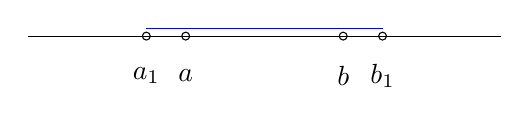
\begin{tikzpicture}
	\draw (-3,0) -- (3,0);
	\draw[blue] (-1.5,0.1) -- (1.5,0.1);
	\draw (-1,0) circle (0.05cm);
	\draw (-1,-0.5) node{$a$};
	\draw (1,0) circle (0.05cm);
	\draw (1,-0.5) node{$b$};

	\draw (-1.5,0) circle (0.05cm);
	\draw (-1.5,-0.5) node{$a_1$};
	\draw (1.5,0) circle (0.05cm);
	\draw (1.5,-0.5) node{$b_1$};
\end{tikzpicture}
\end{center}

	Suppose $b_1 < b$.
	Clearly, $a < b_1$.
	And the cover $\mathcal{C}$ must have an open interval containing $b_1$.
	Otherwise $\mathcal{C}$ is not a cover of $[a,b]$.
	That is, there exists $(a_2,b_2)$ containing $b_1 \in (a,b)$ such that $a_2 < b_1 < b_2$.
	If $b_2 > b$, then $\displaystyle \sum_{i=1}^k l(I_k) \ge l(a_1,b_1) + l(a_2,b_2) \ge l(a_1,b_2) \ge b-a$.

\begin{center}
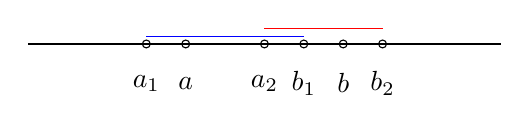
\begin{tikzpicture}
	\draw (-3,0) -- (3,0);
	\draw (-1,0) circle (0.05cm);
	\draw (-1,-0.5) node{$a$};
	\draw (1,0) circle (0.05cm);
	\draw (1,-0.5) node{$b$};

	\draw (-1.5,0) circle (0.05cm);
	\draw (-1.5,-0.5) node{$a_1$};
	\draw (0.5,0) circle (0.05cm);
	\draw (0.5,-0.5) node{$b_1$};
	\draw[blue] (-1.5,0.1) -- (0.5,0.1);

	\draw (0,0) circle (0.05cm);
	\draw (0,-0.5) node{$a_2$};
	\draw (1.5,0) circle (0.05cm);
	\draw (1.5,-0.5) node{$b_2$};
	\draw[red] (0,0.2) -- (1.5,0.2);
\end{tikzpicture}
\end{center}

	Suppose $b_2 < b$.
	Continuing like this we get, $N$ open intervals in $\mathcal{C}$, $\{ (a_k,b_k) : k = 1,2,\cdots,N \} $ such that $a_1 < a < b_1$ and $a_N < b < b_N$ and $a_k < b_{k-1} < b_k$ for all $k$.
	The process should terminate in finite steps as $\mathcal{C}$ is a finite cover of $[a,b]$.
	Then $\displaystyle \sum_{k=1}^N l(I_k) \ge \sum_{k=1}^N l(a_k,b_k) \ge l(a_1,b_N) \ge b-a$.

\begin{center}
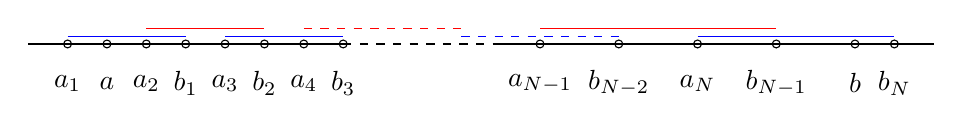
\begin{tikzpicture}
	\draw (-5,0) -- (-1,0);
	\draw[dashed] (-1,0) -- (1,0);
	\draw (1,0) -- (6.5,0);

	\draw (-4,0) circle (0.05cm);
	\draw (-4,-0.5) node{$a$};
	\draw (5.5,0) circle (0.05cm);
	\draw (5.5,-0.5) node{$b$};

	\draw (-4.5,0) circle (0.05cm);
	\draw (-4.5,-0.5) node{$a_1$};
	\draw (-3,0) circle (0.05cm);
	\draw (-3,-0.5) node{$b_1$};
	\draw[blue] (-4.5,0.1) -- (-3,0.1);

	\draw (-3.5,0) circle (0.05cm);
	\draw (-3.5,-0.5) node{$a_2$};
	\draw (-2,0) circle (0.05cm);
	\draw (-2,-0.5) node{$b_2$};
	\draw[red] (-3.5,0.2) -- (-2,0.2);

	\draw (-2.5,0) circle (0.05cm);
	\draw (-2.5,-0.5) node{$a_3$};
	\draw (-1,0) circle (0.05cm);
	\draw (-1,-0.5) node{$b_3$};
	\draw[blue] (-2.5,0.1) -- (-1,0.1);
	
	\draw (-1.5,0) circle (0.05cm);
	\draw (-1.5,-0.5) node{$a_4$};
	\draw[red,dashed] (-1.5,0.2) -- (0.5,0.2);

	\draw (2.5,0) circle (0.05cm);
	\draw (2.5,-0.5) node{$b_{N-2}$};
	\draw[blue,dashed] (0.5,0.1) -- (2.5,0.1);

	\draw (1.5,0) circle (0.05cm);
	\draw (1.5,-0.5) node{$a_{N-1}$};
	\draw (4.5,0) circle (0.05cm);
	\draw (4.5,-0.5) node{$b_{N-1}$};
	\draw[red] (1.5,0.2) -- (4.5,0.2);

	\draw (3.5,0) circle (0.05cm);
	\draw (3.5,-0.5) node{$a_N$};
	\draw (6,0) circle (0.05cm);
	\draw (6,-0.5) node{$b_N$};
	\draw[blue] (3.5,0.1) -- (6,0.1);
\end{tikzpicture}
\end{center}

	Clearly, every open cover of $[a,b]$ contains a finite subcover $\mathcal{C}$, which contains a finite subcover of the form $\{ (a_k,b_k) : k=1,2,\cdots,N \}$ such that $\displaystyle \sum_{k=1}^N l(I_k) \ge b-a$.
	Thus, for any open cover $\displaystyle \sum_{k=1}^\infty l(I_k) \ge b-a$.
	And thus,
	\begin{equation}
		m^\ast([a,b]) \ge b-a
	\end{equation}

	\textbf{Case 2 : Bounded Interval}
	Let $I$ be a bounded interval.
	Then there exists bounded closed intervals $J_1$ and $J_2$ such that $J_1 \subsetneq I \subsetneq J_2$ such that $l(I) - \varepsilon < l(J_1)$ and $l(J_2) < l(I)+\varepsilon$.
	Suppose $I = (a,b]$, then $J_1 = [a+\frac{\varepsilon}{2}, b-\frac{\varepsilon}{2}]$ and $J_2 = [a-\frac{\varepsilon}{2},b+\frac{\varepsilon}{2}]$.\\

	By monotonicity of Lebesgue outer measure, we have $m^\ast(J_1) \le m^\ast(I) \le m^\ast(J_2)$.
	However $m^\ast(J_1) = l(I)-\varepsilon$ and $m^\ast(J_2) = l(I)+\varepsilon$.
	Thus, $l(I)-\varepsilon \le m^\ast(I) \le l(I)+\varepsilon$.
	Therefore, $m^\ast(I) = l(I)$.

	\textbf{Case 3 : Unbounded Interval}
	Let $I$ be an unbounded interval.
	Then for any natural number $n$, there exists a closed bounded interval $J$ such that $J \subset I$ and $l(J) = n$.
	And $n = m^\ast(J) \le m^\ast(I),\ \forall n \in \mathbb{N}$.
	Therefore, $m^\ast(I) = \infty = l(I)$. 
	\end{proof}
	\item Outer Measure is translation invariant
	\begin{proof}
	Let $A$ be any set and $y \in \mathbb{R}$.
	Let $\{ I_k : k = 1,2,\dots \}$ be a cover of $A$.
	Then $\{ I_k+y : k = 1,2,\dots \}$ is a cover of $A+y$.
	And $l(I_k) = l(I_k+y)$ for every natural number $k$ and real number $y$.
	Thus, $\displaystyle \sum_{k=1}^\infty l(I_k) = \sum_{k=1}^\infty l(I_k+y)$.
	Clearly, for each cover $\{I_k\}_{k=1}^\infty$ of $A$, there exists a cover $\{ I_k+y \}_{k=1}^\infty$ of $A+y$ containing intevals of same length.
	Therefore, $m^\ast(A) = m^\ast(A+y)$.
	\end{proof}
	\item Outer Measure is countably subadditive
	\begin{proof}
	Let $\{E_k\}_{k=1}^\infty$ be a countable collection of sets.
	It is enough to prove that
		\begin{equation}
			m^\ast \left( \bigcup_{k=1}^\infty E_k \right) \le \sum_{k=1}^\infty m^\ast(E_k)
		\end{equation}
		For each natural number $k$, we have a cover of $E_k$, say $\{ I_{k,i} \}_{i = 1}^\infty$ such that $\displaystyle \sum_{i=1}^\infty l(I_{k,i}) < m^\ast(E_k) + \frac{\varepsilon}{2^k}$.
		Suppose that, for some $\varepsilon > 0$, $E_k$ doesn't have such a cover, then $m^\ast(E_k) + \frac{\varepsilon}{2^k}$ is an upper bound contradicting the assumption that $m^\ast(E_k)$ is the least upper bound.\\

	Clearly,
`	\begin{align*}
	m^\ast \left( \bigcup_{i,k = 0}^\infty I_{k,i} \right)
	\le & \sum_{k=1}^\infty \sum_{i=1}^\infty l(I_{k,i}) \\
	= & \sum_{k=1}^\infty \left( m^\ast(E_k) + \frac{\varepsilon}{2^k} \right) \\
	= & \sum_{k=1}^\infty  m^\ast(E_k) + \varepsilon
	\end{align*}
\end{proof}
	\textbf{Note : } Finite subadditivity is a weaker notion than countable subadditivity.
	Since every finite collection is a countable collection.
\end{enumerate}

\subsubsection{Exercise}
\begin{enumerate}
	\setcounter{enumi}{4}
\item Closed Interval $[0,1]$ is uncountable.\\
	Suppose $[0,1]$ is countable, then Lebesgue outer measure of any countable set is zero, $m^\ast([0,1]) = 0$.
		But, $[0,1]$ is an interval and Lebesgue outer measure of an interval is its length, $m^\ast([0,1]) = l([0,1]) = 1$ which is a contradiction.
\item $m^\ast([0,1] - \mathbb{Q}) = 1$
	\[ [0,1] = \left( [0,1] \cap \mathbb{Q} \right)\ \cup\ \left( [0,1]\cap \mathbb{Q}^c \right) \]
	Clearly, $m^\ast([0,1]) = 1$.
		And $[0,1] \cap \mathbb{Q}$ is a countable set since $\mathbb{Q}$ is countable.
		And thus has Lebesgue outer measure zero.
		Thus by countable subadditivity, we have
		\[ 1 = m^\ast([0,1]) \le m^\ast([0,1] \cap \mathbb{Q}^c) + 0 \]
		Thus, $m^\ast([0,1] \cap \mathbb{Q}^c) \ge 1$.
		And $[0,1] \cap \mathbb{Q}^c\ \subset [0,1]$.
		By monotonicity, $m^\ast([0,1] \cap \mathbb{Q}^c) \le m^\ast([0,1]) = 1$.
		Therefore, $m^\ast([0,1] \cap \mathbb{Q}^c) = 1$.
	\item Construction of a $G_\delta$ set containing $E$ % hint : $G_\delta = \cup_{k=1}^\infty F_k$ where
	\item hint : if sum of interval is less than 1.
		Then it is not a cover of $[0,1]$.
	\item hint : $A \cup B = A \cup (B-A) = A \cup (B \cap A^c)$
	\item hint : $A$ and $B$ are separated by distance $\alpha$, thus are disjont.
\end{enumerate}

\subsection{$\sigma$-algebra of Lebesgue Measurable Sets}
	Lebesgue Outer Measure is defined for any subset of real numbers and Lebesgue outer measure of an interval is its length.
	However, it isn't countable additive.\\

	There exists disjoint sets $A,B$ such that $m^\ast(A\cup B) < m^\ast(A)+m^\ast(B)$.\\
	
	Since countable additivity is a favourable property over countable subadditivity.
	We restrict the family of subsets of real numbers to those subsets that allow countable additivity.
	
\subsubsection{Lebesgue Measurable Set}
\begin{definition}[Measurable Set]
	Let $E$ be a subset of $\mathbb{R}$.
	Then $E$ is Lebesgue measurable if
\begin{equation}
	m^\ast(A) = m^\ast(A \cap E) + m^\ast(A \cap E^c)
	\label{eq:measurable1}
\end{equation}
	for any subset $A$ of $\mathbb{R}$.
\end{definition}

	In other words, $E$ is Lebesgue measurable if $E$ doesn't affect countable additivity of Lebesgue Outer Measure.\\

	We will consider only those subset of real numbers, which won't affect countable additivity.
	These subsets are \textbf{Lebesgue Measurable}.
	And we could show that the collection of all Lebesgue Measurable sets forms a $\sigma$-algebra.
	Clearly, intervals allow countable additivity, thus the Borel Algebra is contained in this $\sigma$-algebra of Lebesgue measurable sets.
\subsubsection{Simplified Condition for Lebesgue Measurability}

We know that Lebesgue Outer Measure has countable subadditivity.
\begin{equation*}
	m^\ast(A) \le m^\ast(A \cap E) + m^\ast(A \cap E^c)
\end{equation*}
Thus, for condition (\ref{eq:measurable1}), it is sufficient to check the following condition,
\begin{equation}
	m^\ast(A) \ge m^\ast(A \cap E) + m^\ast(A \cap E^c)
	\label{eq:measurable2}
\end{equation}

\subsubsection{Properties of Lebesgue Measure}
\begin{enumerate}
	\item Any set of Lebesgue outer measure zero is Lebesgue measurable.
	\begin{proof}
		Let $E$ be a subset of real numbers with Lebesgue outer measure zero.
		Let $A$ be any subset of real numbers.
		Then $A = (A \cap E) \cup (A \cap E^c)$.
		By countable additivity, $m^\ast(A) \le m^\ast(A \cap E) + m^\ast(A \cap E^c)$.
		Since $A\cap E \subset E$, we have by monotonicity $m^\ast(A \cap E) \le m^\ast(E) = 0$.\\


		Again, $A \cap E^c \subset A$ and by monotonicity, $m^\ast(A) \ge m^\ast(A \cap E^c) = 0+m^\ast(A \cap E^c) = m^\ast(A\cap E) + m^\ast(A \cap E^c)$.
		Thus, $E$ is Lebesgue measurable by the simplified condition for Lebesgue measurability.
	\end{proof}

	\item Countable sets are Lebesgue measurable.
	\begin{proof}
	Countable sets are of Lebesgue outer measure zero.
	And sets of Lebesgue outer measure zero are Lebesgue measurable.
	Thus, they are Lebesgue measurable.
	\end{proof}
	\item Finite union of Lebesgue measurable sets is Lebesgue measurable.
		\label{thm:finiteunionmeasurable}
	\begin{proof}
		It is enough to prove that if $E_1$ and $E_2$ are Lebesgue measurable, then their union is also Lebesgue measurable.
		Then, by finite mathematical induction, we can prove that the result if true for any finite collection of Lebesgue measurable sets.\\


	Suppose $E_1, E_2$ are Lebesgue measurable sets.
	Since $E_1$ is Lebesgue measurable,
	\begin{equation}
		m^\ast(A) = m^\ast(A \cap E_1) + m^\ast(A \cap E_1^c)
	\end{equation}
	And consider $A \cap E_1^c$ instead of $A$.
	Since $E_2$ is Lebesgue measurable, we get
	\begin{equation}
		m^\ast(A \cap E_1^c) = m^\ast(A \cap E_1^c\cap  E_2) + m^\ast(A \cap E_1^c \cap E_2^c)
	\end{equation}

	We have $(A \cap E_1^c) \cap E_2^c = A \cap (E_1^c \cap E_2^c) = A \cap (E_1 \cup E_2)^c$.
	And $(A \cap E_1) \cup (A \cap E_1^c \cap E_2) = (A \cap E_1) \cup [A \cap (E_2 \cap E_1^c)] = A \cap (E_1 \cup E_2)$.
\begin{center}
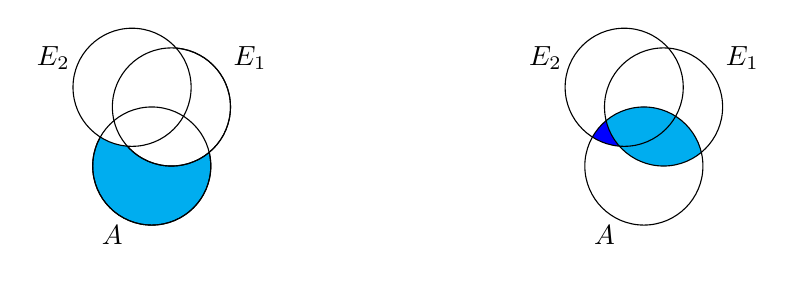
\begin{tikzpicture}[scale=0.25]
	\filldraw[fill = cyan] (0,-1.5) circle (3cm);
	\filldraw[fill = white] (1,1.5) circle (3cm);
	\filldraw[fill = white] (-1,2.5) circle (3cm);
	\draw (0,-1.5) circle (3cm);
	\draw (1,1.5) circle (3cm);
	\draw (-2,-5) node{$A$};
	\draw (5,4) node{$E_1$};
	\draw (-5,4) node{$E_2$};

	\begin{scope}
		\clip (25,-1.5) circle (3cm);
		\fill[blue] (24,2.5) circle (3cm);
	\end{scope}
	\begin{scope}
		\clip (25,-1.5) circle (3cm);
		\fill[cyan] (26,1.5) circle (3cm);
	\end{scope}
	\draw (25,-1.5) circle (3cm);
	\draw (26,1.5) circle (3cm);
	\draw (24,2.5) circle (3cm);
	\draw (23,-5) node{$A$};
	\draw (30,4) node{$E_1$};
	\draw (20,4) node{$E_2$};
\end{tikzpicture}
\end{center}
	\begin{align*}
		m^\ast(A) = & m^\ast(A \cap E_1) + m^\ast(A \cap E_1^c) \\
		= & {\color{blue}m^\ast(A \cap E_1) + m^\ast(A \cap E_1^c \cap E_2)} + m^\ast(A \cap E_1^c \cap E_2^c) \\
		\ge & {\color{blue}m^\ast[A \cap (E_1 \cup E_2)]} + m^\ast[A \cap (E_1 \cup E_2)^c] 
	\end{align*}
	Therefore $E_1 \cup E_2$ is Lebesgue measurable.
		And by finite induction, finite union of Lebesgue measurable sets is also Lebesgue measurable.
	\end{proof}

	\item Lebesgue Measure is finitely additive.\\
		In other words, Suppose $\{E_k\}_{k = 1}^n$ be a finite collection of disjoint, Lebesgue measurable sets.
		Then Lebesgue measure of their union is the sum of Lebesgue measures.
	\begin{proof}
	Let $A$ be any subset of $\mathbb{R}$ and $\{ E_k \}_{k=1}^n$ be a finite collection of disjoint, Lebesgue measurable subsets of $\mathbb{R}$.
	\begin{equation}
		\text{Claim : }	m^\ast \left( A \cap \left[ \bigcup_{k=1}^\infty E_k\right] \right) = \sum_{k=1}^\infty m^\ast (A \cap E_k)
	\end{equation}
	Trivially, the claim is true for $n=1$.
		Suppose the claim is true for $n-1$.
		That is,
	\begin{equation}
		m^\ast \left( A \cap \left[ \bigcup_{k=1}^{n-1} E_k \right] \right) = \sum_{k=1}^{n-1} m^\ast (A \cap E_k)
	\end{equation}
	From set theory we have,
	\begin{align}
		A \cap \left[ \bigcup_{k=1}^n E_k \right] \cap E_n & = A \cap E_n\\
		A \cap \left[ \bigcup_{k=1}^n E_k \right] \cap E_n^c  & = A \cap \left[ \bigcup_{k=1}^{n-1} E_n \right]
	\end{align}
	By Lebesgue measurability of $E_n$, we have
	\begin{align*}
		m^\ast \left( A \cap \left[ \bigcup_{k=1}^n E_k \right] \right) = & m^\ast \left( A \cap \left[ \bigcup_{k=1}^n E_k \right] \cap E_n \right) + m^\ast \left( A \cap \left[ \bigcup_{k=1}^n E_k \right] \cap E_n^c \right)\\
		& = m^\ast \left( A \cap E_n \right) + m^\ast  \left( A \cap \left[ \bigcup_{k=1}^{n-1} E_n \right] \right) \\
		& =  \sum_{k=1}^n m^\ast \left( A \cap E_k \right) \text{, by mathematical induction}
	\end{align*}
	Taking $A = \mathbb{R}$, we get Lebesgue measure is finitely additive.
		That is,
	\begin{equation}
		m^\ast \left( \bigcup_{k=1}^n E_k \right) = \sum_{k=1}^n m^\ast \left( E_k \right)
	\end{equation}
	\end{proof}
\item Countable union of Lebesgue measurable sets is Lebesgue measurable
	\label{thm:countableunionmeasurable}
	\begin{proof}
		Let $A$ be any subset of $\mathbb{R}$.
		And $\{ E_k \}_{k=1}^\infty$ be a countable collection of disjoint, Lebesgue measurable subsets of $\mathbb{R}$.
		Define $F_n = \cup_{k=1}^n E_k$ and $E = \cup_{k=1}^\infty E_k$.
		Clearly, $F \subset E$ and $F^c \supset E^c$.
		Thus, $m^\ast(A \cap F_n^c) \ge m^\ast(A \cap E^c)$.
	\begin{align*}
		m^\ast(A) & =  m^\ast (A \cap F_n) + m^\ast (A \cap F_n^c) \\
		& \ge m^\ast \left( A \cap \left[ \bigcup_{k=1}^n E_k \right] \right) + m^\ast(A \cap E^c) \\
		& \ge \sum_{k=1}^n m^\ast(A \cap E_k) + m^\ast(A \cap E^c) 
	\end{align*}
	\begin{align*}
		\lim_{n \to \infty} m^\ast(A) & \ge \lim_{n \to \infty} \sum_{k=1}^n m^\ast(A \cap E_k) + m^\ast(A \cap E^c) \\
		m^\ast(A) & \ge \sum_{k=1}^\infty m^\ast(A \cap E_k) + m^\ast (A \cap E^c) \\
		& \ge m^\ast \left( A \cap \left[ \bigcup_{k=1}^\infty E_k \right] \right) + m^\ast(A \cap E^c) \\
		\implies m^\ast(A) & \ge m^\ast (A \cap E) + m^\ast(A \cap E^c)
	\end{align*}
		By above inequality, $E = \cup_{k=1}^\infty E_k$ is Lebesgue measurable.\\

		And, any countable collection of Lebesgue measurable sets can be expressed as a countable collection of disjoint, Lebesgue measurable sets.
		Let $\{ E_k \}_{k=1}^\infty$ be a collection of Lebesgue measurable sets.
		Then, the countable collection, $\{ E_k' \}_{k=1}^\infty$ defined by $E_k'= E_k - \cup_{j=1}^{k-1}E_k$ contains disjoint, Lebesgue measurable\dag\footnote{
			Suppose $E_1,E_2$ are measurable, then $E_2^c = \mathbb{R} - E_2$ is measurable by the duality of measurability condition.
		And $E_1 \cap E_2^c = E_1-E_2$ is Lebesgue measurable since countable intersection of Lebesgue measurable sets is Lebesgue measurable (by Property 4 and de Morgan's Law).}
	subsets of $\mathbb{R}$.
		Therefore, countable union of Lebesgue measurable sets is Lebesgue measurable.
	\end{proof}
	\item Every interval is Lebesgue measurable.
	\begin{proof}
	It is sufficient to prove that $(a,\infty)$ is Lebesgue measurable.
	Suppose $(a,\infty)$ is Lebesgue measurable for every $a \in \mathbb{R}$.
	Then interval $(a,b)$ is Lebesgue measurable, since $(a,b) = [(a,\infty) \cap (\mathbb{R}-(b,\infty))]-\{b\}$.\\


	Let $A$ be any subset of $\mathbb{R}$.
	Define $A_1 = A\cap (-\infty,a)$ and $A_2 = A \cap (a,\infty)$ such that $A-\{a\} = A_1 \cup A_2$ and $A_1 \cap A_2 = \phi$.
	And the interval $(a,\infty)$ is Lebesuge measurable only if 
	\begin{equation}
		m^\ast(A) \ge m^\ast(A \cap (a,\infty)) + m^\ast(A \cap (a,\infty)^c) = m^\ast(A_1)+m^\ast(A_2)
		\dag\footnote{We have, $m^\ast(A \cap (-\infty,a]) = m^\ast(A \cap (-\infty,a)$ since removing finite number of points from a subset of $\mathbb{R}$ won't affect its Lebesgue measure.}
	\end{equation}
	Let collection $\{ I_k \}_{k=1}^\infty$ be a countable cover of $A$.
		Then collection $\{ I_k' \}_{k=1}^\infty$ defined by $I_k' = I_k \cap (a,\infty)$ is a cover of $A_1$.
		And collection $\{I_k''\}_{k=1}^\infty$ defined by $I_k'' = I_k \cap (-\infty,a)$ is a cover of $A_2$.\\

	Clearly, $\displaystyle m^\ast(A_1) \le \sum_{k=1}^\infty l(I_k')$ and $\displaystyle m^\ast(A_2) \le \sum_{k=1}^\infty l(I_k'')$.
	\begin{align*}
		m^\ast(A_1)+m^\ast(A_2) & \le \sum_{k=1}^\infty l(I_k') + \sum_{k=1}^\infty l(I_k'') \\
		& \le \sum_{k=1}^\infty l(I_k') + l(I_k'') \\
		& \le \sum_{k=1}^\infty l(I_k) \le m^\ast(A)
	\end{align*}
		Thus, $(a,\infty)$ is Lebesgue measurable.
		Therefore, every interval is Lebesgue measurable.
	\end{proof}
	\item $\sigma$-algebra of Lebesgue measurable sets $\mathcal{M}$ contains Borel Sets $\mathcal{B}$.
	\begin{equation}
		\mathcal{B} \subset \mathcal{M}
	\end{equation}
	\begin{proof}
	The Borel algebra $\mathcal{B}$ is the $\sigma$-algebra containing all intervals.
		We have proved that, every intervals are Lebesgue measurable.
		Also, we have proved that the set of all Lebesgue measurable subsets of $\mathbb{R}$ is a $\sigma$-algebra as complements of Lebesgue measurable sets are Lebesgue measurable by duality of the condition and countable union of Lebesgue measurable sets are also Lebesgue measurable.
		Therefore, every Borel set is Lebesgue measurable.
		Clearly, $G_\delta$ and $F_\sigma$ are Borel sets and are Lebesgue measurable.
	\end{proof}
	\item Lebesgue Measurability is translation invariant.
	\begin{proof}
		Let $E$ be a Lebesgue measurable set.
		Let $A$ be any subset of $\mathbb{R}$ and $y \in \mathbb{R}$.
		Then,
	\begin{align*}
		m^\ast(A) & = m^\ast(A-y)\\
		& = m^\ast((A-y) \cap E) + m^\ast((A-y) \cap E^c)\\
		& = m^\ast(A \cap (E+y)) + m^\ast(A \cap (E+y)^c)
	\end{align*}
		Thus, $E+y$ is Lebesgue measurable.
		And Lebesgue measurability is traslation invariant.
	\end{proof}
\end{enumerate}

\subsubsection{Exercise}
\begin{enumerate}
	\setcounter{enumi}{10}
	\item Let $\mathcal{A}$ be the $\sigma$-algebra containing all intervals of the form $(a, \infty)$.
		Every interval has one of the four forms,
	\begin{align}
		(a,b] = & (a,\infty) \cap (b,\infty)^c \\
		(a,b) = & (a,\infty) \cap \left[\bigcap_{k=1}^\infty \left(b-\frac{1}{k},\infty\right)\right]^c \\
		[a,b] = & \left[ \bigcap_{k=1}^\infty \left(a-\frac{1}{k},\infty\right)\right] \cap (b,\infty)^c \\
		[a,b) = & \left[\bigcap_{k=1}^\infty \left(a-\frac{1}{k},\infty\right)\right] \cap \left[ \bigcap_{k=1}^\infty \left(b-\frac{1}{k},\infty\right)\right]^c
	\end{align}
\item \textbf{Borel sets} is the $\sigma$-algebra containing all open intervals.
	The equations from previous equations are sufficient.
	However, we have a simpler form for closed intervals, $[a,b]$.
	\begin{align}
		[a,b] = & \left[(-\infty,a) \cup (b,\infty) \right]^c 
	\end{align}
		Clearly, every interval is a Borel set.
	\item
	\begin{itemize}
		\item $C \in F_\sigma \implies C = \bigcup_{k=1}^\infty C_k \implies \bigcup_{k=1}^\infty \left(C_k+y\right) = C+y \in F_\sigma$
		\item $O \in G_\delta \implies O = \bigcap_{k=1}^\infty O_k \implies \bigcup_{k=1}^\infty \left( O_k+y \right) =  O+y \in G_\delta$
		\item $m^\ast(E) = 0 \implies 0 = \inf\{\sum_{k=1}^\infty l(I_k)\} = \inf\{\sum_{k=1}^\infty l(I_k+y)\} \implies  m^\ast(E+y) = 0$
	\end{itemize}
	\item A subset $E$ has positive Lebesgue measure if and only if it has a bounded subset of positive Lebesgue measure.
		\[ m^\ast(E) > 0 \iff \exists \text{ bounded subset }F \subset E,\text{ such that } m^\ast(F) > 0 \]
		\textbf{Sufficient Part :} By monotonicity, $F \subset E \implies m^\ast(F) \le m^\ast(E)$.
		And $m^\ast(F) > 0 \implies 0 < m^\ast(F) \le m^\ast(E)$.\\
		\textbf{Necessary Part :}
	\item 
\end{enumerate}

\subsection{Outer and Inner Approximation}
\begin{definition}[Excision Property]
Let $A$ be a Lebesgue measurable set of finite measure and $A \subset B$.
	Then,
\begin{equation}
	m^\ast(B \sim A) = m^\ast(B) - m^\ast(A)
\end{equation}
\begin{proof}
\begin{align*}
	m^\ast(B) = & m^\ast(B \cap A) + m^\ast(B \cap A^c) \\
	= & m^\ast(A) + m^\ast(B \sim A) \\
	\implies m^\ast(B \sim A) = & m^\ast(B) - m^\ast(A)
\end{align*}
\end{proof}
\end{definition}

\begin{theorem}[approximation]
	The following conditions are equivalent to Lebesgue measurability of $E$
\begin{enumerate}
	\item $\forall \varepsilon > 0$, there is an open set $\mathcal{O}$ containing $E$ for which $m^\ast(\mathcal{O}\sim E) < \varepsilon$.
	\item There is a $G_\delta$ set $G$ containining $E$ such that $m^\ast(G \sim E) = 0$.
	\item $\forall \varepsilon > 0$, there is a closed set $F$ contained in $E$ such that $m^\ast(E\sim F) {\color{red}<} 0$.
	\item There is an $F_\sigma$ set $F$ contained in $E$ sucht hat $m^\ast(E \sim F) = 0$.
\end{enumerate}
\end{theorem}

\textbf{Note :} Equivalent conditions 1 \& 2 are about outer approximation of a Lebesgue measurable set and 3 \& 4 are about inner approximation of a Lebesgue measurable set.\\

\begin{proof}
\subsubsection*{Measurability $\implies$ Open set - Outer approximation}
	Suppose that $E$ is Lebesgue measurable.
	And let $\varepsilon > 0$.\\


	\textbf{Case 1 :} Suppose $m^\ast(E) < \infty$.
	By definition of Lebesgue outer measure, there exists an open cover $\{ I_k \}_{k=1}^\infty$ such that $\displaystyle \sum_{k=1}^\infty l(I_k) <  m^\ast(E)+\varepsilon$.\\

	Define $\mathcal{O} = \displaystyle \bigcup_{k=1}^\infty I_k$.
	Then $\mathcal{O}$ is an open set containing $E$ and thus Lebesgue measurable.
	Also, $\displaystyle m^\ast(\mathcal{O}) \le \sum_{k=1}^\infty l(I_k) < m^\ast(E) + \varepsilon$.
	Therefore, by excision property we have $m^\ast(\mathcal{O} \sim E) = m^\ast(\mathcal{O}) - m^\ast(E) < \varepsilon$. \\

	\textbf{Case 2 :} Suppose $m^\ast(E) = \infty$.
	Without loss of generality, $E$ may be written as countable union Lebesgue measurable sets $\{ E_k \}_{k=1}^\infty$ of finite measure.\\

	By case 1, for every $k$, there exists $\mathcal{O}_k$ for each $E_k$ of finite measure such that $m^\ast(\mathcal{O}_k \sim E_k) < \frac{\varepsilon}{2^k}$.
	Define $\displaystyle \mathcal{O} = \bigcup_{k=1}^\infty \mathcal{O}_k$.
	Then $\mathcal{O}$ is open, contains $E$ and 
	\begin{align*}
		m^\ast(\mathcal{O} \sim E) = & m^\ast\left(\bigcup_{k=1}^\infty \mathcal{O}_k \sim E \right) \\
		\le & m^\ast \left(\bigcup_{k=1}^\infty \mathcal{O}_k \sim E_k \right) \\
		\le & \sum_{k=1}^\infty m^\ast(\mathcal{O}_k \sim E_k) = \varepsilon \sum_{k=1}^\infty \frac{1}{2^k} = \varepsilon
	\end{align*}

\subsubsection*{Open, Outer approximation $\implies G_\delta$, Outer approximation }
	Let $E$ be a subset of real numbers such that Lebesgue measure of $E$ has an open set inner approximation.
	That is, for every $\varepsilon > 0$, there exists an open set $\mathcal{O}$ such that $m^\ast(\mathcal{O} \sim E) < \varepsilon$.\\

	Let $\mathcal{O}_k$ be open sets such that $m^\ast(\mathcal{O}_k \sim E) < \frac{1}{k}$.
	Define $\displaystyle G = \bigcap_{k=1}^\infty \mathcal{O}_k$.
	Then, $G$ is a $G_\delta$ set containing $E$.
	And $G \sim E \subset \mathcal{O}_k \sim E$.
	Thus, by monotonicity, $m^\ast(G \sim E) \le m^\ast(\mathcal{O}_k \sim E) < \frac{1}{k}$.
	Thus, we have a $G_\delta$ set $G$ containing $E$ such that $m^\ast(G \sim E) = 0$.

\subsubsection*{$G_\delta$-Outer approximation $\implies$ Measurability}
	We have, $m^\ast(G \sim  E) = 0$.
	Since every set of Lebesgue measure zero is Lebesgue measurable, $G \sim E$ is Lebesgue measurable.
	And its complement $(G \sim E)^c$ is also Lebesgue measurable.
	Also we have, $G$ is a $G_\delta$ set, thus a Borel set and hence Lebesgue measurable.\\

	Clearly,we have $E = G \cap (G \sim E)^c$.
	And therefore, $E$ is Lebesgue measurable.

\subsubsection*{Open, Outer approximation $\iff$ Closed, Inner approximation}
	By duality of Lebesgue measurability, $E$ is Lebesgue measurable if and only if $E^c$ is Lebesgue measurable.
	And by de Morgan's Law, we have $E^c$ has an open set - outer approximation $\mathcal{O}$ if and only if $E$ has a closed set - inner approximation $\mathcal{O}^c$.
	\[ m^\ast(\mathcal{O} \sim E^c) < \varepsilon \iff m^\ast(E \sim \mathcal{O}^c) < \varepsilon \]

\subsubsection*{$G_\delta$-Outer approximation $\iff F_\sigma$-Inner approximation}
	Again, by duality of Lebesgue measurability and de Morgan's Law, we have $E^c$ has a $G_\delta$-outer approximation $G$ if and only if $E$ has an $F_\sigma$-inner approximation $F$.
	\[ m^\ast(G \sim E^c) {\color{red}= 0} \iff m^\ast(E \sim F){\color{red} = 0} \]
\end{proof}

\begin{theorem}
	Let $E$ be a Lebesgue measurable set of finite measure.
	Then for any $\varepsilon > 0$, there exists a finite collection of disjoint open sets $\{ I_k \}_{k=1}^n$ such that  $\displaystyle \mathcal{O} = \bigcup_{k=1}^n I_k$ and $m^\ast(\mathcal{O} \sim E) + m^\ast(E \sim \mathcal{O}) < \varepsilon$.
\end{theorem}
\begin{proof}
	Since $E$ is Lebesgue measurable, by outer approximation theorem we have an open set $U$ such that $E \subset U$ and 
	\begin{equation*}
		m^\ast(U \sim E) < \frac{\varepsilon}{2}
	\end{equation*}

	\begin{align*}
		U =  & (U \cap E) \cup (U \cap E^c)
		\intertext{Since $E$ is Lebesgue measurable, $m^\ast(E) < k$}
		m^\ast(U) = &  m^\ast(U \cap E) + m^\ast(U \cap E^c) \\
		= & m^\ast(E) + m^\ast(U \sim E)
		\intertext{Since $E$ has finite measure}
		m^\ast(U) = & m^\ast(E) + m^\ast(U \sim E) \\
		< & k+\frac{\varepsilon}{2} < \infty
	\end{align*}
	That is, $U$ is of finite measure. \\

	Since $U$ is open, $U$ is countable\dag\footnote{
		By definition, \textbf{Open sets} are countable union of disjoint, open intervals}
	union of a disjoint collection of open intervals, say $\{ I_k \}_{k=1}^\infty$. Clearly,
	\begin{align*}
		\sum_{k=1}^n l(I_k) & \le \sum_{k=1}^\infty {\color{red}l(I_k)} \le m^\ast(U) < \infty 
		%\sum_{k=1}^\infty l(I_k) & < \infty  %% not required
		\intertext{ By characterisation of series convergence, there exists an integer $n$ such that,}
		\sum_{k=n+1}^\infty l(I_k) & < \frac{\varepsilon}{2}
	\end{align*}
	Define $\displaystyle \mathcal{O} = \bigcup_{k=1}^n I_k$.
	Since $\mathcal{O} \sim E \subset U \sim E$, by monotonicity we have 
	\begin{equation}
		m^\ast(\mathcal{O} \sim E) \le m^\ast(U \sim E) < \frac{\varepsilon}{2}
	\end{equation}

	Since $E \subset U$, we have $\displaystyle E \sim \mathcal{O} \subset U \sim \mathcal{O} = \bigcup_{k=1}^n I_k$.
	And clearly, 
	\begin{equation*} 
		U \sim \mathcal{O} = \bigcup_{k=1}^\infty I_k \sim \bigcup_{k=1}^n I_k\ {\color{red}\subseteq} \bigcup_{k=n+1}^\infty I_k
	\end{equation*}
	\begin{align}
		\text{Thus, } m^\ast(E \sim \mathcal{O}) \le & m^\ast(U \sim \mathcal{O}) \le \sum_{k=n+1}^\infty l(I_k) < \frac{\varepsilon}{2} 
		\intertext{Therefore,}
		m^\ast(E \sim \mathcal{O}) + m^\ast(\mathcal{O} \sim E) < & \varepsilon \nonumber
	\end{align}
\end{proof}

\subsubsection{Exercise}

\begin{enumerate}
	\setcounter{enumi}{16}
\item Let $\varepsilon > 0$ and $E$ is Lebesgue measurable.
	Then there exists open set $\mathcal{O}$ and closed set $F$ such that $F \subset E \subset \mathcal{O}$, $m^\ast(E \sim F) < \frac{\varepsilon}{2}$ and $m^\ast(\mathcal{O} \sim E) < \frac{\varepsilon}{2}$.
	Clearly, $\mathcal{O} \sim E$ and $E \sim F$ are disjoint and $\mathcal{O} \sim F = (\mathcal{O} \sim E) \cup (E \sim F)$.
		Thus by monotonicity of Lebesgue outer measure, we have $m^\ast(\mathcal{O} \sim F) \le m^\ast(\mathcal{O} \sim E) + m^\ast(E \sim F) < \varepsilon$.
\item
 Suppose $E$ has finite outer measure.
	\dag\footnote{
		$E$ has finite outer measure does not imply $E$ is bounded or Lebesgue measurable.}\\
	\textbf{$G_\delta$ set : }
	Let $\varepsilon > 0$.
	Then by the definition of Lebesgue outer measure, there exists a cover $\{ I_k \}_{k=1}^\infty$ of $E$ such that $\displaystyle \sum_{k=1}^\infty l(I_k) < m^\ast(E) - \frac{\varepsilon}{2}$.
	Define $\displaystyle G = \bigcup_{k=1}^\infty I_k$.
	Then $G$ is a $G_\delta$ set and $\displaystyle m^\ast(G) \le \sum_{k=1}^\infty l(I_k) < m^\ast(E) - \frac{\varepsilon}{2}$.\\

	\textbf{$F_\sigma$ set : }
		%---yet to update---
\item
 	Let $E$ be a set of finite outer measure.
	Suppose $E$ is not Lebesgue measurable.
	And $\mathcal{O}$ be an open set containing $E$.
	Then $\mathcal{O} = (\mathcal{O} \sim E) \cup E$.
		By monotonicity, $m^\ast(\mathcal{O}) \textcolor{red}{ \le } m^\ast(\mathcal{O} \sim E) + m^\ast(E)$
		\dag\footnote{\textcolor{red}{I am not able to change $\le$ into $<$} as non-measurability doesn't mean that for this particular $\mathcal{O}$ the sum of Lebesgue outer measures should be greater. There may be a better proof.}.
	Since $m^\ast(E)$ is finite, we have $m^\ast(\mathcal{O}) - m^\ast(E) \le m^\ast(\mathcal{O} \sim E)$.
\item  Let $E$ be a set of finite outer measure.
	Suppose $E$ is Lebesgue measurable.
	Let $(a,b)$ be any open, bounded interval.
	Then by the definiton of Lebesgue measurability, $b-a = m^\ast(a,b) = m^\ast((a,b) \cap E) + m^\ast((a,b) \cap E^c)$.
%	Suppose $m^\ast(\mathcal{O}) = m^\ast(\mathcal{O} \cap E) + m^\ast(\mathcal{O} \cap E^c)$ for every open, bounded interval $\mathcal{O}$.
\item  
 	A subset $E$ is Lebesgue measurable if there exists a $G_\delta$ set $G$ containing $E$ such that $m^\ast(G \sim E) = 0$.
	Suppose $E_1$ and $E_2$ are Lebesgue measurable sets.	
	Then, we have $G_\delta$ sets $G_1$ and $G_2$.
	And two countable family of open intervals $\{\mathcal{O}_{1,k}\}_{k=1}^\infty$ and $\{ \mathcal{O}_{2,k}\}_{k=1}^\infty$ such that $\cap \mathcal{O}_{1,k} = G_1$ and $\cap \mathcal{O}_{2,k} = G_2$.
	Let $\mathcal{O} = \{ \mathcal{O}_k \}_{k=1}^\infty$ be collection of open intervals in $\mathcal{O}_1$ and $\mathcal{O}_2$.
	Define $G = \cap_{k=1}^\infty \mathcal{O}_k$.
	Then, $E = E_1 \cup E_2 \subset G_1 \cup G_2 = G$.
	Since $G \sim E = (G_1 \sim E_1) \cup (G_2 \cup E_2)$, by monotonicity of Lebesgue outer measure we have $m^\ast(G \sim E) \le m^\ast(G_1 \sim E_1) + m^\ast(G_2 \sim E_2) = 0$.
\item
	Let $m^{\ast\ast}$ be a non-negative set function defined by $m^{\ast\ast}(A) = \inf \{ m^\ast(\mathcal{O}) : A \subset \mathcal{O}, \mathcal{O} \text{ is open} \}$.
	Suppose $E$ is Lebesgue measurable.
	Then, by open set - outer approximation theorem
	we have $m^\ast(E) \le m^{\ast\ast}(E) < m^\ast(E) + \varepsilon$ for any $\varepsilon > 0$.
	Thus, $m^{\ast\ast}(E) = m^\ast(E)$. \\

	In other words, for Lebesgue measurable sets $m^\ast$ and $m^{\ast\ast}$ are the same.
\item  
	Let $m^{\ast\ast\ast}$ be a non-negative set function defined by $m^{\ast\ast\ast}(E) = \sup \{ m^\ast(F) : F \subset E, F \text{ is closed } \}$.
	Let $E$ be Lebesgue measurable set.
	Then, by closed set - inner approximation theorem
	we have $m^\ast(E) \ge m^{\ast\ast\ast}(E) > m^\ast(E)-\varepsilon$.\\

	In other words, for Lebesgue measurable sets $m^\ast$ and $m^{\ast\ast\ast}$ are the same.
\end{enumerate}
\subsection{Further Properties}
	The Lebesgue measure has the following properties.
	\begin{enumerate}
		\item Every Borel set is Lebesgue measurable.
		\item Lebesgue Measure of an interval is its length.
		\item Lebesuge Measure is translation invariant.
		\item Lebesuge Measure is countably additive.
		\item There exists non-measurable(Lebesgue) sets. eg. $C_E \subset E$
		\item There exists uncountable set of zero measure. eg. Cantor set
	\end{enumerate}
\subsubsection{Countable Subadditivity}
\begin{theorem}
	The set function Lebesgue measure defined on $\sigma$ algebra of Lebesgue measurable sets
	\begin{enumerate*}
		\item assigns length to any interval, 
		\item is translation invariant, and
		\item is countably additive.
	\end{enumerate*}
\end{theorem}
\begin{proof}
\textbf{Length of interval}\\
	Let $E$ be an interval, then $E$ belongs to the $\sigma$ algebra of Lebesgue measurable sets as Borel sets are Lebesgue measurable.
	Also, we have $m^\ast(E) = m(E)$ for any Lebesgue measurable set $E$.
	And Lebesgue outer measure $m^\ast$ of an interval is its length.
	Therefore, Lebesgue measure of any interval is its length.\\

	\textbf{Translation invariant}\\
	Let $E$ be a Lebesgue measurable set.
	We have, $E+y$ is also Lebesgue measurable.
	Since $E+y$ is Lebesgue measurable and Lebesgue outer measure is translation invariant, we have $m^\ast(E) = m^\ast(E+y) = m(E+y)$.
	Clearly, $m(E) = m(E+y)$.\\

	\textbf{Countably additive}
	\footnote{ A real-valued set function $m$ is countably additive if $m(\cup_{k=1}^\infty E_k) = \sum_{k=1}^\infty m(E_k)$ for any disjoint family of sets $\{E_k\}$.}\\
	Let $\{ E_k \}_{k=1}^\infty$ be a countable family of disjoint, Lebesgue measurable sets.
	Lebesgue outer measure is countably subadditive and countable union of Lebesgue measurable sets is also Lebesgue measurable.
	Thus we have,
	\begin{equation*}
	 	m \left( \bigcup_{k=1}^\infty E_k \right) \le \sum_{k=1}^\infty m(E_k)
	\end{equation*}
	Since Lebesgue measure is finitely additive we have,
	\begin{align*}
		m \left( \bigcup_{k=1}^\infty E_k \right) \ge m \left( \bigcup_{k=1}^n E_k \right) = & \sum_{k=1}^n m(E_k)\\
		\lim_{n \to \infty} m \left( \bigcup_{k=1}^\infty E_k \right) \ge \lim_{n \to \infty} m \left( \bigcup_{k=1}^n E_k \right) = & \lim_{n \to \infty} \sum_{k=1}^n m(E_k)\\
	 	\implies m \left( \bigcup_{k=1}^\infty E_k \right) \ge & \sum_{k=1}^\infty m(E_k)
	\end{align*}
	Therefore, Lebesgue measure is countably additive.
	\begin{equation*}
	 	m \left( \bigcup_{k=1}^\infty E_k \right) = \sum_{k=1}^\infty m(E_k)
	\end{equation*}
\end{proof}
\subsubsection{Continuity of Lebesgue measure}
\begin{theorem}[continuity]
	Let $m$ be Lebesgue measure.
\begin{enumerate}
	\item
	Suppose $\{ A_k \}_{k=1}^\infty$ be an ascending
	\footnote{$\{A_k\}$ is ascending if $A_1 \subset A_2 \subset \dots$}
	collection of Lebesgue measurable sets.
	Then, 
	\begin{equation}
		m \left( \bigcup_{k=1}^\infty A_k \right) = \lim_{k \to \infty} m(A_k)
	\end{equation}
	\item
	Suppose $\{ B_k \}_{k=1}^\infty$ be an descending
	\footnote{$\{A_k\}$ is ascending if $B_1 \supset B_2 \supset \dots$}
	collection of Lebesgue measurable sets and $m(B_1) < \infty$.
	Then, 
	\begin{equation}
		m \left( \bigcap_{k=1}^\infty B_k \right) = \lim_{k \to \infty} m(B_k)
	\end{equation}
	\end{enumerate}
	\label{thm:continuityofmeasure}
\end{theorem}
\begin{proof}
	\textbf{Ascending Collection}\\
	Let $\{ A_k \}_{k=1}^\infty$ be an ascending collection of Lebesgue measurable sets. Define $A_0 = \phi$.\\

	\textbf{Case 1 : $\exists k' \in \mathbb{N},\ m(A_k) = \infty$}\\
	Suppose the collection has a Lebesgue measurable set $A_{k'}$ of infinite measure.
	Then for $\forall k \ge k',\ m(A_k) = \infty$.
	Clearly,
	\begin{equation*}
		\lim_{k \to \infty} m(A_k) = \infty = m(A_k) \le m \left( \bigcup_{k=1}^\infty A_k \right)
	\end{equation*}

	\textbf{Case 2 : $\forall k \in \mathbb{N},\ m(A_k) < \infty$}\\
	Suppose that every Lebesgue measurable set in the collection is of finite measure.
	Consider the ascending collection of disjoint Lebesgue measurable sets, $\{ C_k \}_{k=1}^\infty$ given by $C_k = A_k \sim A_{k-1}$.
	Clearly, $\cup_{k=1}^\infty A_k = \cup_{k=1}^\infty C_k$.
	By countable additiviy of Lebesgue measure, we have 
	\begin{equation*}
		m\left( \bigcup_{k=1}^\infty A_k \right) = m \left( \bigcup_{k=1}^\infty C_k \right) = \sum_{k=1}^\infty m(A_k \sim A_{k-1} )
	\end{equation*}
	Also we have,
	\begin{align*}
		\sum_{k=1}^\infty m(A_k \sim A_{k-1}) = & \sum_{k=1}^\infty m(A_k) - m(A_{k-1})  \\
		= & \lim_{n \to \infty} \sum_{k=1}^n m(A_k) - m(A_{k-1}) \\
		= & \lim_{n \to \infty} m(A_n) - m(A_0)
	\end{align*}
	Therefore, $\displaystyle m\left(\bigcup_{k=1}^\infty A_k \right) = \lim_{n \to \infty} A_n$.\\

	\textbf{Descending Collection}
	Let $\{ B_k \}$ be a descending collection of Lebesgue measurable sets and $m(B_1) < \infty$.
	Consider the asceding collection of Lebesgue measurable sets, $\{ D_k \}_{k=1}^\infty$ given by $D_k = B_1 \sim B_k$.
	By the continuity of Lebesgue measure for ascending collection of sets, we have
	\begin{equation*}
		m\left( \bigcup_{k=1}^\infty D_k \right) = \lim_{n \to \infty} m(D_n) = m(B_1) - \lim_{n \to \infty} m(B_n)
	\end{equation*}
	By de Morgan's law, we have $ B_1 - \cap_k B_k = \cup_k (B_1-B_k)$.
	Since $B_1$ is of finite measure, by excision property we have,
	\[ m \left( \bigcap_{k=1}^\infty B_k \right) = m \left(B_1 - \bigcup_{k=1}^\infty D_k \right) = \lim_{n \to \infty} m(B_n) \]
\end{proof}
\subsubsection{Borel-Cantelli Lemma}
\begin{definition}[ae]
	A property of real numbers is true except for a set of zero measure, then it is true \textbf{a}lmost \textbf{e}verywhere.
\end{definition}

\begin{lemma}[Borel-Cantelli]
	Let $\{E_k\}_{k=1}^\infty$ be a countable colection of Lebesgue measurable sets for which $\sum_{k=1}^\infty m(E_k) < \infty$.
	Then, almost all $x \in \mathbb{R}$ belongs to at most finitely many of the $E_k$'s.
	\label{lem:borelcantelli}
\end{lemma}
\begin{proof}
	We have $\sum_{k=1}^\infty m(E_k) < \infty$.
	Then, by convergence of the series 
	\[ \lim_{n \to \infty} \sum_{k=n}^\infty m(E_k) = 0 \]
	Also, $\displaystyle \left\{ \bigcup_{k=n}^\infty E_k \right\}_{n=1}^\infty$ is a descending collection of Lebesgue measurable sets.
	By continuity of Lebesgue measure for descending collection of Lebesgue measurable sets, we have
	\begin{equation*}
		m \left( \bigcap_{n=1}^\infty \bigcup_{k=n}^\infty E_k \right) = \lim_{n \to \infty} m \left( \bigcup_{k=n}^\infty E_k \right) = 0
	\end{equation*}
	Clearly, $\displaystyle \lim_{n \to \infty} \bigcup_{k =n}^\infty E_k$ is a set of zero measure.
	Suppose $x \in \mathbb{R}$ belongs to countably many $E_k$'s.
	Then, for any $m \in \mathbb{N}$, there exists $k > m$ such that  $x \in E_k$.
	Clearly, $\displaystyle x \in \lim_{n \to \infty} \bigcup_{k=n}^\infty E_k$.
	That is, $x$ belongs to a set of zero measure.
	Therefore by contrapositivity, if $x$ does not belong to a set of measuare zero, then $x$ belongs to at most finitely many $E_k$'s.	
	In other words, almost every $x$ in $\mathbb{R}$ belongs to at most finitely many $E_k$'s.
\end{proof}

\subsubsection{Exercise}
\begin{enumerate}
	\setcounter{enumi}{23}
	\item $m(E_1 \cup E_2) + m(E_1 \cap E_2) = m(E_1) + m(E_2)$
	\item $m(B_1) < \infty$ is necessary for continuity property of measure for descending collection of measurable sets.
	\item
	\begin{equation*}
		m^\ast \left( A \cap \bigcup_{k=1}^\infty E_k \right) = \sum_{k=1}^\infty m^\ast(A \cap E_k)
	\end{equation*}
	\item Let $m'$ be set function on a $\sigma$-algebra and $m'$ is countably additive.
		\begin{enumerate}
			\item $m'$ is finitely additive, monotone, countably monotone, and has excision property
			\item $m'$ has continuity properties
		\end{enumerate}
	\item continuity + finite additivity $\implies$ countable additivity
\end{enumerate}

\subsection{Non-measurable sets}
	Every measurable set of positive measure contains a non-measurable set.
\begin{definition}[Rational Equivalence]
	Let $E$ be any subset of $\mathbb{R}$.
	The relation $xRy \iff x-y \in \mathbb{Q}$ is an equivalence\dag\footnote{
		$x-x = 0 \in \mathbb{Q}$, $(y-x) = -(x-y) \in \mathbb{Q}$ and $x-z = (x-y)+(y-z) \in \mathbb{Q}$}
		relation on $\mathbb{R}$.
\end{definition}

\begin{definition}[Choice set, $C_E$]
	Let $E$ be any subset of $\mathbb{R}$ and $R$ be an equivalence relation on $E$.
	By axiom of choice, there exists a choice set $C_E \subset E$ containing an exactly an element from each equivalence class.
\end{definition}

\begin{definition}[translate]
	Let $E$ be a subset of $\mathbb{R}$.
	Let $\lambda \in \mathbb{R}$.
	Then $\lambda + E = \{ \lambda + x : x \in E \}$ is a translate of $E$.
\end{definition}

	With the help of following lemma, we prove that for any measurable set $E$ of positive measure, the subset $C_E$ is non-measurable.

\begin{lemma}
	Let $E$ be a bounded, measurable set.
	Suppose there exists a bounded, countably infinite set $\Lambda$ for which the collection of translates of $E$ under $\Lambda$, $\{ \lambda + E \}_{\lambda \in \Lambda}$ are disjoint.
	Then $m(E) = 0$.
\end{lemma}
In other words, if a bounded measurable set has countably many disjoint translates, then it is of measure zero.
That is, there doesn't exists a bounded set of positive measure which has countably many disjoint translates.
\begin{proof}
	The Lebesgue measure is translation invariant.
	Thus, the translates, $\lambda + E$ are measurable and $m(\lambda + E) = m(E)$.\\

	We have, $E$ and $\Lambda$ are bounded, $\displaystyle \bigcup_{\lambda \in \Lambda}\lambda + E$ is bounded and is of finite measure.
	The Lebesgue measure is countably additive.
	And since translates are disjoint,
\begin{equation*}
	m \left[ \bigcup_{\lambda \in \Lambda} \lambda + E \right] = \sum_{\lambda \in \Lambda} m(\lambda+E) < \infty
\end{equation*}

	Clearly, $m(E) = 0$.
	Suppose $m(E) = \varepsilon$.
	Then $\displaystyle \sum_{\lambda \in \Lambda} m(\lambda + E) = \sum_{\lambda \in \Lambda} \varepsilon = \infty$ since $\Lambda$ has countably infinite elements.
\end{proof}

\begin{theorem}[Vitali]
	Any set $E$ of real numbers with positive outer measure contains a subset that fails to be measurable.
\end{theorem}
	More importantly, every measurable set of positive measure contains as non-measurable set.
\begin{proof}
	\textbf{Case 1 : $E$ is bounded and non-measurable}\\
	Suppose $E$ is not measurable.
	Then $E \subset E$ is a non-measurable set and the result is trivial.\\

	\textbf{Case 2 : $E$ is bounded and measurable}\\
	Suppose $E$ is a bounded, measurable subset of positive measure.
	Let $C_E$ be a choice set of $E$ under rational equivalence.
	Let $\Lambda$ be any bounded, countably infinite set of rational numbers.
	Clearly, the translates of $C_E$ under $\Lambda$ are disjoint.\\

	Suppose $x \in (\lambda_1 + C_E) \cap (\lambda_2 + C_E)$.
	Then, $x = \lambda_1 + y = \lambda_2 + z$.
	Clearly, $y = z$ since $y-z \in \mathbb{Q}$ and we chose precisely one element from each equivalence class.
	Again, $y = z \implies \lambda_1 = \lambda_2$.
	In other words, the intersecting the translates are identical.
	That is, two distinct translates will be disjoint.\\

	Suppose $C_E$ is measurable.
	Since $C_E$ and $\Lambda$ are bounded and $C_E$ has countably many disjoint translates under $\Lambda$, by lemma $m(C_E) = 0$.
	However, $\displaystyle E \subset \!\!\! \bigcup_{\lambda \in [-2b,2b] \cap \mathbb{Q}} \!\!\!\!\!\! \lambda+C_E$ for sufficiently large\dag\footnote{
		Since $E$ is bounded there exists $b \in \mathbb{R}$ such that $E \subset [-b,b]$}
	$b \in \mathbb{R}$.
	\begin{equation*}
		m(E) \le m \left(\bigcup_{\lambda \in [-2b,2b]\cap \mathbb{Q}} \!\!\!\!\!\! \lambda + C_E \right)= \sum_{\lambda \in [-2b,2b] \cap\mathbb{Q}} m(\lambda+C_E) = 0
	\end{equation*}
	which is a contradiction since $E$ has positive measure.\\

	\textbf{Case 3 : $E$ is unbounded and measurable}\\
	Suppose $E$ is an unbounded subset of positive outer measure, then by the definition of Lebesuge outer measure, $E$ has a bounded subset of positive outer measure.
	And by case 1 \& 2, this set has a non-measurable subset.
\end{proof}

\begin{theorem}
	There are disjont subsets $A,B$ of real numbers for which
	\begin{equation}
		m^\ast(A \cup B) < m^\ast(A) + m^\ast(B)
	\end{equation}
\end{theorem}
\begin{proof}
	Suppose that for every disjoint pair of subsets $A,B \subset \mathbb{R},\ m^\ast(A \cup B) = m^\ast(A) + m^\ast(B)$.
	Then, by the definition of Lebesgue measurability, every subset of real numbers is measurable.
	By, Vital's theorem there does exist non-measurable subsets of real numbers which is a contradiction.
	Therefore, there does exists disjoint subsets $A,B$ such that $m^\ast(A \cup B) \ne m^\ast(A) + m^\ast(B)$.
	By subadditivity of Lebesgue outer measure, we have $m^\ast(A \cup B) \le m^\ast(A) + m^\ast(B)$.
	Thererfore, $m^\ast(A \cup B) < m^\ast(A)+ m^\ast(B)$.
\end{proof}

\subsubsection{Exercise}
\begin{enumerate}
	\setcounter{enumi}{28}
	\item
	\begin{enumerate}
		\item
		\item Rational Equivalence on $\mathbb{Q}$ gives singleton choice set as difference two rational numbers is always rational. $\frac{a}{b} - \frac{c}{d} = \frac{ad-bc}{bd}$. Thus, $\{ 0 \}$ is a choice set.
		\item Difference two numbers being irrational is not an equivalence relation as it violates transitivity.
		$x - y, y-z \notin \mathbb{Q} \nimplies x-z \notin \mathbb{Q}$.
		For example, $\sqrt{2} - \sqrt{3}, \sqrt{3} - \sqrt{2}  \notin \mathbb{Q}$.
		However, $\sqrt{2} - \sqrt{2} = 0 \in \mathbb{Q}$.
		\end{enumerate}
	\item
	\item
	\item
	\item
\end{enumerate}

\subsection{Cantor Set and Cantor-Lebesgue Function}

\subsubsection{Cantor set, $C$}
	We know that every countable set is of measure zero. However, subsets of zero measure are not necessarily countable. Cantor set is an uncountable set of zero measure.

\begin{definition}[Cantor set]
	Consider unit interval, $I = [0,1]$.
	Let $C_0 = I$.
	Let $\{ I_k \}$ be the collection of subintervals in $C_k$.
	Construct $C_{k+1}$ recursively by removing subintervals of length $\frac{l(I_k)}{3}$ from the middle of each $I_k$ in $C_k$.
	Cantor set $C$ is given by, 
	\begin{equation}
		C = \bigcap_{k = 1}^\infty C_k
		\label{eq:cantorset}
	\end{equation}
\end{definition}
	Note that $C_k$ are descending collection of $2^k$ disjoint, closed intervals, each of length $\frac{1}{3^k}$.
	Thus, effective length of $C_k$ is $(\frac{2}{3})^k$.

\begin{theorem}
	Cantor set $C$ is a closed, uncountable set of measure zero.
\end{theorem}
\begin{proof}
	\textbf{Step 1 : $C$ is measurable}\\
	By construction, Cantor set is an intersection of (countably	many) closed subsets of real numbers.
	Since intersections of closed sets are closed, Cantor set is also closed.
	Also every closed subset is a Borel set and therefore measurable.\\

	\textbf{Step 2 : $m(C) = 0$}\\
	%We have, $C \subset C_k$ for every $k$.
	%Thus, by monotonicity of Lebesgue measure $m(C) \le m(C_k)$ for every $k$.
	From the construction of $C$,
	we have $m(C_k) = \left( \frac{2}{3} \right)^k$.
	Clearly, $\{ C_k \}_{k=1}^\infty$ is a descending collection of measurable sets and $m(C_1) < \infty$.
	Thus by continuity of Lebesgue measure, 
	\[ m(C) = m \left( \bigcap_{k=1}^\infty C_k \right) =  \lim_{k \to \infty} m(C_k) = \lim_{k \to \infty} \left( \frac{2}{3} \right)^k = 0 \]

	\textbf{Step 3 : $C$ is uncountable}\\
	Suppose $C$ is countable.
	Then elements of $C$ can be enumerated.
	That is, $C = \{ x_k \}_{k=1}^\infty$.
	We have, $x_1  \in C \implies x_1 \in C_1$.
	There are two disjoint intervals in $C_1$.
	Clearly, $C_1$ has an interval $F_1$ which doesn't contain $x_1$.
	Similarly, there exists a closed interval, $F_2$ in  $C_2$ such that $x_2 \notin F_2$ and $F_2 \subset F_1$.
	Continuing like this, we get a descending collection of closed intervals $\{ F_k \}_{k=1}^\infty$ sucht that $x_k \notin F_k$.\\

	By nested set theorem, intersection of descending collection of closed and bounded intervals is non-empty.
	Thus, $\displaystyle \bigcap_{k=1}^\infty F_k \ne \phi$.
	Let $x \in \displaystyle \bigcap_{k=1}^\infty F_k$.
	Clearly $x \ne c_k$ for any $k$ as $\displaystyle c_k \notin F_k \implies c_k \notin \bigcap_{k=1}^\infty F_k$.
	However, $x \in C$ which is a contradiction to the assumption that $C = \{ c_k : k = 1,2,\dots \}$.
	Therefore, elements of $C$ can't be enumerated.
	In other words, $C$ is uncountable.
\end{proof}

\subsubsection{Cantor-Lebesgue Function, $\varphi$}
\begin{definition}[increasing]
	A real-valued function $f$ is increasing if $f(x) {\color{red}\ge} f(y)$ for every $x > y$.
\end{definition}
\begin{definition}[strictly increasing]
	A real-valued function $f$ is strictly increasing if $f(x) {\color{red}>} f(y)$ for every $x > y$.
\end{definition}

\begin{definition}[Cantor-Lebesgue function $\varphi$]
	Let $C$ be the Cantor set.
	Define open set, $\mathcal{O} = I \sim C$.
	\[ \mathcal{O} = I \sim C = I \sim \left( \bigcap_{k=1}^\infty C_k \right) = \bigcup_{k=1}^\infty \left( I \sim C_k \right) = \bigcup_{k=1}^\infty \mathcal{O}_k \]
	We know that $\mathcal{O}_k$ has $2^{k-1}$ open intervals $I_{k,1}, I_{k,2},\dots,I_{k,2^{k-1}}$.
	Define Cantor-Lebesgue function $\varphi$ on $\mathcal{O}$ by $\varphi(x) = \frac{m}{2^k}$ for every $x \in I_{k,m}$.
	We may extend $\varphi$ to unit interval such that $\varphi(0) = 0$ and $\varphi(x) = \sup \left\{ \varphi(t) : t \in [0,x] \cap \mathcal{O} \right\}$.
\end{definition}

Clearly, by the construction $\phi$ is an increasing real-valued function.

\begin{theorem}[Properties of $\varphi$]
	Cantor-Lebesgue function $\varphi : I \to I$ is a surjection. And $\varphi$ is differentiable in $\mathcal{O}$.
\end{theorem}
\begin{proof}
	We know from the definition of $\varphi$ on $\mathcal{O}$, it is increasing on $\mathcal{O}$.
	And for extending $\varphi$ from $\mathcal{O}$ to $[0,1]$ we are considering the supremum(least upper bound) of all the previous values of $\varphi$ on $\mathcal{O}$.
	Thus, function $\varphi$ is increasing on the unit interval, $[0,1]$.\\

	For continuity of $\varphi$, it is enough to prove that $\varphi$ doesn't have any jump discontinuities\dag\footnote{
		If the function $\varphi$ has unbounded variation(jump) at some points of $[0,1]$.
		That is $\exists \varepsilon > 0$ such that $\forall \delta > 0, \exists x \in [0,1] \text{ where } f(x+\varepsilon/2)-f(x-\varepsilon/2) > \delta$. ---need revisit---}
	as it is an increasing function.
	Suppose $x \in C$ and $x \ne 0$.
	Then for sufficiently large $k$, $x$ lies between two consecutive intervals of $\mathcal{O}_k$.
	Let $a_k$ and $b_k$ be the upper and lower bounds of intervals to the left and right of $x$ in $\mathcal{O}_k$.
	Then $x \in (a_k,b_k)$.\\

	We know that, $\varphi(b_k)-\varphi(a_k) = \frac{1}{2^k}$.
	And $\varphi(a_k) < \varphi(x) < \varphi(b_k)$, by the construction of $\varphi$.
	As $k \to \infty$, the jump $\displaystyle \lim_{k \to \infty} \varphi(b_k)-\varphi(a_k) = \lim_{k \to \infty} \frac{1}{2^k} = 0$.
	Thus, $\varphi$ doesn't have any jump discontinuities.
	Therefore, $\varphi$ is continuous on $[0,1]$.\\

	Clearly, $\varphi$ is constant on each interval of $\mathcal{O}$.
	Therefore, its derivative exists and equals to zero everywhere on $\mathcal{O}$.\\

	We have, $\mathcal{O} = [0,1] \sim C$.
	Thus, $m(\mathcal{O}) = 1$, since $m(C) = 0$ and $m([0,1]) = 1$.
	Also, $\varphi$ is a an increasing, continuous function from $[0,1]$ into $[0,1]$ where $\varphi(0) = 0$ and $\varphi(1) = 1$.
	Therefore, Cantor-Lebesgue function, $\varphi$ is onto unit interval $[0,1]$.
\end{proof}

\subsubsection{Measurable, non-Borel set}
	We already saw that there exists non-measurable subsets.
	Using the properties of the function $\psi$, we assert that there exist a measurable set $\psi^{-1}(W)$ which is not a Borel set.
\begin{theorem}
	The function $\psi : [0,1] \to [0,2]$ defined by $\psi(x) = \varphi(x)+x$
	\begin{enumerate}
		\item is a strictly increasing\dag\footnote{
				Strictly increasing functions are one-to-one.
				Thus, $\psi$ is a bijection.}
			function which maps $[0,1]$ onto $[0,2]$ and
		\item $\psi$ maps Cantor set, $C$ onto a set of positive measure and
		\item $\psi$ maps a measurable\dag\footnote{
			Cantor set is a subset of zero measure.
			Thus every subset of Cantor set is measurable.}
		subset of $C$ onto a non-measurable set.
	\end{enumerate}
\end{theorem}
\begin{proof}
	By definition, $\psi(x) = \varphi(x) + id(x)$.
	We know that the sum of continuous functions is continuous.
	Thus, $\psi$ is continuous.
	Again, the sum of an increasing function and strictly increasing function is always strictly increasing.
	Thus, $\psi$ is a strictly increasing function.\\

	We know that $\psi$ is only translating open intervals in $\mathcal{O}$.
	That is, $\psi(I_{k,m}) = I_{k,m} + \frac{m}{2^k}$.
	In other words, $\psi$ translates every interval $I_k$ in $\mathcal{O}$ into an interval of same length since $\varphi$ is constant in each subinterval of $\mathcal{O}$.
	Thus,
	\[ \displaystyle m(\psi(\mathcal{O})) = \sum_{k=1}^\infty l(\psi(I_k)) = \sum_{k=1}^\infty l(I_k) = m(\mathcal{O}) = 1 \]
	We know that $[0,2] = \psi(\mathcal{O}) \cup \psi(C)$.
	Since $m(\psi(\mathcal{O})) = 1$, $m(\psi(C)) = 2-1 = 1$.\\

	Clearly, $\psi(C)$ is a subset of positive measure.
	Thus, by Vitali's theorem $\psi(C)$ has a subset $W$ which is not measurable.
	However, $\psi^{-1}(W)$ is a subset of $C$ which is of measure zero.
	Therefore, $C$ has a measurable subset which $\psi$ maps onto a non-measurable set.
\end{proof}

\begin{theorem}
	Cantor set has a measurable subset which is not a Borel set.
\end{theorem}
\begin{proof}
	By Vitali's theorem, $\psi(C)$ has a non-measurable subset, say $W$.
	Clearly $W$ is not a Borel set, since every Borel set is measurable.\\

	Now $\psi : \psi^{-1}(W) \to W$ is a bijection.
	And $W \subset \psi(C) \implies \psi^{-1}(W) \subset C$.
	Also we know that, every subset of zero measure sets are measurable.
	Thus, $\psi^{-1}(W)$ is measurable subset of Cantor set, $C$.\\

	Suppose $\psi^{-1}(W)$ is a Borel set.
	Then, $W$ must be a Borel set, since continuous functions maps Borel sets onto Borel sets.
	This leads to a contradiction since $W$ is not a Borel set.
	Therefore, Cantor set $C$ has a measurable, non-Borel subset $\psi^{-1}(W)$.
\end{proof}

%Module 2
%chapter 3
\section{Lebesgue Measurable Functions}
\subsection{Sum, Products, and Compositions}
\begin{theorem}
	Let function $f$ have a measurable domain.
	Then the following statements are equivalent :
	\begin{enumerate}
		\item $\forall c \in \mathbb{R},\ \{ x \in E : f(x) > c\}$ is measurable
		\item $\forall c \in \mathbb{R},\ \{ x \in E : f(x) \ge c\}$ is measurable
		\item $\forall c \in \mathbb{R},\ \{ x \in E : f(x) < c\}$ is measurable
		\item $\forall c \in \mathbb{R},\ \{ x \in E : f(x) \le c\}$ is measurable
	\end{enumerate}
	And each statement above imply that $\{ x \in E : f(x) = c \}$ is measurable.
	\label{thm:4measurablesets}
\end{theorem}
\begin{proof}
	\textbf{Step 1 : $1 \iff 4$ and $2 \iff 3$}\\
	The sets considered in statements $1$ and $4$ are complementary.
	Thus, if one set is measurable, then the other set is also measurable.
	Similarly, the sets in $2$ and $3$ are complementary.
	Thus, one statement implies the other.\\

	\textbf{Step 2 : $1 \implies 2$}\\
	Suppose $\{ x \in E : f(x) > c \}$ is measurable for any real number $c$.
	Clearly, the sets $\{ x \in E : f(x) > c-\frac{1}{k} \}$ is measurable for every natural number $k$.
	And countable intersection of measurable sets is measurable.
	Thus,
	\[ \bigcap_{k=1}^\infty \left\{ x \in E : f(x) > c-\frac{1}{k} \right\} = \left\{ x \in E : f(x) \ge c \right\} \text{ is measurable} \]
	\textbf{Step 3 : $2 \implies 1$}
	Suppose $\{ x \in E : f(x) \ge c \}$ is measurable for any real number $c$.
	Clearly, the sets $\{ x \in E : f(x) \ge c+\frac{1}{k} \}$ is measurable for every natural number $k$.
	Again, countable union of measurable sets is measurable. Thus,
	\[ \bigcup_{k=1}^\infty \left\{ x \in E : f(x) \ge c+\frac{1}{k} \right\} = \left\{ x \in E : f(x) > c \right\} \text{ is measurable} \]
	\textbf{Step 4 : $\forall c \in \mathbb{R},\ \{ x \in E : f(x) =c \}$ is measurable}\\
	Suppose one of the statements is true.
	Then other three statements are also true.
	The sets $\{ x \in E : f(x) \ge c \}$ and $\{ x \in E : f(x) \le c \}$ are both measurable.
	Thus, their intersection $\{ x \in E : f(x) = c \}$ is also measurable.
\end{proof}

\begin{definition}[measurable function]
	A function $f$ is measurable if
	\begin{enumerate}
		\item the domain of $f$ is measurable and
		\item one of the following statements is true 
		\begin{enumerate}
			\item $\forall c \in \mathbb{R},\ \{ x \in E : f(x) > c\}$ is measurable
			\item $\forall c \in \mathbb{R},\ \{ x \in E : f(x) \ge c\}$ is measurable
			\item $\forall c \in \mathbb{R},\ \{ x \in E : f(x) < c\}$ is measurable
			\item $\forall c \in \mathbb{R},\ \{ x \in E : f(x) \le c\}$ is measurable
		\end{enumerate}
	\end{enumerate}
\end{definition}

Note : If $f$ is a measurable function, then its domain is measurable and $f^{-1}(c)$ is measurable for any real number $c$. ({\color{blue}why ?})

\subsubsection{Study of measurable functions}
\begin{enumerate}
	\item \textbf{Inverse images of open sets measurable}\\
		Suppose function $f$ is defined on a measurable set $E$.
	Then $f$ is a measurable function $\iff \forall \text{ open set } \mathcal{O},\ f^{-1}(\mathcal{O})$ is measurable.
		\label{thm:measurabilityopen}
	\begin{proof}
	Given the domain of $f$ is measurable.\\
	\textbf{Step 1 : $f^{-1}(\mathcal{O})$ is measurable $\implies f$ is measurable}\\
	Suppose inverse image of every open set is measurable.
	Then, $f^{-1}(c,\infty) = \{ x \in E : f(x) > c \}$ is measurable.
	Then, by the definition, $f$ is a measurable function.\\

	\textbf{Step 2 : $f$ measurable $\implies f^{-1}(\mathcal{O})$ is measurable}\\
	Suppose function $f$ is measurable.
	Let $\mathcal{O}$ be an open set.
	Then it can be expressed as a countable union of open, bounded intervals, $I_k$.
	That is, $\displaystyle \mathcal{O} = \bigcup_{k=1}^\infty I_k$.
	We know that, $\forall k \in \mathbb{N},\ I_k = (a_k,b_k) = (-\infty,b_k) \cap (a_k,\infty)$.
	By the definition of measurablility $\{ x \in E : f(x) < b_k \} = f^{-1}(-\infty,b_k)$ and $\{ x\in E : f(x) > a_k \} = f^{-1}(a_k,\infty)$ are measurable.
	And $f^{-1}(a_k,b_k) = f^{-1}(-\infty,b_k) \cap f^{-1}(a_k,\infty)$  is measurable.
	Again, inverse image of the open set $f^{-1}(\mathcal{O})$ which is a countable union of measurable sets $\{f^{-1}(I_k)\}_{k=1}^\infty$ is also measurable.
	Therefore, inverse image of every open set is measurable.
	\end{proof}
\item \textbf{Continuous, real-valued functions are measurable}\\
	Suppose the function $f$ has a measurable domain. And $f$ is a real-valued, continuous function. Then $f$ is measurable.
	\begin{proof}
	Let $E$ be a measurable set.
	And $f$ be a continuous function on $E$.
	Let $\mathcal{O}$ be an open set, then by open set characterisation of continuous function we have $f^{-1}(\mathcal{O}) = E \cap U$ where $U$ is an open set.
	Clearly, $f^{-1}(\mathcal{O})$ is a union of two measurable sets and thus measurable.
	Therefore, $f$ is measurable since $\forall \text{ open set } \mathcal{O},\ f^{-1}(\mathcal{O})$ is measurable.
	\end{proof}
\item \textbf{Monotone function on an interval is measurable}
	\begin{proof}
		Without loss of generality, suppose that $f$ is an increasing function defined on an interval $I$.
		Since, every interval is measurable, $f$ is defined on a measurable set.\\

		Consider $\{ g_n \}_{n=1}^\infty$ defined by $g_n(x) = f(x) + \frac{x}{n}$.
		Since $g_n$ are strictly increasing functions, $g_n^{-1}(c,\infty) = I \cap U$ where $U$ is an interval.
		Thus, $g_n^{-1}(c,\infty) = \{ x \in I : g_n(x) > c \}$ is always measurable.
		Therefore, $\{ g_n \}$ is a family of measurable functions.\\


                Now, from the construction of $g_n$, we have $\displaystyle \lim_{n \to \infty} g_n = f$.
                We have, $\{g_n\}$ is a sequence of measurable functions converging pointwise to the limit function $f$ (a.e.) on the interval $I$.
		Therefore, $f$ is measurable.\dag\footnote{
			Limit of measurable functions under pointwise convergence(a.e.) is measurable.

			{\color{red} We will prove this result in the upcoming subsection
.}}
	\end{proof}
\item \textbf{$f$ measurable and $f = g$(a.e) $\implies$ $g$ measurable}
	\label{thm:measurabilityae}
	\begin{proof}
                Suppose $f,g$ are functions defined on a measurable set $E$.
		Suppose $f$ is measurable.
                Let $A \subset E$ such that $A = \{ x \in \mathbb{R} : f(x) \ne g(x) \}$.
		We have $f = g$ (a.e.).
		Thus, $m(A) = 0$.
		And we have,
	\begin{align*}
		\{ x \in E : g(x) > c \} = & \{ x \in A : g(x) > c \} \cup \{ x \in E \sim A : g(x) > c \} \\
		= & \{ x \in A : g(x) > c \} \cup \{ x \in E \sim A : f(x) > c \}\\
                = & \{ x \in A : g(x) > c \} \cup \left[ \{ x \in E : f(x) > c \} \cap (E \sim A) \right]
	\end{align*}
		
		Clearly, $\{ x \in A : g(x) > c \}$ is a subset of a set of measurse zero and thus measurable.
                Also, $E \sim A$ measurable since both $E$ and $A$ are measurable.
		And since $f$ is measurable, $\{ x \in E : f(x) > c\}$ is measurable.
                Thus, $\{ x \in E : g(x) > c\}$ is measurable for any $c \in \mathbb{R}$.
		Therefore, $g$ is a measurable function.
	\end{proof}
\item \textbf{$f$ measurable $\iff$ $f|_D, D \sim E$ measurable ($\forall D$ measurable)}\\
	Suppose function $f$ is an extended real-valued function on a measurable set $E$.
	For measurable subset $D$ of $E$, $f$ is measurable on $E$ if and only if the resctriction of $f$ to $D$ and $D \sim E$ are measurable.
	\begin{proof}
		\textbf{Part 1 : $f$ measurable $\implies f|_D$ measurable}\\
   		Suppose $f$ is a measurable function defined on $E$ and $D$ is a measurable subset of $E$.
		Since, $f$ is measurable, $E$ is measurable.
		Clearly $E \sim D$ is measurable.
		\begin{align*}
			\{ x \in D : f|_D(x) > c \} = & \{ x \in D : f(x) > c \} \\
			= & \{ x \in E : f(x) > c\} \cap D
		\end{align*}
		Since $f$ is measurable, $\{ x \in E : f(x) > c\}$ is measurable for any $c \in \mathbb{R}$.
		And intersection of measurable sets are measurable.
		Thus, $\{ x \in D : f|_D(x) > c\}$ is measurable for any $c \in \mathbb{R}$.
		Therefore, $f|_D$ is a measurable function.
	\end{proof}
\end{enumerate}

\begin{definition}[characteristic function]
	Let $A$ be a subset of $\mathbb{R}$.
	The characteristic function $\chi_A$ of $A$ is given by
	\begin{equation}
		\chi_A(x) = \begin{cases} 1 & x \in A \\ 0 & x \notin A  \end{cases}
	\end{equation}
\end{definition}
\begin{definition}
	Let $\{f_1,f_2,\dots,f_n \}$ be a finite family of measurable functions on the same domain $E$.
	Then $\max\{f_1,f_2,\dots,f_n\}$ on $E$ is given by
	\begin{equation}
	\max\{f_1,f_2,\dots,f_n\}(x) = \max\{f_1(x),f_2(x),\dots,f_n(x)\},\ \forall x \in E
	\end{equation}
	And function $\min\{f_1,f_2,\dots,f_n\}$ on $E$ is given by
	\begin{equation}
	\min\{f_1,f_2,\dots,f_n\}(x) = \min\{f_1(x),f_2(x),\dots,f_n(x)\},\ \forall x \in E
	\end{equation}
\end{definition}
\subsubsection{Properties of Measurable Functions}
Suppose $f,g$ are measurable functions on $E$ and are finite a.e. on $E$.
\begin{enumerate}
\item \textbf{Linearity : }$\alpha f + \beta g$ is measurable $\forall \alpha,\beta$
	\begin{proof}
		\textbf{Step 1 : $f$ measurable $\implies \alpha f$ measurable}\\	
		Suppose $\alpha = 0$.
		Then $\alpha f = 0$.
		And $0$ function is trivially measurable.\\
		Suppose $\alpha \ne 0$.
		Then $\{ x \in E : f(x) > c/\alpha \} = \{ x \in E : \alpha f(x) > c \}$ is measurable for any $c \in \mathbb{R}$.
		Therefore $\alpha f$ is measurable for any $\alpha \in \mathbb{R}$.\\

		In other words, if $f$ is measurable, then $\alpha f$ is measurable and if $g$ is measurable, then $\beta g$ is measurable for any $\alpha,\beta \in \mathbb{R}$.
		Therefore, it is enough to prove that $f,g$ measurable $\implies f+g$ measurable.

		\textbf{Step 2 : $f,g$ are measurable $\implies f+g$ is measurable}\\
		\begin{align*}
			f(x)+g(x) < c \iff & f(x) <  c - g(x) 
			\intertext{Since $\mathbb{Q}$ is dense, there exists a rational number $q \in \mathbb{Q}$ between any two distinct real numbers}
                        f(x) + g(x) < c\iff & \exists q \in \mathbb{Q},\ f(x) < q < c-g(x) \\
			\iff & f(x) < q \text{ AND } g(x) < c-q
		\end{align*}
		\begin{align*}
			\{ x \in E : f+g(x) < c \} = & \{ x \in E : f(x) + g(x) < c \} \\
			= & \bigcup_{q \in \mathbb{Q}} \left[ \{ x \in E : f(x) < c \} \cap \{ x \in E : g(x) < c - q \} \right]
		\end{align*}
		Since, $f,g$ are measurable, each set in the union is measurable.
		Thus, $\{ x \in E : f+g(x) < c\}$ is measurable for every $c \in \mathbb{R}$, since rational numbers are countable, and countable union of measurable sets is measurable.
		Therefore, $f+g$ is measurable.
	\end{proof}
\item \textbf{ Product : }$fg$ is measurable
	\begin{proof}
		Suppose $f,g$ are measurable functions {\color{red}which are finite (a.e.)} on a measurable set $E$.
		And we have,
		\begin{equation}
			fg = \frac{1}{2} \left[ (f+g)^2 - f^2 - g^2 \right]
		\end{equation}
		\textbf{Step 1 : $f$ is measurable $\implies f^2$ is measurable}\\
		Suppose $c \ge 0$.
		If $c < 0$, then $\{ x \in E : f^2(x) > c \} = E$ is measurable.
		\begin{equation*}
			\{ x \in E : f^2(x) > c \} = \{ x \in E : f(x) > \sqrt{c} \} \cup \{ x \in E : f(x) < -\sqrt{c} \}
		\end{equation*}
		is a union of two measurable sets and is measurable.\\

		\textbf{Step 2 : $fg$ is measurable} \\
		We have $f,g$ are measurable.
		Thus, $f+g$ is measurable, since linear combination of measurable sets is measurable.
		And, $f^2,g^2,(f+g)^2$ are measurable by Step 1.
		We know that $fg$ is a linear combination of these measurable sets and therefore $fg$ is measurable.
	\end{proof}
\item \textbf{Composition of measurable functions is not necessarily measurable}\\
	We know that, Cantor set $C$ has subset $A = \psi^{-1}(W)$ such that $\psi$ maps $A$ onto a non-measurable set $W$.\dag\footnote{
		From the proof of Vitali's theorem and associated lemma, $\psi(C)$ has such a subset $W$ which is a choice set of $\psi(C)$ under rational equaivalence.}
	Then $A$ is a measurable subset of open interval $(0,1)$ and $\psi(A)$ is non-measurable.\\
		
	Let $\chi_A$ be the characteristic function of $A$.
	Then $\chi_A \circ \psi^{-1}$ is not measurable since $\{ x \in (0,1) : \chi_A \circ \psi^{-1}(x) \ge 1 \} = \psi(A)$ is not measurable.
	But, both the functions $\chi_A$ and $\psi^{-1}$ are measurable functions since $\chi_A^{-1}(y)$ is either $\phi,A$ or $A^c$ and $\psi^{-1}$ is a continuous real-valued function defined on $(0,1)$.
	\item \textbf{If $f$ is continuous and $g$ is measurable, then $f \circ g$ is measurable}
	\begin{proof}
		Suppose $f$ be a continuous function and $g$ be a measurable function both defined on a common set $E$ which is measurable.
		Since $f$ is continuous, we know that $f$ is measurable.\\

		Let $\mathcal{O}$ be an open set.
		Then $(f \circ g)^{-1}(\mathcal{O}) = g^{-1} ( f^{-1}(\mathcal{O}))$.
		By characterisation of continuity, $U = f^{-1}(\mathcal{O})$ is an open set since $\mathcal{O}$ is open.
		And by characterisation of measurability of $g$, we have $g^{-1}(U)$ is an open set since $g$ is measurable and $U$ is open.
		Now we have $(f \circ g)^{-1}(\mathcal{O})$ is an open set for any open set $\mathcal{O}$.
		Therefore by the characterisation of measurability, $f \circ g$ is measurable.
	\end{proof}
\item \textbf{}\\
	For a finite family of measurable functions $\{ f_1, f_2, \dots,f_n \}$ with common domain $E$, both the functions $\max\{f_1,f_2,\dots,f_n\}$ and $\min\{f_1,f_2,\dots,f_n\}$ are measurable.
	\begin{proof}
		Let $\{f_1,f_2,\dots,f_n\}$ be a finite family of measurable functions defined on a common measurable set $E$.
		We have,
		\[ \{ x \in E : max\{ f_1,f_2,\dots,f_n \}(x) > c \} = \bigcup_{k = 1}^n \{ x \in E : f_k(x) > c \} \]
		is a finite union of measurable sets since each $f_k$ is measurable.
		Therefore, $max\{f_1,f_2,\dots,f_n\}$ is measurable.
		Similary, we have,
		\[ \{ x \in E : min\{ f_1,f_2,\dots,f_n \}(x) < c \} = \bigcup_{k = 1}^n \{ x \in E : f_k(x) < c \} \]
		Therefore, $min\{f_1,f_2,\dots,f_n\}$ is also measurable.
		
	\end{proof}
\end{enumerate}

	Note : Let $f$ be a measurable function on a measurable set $E$.\\
	Then $-f$ is measurable since
	\[ \{ x \in E : -f(x) > c \} = \{ x \in E : f(x) < -c \} \]
	And  $|f|,f^+,f^-$ are also measurable since
	\[ |f| = max\{ f,-f \},\ f^+ = max\{ f,0 \},\ f^- = max\{ -f,0 \} \]
	These function $f^+,f^-$ are quite important as we may write $f = f^+ - f^-$ where both the functions $f^+$ and $f^-$ are non-negative.
	And Lebesgue integral for non-negative functions are sufficient to integrate any function $f$.
	\[ \int_E f = \int_E f^+ - \int_E f^- \]

\subsection{Sequential Pointwise Limits and Simple Approximation}
\begin{definition}[pointwise convergence]
	A sequence of functions $\{f_n\}$ on a common domain $E$ convergence pointwise to $f$ if 
	\[ \forall x \in E,\ \lim_{n \to \infty} f_n(x) = f(x) \]
\end{definition}
\begin{definition}[pointwise convergence(a.e.)]
	Let $E_0$ be a set of zero measure.
	A sequence of functions $\{f_n\}$ on a common domain $E$ convergence pointwise a.e. on $E_0 \subset E$ to $f$ if 
	\[ \forall x \in E \sim E_0,\ \lim_{n \to \infty} f_n(x) = f(x) \]
\end{definition}
\begin{definition}[uniform convergence]
	A sequence of functions $\{f_n\}$ on a common domain $E$ convergence uniformly to $f$ if 
	\[\forall \varepsilon > 0,\ \exists N \in \mathbb{N},\text{ such that } \forall n \ge N,\ |f_n-f| < \varepsilon \]
\end{definition}

\begin{theorem}[Pointwise Convergence(a.e.) preserves measurability]
	Let $\{ f_n \}$ be a sequence measurable functions on $E$.
	If $\{ f_n \}$ converges to $f$ pointwise a.e. on $E$, then $f$ is measurable.
\end{theorem}
\begin{proof}
	Let $\{ f_n \}$ be a sequence of measurable functions converging to $f$ pointwise a.e. on $E$.
	Then $\{ f_n\}_{n = 1}^\infty$	converges pointwise on $E \sim E_0$ where $E_0$ is a set of measure zero.
	Without loss of generality, suppose that $\{ f_n \}$ converges pointwise everywhere on $E$.\dag\footnote{
		Consider $E' = E \sim E_0$}\\

	Let $c \in \mathbb{R}$.
	We claim that,
	\begin{equation}
		f(x) < c \iff \exists n,k \text{ such that } f_j(x) < c-\frac{1}{n},\ \forall j \ge k
	\end{equation}
	Suppose that for every natural numbers $n,k$, there exists $j \ge k$ for which $f_j(x) \ge c - \frac{1}{n}$.
	Since $f(x)$ is the limit function, $f(x) \not< c$ which is a contradiction. 
	Thus, we may write,
	\begin{equation}
		\{ x \in E : f(x) < c \} = \bigcup_{n,k = 1}^\infty \left[ \bigcap_{j=k}^\infty \left\{ x \in E : f_j(x) < c-\frac{1}{n} \right\} \right] 
	\end{equation}
	Countable union of countable intersections of measurable sets is also measurable.
	Thus $\{ x \in E : f(x) < c \}$ is a measurable set for any $c \in \mathbb{R}$.
	Therefore, $f$ is measurable.
\end{proof}

\begin{definition}[simple function]
	A real-valued function $\varphi$ on a measurable set $E$ is simple if it is measurable and assumes at most finitely many values.
\end{definition}

Note : $xRy \iff \varphi(x) = \varphi(y)$ is an equivalence relation which partitions $E$ into $k$ disjoint subsets $E$.

Note : Suppose $\varphi$ is a simple function.
Then each equivalent class of $E$ under above equivalence is also measurable by the definition of measurable function.(Why ?)

\begin{definition}[canonical representation]
	The canonical representation of a simple function $\varphi$ on $E$ is given by,
	\begin{equation}
		\varphi = \sum_{k=1}^n c_k \cdot \chi_{E_k} \text{ where } E_k = \{ x \in E : \varphi(x) = c_k \} 
	\end{equation}
\end{definition}

\begin{definition}[bounded]
	Let $f$ be a function on $E$.
	The function $f$ is bounded if there exists $m \in \mathbb{R},\ m \ge 0$ such that $|f(x)| < m$ for every $x \in E$.
\end{definition}

\begin{lemma}[simple approximation]
	Let $f$ be a measurable, real-valued function which is bounded on $E$.
	Then for any $\varepsilon > 0$, there exist simple functions $\varphi_\varepsilon$ and $\psi_\varepsilon$  approximating $f$ (from below and above) such that $0 \le \psi_\varepsilon - \varphi_\varepsilon < \varepsilon$ on $E$.
	\label{lem:simpleapproximation}
\end{lemma}
\begin{proof}
	Let $f$ be a bounded, measurable function on $E$.
	Then there exists open, bounded interval $(c,d)$ such that $f(E) \subset (c,d)$.
	Let $P = \{y_0,y_1,\dots,y_n\}$ be a partitions of open interval $(c,d)$ such that $y_0 =c < y_1 < \dots < y_{n-1} < y_n = d$ and $y_k - y_{k-1} < \varepsilon$ for every $k$.
	Define $I_k = [y_{k-1},y_k)$ and $E_k = f^{-1}(I_k)$.
	Then $E_k$ are measurable since $I_k$ are intervals and $f$ is measurable.({ \color{blue}Why ?})\\

	Define $\displaystyle \varphi_\varepsilon = \sum_{k=1}^n y_{k-1} \cdot \chi_{E_k}$ and $\displaystyle \psi_\varepsilon = \sum_{k=1}^n y_k \cdot \chi_{E_k}$.
	Then for any $x \in E$, we have $\varphi_\varepsilon(x) = y_{k-1} \le f(x) \le y_k = \psi_\varepsilon(x)$
	Clearly, $\varphi_\varepsilon \le \psi_\varepsilon$ by the construction.
	And for each $k$, we have $\psi_\varepsilon(y) - \varphi_\varepsilon(y) = y_k - y_{k-1} < \varepsilon$ for any $y \in [y_{k-1},y_k)$.
	Therefore, $0 \le \psi_\varepsilon - \varphi_\varepsilon < \varepsilon$.
\end{proof}

\begin{theorem}[simple approximation]
	An extended real-valued function $f$ on a measurable set $E$ is measurable if and only if there exists a sequence of simple functions $\{ \varphi_n \}$ converging to $f$ pointwise on $E$ and $|\varphi_n| \le |f|$ on $E$ for every $n \in \mathbb{N}$.\\
	And if $f$ is non-negative, there exists an increasing sequence of functions $\{ \varphi_n \}$ with the same property.
	\label{thm:simpleapproximation}
\end{theorem}
\begin{proof}
	\textbf{Part 1}\\
	Suppose there exists a sequence of simple functions $\{\varphi_n \}$ converging pointwise to $f$ on $E$.
	Since simple functions are measurable and pointwise limit of measurable functions are measurable, $f$ is measurable.\\

	\textbf{Part 2}\\	
	Suppose $f$ is measurable.
	Without loss of generality, suppose that $f \ge 0$ on $E$.
	Otherwise, $f = f^+ - f^-$ where $f^+,f^- \ge 0$.
	And $f$ is measurable since both $f^+$ and $f^-$ are measurable.\\

	\textbf{Step 1 : Construction of simple functions on $E_n$}\\
	Let $n \in \mathbb{N}$.
	Define $E_n = \{ x \in E : f(x) \le n \}$.
	Since $f$ is measurable, $E_n$ is a measurable subset of $E$.
	And we know that $f|_{E_n}$ is also a non-negative, bounded, measurable function.\\

	Then by simple approximation lemma, for $\varepsilon = \frac{1}{n}$ there exists $\varphi_n$ and $\psi_n$ such that $0 \le \varphi_n \le f \le \psi_n$ and $0 \le \psi_n - \varphi_n < \frac{1}{n}$ on $E_n$.\\

	\textbf{Step 2 : Extending simple function to $E$}\\
	Extend $\varphi_n$ to $E$ by setting $\varphi_n(x) = n$ if $f(x) > n$.
	Again, $\varphi_n$ is a simple function on $E$.
	And $0 \le \varphi_n \le f$ on $E$.\\

	\textbf{Step 3 : Sequence of simple functions converging to $f$}\\
	We claim that the sequence of simple functions $\{ \varphi_n \}$ converges to $f$ pointwise on $E$.
	Suppose $x \in E$.
	Suppose $f(x)$ is finite.
	Let $m \in \mathbb{N}$.
	Then $0 \le f(x) - \varphi_n(x) \le \frac{1}{n}$ for all $n \ge m$.
	Therefore, $\displaystyle \lim_{n \to \infty} \varphi_n(x) = f(x)$.
	Suppose $f(x) = \infty$.
	Then $\varphi_n(x) = n,\ \forall n$.
	Therefore, $\displaystyle \lim_{n \to \infty} \varphi_n(x) = f(x)$.\\

	Replace each $\varphi_n$ with $max\{ \varphi_1,\varphi_2,\dots,\varphi_n\}$\dag\footnote{
		We replace each simple function $\varphi_k$ with the maximum of the finite subsequence from $\varphi_1$ upto $\varphi_k$.
		That is,
		$\varphi_1' = max \{ \varphi_1 \} = \varphi_1$, and
		$\varphi_2' = max \{ \varphi_1,\varphi_2 \}$, and
		$\varphi_3' = max \{ \varphi_1,\varphi_2,\varphi_3 \}$, $\dots$
		},
	we have an increasing sequence of simple functions $\varphi_n \}$ converging to $f$ pointwise on $E$.
\end{proof}
\subsubsection{Exercise}
\begin{enumerate}
	\setcounter{enumi}{11}
	\item
	\item
	\item
	\item
	\item
	\item
	\item
	\item
	\item
	\item
	\item
	\item
	\item
\end{enumerate}
{\color{violet}
\subsection{Littlewood, Egoroff, Lusin}
Out of syllabus - But important for our understanding of the subject.
\subsubsection{Littlewoods' three principles}
\begin{enumerate}
	\item Every measurable set is \textbf{nearly} a finite union of intervals.
	\item Every measurable function is \textbf{nearly} continuous.
	\item Every convergent sequence of measurable functions is \textbf{nearly} uniform.
\end{enumerate}
\begin{theorem}[Egoroff]
	Suppose a sequence $\{ f_n \}$ of measurable functions converges to $f$ pointwise on a set $E$ of finite measure.
	Then for any $\varepsilon > 0$, there exists a closed set $F \subset E$ such that $m(E \sim F) < \varepsilon$ and $\{ f_n \}$ converges to $f$ uniformly on $F$.
\end{theorem}

\begin{theorem}
	Let $f$ be a simple function on $E$.
	Then for any $\varepsilon > 0$, there exists a continuous function $g$ on $\mathbb{R}$ and a closed set $F \subset E$ such that $f =g$ on $F$ and $m(E \sim F) < \varepsilon$.
\end{theorem}

\begin{theorem}[Lusin]
	Let $f$ be a real-valued measurable function on $E$.
	Then for any $\varepsilon > 0$, there exists a continuous function $g$ on $\mathbb{R}$ and closed set $F \subset E$ such that $f=g$ on $F$ and $m(E \sim F) < \varepsilon$.
\end{theorem}
}
%chapter 4
\section{Lebesgue Integration}
\subsection{Riemann integral}
\begin{definition}[partition]
	A set $P = \{a,x_1,x_2,\dots,x_{n-1},b \}$ is a partition of an interval $[a,b]$ into $n$ subintervals if $a < x_1 < x_2 < \dots < x_{n-1} < b$.
\end{definition}
\begin{definition}[lower/upper Riemann integral]
	Let $f$ be a bounded, real-valued function on a closed interval $[a,b]$ and $P$ be a partition of $[a,b]$.
	Let $M_i,m_i$ be the supremum and infimum of $f$ in each subinterval of the partition.
	Then upper and lower Riemann integrals are the infimum of upper Darboux sums and supremum of lower Darboux sums.\\

	Riemann upper integral, 
	\begin{equation}
	 (R)\overline{\int_a^b} f = \inf_P \{ U(f,P) \} = \inf \left\{ \sum_{i=1}^n M_i (x_i - x_{i-1}) \right\} 
	\end{equation}
	Riemann lower integral, 
	\begin{equation}
	 (R)\underline{\int_a^b} f = \sup_P \{ L(f,P) \} = \sup \left\{ \sum_{i=1}^n m_i (x_i - x_{i-1}) \right\} 
	\end{equation}
\end{definition}
\begin{definition}[Riemann integrable]
	A function $f$ is Riemann integrable over $[a,b]$ if lower and upper Riemann integrals are equal.
	And Riemann integral of $f$ over $[a,b]$ is given by,
	\begin{equation}
		(R)\int_a^b f = (R)\overline{\int_a^b} f = (R) \underline{\int_a^b} f 
	\end{equation}
\end{definition}

\begin{definition}[step function]
	A function $\psi$ is a step function if it assumes constant values in each subinterval of some partition of its domain.
	\[ \psi(x) = \sum_{i = 1}^n c_i \cdot \chi_{(x_i,x_{i-1})} \]
\end{definition}
Note : $\displaystyle (R)\int_a^b \psi = \sum_{i=1}^n c_i (x_i-x_{i-1})$
\begin{definition}[Dirchlet's function]
	Dirchlet's function is given by,
	\[ f(x) = \begin{cases} 1 & x \in \mathbb{Q} \\ 0 & x \notin \mathbb{Q} \end{cases} \]
\end{definition}
Note : Dirchlet's function is not Riemann integrable(why ?). But it is Lebesgue integrable since $\mathbb{Q}$ is Lebesgue measurable.

\subsection{Lebesgue integral of a bounded, measurable function over a set of finite measure}
\begin{definition}
	Let $\psi$ be a simple function on a finite measure set $E$.
	Then,
	\begin{equation}
		\int_E \psi = \sum_{i=1}^n a_i \cdot m(E_i) \text{ where } \psi = \sum_{i = 1}^n a_i \cdot \chi_{E_i}
	\end{equation}
\end{definition}
Note : Step functions are simple functions.
And the Riemann integral and Lebesgue integral of step functions are the same.\\

Note : Dirchlet's function is a simple function. And thus Lebesgue integrable.

\begin{lemma}
	Let $\{ E_k \}_{k=1}^n$ be a disjoint collection of measurable subsets of a set $E$ of finite measure.
	If $\varphi = \sum_{k = 1}^n a_k \cdot \chi_{E_k}$, then $\int_E \varphi = \sum_{k=1}^n a_k \cdot m(E_k)$
\end{lemma}
\begin{proof}
	Suppose $\varphi = \sum_{k=1}^n a_k \cdot \chi_{E_k}$ where $E_k$ are of finite measure.
	We consider distinct values of $a_i$, $\{ \lambda_1, \lambda_2, \dots, \lambda_m \}$.
	Then, the function has the canonical representation, $\displaystyle \varphi = \sum_{r = 1}^m \lambda_r \cdot \chi_{A_r}$ where $\displaystyle A_r = \bigcup_{\substack{k \\ a_k = \lambda_r}} E_k$.

	Then, we have $\varphi^{-1}(\lambda_k) = A_k$ is a union of finite measurable set and thus measurable.
	Thus, $\varphi$ is a measurable function which assumes at most $m$ different values.
	And 
	\begin{align*}
		\int_E \varphi = & \sum_{r = 1}^m \lambda_r \cdot m(A_r) \\
		= & \sum_{r = 1}^m \lambda_r \cdot m \left(\bigcup_{\substack{k \\ a_k = \lambda_r}} E_k \right)\\
		= & \sum_{r=1}^m \sum_{\substack{k\\a_k = \lambda_r}} a_k \cdot m(E_k) \\
		= & \sum_{k = 1}^n a_k \cdot m(E_k)
		\end{align*}
\end{proof}

\begin{theorem}[linearity + monotonicity of integral of simple functions]
	Let $\varphi$ and $\psi$ be simple functions defined a set $E$ of finite measure.
	Then for any $\alpha,\beta \in \mathbb{R}$,
	\begin{equation}
		\int_E (\alpha\varphi + \beta\psi) = \alpha \int_E \varphi + \beta \int_E \psi
	\end{equation}
	Moreover, if $\varphi \le \psi$ on $E$, then
	\begin{equation}
		\int_E \varphi \le \int_E \psi
	\end{equation}
\end{theorem}
\begin{proof}
	Suppose $\varphi,\psi$ are simple functions and $\alpha,\beta \in \mathbb{R}$.
	Since $\varphi,\psi$ are simple, there are $n$ disjoint subset of $E$ in which both $\varphi$ and $\psi$ are constant\dag\footnote{
		We don't assume that the values assume by $\psi$ are distinct for distinct subsets.}.
	Then,
	\begin{align*}
		\int_E (\alpha \varphi + \beta \psi) = & \int_E \alpha \left( \sum_{i=1}^n a_i \cdot \chi_{E_i} \right) + \beta \left( \sum_{i=1}^n b_i \cdot \chi_{E_i} \right) \\
		& = \int_E (\alpha a_i + \beta b_i) \cdot \chi_{E_i} \\
		& = \sum_{i = 1}^n (\alpha a_i + \beta b_i) \cdot m(E_i) \\
		& = \alpha \sum_{i=1}^n a_i \cdot m(E_i) + \beta \sum_{i=1}^n b_i \cdot m(E_i) \\
		&= \alpha \int_E \varphi + \beta \int_E \psi
	\end{align*}

	Suppose $\varphi \le \psi$.
	Then $\eta = \psi - \varphi$ is also a simple function.
	And $0 \le \eta$.
	Then by linearity of Lebesgue integral of simple functions,
	\begin{align*}
		\int_E \eta = & \int_E \psi - \varphi \\
		= &  \int_E \psi - \int_E \varphi 
	\end{align*}
	We have, $\eta$ is a non-negative, measurable function.
	And thus, $\int_E \eta \ge 0$.
	Therefore, $\int_E \varphi \le \int_E \psi$.
\end{proof}

\subsubsection{Lebesgue integral for bounded functions}
	Now we define Lebesgue integral of bounded functions, the same way we have constructed Riemann integral.
	We use simple approximations and the definition of Lebesgue integral for simple functions for this construction.
\begin{definition}[upper/lower Lebesgue integral]
	Let $f$ be a bounded, real-valued function on a set $E$ of finite measure.
	Any simple approximation lemma, we have two families of simple functions $\{ \varphi_\varepsilon\}$ and $\{ \psi_\varepsilon \}$ such that $\forall \varepsilon > 0,\ \varphi \le f \le \psi$ and $0 \le \varphi-\psi < \varepsilon$.Then \\
	Upper Lebesgue integral,
	\begin{equation}
		\overline{\int_E} f = \inf_{\psi_\varepsilon} \left\{ \int_E \psi_\varepsilon \right\}
	\end{equation}
	Lower Lebesgue integral,
	\begin{equation}
		\underline{\int_E} f = \sup_{\varphi_\varepsilon} \left\{ \int_E \varphi_\varepsilon \right\}
	\end{equation}

\end{definition}

\begin{definition}[Lebesgue integrability of bounded functions]
	Let $f$ be a bouned, real-valued function defined on a set $E$ of finite measure.
	Function $f$ is Lebesgue integrable on $E$ if both lower and upper Lebesgue integrals of $f$ over $E$ are equal.\\

	And the Lebesgue integral of a bounded, real-valued function $f$ over $E$ is given by,
	\begin{equation}
		\int_E f = \sup_\varphi \int_E \varphi = \inf_\psi \int_E \psi
	\end{equation}
\end{definition}

Now we can prove that Lebesgue integral is a generalisation of Riemann integral for bounded functions.
\begin{theorem}
	Let $f$ be a bounded, real-valued function defined on a close, bounded interval $[a,b]$.
	If $f$ is Riemann integrable over $[a,b]$, then it is Lebesgue integrable over $[a,b]$.
	And both Riemann integral and Lebesgue integral of $f$ over $[a,b]$ are equal.
\end{theorem}
\begin{proof}
	Suppose $f$ is Riemann integrable over $[a,b]$.
	Then,
	\begin{equation} 
		\sup \left\{ (R)\int_a^b \varphi : \varphi \text{ step }, \varphi \le f \right\} = \inf \int \left\{ \int_a^b \psi : \psi \text{ step}, f \le \psi \right\}
	\end{equation}
	However, every step function is simple and  we have
	\begin{equation} 
		\sup \left\{\int_a^b \varphi : \varphi \text{ simple }, \varphi \le f \right\} = \inf \int \left\{ \int_a^b \psi : \psi \text{ simple}, f \le \psi \right\}
	\end{equation}
	Therefore, every bounded, real-valued function on closed,bounded interval is Lebesgue integrable function if it is Riemann integrable.
\end{proof}

\begin{theorem}
	Every bounded, measurable function $f$ defined on a set $E$ of finite measure is Lebesgue integrable over $E$.
\end{theorem}
\begin{proof}
	Let $E$ be a set of finite measure.
	And $f$ be a bounded, measurable function on $E$.
	Let $n \in \mathbb{N}$.
	By simple approximation lemma, for $\varepsilon = \frac{1}{n}$ we have simple functions $\varphi_n,\psi_n$ such that $\varphi_n \le f \le \psi_n$ and $\psi_n - \varphi_n < \frac{1}{n}$ on $E$.
	\begin{equation*}
		0 \le \psi_n - \varphi_n \le \frac{1}{n} \implies 0 \le \int_E \psi_n - \varphi_n  = \int_E \psi_n - \int_E \varphi_n \le \frac{1}{n} \int_E 1 \\
	\end{equation*}
	We know that, $\inf \{r_1,r_2,\dots\} \le r_k$ and $-\sup\{s_1,s_2,\dots\} \le -s_k$.
	\begin{align*}
		0 & \le \inf \left\{ \int_E \psi : \psi \text{ simple}, f \le \psi \right\} - \sup \left\{ \int_E \varphi : \varphi \text{ simple}, \varphi \le f \right\}\\
		& \le \int_E \psi_n - \int_E \varphi_n \le \frac{1}{n} m(E)
	\end{align*}
	This inequality is true for any $n \in \mathbb{N}$.
	Since $m(E)$ is finite, $\frac{1}{n} m(E) \to 0$ as $n \to \infty$.
	Thus, upper and lower Lebesgue integrals of $f$ are equal.
	Therefore, $f$ is Lebesgue integrable.
\end{proof}
\begin{theorem}[linearity + monotonicity of integral of bounded functions]
	Let $f$ and $g$ be bounded, measurable functions defined a set $E$ of finite measure.
	Then for any $\alpha,\beta \in \mathbb{R}$,
	\begin{equation}
		\int_E (\alpha f + \beta g) = \alpha \int_E f + \beta \int_E g
	\end{equation}
	Moreover, if $f \le g$ on $E$, then
	\begin{equation}
		\int_E f \le \int_E g
	\end{equation}

\end{theorem}
\begin{proof}
	Linear combination of bounded,measurable functions is measurable and bounded.
	Thus, if $f,g$ are bounded, measurable functions, then $\alpha f + \beta g$ is also a bounded, measurable function.
	And $\alpha f + \beta g$ is integrable as every bounded, measurable function on $E$ is integrable over $E$.\\

	\textbf{Step 1 : $\displaystyle \int_E \alpha f = \alpha \int_E f$}\\
	\begin{align*}
		\int_E \alpha f = & \inf_{\psi \ge \alpha f} \left\{ \int_E \psi : \psi \text{ simple} \right\} \\
		= & \alpha \inf_{\psi/\alpha \ge f} \left\{ \int_E \psi/\alpha : \psi/\alpha \text{ simple} \right\}\\
		= & \alpha \inf_{\psi' \ge f} \left\{ \int_E \psi' : \psi' \text{ simple} \right\}\\
		= & \alpha \int_E f
	\end{align*}
	\textbf{Step 2 : $\displaystyle \int_E f+g = \int_E f + \int_E g$}\\
	\begin{align*}
		\intertext{ Since $f \le \psi_f$ and $g \le \psi_g$, we have $f+g \le \psi_f + \psi_g$ and $\psi_f + \psi_g$ is a simple function.
		And } 
		\int_E f+g & = \inf \left \{ \int_E \psi : \psi \text{ simple, } f+g \le \psi \right\} \le \int_E \psi_f + \psi_g
		\intertext{Since integral of simple functions have linearity}
		& \int_E f+g \le \int_E \psi_f +  \psi_g =  \int_E \psi_f + \int_E \psi_g
		\intertext{This inequality is true for simple functions dominating $f,g$. Thus, it is true for the infimum of a family of such simple functions.}
		\int_E f+g \le & \inf \left\{ \int_E \psi_f : \psi_f \text{ simple, } f \le \psi_f \right\} + \inf \left\{ \int_E \psi_g  : \psi_g \text{ simple, } g \le \psi_g \right\} 
	\end{align*}
	Therefore,
	\begin{equation}
		\int_E f+g \le  \int_E f + \int_E g
	\end{equation}
	Similarly,
	\begin{align*}
		\int_E f+g = & \sup \left\{ \int_E \varphi : \varphi \text{ simple, } \varphi \le f+g \right\} \\
		\ge & \int_E \varphi_f + \varphi_g = \int_E \varphi_f + \int_E \varphi_g \\
		\ge & \sup \left\{ \int_E \varphi_f : \varphi_f \text{ simple, } \varphi_f \le f \right\} + \sup \left\{ \int_E \varphi_g : \varphi_g \text{ simple, } \varphi_g \le g \right\} 
	\end{align*}
	Therefore,
	\begin{equation}
		\int_E f+g \ge  \int_E f + \int_E g
	\end{equation}
	Thus, for any bounded, measurable function $f$ and $g$, $\displaystyle \int_E f+g = \int_E f + \int_E g$.\\
	Therefore, $\displaystyle \int_E \alpha f + \beta g = \int_E \alpha f + \int_E \beta g = \alpha \int_E f + \beta \int_E g$.
\end{proof}

\begin{theorem}[additivity over the domain of integration]
	Let $f$ be a bounded, measurable function on a set $E$ of finite measure.
	Suppose $A,B$ are disjoint, measurable subsets of $E$. Then
	\begin{equation}
		\int_{A \cup B} f = \int_A f + \int_B f
	\end{equation}
\end{theorem}
\begin{proof}
	We have $\chi_{A \cup B} = \chi_A + \chi_B$. And,
	\begin{equation}
		f \cdot \chi_{A \cup B} = f \cdot (\chi_A + \chi_B) = f \cdot \chi_A + f \cdot \chi_B
	\end{equation}
	And if $E_1 \subset E$, then by the definition of Lebesgue integral
	\begin{align*}
		\int_E f \cdot \chi_{E_1} = & \inf \left\{ \int_E \psi : \psi \text{ simple, } f.\chi_{E_1} \le \psi \right\}
		\intertext{ The collection of simple function $\psi$ such that $f \cdot \chi_{E_1} \le \psi$ on $E$ is same as the collection of simple functions $\psi$ such that $f \le \psi$ on $E_1$.}
		= & \inf \left\{ \int_{E_1} \psi : \psi \text{ simple, }, f \le \psi \right\}
		 = \int_{E_1} f
	\end{align*}
	Since integral has linearity, we have
	\[ \int_{A \cup B} f = \int_E f \cdot \chi_{A \cup B} = \int_E \left( f \cdot \chi_A + f \cdot \chi_B \right) = \int_E f \cdot \chi_A + \int_E f \cdot \chi_B = \int_A f+ \int_B f\]
\end{proof}

\begin{corollary}
	Let $f$ be a bounded, measurable function on a set of finite measure $E$.
	Then,
	\begin{equation}
		\left|\int_E f \right| \le \int_E |f|
	\end{equation}
\end{corollary}
\begin{proof}
	We have, $-|f| \le f \le |f|$ on $E$.
	Therefore by linearlity and monotonicity,
	\[ -\int_E |f| = \int_E -|f| \le \int_E f \le \int_E |f| \]
	Therefore,
	\[ \left| \int_E f \right| \le \int_E |f| \]
\end{proof}

\begin{theorem}[passage of limit under the integral sign]
	Let $\{ f_n \}$ be a sequence of bounded, measurable functions on a set $E$ of finite measure.
	If $\{ f_n \}$ converges to $f$ uniformly on $E$, then the sequence of the integrals $\left\{ \int_E f_n \right\}$ converges to the integral of the limit function $\int_E f$.
	\begin{equation}
		\lim_{n \to \infty} \int_E f_n = \int_E f
	\end{equation}
\end{theorem}
\begin{proof}
	Suppose a sequence $\{ f_n \}$ of bounded, measurable functions converges uniformly to $f$ on a set of finite measure $E$.
	Uniform limit of bounded functions is bounded.
	And limit function of measurable functions is measurable.
	Therefore, $f$ is also a bounded, measurable function.\\

	Let $\varepsilon > 0$.
	Choose an $N$ such that $|f - f_n | \le \varepsilon/m(E),\ \forall n \ge N$.(such an $N$ exists since the convergence is uniform)\\
	By linearlity and monotonicity,
	\[ \left| \int_E f - \int_E f_n \right| = \left| \int_E f - f_n \right| \le \int_E |f-f_n| \le \frac{\varepsilon}{m(E)} \cdot m(E) = \varepsilon \]
	Clearly, $\displaystyle \left\{ \int_E f_n \right\}$ is sequence of functions converging pointwise to $\displaystyle \int_E f$.
	Therefore we have, $\displaystyle \lim_{n \to \infty} \int_E f_n = \int_E f$.
\end{proof}
\begin{definition}[passage of limit under integral sign]
	Suppose $\{ f_n \}$ is a sequence of bounded, measurable functions converging to $f$ pointwise (a.e.) on $E$.
	If 
	\begin{equation}
		\lim_{n \to \infty} \int_E f_n  = \int_E \lim_{n \to \infty} f_n = \int_E f 
	\end{equation}
	then this equality is the passage\dag\footnote{
		`Passge of limit under integral' is used by I.P. Natanson,
		in his ``Theory of functions of real variable''}
	of the limit under the integral sign.
\end{definition}

	\textbf{Note : } Pointwise convergence is not sufficient for passage of limit under integral sign.
	In other words, there exists a sequence $\{ f_n \}$ of bounded, measurable functions such that
	\[ \lim_{n \to \infty} \int_0^1 f_n \ne \int_0^1 f \]
	where $\{ f_n \}$ converges to limit function $f$ pointwise on $[0,1]$.

\begin{proof}
	Consider a family of functions defined by $f_n(\frac{1}{n}) = n$ and $f_n$ increases from $f_n(0) = 0$ to $f_n(\frac{1}{n}) = n$ linearly and decreases from $f_n(\frac{1}{n}) = n$ to $f_n(\frac{2}{n}) = 0$ linearly. And vanishes for any $x \ge \frac{2}{n}$ on $[0,1]$.
	\[ f_n(x) = \begin{cases} 0 & x \in [\frac{2}{n},1] \\ nx(2-n) & x = [\frac{1}{n},\frac{2}{n}) \\ n^2 x & x \in [0,\frac{1}{n}) \end{cases} \]

	We know that these functions are bounded by their construction as $0 \le f_n \le \frac{1}{n}$ for every $n \in \mathbb{N}$.
	Each $f_n$ is continuous, and thus measurable.
	Clearly, $\{ f_n \}$ is a sequence of bounded, measurable functions defined on $[0,1]$.\\

	We have, $\displaystyle \lim_{n \to \infty} f_n = 0$.
	And, $\displaystyle \lim_{n \to \infty}\int_0^1 f_n  = 1 \ne 0 = \int_0^1 0$.
\end{proof}
	\textbf{Note :} However, the bounded convergence theorem gives us an additional constraint (uniformly pointwise bounded) for the passage of limit under integral sign.
\begin{theorem}[bounded convergence]
	Let $\{ f_n \}$ be a sequence of measurable, functions on a set of finite measure $E$.
	Suppose $\{ f_n \}$ is uniformly pointwise bounded on $E$.
	If $\{ f_n \}$ converges to $f$ pointwise on $E$, then $\displaystyle \lim_{n \to \infty} \int_E f_n = \int_E f$.
\end{theorem}
\begin{proof}
	Suppose sequence $\{ f_n \}$ of bounded, measurable functions converges to $f$ pointwise on $E$.
	Then the limit function $f$ is also measurable.
	And since $\{ f_n \}$ is uniformly pointwise bounded on $E$, $f$ is bounded on $E$.\\

	Let $A$ be a measurable subset of $E$ and $n \in \mathbb{N}$.
	By linearlity and monotonicity,
	\[ \int_E f_n - \int_E f = \int_E f_n - f = \int_A f_n - f + \int_{E \sim A} f_n + \int_{E \sim A}-f \]
	By monotonicity of integral,
	\begin{equation}
	 	\left| \int_E f_n - \int_E f \right| \le \int_A |f_n - f| + 2M \cdot m(E \sim A)
	\end{equation}

	Let $\varepsilon > 0$.
	Since $E$ a set of finte measure and $f$ is a real-valued function.
	By Egoroff's theorem, there exists a measurable subset $A \subset E$ on which $\{ f_n \}$ converges to $f$ uniformly and $m(E \sim A ) < \varepsilon/4M$.
	By uniform convergence on $A$, there exists $N \in \mathbb{N}$ such that
	\[ |f_n - f| < \frac{\varepsilon}{2 \cdot m(E)} \text{ on } A,\ \forall n \ge N \]
	Thus, by monotonicity of integration we have,
	\[ \left| \int_E f_n - \int_E f \right| \le \frac{\varepsilon}{2 \cdot m(E)} m(A) + 2M \cdot m(E \sim A) < \varepsilon \]
	Therefore, $\displaystyle \lim_{n \to \infty} \int_E f_n = \int_E f$.
\end{proof}

\subsubsection{Exercise}
\begin{enumerate}
	\item
	\item
	\item
	\item
	\item
	\item
	\item
	\item
	\item
	\item Let $f$ be a bounded, measurable function on $E$.
		Let $A$ be measurable subset of $E$.
		Then,
		\begin{align*}
			\int_E f \cdot \chi_A = & \sup \left\{ \int_E \psi : \psi \text{ simple, }, f\cdot \chi_A \le \psi \right\} \\
			= & \sup \left\{ \int_A \psi : \psi \text{ simple, } f \le \psi \right\} = \int_A f
		\end{align*}
	\item
	\item
	\item
	\item
	\item
	\item
\end{enumerate}

\subsection{Lebesgue integral of a measurable non-negative function}
\begin{definition}[vanishing]
	A function $f$ on $E$ vanishes outside $A \subset E$ if $f(x) = 0$ for every $x \in E \sim A$.
\end{definition}
\begin{definition}[support]
	Let $f$ be a function on $E$.
	Then support of $f$ is the set $\{ x \in E : f(x) \ne 0 \}$ of all non-vanishing points of $f$ in $E$.
\end{definition}
\textbf{Warning : }The defintion of support is slightly different for measure spaces and topological spaces.\dag\footnote{
	``Support of a function $f$ on a topological space is the \textbf{closure} of the set of all non-vanishing points of $f$.''
	We use topological version for differential forms in multivariate real analysis and above definition for Lebesgue integration in integral transforms.
	Luckily, it is not apparent in our syllabus.
	}
\begin{definition}[finite support]
	A function $f$ on $E$ has finite support if support of $f$ is of finite measure.
\end{definition}
\begin{definition}
	Let $f$ be a non-negative measurable function on $E$.
	Then the integral of $f$ over $E$ is the supremum of the integrals of bounded, measurable functions of finite support $h$ such that  $0 \le h \le f$ in $E$.
	\begin{equation}
		\int_E f = \sup \left\{ \int_E h : h \text{ bounded, measurable, finite support },\ 0 \le h \le f \right\}
	\end{equation}
\end{definition}

\begin{theorem}[Chebychev's inequality]
	Let $f$ be a non-negative, measurable function on $E$.
	Then for any $\lambda > 0$, we have
	\begin{equation}
		m\left\{x \in E : f(x) \ge \lambda \right\}\ \le\ \frac{1}{\lambda} \cdot \int_E f
	\end{equation}
	\label{thm:chebychev}
\end{theorem}
	In other words $\displaystyle \lambda \cdot m \left( E_\lambda \right) \le \int_E f$ where $E_\lambda = \{ x \in E : f(x) \ge \lambda \}$.
\begin{proof}
	Suppose $f$ is a non-negative, measurable function on $E$.
	Let $\lambda > 0$ be a real number.
	Define $E_\lambda = \{ x \in E : f(x) \ge \lambda \}$\\

	\textbf{Case 1 : $m(E_\lambda) = \infty$}\\
	Let $n \in \mathbb{N}$.
	Define $E_{\lambda,n} = E_\lambda \cap [-n,n]$ and $\psi_n = \lambda \cdot \chi_{E_{\lambda,n}}$.
	Clearly, $\psi_n$ is a bounded, measurable function of finite support.
	\[ \lambda\cdot m(E_{\lambda,n}) = \int_E \psi_n \text{ and } 0 \le \psi_n \le f \text{ on $E$ for every $n$} \]
	By continuity of measure we have,
	\[ \infty = \lambda \cdot m(E_\lambda) = \lambda \lim_{n \to \infty} m(E_{\lambda,n}) = \lim_{n \to \infty} \int_E \psi_n \le \int_E f \]
	Therefore,
	\[ \lambda \cdot m(E_\lambda) = \int_E f \]

	\textbf{Case 2 : $m(E_\lambda) <\infty$}\\
	Define $h = \lambda \cdot \chi_{E_\lambda}$.
	Clearly, $h$ is a bounded, measurable function of finite support and $0 \le h \le f$ on $E$.
	By definition of integral,
	\[ \lambda \cdot m(E_\lambda) = \int_E h \le \int_E f \]
	Therefore,
	\[ m(E_\lambda) = \frac{1}{\lambda} \int_E h \le \frac{1}{\lambda} \int_E f \]
\end{proof}

\begin{theorem}
	Let $f$ be a non-negative measurable function on $E$.
	Then,
	\begin{equation}
		\int_E f = 0 \iff f = 0 \text{ (a.e.) on } E
	\end{equation}
\end{theorem}
\begin{proof}
	\textbf{Part 1}\\
	Suppose $\displaystyle \int_E f = 0$.
	Then by Chebychev's inequality,
	\[ \forall n \in \mathbb{N},\  m\left(\left\{x \in E : f(x) \ge \frac{1}{n} \right\}\right) \le n\int_E f = 0 \]
	We have,
	\[ \{ x \in E : f(x) > 0 \} = \bigcup_{n \in \mathbb{N}} \left\{ x \in E : f(x) \ge \frac{1}{n} \right\} = 0 \]

	\textbf{Part 2}\\
	Suppose $f = 0$ (a.e.) on $E$.
	Let $\varphi$ be a simple function and $h$ be a bounded, measurable function of finite support such that $0 \le \varphi \le h \le f$.\\

	We have, $f = 0$ (a.e.) on $E$, thus $\varphi =  0$ (a.e.) on $E$.
	Then $\varphi = 0$ (a.e.) on $E$, and we have $\int_E \varphi =  0$.
	Since $\int_E \varphi = 0$ for every simple function $\varphi \le h$, we have $\int_E h = 0$. 
	Again,  $\int_E h = 0$ for every bounded, measurable function $h \le f$  with finite support.
	Therefore, $\int_E f =  0$.
\end{proof}

\begin{theorem}[linearity + monotonicity of integral of non-negative functions]
	Let $f,g$ be non-negative, measurable functions on $E$. Then for any real numbers $\alpha,\beta > 0$\dag\footnote{
		We know that $\alpha f + \beta g$ is non-negative only when $\alpha$ and $\beta$ are non-negative.}
	, we have
	\begin{equation}
		\int_E (\alpha f + \beta g)  = \alpha \int_E f + \beta \int_E f
	\end{equation}
	And we have,
	\begin{equation}
		\text{If } f \le g \text{ on $E$, then } \int_E f \le \int_E g
	\end{equation}
\end{theorem}
\begin{proof}
	\textbf{Step 1 : $\displaystyle \int_E \alpha f = \alpha \int_E f$}\\
	Suppose $\alpha > 0$.
	For any bounded, measurable function $h$ with finite support, dominated by $f$, we have $\alpha h$ is also a bounded, measurable function with finite support such that $0 \le \alpha h \le \alpha f$ on $E$.
	\[ 0 \le h \le f \iff 0 \le \alpha h \le \alpha f \]
	Thus by the definition of Lebesgue integral for non-negative, measurable functions,
	\[ 0 \le \int_E \alpha h  = \alpha \int_E h \le \alpha \int_E f \]
	Therefore, $\displaystyle \int_E \alpha f = \alpha \int_E f,\ \forall \alpha > 0$.\\

	\textbf{Step 2 : $\displaystyle \int_E f+g = \int_E f + \int_E g$}\\
	Suppose $0 \le h \le f$ and $0 \le k \le g$ on $E$.
	Then, $h+k$ is also a bounded, measurable function with finite support such that $0 \le h+k \le f+g$ on $E$.
	\begin{equation}
		0 \le h+k \le f+g \implies \int_E h + \int_E k = \int_E h+k \le \int_E f+g 
	\end{equation}
	Let $l$ be the supremum of all the bounded, measurable functions with finite support such that $0 \le l \le f+g$ on $E$.
	Then, it is enough to prove that,
	\[ \int_E f+g = \int_E l \le \int_E f + \int_E g \]
	Define $h = min\{f,l\}$ and $k = l -h$ on $E$.
	Let $x \in E$.\\
	If $l(x) \le f(x)$, then $h(x) = l(x) \le f(x)$ and $k(x) = h(x) - l(x) = 0 \le g(x)$.\\
	If $l(x) > f(x)$, then $l(x) < g(x)$ since $l \le f+g$ on $E$.\\
	Thus, $h(x) = f(x) < l(x) < g(x)$ and $k(x) = h(x) - l(x) < 0 < f(x)$.
	%---I had a confusion here---
	Clearly, $h,k$ are bounded, measurable functions with finite support.\\

	We have, $0 \le h \le f$, $0 \le k \le g$, and $ l = h+k$ on $E$.
	Then,
	\begin{equation}
		\int_E l = \int_E h + k = \int_E h + \int_E k \le \int_E f + \int_E g
	\end{equation}
	Therefore, by Step 1
	\[ \int_E \alpha f+ \beta g = \int_E \alpha f + \int_E \beta g = \alpha \int_E f + \beta \int_E g \]

	Suppose $f \le g$.
	Let $h$ be any bounded, measurable function with finite support such that $0 \le h \le f$.
	Then $h \le g$.
	Thus, for any bounded, measurable function $h$ with finite support and $h \le f$, we have $\displaystyle \int_E h \le \int_E g$.
	Therefore,
	\[ \int_E f = \sup \left\{ \int_E h : \text{ bounded,measurable,finite support },h \le f \right\} \le \int_E g \]
\end{proof}

\begin{theorem}[additivity over domain of integration of non-negative functions]
	Let $f$ be a non-negative, measurable function on $E$.
	If $A,B$ are disjoint subsets of $E$, then
	\begin{equation}
		\int_{A \cup B} f = \int_A f + \int_B f
	\end{equation}
	In particular, if $E_0 \subset E$ is of measure zero, then
	\begin{equation}
		\int_{E} f = \int_{E \sim E_0} f
	\end{equation}
\end{theorem}
\begin{proof}
	Let $f$ be a non-negative, measurable function defined on a measurable set $E$ and $A,B$ are two disjoint measurable subsets of $E$.\\

	We have $\displaystyle \int_E f \cdot \chi_A = \int_A f$ and $f \cdot \chi_{A \cup B} = f \cdot (\chi_{A} + \chi_B) = f \cdot \chi_A + f \cdot \chi_B$.
	And if $f$ is a bounded, measurable function with finite support, then $f \cdot \chi_A$ is also a bounded, measurable function with finite support for any measurable subset $A \subset E$.
	Therefore, by linearity of the Lebesgue integral of non-negative functions,
	\[ \int_{A \cup B} f = \int_E f \cdot \chi_{A \cup B} = \int_E f \cdot \chi_A + f \cdot \chi_B = \int_E f \cdot \chi_A + \int_E f \cdot \chi_B = \int_A f + \int_B f \]

	Suppose $E_0$ is a subset of $E$ of measure zero.
	Then, we have the \textbf{excision formula} by the additivity of integral over domain
	\begin{equation}
		\int_{(E \sim E_0) \cup E_0} f = \int_{E \sim E_0} f + \int_{E_0} f = \int_{E \sim E_0} f
	\end{equation}
	since $m(E_0) = 0$ and $\displaystyle \int_{E_0} f = 0$.
\end{proof}

\subsubsection{Fatou's Lemma and Passage of limit under Integral sign}
	Fatou's Lemma is a important tool for establishing passage of limit under integral sign.
\begin{lemma}[Fatou]
	Let $\{ f_n \}$ be a sequence of non-negative, measurable functions on $E$.
	If $\{ f_n \}$ converges to $f$ pointwise (a.e.) on $E$, then 
	\[ \int_E f \le \liminf \int_E f_n \]
\end{lemma}
\begin{proof}
	Let $\{ f_n \}$ be a sequence of functions converging to $f$ pointwise a.e. on $E$.
	Let $h$ be a bounded, measurable function with finite support and $0 \le h \le f$.
	Then $0 \le h \le M$, $h$ has support, $E_0 = \{ x \in E : h(x) \ne 0 \}$ and $m(E_0) < \infty$.\\

	\textbf{Step 1 : Construction of $h_n$}\\
	Define $h_n = \min \{ h,f_n \}$ on $E$.
	And $0 \le h_n \le M$.
	Then, $h_n$ are measurable since each $h_n$ is a bounded function defined on a set of finite measure.
	And $h_n$ has finite support $E_n \subset E_0$.\\

	\textbf{Step 2 : Bounded Convergence Theorem}\\
	For each $x \in E$, $\{ h_n(x) \}$ converges to $h(x)$ since $\{ f_n(x) \}$ converges to $f(x)$.
	Since $h_n$ are uniformly bounded, by Bounded Convgerence thereom we have
	\[ \lim_{n \to \infty} \int_E h_n = \lim_{n \to \infty} \int_{E_0} h_n = \int_{E_0} h \]
	However $h_n \le f_n$.
	Therefore, $\displaystyle \int_E h_n \le \int_E f_n \le \liminf \int_E f_n$.
\end{proof}

\begin{theorem}[monotone convergence]
	Let $\{ f_n \}$ be an increasing sequence of non-negative, measurable functions on $E$.
	If $\{ f_n \}$ converges to $f$ pointwise (a.e.) on $E$, then $\displaystyle \lim_{n \to \infty} \int_E f_n = \int_E f$.
\end{theorem}
\begin{proof}
	Let $\{ f_n \}$ be an increasing sequence of non-negative, measurable functions on $E$.
	Then, by Fatou's lemma
	\begin{equation}
		\int_E f \le \liminf \int_E f_n
	\end{equation}
	However, $\forall n \in \mathbb{N},\ f_n \le f$.
	Otherwise, $\{ f_n \}$ won't converge to $f$.
	Thus, by monotonicity of Lebesgue integral for non-negative functions,
	\begin{equation}
		\forall n \in \mathbb{N},\ \int_E f_n \le \int_E f \implies \limsup \int_E f_n \le \int_E f
	\end{equation}
	Thus, limit inferior and limit superior are equal by sandwitch lemma.\\
	Therefore, the sequence $\displaystyle \left\{ \int_E f_n \right\}$ converges and $\displaystyle \int_E f = \lim_{n \to \infty} \int_E f_n$.
\end{proof}
\begin{corollary}
	Let $\{ u_n \}$ be a sequence of non-negative, measurable functions on $E$.
	If $\displaystyle f = \sum_{n =1}^\infty u_n$ pointwise (a.e.) on $E$, then $\displaystyle \int_E f = \sum_{n = 1}^\infty \int_E u_n$.
\end{corollary}
\begin{proof}
	Let $\{ u_n \}$ be a sequence of non-negative, measurable functions on $E$ and $f = \sum_{n = 1}^\infty u_n$.
	Define $f_n =\sum_{k = 1}^n u_k$.
	Then $\{ f_n \}$ is an increasing sequence of non-negative, measurable functions.
	And by linearity and monotone convergence theorem,
	\[ \lim_{n \to \infty} \sum_{k = 1}^n \int_E u_k = \lim_{n \to \infty} \int_E \sum_{k = 1}^n u_k = \lim_{n \to \infty} \int_E f_n = \int_E f \]
\end{proof}

\begin{definition}[integrable function]
	A non-negative, measurable function $f$ on a measurable set $E$ is integrable over $E$ if $\displaystyle \int_E f < \infty$.
\end{definition}

\begin{theorem}
	Let $f$ be non-negative, measurable function which is integrable over $E$.
	Then $f$ is finite a.e. on $E$.
\end{theorem}
\begin{proof}
	Suppose $f$ is a non-negative measurable function defined on a measurable set $E$.
	And $f$ is integrable over $E$.
	Then,
	\[ \int_E f = M < \infty \]
	However by monotonicity and Chebychev's inequality,
	\[ m\left\{ x \in E : f(x) = \infty \right\} \le m\left\{ x \in E : f(x) \ge n \right\} \le \frac{1}{n} \int_E f = \frac{M}{n}, \forall n \in \mathbb{N} \]
	As $n \to \infty$, we have $m\left\{ x \in E : f(x) = \infty \right\} \to 0$.\\
	Therefore, $f$ is finite a.e. on $E$.
\end{proof}

\begin{theorem}[Beppo Levi's Lemma]
	Let $\{ f_n \}$ be an increasing sequence of non-negative, measurable functions on $E$.
	If the sequence of integrals $\displaystyle \left\{ \int_E f_n \right\}$ are bounded, then $\{ f_n \}$ converges pointwise on $E$ to a measurable function $f$ which is finite a.e. on $E$ and 
	\[ \lim_{n \to \infty} \int_E f_n = \int_E f < \infty \]
\end{theorem}
\begin{proof}
	Let $\{ f_n \}$ be an increasing, sequence of non-negative, measurable functions on $E$.
	Since every monotone sequence of extended real numbers converges to an extended real number, $\{ f_n \}$ converges to extended real valued function $f$ on $E$.
	And by monotone convergence theorem, $\left\{ \int_E f_n \right\}$ converges to $\displaystyle \int_E f$.\\

	Suppose $\displaystyle\left\{ \int_E f_n \right\}$ is a bounded sequence, then $\displaystyle \int_E f$ is also bounded.
	Thus, $\displaystyle \int_E f < \infty$.
	Therefore, $f$ is finite a.e. on $E$, since $f$ is integrable over $E$.
\end{proof}
\subsubsection{Exercise}
\begin{enumerate}
	\setcounter{enumi}{16}
	\item
	\item
	\item
	\item
	\item
	\item
	\item
	\item
	\item
	\item
	\item
\end{enumerate}
\subsection{General Lebesgue integral}
\begin{theorem}
	Let $f$ be a measurable function on $E$.
	Then $f^+,f^-$ are integrable over $E$ if and only if $|f|$ is integrable over $E$.
\end{theorem}
\begin{proof}
	Let $f$ be a measurable function on $E$.
	Suppose $f^+,f^-$ are non-negative, integrable functions over $E$.
	Then $|f| = f^+ + f^-$ is integrable over $E$ by linearity.\\

	Suppose $|f|$ is a non-negative, integrable function over $E$.
	Then, we have $0 \le f^+ \le |f|$ and $0 \le f^- \le |f|$.
	Thus, by monotonicity $\displaystyle \int_E f^+ \le \int_E |f| < \infty$.
	Similarly, $\displaystyle \int_E f^- < \infty$.
	Therefore, $f^+,f^-$ are integrable over $E$.
\end{proof}

\textbf{Note : } A measurable function $f$ is integrable over $E$ if $|f|$ is integrable over $E$.
\begin{definition}[general Lebesgue integral]
	Let $f$ be a measurable function such that $|f|$ is integrable over $E$.
	Then integral of $f$ over $E$ is
	\begin{equation}
		\int_E f = \int_E f^+ - \int_E f^-
	\end{equation}
\end{definition}

\begin{theorem}
	Let $f$ be integrable over $E$.
	Then $f$ is finite a.e. on $E$ and
	\begin{equation}
		\int_E f = \int_{E \sim E_0} f
	\end{equation}
	where $E_0$ is a subset of $E$ and is of measure zero.
\end{theorem}
\begin{proof}
	Suppose $f$ is an integrable function.
	Then $f = f^+ - f^-$ where $f^+,f^-$ are non-negative, integrable functions.
	And $|f| = f^+ + f^-$ is a non-negative integrable function on $E$, thus $|f|$ is finite a.e. on $E$.
	Therefore $f$ is finite a.e. on $E$.\\

	Suppose $E_0 \subset E$ such that $m(E_0) = 0$.
	Then by linearity and additivity over domain of the integral of non-negative measurable functions,
	\begin{align*}
		\int_E f = & \int_E f^+ - f^- = \int_E f^+ + \int_E -f^- \\
		= & \int_{E_0} f^+ + \int_{E \sim E_0} f^+ + \int_{E_0} -f^- + \int_{E \sim E_0} -f^- \\
		= & \int_{E \sim E_0} f^+ + \int_{E \sim E_0} -f^- = \int_{E \sim E_0} f^+ - f^- = \int_{E \sim E_0} f
	\end{align*}
\end{proof}

\begin{theorem}[integral comparison test]
	Let $f$ be a measurable function on $E$.
	Suppose there exists a non-negative function $g$ such that $g$ integrable over $E$ and $g$ dominates $f$ on $E$. Then $f$ is integrable over $E$ and
	\begin{equation}
		\left| \int_E f \right| \le \int_E |f|
	\end{equation}
\end{theorem}
\begin{proof}
	Let $f$ be a measurable function.
	And $g$ be a non-negative, measurable function such that $g$ is integrable over $E$ and $|f| \le g$ on $E$.
	Clearly, by monotonicity of integral $|f|$ is integrable over $E$.
	Therefore, $f$ is also integrable over $E$.\\

	Also we have,
	\begin{align*}
		\left| \int_E f \right| = & \left| \int_E f^+ - f^- \right| = \left| \int_E f^+ - \int_E f^- \right| 
		\intertext{By triangular inequality,}
		\le & \left| \int_E f^+ \right| + \left| \int_E f^- \right| = \int_E f^+ + \int_E f^- \text{ since } 0 \le \int_E f^+  \\
		\le & \int_E f^+ + f^- = \int_E |f|
	\end{align*}
\end{proof}
\subsubsection{Linearity, Monotonicity, and Additivity over the domain of integration}
\begin{theorem}[linearlity+monotonicity of general integral]
	Let functions $f,g$ be integrable over $E$.
	Then for any $\alpha,\beta \in \mathbb{R}$, function $\alpha f + \beta g$ is integrable over $E$ and
	\begin{equation}
		\int_E (\alpha f + \beta g ) = \alpha \int_E f + \beta \int_E g
	\end{equation}
	Moreover,
	\begin{equation}
		\text{If } f \le g \text{ a.e. on $E$, then } \int_E f \le \int_E g
	\end{equation}
\end{theorem}
\begin{proof}
	\textbf{Step 1 : $\displaystyle \int_E \alpha f = \alpha \int_E f$}\\
	If $\alpha > 0$, then $[\alpha f]^+ = \alpha f^+$ and $[\alpha f]^- = \alpha f^-$.\\
	If $\alpha < 0$, then $[\alpha f]^+ = -\alpha f^-$ and $[\alpha f]^- = -\alpha f^+$. \\
	Thus,
	\begin{align*}
		\int_E \alpha f = & \int_E [\alpha f]^+ - \int_E [\alpha f]^- \\
		= & \int_E \alpha f^+ - \int_E \alpha f^- = \alpha \int_E f^+ - \alpha \int_E f^- \\
		= & \alpha \left(\int_E f^+ - \int_E f^- \right) = \alpha \int_E f
	\end{align*}
	\textbf{Step 2 : $\displaystyle \int_E f+g = \int_E f + \int_E g$}\\
	We have,
	\[ [f+g]^+ - [f+g]^- = f+g = (f^+ - f^-) + (g^+ - g^-) \]
	Therefore,
	\begin{equation}
		[f+g]^+ + f^- + g^- = [f+g]^- + f^+ + g^+
	\end{equation}
	And,
	\begin{align*}
		\int_E [f+g]^+ + f^- + g^- =&  \int_E [f+g]^- + f^+ + g^+
		\intertext{By linearity of non-negative, measurable functions,}
		\int_E [f+g]^+ + \int_E f^- + \int_E g^- =& \int_E [f+g]^- + \int_E f^+ + \int_E g^+
		\intertext{Since all the terms are finite, rearranging the terms we get,}
		\int_E [f+g]^+ - \int_E [f+g]^- =& \int_E f^+ - \int_E f^- + \int_E g^+ - \int_E g^-
		\intertext{Therefore,}
		\int_E f+g =& \int_E f + \int_E g
	\end{align*}

	Let $f,g$ be measurable functions such that $f \le g$ on $E$.
	Then $h = g-f$ is a non-negative, measurable function.
	And
	\[ \int_E h = \int_E g-f = \int_E g - \int_E f \ge 0 \]
	Therefore,
	\[ \int_E f \le \int_E g \]
\end{proof}

\begin{theorem}[additivity over domain of integration]
	Let function $f$ be integrable over $E$.
	Let $A,B$ are disjoint, measurable subsets of $E$.
	Then,
	\begin{equation}
		\int_{A \cup B} f = \int_A f + \int_B f
	\end{equation}
\end{theorem}
\begin{proof}
	We have, $f \cdot \chi_{A \cup B} = f \cdot \chi_A + f \cdot \chi_B$.\\
	Also by monotonicity, $\displaystyle |f \cdot \chi_A| \le |f| \implies \int_E |f \cdot \chi_A| \le \int_E |f| < \infty$.\\
	Thus, $|f \cdot \chi_A|$ and $|f \cdot \chi_B|$ are integrable.
	\begin{equation*}
		\int_{A \cup B} f =  \int_{E} f \cdot (\chi_{A \cup B}) = \int_E f \cdot \chi_A + \int_E f \cdot \chi_B = \int_A f + \int_B f
	\end{equation*}
\end{proof}

\subsubsection{Sufficient Condition for Passage of limit under integral sign}
	Lebesgue dominated convergece theorems shows that \textbf{the existence of an integrable function or a sequence of functions (with integrable limit function) dominating every function in the sequence} is sufficient for the passage of limit under the integral sign.

\begin{theorem}[Lebesgue dominated convergence]
	Let $\{ f_n \}$ be a sequence of measurable functions on $E$.
	Suppose there exists a funtion $g$ which is integrable over $E$ and dominates every function in the sequence $\{f_n\}$ on $E$.
	If $\{ f_n \}$ converges to $f$ pointwise a.e. on $E$, then $f$ is integrable on $E$ and
	\begin{equation}
		\lim_{n \to \infty} \int_E f_n = \int_E f
	\end{equation}
\end{theorem}
\begin{proof}
	Suppose $\{ f_n \}$ is a sequence of measurable functions on $E$.
	And $g$ is a function which is integrable over $E$ and $|f_n| \le g$ on $E$.
	Suppose $\{ f_n \}$ converges to $f$ pointwise on $E$.
	Clearly, $|f| \le g$ a.e. on $E$.
	And by monotonicity, $f$, $f_n$ are integrable over $E$.
	We know that, since $f$, $f_n$ are integrable over $E$, they are finite a.e. on $E$.\\

	We have, $g-f$, $g-f_n$ are non-negative, measurable functions on $E$.
	And $\{ g-f_n \}$ converges to $g-f$ pointwise a.e. on $E$.
	By Fatou's lemma,
	\begin{align*}
		\int_E (g-f) \le & \liminf \int_E (g-f_n) \\
		\int_E g - \int_E f \le & \int_E g - \limsup \int_E f_n
		\intertext{Then,}
		\limsup \int_E f_n \le & \int_E f
	\end{align*}
	
	Now consider, $\{ g+f_n \}$ converging to $g+f$ pointwise a.e. on $E$.
	Again by Fatou's lemma,
	\begin{align*}
		\int_E (g+f) \le & \liminf \int_E (g+f_n) \\
		\int_E g \ {\color{red}+} \int_E f \le & \int_E g + \liminf \int_E f_n
		\intertext{Then,}
		\int_E f \le & \liminf \int_E f_n
	\end{align*}
	Therefore,
	\[ \int_E f = \lim_{n \to \infty} \int_E f_n \]
\end{proof}

\begin{theorem}[General Lebesgue dominated convergence]
	Let $\{ f_n \}$ be a sequence of measurable functions on $E$.
	And $\{ f_n \}$ converges pointwise to $f$ a.e. on $E$.
	Suppose there exists a sequence $\{ g_n \}$ of non-negative, measurable functions on $E$ that converges pointwise to $g$ a.e. on $E$ and $g$ dominates every function in the sequence $\{ f_n \}$.
	\begin{equation}
		\text{If } \lim_{n \to \infty} \int_E g_n = \int_E g < \infty, \text{ then } \lim_{n \to \infty} \int_E f_n = \int_E f
	\end{equation}
\end{theorem}
\begin{proof}
	Suppose $\{ f_n \}$ is a sequence of measurable functions on $E$ converging to $f$ pointwise a.e. on $E$.
	Also suppose $\{ g_n \}$ is another sequence of measurable functions on $E$ convering to $g$ pointwise a.e. on $E$ such that $|f_n| \le g_n$ and $g$ is integrable on $E$.
	Clearly, $|f_n| \le g_n \implies |f| \le g$.
	And by monotonicity, $f_n,f$ are integrable over $E$.\\

	Consider, $\{ g_n-f_n \}$ converging to $g-f$ pointwise a.e. on $E$.
	By Fatou's lemma,
	\begin{align*}
		\int_E (g-f) \le & \liminf \int_E (g_n-f_n) \\
		\int_E g - \int_E f {\color{red}\le} & \liminf \int_E g_n - \limsup \int_E f_n \dag\footnote{The logic I have applied here is $\min(A,B) = \min(A) - \max(B)$. But, need to confirm the logic formally.}
		\intertext{Then,}
		\limsup \int_E f_n \le & \int_E f
	\end{align*}
	Now consider, $\{ g_n+f_n \}$ converging to $g+f$ pointwise a.e. on $E$.
	Again, by Fatou's lemma,
	\begin{align*}
		\int_E (g+f) \le & \liminf \int_E (g_n+f_n) \\
		\int_E g + \int_E f {\color{red}\le} & \liminf \int_E g_n + \liminf \int_E f_n \dag\footnote{I have some problem understanding this. Need to check the condition for linearlity of limit inferior.}
		\intertext{Then,}
		\int_E f \le & \liminf \int_E f_n
	\end{align*}
	Therefore,
	\[ \int_E f = \lim_{n \to \infty} \int_E f_n \]
\end{proof}
\subsubsection{Exercise}
\begin{enumerate}
	\setcounter{enumi}{27}
	\item
	\item
	\item
	\item
	\item
	\item
	\item
	\item
	\item
\end{enumerate}
%\subsection{Countable additivity and Countinuity of integration}
%\subsection{Uniform integrability : Vitali's convergence theorem}

%\section{Lebesgue integration : Futher topics}
%\section{Differentiation and Integration}
%\section{The $L^P$ spaces : Completeness and Approximation}
%\section{The $L^p$ spaces : Duality and Weak convergence}
%\part{Abstract Spaces : Metric, Topological,Banach, Hilbert}

%Module 3
\setcounter{section}{16}
%chapter 17
\section{General Measure Spaces}
	Let $X$ be any non-empty set.
	Let $\mu$ be any non-negative set function defined on a family of subsets of $X$.
	Then there exists a $\sigma$-algrebra $\mathcal{M}$ of measurable functions with respect to the outer measure $\mu^\ast$ induced by $\mu$.
\subsection{Measures and Measurable Sets}
\begin{definition}[measure space]
	Let $X$ be non-empty set and $\mathcal{M}$ be a $\sigma$-algebra of subset of $X$.
	Then $(X,\mathcal{M})$ is a measure space.
	And $E \subset X$ is a measurable subset of $X$ if $E \in \mathcal{M}$.
\end{definition}
\begin{definition}[measure]
	A set function $\mu : \mathcal{M} \to [0,\infty]$ is a measure if $\mu(\phi) = 0$ and $\mu$ is countably additive\dag\footnote{
		We have dropped an axiom - ``length of the interval is its measure.''}.
\end{definition}
\subsubsection{A few examples of measure space}
\begin{enumerate}
	\item $(\mathbb{R},\mathcal{L},m)$\\
		The set of real numbers $\mathbb{R}$ together with the $\sigma$-algebra $\mathcal{L}$ of Lebesgue measurable functions and the Lebesuge measure $m$ is a measure space.
	\item $(\mathbb{R},\mathcal{B},m)$ \\
		The set of real numbers together with the $\sigma$-algebra $\mathcal{B}$ of Borel sets and Lebesgue measure $m$ is a measure space.
	\item $(X,2^X,\eta)$\\
		A non-empty set $X$ together with its powerset $2^X$ and counting measure, $\eta : \mathcal{M} \to [0,\infty)$ given by $\eta(A) = |A|$ is a measure space.
	\item $(X,\mathcal{M},\delta_{x_0})$\\
		A non-empty set $X$ together with a $\sigma$-algebra $\mathcal{M}$ of subset of $X$ and Dirac measure concentrated about $x_0 \in X$, $\delta_{x_0} : \mathcal{M} \to \{ 0,1 \}$ given by
		\[ \delta_{x_0}(A) = \begin{cases}1 & x_0 \in A \\ 0 & x_0 \notin A \end{cases} \]
			is a measure space.
	\item $(X,\mathcal{C},\mu)$ \\
		A non-empty set $X$ together with the family of all countable subsets and their complements, $\mathcal{C}$ and measure $\mu : \mathcal{C} \to \{0,1\}$ given by 
		\[ \mu(A) = \begin{cases} 0 & A \text{ is countable} \\ 1 & A^c \text{ is countable} \end{cases} \]
			is a measure space.
\end{enumerate}

	\textbf{Note : }  Lebesgue measure offers an addition property, that is measure of an interval is its length.\\

\subsubsection{Measure {\color{red}Sub}space}
	Let $(X,\mathcal{M},\mu)$ be a measure space.
	Let $X_0 \in \mathcal{M}$.
	Then $(X_0,\mathcal{M}_0,\mu_0)$ is also a measure space where $\mathcal{M}_0$ is $\mathcal{M}$ respectricted to $X_0$ and $\mu_0$ is $\mu$ restricted to $X_0$.\\

	For example, let $I = [0,1]$.
	Clearly, $I \in \mathcal{L}$ since $I$ is a Borel set, and measurable.
	Then $(I,\mathcal{L}_{|_I},m_{|_I})$ is a measure space on the closed interval $I$ obtained from the Lebesgue measure Space $(\mathbb{R},\mathcal{L},m)$.

\subsubsection{Properties : Additivity, Monotonicity, Excision}
\begin{enumerate}
	\item Finite Additivity \\
		For any finite, disjoint collection of measurable sets $\{ E_k \}_{k = 1}^n$, we have
		\[ \mu\left(\bigcup_{k=1}^n E_k\right) = \sum_{k=1}^n \mu(E_k) \]
		\begin{proof}
			Countably additive implies finitely additive.
		\end{proof}
	\item Monotonicity \\
		Suppose $A,B$ are measurable subsets and $A \subset B$, then $\mu(A) \le \mu(B)$.
		\begin{proof}
			$\mu(B) = \mu(A) + \mu(B \sim A) \implies \mu(B) \ge \mu(A)$, since $\mu(B \sim A) \ge 0$.
		\end{proof}
	\item Excision \\
		Suppose $A,B$ are measurable subsets, $A \subset B$ and $\mu(A) < \infty$, then $\mu(B \sim A) = \mu(B) - \mu(A)$. And if $\mu(A) = 0$, then $\mu(B \sim A) = \mu(B)$.
		\begin{proof}
			$\mu(B) = \mu(A) + \mu(B \sim A) \implies \mu(B \sim A ) = \mu(B) - \mu(A)$.
		\end{proof}
	\item Countable Monotonicity \\
		Suppose a countable collection of measurable sets $\{ E_k \}_{k=1}^\infty$ covers another measurable sets $E$.
		Then, $\displaystyle \mu(E) \le \sum_{k=1}^\infty \mu(E_k)$.
		\begin{proof}
			Suppose $\{ E_k \}_{k=1}^\infty$ is a countable collection of measurable sets covering $E$.
			Then, we can construct $\{ F_k \}_{k=1}^\infty$ is a countable collection of disjoint, measurable sets where $\displaystyle F_k = E_k \sim \bigcup_{n=1}^{k-1} E_n$.\\

			Clearly, $\displaystyle \bigcup_{k=1}^\infty E_k = \bigcup_{k=1}^\infty F_k$ and $\forall k,\ \mu(F_k) \le \mu(E_k) \text{ since } F_k \subset E_k$.\\
			Therefore $\displaystyle \mu(E) \le \mu \left(\bigcup_{k=1}^\infty E_k \right) = \mu \left( \bigcup_{k=1}^\infty F_k \right) = \sum_{k=1}^\infty \mu(F_k) \le \sum_{k=1}^\infty \mu(E_k)$.
		\end{proof}
\end{enumerate}
\subsubsection{Properties : Continuity of Measure}
\begin{enumerate}
	\item If $\{ A_k \}_{k=1}^\infty$ is an ascending sequence of measurable sets, then
		\[ \mu\left( \bigcup_{k=1}^\infty A_k \right) = \lim_{k \to \infty} \mu(A_k) \]
	\item If $\{ B_k \}_{k=1}^\infty$ is a descending sequence of measurable sets and $\mu(B_1) < \infty$, then
		\[ \mu \left( \bigcap_{k=1}^\infty B_k \right) = \lim_{k \to \infty} \mu(B_k) \]
\end{enumerate}
\begin{proof}
	Refer proof on page \pageref{thm:continuityofmeasure}
\end{proof}
\subsubsection{Properties : Borel-Cantelli Lemma}
	Let $(X,\mathcal{M},\mu)$ be a measure space.
And $\{ E_k \}_{k=1}^\infty$ a countable collection of measurable sets such tha t $\displaystyle \sum_{k=1}^\infty E_k < \infty$.
	Then almost all $x \in X$ belongs to at most a finite number of $E_k$'s.
\begin{proof}
	Refer proof on page \pageref{lem:borelcantelli}
\end{proof}
\subsubsection{$\sigma$-finite Measure}
\begin{definition}[$\sigma$-finite]
	Let $(X,\mathcal{M},\mu)$ be a measure space.
	Measure $\mu$ is finite if $\mu(X) < \infty$.
	Measure $\mu$ is $\sigma$-finite if $X$ is a countble union of measurable sets of finite measure.
	A measurable subset $E$ is of finite measure if $\mu(E) < \infty$.
	And $E$ is $\sigma$-finite if $E$ is a countable union of measurable sets of finite measure.
\end{definition}
For example, Lebesgue measure is $\sigma$-finite since $\mathbb{R} = \bigcup_{n \in \mathbb{Z}} [n,n+1]$. But, counting measure on $[0,1]$ is not $\sigma$-finite since $[0,1]$ is uncountably infinite and countable union of finite subsets is countable.
\subsubsection{Complete Measure Space}
\begin{definition}[complete measure space]
	Let $(X,\mathcal{M},\mu)$ be a measure space.
	Then the measure space is complete if every subset of sets of measure zero are measurable.
\end{definition}
\textbf{Note : } $(\mathbb{R},\mathcal{L},m)$ is complete, however, $(\mathbb{R},\mathcal{B},m)$ is not complete since cantor set $C$  of measure zero has a non-borel subset $\psi^{-1}(W)$ where $W$ is a choice set of $\psi(C)$ under rational equivalence.

\begin{theorem}[completion]
	Let $(X,\mathcal{M},\mu)$ be a measure space.
	Let $\mathcal{M}_0 = \{ A \cup B : A \subset C \in \mathcal{M}, \mu(C) = 0, B \in \mathcal{M} \}$.
	And $\mu_0(E) = \mu(B)$ where $E = A \cup B$.
	Then, $(X,\mathcal{M}_0,\mu_0)$ is a completion of $(X,\mathcal{M},\mu)$.
\end{theorem}
\begin{proof}
	Let $(X,\mathcal{M},\mu)$ be a measure space.\\

	\textbf{Step 1 : $\mathcal{M}_0$ is a $\sigma$-algebra containing $\mathcal{M}$}\\
	Define a family of subsets of $X$, $\mathcal{M}_0$ in such a way that a subset $E \in \mathcal{M}_0$ if it can be expressed as union of a subset $C$ such that $\mu(C) = 0$ and a set $B \in \mathcal{M}$.
	Clearly, $E \in \mathcal{M} \implies E = E \cup \phi \in \mathcal{M}_0$.
	Thus, $\mathcal{M} \subset \mathcal{M}_0$.\\

	Suppose $E = A \cup B$, then $$X \sim E = X \sim (A \cup B) = (X \sim D) \cup (X \sim (C \cup B))$$ where $D = C \sim (A \cup B)$.
	Clearly $D \subset C$ and $C \cup B$ is a union of measurable sets and therefore measurable.
	Therefore, for any set $E \in \mathcal{M}_0$, we have $X \sim E \in \mathcal{M}_0$.\\

	Suppose $\{ E_k \}$ be a collection of sets in $\mathcal{M}_0$.
	Let $E_k = A_k \cup B_k$ where $A_k$'s are subsets of some set $C_k$ such that $\mu(C_k) = 0$.
	Clearly,$\mu(C) = \mu(\cup_{k=1}^\infty C_k) = 0$.
	And $A = \cup_{k=1}^\infty A_k$ is a subset of $C$.
	Also $B = \cup_{k=1}\infty B_k \in \mathcal{M}$ since $\mathcal{M}$ is a $\sigma$-algebra.
	Therefore,
	\[ E = \bigcup_{k=1}^\infty E_k = \bigcup_{k=1}^\infty (A_k \cup B_k) = \bigcup_{k=1}^\infty A_k \cup \bigcup_{k=1}^\infty B_k = A \cup B \in \mathcal{M}_0 \]
	Therefore, by de Morgan's law, $\mathcal{M}_0$ is a $\sigma$-algebra.\\

	\textbf{Step 2 : $\mu_0$ is well-defined}\\
		Let $E \in \mathcal{M}_0$.
		We have $E = A \cup B$ where $A$ is a subset $C$ such that $\mu(C) = 0$, $B \in \mathcal{M}$ and $\mu_0(E) = \mu(B)$.
		Suppose there exists $A',B'$ such that $E = A' \cup B'$ satifying the conditions.
		Then $\mu(B) = \mu(B')$.
		Suppose $\mu(B) < \mu(B')$, without loss of generality.
		Then $\mu(B' \sim B) > 0 \implies 0 < \mu(A \sim A') \le \mu(C) = 0$ which is a contradiction.
		Therefore, $\mu_0(E)$ is well-defined irrespective of the representation $E = A \cup B$.\\

	\textbf{Step 3 : $(X,\mathcal{M}_0,\mu_0)$ is complete}\\
	Suppose $A$ is a subset of some set $C$ such that $\mu(C) = 0$.
	Then there exists $E \in \mathcal{M}_0$ such that $E = A \cup \phi$ where $\phi \in \mathcal{M}$.
	Therefore, $(X,\mathcal{M}_0,\mu_0)$ is complete.
\end{proof}

\subsubsection{Exercise}
\begin{definition}[semi-finite]
	Measure $\mu$ is semi-finite if every subset of infinite measure contains measurable subsets of arbitrarily large finite measure.
\end{definition}
\begin{definition}[locally measurable]
	A subset $E$ is locally measurable if $B \cap E$ is measurable for any subset $B$ of finite measure.
\end{definition}
\begin{definition}[saturated]
	A measure space is saturated if every locally measurable subset is measurable.
\end{definition}
\begin{enumerate}
	\item
	\item
	\item
	\item
	\item
	\item
	\item
	\begin{enumerate}
		\item If $\mu,\nu$ are measures on $(X,\mathcal{M})$, then $\lambda = \mu + \nu$ is also a measuare on $(X,\mathcal{M})$.
		\item Suppose $\nu,\mu$ are measures on $(X,\mathcal{M})$. If $\nu \le \mu$, then there exists measure $\lambda$ such that $\nu+\lambda = \mu$.
		\item Suppose $\nu \le \mu$ and $\mu$ is $\sigma$-finite, then $\lambda$ is unique.
		\item Suppose $\nu \le \mu$. Then there exists a minimal $\lambda$ such that $\nu+\lambda = \mu$.
	\end{enumerate}
	\item
	\begin{enumerate}
		\item Every $\sigma$-finite measure is semi-finite.
		\item Any measure $\mu = \mu_1 + \mu_2$ where measure $\mu_1$ is semifinite and measure $\mu_2$ assumes either $0$ or $\infty$.
	\end{enumerate}
	\item The completion $(X,\mathcal{M}_0,\mu_0)$ of $(X,\mathcal{M},\mu)$ is minimal with respect to ?
	\item
	\begin{enumerate}
		\item Every $\sigma$-finite measure is saturated.
		\item Locally measurable sets is a $\sigma$-algebra.
		\item $(X,2^X,\underline{\mu})$ is a saturation of $(X,\mathcal{M},\mu)$ where $\overline{\mu}(E) = \infty$ if $E \notin \mathcal{M}$.
		\item $(X,\mathcal{C},\overline{\mu})$ is a saturation of $(X,\mathcal{M},\mu)$ where $\mathcal{C}$ is the $\sigma$-algebra of locally measurable sets and $\overline{\mu}(E) = \sup \{ \mu(B) : B \subset E,\ B \in \mathcal{M} \}$
	\end{enumerate}
	\item If $\mu,\eta$ are measures on $(X,\mathcal{M})$, then $\max\{\mu,\eta\}$ is also a measure on $\mathcal{M}$.
\end{enumerate}
\subsection{Signed measures}
\begin{definition}[signed measure]
	A set function $\nu : \mathcal{M} \to [-\infty,\infty]$ is a signed measure on $X,\mathcal{M}$ if
	\begin{enumerate}
		\item $\nu$ assumes at most one of the infinities
		\item $\nu(\phi) = 0$ and
		\item If $\nu$ is countably additive for a disjoint collection of measurable sets $\{ E_k \}_{k=1}^\infty$ and $\nu(\cup_{k=1}^\infty E_k) < \infty$, then the series $\sum_{k=1}^\infty \nu(E_k)$ is absolutely convergent.
	\end{enumerate}
\end{definition}
\textbf{Note : } Difference of two measures, one of which is finite is always a signed measure. And we later prove that evey signed measure is of this form.

\begin{definition}
	Let $\nu$ be a signed measure.
\begin{description}
	\item[positive set] A set is positive with respect to $\nu$ if it is measurable and every measurable subset $E \subset A$ has positive measure.
	\item[negative set] A set is negative with respect to $\nu$ if it is measurable and every measurable subset of it has negative measure.
	\item[null (measure) set] A set is null with respect to $\nu$ if it is measurable and every measurable subset of it has measure zero.
\end{description}
\end{definition}

\textbf{Note : } Signed measure restricted to any positive set is a measure.

\begin{theorem}
	Let $\nu$ be a signed measure on $(X,\mathcal{M})$.
	Then every measurable subset of a positive set is positive and union of countable collection of positive sets is positive.
\end{theorem}
\begin{proof}
	Let $\{ A_k \}_{k=1}^\infty$ be countable collection of postive sets.
	Let $\displaystyle A = \bigcup_{k=1}^\infty A_k$ and $E$ be a measurable subset of $A$.
	Consider the disjoint collection of countable subsets, $\{ E_k \}_{k=1}^\infty$ where
	\[ E_k = (E \cap A_k) \sim \bigcup_{k=1}^{n-1}E_k \]
	Clearly $\displaystyle \bigcup_{k=1}^\infty E_k = E$ and $\displaystyle \nu(E) = \sum_{k=1}^\infty \nu(E_k) \ge 0$.
	Since $E \subset A$ is arbitrary, every measurable subset of $A$ is of non-negative measure.
	Therefore, union of positive sets is also a positive set.
\end{proof}

\begin{lemma}[Hahn]
	Let $\nu$ be a signed measure on $(X,\mathcal{M})$.
	And $E$ is a measurable set of finite, positive measure.
	Then there exists subset $A \subset E$ such that $A$ is positive and is of positive measure.
\end{lemma}
\begin{proof}
	Suppose $E$ is not a positive set, otherwise the proof is complete.
	Let $m_1$ be the smallest natural number\dag\footnote{
		Since $E$ has measurable subsets of negative measure and negative measures are bounded above by $0$, there exists a least upper bound $-M < -\frac{1}{m}$ for a natural number $m$.}
	such that there exists a measurable set with measure less than $-\frac{1}{m}$.
	Let $E_1 \subset E$ be a measurable subset with $\nu(E_1) < -\frac{1}{m_1}$.\\

	Let $n$ be a natural number and  $m_1,m_2,\dots,m_n$ are natural numbers where $m_k$'s are the smallest natural numbers such that there exists a measurable subset $E_k$,
	\[ E_k \subset E \sim \bigcup_{j=1}^{k-1} E_j \text{ and }\nu(E_k) < -\frac{1}{m_k} \]

	If this sequence terminates, then $\displaystyle E \sim \bigcup_{j=1}^n E_j$ is a positive set with positive measrue.
	Suppose the sequence does not terminate.
	Define $\displaystyle A = E \sim \bigcup_{j=1}^\infty E_j$.
	Then $A$ is a positive set by construction.
	Suppose $A$ has a measurable subset $B$, then $\displaystyle \nu(B) \ge \lim_{k \to \infty} -\frac{1}{m_k} = 0$.
	And measure of $A$ is positive, since we have $\displaystyle E = A \cup \bigcup_{j=1}^\infty E_j$ and $\displaystyle 0 < \nu(E) = \nu(A) + \sum_{j=1}^\infty \nu(E_j)$ where $\nu(E_j)$'s are all negative.
	Therefore, every measurable set $E$ with positive measure has a postive subset $A$ with positive measure.
\end{proof}

\begin{theorem}[Hahn Decomposition]
	Let $\nu$ be a signed measure on $(X,\mathcal{M})$.
	Then there exists a positive set $A$ and a negative set $B$ for which $ X = A \cup B$ and $A \cap B = \phi$.
	And we write $[A,B] = X$.
\end{theorem}
\begin{proof}
	Let $(X,\mathcal{M}$ be measure space with signed measure $\nu$.
	Let $\mathcal{P}$ be the collection of positive subset of $X$.
	Let $\lambda = \sup \{ \nu(E) : E \in \mathcal{P}\}$.
	And $\lambda \ge 0$ since $\phi$ is trivially a positive set in $\mathcal{P}$ with measure zero.\\

	Let $\{ A_n \}$ be a countable collection of positive subsets of $X$ such that $\displaystyle \lim_{n \to \infty} \nu(A_k) = \lambda$.
	Define $\displaystyle A = \bigcup_{n=1}^\infty A_n$.
	Then $A$ is also a positive set and $\nu(A) \le \sup \{ \nu(E) : E \in \mathcal{P}\} = \lambda$ since $A \in \mathcal{P}$.
	Also for each $k$, $A \sim A_k \subset A$ and $\nu(A) = \nu(A \sim A_k) + \nu(A_k) \ge \nu(A_k)$.
	This inequality is true for every $k$, and for the limit as well.
	Thus, $\nu(A) \ge \lambda$.\\

	Let $B = X \sim A$.
	Then $B$ is a negative set by construction as $X \sim A$ doesn't have any measurable subset of positive measure.
	Suppose $E$ be a subset of $B$ with positive measure.
	Then $\nu(A \cap E) = \nu(A) + \nu(E) < \nu(A) = \lambda$ which is a contradiction.
\end{proof}

\begin{definition}[singular measures]
	Two signed measures $\nu_1,\nu_2$ are singular if there exists disjoint subsets $A,B \subset X$ such that $X = A \cup B$ and $\nu_1(A) = \nu_2(B) = 0$.
	If $\nu_1,\nu_2$ are singular, then we write $\nu_1 \perp \nu_2$.
\end{definition}

\begin{theorem}[Jordan-Hahn Decomposition]
	Let $\nu$ be a signed measure on $(X,\mathcal{M})$.
	Then there two mutually singular measures $\nu^+,\nu^-$ on $(X,\mathcal{M})$ such that $\nu = \nu^+ - \nu^-$.
	Moreover, there is only one such pair of mutually singular measures.
\end{theorem}
\begin{proof}
	Let $(X,\mathcal{M})$ be a measure space with signed meausre $\nu$.
	Then by Hahn decomposition theorem, $X$ has a partition $X = A \cup B$, $A \cap B = \phi$ such that $A,B$ are positive and negative sets[$\nu$] respectively.\\

	Define $\nu^+(E) = \nu(E \cap A)$ and $\nu^-(E) = -\nu(E \cap B)$.
	Then $\nu^+,\nu^-$ are measure and $\nu = \nu^+ - \nu^-$.
	Also, $\nu^+(B) = \nu(B \cap A) = \nu(\phi) = 0$ and $\nu^-(A) = \nu(A \cap B) = \nu(\phi) = 0$.
\end{proof}

%\textbf{Note : } Every measurable set of measure zero is not necessarily null.
\subsubsection{Exercise}
\begin{enumerate}
	\setcounter{enumi}{11}
	\item
	\item
	\item
	\item
	\item
	\item
\end{enumerate}

\subsection{Caratheodory measure}
\begin{definition}[outer measure]
	A set function $\mu^\ast : 2^X \to [0,\infty]$ is an outer measure if $\mu^\ast(\phi) = 0$. and $\mu^\ast$ is countably monotone.\dag\footnote{Further simplifying the axiom countable additivity into countable monotonicity.}
\end{definition}

\begin{definition}[measurable set]
	A set $E$ is measurable if for any subset $A$ of $X$, we have
	\[ \mu^\ast(A) = \mu^\ast(A \cap E) + \mu^\ast(A \cap E^c) \]
	Since $\mu^\ast$ is monotone, we can use simpler condition
	\[ \mu^\ast(A) \ge \mu^\ast(A \cap E) + \mu^\ast(A \cap E^c) \]
\end{definition}

\begin{theorem}
	Union of finite collection of measurable sets is measurable.
\end{theorem}
\begin{proof}
	Refer proof on page \pageref{thm:finiteunionmeasurable}
\end{proof}

\begin{theorem}
	Let $A \subset X$ and $\{ E_k \}_{k=1}^n$ be a finite, disjoint collection of measurable sets.
	Then
	\[ \mu^\ast \left( A \cap \bigcup_{k=1}^n E_k \right) = \sum_{k=1}^n \mu^\ast (A \cap E_k) \]
	In particular, the restriction of $\mu^\ast$ to the finite collection of measurable sets is finitely additive.
\end{theorem}
\begin{proof}
	---yet to complete---
\end{proof}

\begin{theorem}
	Union of countable collection of measurable sets is measurable.
\end{theorem}
\begin{proof}
	Refer proof on page \pageref{thm:countableunionmeasurable}
\end{proof}

\begin{theorem}
	Let $\mu^\ast$ be an outer measure on $2^X$.
	Then the collection $\mathcal{M}$ of measurable subsets is a $\sigma$-algebra.
	If $\overline{\mu}$ is the restriction of $\mu^\ast$ to $\mathcal{M}$, then $(X,\mathcal{M},\mu)$ is a complete measure space.
\end{theorem}
\begin{proof}
	---yet to complete---
\end{proof}

%\subsection{Construction of outer measures}
%\subsection{Caratheodory-Hahn Theorem : Extension of a premeasure to a measure}

%chapter 18
\section{Integration over General measure Spaces}
\subsection{Measurable Functions}

\begin{theorem}
	Let $(X,\mathcal{M})$ be a measure space.
	Let function $f$ be defined on $X$.
	Then the following statements are equivalent
	\begin{enumerate}
		\item $\forall c \in \mathbb{R},\ \{ x \in X : f(x) < c \}$ is measurable.
		\item $\forall c \in \mathbb{R},\ \{ x \in X : f(x) \le c \}$ is measurable.
		\item $\forall c \in \mathbb{R},\ \{ x \in X : f(x) > c \}$ is measurable.
		\item $\forall c \in \mathbb{R},\ \{ x \in X : f(x) \ge c \}$ is measurable.
	\end{enumerate}
	Each of the above statements imply that $\forall c \in \mathbb{R},\ \{ x \in X : f(x) = c \}$ is measurable.
\end{theorem}
\begin{proof}
	Refer proof on page \pageref{thm:4measurablesets}
\end{proof}

\begin{definition}[measurable function] 
	Let $(X,\mathcal{M})$ be a measure space.
	A function $f$ on $X$ is measurable if one of the equivalent statements above and  hence all are true.
\end{definition}

\begin{theorem}
	Let $(X,\mathcal{M})$ be a measure space and function $f$ be defined on $X$.
	Then $f$ is measurable if and only if for every open set $\mathcal{O}$, $f^{-1}(\mathcal{O})$ is open.
\end{theorem}
\begin{proof}
	Refer proof on page \pageref{thm:measurabilityopen}
\end{proof}

\begin{theorem}
	Let $(X,\mathcal{M})$ be a complete measure space.
	And $X_0$ is a measurable subset of $X$ for which $\mu(X \sim X_0) = 0$.
	Then $f$ is measurable if and only if its restriction to $X_0$ is measurable.
	In particular, let two functions $g = h$ a.e. on $X$, $g$ is measurable if and only if $h$ is measurable.
\end{theorem}
\begin{proof}
	Refer proof on page \pageref{thm:measurabilityae}
\end{proof}

\begin{theorem}
	Let $(X,\mathcal{M})$ be a measure space. And $f,g$ are measurable functions on $X$.
	\begin{enumerate}
		\item Linearity : $\alpha f + \beta g$ is measurable $\forall \alpha,\beta \in \mathbb{R}$.
		\item Products : $f \cdot g$ is measurable.
		\item minimum/maximum : $\max\{f,g\}, \min\{f,g\}$ are measurable.
	\end{enumerate}
\end{theorem}
\begin{proof}
\end{proof}

\begin{theorem}
	Let $(X,\mathcal{M})$ be a measure space.
	Let $f$ be continuous function and $g$ be measurable, then $f \circ g$ is measurable.
\end{theorem}
\begin{proof}
\end{proof}

\begin{theorem}
	Let $(X,\mathcal{M},\mu)$ be a measure space.
	Let $\{ f_n \}$ be a sequence of measurable functions on $X$ for which $\{ f_n \}$ converges to $f$ pointwise a.e. on $X$.
	If either $(X,\mathcal{M},\mu)$ is complete or convergence is pointwise on $X$, then $f$ is measurable.
\end{theorem}
\begin{proof}
\end{proof}

\begin{corollary}
	Let $(X,\mathcal{M})$ be a measure space.
	Let $\{ f_n \}$ be a sequence of measurable functions on $X$.
	Then $\sup\{f_n\},\ \inf\{f_n\},\limsup\{f_n\},\liminf\{f_n\}$ are measurable.
\end{corollary}
\begin{proof}
\end{proof}

%definition of simple function
%\subsubsection{Simple Approximation Theorem}

%Module 4
\subsection{Integration of non-negative measurable functions}
\begin{definition}
	Let $(X,\mathcal{M},\mu)$ be a measure space.
	And $\psi$ be a non-negative simple function on $X$.
	Then 
	\begin{equation}
		\int_X \psi\ d\mu = \sum_{k=1}^n c_k \cdot \mu(E_k) \text{ where } \psi = \sum_{k=1}^n c_k \cdot \chi_{E_k}
	\end{equation}
	And for $E \subset X$, we have
	\begin{equation}
		\int_E \psi\ d\mu = \int_X \psi \cdot \chi_E\ d\mu = \sum_{k=1}^n c_k \cdot \mu(E_k \cap E) \text{ where } \psi = \sum_{k=1}^n c_k \cdot \chi_{E_k}
	\end{equation}
\end{definition}

\begin{theorem}
	Let $(X,\mathcal{M},\mu)$ be a measure space.
	Let $\psi,\varphi$ be non-negative simple functions.
	\begin{enumerate}
		\item Linearity\\
			Let $\alpha, \beta$ be positive real numbers.
			\begin{equation}
				 \int_X (\alpha \psi + \beta \varphi) \ d\mu = \alpha \int_X \psi \ d\mu + \beta \int_X \varphi \ d\mu 
			\end{equation}
		\item Additivity over domain of integration\\
			Let $A,B$ be disjoint measurable subsets of $X$
			\begin{equation}
				\int_{A \cup B} \psi \ d\mu = \int_A \psi \ d\mu + \int_B \psi \ d\mu
			\end{equation}
		\item Suppose $X_0 \subset X$ such that $\mu(X \sim X_0) = 0$, then
			\begin{equation}
				\int_X \psi \ d\mu = \int_{X_0} \psi \ d\mu
			\end{equation}
		\item Monotonicity \\
			Suppose $\psi \le \varphi$ a.e. on $X$, then
			\begin{equation}
				\int_X \psi \ d\mu \le \int_X \varphi \ d\mu
			\end{equation}
	\end{enumerate}
\end{theorem}
\begin{proof}
\end{proof}

\begin{definition}
	Let $(X,\mathcal{M},\mu)$ be a measure space.
	And $f$ be a non-negative, extended real-valued, measurable function on $X$.
	Then
	\begin{equation}
		\int_X f \ d\mu = \sup \left\{ \int_X \varphi \ d\mu : \varphi \text{ simple, } 0 \le \varphi \le f \right\}
	\end{equation}
	And if $E \subset X$, then
	\begin{equation}
		\int_E f \ d\mu = \int_X f \cdot \chi_E \ d\mu = \sup \left\{ \int_X \varphi \cdot \chi_E \ d\mu : \varphi \text{ simple, } 0 \le \varphi \le f \text{ on E} \right\}
	\end{equation}
\end{definition}
\begin{theorem}
	Let $(X,\mathcal{M},\mu)$ be a measure space.
	Let $g,h$ be non-negative, measurable functions.
	Then
	\begin{enumerate}
		\item Linearity (Part 1)\\
			Let $\alpha$ be a positive real number.
			\begin{equation}
				 \int_X \alpha f \ d\mu = \alpha \int_X f \ d\mu
			\end{equation}
		\item Suppose $X_0 \subset X$ such that $\mu(X \sim X_0) = 0$, then
			\begin{equation}
				\int_X f \ d\mu = \int_{X_0} f \ d\mu
			\end{equation}
		\item Monotonicity \\
			Suppose $f \le g$ a.e. on $X$, then
			\begin{equation}
				\int_X f \ d\mu \le \int_X g \ d\mu
			\end{equation}
	\end{enumerate}
\end{theorem}
\begin{proof}
\end{proof}

\begin{theorem}[Chebychev's Inequality]
	Let $(X,\mathcal{M},\mu)$ be a measure space.
	Let $f$ be a non-negative measurable function on $X$.
	Let $\lambda \in \mathbb{R}$.
	\[ \mu \{ x \in X : f(x) \ge \lambda \} \le \frac{1}{\lambda} \int_X f \ d\mu \]
\end{theorem}
\begin{proof}
	Refer proof on page \pageref{thm:chebychev}
\end{proof}

\begin{theorem}
	Let $(X,\mathcal{M},\mu)$ be a measure space.
	Let $f$ be a non-negative measurable function on $X$ for which $\int_X f \ d\mu < \infty$.
	Then $f$ is finite a.e. on $X$ and $\{ x \in X : f(x) \ge \frac{1}{n}\}$ is $\sigma$-finite.
\end{theorem}
\begin{proof}
\end{proof}

\begin{lemma}[Fatou]
	Let $(X,\mathcal{M},\mu)$ be a measure space.
	Let $\{ f_n \}$ be a sequence of non-negative, measurable functions converging to $f$ pointwise a.e. on $X$.
	If $f$ is measurable, then
	\[ \int_X f\ d\mu \le \liminf \int_X f_n \ d\mu \]
\end{lemma}
\begin{proof}
\end{proof}

\begin{theorem}[monotone convergence]
	Let $(X,\mathcal{M},\mu)$ be a measure space.
	And $\{ f_n \}$ be an increasing sequence of non-negative measurable functions converging to $f$ pointwise on $X$.
	Then
	\[ \lim_{n \to \infty} \int_X f_n \ d\mu = \int_X f\ d\mu \]
\end{theorem}
\begin{proof}
\end{proof}

\begin{lemma}[Beppo-Levi]
	Let $(X,\mathcal{M},\mu)$ be a measure space.
	Let $\{ f_n \}$ be an increasing sequence of non-negative measurable functions on $X$.
	If the sequnce of integrals $\displaystyle \left\{ \int_X f_n \ d\mu \right\}$ is bounded, then $\{ f_n \}$ converges to a function $f$ pointwise on $X$ which is measurable, finite a.e. on $X$ and 
	\[ \lim_{n \to \infty} \int_X f_n \ d\mu = \int_X f \ d\mu < \infty \]
\end{lemma}
\begin{proof}
\end{proof}

\begin{theorem}[simple approximation]
	Let $(X,\mathcal{M},\mu)$ be a measure space.
	Let $f$ be a non-negative measurable function on $X$.
	Then there exists an increasing sequence $\{ \psi_n \}$ of simple functions on $X$ that converges pointwise on $X$ and 
	\[ \lim_{n \to \infty} \int_X \psi_n \ d\mu = \int_X f \ d\mu \]
\end{theorem}
\begin{proof}
	Refer proof on page \pageref{thm:simpleapproximation}
\end{proof}

\begin{theorem}
	Let $(X,\mathcal{M},\mu)$ be a measure space.
	Let $f,g$ abe non-negative, measurable functions on $X$.
	If $\alpha,\beta > 0$, then
	\[ \int_X (\alpha f + \beta g) \ d\mu = \alpha \int_X f \ d\mu + \beta\int_X g \ d\mu \]
\end{theorem}
\begin{proof}
\end{proof}

\begin{theorem}
	Let $(X,\mathcal{M},\mu)$ be a measure space.
	Let $f$ be a non-negative, measurable function on $X$.
	Then there exists an increasing sequnce of simple functions $\{ \psi_n \}$ that converges to $f$ pointwise on $X$ and
	\[ \lim_{n \to \infty} \int_X \psi_n \ d\mu = \int_X f \ d\mu \]
\end{theorem}
\begin{proof}
\end{proof}

\begin{theorem}
	Let $(X,\mathcal{M},\mu)$ be  a measure space.
	Let $f,g$ be non-negative measurable functions on $X$.
	If $\alpha,\beta > 0$, then
	\[ \int_E (\alpha f + \beta g) \ d\mu = \alpha \int_X f \ d\mu + \beta \int_X g \ d\mu \]
\end{theorem}
\begin{proof}
\end{proof}

\begin{definition}[integrable]
	Let $(X,\mathcal{M},\mu)$ be a measure space.
	A non-negative, measurable function $f$ is integrable over $X$ with respect to $\mu$ if $\displaystyle \int_X f \ d\mu < \infty$.
\end{definition}

\subsubsection{Exercise}
\begin{enumerate}
	\setcounter{enumi}{16}
	\item
	\item
	\item
	\item
	\item
	\item
	\item
	\item
	\item
	\item
\end{enumerate}

\subsection{Integration of general measurable functions}
\begin{definition}
	Let $(X,\mathcal{M},\mu)$ be a measure space.
	Let $f$ be a measurable function on $X$.
	Then $f$ be an integrable function over $X$ with respect to $\mu$, if $|f|$ is integrable over $X$ with respect to $\mu$.
	And
	\[ \int_X f \ d\mu = \int_X f^+ \ d\mu - \int_X f^- \ d\mu \]
\end{definition}

\begin{theorem}[integral comparison test]
	Let $(X,\mathcal{M},\mu)$ be a measure space.
	Let $f$ be a measurable function on $X$.
	If $g$ is integrable over $X$ and $g$ dominates $f$ on $X$, ie, $|f| \le g$.
	Then $f$ is integrable over $X$ and 
	\[ \left| \int_X f \ d\mu \right| \le \int_X |f| \ d\mu \le \int_X g \ d\mu \]
\end{theorem}
\begin{proof}
\end{proof}

\begin{theorem}
	Let $(X,\mathcal{M},\mu)$ be a measure space.
	Let $f,g$ be integrable over $X$ with respect to $\mu$.
	\begin{enumerate}
		\item Linearlity \\
			\[ \int_X (\alpha f + \beta g) \ d\mu = \alpha \int_X f \ d\mu + \beta \int_X f \ d\mu \]
		\item Monotonicity \\
			If $f \le g$ a.e. on $X$, then
			\[ \int_X f \ d\mu \le \int_X g \ d\mu \]
		\item Additivity over domain of integration \\
			Let $A,B$ be disjoint, measurable subsets of $X$. Then
			\[ \int_{A \cup B} f \ d\mu = \int_A f \ d\mu + \int_B f \ d\mu \]
	\end{enumerate}
\end{theorem}
\begin{proof}
\end{proof}

\begin{theorem}[countably additivity over the domain of integration]
	Let $(X,\mathcal{M},\mu)$ be a measure space.
	Let $f$ be a function integrable over $X$ with respect to $\mu$.
	Let $\{ X_n \}_{n = 1}^\infty $ be a disjoint, collection of measurable sets whose union is $X$.
	Then
	\[ \int_X f \ d\mu = \sum_{n=1}^\infty \int_{X_n} f \ d\mu \]
\end{theorem}
\begin{proof}
\end{proof}

\begin{theorem}[continuity of integation]
	Let $(X,\mathcal{M},\mu)$ be a measure space.
	Let $f$ be a function integrable over $X$ with respect to $\mu$.
	\begin{enumerate}
		\item If $\{ X_n \}_{n=1}^\infty$ is an ascending collection of measurable sets whose union is $X$.
			Then
			\[ \int_X f \ d\mu = \lim_{n \to \infty} \int_{X_n} f \ d \mu \]
		\item If $\{ X_n \}_{n =1}^\infty$ is a descending collection of measurable sets, then
			\[ \int_{\bigcap_{n = 1}^\infty X_n} f \ d\mu = \lim_{n \to \infty} \int_{X_n} f \ d\mu \]
	\end{enumerate}
\end{theorem}
\begin{proof}
\end{proof}

\begin{theorem}
	Let $(X,\mathcal{M},\mu)$ be a measure space.
	Let $f$ be a measurable function on $X$.
	If $f$ is bounded and vanishes outside a set of finite measure, then $f$ is integrable over $X$.
\end{theorem}
\begin{proof}
\end{proof}

\begin{corollary}
	Let $X$ be a compact, topological space.
	Let $\mathcal{M}$ be a $\sigma$-algebra containing the topology.
	If $f$ is continuous, real-valued function on $X$ and $(X,\mathcal{M},\mu)$ is a finite measure space, then $f$ is integrable over $X$ with respect to $\mu$.
\end{corollary}
\begin{proof}
\end{proof}

\begin{theorem}[Lebesgue Dominated Convergence]
	Let $(X,\mathcal{M},\mu)$ be a measure space.
	Let $\{ f_n \}$ be a sequence of measurable functions converging to a measurable function $f$ pointwise a.e. on $X$.
	Let $g$ be an integrable, non-negative function dominating the sequence $\{ f_n \}$.
	Then $f$ is integrable over $X$ and,
	\[ \lim_{n \to \infty} \int_X f_n \ d\mu = \int_X f \ d\mu \]
\end{theorem}
\begin{proof}
\end{proof}

\subsubsection{Vitali Convergence Theorem}
\begin{definition}[uniformly integrable]
	Let $(X,\mathcal{M},\mu)$ be a measure space.
	Let $\{ f_n \}$ be a sequence of functions integrable over $X$.
	The sequence $\{ f_n \}$ is uniformly integrable over $X$ if for any $\varepsilon > 0$, there exist $\delta > 0$ such that for any measurable subset $E \subset X$ of measure $\mu(E) < \delta$, $\displaystyle \int_E |f_n| \ d\mu < \varepsilon,\ \forall n \in \mathbb{N}$.
\end{definition}

\begin{definition}[tight sequence]
	Let $(X,\mathcal{M},\mu)$ be a measure space.
	A sequence of function $\{ f_n \}$ is tight over $X$ if for any $\varepsilon > 0$, there exists a subset of finite measure $X_0$ such that $\displaystyle \int_{X \sim X_0} | f_n | \ d\mu < \varepsilon,\ \forall n \in \mathbb{N}$.
\end{definition}

\begin{theorem}
	Let $(X,\mathcal{M},\mu)$ be a measure space.
	Let function $f$ be integrable over $X$.
	Then for any $\varepsilon > 0$, there exists $\delta > 0$ such that for any subset $E$ with $\mu(E) < \delta$, $\displaystyle \int_E |f| \ d\mu < \varepsilon$.\\

	Furthermore, for any $\varepsilon > 0$, there exists a subset of finite measure $X_0 \subset X$ such that $\displaystyle \int_{X \sim X_0} |f| \ d\mu < \varepsilon$.
\end{theorem}
\begin{proof}
	Without loss of generality, suppose $0 \le f$ on $X$.
	Otherwise, consider $f = f^+ - f^-$ and apply the following proof for those non-negative functions.\\

	Let $\varepsilon > 0$.
	Since $f$ is integrable, $\int_X f \ d\mu $ is finite.
	By the definition of integral of a non-negative functions, there exists a simple function $\psi$ on $X$ such that $0 \le \psi \le f$ on $X$ and
	\[ 0 \le \int_X f \ d\mu - \int_X \psi \ d\mu < \varepsilon/2 \]

	Since $\psi$ assume only finite number of values, we can choose $M > 0$ such that $0 \le \psi < M$ on $X$.
	\[ \int_E f \ d\mu = \int_E \psi \ d\mu + \int_E (f - \psi) \ d\mu \le M \cdot \mu(E) + \varepsilon/2 \]
	Choose $\delta = \varepsilon/2M$, then $\mu(E) < \varepsilon/2M$ and $\int_E f \ d\mu < \varepsilon$.\\

	Let $X_0 = \{ x \in X : f(x) > 0 \}$.
	Then $f = f-\psi$ on $X \sim X_0$.
	Thus,
	\[ \int_{X \sim X_0} |f| \ d\mu = \int_{X \sim X_0} f \ d\mu = \int_{X \sim X_0} (f-\psi) \ d\mu \le \int_X (f-\psi) \ d\mu < \varepsilon \]
\end{proof}

\begin{theorem}[Vitali Convergence theorem]
	Let $(X,\mathcal{M},\mu)$ be a measure space.
	Let $\{ f_n \}$ be a sequence of functions which are uniformly integrable and tight over $X$.
	Suppose $\{ f_n \}$ converges to function $f$ pointwise a.e. on $X$ and $f$ is integrable over $X$.
	Then,
	$\displaystyle \lim_{n \to \infty} \int_E f_n \ d\mu = \int_E f \ d\mu$.
\end{theorem}
\begin{proof}
	By integral test, we have
	\begin{align*}
		\left| \int_X (f_n - f) \ d\mu  \right| \le & \int_X |f_n - f| \ d\mu\\
		\le & \int_{X_1} |f_n-f|\ d\mu + \int_{X_0 \sim X_1} |f_n-f| \ d\mu + \int_{X \sim X_0} |f_n-f| \ d\mu \\
		\le & \int_{X_1} |f_n-f|\ d\mu + \int_{X_0 \sim X_1} (|f_n| + |f|) \ d\mu + \int_{X \sim X_0} (|f_n| + |f|) \ d\mu
	\end{align*}

	Let $\varepsilon > 0$.
	Then since $\{ f_n \}$ is tight and $f$ is integrable, there exists $X_0 \subset X$ such that $X_0$ is a measurable subset of finite measure and
	\begin{equation}
		\int_{X \sim X_0} |f_n| \ d\mu + \int_{X \sim X_0} |f|\ d\mu < \varepsilon/3
	\end{equation}
	Since $f$ is integrable over $X$, $f$ is finite a.e. on $X$ and $\mu(X_0) < \infty$.
	Thus by Egoroff's theorem, $X_0$ has a subset $X_1$ with $\mu(X_0 \sim X_1) < \delta$ such that $\{ f_n \}$ is uniformly convergent on $X_1$.
	By uniform integrability of $\{ f_n \}$, there exits $\delta > 0$ such that for any measurable set $E$ with $\mu(E) < \delta$.
	\begin{equation}
		\int_{X_0 \sim X_1} (|f_n|+ |f|) \ d\mu = \int_{X_0 \sim X_1} |f_n| \ d\mu + \int_{X_0 \sim X_1} |f|\ d\mu < \varepsilon/3
	\end{equation}
	By uniform convergence of $\{ f_n \}$ into $f$ on $X_1$, there exists $N$ such that for every $n \ge N$.
	\begin{equation}
		\int_{X_1} |f_n -f| \ d\mu \le \sup_{x \in X_1} |f_n(x) -f(x)| \cdot \mu(X-1) < \varepsilon/3
	\end{equation}
\end{proof}

\begin{corollary}
	Let $(X,\mathcal{M},\mu)$ be a measure space.
	Let $\{ h_n \}$  be sequence on non-negative, integrable functions over $X$.
	Suppose $\{ h_n \}$ converges to $0$ for almost all $x \in X$.
	Then $\displaystyle \lim_{n \to \infty} \int_E h_n \ d\mu = 0$ if and only if $\{ h_n \}$ is uniformly integrable and tight over $X$.
\end{corollary}
\begin{proof}
	Since $\{ h_n \}$ is uniformly convergent to $0$ almost everywhere on $X$ and is tight, from theorem we have 
	\[ \lim_{n \to \infty} \int_X h_n \ d\mu = 0 \]

	Suppose $\displaystyle \lim_{n \to \infty} \int_X h_n \ d\mu = 0$.
	Then by Fatou's lemma,
	\[ \int_X \lim_{n \to \infty} h_n \ d\mu < \liminf \int_X h_n(x) \ d\mu = 0 \]
\end{proof}

\subsubsection{Exercises}
\begin{enumerate}
	\setcounter{enumi}{26}
	\item
	\item
	\item
	\item
	\item
	\item
	\item
	\item
	\item
	\item
	\item
	\item
	\item
	\item
	\item
	\item
	\item
	\item
	\item
	\item
	\item
	\item
\end{enumerate}

\subsection{Radon-Nikodym Theorem}
%What do you mean by continuity and absolute continuity ?
%Why would having all their zeroes identical, make measures continuous ?
\begin{definition}[absolutely continuous]
	Let $(X,\mathcal{M})$ be a measure space.
	Let $\mu,\nu$ be measures on $X$.
	The measure $\nu$ is absolutely continuous with respect to $\mu$ if $\nu(E) = 0$ whenever $\mu(E) = 0$ for any measure subset $E \in \mathcal{M}$.
	And we write $\nu \ll \mu$.
\end{definition}
	For example : The set function $\nu(E) = \displaystyle \int_E f \ d\mu$ is a measure on $(X,\mathcal{M})$ and is absolutely continuous with respect to $\mu$.

%Absolutely continuous f(x) \to 0 as g(x) \to 0 ?? (Why absolutely ?)
%We observe that two measures are absolutley continuous iff they have idential zeroes
%due to this characterisation we call this property absolutely continuous !
\begin{theorem}
	Let $(X,\mathcal{M},\mu)$ be a measure space.
	Let $\nu$ be a measure on $(X,\mathcal{M})$.
	Then $\nu$ is absolutely continuous with respect to $\mu$ if and only if for any $\varepsilon > 0$, there exists $\delta > 0$ such that for any measurable subset $E \in \mathcal{M}$ with $\mu(E) < \delta$, $\nu(E) < \varepsilon$.
\end{theorem}
\begin{proof}
	Suppose for $\varepsilon > 0$, there exists $\delta > 0$ such that $\nu(E) < \varepsilon$ if $\mu(E) < \delta$.
	Since measure has monotonicity, as $\varepsilon \to 0$, $\delta \to 0$.
	Therefore, $\nu$ is absolutely continuous with respect to $\mu$.\\

	Let $\varepsilon > 0$.
	Suppose that for any $\delta > 0$, there exists some measurable set $E$ with $\mu(E) < \delta$, but $\nu(E) \ge \varepsilon$.
	Then, we can construct a sequence of measurable sets, $\{ E_n \}$ such that $\mu(E_n) \le \frac{1}{2^n}$ and $\nu(E_n) \ge \varepsilon$.
	Define a descencding sequence $\{ A_n \}$ where $\displaystyle A_n = \bigcup_{k = n}^\infty E_k$.
	By the continuity of measure, $\displaystyle \lim_{n \to \infty} \mu (A_n) = \mu \left( \bigcap_{n = 1}^\infty A_n \right) = 0$ which is a contradiction to absolute continuity since $\displaystyle \lim_{n \to \infty} \nu(A_n) \ge \varepsilon$.
	Therefore, if $\varepsilon > 0$, then there exists $\delta > 0$ such that $\mu(E) < \delta \implies \nu(E) < \varepsilon$.
\end{proof}

\begin{theorem}[Radon-Nikodym]
	Let $(X,\mathcal{M},\mu)$ be a $\sigma$-finite measure space.
	If there exists a $\sigma$-finite measure $\nu$ on $(X,\mathcal{M})$ which is absolutely continuous with respect to $\mu$.
	Then there exists a non-negative function $f$ such that $f$ is measurable (with respect to $\mathcal{M}$) and
	\begin{equation}
		\nu(E) = \int_E f \ d\mu,\ \forall E \in \mathcal{M} 
	\end{equation}
	And this function $f$ is unique with respect to $\mu$. That is, for any other non-negative, measurable[$\mu$] function $g$ defining $\nu$, $f = g$ a.e.[$\mu$] on $X$.
\end{theorem}
\begin{proof}
	Suppose $\mu,\nu$ are finite measures.
	%We can extend the same proof for $\sigma$-finite measures $\mu,\nu$.
	If $\nu(E) = 0$ for any $E \in \mathcal{M}$, then the equation is true for $f = 0$ on $X$.\\

	Suppose $\nu(E) \ne 0$ for some $E \in \mathcal{M}$.
	First, we prove that there exists a non-negative function $f$ on $X$ such that
	\[ \int_X f \ d\mu > 0 \text{ and } \int_E f \ d\mu \le \nu(E),\ \forall E \in \mathcal{M} \]
	Then we prove that the supremum of all such function is the unique function satisfying our requirements.\\
	
	\textbf{Step 1 : Existence of $f$}\\
	Let $\lambda > 0$.
	Then $\nu - \lambda\mu$ is difference of two finite measures and thus a signed measure.
	According to Hahn decomposition therem, there exists a Hahn decomposition $\{ P_\lambda,N_\lambda\}$ of signed measure $\nu - \lambda\mu$.
	Thus, for each $\lambda$, we have $X = P_\lambda \cup N_\lambda$ and $P_\lambda \cap N_\lambda = \phi$.
	Also the sets $P_\lambda, N_\lambda$ are positive and negative with respect to $\nu-\lambda\mu$ respectively.\\

	We claim that there exists $\lambda > 0$ such that $\mu(P_\lambda) > 0$.\\
	Suppose that for any $\lambda > 0$, $\mu(P_\lambda) = 0$.
	Then by monotonicity, $\mu(E) = 0$ for any measurable subset $E \subset P_\lambda$.
	We have $P_\lambda$ is a positive set with respect to $\nu-\lambda\mu$. 
	Also $\nu$ is absolutely continuous with respect to $\mu$.
	Thus, we have $\nu(E)=0$.
	And since $N_\lambda$ is negative with respect to $\nu-\lambda\mu$, we have $\nu(E) \le \lambda\mu(E)$.
	Clearly, every measurable subset $E$ is of the form $E = E_P \cup E_N$ where $E_P \subset P_\lambda$ and $E_N \subset N_\lambda$.
	And $\nu(E)=\nu(E_P) + \nu(E_N) \le 0+\lambda\mu(E_N) \le \lambda\mu(E)$.
	Thus, $\nu \le \lambda\mu$ for every measurable subset $E \in \mathcal{M}$ and for any real-number $\lambda > 0$.
	Clearly, $\mu(E) = 0 \implies \nu(E) = 0$ and $\mu(E) < \infty \implies \nu(E) = 0$ by archimedian property.
	This is a contradiction, since we assumed that $\nu(E) \ne 0$ for some $E \in \mathcal{M}$.\\

	Let $\lambda_0 >0$ such that $\mu(P_{\lambda_0}) > 0$.
	Define $f = \lambda_0 \cdot \chi_{P_{\lambda_0}}$.
	Then, we have $\displaystyle \int_X f \ d\mu = \lambda_0 \cdot \mu(P_{\lambda_0}) > 0$.
	And for any measurable subset $E \in \mathcal{M}$, we have
	\[ \int_E f \ d\mu = \lambda_0 \cdot \mu(P_{\lambda_0} \cap E) \le \nu(P_{\lambda_0} \cap E) \le \nu(E) \]
	And by construction, $f$ is a non-negative, measurable function on $X$.

	\textbf{Step 2 : Construction of $f$}\\
	Let $\mathcal{F}$ be the collection of all such non-negative, measurable functions on $X$.
	Define $\displaystyle M = \sup_{f \in \mathcal{F}} \left\{ \int_X f \ d\mu \right\}$.
	Suppose $g,h \in \mathcal{F}$, then $\max\{g,h\} \in \mathcal{F}$.
	And,
	\[ \int_E \max \{g,h\} \ d\mu = \int_{E_1} h \ d\mu + \int_{E_2} g \ d\mu \]
	where $E_1 = \{ x \in X : h(x) > g(x) \}$ and $E_2 = \{ x \in X : h(x) \le g(x) \}$.\\

	Consider a sequence $\{f_n\}$ in $\mathcal{F}$ such that $\displaystyle \lim_{n \to \infty} \int_X f_n \ d\mu = M$.
	Without loss of generality, this is an increasing sequence.
	If the sequence is not increasing, then replace $f_k$ with $\displaystyle \sum_{n=1}^k f_n$.\\

	Define $\displaystyle f(x) = \lim_{n \to \infty} \int_X f_n \ d\mu$.
	By monotone convergence theorem,  we have $\int_X f \ d\mu = M$.
	Define $\eta(E) = \nu(E) - \int_E f \ d\mu$.
	Since integral is coutably additive and $\nu(X) < \infty$, $\eta$ is a signed measure.
	Also $\eta$ is absolutely continuous with respect to $\nu$ by its construction.\\

	We claim that $\eta = 0$ on $\mathcal{M}$.\\
	Suppose $\eta \ne 0$.
	Then by performing Step 1, 2 for $\eta$ instead of $\nu$, we get a non-negative measurable function $\hat{f}$ such that
	\[ \int_X \hat{f} \ d\mu > 0 \text{ and } \int_E \hat{f} \ d\mu \le \eta(E) = \nu(E) - \int_E f \ d\mu \]
	Clearly $f + \hat{f} \in \mathcal{F}$ and $\displaystyle \int_X (f+\hat{f}) \ d\mu > \int_X f \ d\mu = M$ which is a contradiction.\\

	\textbf{Step 3 : Uniqueness of $f$}\\
	Suppose $f_1,f_2$ are two limit function on $\mathcal{F}$ satisfying the conditions.
	Then, for every measurable subset $E \in \mathcal{M}$, we have $\displaystyle s\int_E (f_1-f_2) \ d\mu = 0$ and $f_1 = f_2$ a.e.[$\mu$] on $X$.
	Therefore, the choice of $f$ is unique upto measure $\mu$.\\

	\textbf{Step 4 : Extending the proof to $\sigma$-finite measures}\\
	Suppose $\mu,\nu$ are $\sigma$-finite measures.
	Then from the defintion of $\sigma$-finite measure, $X$ has a countable partition, $X = \cup_{n =1}^\infty X_n$ such that $\mu(X_n) < \infty$ and $\nu(X_n) < \infty$ for every $n$.
	Now we may represent $\sigma$-finite measures as countable sum of finite measures, $\mu_n,\nu_n$ on $X_n$.\\
	That is, $\displaystyle \mu = \sum_{n=1}^\infty \mu_n \cdot \chi_{X_n}$ and $\displaystyle \nu = \sum_{n=1}^\infty \nu_n \cdot \chi_{X_n}$\\
	Now $\displaystyle \nu-\lambda\mu = \sum_{n=1}^\infty (\nu_n - \lambda\mu_n) \cdot \chi_{X_n}$ is a $\sigma$-finite signed measure.
	From Step 1,2 and 3, we have a non-negative measurable function $f$ such that integral of $f$ is the supremum of integrals of all the non-negative functions dominated by $\nu$.
	Then,
	\[ \int_{X} f \ d\mu = \sum_{n=1}^\infty \int_{X_n} f \ d\mu_n > 0 \]
	And
	\[ \int_{E} f \ d\mu = \sum_{n=1}^\infty \int_{E \cap X_n} f \ d\mu_n < \sum_{n=1}^\infty \nu_n(E \cap X_n) = \nu(E) \]
\end{proof}

\begin{theorem}
	Let $(X,\mathcal{M},\mu)$ be a $\sigma$-finite measure space.
	If there exists a finite signed measure $\nu$ which is absolutely continuous with respect to $\mu$ on $X$.
	Then there exist a function $f$ which is integrable over $X$ with respect to $\mu$ and
	\begin{equation}
		\nu(E) = \int_E f \ d\mu,\ \forall E \in \mathcal{M} 
	\end{equation}
\end{theorem}
\begin{proof}
\end{proof}

\begin{theorem}[Lebesgue Decomposition]
	Let $(X,\mathcal{M},\mu)$ be a $\sigma$-finite measure space.
	Let $\nu$ be a $\sigma$-finite measure on $(X,\mathcal{M})$.
	Then there exists unique measures $\nu_0,\nu_1$ such that $\nu = \nu_0 + \nu_1$, $\nu_0$ is singlular with respect to $\mu$ and $\nu_1$ is absolutely continuous with respect to $\mu$.
\end{theorem}
\begin{proof}
\end{proof}

\begin{definition}[Radon-Nikodym derivative]
	Let $(X,\mathcal{M})$ be a measure space.
	Let $\mu,\nu$ be two $\sigma$-finite measures on $(X,\mathcal{M})$ such that $\nu$ is absolutely continuous with respect to $\mu$.
	By, Radon-Nikodym theorem, there exists a measurable function $f$ which is unique upto $\mu$ such that $\nu = \int_E f \ d\mu$.
	This function $f$ is the Radon-Nikodym derivative $f = \frac{d\nu}{d\mu}$.
\end{definition}

\subsubsection{Exercises}
\begin{enumerate}
	\setcounter{enumi}{48}
	\item
	\item
	\item
	\item
	\item
	\item
	\item
	\item
	\item
	\item
	\item
	\item
\end{enumerate}
%\subsection{Nikodym Metric Space}

%\section{General $L^p$ spaces}

\setcounter{section}{19}
%chapter 20
\section{The Construction of a particular measure}
\subsection{Product measures}

\begin{definition}[measurable rectangle]
	Let $(X,\mathcal{A},\mu)$, $(Y,\mathcal{B},\nu)$ be two measure spaces.
	A rectangle is a subset of $X \times Y$ of the form $A \times B$ where $A \subset X$ and $B \subset Y$.
	A measurable rectangle is a subset of $X \times Y$ of the form $A \times B$ where $A \in \mathcal{A}$ and $B \in \mathcal{B}$.
\end{definition}
\begin{lemma}
	Let $\{ A_k \times B_k \}_{k=1}^\infty$ be a countable disjoint, collection of measurable rectangles such that $\displaystyle \bigcup_{k=1}^\infty \left( A_k \times B_k \right) = A \times B$ is also a meausurable rectangle.
	Then
	$\displaystyle \mu(A) \times \nu(B) = \sum_{k=1}^\infty \mu(A_k) \times \mu(B_k) $
\end{lemma}
\begin{proof}
\end{proof}


\begin{theorem}
	Let $(X,\mathcal{A},\mu)$, $(Y,\mathcal{B},\nu)$ be two measure spaces.
	Let $\mathcal{R}$ be the collection of all measurable renctangles in $X \times Y$.
	Let $\lambda : \mathcal{R} \to [0,\infty]$ given by $\lambda(A \times B) = \mu(A) \cdot \nu(B)$.
	Then $\langle \mathcal{R},\lambda \rangle$ is a semiring and $\lambda$ is a premeasure.
\end{theorem}
\begin{proof}
\end{proof}

\begin{definition}
	Let $(X,\mathcal{A},\mu)$, $(Y,\mathcal{B},\nu)$ be two measure spaces.
	Let $\mathcal{R}$ be the collection of measurable rectangles in $X \times Y$ and $\lambda$ is the premeasure defined by $\lambda : \mathbb{R} \to [0,\infty],\ \lambda(A \times B) = \mu(A) \cdot \nu(B)$.
	The product measure $\lambda = \mu \times \nu$ is the Caratheodory extension of $\lambda : \mathbb{R} \to [0,\infty]$ defined by the $\sigma$-algebra of $(\mu \times \nu)^\ast$-measurable subsets of $X \times Y$.
\end{definition}

\begin{definition}[$x$-section]
	Let $E$ be a subset of $X \times Y$ and $f$ be a function on $E$.
	Let $x \in X$.
	Then the $x$-section of $f$, $E_x = \{ y \in Y : (x,y) \in E \}$.
\end{definition}

\subsubsection{Fubini's Theorem}
\begin{lemma}
	Let $E \subset X \times Y$ be an $\mathcal{R}_{\sigma\delta}$ set for which $(\mu \times \nu)(E) < \infty$.
	Then for every $x \in X$, the $x$-section of $E$, $E_x$ is a $\nu$-measurable subset of $Y$, the function which maps each $x \in X$ into $\nu(E_x)$ is a $\mu$-measurable function and
	\begin{equation}
		(\mu \times \nu)(E) = \int_X \nu(E_x) \ d\mu(x)
	\end{equation}
\end{lemma}
\begin{proof}
\end{proof}

\begin{lemma}
	Suppose measure $\nu$ is complete.
	Let $E \subset X \times Y$ be measurable with respect to $\mu \times \nu$.
	If $(\mu \times \nu)(E) = 0$, then for almost all $x \in X$, the $x$-section of $E$, $E_x$ is $\nu$-measurable and $\nu(E_x) = 0$.
	Therefore,
	\begin{equation}
		(\mu \times \nu)(E) = \int_X \nu(E_x) \ d\mu(x)
	\end{equation}
\end{lemma}
\begin{proof}
\end{proof}

\begin{theorem}
	Suppose measure $\nu$ is complete.
	et $E \subset X \times Y$ be measurable with respect to $\mu \times \nu$ and $(\mu \times \nu)(E) < \infty$.
	Then for almost all $x \in X$, the $x$-section of $E$, $E_x$ is a $\nu$-measurable subset of $Y$, the function which maps each $x \in X$ into $\nu(E_x)$ is a $\mu$-measurable function and
	\begin{equation}
		(\mu \times \nu)(E) = \int_X \nu(E_x) \ d\mu(x)
	\end{equation}
\end{theorem}
\begin{proof}
\end{proof}

\begin{theorem}
	Suppose measure $\nu$ is complete.
	Let $\varphi : X \times Y \to \mathbb{R}$ be asimple functions that is integrable over $X \times Y$ with respect to $\mu \times \nu$.
	Then for almost all $x \in X$, the $x$-section of $\varphi$, $\varphi(x,\cdot)$ is integrable over $Y$ with respect to $\nu$ and
	\begin{equation}
		\int_{X \times Y} \varphi \ d(\mu \times \nu) = \int_X \left( \int_Y  \varphi(x,y) \ d\nu(y) \right) \ d\mu(x)
	\end{equation}
\end{theorem}
\begin{proof}
\end{proof}

\begin{theorem}[Fubini]
	Let $(X,\mathcal{A},\mu)$, $(Y,\mathcal{B},\nu)$ be two measure spaces where $\nu$ is complete.
	Let $f$ be integrable over $X \times Y$ with respect to the product measure $\mu \times \nu$.
	Then for almost all $x \in X$, the $x$-section of $f$ is integrable over $Y$ with respect to $\nu$ and
	\begin{equation}
		\int_{X \times Y} f \ d(\mu \times \nu) = \int_X \left( \int_Y f(x,y) \ d\nu(y) \right) d\mu(x)
	\end{equation}
\end{theorem}
\begin{proof}
\end{proof}

\subsubsection{Tonelli's Theorem}
\begin{theorem}[Tonelli]
	Let $(X,\mathcal{A},\mu)$ and $(Y,\mathcal{B},\nu)$ be two $\sigma$-finite measure spaces where $\nu$ is complete.
	Let $f$ be a non-negative $(\mu \times \nu)$-measurable function on $X \times Y$.
	Then for almost all $x \in X$, the $x$-section of $f$, $f(x,\cdot)$ is $\nu$-measurable and the function which maps almost every $x \in X$ into integral of $f(x,\cdot)$ over $Y$ with respect to $\nu$ is $\mu$-measurable.
	Moreover,
	\begin{equation}
		\int_{X \times Y} f \ d(\mu \times \nu) = \int_X \left( \int_Y f(x,y) \ d\nu(y) \right) \ d\mu(x)
	\end{equation}
\end{theorem}
\begin{proof}
\end{proof}

\begin{corollary}
	Let $(X,\mathcal{A},\mu)$ and $(Y,\mathcal{B},\nu)$ be two $\sigma$-finite, complete measure spaces.
	Let $f$ be a non-negative $(\mu \times \nu)$-measurable function on $X \times Y$.
	Then
	\begin{enumerate}
		\item for almost all $x \in X$, the $x$-section of $f$, $f(x,\cdot)$ is $\nu$-measurable function and the function defined almost everywhere on $X$ by $x \to $ the integral of $f(x,\cdot)$ over $Y$ with respect to $\nu$ is $\mu$-measurable and
		\item for almost all $y \in Y$, the $y$-section of $f$, $f(\cdot,y)$ is $\mu$-measurable and the function defined almost everywhere on $Y$ by $y \to $ the integral of $f(\cdot,y)$ over $X$ with respect to $\mu$ is $\nu$-measurable if
		\begin{equation}
			\int_X \left( \int_Y f(x,y) \ d\nu(y) \right) \ d\mu(x) < \infty
		\end{equation}
		then $f$ is integrable over $X \times Y$ with respect to $\mu \times \nu$ and
		\begin{align}
			\int_Y \left( \int_X f(x,y) \ d\mu(x) \right) \ d\nu(y) = & \int_{X \times Y} f d(\mu \times \nu) \\
			= & \int_X \left( \int_Y f(x,y) \ d\nu(y) \right) \ d\mu(x) \nonumber
		\end{align}
	\end{enumerate}
\end{corollary}
\begin{proof}
\end{proof}

\subsubsection{Exercises}
\begin{definition}[probability measure space]
	A probability measure space is a measure space $(X,\mathcal{M},\mu)$ where $\mu(X) = 1$.
\end{definition}
\begin{enumerate}
	\item
	\item
	\item
	\item
	\item
	\item
	\item
	\item
	\item
	\item
	\item
	\item
	\item
	\item 
\end{enumerate}


%\subsection{Lebesgue measure on Euclidean space}



\part{Semester 3}
\chapter{ME010301 Advanced Complex Analysis}
%Text Books : \cite{ahlfors}
%Module 1:
%Harmonic Functions - Definitions and Basic Properties, The Mean-Value Property, Poisson`s Formula, Schwarz`s Theorem, The Reflection Principle. A closer look at Harmonic Functions - Functions with Mean Value Property, Harnack`s Principle.
%The Dirichlet`s Problem - Subharmonic Functions, Solution of Dirichlet`s Problem ( Proof of Dirichlet`s Problem and Proofs of Lemma 1 and 2 excluded )
%(Chapter 4 : Section 6: 6.1 - 6.5, Chapter 6 : Section 3 : 3.1 - 3.2 , Section 4 : 4.1 - 4.2)
%Module 2:
%Power Series Expansions - Weierstrass`s theorem, The Taylor Series, The Laurent Series Partial Fractions and Factorization - Partial Fractions, Infinite Products, Canonical Products, The Gamma Function. Entire Functions - Jensen`s Formula, Hadamard`s Theorem ( Hadamard`s theorem - proof excluded)
%(Chapter 5 : Section 1 : 1.1 - 1.3, Section 2 : 2.1 - 2.4, Section 3 : 3.1 - 3.2 )
%Module 3:
%The Riemann Zeta Function - The Product Development, The Extension of $\zeta(s)$ to the Whole Plane, The Functional Equation, The Zeroes of the Zeta Function Normal Families - Normality and Compactness, Arzela`s Theorem
%(Chapter 5 : Section 4 : 4.1 - 4.4, Section 5 : 5.2 - 5.3)
%Module 4:
%The Riemann Mapping Theorem - Statement and Proof, Boundary Behaviour, Use of the Reflection Principle
%The Weierstrass`s Theory - The Weierstrass`s $\wp$-function, The functions $\zeta(s)$ and $\sigma(z)$, The Differential Equation
%(Chapter 6 : Section 1: 1.1-1.3, Chapter 7 : Section 3 : 3.1 - 3.3)

%Module 1 - \cite{ahlfors} 4.6, 6.3, 6.4
%Module 2 - \cite{ahlfors} 5.1, 5.2, 5.3
%Module 3 - \cite{ahlfors} 5.4, 5.5
%Module 4 - \cite{ahlfors} 6.1, 7.3
%Missing - \cite{ahlfors} (6.2, 6.5, 7.1, 7.2, 8.1, 8.2, 8.3, 8.4)

%Module 1 - 4.6, 6.3, 6.4
{\Large Module 1}
\section{Harmonic Functions(4.6)}
\subsection{Definition and Basic properties(4.6.1) pp. 162}
\begin{definition}[harmonic]
	A real-valued function $u(z)$ defined and single-valued in a region $\Omega$ is harmonic if it is continuous together with its partial derivatives of first two orders and satisfies Laplace`s equation
	\[ \Delta u = \frac{\partial^2 u}{\partial x^2} + \frac{\partial^2 u}{\partial y^2} = 0 \]

	In polar form,
	\[ r \frac{\partial}{\partial r} \left( r \frac{\partial u}{\partial r}\right) + \frac{\partial^2 u}{\partial \theta^2} = 0 \]
\end{definition}
%Regularity conditions can be weakened. How ?
\begin{remark}
	The sum of two harmonic functions is harmonic. A constant multiple of a harmonic function is harmonic.\\

	From polar form, $\log r$ is harmonic and any harmonic function that depends only on $r$ must be of the form $a \log r + b$.  The argument $\theta$ is harmonic whenever it can be uniquely defined. \\

	If $u$ is harmonic in $\Omega$, then $f(z) = \frac{\partial u}{\partial x} - i \frac{\partial u}{\partial y}$ is analytic on $\Omega$.\\

	\[ f\ dz = f\ dx+i f\ dy = \left( \frac{\partial u}{\partial x} dx + \frac{\partial u}{\partial y}dy \right) + i \left( -\frac{\partial u}{\partial y}dx + \frac{\partial u}{\partial x}dy \right) \]
	The real part is the differential of $u$ and imaginary part is the conjugate differential of $du$.
	\[ f\ dz = du + i\ \underset{}{^\ast}du \]
\end{remark}

---to be continued---

\begin{theorem}
	If $u_1$ and $u_2$ are harmonic in a region $\Omega$, then
	\[ \int_\gamma u_1 ^\ast du_2 - u_2 ^\ast du_1 = 0 \]
\end{theorem}
\begin{proof}
\end{proof}

\subsection{The Mean-value Property(4.6.2) pp. 165}
\begin{theorem}
	The arithmetic mean of a harmonic function over arithmetic circles $z|=r$ is a linear function of $\log r$,	
	\begin{equation}
		u(z_0) = \frac{1}{2\pi} \int_0^{2\pi} u\ d\theta = \alpha \log r + \beta
	\end{equation}
\end{theorem}
\begin{proof}
\end{proof}

\begin{theorem}
	A nonconstant harmonic function has neither a maximum nor a minimum in its region of definition. Consequently, the maximum and the minimum on a closed bounded set $E$ are taken on the boundary of $E$
\end{theorem}
\begin{proof}
\end{proof}

\subsection{Poisson`s Formula(4.6.3) pp. 166}
\begin{remark}
	If $u(z)$ is continous on a closed bounded set $E$ and harmonic in the interior of $E$, then it is uniquely determined by its values on the boundary of $E$.
\end{remark}
\begin{theorem}
	Suppose that $u(z)$ is harmonic for $|z| < R$, continuous for $|z| \le R$. Then
	\begin{equation}
		u(a) = \frac{1}{2\pi} \int_{|z|=R} \frac{R^2-|a|^2}{|z-a|^2}\ u(z)\ d\theta, \quad (|a| < R)
	\end{equation}
\end{theorem}
\begin{proof}
\end{proof}

\subsection{Schwarz`s Theorem(4.6.4) pp. 168}
\begin{definition}[Poisson integral]
	Let $U$ be a piece-wise continous function on $[0,2\pi]$.
	The Poisson integral of $U$ is given by,
	\begin{equation}
		P_U(z) = \frac{1}{2\pi} \int_0^{2\pi} \Re\left(\frac{e^{i\theta}+z}{e^{i\theta}-z}\right)\ U(\theta)\ d\theta
	\end{equation}
\end{definition}

\begin{remark} Clearly, Poisson integral is a positive linear functional since the Riemann integral is linear.
	\[ P_{U+V} = P_U + P_V \]
	\[ P_{cU} = cP_U \]
	\[ U \ge 0 \implies P_U \ge 0 \]
\end{remark}
\begin{proof}
\end{proof}

\begin{remark}
	Also we have, $P_c = c$. And since $P_U$ is a positive, linear functional, we have
	\[m \le U \le M \implies m \le P_U \le M\]
\end{remark}
\begin{proof}
\end{proof}

\begin{theorem}[Schwarz]
	The function $P_U(z)$ is harmonic for $|z|<1$, and
	\begin{equation}
		\lim_{z \to e^{i\theta_0}} P_U(z) = U(\theta_0)
	\end{equation}
	provided $U$ is continuous at $\theta_0$ and $P_U(z)$ is the Poisson integral of the piecewise continuous function $U$ on $[0,2\pi]$.
\end{theorem}
\begin{proof}
\end{proof}

\subsection{The Reflection Principle(4.6.5) pp. 172}
\begin{remark}
	Let $\Omega$ be a region and $\Omega^\ast$ be its reflection about real axis.
	In other words, if $z \in \Omega$, then $\bar{z} \in \Omega^\ast$.
	Let $u(z)$ be a harmonic function defined on $\Omega$, then $u(\bar{z})$ is a harmonic function on $\Omega^\ast$.
	And if $f(z)$ is analytic on $\Omega$, then $\overline{f(\bar{z})}$ is analytic on $\Omega^\ast$.
\end{remark}
\begin{proof}
\end{proof}

\begin{definition}[Symmetric Region]
	Region $\Omega$ is symmetric if it is symmetric about real axis.
	In other words, for every $z \in \Omega$, $\bar{z}$ is also in $\Omega$.
\end{definition}

\begin{theorem}[Reflection Principle]
	Let $\Omega^+$ be the part in the upper plane of a symmetric region $\Omega$ and $\sigma$ be its part on the real axis.
	Let $v(z)$ be continuous on $\Omega^+ \cup \sigma$, analytic on $\Omega^+$ and vanishes on $\sigma$.
	Then $v$ has a harmonic extension to $\Omega$ satisfying $v(\bar{z}) = -v(z)$.
	And if $v$ is the imgainary part of an analytic function $f(z)$ in $\Omega^+$, then $f(z)$ has an analytic extension which satisfies $f(z) = \overline{f(\bar{z})}$.
\end{theorem}
\begin{proof}
\end{proof}

\section{A Closer look at Harmonic Functions(6.3)}
\subsection{Functions with the Mean-value Property (6.3.1) pp. 242}
\begin{definition}
	Let $u(z)$ be a real-valued continuous function in a region $\Omega$. Function $u$ satisfies mean-value property if
	\[ u(z_0) = \frac{1}{2\pi} \int_0^{2\pi} u(z_0+re^{i\theta})\ d\theta \]
	when the disk $|z-z_0| \le r$ is contained in $\Omega$.
\end{definition}
\begin{remark}
	Mean-value property implies maximum principle.
\end{remark}
\begin{theorem}
	A continuous function $u(z)$ satisfying the mean-value property is necessarily harmonic.
\end{theorem}
\begin{proof}
\end{proof}

\subsection{Harnack`s Principle (6.3.2) pp. 243}
\begin{theorem}[Harnack`s Inequality]
	\[ \frac{\rho-r}{\rho+r} u(0) \le u(z) \le \frac{\rho+r}{\rho-r}u(0) \]
	where $u(z)$ is harmonic in $|z| = r < \rho$ and continuous is $|z| \le \rho$.
\end{theorem}
\begin{proof}
\end{proof}

\begin{theorem}[Harnack`s Principle]
	Increasing sequence of harmonic functions on regions $\Omega_n$ converges to either $+\infty$ or a harmonic function $u$ uniformly on every compact subset of $\Omega$ where every point $z \in \Omega$ belongs to all except finitely many $\Omega_n$.
\end{theorem}
\begin{proof}
\end{proof}

\section{The Dirichlet Problem(6.4)}
\begin{definition}[Dirichlet Problem]
	Find a harmonic function $u(z)$ on a region $\Omega$ with given boundary values.
\end{definition}

\subsection{Subharmonic Functions (6.4.1) pp. 245}
\begin{definition}[subharmonic]
	A continuous, real-valued function $v(z)$ is subharmonic in $\Omega$ if for any harmonic function $u(z)$ in $\Omega^\prime \subset \Omega$, $v-u$ satisfies the maximum principle on $\Omega^\prime$.
\end{definition}

\begin{remark}
	Harmonic functions are subharmonic.\\
	
	Sufficient condition for subharmonicity : If $v$ has a positive laplacian, then $v$ is subharmonic. The condition is not necessary as there exists subharmonic functions without partial dertivatives.
\end{remark}

\begin{theorem}
	A continuous function $v(z)$ is subharmonic in $\Omega$ if and only if 
	\[ v(z_0) \le \frac{1}{2\pi} \int_0^{2\pi} v(z_0+re^{i\theta})\ d\theta \]
	for every disk $|z-z_0| \le r$ contained in $\Omega$.
\end{theorem}
\begin{proof}
\end{proof}

\begin{remark}
	Elementary Properties of Subharmonic Functions,
	\begin{enumerate}
		\item If $v$ is subharmonic, then $kv$ is subharmonic for any constant $k \ge 0$.
			\begin{proof}\end{proof}
		\item If $v_1,v_2$ are subharmonic, then $v_1+v_2$ is subharmonic.
			\begin{proof}\end{proof}
		\item If $v_1,v_2$ are subharmonic, then $v=\max(v_1,v_2)$ is subharmonic.
			\begin{proof}\end{proof}
		\item Let $v$ be subharmonic on $\Omega$. Let $\Delta$ be a disk whose closure is contained in $\Omega$ and $P_v$ be the Poisson integral formed with $v$ on the boundary of $\Delta$. Then $v^\prime$ defined as $P_v$ on $\Delta$ and $v$ outside $\Delta$ is subharmonic.
			\begin{proof}\end{proof}
	\end{enumerate}
\end{remark}

\begin{definition}[semicontinuous]
	A function $v(z)$ is \textbf{upper semicontinuous} at $z_0$ if $\displaystyle \lim_{z \to z_0} \sup v(z) \le v(z_0)$.
	A function $v(z)$ is \textbf{lower semicontinuous} at $z_0$ if $\displaystyle \lim_{z \to z_0} \inf v(z) \ge v(z_0)$.
\end{definition}

\begin{remark}
	Upper continuous function attains maximum on any compact set.
\end{remark}

\subsection{Solution of Dirichlet`s Problem (6.4.2) pp. 248}
\begin{definition}[$\mathfrak{B}(f)$]
	Let $f$ be continuous real-vallued function defined on the boundary $\Gamma$ of a bounded region $\Omega$.
	The family of functions, $\mathfrak{B}(f)$ contains all functions $v$ such that 
	\begin{enumerate}
		\item $v$ is subharmonic in $\Omega$ and
		\item $\displaystyle \varlimsup_{z \to \zeta} v(z) \le f(\zeta),\ \forall \zeta \in \Gamma$.
	\end{enumerate}
\end{definition}
\begin{lemma}
	The function $u$ defined as $u(z) = \inf \{ v(z) : v \in \mathfrak{B}(f)\}$ is harmonic in $\Omega$.
\end{lemma}
\begin{proof}
\end{proof}

\begin{remark}[Perron`s method]
	Let $\Omega$ be a bounded\footnote{Bounded Set : A set $\Omega$ of complex numbers is bounded, if there exists $\rho \in \mathbb{R}$ such that $\Omega$ is contained in an open disk of radius $\rho$ about origin.} region.
	Let $\Gamma$ be the boundary of $\Omega$.
	Let $f$ be a continuous, real-valued function on $\Gamma$.
	Then, corresponding to each function $f$, there exists a harmonic function $u$ on $\Omega$ which can be obtained by Perron`s method.\\

	Let $\Delta$ be a disk whose closure in contained in $\Omega$.
	Let $z_0 \in \Delta$ and sequence $\sequence{v_n}$ in $\mathfrak{B}(f)$ such that $\sequence{v_n(z_0)}$ converges.
	Define $u(z_0) = \lim_{n \to \infty} v_n(z_0)$.
	Without loss of generality, $\sequence{v_n}$ is nondecreasing.\footnote{If not, consider $V_n = \max\{v_1,v_2,\dots,v_n\}$}
	By Harnack`s principle, there exists a harmonic function $U$ such that $U \le u$ and $U(z_0) = u(z_0)$.\\

	Let $z_1 \in \Delta$ and sequence $\sequence{w_n}$ in $\mathfrak{B}(f)$ converges.
	Define $u(z_1) = \lim_{n \to \infty} w_n(z_1)$.
	Then there exists a harmonic function $U_1$ such that $U \le U_1 \le u$ and $U_1(z_1) = u(z_1)$.
	However, $U - U_1$ hax maximum zero at $z_0$.
	Thus, $U = U_1$ and $\forall z_1 \in \Delta,\ U(z_1) = U_1(z_1) = u(z_1)$.
	Clearly, we have constructed the harmonic function $u = U$.
\end{remark}

\begin{lemma}
	Suppose there exists a harmonic function $w(z)$ in $\Omega$ whos continuous boundary values $w(\zeta)$ are strictly positive except at one point $\zeta_0 = 0$. Then, if $f(\zeta)$ is continuous at $\zeta_0$, the corresponding function $u$ determined by Perron`s method satisfies $\displaystyle \lim_{z \to \zeta_0} u(z) = f(\zeta_0)$.
\end{lemma}
\begin{proof}
\end{proof}

\begin{theorem}
	The Dirchlet problem can be solved for any region $\Omega$ such that each boundary point is the end point of a line segment whose other points are exterior to $\Omega$.
\end{theorem}
\begin{proof}
\end{proof}

\pagebreak
%Module 2 - 5.1, 5.2, 5.3
{\Large Module 2}
\section{Power Series Expansions(5.1)}
\subsection{Weierstrass`s Theorem(5.1.1) pp.175}
\begin{important}
	Weierstrass`s theorem gives a sufficient condition for convergence to preserve analyticity, that is uniform convergence on every compact subset of the region. 
	And Hurwitz`s theorem characterises such analytic, limit functions.
\end{important}
\begin{theorem}[Weierstrass]
	Suppose $f_n(z)$ is analytic in the region $\Omega_n$, and the sequence $\sequence{f_n(z)}$ converges to $f(z)$ in a region $\Omega$ uniformly on every compact subset of $\Omega$. Then the limit function $f(z)$ is analytic in $\Omega$. Moreover, $f_n^\prime(z)$ converges to $f^\prime(z)$ on every compact subset of $\Omega$.
\end{theorem}
\begin{proof}
\end{proof}

\begin{remark}
	A series with analytic terms
	\[ f(z) = f_1(z) + f_2(z) + \dotsb + f_n(z) + \dotsb \]
	converges uniformly on every compact subset of a region $\Omega$, then the sum $f(z)$ is analytic in $\Omega$. And the series can be differentiated term by term.
\end{remark}
\begin{proof}
\end{proof}
\begin{remark}
	Uniform convergence on the boundary of a compact set $A$ implies unform convergence on $A$.
\end{remark}
\begin{proof}
	Hint : maximum principle
\end{proof}

\begin{remark}
	If $f_n(z)$ are analytic in $|z|<1$ and convergence is uniform on each circle $C : |z| = r_m$ where $r_m \to 1$ as $m \to \infty$, then limit function $f(z)$ is analytic.
\end{remark}
\begin{proof}
\end{proof}

\begin{theorem}[Hurwitz]
	If the functions $f_n(z)$ are analytic in a region $\Omega$, $f_n(z) \ne 0, \forall z \in \Omega$ and $f_n(z)$ converges to $f(z)$ uniformly on every compact subset of $\Omega$, then $f(z)$ is either identitally zero in $\Omega$ or never assumes zero in $\Omega$.
\end{theorem}
\begin{proof}
\end{proof}
	
\subsection{The Taylor Series (5.1.2) pp 179}
\begin{important}
	Every analytic function has a convergent Taylor series representation.
\end{important}
\begin{theorem}
	If $f(z)$ is analytic in a region $\Omega$ containing $z_0$, then the representation
	\begin{equation}
		f(z) = f(z_0) + \frac{f^\prime(z_0)}{1!}(z-z_0) + \dotsb + \frac{f^{(n)}(z_0)}{n!}(z-z_0)^n + \dotsb
	\end{equation}
	is valid in the largest open disk of center $z_0$ contained in $\Omega$.
\end{theorem}
\begin{proof}
\end{proof}

Taylor series representation for a few analytic functions,
\begin{enumerate}
	\item $e^z = 1 + z + \frac{z^2}{2!} + \dotsb + \frac{z^n}{n!} + \dotsb$
	\item $\cos z = 1 - \frac{z^2}{2!} + \frac{z^4}{4!} + \dotsb + $
	\item $\sin z = z - \frac{z^3}{3!} + \frac{z^5}{5!} + \dotsb + $
	\item $(1+z)^\mu = 1 + \mu z + \binom{\mu}{2} z^2 + \dotsb$ where $\binom{\mu}{n} = \frac{\mu(\mu-1)(\mu-2) \dotsm (\mu-n+1)}{1 \cdot 2 \cdot 3 \dotsm n}$
	\item $\log (1+z) = z - \frac{z^2}{2} + \frac{z^3}{3} - \frac{z^4}{4} + \dotsb$
	\item $\arctan z = z - \frac{z^3}{3} + \frac{z^5}{5} - \frac{z^7}{7} + \dotsb$
	\item $\frac{1}{\sqrt{1-z^2}} = 1 + \frac{1}{2}z^2 + \frac{1}{2}\frac{3}{4} z^4 + \frac{1}{2} \frac{3}{4} \frac{5}{6} z^6 + \dotsb$ 
	\item $\arcsin z = z + \frac{1}{2} \frac{z^3}{3} + \frac{1}{2} \frac{3}{4} \frac{z^5}{5} + \frac{1}{2} \frac{3}{4} \frac{5}{6} \frac{z^7}{7} + \dotsb$
	\item $\tan z = z + \frac{z^3}{3}+\frac{2}{15}z^5+\dotsb$
	\item $\log \frac{\sin z}{z} = $
\end{enumerate}

\subsubsection*{}
The procedure to find Taylor representation of an analytic function,
\begin{enumerate}
	\item Choose a well-defined branch so that we have a single-valued function.
	\item Choose a center $z_0$ which is not a branch point about which the series is to be developed.
\end{enumerate}

\subsubsection*{}
Computational techniques to obtain Taylor series representation,
\begin{enumerate}
	\item Comparing Real and Imaginary Parts of a Taylor Series
	\item Differentiating/Intergrating a Taylor Series
	\item $f(z)g(z) = P_n(z)Q_n(z) + [z^{n+1}]$ \\ where $f(z) = P_n(z) + [z^{n+1}]$ and $g(z) = Q_n(z) + [z^{n+1}]$.
	\item $f(z)/g(z) = R_n(z) + [z^{n+1}]$\\ such that $P_n(z) + [z^{n+1}] = Q_n(z)R_n(z) + [z^{n+1}]$.
	\item $f(g(z)) = P_n(Q_n(z)) + [z^{n+1}]$
	\item $g^{-1}(w) = P_n(w) + [w^{n+1}]$ \\ such that $P_n(Q_n(z)) + [z^{n+1}] = z$.
\end{enumerate}

\begin{definition}[Legendre Polynomials]
	Legendre polynomials in $\alpha$, $P_n(\alpha)$ are the coefficients of the Taylor series of $(1-2\alpha z + z^2)^{-\frac{1}{2}}$ about origin.
	\begin{equation}
		(1-2\alpha z + z^2)^{-\frac{1}{2}} = 1 + P_1(\alpha)z + P_2(\alpha)z^2+\dotsb
	\end{equation}
\end{definition}

\subsection{The Laurent Series (5.1.3) pp. 184}
\begin{remark}
	If the function $f(z)$ is analytic in the annulus $R_1 < |z-a| < R_2$, then the Laurent Series representation
	\begin{equation}
		f(z) = \sum_{n = -\infty}^\infty A_n (z-a)^n
	\end{equation}
	is valid for any $z$ in the annulus.
\end{remark}
\begin{proof}
\end{proof}

\begin{definition}[Schwarzian Derivative]
	Schwarzian Derivative of $f$ is defined as,
	\[ \{f,z\} = \frac{f^{\prime\prime\prime}(z)}{f^\prime(z)} - \frac{3}{2} \left(\frac{f^{\prime\prime}(z)}{f^\prime(z)}\right)^2 \]
	The leading term in the Laurent Series representation of Schwarzian derivative should be of some importance.
\end{definition}

\begin{remark}
	Laurent series representation,
	\[ (e^2-1)^{-1} = \frac{1}{z} - \frac{1}{2} + \sum_{k=1}^\infty (-1)^{k-1}\frac{B_k}{(2k)!} z^{2k-1} \]
	where $B_k$ are the Bernoulli numbers.
\end{remark}
\section{Partial Fractions and Factorisation(5.2)}
\subsection{Partial Fractions (5.2.1) pp. 187}
\begin{theorem}[Mittag-Leffler]
	Let $\sequence{b_\nu}$ be a sequence of complex numbers with $\displaystyle \lim_{\nu \to \infty} b_\nu = \infty$, and let $P_\nu(\zeta)$ be polynomials without constant term. Then there are functions which are meromorphic in the whole plane with poles are the points $b_\nu$ and the corresponding singular parts $P_\nu(\frac{1}{z-b_\nu})$. Moreover, the most general meromorphic function of this kind can be written in the form
	\begin{equation}
		f(z) = \sum_\nu \left( P_v(\frac{1}{z-b_nu} - p_\nu(z) \right) + g(z)
	\end{equation}
	where $p_\nu(z)$ are suitably chosen polynomials and $g(z)$ is analytic in the whole plane.
\end{theorem}
\begin{proof}
\end{proof}

\begin{remark}
	\begin{enumerate}
		\item \[ \frac{\pi^2}{\sin^2 \pi z} = \sum_{n=-\infty}^\infty \frac{1}{(z-n)^2} \]
		\item \[ \pi \cot \pi z = \frac{1}{z} + \sum_{n \ne 0} \left(\frac{1}{z-n} + \frac{1}{n} \right) \]
	\end{enumerate}
\end{remark}

\subsection{Infinite Products (5.2.2) pp. 191}
\begin{definition}[Infinite Product]
	Infinite product of complex numbers $\sequence{p_n}$ is defined as
	\begin{equation}
		P = \lim_{n \to \infty} P_n = \lim_{n \to \infty} \prod_{k=1}^n p_k
	\end{equation}
	if the limit exists and is nonzero. The infinite product converges if and only if at most finitely many terms are zero and infinite product of the nonzero terms converges to a finite limit.	
\end{definition}

\begin{remark}
	In a convergent infinite product, the general term $p_n \to 1$.\\
	Thus, we may represent an infinite product as
	\[ \prod_{n=1}^\infty p_n = \prod_{n = 1}^\infty (1+a_n) \text{ where } a_n \to 0 \]
\end{remark}

\begin{theorem}
	The infinite product $\prod (1+a_n)$ with $1+a_n \ne 0$ converges simultaneously with the series $\sum \log (1+a_n)$ whose terms represent the value of the pricipal branch of the logarithm.
\end{theorem}
\begin{proof}
\end{proof}

\begin{theorem}
	The infinite product $\prod (1+a_n)$ converges absolutely if and only if the respective series $\sum |a_n|$ converges.
\end{theorem}
\begin{proof}
\end{proof}

\subsection{Canonical Products (5.2.3) pp. 193}
\begin{remark}[Canonical Product]
	An entire function $f(z)$ may be represented using another entire function $g(z)$, 
	\begin{equation}
		f(z) = z^m e^{g(z)} \prod(1-\frac{z}{a_n})
	\end{equation}
	if the infinite product converges absolutely on every compact subset.
\end{remark}

\begin{theorem}[Weierstrass]
	There exists an entire function with arbitrarily prescribed zeroes $a_n$ provided that, in the case of infinitely many zeroes, $a_n \to \infty$. Every entire functions with these and no other zeroes can be written in the form
	\begin{equation}
		f(z) = z^m e^{g(z)} \prod_{n=1}^\infty \left( 1- \frac{z}{a_n} \right) e^{\frac{z}{a_n} + \frac{1}{2}(\frac{z}{a_n})^2 + \dotsb + \frac{1}{m_n}(\frac{z}{a_n})^{m_n}}
	\end{equation}
	where all the product is taken over all $a_n \ne 0$, then $m_n$ are certain integers, and $g(z)$ is an entire function.
\end{theorem}
\begin{proof}
\end{proof}

\begin{corollary}
	Every function which is meromorphic in the whole plane is the quotient of two entire functions.
\end{corollary}
\begin{proof}
\end{proof}

\subsection{The Gamma Function (5.2.4) pp 198}
\begin{definition}
	Euler`s gamma function is defined as,
\begin{equation}
	\Gamma(z) = \frac{e^{-\gamma z}{z}}{z} \prod_{n=1}^\infty \left( 1+\frac{z}{n}\right)^{-1} e^\frac{z}{n}
\end{equation}
	where $\gamma = \displaystyle \lim_{n \to \infty} \left( 1+ \frac{1}{2} + \frac{1}{3} + \dotsb + \frac{1}{n} - \log n \right) \approx 0.57722 $ is the Euler`s constant.
\end{definition}
\begin{remark}
	\begin{equation}
		\Gamma(z+1) = z \Gamma(z)
	\end{equation}
\end{remark}
\begin{remark}
	\begin{equation}
		\Gamma(z) \Gamma(1-z) = \frac{\pi}{\sin \pi z}
	\end{equation}
\end{remark}
\begin{remark}[Legendre`s Duplication Formula]
	\begin{equation}
		\sqrt{\pi} \Gamma(2z) = 2^{2z-1} \Gamma\left(z+\frac{1}{2}\right)
	\end{equation}
\end{remark}
\subsection*{Exercise}
\begin{remark}[Gauss`s Formula]
	\begin{equation}
		(2\pi)^\frac{n-1}{2} \Gamma(z) = n^{z-\frac{1}{2}} \ \Gamma\left(\frac{z}{n}\right) \Gamma\left(\frac{z+1}{n}\right) \Gamma\left(\frac{z+1}{n}\right) \ \dotsm \ \Gamma\left(\frac{z+n+1}{n}\right)
	\end{equation}
\end{remark}

\begin{remark}
	\begin{equation}
		\Gamma\left(\frac{1}{6}\right) = 2^{-\frac{1}{2}} \left( \frac{3}{\pi}\right)^\frac{1}{2} \Gamma\left(\frac{1}{3}\right)^2
	\end{equation}
\end{remark}

%\subsection{Stirling`s Formula (5.2.5) pp 201}
\section{Entire Functions(5.3)}
\subsection{Jensen`s Formula (5.3.1) pp 207}
\begin{remark}[Jensen`s Formula]
	Let $f$ be an entire function with zeroes $a_1,a_2,\dots,a_n$ in the interior of $|z| < \rho$.
	Then,
	\begin{equation}
		\log |f(0)| = -\sum_{i=1}^n \log \left( \frac{\rho}{|a_i|} \right) + \frac{1}{2\pi} \int_0^{2\pi} \log \left| f\left(\rho e^{i\theta}\right) \right| \ d\theta
	\end{equation}
\end{remark}
\begin{proof}
\end{proof}
\begin{remark}[Poisson-Jensen Formula]
	Let $f$ be an entire function with zeroes $a_1,a_2,\dots,a_n$ in the interior of $|z| < \rho$ and $f(z) \ne 0$.
	Then,
	\begin{equation}
		\log |f(0)| = -\sum_{i=1}^n \log \left| \frac{\rho^2-\bar{a_i}z}{\rho(z-a_i)} \right| + \frac{1}{2\pi} \int_0^{2\pi} \Re \frac{\rho e^{i \theta}+z}{\rho e^{i \theta} - z}\ \log \left| f\left(\rho e^{i\theta}\right) \right| \ d\theta
	\end{equation}
\end{remark}
\begin{proof}
\end{proof}

\subsection{Hadamard`s Theorem (5.3.2) pp 208}
\begin{definition}[Order]
	The order of an entire function $f$ is defined by
	\begin{equation}
		\lambda = \varlimsup_{r \to \infty} \frac{\log \log M(r)}{\log r} \text{ where } M(r) = \max \{ f(z) : |z| = r\}
	\end{equation}
\end{definition}
\begin{remark}
	The order is the smallest number such that
	\begin{equation}
		M(r) \le e^{r^{\lambda+\varepsilon}},\ \forall \varepsilon > 0 \text{ and sufficiently large } r
	\end{equation}
\end{remark}

\begin{theorem}
	The genus $h$ and the order $\lambda$ of an entire function \textcolor{blue}{of finite order} satisfies the double inequality $h \le \lambda \le h+1$.
\end{theorem}
\begin{proof}
\end{proof}

\begin{remark}
	If the genus of an entire function is fractional, then the genus $h$ and the form of the product is uniquely determined.
	If the genus is integral, then there is an ambiguity.
\end{remark}
\begin{proof}
\end{proof}

\begin{corollary}
	An entire function of fractional order assumes every finite value infinitely many times.
\end{corollary}
\begin{proof}
\end{proof}

\pagebreak
%Module 3 - 5.4, 5.5
{\Large Module 3}
\section{The Riemann Zeta Function (5.4) pp 212}
\begin{definition}[Euler Zeta Function]
\begin{equation}
	\zeta(s) = \sum_{n=1}^\infty n^{-s},\ s > 1
\end{equation}
\end{definition}

\begin{definition}[Riemann Zeta Function]
	The Riemann Zeta Function given by,
\begin{equation}
	\zeta(s) = \sum_{n=1}^\infty n^{-s},\ \Re(s) = \sigma > 1 \quad (s = \sigma + it)
\end{equation}
	is analytic in the half plane $\sigma > 1$.
\end{definition}

\subsection{The Product Development (5.4.1) pp 213}
\subsection{Extension of $\zeta(s)$ to the Whole Plane (5.4.2) pp 214}
\subsection{The Functional Equation (5.4.3) pp 218}
\subsection{The Zeroes of the Zeta Function (5.4.4) pp 218}

\section{Normal Families (5.5) pp 219}
\subsection{Equicontinuity (5.5.1) pp 219}
\subsection{Normality and Compactness (5.5.2) pp 220}
\subsection{Arzela`s Theorem (5.5.3) pp 222}
%\subsection{The Classical Definition (5.5.4) pp 225}

%Module 4 - 6.1, 7.3
\pagebreak
{\Large Module 4}
\section{The Riemann Mapping Theorem(6.1)}
\subsection{Statement and Proof (6.1.1) pp 229}
\subsection{Boundary Behaviour (6.1.2) pp 232}
\begin{commentary}
\begin{theorem}
	Let $f : \Omega \to \Omega^\prime$ be a surjective, conformal mapping.
	If $\Omega$ and $\Omega^\prime$ are Jordan regions, then $f$ can be extended to a topological mapping from the closure of $\Omega$ onto the closure of $\Omega^\prime$.
\end{theorem}
\begin{proof}
	Out of scope.
\end{proof}
\end{commentary}

\begin{definition}
	Let sequence $\sequence{z_n}$ ben a sequence in $\Omega$. The \textbf{sequence tends to the boundary of $\Omega$} if the points eventually stays away from any point in $\Omega$.
\end{definition}

In other words, the sequence $\sequence{z_n}$ tends to the boundary of $\Omega$ if for any point $z_0 \in \Omega$ and any neighbourhood $|z - z_0| < \varepsilon$, there exists a natural number $N$ such that $\forall n > N,\ |z_n - z_0|>\varepsilon$.

\begin{definition}
	\textbf{An arc $z(t)$ tends to the boundary of $\Omega$} if $z(t)$ eventually stays away from any point in $\Omega$.
\end{definition}
In other words, the arc $z : [a,b] \to \mathbb{C}$ tends to the boundary of $\Omega$ if $\forall \varepsilon > 0$ there exists $t_0 \in [a,b]$ such that $\forall t > t_0,(t \in [a,b])\ \forall z \in \Omega,\ |z(t)-z| > \varepsilon$.

\begin{theorem}
	Let $f$ be a topological mapping of a region $\Omega$ onto $\Omega^\prime$. If a sequence $\sequence{z_n}$ or an arc $z(t)$ tends to the boundary of $\Omega$, then the sequence $\sequence{f(z_n)}$ or the arc $f(z(t))$ tends to the boundary of $\Omega^\prime$.
\end{theorem}
\begin{proof}
	Suppose sequence $\sequence{z_n}$ is a sequence which tends to boundary of $\Omega$.
	Let $K$ be a compact subset of $\Omega^\prime$.
	Then $f^{-1}(K)$ is a compact subset of $\Omega$ (which is preserved by the continuous function).\\
	
	The family of balls with center at $z \in K$ and radius $\varepsilon$ is a cover of $K$.
	The radius of these balls may depend on the point $z \in K$.
	Since $f^{-1}(K)$ is compact, the above cover has a finite subcover.
	Thus, there are finite balls with center $z_1,z_2,\dots,z_k$ and radius $\varepsilon_1, \varepsilon_2,\dots,\varepsilon_k$.
	Since $\sequence{z_n}$ stays away from each of these points, there exists natural numbers $N_1,N_2,\dots,N_k$ such that $|z_n-z_j|>\varepsilon_j$ for every $n > N_k$ and $j=1,2,\dots,k$.
	Define $n_0 = \max\ \{N_1,N_2,\dots,N_k\}$ and $\varepsilon_0 = \min\{\varepsilon_1,\varepsilon_2,\dots,\varepsilon_k\}$.
	Then $|z_n-z_j| > \varepsilon_0$ for every $n > n_0$ and $j = 1,2,\dots,k$.\\

	Clearly, $z_n \notin K$ for $n > n_0$ and $f(z_n) \notin K$ for $n > n_0$.
	Thus, the sequence $\sequence{f(z_n)}$ stays away from each point in $K$.
	Since $K$ is arbitrary, the sequence stays away from every compact subset of $\Omega^\prime$.
	Thus, the sequence stays away from any point in $\Omega^\prime$.
	Clearly, the sequence tends to the boundary of $\Omega^\prime$.
\end{proof}

\subsection{Use of the Reflection Principle (6.1.3) pp 233}
\begin{definition}[free boundary arc]
	Let $\Omega$ be a region and $\gamma$ be a arc.
	Arc $\gamma$ is a free boundary arc if every point of $\gamma$ has a neighbourhood whose intersection with $\partial \Omega$ is same as its intersection with $\gamma$.
\end{definition}

\begin{definition}[one-sided/two-sided boundary arc]
	Let $\gamma$ be a free-boundary arc with respect to $\Omega$.
	Then each point $z(t_0)$ on $\gamma$ has a disk about $z(t_0)$ such that $\gamma$ divides the disk into two half disks in such a way that at least one of the half disks is contained in $\Omega$.\\

	A point on $\gamma$ is a one-sided boundary point if one half disk is outside $\Omega$ and two-side boundary point if both half disks are inside $\Omega$.\\

	A arc is one-side boundary arc if all its points are one-sided boundary points. And two-sided boundary arc if all its points are two-sided boundary points.
\end{definition}

\begin{theorem}
	Let $\Omega$ be a simply connect region.
	Let $\gamma$ be line segement in $\partial \Omega$ and is a one-sided boundary arc.
	Then the function which maps $\Omega$ onto the unit disk can be extended to a function analytic and one to one on $\Omega \cup \gamma$. The image of $\gamma$ is an arc $\gamma^\prime$ on the unit circle.
\end{theorem}
\begin{proof}
	Let $f$ be a conformal mapping from $\Omega$ onto unit disk, normalised by the condition $f(z_0) = 0$.
	Consider a disk about $x_0 \in \gamma$ such that the half disk in $\Omega$ does not contain $z_0$ with $f(z_0) = 0$.	
	Then $\log f(z)$ has a single valued branch in the half disk, and its real part tends to $0$ as $z$ tends to the diameter.\footnote{If the intersection of neighbourhood of $x_0$ with $\partial \Omega$ is its intersection with $\gamma$, then the intersection is a diameter of the disk}
	From the boundary behaviour of the conformal map $f$ suggested by Riemann mapping theorem, we know that ``as $z$ tends to the boundary of $\Omega$, $f(z)$ tends to the boundary of the unit disk.''
	Thus, $|f(z)|$ tends to $1$.\\

	By reflection principle, $\log f(z)$ has an analytic extension to the whole disk. Therefore, $\log f(z)$ is analytic at $x_0$. Clearly, $f(z)$ is analytic at $x_0$. Suppose $x_1 \in \gamma$ belongs to the disk. Then the extension to the neighbourhood of $x_1$ coincides with the extension to the neighbourhood of $x_0$ on their intersection and $f$ is analytic at $x_1$. Continuing like this, $f(z)$ can be extended to $\Omega \cup \gamma$ preserving its analyticity.\\

	We claim that, $f'(z) \ne 0$ for any $z \in \gamma$. Suppose $f'(x_0) = 0$ for some $x_0 \in \gamma$. Then $f(x_0)$ is a branch point and the two subarcs of $\gamma$ at $x_0$ form an angle $\pi/n$ where $n \ge 2$. Then the unit cirlcle should have two arcs at $\pi/n$ angles which is impossible.\\

	Without loss of generality suppose that the upper half disks are in $\Omega$. Then 
	\[ \frac{\partial \log |f|}{\partial y} = -\frac{\partial \arg f}{\partial x} < 0 \]
	 on $\gamma$. Thus, $\gamma$ and $\arg f$ move in the same direction.
	 Therefore, $f$ is injective on $\gamma$.
\end{proof}
\begin{remark}
	For two-side (boundary) arcs
	---to continue--- find `obvious' modifications
\end{remark}

\subsection{Analytic Arcs (6.1.4) pp 234}
\begin{theorem}
	If the boundary of $\Omega$ contains a free one-sided analytic arc $\gamma$, then the mapping function has an analytic extension to $\Omega \cup \gamma$, and $\gamma$ is mapped on an arc of the unit circle.
\end{theorem}
\begin{proof}
\end{proof}

\section{The Weierstrass Theory(7.3)}
\subsection{The Weierstrass $\wp$ function (7.3.1) pp 272}
\subsection{The Functions $\zeta(z)$ and $\sigma(z)$ (7.3.2) pp 273}
\subsection{The Differential Equation (7.3.3) pp 275}

\chapter{ME010302 Partial Differential Equations}
%Text Books : \cite{sneddon}
%Module 1: (20 hours)
%Methods of solutions of $dx/P = dy/Q = dz/R$. Orthogonal trajectories of a system of curves on a surface. Pfaffian differential forms and equations. Solution of Pfaffian differential equations in three variables, Partial differential equations. Origins of first order partial differential equation.
%Module 2: (25 hours)
%Linear equations of first order. Integral surfaces passing through a given curve. Surfaces orthogonal to a given system of surfaces. Nonlinear partial differential equation of the first order . Compatible systems of first order equations . Charpits Method. Special types of first order equations. Solutions satisfying given conditions.
%Module 3: (20 hours)
%Jacobi's method The origin of second order equations. Linear partial differential equations with constant coefficients. Equations with variable coefficients.
%Module 4: (25 hours)
%Separation of variables. Non linear equations of the second order . Elementary solutions of Laplace equation. Families of equipotential surfaces. The two dimensional Laplace Equation Relation of the Logarithmic potential to the Theory of Functions.

%Module 1 - \cite{sneddon} 
%Module 2 - \cite{sneddon} 
%Module 3 - \cite{sneddon} 
%Module 4 - \cite{sneddon} 

\chapter{ME010303 Multivariate Calculus \& Integral Transforms}
%Text Books : \cite{apostol}, \cite{rudin}

%Module 1:
%The Weirstrass theorem, other forms of Fourier series, the Fourier integral theorem, the exponential form of the Fourier integral theorem, integral transforms and convolutions, the convolution theorem for Fourier transforms.
%(Chapter 11 Sections 11.15 to 11.21 of \cite{apostol}) (20 hours.)
%Module 2:
%Multivariable Differential Calculus, The directional derivative, directional derivatives and continuity, the total derivative, the total derivative expressed in terms of partial derivatives, An application of complex- valued functions, the matrix of a linear function, the Jacobian matrix, the matrix form of the chain rule. Implicit functions and extremum problems, the mean value theorem for differentiable functions,
%(Chapter 12 Sections. 12.1 to 12.11 of \cite{apostol}) (22 hours.)
%Module 3: 
%A sufficient condition for differentiability, a sufficient condition for equality of mixed partial derivatives, functions with non-zero Jacobian determinant, the inverse function theorem ,the implicit function theorem, extrema of real- valued functions of one variable, extrema of real-valued functions of several variables.
%Chapter 12 Sections-. 12.12 to 12.13 of \cite{apostol} 
%Chapter 13 Sections-. 13.1 to 13.6 of \cite{apostol} (28 hours.)
%Module 4:
%Integration of Differential Forms Integration, primitive mappings, partitions of unity, change of variables, differential forms.
%(Chapter 10 Sections. 10.1 to 10.14 of \cite{rudin}) (20 hours)

%Module 1 - \cite{apostol} 11
%Module 2 - \cite{apostol} 12
%Module 3 - \cite{apostol} 12, 13
%Module 4 - \cite{rudin} 10
%\cite{apostol}
%\chapter{The Real and Complex Number Systems*}
%\chapter{Some Basic Notations of Set Theory*}
%\chapter{Elements of Point Set Topology*}
%\chapter{Limits and Continuity*}
%\chapter{Derivatives*}
%\chapter{Functions of Bounded Variation and Rectifiable Curves*}
%\chapter{The Riemann-Stieltjes Integral*}
%\chapter{Infinite Series adn Infinite Products*}
%\chapter{Sequences of Functions*}
%\chapter{The Lebesgue Integral*}

%\chapter{Fourier Series and Fourier Integrals}
\section{Integral Transforms}
\subsection{The Weierstrass Approximation Theorem}
	Every continuous, real valued function on a compact interval has a polynomial approximation.\cite[Theorem 11.17]{apostol}

\begin{theorem}[Weierstrass]
	Let $f$ be a real-valued, continuous function on a compact interval $[a,b]$. Then for every \(\epsilon > 0\), there is a polynomial $p$ such that \(|f(x)-p(x)| < \epsilon\) for every \(x \in [a,b]\).
\end{theorem}
\begin{synopsis}
	Given a real-valued continuous function on compact interval $[a,b]$, we can construct a real-valued, continous function $g$ on $\mathbb{R}$ which is periodic with period $2\pi$.
	We have, if \(f \in L(I)\) and $f$ is bounded almost everywhere in $I$, then \(f \in L^2(I)\).\cite[Theorem 10.52]{apostol}.
	By Fejer's theorem (\cite[Theorem 11.15]{apostol}), the fourier series generated by $g$ (\cite[definition 11.3]{apostol}) converges to the Cesaro sum (\cite[Definition 8.47]{apostol}), which is $g$ itself in this case.
	Thus for any \(\epsilon > 0\), there is a finite sum of trignometric functions.
	The power series expansions of trignometric functions (\cite[definition 9.27]{apostol}) being uniformly convergent, there exists a polynomial $p_m$ which approximates $g$.
	And we can construct $p$ (polynomial approximation of $g$) using $p_m$.
\end{synopsis}
\begin{proof}
	Define \(g : \mathbb{R} \to \mathbb{R}\),
	\[ g(t) = \begin{cases}
		f(a+(b-a)t/\pi),\ t \in [0,\pi) \\ f(a+(2\pi-t)(b-a)/\pi),\ t \in [\pi,2\pi] \\ g(t - 2n\pi),\ t > 2\pi,\ n \in \mathbb{N} \\ g(t+2n\pi),\ t < 0,\ n \in \mathbb{N} \end{cases}\]

		Thus $g$ is a continuous, real-valued, periodic function with period $2\pi$ such that
		\begin{equation}
			f(x) = g\left(\frac{\pi (x-a)}{b-a}\right),\ x \in [a,b] \label{equ:fx}
		\end{equation}

		The fourier series generated by $g$ is given by,
		\[ g(t) \sim \frac{a_0}{2} + \sum_{k=1}^\infty \left( a_k \cos kt + b_k \sin kt \right)\]
		\[ \text{ where } a_k = \frac{1}{\pi} \int_0^{2\pi} f(t) \cos kt\ dt,\ b_k = \frac{1}{\pi} \int_0^{2\pi} f(t) \sin kt\ dt\]

		Let \(\sequence{s_n(t)}\) be the sequence of partial sums of the fourier series generated by $g$.
		And \( \sequence{\sigma_n(t)}\)  be the sequence of averages of $s_n(t)$ given by,
		\[\sigma_n(t) = \frac{1}{n} \sum_{k = 1}^n s_k(t),\text{ where } s_k(t) = \frac{a_0}{2} + \sum_{j = 1}^k \left( a_j \cos jt + b_j \sin jt \right)\]

		Function \(f \in L(I)\) being real-valued continuous function on a compact interval, it is bounded and hence is Lebesgue square integrable.
		ie, \(f \in L^2(I)\).
		Thus, \(g \in L^2(I)\).\\

		Since $g$ is continous on $\mathbb{R}$, the function \(s : \mathbb{R} \to \mathbb{R}\) defined by,
		\[ s(t) = \lim_{h \to 0^+} \frac{g(t+h)-g(t-h)}{2} \]
		is well-defined on $\mathbb{R}$ and \(s(t) = g(t),\ \forall t \in \mathbb{R}\).\\

		Then by Fejer's Theorem, the sequence \(\sequence{\sigma_n(t)}\) converges uniformly to $g(t)$ for every \(t \in \mathbb{R}\).
		Thus, given \(\epsilon > 0\), there exists \(N \in \mathbb{N}\) such that \(\forall t \in \mathbb{R}\), \(|g(t)-\sigma_N(t)| < \frac{\epsilon}{2}\).\\

		We have,
		\begin{equation}
			\sigma_N(t) = \sum_{k=0}^N \left(A_k \cos kt + B_k \sin kt \right),\text{ where } A_k, B_k \in \mathbb{R}
			\label{equ:sigmaN}
		\end{equation}
		By the power series expansion of the trignometric functions about origin,
		\begin{equation}
			\cos kt = \sum_{j = 1}^\infty \left(\frac{\cos^{(j)} 0}{j!} (kt)^j \right)  = \sum_{j = 1}^\infty A_j' t^j \text{ where } A_j' \in \mathbb{R}
			\label{equ:coskt}
		\end{equation}
		\begin{equation}
			\sin kt = \sum_{j = 1}^\infty \left(\frac{\sin^{(j)} 0}{j!} (kt)^j \right)  = \sum_{j = 1}^\infty B_j' t^j \text{ where } B_j' \in \mathbb{R}
			\label{equ:sinkt}
		\end{equation}

		Since the above power series expansions of trignometric functions are uniformly convergent, their finite linear combination \(\sequence{\sigma_N(t)}\) is also uniformly convergent.
		ie, Given \(\epsilon > 0\) there exists \(m \in \mathbb{N}\) such that for every \(t \in \mathbb{R}\)
		\[\left|\sum_{k = 0}^m C_k t^k - \sigma_N(t)\right| < \frac{\epsilon}{2} \text{ where } C_k \in \mathbb{R}\]

		Therefore, \(| p_m(t) - g(t)| \le | p_m(t) - \sigma_N(t) | + |\sigma_N(t) - g(t)| < \epsilon\) where \(p_m(t) = \sum_{k = 0}^m C_k t^k\).
		Define \(p : [a,b] \to \mathbb{R}\) by,
		\begin{equation}
			p(x) = p_m\left( \frac{\pi(x-a)}{b-a} \right)
			\label{equ:px}
		\end{equation}

		By equations \ref{equ:fx} and \ref{equ:px}, \(|p(x)-f(x)| < \epsilon\) for every \(x \in [a,b]\).
	\end{proof}
\subsection{Other Forms of Fourier Series}
	Let \(f \in L([0,2\pi])\), then the fourier series generated by $f$ is given by,
	\[ f(x) \sim \frac{a_0}{2}+\sum_{n=1}^\infty \left( a_n \cos nx + b_n \sin nx \right) \]
	\[ \text{ where } a_n = \frac{1}{\pi} \int_0^{2\pi} f(t) \cos nt\ dt,\qquad b_n = \frac{1}{\pi} \int_0^{2\pi} f(t) \sin nt\ dt \]

	By Euler's forumula \(e^{inx} = \cos nx + i\sin nx\).
	We have, \(\cos nx = \frac{(e^{inx}+e^{-inx})}{2}\) and \(\sin nx = \frac{(e^{inx}-e^{-inx})}{2i}\)

	\[ f(x) \sim \frac{a_0}{2} + \sum_{n=1}^\infty \left( \alpha_n e^{inx} + \beta_n e^{-inx} \right) \]

	\[ \text{ where } \alpha_n = \frac{(a_n - ib_n)}{2} \qquad \beta_n = \frac{(a_n+ib_n)}{2} \]

	Therefore, by assigning \(\alpha_0 = a_0/2\), \(\alpha_{-n} = \beta_n\), we get the following exponential form of fourier series generated by $f$,

	\[ f(x) \sim \sum_{n = -\infty}^\infty \alpha_n e^{inx} \text{ where } \alpha_n = \frac{1}{2\pi} \int_0^{2\pi} f(t)\ e^{-int}\ dt \]

	Note : If $f$ is periodic with period $2\pi$, then the interval of integration $[0,2\pi]$ can be replaced with any interval of length $2\pi$.
	eg. $[-\pi,\pi]$

\subsubsection{Periodic with period $p$}
	Let \(f \in L([0,p])\) and $f$ is periodic with period $p$.
	Then
	\[ f(x) \sim \frac{a_0}{2} + \sum_{n=1}^\infty \left( a_n \cos \frac{2\pi nx}{p} + b_n \sin \frac{2\pi nx}{p} \right) \]
	\[ \text{ where } a_n = \frac{2}{p} \int_0^p f(t) \cos \frac{2\pi nt}{p}\ dt \qquad b_n = \frac{2}{p} \int_0^p f(t) \sin \frac{2\pi nt}{p}\ dt \]
	Therefore, we have the exponential form of the above fourier series given by,
	\[ f(x) \sim \sum_{n = -\infty}^\infty \alpha_n e^\frac{2\pi inx}{p},\text{ where } \alpha_n = \frac{1}{p} \int_0^p f(t)\ e^\frac{-2\pi int}{p}\ dt \]
	
\subsection{Fourier Integral Theorem}

\begin{theorem}[Fourier Integral Theorem]
	Let \(f \in L(-\infty,\infty)\).
	Suppose \(x \in \mathbb{R}\) and an interval $[x-\delta,x+\delta]$ about $x$ such that either 
	\begin{enumerate}
		\item $f$ is of bounded variation on an interval $[x-\delta,x+\delta]$ about $x$ or
		\item both limits $f(x+)$ and $f(x-)$ exists and both Lebesgue intergrals
			\[ \int_0^\delta \frac{f(x+t)-f(x+)}{t} dt \text{ and }\int_0^\delta \frac{f(x-t)-f(x-)}{t} dt \]
			exists.
	\end{enumerate}
	Then, 
	\[ \frac{f(x+)+f(x-)}{2} = \frac{1}{\pi} \int_0^\infty \int_{-\infty}^\infty f(u)\cos v(u-x)\ du\ dv, \]
	the integral $\int_0^\infty$ being an improper Riemann integral.
\end{theorem}
\begin{synopsis}
	\[ f(x+t)\frac{\sin \alpha t}{\pi t} dt \to f(u)\frac{\sin \alpha(u-x)}{\pi(u-x)} \to \frac{f(u)}{\pi} \int_0^\alpha \cos v(u-x) dv \]
	By Riemann-Lebesgue lemma\cite[Theorem 11.6]{apostol},
	\[ f \in L(I) \implies \lim_{\alpha \to +\infty} \int_I f(x) \sin \alpha t\ dt = 0 \]
	By Jordan's Theorem\cite[Theorem 10.8]{apostol}, if $g$ is of bounded variation on $[0,\delta]$, then
	\[ \lim_{\alpha \to +\infty} \frac{2}{\pi} \int_0^\delta g(t) \frac{\sin \alpha t}{t} dt = g(0+) \]
	By Dini's Theorem\cite[Theorem 10.9]{apostol}, if the limit $g(x+)$ exists and Lebesgue integral \( \int_0^\delta \frac{g(t)+g(0+)}{t} dt \) exists for some \( \delta > 0 \), then
	\[ \lim_{\alpha to +\infty} \frac{2}{\pi} \int_0^\delta g(t) \frac{\sin \alpha t}{t} dt = g(0+) \]
	The order of Lebesgue integrals can be interchanged\cite[Theorem 10.40]{apostol},\\
	Suppose \(f \in L(X)\) and \(g \in L(Y)\).
	Then
	\[ \int_X f(x) \left(\int_Y g(y) k(x,y) dy \right) dx = \int_Y g(y) \left( \int_X f(x) k(x,y) dx \right) dy \]
\end{synopsis}
\begin{proof}
	Consider \( \int_{-\infty}^\infty f(x+t) \frac{\sin \alpha t}{\pi t} dt \).
	We prove that this integral is equal to the either sides.
	\[ \int_{-\infty}^\infty f(x+t) \frac{\sin \alpha t}{\pi t} dt = \int_{-\infty}^{-\delta} + \int_{-\delta}^0 + \int_0^{-\delta}  + \int_{\delta}^\infty f(x+t) \frac{\sin \alpha t}{\pi t} dt \] 
	We have, function \( \frac{f(x+t)}{\pi t} \) is bounded on \( (-\infty,-\delta)\cup(\delta,\infty) \), hence \( \frac{f(x+t)}{\pi t} \) is Lebesgue integrable on \( (-\infty,-\delta) \cup (\delta,\infty) \).\\
	
	By Riemann Lebesgue lemma, 
	\[ \frac{f(x+t)}{\pi t} \in L(-\infty,-\delta) \implies \int_{-\infty}^{-\delta} f(x+t) \frac{\sin \alpha t}{\pi t} dt = 0, \]
	\[ \frac{f(x+t)}{\pi t} \in L(\delta,\infty) \implies \int_{\delta}^{\infty} f(x+t) \frac{\sin \alpha t}{\pi t} dt = 0 \]

	\paragraph{Case 1}
	Suppose $f$ is of bounded variation on $[x-\delta,x+\delta]$, put \( g(t) = f(x+t) \) then $g$ is of bounded variation on $[-\delta,\delta]$.
	Thus $g$ is of bounded variation on $[0,\delta]$.
	Then by Jordan's Theorem
	\[ \lim_{\alpha \to +\infty} \frac{2}{\pi}\int_0^\delta f(x+t)\frac{\sin \alpha t}{t} dt = \lim_{\alpha \to +\infty} \frac{2}{\pi} \int_0^\delta g(t) \frac{\sin \alpha t}{t} dt = g(0+) = f(x+) \]

	\paragraph{Case 2}
	Suppose both the limits $f(x+)$ and $f(x-)$ exists and both Lebesgue integrals
	\[ \int_0^\delta \frac{f(x+t)-f(x+)}{t} dt \text{ and } \int_0^\delta \frac{f(x-t)-f(x-)}{t} dt \]
	exists.\\

	Thus, we have $f(x+)$ exists and the Lebesgue integral \( \int_0^\delta \frac{f(x+t)-f(x+)}{t} dt \) exists.
	Put \( g(t) = f(x+t) \), then \( g(0+) = f(x+) \) exists and the Lebesgue integral \( \int_0^\delta \frac{g(t)-g(0+)}{t} dt \) exists, then by Dini's Theorem,
	\[ \lim_{\alpha \to +\infty} \frac{2}{\pi}\int_0^\delta f(x+t)\frac{\sin \alpha t}{t} dt = \lim_{\alpha \to +\infty} \frac{2}{\pi} \int_0^\delta g(t) \frac{\sin \alpha t}{t} dt = g(0+) = f(x+) \]

	Similarly, $f(x-)$ exists and the Lebesgue integral \( \int_0^\delta \frac{f(x-t)-f(x-)}{t} dt \) exists.
	Put \( g(t) = f(x-t) \), then \( g(0+) = f(x-) \) exists and the Lebesgue integral \( \int_0^\delta \frac{g(t)-g(0+)}{t} dt \) exists, then by Dini's Theorem,
	\begin{align*}
		\lim_{\alpha \to +\infty} \frac{2}{\pi}\int_{-\delta}^0 f(x+t)\frac{\sin \alpha t}{t} dt
		& = \lim_{\alpha \to +\infty} \frac{2}{\pi} \int_0^\delta f(x-\tau) \frac{\sin \alpha \tau}{\tau} d\tau\\
		& = \lim_{\alpha \to +\infty} \frac{2}{\pi} \int_0^\delta g(\tau) \frac{\sin \alpha \tau}{\tau} d\tau = g(0+) = f(x-)
	\end{align*}

	Then by either cases,
	\begin{align*}
		\lim_{\alpha \to +\infty} \int_{-\infty}^\infty f(x+t) \frac{\sin \alpha t}{\pi t} dt 
		& = \lim_{\alpha \to +\infty} \int_{-\delta}^0 + \int_0^\delta f(x+t) \frac{\sin \alpha t}{\pi t} dt \\
		& = \frac{f(x+)+f(x-)}{2}
	\end{align*}

	We have, \( \int_0^\alpha \cos v(u-x) dv = \frac{\sin v(u-x)}{u-x} \).
	\begin{align*}
		\lim_{\alpha \to +\infty} \int_{-\infty}^\infty f(x) \frac{ \sin \alpha t}{\pi t} dt 
		& = \lim_{\alpha \to +\infty} \int_{-\infty}^\infty f(u) \frac{ \sin \alpha (u-x)}{u-x} du,\ (\text{put }u = x+t)\\
		& = \lim_{\alpha \to +\infty} \int_{-\infty}^\infty f(u) \left( \int_0^\alpha \cos v(u-x) dv \right) du\\
		& = \lim_{\alpha \to +\infty} \int_0^\alpha \left( \int_{-\infty}^\infty f(u) \cos v(u-x) du \right) dv,\\
		& \text{since, the order of Lebesgue integrals can be reversed.}\\
		& = \int_0^\infty \left( \int_{-\infty}^\infty f(u) \cos v(u-x) du \right) dv\\
		\text{where, } \int_0^\infty \text{ is not }& \text{a Lebesgue integral, but an improper Riemann integral }
	\end{align*}
	Therefore,
	\begin{align*}
		\int_0^\infty \left( \int_{-\infty}^\infty f(u) \cos v(u-x) du \right) dv
		& = \lim_{\alpha \to +\infty} \int_{-\infty}^\infty f(x) \frac{ \sin \alpha t}{\pi t} dt \\
		& =  \frac{f(x+)+f(x-)}{2}
	\end{align*}
\end{proof}

\begin{remark}
	If a function $f$ on $(-\infty,\infty)$ is non-periodic, then it may not have a fourier series represenation.
	In such cases, we have fourier intergral representaion.
\end{remark}

\subsection{Exponential form of Fourier Integral Theorem}
	Let \( f \in L(-\infty,\infty) \).
	Suppose \( x \in \mathbb{R} \) and an interval $[x-\delta,x+\delta]$ about $x$ such that either 
	\begin{enumerate}
		\item $f$ is of bounded variation on an interval $[x-\delta,x+\delta]$ about $x$ or
		\item both limits $f(x+)$ and $f(x-)$ exists and both Lebesgue intergrals
			\[ \int_0^\delta \frac{f(x+t)-f(x+)}{t} dt \text{ and }\int_0^\delta \frac{f(x-t)-f(x-)}{t} dt \]
			exists.
	\end{enumerate}
	Then, 
	\[ \frac{f(x+)+f(x-)}{2} = \lim_{\alpha \to \infty} \frac{1}{2\pi} \int_{-\alpha}^\alpha \left( \int_{-\infty}^\infty f(u) e^{iv(u-x)}\ du\right) dv \]
	\begin{proof}
		Let \( F(v) = \int_{-\infty}^\infty f(u) \cos v(u-x) du \).
		Then \( F(v) = F(-v) \) and 
		\begin{align*}
			\lim_{\alpha \to \infty} \frac{1}{2\pi} \int_{-\alpha}^\alpha F(v) dv
			& = \lim_{\alpha \to \infty} \frac{1}{\pi} \int_0^\alpha \int_{-\infty}^\infty f(u) \cos v(u-x) du dv\\
			& = \frac{f(x+)+f(x-)}{2}
		\end{align*}
		Let \( G(v) = \int_{-\infty}^\infty f(u) \sin v(u-x) du \).
		Then \( G(v) = -G(-v) \) and
		\[ \lim_{\alpha \to \infty} \frac{1}{2\pi} \int_{-\alpha}^\alpha G(v) dv = 0 \]
		Thus 
		\[ \lim_{\alpha \to \infty} \frac{1}{2\pi} \int_{-\alpha}^\alpha F(v) + iG(v) dv = \frac{f(x+)+f(x-)}{2} \]
	\end{proof}

\subsection{Integral Transforms}
\begin{definition}
	Integral transform $g(y)$ of $f(x)$ is a Lebesgue integral or Improper Riemann integral of the form
	\[ g(y) = \int_{-\infty}^\infty K(x,y) f(x)\ dx \], where $K$ is the kernal of the transform.
	We write \( g = \mathscr{K}(f) \).
\end{definition}

\begin{remark}
	Integral transforms(operators) are linear operators.\\
	 ie, \( \mathscr{K}(af_1 + bf_2) = a\mathscr{K}f_1 + b\mathscr{K}f_2 \)
\end{remark}

\begin{remark} A few commonly used integral transforms,
\begin{enumerate}
	\item Exponential Fourier Transform $\mathscr{F}$,
		\[ \mathscr{F}f = \int_{-\infty}^\infty e^{-ixy}f(x)\ dx \]
	\item Fourier Cosine Transform $\mathscr{C}$,
		\[ \mathscr{C}f = \int_0^\infty \cos xy f(x)\ dx \]
	\item Fourier Sine Transform $\mathscr{S}$,
		\[ \mathscr{S}f = \int_0^\infty \sin xy f(x)\ dx \]
	\item Laplace Transform $\mathscr{L}$,
		\[ \mathscr{L}f = \int_0^\infty e^{-xy} f(x)\ dx \]
	\item Mellin Transform $\mathscr{M}$,
		\[ \mathscr{M}f = \int_0^\infty x^{y-1}f(x)\ dx \]
\end{enumerate}
\end{remark}

\begin{remark} Suppose \( f(x) = 0,\ \forall x < 0 \).
	\[ \int_{-\infty}^\infty e^{-ixy}f(x)\ dx = \int_0^\infty e^{-ixy}f(x)\ dx = \int_0^\infty \cos xy \ f(x)\ dx + i \int_0^\infty \sin xy \ f(x)\ dx \]
	\[ \mathscr{F}f = \mathscr{C}f + i\mathscr{S}f \]\\
	Therefore Fourier Cosine $\mathscr{C}$ and Sine $\mathscr{S}$ transforms are special cases of fourier integral transform, $\mathscr{F}$ provided $f$ vanishes on negative real axis.
\end{remark}

\begin{remark} Let \( y = u+iv \), \( f(x) = 0,\ \forall x < 0 \).
	\[ \int_0^\infty e^{-xy}f(x) = \int_0^\infty e^{-xu}e^{-ixv}f(x)\ dx = \int_0^\infty e^{-ixv} \phi_u(x) dx \]
	where \( \phi_u(x) = e^{-xu}f(x) \).
	\[ \mathscr{L}f = \mathscr{F}\phi_u \]
	Therefore Laplace transform, $\mathscr{L}$ is a special case of Fourier integral transform, $\mathscr{F}$.
\end{remark}

\begin{remark} Let \( g(y) = \mathscr{F}f(x) \).
	\[ g(y) = \int_{-\infty}^\infty e^{-ixy}f(x)\ dx \]
	Suppose $f$ is continuous at $x$, then by fourier integral theorem,
	\begin{align*}
		f(x)	& = \frac{1}{2\pi} \int_{-\infty}^\infty \left( \int_{-\infty}^\infty f(u) e^{iv(u-x)} du \right) dv\\
			& = \int_{-\infty}^\infty e^{-ivx} \left( \frac{1}{2\pi} \int_{-\infty}^\infty e^{ivu} f(u)\ du \right) dv\\
			& = \int_{-\infty}^\infty g(v) e^{-ivx} dv = \mathscr{F}g \text{ where } g(v) = \frac{1}{2\pi}\int_{-\infty}^\infty f(u) e^{ivu} du 
	\end{align*}
	The above function $g(v)$ gives the \textbf{inverse fourier transformation} of $f$.\\

	Let $g$ be fourier transform of $f$, then $f$ is uniquely determined by its fourier transform $g$ by,
	\[ f(x) = \mathscr{F}^{-1}g(y) = \frac{1}{2\pi} \lim_{\alpha \to \infty} \int_{-\alpha}^\alpha g(y) e^{ixy} dy \]
\end{remark}

\begin{enumerate}
	\setcounter{enumi}{5}
	\item Inverse Fourier Transform $\mathscr{F}^{-1}$,
		\[ \mathscr{F}^{-1}f = \int_{-\infty}^\infty \frac{e^{ixy}}{2\pi}f(x)\ dx \]
\end{enumerate}

\subsection{Convolutions}
\begin{definition}
	Let \( f,g \in L(-\infty,\infty) \).
	Let $S$ be the set of all points $x$ for which the Lebesgue integral
	\[ h(x) = \int_{-\infty}^\infty f(t) g(x-t) dt \]
	exists.
	Then the function \( h : S \to \mathbb{R} \) is a convolution of $f$ and $g$.
	And \( h = f \ast g \).
\end{definition}

\begin{remark}
	Convolution operator is commutative.\\
	ie, \( h = f \ast g = g \ast f \)
\end{remark}

\begin{remark}
	Suppose $f,g$ vanishes on negative real axis, then
	\[ h(x) = \int_{-\infty}^\infty f(t)\ g(x-t)\ dt = \int_{-\infty}^0 + \int_0^x  + \int_x^\infty f(t)\ g(x-t)\ dt = \int_0^x f(t)\ g(x-t)\ dt \] 
\end{remark}

\begin{remark}
	Singularity is a point at which the convolution integral fails to exists.
\end{remark}

\begin{theorem}
	Let \( f,g \in L(\mathbb{R}) \) and either $f$ or $g$ is bounded in $\mathbb{R}$.
	Then the convoluton integral
	\[ h(x) = \int_{-\infty}^\infty f(t) g(x-t) dt \]
	exists for every \( x \in \mathbb{R} \) and the function $h$ so defined is bouned in $\mathbb{R}$.
	In addition, if the bounded function is continuous on $\mathbb{R}$, then $h$ is continuous and \( h \in L(\mathbb{R}) \).
\end{theorem}
\begin{synopsis}
\end{synopsis}
\begin{proof}
\end{proof}

\begin{remark}
	If $f,g$ are both unbounded, the convolution integral may not exist.
	\[ \text{ eg: } f(t) = \frac{1}{\sqrt{t}},\ g(t) = \frac{1}{\sqrt{1-t}} \]
\end{remark}

\begin{theorem}
	Let \( f,g \in L^2(\mathbb{R}) \).
	Then the convolution integral $f \ast g$ exists for each \( x \in \mathbb{R} \) and the function \( h : \mathbb{R} \to \mathbb{R} \) defined by \( h(x) = f \ast g (x) \) is bounded in $\mathbb{R}$.
\end{theorem}
\begin{synopsis}
\end{synopsis}
\begin{proof}
\end{proof}

\subsection{The Convolution Theorem for Fourier Tranforms}
\begin{theorem}
	Let \( f,g \in L(\mathbb{R}) \) and at least one of $f$ or $g$ is continuous and bounded on $\mathbb{R}$.
	Let \( h = f \ast g \).
	Then for every real $u$,
	\[ \int_{-\infty}^\infty h(x) e^{-ixu} dx = \left( \int_{-\infty}^\infty f(t) e^{-itu} dt \right) \left( \int_{-\infty}^\infty g(y) e^{-iyu} dy \right) \]
	The integral on the left exists both as a Lebesgue integral and an improper Riemann integral.
\end{theorem}
\begin{synopsis}
\end{synopsis}
\begin{proof}
\end{proof}

\begin{remark}[Application of Convolution Theorem]
	\[ B(p,q) = \frac{\Gamma{p} \Gamma{q}}{\Gamma{p+q}},\text{ where } B(p,q) = \int_0^1 x^{p-1} (1-x)^{q-1} dx,\ \Gamma{p} = \int_0^\infty t^{p-1} e^{-t} dt \]
\end{remark}

\section{Multivariate Differential Calculus}
	In this chapter, we deal with real functions of several variables.
	Instead of $\mathbf{c}$, we write \( \overline{c} \in \mathbb{R}^n \), then \( \overline{c} = (c_1, c_2, \dotsc, c_n) \) where \( c_j \in \mathbb{R} \) for every \(j = 1,2, \dotsc, n\).
	Again, suppose \(f : \mathbb{R}^n \to \mathbb{R}^m\) and \(f(\overline{x}) = \overline{y}\), then \(\overline{y} = (y_1, y_2, \dotsc, y_m)\) where each $y_k$ is real.
	The unit co-ordinate vector, $\overline{u_k}$ is given by \( {u_k}_j = \delta_{j,k} \)

\subsection{Directional Derivative}
	\textsl{Motivation : The existence of all partial derivatives of a multivariate real function $f$ at a point $\overline{c}$ doesn't imply the continuity of $f$ at $\overline{c}$.
	Thus, we need a suitable generalisation for the partial derivative which could characterise continuity.
	And directional derivative is such an attempt.}

\begin{definition}[Directional Derivative]
	Let \(S \subset \mathbb{R}^n\) and \(f : S \to \mathbb{R}^m\).
	Let $\overline{c}$ be an interior points of $S$ and \( \overline{u} \in \mathbb{R}^n \), then there exists an open ball $B(\overline{c},r)$ in $S$.
	Also for some $\delta > 0$ the line segment \( \alpha : [0,\delta] \to S \) given by \( \alpha(t) = \overline{c}+t\overline{u} \) lie in $B(\overline{c},r)$.\\
	
	Then the Directional derivative of $f$ at an interior point $\overline{c}$ in the direction $\overline{u}$ is given by
	\[ f'(\overline{c},\overline{u}) = \lim_{h \to 0} \frac{f(\overline{c}+h\overline{u}) - f(\overline{c})}{h} \]
\end{definition}

\begin{remark}
	The direction derivative of $f$ at an interior point $\overline{c}$ in the direction $\overline{u}$ exists only if the above limit exists.
\end{remark}

\begin{remark}Example, \cite[Exercise 12.2a]{apostol}\\
	Suppose \(\overline{x},\overline{a},\overline{c},\overline{u} \in \mathbb{R}^n\).
	Let \(f : \mathbb{R}^n \to \mathbb{R}\) such that \(f(\overline{x}) = \overline{a}\cdot\overline{x}\).
	Then
	\[ f'(\overline{c},\overline{u}) = \lim_{h \to 0} \frac{\overline{a}\cdot(\overline{c}+h\overline{u}) - \overline{a}\cdot\overline{c}}{h} = \overline{a}\cdot\overline{u}\]
\end{remark}

\begin{remark}[Properties] Let \(f : S \to \mathbb{R}^m \), where \( S \subset \mathbb{R}^n\)
	\begin{enumerate}
		\item \( f'(\overline{c},\overline{0}) = \overline{0} \)\\
			\textsl{Note : The zero vectors belongs to $\mathbb{R}^n, \mathbb{R}^m$ respectively.}
		\item \( f'(\overline{c},\overline{u_k}) = \frac{\partial f}{\partial u_k}(\overline{c}) = D_k f(\overline{c}) \), the $k^{th}$ partial derivative of $f$.
		\item Let \( f = (f_1, f_2, \cdots, f_m), \text{ such that } f(\overline{c}) = \left(f_1(\overline{c}),f_2(\overline{c}),\dotsc,f_m(\overline{c})\right) \).
			Then, 
			\[ \exists f'(\overline{c},\overline{u}) \iff \forall k, \exists f_k'(\overline{c},\overline{u}) \text{ and } f'(\overline{c},\overline{u}) = \left(f_1'(\overline{c},\overline{u}),f_2'(\overline{c},\overline{u}),\dotsc,f_m'(\overline{c},\overline{u})\right) \]
			ie, Directional derivative of $f$ exists iff directional derivative of each component function $f_k$ exists.
			And the components of the directional derivatives of $f$ are the directional derivaties of the components of $f$.\\
			Thus \( D_k f(\overline{c}) = \left(D_k f_1(\overline{c}),D_k f_2(\overline{c}),\dotsc,D_k f_m(\overline{c}) \right) \) holds.
		\item Let \( F(t) = f(\overline{c}+t\overline{u}) \), then \( F'(0) = f'(\overline{c},\overline{u}) \) and \( F'(t) = f'(\overline{c}+t\overline{u},\overline{u}) \)
		\item Let \( f(\overline{c}) = \overline{c}\cdot\overline{c} = \|\overline{c}\|^2 \), and \(F(t) = f(\overline{c}+t\overline{u}) \), then \( F'(t) = 2\overline{c}\cdot\overline{u}+2t\|\overline{u}\|^2 \) and \( F'(0) = f'(\overline{c},\overline{u}) = 2\overline{c}\cdot\overline{u} \)
		\item Let \(f\) be linear, then \( f'(\overline{c},\overline{u}) = f(\overline{u}) \)
		\item Existence of all partial derivatives doesn't imply existence of all directional derivatives.
			\[ f(x,y) = \begin{cases} x+y \qquad \text{ if } x = 0 \text{ or } y = 0 \\ 1 \qquad \qquad \text{otherwise} \end{cases} \]
			For above \(f\), directional derivatives exists only along the co\nobreakdash-ordinates (ie, partial derivatives).
		\item Existence of all directional derivatives doesn't imply continuity.
			\[ f(x,y) = \begin{cases} xy^2(x^2+y^4) \qquad x \ne 0 \\ 0 \hspace{2.5cm} x = 0 \end{cases} \]
				Above \(f\) is discontinuous at \((0,0)\), however all directional derivatives exists and has finite value.
	\end{enumerate}
\end{remark}

\subsection{Total Derivative}
	We may define a total derivative \( T_c(h) = hf'(c) \) in the case of real-functions of single variable as follows :-\\

	\[ \text{Let }E_c(h) = \begin{cases} \frac{f(c+h)-f(c)}{h} - f'(c),\qquad h \ne 0 \\ 0,\hspace{3.4cm} h = 0 \end{cases} \]
		Then, \( f(c+h) = f(c) + hf'(c) + hE_c(h) \) and as \( h \to 0 \), \( E_c(h) \to 0\).
		Also \( T_c(h) = f'(c)h \) is a linear function of $h$.
		ie, \( T_c(ah_1+bh_2) = aT_c(h_1)+bT_c(h_2) \).
		Now, we will define a total derivative of multivariate function that has these two properties.

\begin{definition}[Total Derivative]
	The function \( f: \mathbb{R}^n \to \mathbb{R}^m \) is differentiable at $\overline{c}$ if there exists a \textbf{linear} function \( T_{\overline{c}} : \mathbb{R}^n \to \mathbb{R}^m \) such that \( f(\overline{c}+\overline{v}) = f(\overline{c}) + T_{\overline{c}}(\overline{v}) + \|\overline{v}\| E_{\overline{c}}(\overline{v}) \) where \( E_{\overline{c}}(\overline{v}) \to \overline{0} \) as \( \overline{v} \to \overline{0} \).
\end{definition}

	The linear function $T_{\overline{c}}$ is the total derivative of $f$ at $\overline{c}$, \( T_{\overline{c}}(\overline{0}) = \overline{0} \) and the condition above gives the First Order Taylor's Formula for \( f(\overline{c}+\overline{v})-f(\overline{c}) \).

\begin{remark}[Properties] Let \( f : \mathbb{R}^n \to \mathbb{R}^m \) and \( f'(\overline{c})(\overline{v}) = T_{\overline{c}}(\overline{v}) \) be the total derivative of $f$ at $\overline{c}$ evaluated at $\overline{v}$.
	Then, 
	\begin{enumerate}
		\item \( f'(\overline{c})(\overline{v}) = f'(\overline{c},\overline{u}) \)
		\item If $f$ is differentiable at $\overline{c}$, then $f$ is continuous at $\overline{c}$.
		\item \( f'(\overline{c})(\overline{v}) = v_1 D_1 f(\overline{c}) + v_2 D_2 f(\overline{c}) + \dots + v_n D_n f(\overline{c}) \)
	\end{enumerate}
\end{remark}

\begin{note}
	The above $f'$ is a function from $\mathbb{R}^n$ to the set of all linear functions \( \mathscr{L} = \{ h : \mathbb{R}^n \to \mathbb{R}^m\} \).
	$f'(\overline{c})$ is a linear function (in fact, total derivative $T_{\overline{c}}$) which maps $\overline{v}$ into the directional derivatives of $f$ at $\overline{c}$ in the direction $\overline{v}$.
	This notation generalises $f'$ for univariate $f$ as well.(put $n=m=1$)\\

	In this subject, we use the following notations,
	\begin{description}
		\item[$D_kf(\overline{c})$] partial derivative
		\item[$f'(\overline{c},\overline{v})$] directional derivative
		\item[$f'(\overline{c})(\overline{v})$] total derivative
		\item[$\nabla{}f(\overline{c})$] gradient vector
	\end{description}
\end{note}

\begin{theorem}
	If $f$ is differentiable at $\overline{c}$ with total derivative $T_{\overline{c}}$, then for every $\overline{u} \in \mathbb{R}^n$, $T_{\overline{c}}(\overline{u}) = f'(\overline{c},\overline{u})$.
	( ie, \( f'(\overline{c})(\overline{v}) = f'(\overline{c},\overline{v}) \) )
\end{theorem}
\begin{proof}
	For \( \overline{v} = \overline{0}$, we have $T_{\overline{c}}(\overline{0}) = 0 = f'(\overline{c},\overline{0}) \).\\

	Suppose \( \overline{v} \ne \overline{0} \), then put \( \overline{v} = h\overline{u} \).
	Since $f$ is differentiable at $\overline{c}$, $f$ has total derivative at $\overline{c}$.
	That is, there exists a linear function $T_{\overline{c}}$ such that \( f(\overline{c}+h\overline{u}) = f(\overline{c}) + T_{\overline{c}}(h\overline{u}) + \|h\overline{u}\|E_{\overline{c}} (h\overline{u}) \) where $E_{\overline{c}}(h\overline{u}) \to \overline{0}$ as $h\overline{u} \to \overline{0}$.
	\begin{align*}
		\implies  & f(\overline{c}+h\overline{u}) = f(\overline{c}) + hT_{\overline{c}}(\overline{u}) + |h|\|\overline{u}\|E_{\overline{c}} (h\overline{u}),\ E_{\overline{c}}(h\overline{u}) \to \overline{0} \text{ as } h\overline{u} \to \overline{0} \\
		\implies  & \frac{f(\overline{c}+h\overline{u}) - f(\overline{c})}{h} = T_{\overline{c}}(\overline{u}) + \frac{|h|\|\overline{u}\|E_{\overline{c}}(h\overline{u})}{h},\  E_{\overline{c}}(h\overline{u}) \to \overline{0} \text{ as } h \to 0 \\
		\implies  & \lim_{h \to 0} \frac{f(\overline{c}+h\overline{u}) - f(\overline{c})}{h} = T_{\overline{c}}(\overline{u}) + \lim_{h \to 0} \frac{|h|\|\overline{u}\|E_{\overline{c}}(h\overline{u})}{h} \\
		\implies & f'(\overline{c},\overline{u}) = T_{\overline{c}}(\overline{u})
	\end{align*}
\end{proof}

\begin{note}
	$T_{\overline{c}}$ is linear, however $E_{\overline{c}}$ is not linear.
	Thus $E_{\overline{c}}(h\overline{u}) \ne h E_{\overline{c}} (\overline{u})$.\\

	As $h \to 0$, $h\overline{u} \to \overline{0}$ and \( E_{\overline{c}}(h\overline{u}) \to \overline{0}$.
	Since the order of the function \( E_{\overline{c}}(h\overline{u}) \) is much smaller than that of $h$, the limit on the right converges to 0.
\end{note}

\begin{theorem}
	If $f$ is differentiable at \( \overline{c} \), then $f$ is continuous at \( \overline{c} \).
\end{theorem}
\begin{proof}
	Let $\overline{v} \ne 0$, then
	\begin{align*}
		\overline{v} = v_1 \overline{u_1} & + v_2 \overline{u_2} + \dots + v_n \overline{u_n},\\
		\overline{v} \to \overline{0} \implies & \forall j,\ v_j \to 0 \\
		T \text{ is linear }\implies & T_{\overline{c}} (\overline{v}) = v_1 T_{\overline{c}}(\overline{u_1}) + v_2 T_{\overline{c}}(\overline{u_2}) + \dots + v_n T_{\overline{c}}(\overline{u_n})\\
		\text{Thus, } & T_{\overline{c}}(\overline{v}) \to \overline{0} \text{ as } \overline{v} \to 0
	\end{align*}
	Since $f$ differentiable at \( \overline{c} \), there exists linear function $T_{\overline{c}}$ such that
	\begin{align*}
		f(\overline{c}+\overline{v}) & =  f(\overline{c}) + T_{\overline{c}}(\overline{v}) + \|v\|E_{\overline{c}}(\overline{v}) \\
		\implies & \lim_{\overline{v} \to \overline{0}} f(\overline{c}+\overline{v}) = f(\overline{c}) + \lim_{\overline{v} \to \overline{0}} T_{\overline{c}}(\overline{v}) + \lim_{\overline{v} \to \overline{0}} \|v\|E_{\overline{c}}(\overline{v})\\
		\implies & \lim_{\overline{v} \to \overline{0}} f(\overline{c}+\overline{v}) = f(\overline{c})
	\end{align*}
\end{proof}

\begin{theorem}
	Let $S \subset \mathbb{R}^n$ and $f : S \to \mathbb{R}^m$ be differentiable at an interior point $\overline{c}$ of $S$, where $S \subseteq \mathbb{R}^n$.
	If $\overline{v} = v_1\overline{u_1}+v_2\overline{u_2} + \cdots + v_n\overline{u_n}$, then
	\[ f'(\overline{c})(\overline{v}) = \sum_{k=1}^n v_k D_k f(\overline{c}) \]
	In particular, if $f$ is real-valued $(m = 1)$ we have, $f'(\overline{c})(\overline{v}) = \nabla{}f(\overline{c}).\overline{v}$
\end{theorem}
\begin{proof}
	Suppose $f : S \to \mathbb{R}^m$ is differentiable at $\overline{c}$, then there exists a linear function $f'(\overline{c}) : S \to \mathbb{R}^m$ such that $f(\overline{c}+\overline{v}) = f(\overline{c}) + f'(\overline{c})(\overline{v}) + \|\overline{v}\| E_{\overline{c}}(\overline{c})$ where $E_{\overline{c}} \to \overline{0}$ as $\overline{v} \to \overline{0}$.
	\begin{align*}
		f'(\overline{c})(\overline{v}) & = f'(\overline{c})\left(\sum_{k=1}^n v_k \overline{u_k}\right)\\
			& = \sum_{k=1}^n v_k f'(\overline{c})(\overline{u_k}), \text{ since $f'(\overline{c})$ is linear}\\
			& = \sum_{k=1}^n v_k D_k f(\overline{c}), \text{ since $f'(\overline{c})(\overline{u_k}) = f'(\overline{c},\overline{u_k}) = D_k f(\overline{c})$}\\
		\intertext{Let $m = 1$, then $f : S \to \mathbb{R}$ }
		f'(\overline{c})(\overline{v}) & = \sum_{k=1}^n v_k D_k f(\overline{c}) = \nabla{}f(\overline{c}).\overline{v}\\
		& \text{ since } \nabla{}f(\overline{c}) = \left( D_1f(\overline{c}),\ D_2f(\overline{c}),\ \cdots ,\ D_nf(\overline{c}) \right)
	\end{align*}
\end{proof}

\begin{remark}
	Let $f : S \to \mathbb{R}$, then $f(\overline{c} +\overline{v}) = f (\overline{c}) + \nabla{}f(\overline{c}).\overline{v} + o(\|\overline{v}\|)$ as $\overline{v} \to \overline{0}$.
\end{remark}

\begin{remark}[Complex-valued Functions]Seminar - Rohitha
\end{remark}

\subsection{Matrix of Linear Function}
	Let $T : \mathbb{R}^n \to \mathbb{R}^m$ be a linear function.
	Let $\{\overline{u_1},\ \overline{u_2},\ \cdots,\ \overline{u_n}\}$ be standard basis for $\mathbb{R}^n$ and  $\{\overline{e_1},\ \overline{e_2},\ \cdots,\ \overline{e_m}\}$ be standard basis for $\mathbb{R}^m$.
	Let $\overline{v} \in \mathbb{R}^n$, then $\overline{v} = \sum_{k=1}^n v_k\overline{u_k}$ and $T(\overline{v}) = \sum_{k=1}^n v_k T(\overline{u_k})$ and
\begin{commentary}
\begin{align*}
	T(\overline{v}) & =  \begin{bmatrix} v_1 & v_2 & \vdots & v_n  \end{bmatrix} \begin{bmatrix} T(\overline{u_1}) \\ T(\overline{u_2}) \\ \cdots \\ T(\overline{u_n}) \end{bmatrix} \\
	& =  \begin{bmatrix} v_1 & v_2 & \vdots & v_n  \end{bmatrix}\begin{bmatrix} t_{11}\overline{e_1}+t_{21}\overline{e_2}+\cdots+t_{m1}\overline{e_m} \\ t_{12}\overline{e_1}+t_{22}\overline{e_2}+\cdots+t_{m2}\overline{e_m} \\ \cdots \\ t_{1n}\overline{e_1}+t_{2n}\overline{e_2}+\cdots+t_{mn}\overline{e_m} \end{bmatrix} \\
	& = \begin{bmatrix} v_1 & v_2 & \cdots & v_n  \end{bmatrix} \begin{bmatrix} t_{11} & t_{21} & \cdots & t_{m1} \\ t_{12} & t_{22} & \cdots & t_{m2} \\ \vdots & \vdots & \ddots & \vdots \\ t_{1n} & t_{2n} & \cdots & t_{mn} \end{bmatrix} \begin{bmatrix} \overline{e_1} \\ \overline{e_2} \\ \cdots \\ \overline{e_m} \end{bmatrix} \\
	\intertext{ We may take the transpose,}
	T(\overline{v}) & = \begin{bmatrix} \overline{e_1} & \overline{e_2} & \cdots & \overline{e_m} \end{bmatrix} \begin{bmatrix} t_{11} & t_{12} & \cdots & t_{1n} \\ t_{21} & t_{22} & \cdots & t_{2n} \\ \vdots & \vdots & \ddots & \vdots \\ t_{m1} & t_{m2} & \cdots & t_{mn} \end{bmatrix} \begin{bmatrix} v_1 \\ v_2 \\ \cdots \\ v_n  \end{bmatrix} 
\end{align*}
\end{commentary}
	\[ T(\overline{v}) = T \left( \sum_{k=1}^n v_k \overline{u_k} \right) = \sum_{k=1}^n v_k T(\overline{u_k}) = \sum_{k=1}^n v_n \sum_{j=1}^m t_{kj}\overline{e_j} \]
	Thus matrix of $T$ is given by, $m(T) = (t_{ik})$ where $T(\overline{u_k}) = \sum_{k=1}^n t_{ik}\overline{e_i}$.
\begin{commentary}
\begin{remark}[Example]
	Let $T : \mathbb{R}^3 \to \mathbb{R}^2$ defined by $T(x,y,z)=(2x+y,y-z)$.
	\begin{align*}
		T(1,2,3) = & T((1,0,0) + 2(0,1,0) + 3(0,0,1)) \\
		= & T(\overline{u_1}+2\overline{u_2}+3\overline{u_3}) \\
		= & T(\overline{u_1}) + 2T(\overline{u_2}) + 3T(\overline{u_3}) \\
		= & \begin{bmatrix} 1 & 2 & 3 \end{bmatrix} \begin{bmatrix} T(\overline{u_1}) \\ T(\overline{u_2}) \\ T(\overline{u_3}) \end{bmatrix} \\
		= & \begin{bmatrix} 1 & 2 & 3 \end{bmatrix} \begin{bmatrix} (2,0) \\ (1,1) \\ (0,-1) \end{bmatrix} \\
			= & \begin{bmatrix} 1 & 2 & 3 \end{bmatrix} \begin{bmatrix} 2(1,0) \\ (1,0)+(0,1) \\ -1(0,1) \end{bmatrix} \\
		= & \begin{bmatrix} 1 & 2 & 3 \end{bmatrix} \begin{bmatrix} 2\overline{e_1} \\ \overline{e_1}+\overline{e_2} \\ -\overline{e_2} \end{bmatrix} \\
		= & \begin{bmatrix} 1 & 2 & 3 \end{bmatrix} \begin{bmatrix} 2 & 0 \\ 1 & 1 \\ 0 & -1 \end{bmatrix} \begin{bmatrix} \overline{e_1} \\ \overline{e_2} \end{bmatrix} \\
		= & 4\overline{e_1}-\overline{e_2} = 4(1,0) - 1(0,1) = (4,-1)
	\end{align*}
	\[ \text{ In the above case, }m(T) = \begin{bmatrix} 2 & 0 \\ 1 & 1\\ 0 & -1 \end{bmatrix}\]
	Using the matrix of linear function $m(T)$, we can compute the image of any point in $R^3$ by matrix multiplication.
\end{remark}
\end{commentary}

\subsubsection{Matrix of the composition of two linear functions}
	Let $T : \mathbb{R}^n \to \mathbb{R}^m$ and $S : \mathbb{R}^m \to \mathbb{R}^p$ be two linear functions with domain of $S$ containing the range of $T$ (so that $S \circ T$ is well defined).
	Then $S \circ T : \mathbb{R}^n \to \mathbb{R}^p$ is defined by
	\[ S \circ T(\overline{x}) = S(T(\overline{x})),\ \forall \overline{x} \in \mathbb{R}^n\]
	Since $S,T$ are linear, $S \circ T$ is also linear.
	\begin{align*}
		S \circ T(a \overline{x} + b \overline{y}) = & S(T(a \overline{x} + b\overline{y})) = S(a T(\overline{x}) + b T(\overline{y})) = a S(T(\overline{x}))) + b S(T(\overline{y})) \\
		= & a S \circ T(\overline{x}) + b S \circ T(\overline{y}),\ \forall a,b \in \mathbb{R},\ \forall \overline{x},\overline{y} \in \mathbb{R}^n
	\end{align*}
	Let $\{\overline{u_1},\overline{u_2},\cdots,\overline{u_n}\}$ be the standards basis for $\mathbb{R}^n$, $\{\overline{e_1},\overline{e_2},\cdots,\overline{e_m}\}$ be the standards basis for $\mathbb{R}^m$ and $\{\overline{w_1},\overline{w_2},\cdots,\overline{w_p}\}$ be the standards basis for $\mathbb{R}^p$.
	Let $\overline{v} \in \mathbb{R}^n$, then $\overline(v) = \sum_{i=1}^n v_i\overline{u_i}$, and $S \circ T(\overline{v})=\sum_{i=1}^n v_n S \circ T(\overline{u_i})$
\begin{commentary}
\begin{align*}
	S \circ T(\overline{v}) & =  \begin{bmatrix} v_1 & v_2 & \vdots & v_n  \end{bmatrix} \begin{bmatrix} S \circ T(\overline{u_1}) \\ S \circ T(\overline{u_2}) \\ \cdots \\ S \circ T(\overline{u_n}) \end{bmatrix} \\
	& =  \begin{bmatrix} v_1 & v_2 & \vdots & v_n  \end{bmatrix}\begin{bmatrix} S(t_{11}\overline{e_1} + \cdots + t_{m1}\overline{e_m}) \\ S(t_{12}\overline{e_1} + \cdots + t_{m2}\overline{e_m}) \\ \cdots \\ S(t_{1n}\overline{e_1} + \cdots + t_{mn}\overline{e_m}) \end{bmatrix} \\
	& =  \begin{bmatrix} v_1 & v_2 & \vdots & v_n  \end{bmatrix}\begin{bmatrix} t_{11}S(\overline{e_1}) + \cdots + t_{m1}S(\overline{e_m}) \\ t_{12}S(\overline{e_1}) + \cdots + t_{m2}S(\overline{e_m}) \\ \cdots \\ t_{n1}S(\overline{e_1}) + \cdots + t_{mn}S(\overline{e_m}) \end{bmatrix} \\
	& = \begin{bmatrix} v_1 & v_2 & \cdots & v_n  \end{bmatrix} \begin{bmatrix} t_{11} & t_{21} & \cdots & t_{m1} \\ t_{12} & t_{22} & \cdots & t_{m2} \\ \vdots & \vdots & \ddots & \vdots \\ t_{1n} & t_{2n} & \cdots & t_{mn} \end{bmatrix} \begin{bmatrix} S(\overline{e_1}) \\ S(\overline{e_2}) \\ \cdots \\ S(\overline{e_m}) \end{bmatrix} \\
	& = \begin{bmatrix} v_1 & v_2 & \cdots & v_n  \end{bmatrix} \begin{bmatrix} t_{11} & t_{21} & \cdots & t_{m1} \\ t_{12} & t_{22} & \cdots & t_{m2} \\ \vdots & \vdots & \ddots & \vdots \\ t_{1n} & t_{2n} & \cdots & t_{mn} \end{bmatrix} \begin{bmatrix} s_{11}\overline{w_1}+s_{12}\overline{w_2}+\cdots+s_{1p}\overline{w_p} \\ s_{12}\overline{w_1}+s_{22}\overline{w_2}+\cdots+s_{p2}\overline{w_p} \\ \cdots \\ s_{1m}\overline{w_1}+ s_{2m}\overline{w_2}+\cdots+s_{pm}\overline{w_p} \end{bmatrix} \\
	& = \begin{bmatrix} v_1 & v_2 & \cdots & v_n  \end{bmatrix} \begin{bmatrix} t_{11} & t_{21} & \cdots & t_{m1} \\ t_{12} & t_{22} & \cdots & t_{m2} \\ \vdots & \vdots & \ddots & \vdots \\ t_{1n} & t_{2n} & \cdots & t_{mn} \end{bmatrix} \begin{bmatrix} s_{11} & s_{21} & \cdots & s_{p1} \\ s_{12} & s_{22} & \cdots & s_{p2} \\ \vdots & \vdots & \ddots & \vdots \\ s_{1m} & s_{2m} & \cdots & s_{pm} \end{bmatrix} \begin{bmatrix} \overline{w_1} \\ \overline{w_2} \\ \vdots \\ \overline{w_p} \end{bmatrix}\\
	\intertext{We may take transpose,}
	S \circ T(\overline{v}) & = \begin{bmatrix} \overline{w_1} & \overline{w_2} & \vdots & \overline{w_p} \end{bmatrix} \begin{bmatrix} s_{11} & s_{12} & \cdots & s_{1m} \\ s_{21} & s_{22} & \cdots & s_{2m} \\ \vdots & \vdots & \ddots & \vdots \\ s_{p1} & s_{p2} & \cdots & s_{pm} \end{bmatrix} \begin{bmatrix} t_{11} & t_{12} & \cdots & t_{1n} \\ t_{21} & t_{22} & \cdots & t_{2n} \\ \vdots & \vdots & \ddots & \vdots \\ t_{m1} & t_{m2} & \cdots & t_{mn} \end{bmatrix} \begin{bmatrix} v_1 \\ v_2 \\ \cdots \\ v_n  \end{bmatrix} 
\end{align*}
	Remember : Given $T : \mathbb{R}^n \to \mathbb{R}^m$, then we may take $m(T)$ either as $m \times n$ matrix or $n \times m$ matrix.
	Since, we chose $m \times n$, $m(S \circ T) = m(S)m(T)$.
	Otherwise, $m(S \circ T) = m(T)m(S)$.
	This may change for different authors.\\
\end{commentary}

	Suppose $m(S) = (s_{ij})$ and $m(T) = (t_{ij})$ respectively.
	Then
	\[ S(e_k) = \sum_{i=1}^p s_{ik} \overline{w_i},\ k=1,2,\cdots,m \text{ and }\]
	\[ T(u_j) = \sum_{k=1}^m t_{kj} \overline{e_k},\ j=1,2,\cdots,n \]
	\begin{align*}
		(S \circ T)(\overline{u_j}) = & S(T(\overline{u_j})) = S\left(\sum_{k=1}^m t_{kj}\overline{e_k}\right) = \sum_{k=1}^m t_{kj}S(\overline{e_k}) \\ 
		= & \sum_{k=1}^m t_{kj}\left( \sum_{i=1}^p s_{ik} \overline{w_i}\right) = \sum_{i=1}^p \left(\sum_{k=1}^m s_{ik}t_{kj}\right)\overline{w_i}
	\end{align*}
	Therefore, $m(S \circ T) = \sum_{k=1}^m s_{ik}t_{kj} = (s_{ik})(t_{kj}) =  m(S)m(T)$.

\subsection{The Jacobian Matrix}

	Let $\overline{u_1}, \overline{u_2}, \cdots, \overline{u_n}$ be the unit co-ordinate vectors in $\mathbb{R}^n$ and $\overline{e_1}, \overline{e_2}, \cdots, \overline{e_m}$ be the unit co-ordinate vectors in $\mathbb{R}^m$.
	Let function $f : \mathbb{R}^n \to \mathbb{R}^m$ be differentiable at $\overline{c} \in \mathbb{R}^n$.
	Then there exists a linear function $T = f'(\overline{c}) : \mathbb{R}^n \to \mathbb{R}^m$ such that $f(\overline{c}+\overline{v}) = f(\overline{c})+f'(\overline{c})(\overline{v}) + \|\overline{v}\|+E_{\overline{c}}(\overline{v})$.
	We have, $T(\overline{u_k}) = f'(\overline{c})(\overline{u_k}) = f'(\overline{c},\overline{u_k}) = D_kf(\overline{c}) = D_k \sum_{i=1}^m f_i(\overline{c})\overline{e_i}$.\\

	Clearly, the matrix of total derivative $T$, $m(T) = (t_{ik}) = (D_k f_i(\overline{c}))$.
	This matrix is called Jacobian matrix of $f$ at $\overline{c}$ and is denoted by $Df(\overline{c})$.
	\[ Df(\overline{c}) = \begin{bmatrix} D_1 f_1(\overline{c}) & D_2 f_1(\overline{c}) & \cdots & D_n f_1(\overline{c}) \\ D_1 f_2(\overline{c}) & D_2 f_2(\overline{c}) & \cdots & D_n f_2(\overline{c}) \\ \vdots & \vdots & \ddots & \vdots \\ D_1 f_m(\overline{c}) & D_2 f_m(\overline{c}) & \cdots & D_n f_m(\overline{c}) \end{bmatrix} \]

\subsubsection{Properties of Jacobian matrix}
\begin{enumerate}
	\item $k$th row of $Df(\overline{c})$ is gradient vector of $f_k$
		\[\nabla f_k(\overline{c}) = (D_1f_k(\overline{c}),D_2f_k(\overline{c}),\cdots,D_nf_k(\overline{c}))\]
	\item When $m = 1$, $Df(\overline{c}) = \nabla f(\overline{c})$.
	\item $f'(\overline{c})(\overline{v}) = \sum_{k=1}^m \left(\nabla f_k(\overline{c}) \cdot \overline{v}\right) \overline{e_k}$
	\item $\|f'(\overline{c})(\overline{v})\| \le M\|v\|$ where $M = \sum_{k=1}^m \|\nabla f_k(\overline{c})\| $, by property (3)
	\item $f'(\overline{c})(\overline{v}) \to \overline{0}$ as $\overline{v} \to \overline{0}$, by property (4)
\end{enumerate}

\subsubsection{Chain Rule}
\begin{commentary}
	Chain Rule for real function : $\frac{d F \circ G}{dx}(x) = \frac{d}{dy}F(y) \frac{d}{dx}G(x) = F'(y)\ G'(x)$\\
	For example : $\frac{d}{dx} (ax+3)^3 = \frac{d}{dy}y^3 \frac{d}{dx} \left(ax+3\right) = 3ay^2 = 3a(ax+3)^2$
\end{commentary}
\begin{theorem}
	Let $g$ be differentiable at $\overline{a}$, with total derivative $g'(\overline{a})$ and $\overline{b} = g(\overline{a})$.
	Let $f$ is differentiable at $\overline{b}$, with total derivative $f'(\overline{b})$.
	Then $h = f \circ g$ is differentiable at $\overline{a}$ with total derivative $h'(\overline{a}) = f'(\overline{b}) \circ g'(\overline{a})$.
\begin{commentary}
	Try to read $h'(\overline{a}) = H$, $f'(\overline{b}) = F$, $g'(\overline{a}) = G$, then $H = F \circ G \implies H(x) = F(G(x))$
	In other words, $h'(\overline{a})(\overline{v}) = f'(\overline{b}) \circ g'(\overline{a})\ (\overline{v}) = f'(\overline{b})(g'(\overline{a})(\overline{v}))$.
\end{commentary}
\end{theorem}
\begin{proof}
	Given $\epsilon > 0$, let $y \in \mathbb{R}^p$ such that $\|y\| < \epsilon$.
	Let $f : \mathbb{R}^n \to \mathbb{R}^m$ and $g : \mathbb{R}^p \to \mathbb{R}^n$, then $h = f \circ g : \mathbb{R}^p \to \mathbb{R}^m$.\\

	We have, $h(\overline{a}+\overline{y})-h(\overline{a}) = f(g(\overline{a}+\overline{y})) - f(g(\overline{a})) = f(\overline{b}+\overline{v}) - f(\overline{b})$ where $\overline{b} = g(\overline{a})$, and  $\overline{v} = g(\overline{a}+\overline{y})-g(\overline{a})$.\\

	Since $g$ is differentiable at $\overline{a}$, $g$ satisfies first-order Taylor's formula.
	\begin{align*}
		g(\overline{a}+\overline{y}) & =  g(\overline{a}) + g'(\overline{a})(\overline{y}) + \|\overline{y}\| E_{\overline{a}}(\overline{y}) \text{ where } E_{\overline{a}} \to \overline{0} \text{ as } \overline{y} \to \overline{0} \\
		\implies & \overline{v} = g(\overline{a}+\overline{y})-g(\overline{a}) = g'(\overline{a})(\overline{y}) + \|\overline{y}\| E_{\overline{a}}(\overline{y})
	\end{align*}
	Clearly, as $\overline{y} \to \overline{0} \implies \overline{v} \to g'(\overline{a})(\overline{0}) = \overline{0}$.
	Again,  we have $f$ is differentiable at $\overline{b}$, thus $f$ satisfies first-order Taylor's formula.
	\[ f(\overline{b}+\overline{v}) = f(\overline{b}) + f'(\overline{b})(\overline{v}) + \|\overline{v}\| E_{\overline{b}}(\overline{v}) \text{ where } E_{\overline{b}} \to \overline{0} \text{ as } \overline{v} \to \overline{0} \]
	\begin{align*}
		\implies f(\overline{b}+\overline{v}) - f(\overline{b}) & = f'(\overline{b})(\overline{v}) + \|\overline{v}\| E_{\overline{b}}(\overline{v}) \\
		& = f'(\overline{b})\left( g'(\overline{a})(\overline{y}) + \|\overline{y}\|E_{\overline{a}}(\overline{y}) \right) + \|\overline{v}\| E_{\overline{b}}(\overline{v}) \\
		& = f'(\overline{b})(g'(\overline{a})(\overline{y})) + \|\overline{y}\| E(\overline{y}) \\
		& \text{ where } E(\overline{y}) = f'(\overline{b})(E_{\overline{a}}(\overline{y})) + \frac{\|\overline{v}\|}{\|\overline{y}\|} E_{\overline{b}}(\overline{v}),\ \overline{y} \ne \overline{0}
	\end{align*}
	\[ \implies h(\overline{a}+\overline{y})-h(\overline{a}) = f(\overline{b}+\overline{v}) - f(\overline{b}) = f'(\overline{b})(g'(\overline{a})(\overline{y})) + \|\overline{y}\|E(\overline{y}) \]

	Since $f'(\overline{b})$ and $g'(\overline{a})$ are linear, their composition is also linear.
	Therefore, $h$ is differentiable at $\overline{a}$ with a linear, total derivative $h'(\overline{a}) = f'(\overline{b}) \circ g'(\overline{a})$ as it satisfies first-order Taylor's formula if $E_{\overline{y}} \to \overline{0}$ as $\overline{y} \to \overline{0}$. \\

	We have, $\|\overline{v}\| \le \|g'(\overline{a})(\overline{y})\| + \|\overline{y}\|\ \|E_{\overline{a}}(\overline{y})\| \le M\|y\| + \|E_{\overline{a}}(\overline{y})\|\ \|\overline{y}\|$.
	\[ \implies \frac{\|\overline{v}\|}{\|\overline{y}\|} \le M + \|E_{\overline{a}}(\overline{y})\| \]

	Thus, $\overline{v} \to \overline{0}$ as $\overline{y} \to \overline{0}$.
	Then $f'(\overline{b})(\overline{v}) \to f'(\overline{b})(\overline{0}) = \overline{0}$.
	And $E_{\overline{a}}(\overline{y}) \to \overline{0}$.
	Therefore, $E(\overline{y}) \to \overline{0} + M\overline{0} = \overline{0}$ as $\overline{y} \to \overline{0}$.
\end{proof}
\subsubsection{Matrix form of the chain rule}
	Let $f : \mathbb{R}^n \to \mathbb{R}^m$, $g : \mathbb{R}^p \to \mathbb{R}^n$.
	And $h = f \circ g : \mathbb{R}^p \to \mathbb{R}^m$.
	Suppose $g$ is differentiable at $\overline{a} \in \mathbb{R}^p$ and $f$ is differentiable at $g(\overline{a}) = \overline{b} \in \mathbb{R}^n$.
	Then $h$ is differentiable at $\overline{a}$ and the Jacobian matrix of $h$ is given by the chain rule,
\[ Dh(\overline{a}) = Df(\overline{b})Dg(\overline{a}) \text{ where } h = f \circ g,\ \overline{b} = g(\overline{a})\]
In other words,
\[ D_jh_i(\overline{a}) = \sum_{k=1}^n D_k f_i(\overline{b}) D_j g_k(\overline{a}),\ i=1,2,\cdots,m,\ j=1,2,\cdots,p \]

	For $m=1$, $D_j h(\overline{a}) = \sum_{k=1}^n D_kf(\overline{b}) D_jg_k(\overline{a})$\\
	
	For $m=1$ and $p=1$, $h'(\overline{a}) = \sum_{k=1}^n Df(\overline{b}) g_k'(\overline{a}) = \nabla f(\overline{b}) \cdot Dg(\overline{a})$

\begin{theorem}
	Let $f$ and $D_2f$ be continuous functions on a rectangle $[a,b] \times [c,d]$.
	Let $p$ and $q$ be differentiable on $[c,d]$, where $p(y) \in [a,b]$ and $q(y) \in [c,d]$ for each $y \in [c,d]$.
	Define $F$ by the equation,
	\[ F(y) = \int_{p(y)}^{q(y)} f(x,y) dx,\ y \in [c,d] \]
	Then $F'(y)$ exists for each $y \in (c,d)$ and is given by,
	\[ F'(y) = \int_{p(y)}^{q(y)} D_2 f(x,y) dx + f((q,y),y)q'(y) - f(p(y),y)p'(y) \]
\end{theorem}
\begin{commentary}
	The following two theorems are required for proving the theorem on differentiating an integral.
\end{commentary}
\begin{theorem}
	Let $\alpha$ be of bounded variation on $[a,b]$ and assume that $f \in \mathcal{R}(\alpha)$ on $[a,b]$.
	\[ \text{ Define } F(x) = \int_a^x f\ d\alpha,\ x \in [a,b] \]
	Then $F$ is of bounded variation on $[a,b]$ and $F$ is continuous at $x$ if $\alpha$ is continuous at $x$.
	If $\alpha$ is increasing on $[a,b]$, then the derivative $F'(x)$ exists at each $x \in (a,b)$ where $\alpha'(x)$ exists and where $f$ is continuous.
	And 
	\[ F'(x) = f(x)\alpha'(x) \]
	\label{thm:paralimit}
\end{theorem}
\begin{theorem}
	Let $Q = \{ (x,y) : a \le x \le b,\ c \le y \le d \}$.
	Assume that $\alpha$ is of bounded variation on $[a,b]$ and for each $y \in [c,d]$, assume that the integral
	\[ F(y) = \int_a^b f(x,y)\ d\alpha(x) \]
	exists.
	If the partial derivative $D_2f$ is continuous on $Q$, the derivative $F'(y)$ exists for each $y \in (c,d)$ and is given by
	\[ F'(y) = \int_a^b D_2f(x,y)\ d\alpha(x) \]
	\label{thm:fixedlimit}
\end{theorem}
\begin{proof}
	Let $G(x_1,x_2,x_3) = \int_{x_1}^{x_2} f(t,x_3)\ dt$.
	Then we may write $F(y)$ in terms of $G$.
	That is, $F(y) = G(p(y),q(y),y)$.\\

	By 1-dimensional chain rule, we have 
	\begin{align*}
		F'(y) & = \frac{dF}{dy} = \frac{\partial G}{\partial p} \frac{dp}{dy} + \frac{\partial G}{\partial q} \frac{dq}{dy} + \frac{\partial G}{\partial y} \\
		& = D_1 G\ p'(y) + D_2 G\ q'(y) + D_3 G
	\end{align*}

	\begin{itemize}
		\item $D_1 G$ \\
			Since the variable of differentition is present in the limit of the integral, we use theorem \ref{thm:paralimit} to compute the derivative of the integral.
			We may write, $G(p(y),q(y),y)  = -\int_{q(y)}^{p(y)} f(t,y)\ dt$.
			We are differentiating (partially) with respect to $p(y)$.
			Thus $q(y)$, $y$ are constants for this differentiation.
			Suppose $G(x,a,y) = -H(x) = -\int_a^x f(t,y)\ dt \implies D_1 G = -H'(x)= -f(x,y)$.
			Thus, $D_1 G = -f(p(y),y)$.
		\item $D_2 G$ \\
			Again, variable of differentiation is persent in the limit of the integral.
			Thus, we write, $G(p(y),q(y),y) = \int_{p(y)}^{q(y)} f(t,y)\ dt$.
			Now we are differentiating (partially) with respect to the the second component of $G$ which is $q(y)$.
			Clearly, $p(y)$ and $y$ are treated as constants.
			$G(a,x,y) = H(x) = \int_a^x f(t,y)\ dt \implies D_2 G = H'(x) = f(q(y),y)$.
		\item $D_3 G$ \\
			Now the variable of integration is not affecting the limits of the integral.
			Also it is given that $D_2 f$ is continuous on $[a,b] \times [c,d]$.
			We write $G(a,b,x) = H(x) = \int_a^b f(t,x)\ dt \implies D_3 G = H'(x) = \int_a^b D_2 f(t,x)\ dt$.
			Thus $D_3 G = \int_{p(y)}^{q(y)} f(t,y)\ dt$.
	\end{itemize}
\end{proof}

\subsubsection{The mean-value theorem for differentiable functions}
\begin{theorem}[Mean-Value]
	Let $S$ be an open subset of $\mathbb{R}^n$.
	Assume $f : S \to \mathbb{R}^m$ is differentiable at each point of $S$.
	Let $\overline{x}$, $\overline{y}$ be two points in $S$ such that $L(\overline{x},\overline{y}) = \{ t\overline{x}+(1-t)\overline{y} : t \in [0,1] \}$ is subset of $S$.
	Then for every $\overline{a} \in \mathbb{R}^m$, there exists a point $\overline{z} \in L(\overline{x},\overline{y})$ such that
	\[ \overline{a}.\left( f(\overline{y})-f(\overline{x}) \right) = \overline{a}.f'(\overline{z})(\overline{y}-\overline{x}) \]
\end{theorem}
\begin{proof}
	Let $\overline{u} = \overline{y}-\overline{x}$.
	We have $S$ is open subset and $L(\overline{x},\overline{y}) \subset S$, thus there exists $\delta > 0$ such that $\overline{x}+t\overline{u} \in S, \forall t \in (-\delta,1+\delta)$.
	\begin{commentary} In other words, the `Line $L(\overline{x},\overline{y})$' is properly contained in $S$, in such a way that extending the Line from $\overline{x}$ to $\overline{y}$ a little bit extra one either sides is still contained in $S$.\end{commentary}\\

	Let $\overline{a} \in \mathbb{R}^m$ and $F : (-\delta,1+\delta) \to \mathbb{R}$ defined by $F(t) = \overline{a}.f(\overline{x}+t\overline{u})$.
	Then $F$ is differentiable at each $t \in (-\delta,1+\delta)$ and the derivative $F'(t) = \overline{a}.f'(\overline{x}+t\overline{u},\overline{u})$, the directional derivative of $f(\overline{x}+t\overline{u})$ with respect to $\overline{u}$.

	\[ f'(\overline{x}+t\overline{u},\overline{u}) = f'(\overline{x}+t\overline{u})(\overline{u}) \implies F'(t) = \overline{a}.f'(\overline{x}+t\overline{u})(\overline{u}) \]
	By 1-dimensional mean-value theorem, we have
	\[ \exists \theta \in (0,1) \text{ such that } F(1) - F(0) = F'(\theta) \]
	By definition of $F$, $F(1) = \overline{a}.f(\overline{x}+\overline{u}) = \overline{a}.f(\overline{y})$.
	And $F(0) =\overline{a}.f(\overline{x})$.
	Therefore,
	\[ F'(\theta) = F(1) - F(0) = \overline{a}.f(\overline{y}) - \overline{a}.f(\overline{x}) = \overline{a}.(f(\overline{y})-f(\overline{x})) \]
	We also have,
	\[ F'(\theta) = \overline{a}.f'(\overline{x}+\theta \overline{u})(\overline{u}) = \overline{a}.f'(\overline{z})(\overline{y}-\overline{x}), \text{ where } \overline{z} = \overline{x}+\theta \overline{u} \in L(\overline{x},\overline{y}) \]
\end{proof}

\begin{remark}
	Suppose $S$ is convex in $\mathbb{R}^m$.
	Then for every pair of points $\overline{x},\overline{y} \in S$, $L(\overline{x},\overline{y}) \subset S$.
	Thus Mean-value theorem holds for all $\overline{x},\overline{y} \in S$.
\end{remark}

\section{Multivariate Calculus}
\subsection{A sufficient condition for differentiability}
\begin{theorem}
	Suppose one of the partial derivatives $D_1f,D_2f,\cdots,D_nf$ exists at $\overline{c}$.
	And the remaining $n-1$ partial derivatives exists in some $n$-ball $B(\overline{c})$ and are continuous at $\overline{c}$.
	Then $f$ is differentiable at $\overline{c}$.
\end{theorem}
\begin{proof}
	\par{Step 1 :} We claim that the function $f : \mathbb{R}^n \to \mathbb{R}^m$ is differentiable at $\overline{c}$ iff each component $f_k$ is differentiable at $\overline{c}$.\\

	Suppose $f$ is differentiable at $\overline{c}$, then there exists a linear, total derivative function $f'(\overline{c})$ satisfying first-order Taylor's formula at $\overline{c}$.\\
	ie, $f(\overline{c}+\overline{v}) = f(\overline{c}) + f'(\overline{c})(\overline{v}) + \|\overline{v}\| E_{\overline{c}}(\overline{v})$ where $E_{\overline{c}}(\overline{v}) \to \overline{0}$ as $\overline{v} \to \overline{0}$.
	\begin{align*}
		f(\overline{c}+\overline{v}) & = \left( f_1(\overline{c}+\overline{v}), f_2(\overline{c}+\overline{v}), \cdots, f_m(\overline{c}+\overline{v}) \right)\\
		f(\overline{c}) & = \left( f_1(\overline{c}), f_2(\overline{c}), \cdots, f_m(\overline{c}) \right) \\
		f'(\overline{c})(\overline{v}) & = \left( f'_1(\overline{v}), f'_2(\overline{v}), \cdots, f'_m(\overline{v}) \right) \\
		E_{\overline{c}}(\overline{v}) & = \left( E_1(\overline{v}), E_2(\overline{v}), \cdots, E_m(\overline{v}) \right)
	\end{align*}
	where each component of the error function $E_k(\overline{v}) \to 0$ as $\overline{v} \to \overline{0}$.
	Also since $f'(\overline{c})$ is linear, each of its components $f'_k : \mathbb{R}^n \to \mathbb{R}$ are linear.
	\begin{align*}
		f(\overline{c}+\overline{v}) = & \left( f_1(\overline{c}+\overline{v}), f_2(\overline{c}+\overline{v}), \cdots, f_m(\overline{c}+\overline{v}) \right) \\
		= & \left( f_1(\overline{c}), f_2(\overline{c}), \cdots, f_m(\overline{c}) \right) + \left( f'_1(\overline{v}), f'_2(\overline{v}), \cdots, f'_m(\overline{v}) \right) \\
		& + \|\overline{v}\|\left(E_1(\overline{v}), E_2(\overline{v}), \cdots, E_m(\overline{v}) \right) \text{ where } E_k(\overline{v}) \to 0 \text{ as } \overline{v} \to \overline{0}\\
		= & \left( f_1(\overline{c}), f_2(\overline{c}), \cdots, f_m(\overline{c}) \right) + \left( f'_1(\overline{v}), f'_2(\overline{v}), \cdots, f'_m(\overline{v}) \right) \\
		& + \left(\|\overline{v}\|E_1(\overline{v}), \|\overline{v}\|E_2(\overline{v}), \cdots, \|\overline{v}\|E_m(\overline{v}) \right) \text{ where } E_k(\overline{v}) \to 0 \text{ as } \overline{v} \to \overline{0}\\
		= & \left( f_1(\overline{c}) + f'_1(\overline{v}) + \|\overline{v}\|E_1(\overline{v}), \cdots, f_m(\overline{c}) + f'_m(\overline{v}) + \|\overline{v}\|E_m(\overline{v}) \right) 
	\end{align*}

	Thus first-order Taylor's forumula for $f$ at $\overline{c}$ gives first-order Taylor's forumula for each of its components $f_k$.
	ie, $f_k(\overline{c}+\overline{v}) = f_k(\overline{c}) + f'_k(\overline{v} + \|\overline{v}\|E_k(\overline{v})$ where $E_k(\overline{v}) \to 0$ as $\overline{v} \to \overline{0}$.
	Therefore, $f_k$ are differentiable at $\overline{c}$ for $k = 1,2,\cdots, m$.\\

	Suppose each component $f_k$ of $f$ are differentiable at $\overline{c}$.
	Then there exists linear, total derivative functions $f'_k$ satisfying first-order Taylor's formula at $\overline{c}$.
	ie, $f_k(\overline{c}+\overline{v}) = f_k(\overline{v}) + f'_k(\overline{v}) + \|\overline{v}\|E_k(\overline{v})$ where $E_k(\overline{v}) \to 0$ as $\overline{v} \to \overline{0}$.\\
	
	Define $E_{\overline{c}}(\overline{v}) = \left( E_1(\overline{v}), E_2(\overline{v}), \cdots, E_k(\overline{v}) \right)$.
	Then $E_{\overline{c}}(\overline{v}) \to \overline{0}$ as $\overline{v} \to \overline{0}$.
	Therefore, there exists a linear, total derivative function $f'(\overline{c}) = \left( f'_1, f'_2, \cdots, f'_m \right)$ satisfying first-order Taylor's formula at $\overline{c}$.\\

	Thus, if each (real-valued) component function $f_k$ are differentiable, then $f$ is also differentiable.
	Therefore, it is sufficient to prove the theorem for a real-valued function.\\

	\par{Step 2: } Telescopic Sum\\

	Assume (without loss of generality) that $D_1f$ exists at $\overline{c}$ and $D_2f,D_3f,\cdots,D_nf$ exist and continuous in some $n$-ball $B(\overline{c})$.
	\begin{commentary} Suppose $D_rf$ exists at $\overline{c}$ and all partial derivatives execept $D_rf$ are continuous.
	Then $v_0 = \overline{0}$, $v_1 = y_r\overline{u_r}$, $v_2 = y_r\overline{u_r} + y_1\overline{u_1}$, \dots.
	Then the following proof can be applied without any loss of generality. \end{commentary}\\

	Let $\overline{v} = \lambda\overline{y}$ where $\overline{y} = \frac{\overline{v}}{\|\overline{v}\|}$.
	Clearly, $\|\overline{y}\| = 1$ and $\lambda = \| \overline{v} \|$.
	Choose $\lambda > 0$ such that $\overline{c}+\overline{v} \in B(\overline{c})$ and all the partial derivatives $D_2f, D_3f, \cdots, D_nf$ exists and are continuous in $B(\overline{c})$.\\

	We have, $\overline{y} = (y_1, y_2, \cdots, y_n) = y_1 \overline{u_1} + y_2 \overline{u_2} + \cdots + y_n \overline{u_n}$.\\

	Define $\overline{v_0} = \overline{0},\ \overline{v_1} = y_1\overline{u_1}, \cdots, \ \overline{v_n} = y_1 \overline{u_1} + y_2 \overline{u_2} + \cdots + y_n \overline{u_n}$.
	\begin{align*}
		f(\overline{c}+\overline{v}) - f(\overline{c}) = & ( f(\overline{c}+\lambda{} \overline{v_n}) - f(\overline{c}+\lambda{} \overline{v_{n-1}}) ) \\
		& + ( f(\overline{c}+\lambda{} \overline{v_{n-1}}) - f(\overline{c}+\lambda{} \overline{v_{n-2}}) ) \\
		& + \cdots + ( f(\overline{c}+\lambda{} \overline{v_1}) - f(\overline{c}+\lambda{} \overline{v_0}) ) \\
		& = \sum_{k = 1}^n f(\overline{c} + \lambda{} \overline{v_k}) - f(\overline{c} + \lambda{} \overline{v_{k-1}}) \\
		& = \sum_{k = 1}^n f(\overline{c} + \lambda{} \overline{v_{k-1}} + \lambda{} y_k \overline{u_k}) - f(\overline{c} + \lambda{} \overline{v_{k-1}})
	\end{align*}
	\par{Step 3 :} Mean-value theorem\\
	
	Define $\overline{b_k} = \overline{c}+\lambda{}\overline{v_{k-1}}$.
	Then we have
	\begin{equation}
	f(\overline{c}+\overline{v}) - f(\overline{c}) = \sum_{k = 1}^n f(\overline{b_k} + \lambda{}y_k\overline{u_k})-f(\overline{b_k})
	\end{equation}
	We know that all partial derivatives exists in $B(\overline{c})$.
	Thus $f$ is continuous in $B(\overline{c})$.
	Therefore by mean-value theorem we have,
	\[ f(\overline{b_k}+\lambda{}y_k\overline{u_k}) - f(\overline{b_k}) = \lambda{}y_kD_kf(\overline{a_k}) \text{ where } \overline{a_k} \in L(\overline{b_k},\overline{b_k}+\lambda{}y_k\overline{u_k}) \]

	\begin{equation}
		f(\overline{c}+\overline{v}) - f(\overline{c}) = \lambda{} \sum_{k = 1}^n y_kD_kf(\overline{a_k}) \text{ where } \overline{a_k} \in L(\overline{b_k},\overline{b_k}+\lambda{}y_k\overline{u_k})
	\end{equation}
	
	\par{Step 4 :}Continuity of partial derivatives in $B(\overline{c})$\\
	
	As $\lambda{} \to 0,\ \overline{v} \to \overline{0}$.
	And both $\overline{b_k},\ \overline{b_k}+\lambda{}y_k\overline{u_k} \to \overline{c}$.
	Clearly, $\overline{a_k}$ in the line between $\overline{b_k}$ and $\overline{b_k}+\lambda{} y_k \overline{u_k}$ also converges to $\overline{c}$.\\
	
	For $k \ge 2$, $D_kf$ are continuous in the $n$-ball $B(\overline{c})$.
	Thus $D_kf(\overline{a_k}) \to D_kf(\overline{c})$.
	We may write, $D_kf(\overline{a_k}) = D_kf(\overline{c}) + E_k(\lambda)$ where $E_k(\lambda) \to \overline{0}$ as $\lambda{} \to 0$.
	Also, since $D_1 f$ exists, $D_1f(\overline{c}+\lambda{} y_1\overline{u_1}) \to D_1f(\overline{c})$ as $\lambda{} \to 0$.
	\begin{commentary} \[ \text{ Remember : } D_1 f(\overline{c}) = \lim_{h \to 0} \frac{f(\overline{c}+h\overline{u_1}) - f(\overline{c})}{h} \] \end{commentary}
	\begin{align*}
		f(\overline{c}+\overline{v}) - f(\overline{c}) = & \lambda{} \sum_{k = 1}^n y_kD_kf(\overline{c}) + \lambda{} \sum_{k = 1}^n y_kE_kf(\lambda{})\\
		= & \nabla f(\overline{c}) \cdot \overline{v} + \|\overline{v}\|E(\lambda) \\
		& \text{ where } E(\lambda{}) = \sum_{k = 1}^n y_k E_k(\lambda{}) \to \overline{0} \text{ as } \overline{v} \to \overline{0}
	\end{align*}
	That is, we have a linear function which satisfies first-order Taylor's formula at $\overline{c}$.
	Therefore, $f$ is differentiable.
\end{proof}

\subsection{Sufficient conditions for the equality of mixed partial derivatives}
Let $f : \mathbb{R}^n \to \mathbb{R}^m$.
Then $D_r f$ and $D_k f$ are two partial derivatives of $f$.
And $D_{r,k} f = D_r(D_k f)$ and $D_{k,r} f = D_k (D_r f)$.
\[ D_{r,k} f = \frac{\partial^2 f}{\partial x_r \partial x_k} = \frac{\partial}{\partial x_r} \frac{\partial f}{\partial x_k} \text{ and } D_{k,r} f = \frac{\partial^2 f}{\partial x_k \partial x_r} = \frac{\partial}{\partial x_k} \frac{\partial f}{\partial x_r}  \]
\begin{commentary}There are two sufficient conditions for the equality of these mixed partial derivatives in our scope.
\begin{enumerate*} \item differentiability of $D_k f$ or \item continuity of $D_{r,k} f$ and $D_{k,r}$ \end{enumerate*} at $\overline{c}$ where the mixed partial derivatives are to be equal.\end{commentary}
\subsubsection{Differentiability}
\begin{theorem}
	Suppose $D_r f$ and $D_k f$ exists in an $n$-ball about $\overline{c}$ and are both differentiable at $\overline{c}$.
	Then $D_{r,k} f = D_{k,r} f$.
\end{theorem}
\begin{proof}
	\par{Step 1:} It is sufficient to prove the theorem for real-valued functions.\\
	
	Let $f : \mathbb{R}^n \to \mathbb{R}^m$, then $f(\overline{c}) = \left( f_1(\overline{c}),f_2(\overline{c}),\cdots,f_m(\overline{c}) \right)$.
	And $D_k f(\overline{c}) = \left( D_k f_1(\overline{c}), D_k f_2(\overline{c}), \cdots, D_k f_m(\overline{c}) \right)$.
	Thus it is sufficient to prove that $D_{r,k}f_j(\overline{c}) = D_{k,r}f_j(\overline{c}),\ j = 1,2,\cdots,m$.
	That is, it is sufficient to prove equality of mixed partial derivatives of a real-valued function $f_j : \mathbb{R}^n \to \mathbb{R}$.
	Also, we will prove it for $n = 2$ and $\overline{c} = (0,0)$.
	\begin{commentary} From Step 2 onwards, we will write $f$ instead of $f_j$ for ease of notation. \end{commentary}\\

	\par{Step 2:} $\nabla(h)$\\

	Let $f : \mathbb{R}^n \to \mathbb{R}$.
	Suppose that the partial derivatives $D_k f$, $D_r f$ exist in the $n$-ball $B(n)$.
	And let $h > 0$ such that the rectangle with vertices $(0,0), (0,h), (h,0), (h,h)$ lies in $B(n)$.
	\begin{commentary} Suppose $n=3$, $c = (x,y,z)$, and we want to prove equality of $D_{2,3} f$ and $D_{3,2} f$.
	Then we will consider the rectangle with vertices $(x,y,z), (x,y,z+h), (x,y+h,z), (x,y+h,z+h)$.
	Again, we are taking $n=2$ and $\overline{c} = (0,0)$, only for the ease of notation as the same proof is applicable for any finite natural number, $n$ and any vector $\overline{c} \in \mathbb{R}^n$.\end{commentary}\\
	
	Define $\nabla(h) = f(h,h)-f(h,0)-f(0,h)+f(0,0)$.\\
	
	\par{Step 3:} $D_{1,2} f = \frac{\nabla(h)}{h^2} = D_{2,1} f$\\

	Define $G(x) = f(x,h)-f(x,0)$.
	Then  we have, $\nabla(h) = G(h)-G(0)$ and $G'(x) = D_1f(x,h) - D_1f(x,0)$.
	By 1-dimensional mean value theorem,
	\begin{align*}
		G(h)-G(0) = & hG'(x_1)  \text{ where } x_1 \in (0,h) \\
		= & h\left( D_1f(x_1,h)-D_1f(x_1,0)\right)
	\end{align*}
	We have $D_1 f$ is differentiable at $(0,0)$.
	There exists linear, total derivative function $(D_1f)'(0,0)$ where $(D_1f)'(0,0)(x,y) = \nabla D_1 f(0,0) \cdot{} (x,y)$ satisfiying first-order Taylor's formula at $(0,0)$.\\ 
	\begin{commentary}
		\[ \text{ Remember :} f'(\overline{c})(\overline{v}) = \sum_{k = 1}^n v_k D_k f(\overline{c}) = \nabla f(\overline{c}) \cdot{} \overline{v} \]
	\end{commentary}
	\begin{align*}
		D_1 f((0,0) + (x_1,h)) = & D_1 f(0,0) + \nabla D_1 f(0,0) \cdot{} (x_1,h) + \|(x_1,h)\| E_1(h) \\
		& \text{ where } E_1(h) \to 0 \text{ as } h \to 0\\
		D_1 f(x_1,h) = & D_1 f(0,0) + x_1 D_{1,1} f(0,0) + h D_{2,1} f(0,0) + \left|\sqrt{x_1^2+h^2}\right| E_1(h)
	\end{align*}
	
	Similarly,
	\begin{align*}
		D_1 f((0,0) + (x_1,0)) = & D_1 f(0,0) + \nabla D_1 f(0,0) \cdot{} (x_1,0) + \|(x_1,0)\| E_2(h) \\
		& \text{ where } E_2(h) \to 0 \text{ as } h  \to 0 \\
		D_1 f(x_1,0) = & D_1 f(0,0) + x_1 D_{1,1} f(0,0) + |x_1| E_2(h)
	\end{align*}
	Therefore $\nabla(h) = h (D_1 f(x_1,h) - D_1 f(x_1,0)) = h^2 D_{2,1} f(0,0) + E(h)$ where $E(h) = h|\sqrt{x_1^2+h^2}| E_1(h) - h|x_1|E_2(h)$ and $E(h) \to 0$ as $h \to 0$.\\
	\begin{equation}
		\lim_{h \to 0} \frac{\nabla(h)}{h^2} = D_{2,1} f(0,0)
	\end{equation}
	Define $H(y) = f(h,y)-f(0,y)$.
	Then we have, $\nabla(h) = H(h)-H(0)$ and $H'(y) = D_2f(h,y) - D_2f(0,y)$.
	By 1-dimensional mean value theorem,
	\begin{align*}
		H(h)-H(0) = & hH'(y_1)  \text{ where } y_1 \in (0,h) \\
		= & h \left( D_2f(h,y_1)-D_2f(0,y_1) \right)
	\end{align*}
	We have $D_2 f$ is differentiable at $(0,0)$.
	Thus there exists a linear, total derivative function $(D_2f)'(0,0)$ where $(D_2f)'(0,0)(x,y) = \nabla D_2 f(0,0) \cdot{} (x,y)$ satisfying first-order Taylor's formula at $(0,0)$.
	That is,
	\begin{align*}
		D_2 f((0,0)+(h,y_1)) = & D_2 f(0,0) + \nabla D_2 f(0,0) \cdots{} (h,y_1) + \|(h,y_1)\| E_3(h) \\
		& \text{ where } E_3(h) \to 0 \text{ as } h \to 0 \\
		D_2 f(h,y_1) = & D_2 f(0,0) + h D_{1,2} f(0,0) + y_1 D_{2,2} f(0,0) + \left|\sqrt{h^2+y_1^2}\right| E_3(h)
	\end{align*}

	Again,
	\begin{align*}
		D_2 f((0,0)+(0,y_1)) = & D_2 f(0,0) + \nabla D_2 f(0,0) \cdots{} (0,y_1) + |y_1| E_4(h) \\
		& \text{ where } E_4(h) \to 0 \text{ as } h \to 0 \\
		D_2 f(0,y_1) = & D_2 f(0,0) + y_1 D_{2,2} f(0,0) + |y_1| E_4(h)
	\end{align*}
	Therefore, $\nabla(h) = h( D_2 f(h,y_1) - D_2 f(0,y_1) ) = h^2 D_{1,2} f(0,0) + E'(h)$ where $E'(h) = \left|\sqrt{h^2+y_1^2}\right| E_3(h) - |y_1|E_4(h)$ and $E'(h) \to 0$ as $h \to 0$.
	\begin{equation}
		\lim_{h \to 0} \frac{\nabla(h)}{h^2}  = D_{1,2} f(0,0)
	\end{equation}
	Therefore, $D_{1,2} f(0,0) = D_{2,1} f(0,0)$.
\end{proof}
\subsubsection{Continuity}
\begin{theorem}
	Suppose $D_r f$ and $D_k f$ exists in an $n$-ball about $\overline{c}$.
	And $D_{r,k} f$ and $D_{k,r} f$ are continuous at $\overline{c}$.
	Then $D_{r,k} f = D_{k,r} f$.
\end{theorem}
\begin{proof}
	We have $D_r f = (D_r f_1 , D_r f_2, \cdots, D_r f_m)$.
	Therefore, it is sufficient to prove the theorem for real-valued functions.
	Suppose $n = 2$, $\overline{c} = (0,0)$ and the partial derivatives $D_1 f$ and $D_2 f$ exist and are continuous in some $2$-ball about $(0,0)$.
	Suppose $(h,h)$ lies in that $2$-ball, then $D_1 f(h,h) \to D_1 f(0,0)$ as $h \to 0$.
\end{proof}

\begin{remark} A function $f$ such that $D_{1,2} f \ne D_{2,1} f$.
	\[ \text{Let, }f(x,y) = \begin{cases} \frac{xy(x^2-y^2)}{x^2+y^2} & (x,y) \ne (0,0) \\ 0 & (x,y) = (0,0) \end{cases} \]
	\begin{align*}
		D_1 f(x,y) = & \frac{\partial}{\partial x} \frac{x^3y-xy^3}{x^2+y^2} \\
		= & \frac{(3x^2y-y^3)(x^2+y^2) - 2x(x^3y-xy^3)}{(x^2+y^2)^2} \\
		= & \frac{x^4y+4x^2y^3-y^5}{(x^2+y^2)^2}\\
		D_1 f_{_{(x = 0)}} = & -y \implies D_{2,1} f_{_{(x = 0)}} = \frac{\partial}{\partial y} -y = -1
	\end{align*}
	\begin{align*}
		D_2 f(x,y) = & \frac{\partial}{\partial y} \frac{x^3y-xy^3}{x^2+y^2} \\
		= & \frac{(x^3-3xy^2)(x^2+y^2)-2y(x^3y-xy^3)}{(x^2+y^2)^2} \\
		= & \frac{x^5-4x^3y^2-xy^4}{(x^2+y^2)^2} \\
		D_2 f_{_{(y = 0)}} = & x \implies D_{1,2} f_{_{(y = 0)}}  = \frac{\partial}{\partial x} x = 1
	\end{align*}
	Therefore, $D_{1,2} f \ne D_{2,1} f$ in the neighbourhood of $(0,0)$.
	\begin{commentary} This treatment save a lot of time.
	After $D_1 f$, we are planning to perform $D_{2,1} f = D_2 (D_1 f)$ in which the value of $x$ is going to be treated as a constant.
	Therefore, we can simplify the expression by substituting $x = 0$ at this stage.
	If you are not confident enough to substitute that ``early''.
	You may take partial derivative with respect to $y$ and then substitute $x = 0$ and $y = 0$.
	Why don't we substitute $y = 0$ before $D_2 f$ is something you should know already !\end{commentary}
\end{remark}

%\chapter{Implicit Functions and Extremum Problems}
\subsection{Implicit Functions and Extremum Problems}
\begin{definition}[Implicit function]
	Let $f$ be a function.
	Consider the equation, $f(\overline{x},\overline{y}) = 0$.
	If there exists a function $g$ such that $\overline{x} = g(\overline{y})$, then $g$ is an implicit form of $f$ or $g$ is defined implicitly by $f$.\\

	For example, a linear system of equations $Ax-b = 0$ implicitly defines $x = A^{-1}b$ provided $ A$ has non-zero determinant.
\end{definition}

\begin{definition}[Jacobian Determinant]
	Let $f : \mathbb{R}^n \to \mathbb{R}^n$, then determinant of the Jacobian matrix $Df(\overline{x})$ is the Jacobian determinant of $f$, $J_f(\overline{x})$.
\end{definition}

\begin{theorem}
	Let $f : \mathbb{C} \to \mathbb{C}$.
	Then $J_f(z) = |f'(z)|^2$.
\end{theorem}
\begin{proof}
	Suppose $f : \mathbb{C} \to \mathbb{C}$ where $f(z) = u(z) + iv(z)$ where $u : \mathbb{C} \to \mathbb{R}$ and $v : \mathbb{C} \to \mathbb{R}$.
	\begin{commentary}These real-valued functions $u,v$ have respective $u^*,v^*$ multivariate real functions such that $u^* : \mathbb{R}^2 \to \mathbb{R}$, where $u(z) = u^*(x,y)$ and $z = x+iy$.
	Let $f(z) = z^2+1$.
	Then $u^*(x,y) = x^2-y^2+1$ and $v^*(x,y) = -2xy$.
	And theoretically we use derivatives of $u^*$ when we mention derivatives of $u$.\end{commentary}\\

	Then $f$ has a derivative at $z$ only if the partial derivatives $D_1u,D_2u,D_1v,D_2v$ exists at $z$ and satisfies Cauchy-Riemann equations.
	ie $D_1u(z) = D_2v(z)$ and $D_2v(z) = -D_1v(z)$.\cite[Theorem 5.22]{apostol}.\\
		
	Thus we have $f'(z) = D_1u + iD_1v$ \cite[Theorem 12.6]{apostol}\footnote{Prove using first-order Taylor's formula}.
	\begin{align*}
		f'(z) & = D_1u(z) + iD_1v(z) \\
		|f'(z)|^2 & = (D_1u(z))^2 + (D_1v(z))^2\\
		\intertext{For ease of representation, we write $D_1u$ instead of $D_1u(z)$}
		|f'(z)|^2 & = (D_1u)^2 + (D_1v)^2
	\end{align*}
	We also have
	\[ J_f(z) = |Df(z)| = \begin{vmatrix} D_1u & D_2u \\ D_1v & D_2v \end{vmatrix} = D_1uD_2v - D_1vD_2u = (D_1u)^2 + (D_1v)^2 \]
	Therefore, $J_f(z) = |f'(z)|^2$.
\end{proof}
\subsubsection{Functions with non-zero Jacobian determinant}
\begin{commentary}
	That is, $f : \mathbb{R}^n \to \mathbb{R}^n$ such that $J_f \ne 0$ in an $n$-ball. In other words, we have an $n$-ball $B(\overline{x})$ such that $J_f(\overline{y}) \ne 0,\ \forall \overline{y} \in B(\overline{x})$.
\end{commentary}

\begin{theorem}
	Let $B$ be an $n$-ball about $\overline{a}$ in $\mathbb{R}^n$, $\partial B$ be its boundary and $\overline{B} = B \cup \partial B$ be its closure.\footnote{$\overline{B}$ : The line above $B$ has a different meaning compare to $\overline{a}$ (situations like this are an abuse of language).} Let $f : \mathbb{R}^n \to \mathbb{R}^n$ be continuous in $\overline{B}$ and all partial derivatives, $D_jf_i(\overline{x})$ exists for every $\overline{x} \in B$. Let $f(\overline{x}) \ne f(\overline{a})$ for every $\overline{x} \in \partial B$ and $J_f(\overline{x}) \ne 0$ for every $\overline{x} \in B$. Then $f(B)$ contains an $n$-ball about $f(\overline{a})$.
\begin{commentary}
	\[ B = \{ \overline{x} : \| \overline{x} - \overline{a} \| < r \} \]
	\[ \partial B = \{ \overline{x} : \| \overline{x} - \overline{a} \| = r \} \]
	\[ \overline{B} = \{ \overline{x} : \| \overline{x} - \overline{a} \| \le r \} \]
\end{commentary}
\end{theorem}
\begin{proof}
	Define $g : \partial B \to \mathbb{R}$ where $g(\overline{x}) = \| f(\overline{x}) - f(\overline{a}) \| $. We have, $f(\overline{x}) \ne f(\overline{a})$ for every $\overline{x} \in \partial B$, thus $g(\overline{x}) > 0$ for every $\overline{x} \in \partial B$. Function $f$ is continuous on $\overline{B}$, thus $g$ is continuous on \begin{commentary}$\overline{B}$ and thus $g$ is continuous on its subset\end{commentary} $\partial B$. Since $\partial B$ is compact, every continuous function on $\partial B$ attains its extrema\footnote{``Every continuous function on a compact set attains its extrema''} and thus $g$ attains its minimum value $m > 0$ somewhere on $\partial B$.\\

	Consider $n$-ball $T$ about $f(\overline{a})$ with radius $\frac{m}{2}$, 
	\[ T = B\left(f(\overline{a}),\frac{m}{2}\right) = \left\{ \overline{y} \in \mathbb{R}^n : \| f(\overline{a}) - \overline{y}\| < \frac{m}{2} \right\} \]
	Therefore, it is sufficient to prove that $T \subset f(B)$.\\

	Let $\overline{y} \in T$. Define $h : \overline{B} \to \mathbb{R}$ where $h(\overline{x}) = \| f(\overline{x}) - \overline{y} \|$. Again this continuous function $h$ on compact set $\overline{B}$ attains its extrema somewhere on $\overline{B}$. Since $\overline{y} \in T$, $h(\overline{a}) = \| f(\overline{a}) - \overline{y} \| < \frac{m}{2} $. Thus, the minimum of $h$ on $\overline{B}$ is less than $\frac{m}{2}$, \begin{commentary}since $\overline{a} \in \overline{B}$.\end{commentary}\\

Let $\overline{x} \in \partial B$, then 
\begin{align*}
	h(\overline{x}) = & \| f(\overline{x}) - \overline{y} \| \\
	= &  \| f(\overline{x}) - f(\overline{a}) + f(\overline{a}) - \overline{y} \| \\
	\ge &  \| f(\overline{x}) - f(\overline{a})\| + \| f(\overline{a}) - \overline{y} \| \\ 
	= &  g(\overline{x}) - h(\overline{a}) \\
	> & \frac{m}{2} \text{ since $g(\overline{x}) \ge m$ and $h(\overline{a}) < \frac{m}{2}$}
\end{align*}
	Thus $h$ doesn't attain its minimum on $\partial B$, but at an interior point $\overline{c} \in B$. Consider
	\[ h^2(\overline{x}) = \| f(\overline{x}) - \overline{y}\|^2 = \sum_{r = 1}^n (f_r(\overline{x}) - y_r)^2 \]
	The function $h^2$ also has minimum at the same point $\overline{c}$. Thus all partial derivatives of $h^2$ at $\overline{c}$ are zero. ie, 
	\[ D_k h^2(\overline{c}) = \sum_{r = 1}^n (f_r(\overline{c})-y_r)D_kf_r(\overline{c}) = 0 \]
	This is a system of linear equations with non-zero determinant since $\overline{c} \in B$ and we have $J_f(\overline{c}) \ne 0$. Therefore, $f_r(\overline{c}) = y_r$. That ie, $f(\overline{c}) = y \in f(B)$. Since $y \in T$ is arbitrary, $T \subset f(B)$.
\end{proof}

\begin{theorem}
	Let $A$ be an open subset of $\mathbb{R}^n$ and $f : A \to \mathbb{R}^n$ is continuous and has continuous partial derivatives $D_jf_i$ on $A$. If $f$ is one-to-one on $A$ and $J_f(\overline{x}) \ne 0,\ \forall \overline{x} \in A$, then $f(A)$ is open.
\end{theorem}
\begin{proof}
	Let $\overline{b} \in f(A)$. Then $\overline{b} = f(\overline{a})$ for some $\overline{a} \in A$.
	We have, $f$ is continuous, $f$ has continuous partial derivatives on $A$ and $J_f(\overline{x}) \ne 0$ for every $\overline{x} \in A$.
	Therefore, there exists an open ball $B \subset A$ containing $\overline{a}$ such that $f(B) \subset f(A)$ contains an $n$-ball about $f(\overline{a})$.
	Since $\overline{b} \in f(A)$ is arbitary, every point in $f(A)$ has an $n$-ball containing it in $f(A)$.
	Therefore, $f(A)$ is open.\\

\begin{commentary} Two assumption in above theorem are trivial. \begin{enumerate*} \item $f$ is continuous in the closed ball, $\overline{B}$. Set $B$ so chosen that $\overline{B} \subset A$ and $f$ is continuous in $A$. Thus, $f$ is continuous in $\overline{B}$. \item $f$ has different value at boundary compared to center. ie, $f(\overline{a}) \ne f(\overline{x}),\ \forall x \in \partial B$. We have, $f$ is injective on $A$, and $\overline{B} \subset A$. Thus $f$ has different values for any two distinct points in it. Thus, $\forall \overline{x},\overline{y} \in \overline{B},\  \overline{x} \ne \overline{y} \implies \overline{x}, \overline{y} \in A$, and $\overline{x} \ne \overline{y} \implies f(\overline{x}) \ne f(\overline{y})$ \end{enumerate*}\end{commentary}
\end{proof}

\begin{theorem}
	Let $S$ be an open subset of $\mathbb{R}^n$ and $f : S \to \mathbb{R}^n$. Let components of $f$ has continuous partial derivatives on $S$, $D_jf_i$ and $J_f(\overline{a}) \ne 0$ for some point $\overline{a} \in S$. Then there is an $n$-ball $B$ about $\overline{a}$ on which $f$ is injective.
\end{theorem}
\begin{proof}
	Let $\overline{z} = (\overline{z_1},\overline{z_2},\cdots,\overline{z_n})$ where $\overline{z_i} \in \mathbb{R}^n$. ie, $\overline{z} \in \mathbb{R}^{n^2}$. Define function $h : \mathbb{R}^{n^2} \to \mathbb{R}$ by $h(\overline{z}) = \det{[D_jf_i(\overline{z_i})]}$. Since $f$ has continuous partial derivatives on $S$, each component of $f$ has continuous partial derivatives in $S$ and thus $h$ is continuous on $S^n$ \begin{commentary} which is a subset of $\mathbb{R}^{n^2}$ since $S$ is an open subset of $\mathbb{R}^n$.\end{commentary}\\

	Let $\overline{a} \in S$ such that $J_f(\overline{a}) \ne 0$. \begin{commentary} Existence of such a point in $S$ is assumed.\end{commentary} Consider,$\overline{z_i} = \overline{a},\ \forall i$. Then $\overline{z} = (\overline{a},\overline{a},\cdots,\overline{a})$. And $h(\overline{z}) = \det{[D_jf_i(\overline{a})]} = J_f(\overline{a}) \ne 0$.\\

	Since $h$ is continous and $h(\overline{z}) \ne 0$. There exists an $n$-ball $B$ about $\overline{a}$ in $S$ such that $h(\overline{z}) \ne 0$ for $\overline{z_i} \in B$. We claim that $f$ is injective on $B$.
\end{proof}

\begin{theorem}
\end{theorem}
\begin{proof}
\end{proof}

\begin{commentary}
\begin{remark}[Properties]
	Functions with non-zero Jacobian determinant has following properties :
\begin{enumerate}
	\item If $J_f \ne 0$ in $n$-ball $B$ about $\overline{a}$ which has different values at its boundaries, then $f(B)$ has an $n$-ball about $f(\overline{a})$.
	\item If $J_f \ne 0$, $f$ has continuous partial derivatives in $S$, and $f$ is injective in an open set $A$, then $f(A)$ is open.
	\item Let $S$ be an open set in $\mathbb{R}^n$, $f$ has continuous partial derivatives in $S$, and $J_f(\overline{a}) \ne 0$ for some $\overline{a} \in S$, then $f$ is injective on an $n$-ball $B(\overline{a})$ in $S$.
	\item Let $A$ be an open set in $\mathbb{R}^n$, $f$ has continuous partial derivatives in $A$, and $J_f \ne 0$ in $A$, then $f$ is an open mapping.
\end{enumerate}
\end{remark}
\end{commentary}

\subsubsection{Inverse function Theorem}
\begin{theorem}[Inverse function]
Let $S$ be an open subset of $\mathbb{R}^n$ and $f$ be a continuously differentiable function\footnote{$f \in C'(S)$ : $f$ is continuously differentiable on $S$} $f : S \to \mathbb{R}^n$. If $J_f(\overline{a}) \ne 0$ for some $\overline{a} \in S$, then there are two open sets $X \subset S$, and $Y \subset f(S)$ such that \begin{enumerate*} \item $\overline{a} \in X \text{ and } f(\overline{a}) \in Y$ \item $Y = f(X)$ \item $f$ is injective \item there exists another function $g : Y \to X$ such that $g(f(\overline{x})) = \overline{x},\ \forall \overline{x} \in X$ \item $g$ is continuously differentiable on $Y$ \end{enumerate*}
\end{theorem}
\begin{proof}
\end{proof}

\subsubsection{Implicit function Theorem}
\begin{theorem}[Implicit function]
Let $S$ be an open subset of $\mathbb{R}^{n+k}$ and $f$ be a function $f : S \to \mathbb{R}^n$. Suppose $f$ is continuously differentiable on $S$. Let $(\overline{x_0},\overline{t_0}) \in \mathbb{R}^n \times \mathbb{R}^k$ such that $f(\overline{x_0},\overline{t_0}) = \overline{0}$ and $J_f(\overline{x_0}) \ne 0$. Then there exists an open set $T_0$ containing $\overline{t_0}$ in $\mathbb{R}^k$ and a unique function $g : \mathbb{R}^k \to \mathbb{R}^n$ such that \begin{enumerate*} \item $g$ is continuously differentiable on $T_0$ \item $g(\overline{t_0}) = \overline{x_0}$ \item $f(g(\overline{t}),\overline{t}) = \overline{0},\ \forall \overline{t} \in T_0$ \end{enumerate*}
\end{theorem}
\begin{proof}
\end{proof}

\subsubsection{Extrema of function of one variable}
\begin{theorem}[Extrema of functions of one variable]
	Let $n \ge 1$ and function $f$ has $n$th partial derivative in open interval $(a,b)$. Suppose for some $c \in (a,b)$,
	\[ f'(c) = f''(c) = \cdots = f^{(n-1)}(c) = 0 \text{ and } f^{(n)}(c) \ne 0 \]
If $n$ is even, \begin{enumerate*} \item $f$ has a local minimum at $c$ if $f^{(n)}(c)>0$ \item $f$ has a local maximum at $c$ if $f^{(n)}(c) < 0$ \end{enumerate*} and If $n$ is odd, there is neither a local minimum nor a local maximum at $c$.
\end{theorem}
\begin{proof}
\end{proof}

\subsubsection{Extrema of function of several variables}
\begin{definition}[stationary point]
	If function $f$ is differentiable at $\overline{a}$ and $\nabla f(\overline{a}) = \overline{0}$, the point $\overline{a}$ is a stationary point of $f$.
\end{definition}

\begin{definition}[saddle point]
	A stationary point is a saddle point if every $n$-ball $B(\overline{a})$ contains points $\overline{x}$ such that $f(\overline{x}) > f(\overline{a})$ and other points such that $f(\overline{x}) < f(\overline{a})$.
\end{definition}

\begin{definition}[quadratic form]
	A function $Q : \mathbb{R}^n \to \mathbb{R}$ defined $Q(\overline{x}) = \sum_{i=1}^n \sum_{j=1}^n a_{ij}x_ix_j$ where $a_{ij} \in \mathbb{R}$ is a function of the quadratic form or simply a quadratic form.
	\begin{description}
		\item[symmetric quadratic form] $a_{ij} = a_{ji},\ \forall i,j$. 
		\item[positive definite quadratic form] $Q(\overline{x}) > 0, \forall \overline{x} \ne \overline{0}$. 
		\item[negative definite quadratic form] $Q(\overline{x}) < 0, \forall \overline{x} \ne \overline{0}$. 
	\end{description}
\end{definition}

\begin{theorem}[Second derivative test for extrema]
	Let $f$ be a function $f : \mathbb{R}^n \to \mathbb{R}^m$. Suppose that the second order partial derivatives $D_{i,j}f$ exists in an $n$-ball $B(\overline{a})$ and are continuous at $\overline{a}$ where $\overline{a}$ is a stationary point of $f$.
	\[ \text{Let } Q(\overline{t}) = \frac{1}{2} f''(\overline{a},\overline{t}) = \frac{1}{2} \sum_{i = 1}^n \sum_{j = 1}^n D_{i,j} f(\overline{a})t_it_j \]
	\begin{enumerate}
		\item If $Q(\overline{t}) > 0$ for all $\overline{t} \ne \overline{0}$, $f$ has a relative minimum at $\overline{a}$.
		\item If $Q(\overline{t}) < 0$ for all $\overline{t} \ne \overline{0}$, $f$ has a relative maximum at $\overline{a}$.
		\item If $Q(\overline{t})$ takes both positive and negative values, then $f$ has a saddle point at $\overline{a}$.
	\end{enumerate}
\end{theorem}
\begin{proof}
\end{proof}

\begin{theorem}[Second derivative test : simplified]
	Let $f$ be a real-valued function $f : \mathbb{R}^2 \to \mathbb{R}$ with continuous second order partial derivatives at a stationary point $\overline{a} \in \mathbb{R}^2$. Let $A = D_{1,1}f(\overline{a})$, $B = D_{1,2}f(\overline{a}) = D_{2,1}f(\overline{a})$, and $C = D_{2,2}f(\overline{a})$. And let $\Delta = \begin{vmatrix}A & B \\ B & C \end{vmatrix} = AC - B^2$. Then we have,
		\begin{enumerate}
			\item If $\Delta > 0$ and $A > 0$, then $f$ has a relative minimum at $\overline{a}$.
			\item If $\Delta > 0$ and $A < 0$, then $f$ has a relative maximum at $\overline{a}$.
			\item if $\Delta < 0$, then $f$ has a saddle point at $\overline{a}$.
		\end{enumerate}
\end{theorem}
\begin{proof}
\end{proof}

%\chapter{Multiple Riemann Integrals*}
%\chapter{Multiple Lebesgue Integrals*}
%\chapter{Cauchy's Theorem and the Residue Calculus*}
%\cite{rudin}









\chapter{ME010304 Functional Analysis}
%Text Books : \cite{kreyszig}
%Module 1:
%Examples, Completeness proofs, Completion of Metric Spaces, Vector Space, Normed Space, Banach space, Further Properties of Normed Spaces, Finite Dimensional Normed spaces and Subspaces, Compactness and Finite Dimension
%(Chapter 1 - Sections 1.5, 1.6; Chapter 2 - Sections 2.1 to 2.5)
%Module 2:
%Linear Operators, Bounded and Continuous Linear Operators, Linear Functionals, Linear Operators and Functionals on Finite dimensional spaces, Normed spaces of operators, Dual space
%(Chapter 2 - Section 2.6 to 2.10)
%Module 3:
%Inner Product Space, Hilbert space, Further properties of Inner Product Space, Orthogonal Complements and Direct Sums, Orthonormal sets and sequences, Series related to Orthonormal sequences and sets, Total Orthonormal sets and sequences, Representation of Functionals on Hilbert Spaces
%(Chapter 3 - Sections 3.1 to 3.6, 3.8)
%Module 4:
%Hilbert-Adjoint Operator, Self-Adjoint, Unitary and Normal Operators, Zorn's lemma, Hahn- Banach theorem, Hahn-Banach theorem for Complex Vector Spaces and Normed Spaces, Adjoint Operators
%(Chapter 3 - Sections 3.9, 3.10; Chapter 4 - Sections 4.1 to 4.3, 4.5)

%Module 1 - \cite{kreyszig} 1
%Module 2 - \cite{kreyszig} 2
%Module 3 - \cite{kreyszig} 3
%Module 4 - \cite{kreyszig} 3, 4

%\chapter 1
\section{Metric Spaces}
The following are a few metric spaces and their distance functions,
\begin{enumerate}
	\item $\mathbb{R}, d(x,y) = |x -y|$
	\item $\mathbb{R}^2, d(x,y) = \left( |\xi_1-\eta_1|^2 + |\xi_2 - \eta_2|^2 \right)^\frac{1}{2} $ where $x = (\xi_1,\xi_2)$
	\item $\mathbb{R}^3, d(x,y) = \left( |\xi_1-\eta_1|^2 + |\xi_2 - \eta_2|^2 + |\xi_3-\eta_3|^2 \right)^\frac{1}{2} $ where $x = (\xi_1,\xi_2,\xi_3)$
	\item Euclidean space, $\displaystyle \mathbb{R}^n, d(x,y) = \left( \sum_{j=1}^n |\xi_j - \eta_j|^2 \right)^\frac{1}{2}$ where $x = (\xi_1,\xi_2,\dots,\xi_n)$
	\item $\mathbb{C}, d(x,y) = |x - y|$ where $x = a+ib$ and $|x| = (a^2+b^2)^\frac{1}{2}$
	\item Unitary space, $\displaystyle \mathbb{C}^n, d(x,y) =  \left( \sum_{j=1}^n |\xi_j - \eta_j|^2 \right)^\frac{1}{2}$ where  $x = (\xi_1,\xi_2)$ and $\xi_j \in \mathbb{C}$.
	\item $\displaystyle C[a,b], d(x,y) = \max_{t \in [a,b]} \left\{ |x(t)-y(t)| \right\}$ where $x$ is a continuous, complex-valued function defined on closed interval $[a,b] \subset \mathbb{R}$.
	\item $\displaystyle B(A), d(x,y) = \sup_{t \in A} \left\{ |x(t)-y(t)| \right\}$ where $x$ is a bounded, complex-valued function defined on $A \subset \mathbb{R}$
	\item $\displaystyle l^p, d(x,y) = \left( \sum_{j = 1}^\infty |\xi_j - \eta_j|^p \right)^\frac{1}{p}$ where $x = (\xi_j)$ and $\displaystyle \sum_{j=1}^\infty |\xi_j|^p < \infty$. That is, set of all sequences such that the $p$th power series is convergent.
	\item $\displaystyle l^\infty, d(x,y) = \sup_{j \in \mathbb{N}} \{ |\xi_j - \eta_j| \} $ where $x = (\xi_j)$ and $|\xi_j| \le c$. That is, $l^\infty$ is the space of all bounded sequences of complex numbers.
	\item $\displaystyle c, d(x,y) = \sup_{j \in \mathbb{N}} \{ |\xi_j - \eta_j| \}$ where $(\xi_j) = \xi_1,\xi_2,\dots$ is the space of all convergent sequences of complex numbers.
	\item $\displaystyle s, d(x,y) = \sum_{j = 1}^\infty \frac{1}{2^j} \frac{|\xi_j - \eta_j|}{1+|\xi_j-\eta_j|}$ where $x = (\xi_j) = \xi_1,\xi_2,\dots$ is the space of all sequence of complex numbers.
\end{enumerate}
Clearly, $l^p \subset l^\infty \subset s$.
But, $B(A),C[a,b]$ are non-comparable since there exists discontinuous, bounded functions and continuous, unbounded functions.

\begin{definition}[conjugate exponents]
	Real numbers $p,q$ are conjugates, if $p>1,q>1$ and $\frac{1}{p}+\frac{1}{q} = 1$.
\end{definition}
Note : if $p,q$ are conjugates, then $p+q=pq$ and $(p-1)(q-1) = 1$.
Also if $u = t^{p-1}$, then $t = u^{q-1}$.

\begin{theorem}[H\"older\footnote{O.H\"older} Inequality for sums]
	Let $p,q$ be conjugates and $(\xi_j), (\eta_j)$ be two complex sequences. $(\xi_j) \in l^p$ and $(\eta_j) \in l^q$.
	Then
	\begin{equation}
		\sum_{j=1}^\infty |\xi_j\eta_j| \le \left( \sum_{j=1}^\infty |\xi_j|^p \right)^\frac{1}{p} \quad \left( \sum_{j=1}^\infty |\eta_j|^q \right)^\frac{1}{q}
	\end{equation}
\end{theorem}
\begin{corollary}[Cauchy-Schwarz Inequality]
	When $p=2$, we have its conjugate $q=2$.
	Then H\"older inequality reduces to the following
	\begin{equation}
		\sum_{j=1}^\infty |\xi_j\eta_j| \le \left( \sum_{j=1}^\infty |\xi_j|^2 \right)^\frac{1}{2} \quad \left( \sum_{j=1}^\infty |\eta_j|^2 \right)^\frac{1}{2}
	\end{equation}

\end{corollary}
\begin{theorem}[Minkowski\footnote{H. Minkowski} Inequality]
	Let $p,q$ be conjugates and $(\xi_j), (\eta_j)$ be two complex sequences in $l^p$.
	Then
	\begin{equation}
		\left( \sum_{j=1}^\infty |\xi_j + \eta_j|^p \right)^\frac{1}{p} \le \left( \sum_{j=1}^\infty |\xi_j|^p \right)^\frac{1}{p} + \left( \sum_{j=1}^\infty |\eta_j|^q \right)^\frac{1}{q}
	\end{equation}
\end{theorem}
\subsection{A few more Concepts}
\begin{description}
	\item[product of metric spaces]
		Let $(X_1,d_1),(X_2,d_2)$ be two metric spaces.
		Then, $X_1 \times X_2$ is a metric space with following metrics,
		\begin{enumerate}
			\item $d(x,y) = d_1(x_1,y_1) + d_2(x_2,y_2)$ where $x = (x_1,x_2 ) \in X_1 \times X_2$
			\item $\displaystyle d(x,y) = \left( d_1(x_1,y_1)^2 + d_2(x_2,y_2)^2 \right)^\frac{1}{2}$ where $x = (x_1,x_2 ) \in X_1 \times X_2$
			\item $\displaystyle d(x,y) = \max \{ d_1(x_1,y_1) , d_2(x_2,y_2) \}$ where $x = (x_1,x_2 ) \in X_1 \times X_2$
		\end{enumerate}
	\item[separable] A space is separable if it has a countable, dense subset.\\
		Note : $l^\infty$ is not separable. But, $l^p$ spaces are separable $(1 \le p <\infty)$. $\mathbb{R},\mathbb{C}$ are separable. $B[a,b]$ not seprable.
	\item[complete] A space is complete if every Cauchy sequence in it converges.\\
		Note : $\mathbb{R},\mathbb{C},\mathbb{R}^n,\mathbb{C}^n$ are complete.
		Sequence spaces $c,l^p,l^\infty$ are complete.
		Function space $C[a,b]$ is complete.
		Every convergent sequence in a metric space is Cauchy.
\end{description}
\subsection{Exercises}
\begin{enumerate}
	\item Find a sequence $(\xi_j)$ which converges to $0$ but does not belong to any $l^p$ space. $(1 \le p < \infty)$.
	\item Find a sequence $(\xi_j)$ which belong to $l^p$ space with $p>1$ but not in $l^1$.
\end{enumerate}
%\chapter 2
\section{Banach Spaces}
%\chapter 3
\section{Hilbert Spaces}
%\chapter 4
\section{Fundamental Theorems for Banach Spaces}

\chapter{ME010305 Optimization Technique}
%Text Books : \cite{mital}, \cite{solberg}
%Module 1 : Linear Programming
%Simplex Method, Canonical form of equations, Simplex Method (Numerical Example), Simplex Tableau, Finding the first BFS and artificial variables, Degeneracy, Simplex multipliers, Revised simplex method, Duality in LPP, Duality theorems, Applications of Duality, Dual simplex method, Summery of simplex methods.
%(Chapter 3; sections: 9 - 21 of \cite{mital}) (25 hours)
%Module 2 : Integer Programming
% I. L. P. in two dimensional space, General I.L.P. and M.I.L.P. problems, cutting planes, remarks on cutting plane methods, branch and bound method, examples, general description, the 0-1 variable.
%(Chapter 6; sections: 6.1 - 6.10 of \cite{mital}) (25 hours)
%Module 3 : Goal Programming, Flow and potentials in Networks
%Goal programming. Graphs- definitions and notation, minimum path problem, spanning tree of minimum length, problem of minimum potential difference, scheduling of sequential activities, maximum flow problem, duality in the maximum flow problem, generalized problem of maximum flow.
%(Chapter - 5 & 7 Sections 5.9 & 7.1 to 7.9, 7.15 of \cite{mital}) (15 hours)
%Module 4 : Non-linear Programming
%Basic concepts - Taylor’s series expansion, Fibonacci Search, golden section search, Hooke and Jeeves search algorithm, gradient projection search, Lagrange multipliers, equality constraint optimization, constrained derivatives, non-linear optimization: Kuhn-Tucker conditions, complimentary Pivot algorithms.
%(Chapter 11; Sections: 11.1 - 11.7, 11.9- 11.11 of \cite{solberg}) (25 hours)

%Module 1 - \cite{mital} 3
%Module 2 - \cite{mital} 6
%Module 3 - \cite{mital} 5, 7
%Module 4 - \cite{solberg} 11

%Module 1
\section{Linear Programming}
\begin{definition}[LPP]
Linear Programming Problem (LPP) is the optimization of linear object function under certain linear equality/inequalities constraints.
\end{definition}
\paragraph{General LPP}
A general LPP is of the form,
\begin{align}
	\text{ minimise } & : & f(X) = CX  & \text{ (object function)} \label{eqn:obj} \\
	\text{ subject to } & : & AX = B & \text{ (linear constraints)}\label{eqn:sub} \\
	\text{ such that } & & X \ge 0 & \text{ (non-negativity conditions)}\label{eqn:positive}
\end{align}

	That is,
\begin{align}
\text{ minimise } & : & f = c_1x_1 + c_2x_2 + \dotsb + c_nx_n & \\
\text{ subject to } & : & \begin{pmatrix} a_{11} & a_{12} & \dots & a_{1m} \\ a_{21} & a_{22} & \dots & a_{2m} \\ \vdots & \vdots & \ddots & \vdots \\ a_{m1} & a_{m2} & \dots & a_{mm} \end{pmatrix} \begin{pmatrix} x_1 \\ x_2 \\ \dots \\ x_m \end{pmatrix} & = \begin{pmatrix} b_1 \\ b_2 \\ \vdots \\ b_m \end{pmatrix} \\
\text{ such that } & & X \ge 0 &
\end{align}

	The coefficients of the object function, $c_i$ are the \textbf{cost coefficients}.

\paragraph{Feasible Solution} is a vector $X$ satisfying both constraints and non-negativity constraints. The set of all feasible solutions is denoted by $S_F$. This is a convex set and is often represented graphically by a polytope.

\paragraph{Basic Solution} In an LPP with $m$ constraints and $n$ variables, a \textbf{basic solution} is a vector $X$ in which $n-m$ variables are zero. These variables are the non-basic variables and the remaining $m$ variables are the basic variable. The set of all basic variables is a \textbf{basis}.

\paragraph{Basic Feasible Solution} is a basic solution which is feasible. The \textbf{b.f.s.} are vertices of the polytope $S_F$ (if nonempty).

\paragraph{Optimal Solution} is a vector $X$ which optimizes the object function $f$. For a bounded $S_F$, always there exists a b.f.s which is optimal.

\paragraph{Solving LPP} Due to the presence of inequalities, there is no analytic tool for solving an LPP. There are a few numerical methods for solving an LPP. Simplex is popular among them.

\paragraph{Simplex Algorithm}
	First, we compute a b.f.s. (which is a vertex of the polytope $S_F$). If there is a desirable b.f.s. (an  adjancent vertex) which improves the object function, then we jump to the corresponding b.f.s. (vertex). We continue this process until there is no scope of further improvement.

\paragraph{Canonical Form}
	Consider the LPP (in matrix form)
\begin{align*}
\text{ minimise } & f(X) = CX \\
\text{ subject to } & AX = B \\
\text{ such that } & X \ge 0  
\end{align*}
\begin{commentary}
\begin{align*}
	\intertext{Rearranging the non-basic variable, we get}
	\begin{pmatrix} a_{11} & a_{12} & \dots & a_{1m} \\ a_{21} & a_{22} & \dots & a_{2m} \\ \vdots & \vdots & \ddots & \vdots \\ a_{m1} & a_{m2} & \dots & a_{mm} \end{pmatrix} \begin{pmatrix} x_1 \\ x_2 \\ \vdots \\ x_m \end{pmatrix} & = \begin{pmatrix} b_1 - a_{1,(m+1)} x_{m+1} - a_{1,(m+2)} x_{m+2} - \dotsb - a_{1n}x_n \\ b_2 - a_{2,(m+1)} x_{m+1} - a_{2,(m+2)} x_{m+2} - \dotsb - a_{2,n}x_n \\ \vdots \\ b_m-a_{m,(m+1)}x_{m+1} - a_{m,(m+2)}x_{m+2}-\dotsb-a_{m,n}x_n \end{pmatrix}
\end{align*}
Left multplying with $A^{-1}$ on either sides, we get
\begin{align*}
	\begin{pmatrix} x_1 \\ x_2 \\ \vdots \\ x_m \end{pmatrix} = & \begin{pmatrix} \bar{b}_1 - \bar{a}_{1,(m+1)} x_{m+1} - \bar{a}_{1,(m+2)} x_{m+2} - \dotsb - \bar{a}_{1n}x_n \\ \bar{b}_2 - \bar{a}_{2,(m+1)} x_{m+1} - \bar{a}_{2,(m+2)} x_{m+2} - \dotsb - \bar{a}_{2,n}x_n \\ \vdots \\ \bar{b}_m-\bar{a}_{m,(m+1)}x_{m+1} - \bar{a}_{m,(m+2)}x_{m+2}-\dotsb-\bar{a}_{m,n}x_n \end{pmatrix}\\
		\text{where } & \begin{pmatrix} \\ A^{-1} \\ \hphantom{} \end{pmatrix} \begin{pmatrix} b_1 \\ b_2 \\ \dots \\ b_m \end{pmatrix} = \begin{pmatrix} \bar{b}_1 \\ \bar{b}_2 \\ \vdots \\ \bar{b}_m \end{pmatrix} \text{ and } \begin{pmatrix} \\ A^{-1} \\ \hphantom{} \end{pmatrix} \begin{pmatrix} a_{1,(m+1)} \\ a_{2,(m+1)} \\ \vdots \\ a_{m,(m+1)} \end{pmatrix} = \begin{pmatrix} \bar{a}_{1,(m+1)} \\ \bar{a}_{2,(m+1)} \\ \vdots \\ \bar{a}_{m,(m+1)} \end{pmatrix}
\end{align*}

The constraints \[ \sum_{j=1}^n a_{ij}x_j = b_i, \qquad j = 1,2,\dots,n \] in the form, \[ x_i + \sum_{j=m+1}^n \bar{a}_{i,j} = \bar{b}_i, \qquad i=1,2,\dots,m\] is said to be canonical.
Also we can replace $x_i$'s in object function to get, 
\[ f(X) = \sum_{i=1}^m c_i \left( \bar{b}_i - \sum_{j=m+1}^n \bar{a}_{ij}x_j \right) + \sum_{j=m+1}^n c_jx_j = \sum_{i=1}^m c_i\bar{b}_i + \sum_{i=m+1}^n \bar{c}_jx_j \]
where $\displaystyle \bar{c}_j = c_j - \sum_{i=1}^m c_i \bar{a}_{ij},\ j = m+1,m_2,\dots,n$.
 From the canonical form, we can compute the corresponding b.f.s., $X = (\bar{b}_1,\bar{b}_2,\dots,\bar{b}_m,0,0,\dots,0)$ and object function $\displaystyle f(X) = \sum_{i=1}^m \bar{b}_ic_i $ since $\bar{c}_j$ are zero for $j > m$. These $\bar{c}_j$'s are called the \textbf{relative cost coefficients}.
\end{commentary}

\subsection{Simplex Method}
\begin{align*}
\text{ minimise : } & f(x) = 6x_1 - 2x_2 +4x_3 - 5x_4\\
\text{ subject to : } & 4x_1 - x_2 + 2x_3 - 3x_4 \le 1 \\
& x_2 + 4x_3 - 2x_4 \le 2 \\
& x_1,x_2,x_3,x_4 \ge 0
\end{align*}
\begin{figure}[hbt]
\centering
\begin{tabular}{c|c|c|c|c|c|c|c|c|}\hline
Phase & Basis & B & $P_1$ & $P_2$ & $P_3$ & $P_4$ & $P_5$ & $P_6$ \\ \hline
1 & $x_5$ & 1 & 4 & -1 & 2 & \textcolor{red}{$3$} & 1 & 0  \\ 
  & $x_6$ & 2 & 0 &  1 & 0 & $4$ & 0 & 1 \\ \hline
  & $f$   & 0 & 6 & -2 & 4 & -5 & 0 & 0 \\ \hline
	2 & $x_4$ & $\sfrac{1}{3}$ & $\sfrac{4}{3}$ & $\sfrac{-1}{3}$ & $\sfrac{2}{3}$ & 1 & $\sfrac{1}{3}$ & 0  \\ 
	& $x_6$ & $\sfrac{2}{3}$ & $\sfrac{-16}{3}$ & \textcolor{red}{$\sfrac{7}{3}$} & $\sfrac{-8}{3}$ & 0 & $\sfrac{-4}{3}$ & 1 \\ \hline
	& $f$ & $\sfrac{5}{3}$ & $\sfrac{38}{3}$ & $\sfrac{-11}{3}$ & $\sfrac{22}{3}$ & 0 & $\sfrac{5}{3}$ & 0 \\ \hline
	3 & $x_4$ & $\sfrac{3}{7}$ & $\sfrac{4}{7}$ & 0 & $\frac{2}{7}$ & 1 & \textcolor{red}{$\sfrac{1}{7}$} & $\sfrac{1}{7}$  \\ 
	& $x_2$ & $\sfrac{2}{7}$ & $\sfrac{-16}{7}$ & 1 & $\sfrac{-8}{7}$ & 0 & $\sfrac{-4}{7}$ & $\sfrac{3}{7}$ \\ \hline
	& $f$ & $\sfrac{19}{7}$ & $\sfrac{30}{7}$ & 0 & $\sfrac{22}{7}$ & 0 & $\sfrac{-3}{7}$ & $\sfrac{11}{7}$ \\ \hline
	4 & $x_5$ & 3 & 4 & 0 & 2 & 7 & 1 & 1 \\
	  & $x_2$ & 2 & 0 & 1 & 0 & 4 & 0 & 1 \\ \hline
	  & $f$   & 4 & 6 & 0 & 4 & 3 & 0 & 2 \\ \hline
\end{tabular}
\caption{Simplex Steps}
\end{figure}

\subsection{Unrestricted Variable}
\begin{align*}
\text{ minimise : } & f(x) = 6x_1 - 2x_2 +4x_3 - 5x_4\\
\text{ subject to : } & 4x_1 - x_2 + 2x_3 - 3x_4 \le 1 \\
& x_2 + 4x_3 - 2x_4 \le 2 \\
& x_1,x_2,x_4 \ge 0 \text{ and } x_3 \text{ unrestricted}
\end{align*}
	In above LPP, the variable $x_3$ is unrestricted. Replace $x_3$ with two variables $x_{31}$ and $x_{32}$ such that $x_3 = x_{31}-x_{32},\ x_{31} \ge 0,\ x_{32} \ge 0$. We get,
\begin{align*}
	\text{ minimise : } & f(x) = 6x_1 - 2x_2 +4x_{31}-4x_{32} - 5x_4\\
	\text{ subject to : } & 4x_1 - x_2 + 2x_{31}-2x_{32} - 3x_4 \le 1 \\
	& x_2 + 4x_{31}-4x_{32} - 2x_4 \le 2 \\
	& x_1,x_2,x_{31},x_{32},x_4 \ge 0
\end{align*}

\subsection{Artificial Variable}
\begin{align*}
\text{ minimise : } & f(x) = 6x_1 - 2x_2 +4x_3 - 5x_4\\
\text{ subject to : } & 4x_1 - x_2 + 2x_3 - 3x_4 \le 1 \\
& x_2 - 4x_3 + 2x_4 \le -2 \\
& x_1 - 2x_2 + x_3 \le -5 \\
& x_1,x_2,x_3,x_4 \ge 0
\end{align*}
First, we need to change all right-hand side constants into on-negative.
\begin{align*}
\text{ minimise : } & f(x) = 6x_1 - 2x_2 +4x_3 - 5x_4\\
\text{ subject to : } & 4x_1 - x_2 + 2x_3 - 3x_4 \le 1 \\
& -x_2 + 4x_3 - 2x_4 \ge 2 \\
& -x_1 + 2x_2 - x_3 \ge 5 \\
& x_1,x_2,x_3,x_4 \ge 0
\end{align*}
Now we need to introduce three slack variables $x_5,x_6,x_7$,
\begin{align*}
\text{ minimise : } & f(x) = 6x_1 - 2x_2 +4x_3 - 5x_4\\
\text{ subject to : } & 4x_1 - x_2 + 2x_3 - 3x_4 + x_5 = 1 \\
& -x_2 + 4x_3 - 2x_4 - x_6 = 2 \\
& -x_1 + 2x_2 - x_3 - x_7 = 5 \\
& x_1,x_2,x_3,x_4,x_5,x_6,x_7 \ge  0
\end{align*}

\subsubsection{Two Phase Method}
First phase we compute a basic feasible solution (b.f.s.) for the first iteration the simplex method from an auxiliary problem with the artificial variables $x_8,x_9$ each introduced into '$\ge$' constraints. In second phase, original problem is optimized using simplex method.\\

	If the auxiliary problem does not have a feasible solution in which every artificial variables are zero, then original LPP has no feasible solution.\\

Phase I: Auxiliary Problem
\begin{align*}
	\text{ minimise : } & g(x) = x_8 + x_9 \\
\text{ subject to : } & 4x_1 - x_2 + 2x_3 - 3x_4 + x_5 = 1 \\
& -x_2 + 4x_3 - 2x_4 - x_6 + x_8 = 2 \\
& -x_1 + 2x_2 - x_3 - x_7 + x_9 = 5 \\
& x_1,x_2,x_3,x_4,x_5,x_6,x_7,x_8,x_9 \ge  0
\end{align*}

Phase II: Origial Problem with an initial b.f.s. 
---to be corrected---
\begin{align*}
	\text{ minimise : } & f(x) = 6x_1 - 2x_2 +4x_3 - 5x_4 \\
\text{ subject to : } & 4x_1 - x_2 + 2x_3 - 3x_4 + x_5 = 1 \\
& -x_2 + 4x_3 - 2x_4 - x_6 + x_8 = 2 \\
& -x_1 + 2x_2 - x_3 - x_7 + x_9 = 5 \\
& x_1,x_2,x_3,x_4,x_5,x_6,x_7,x_8,x_9 \ge  0
\end{align*}

\subsubsection{Big M Method}
In Big M method, arbitrarily large multiples of artificial variables are added to the object function. If the optimal solution of the modified problem has any artificial variables with nonzero value, then it has no feasible solution.
\begin{align*}
	\text{ minimise : } & f(x) = 6x_1 - 2x_2 +4x_3 - 5x_4 + 100x_8 + 100x_9 \\
\text{ subject to : } & 4x_1 - x_2 + 2x_3 - 3x_4 + x_5 = 1 \\
& -x_2 + 4x_3 - 2x_4 - x_6 + x_8 = 2 \\
& -x_1 + 2x_2 - x_3 - x_7 + x_9 = 5 \\
& x_1,x_2,x_3,x_4,x_5,x_6,x_7,x_8,x_9 \ge  0
\end{align*}

%Module 2
\section{Integer Programming}
\begin{definition}
	Integer Linear Programming Problem(ILPP) is the integral conditioning of an optimization of a linear object function under certain linear equality/inequality constraints.
\end{definition}

\paragraph{General ILPP}
A general ILPP is of the form,
\begin{align}
	\text{ minimise } & : & f(X) = & CX  \text{ (object function)} \label{eqn:obj} \\
	\text{ subject to } & : & AX = & B \text{ (constraints)}\label{eqn:sub} \\
	\text{ such that } & & X \ge & 0 \text{ (non-negativity conditions)}\label{eqn:positive} \\
	and & & X \text{ is an integer vector}. & \text{ (integer condition) }
\end{align}

\begin{remark}
	Let $T_F$ be the set of all integer solutions.
	Let $[T_F]$ be the convex hull of $T_F$.
	Let $S_F$ be the set of all real solutions.
	Then, $T_F \subset [T_F] \subset S_F$.\\
	
	Finding optimal solution from $T_F$ is a much more difficult than finding optimal solution from $[T_F]$. Using Simplex method on $[T_F]$, we can find the optimal integer solutions.
\end{remark}
%Module 3
\section{Networks}
%Module 4
\section{Non-linear Programming}



\part{Semester 4}
\chapter{ME010401 Spectral Theory}
%Text Books : \cite{kreyszig}
%Module 1:
%Reflexive Spaces, Category theorem(statement only), Uniform Boundedness theorem ( applications excluded), Strong and Weak Convergence, Convergence of Sequences of Operators and Functionals, Open Mapping Theorem, Closed Linear Operators, Closed Graph Theorem
%(Chapter 4 - Sections 4.6 to 4.9, 4.12, 4.13) (20 Hours)
%Module 2:
%Banach Fixed point theorem, Spectral theory in Finite Dimensional Normed Spaces, Basic Concepts, Spectral Properties of Bounded Linear Operators, Further Properties of Resolvent and Spectrum, Use of Complex Analysis in Spectral Theory
%(Chapter5 – Section 5.1; Chapter 7 - Sections 7.1 to 7.5) (25 Hours)
%Module 3:
%Banach Algebras, Further Properties of Banach Algebras, Compact Linear Operators on Normed spaces, Further Properties of Compact Linear Operators, Spectral Properties of compact Linear Operators on Normed spaces, Further Spectral Properties of Compact Linear Operators 
%(Chapter 7 - Sections 7.6, 7.7; Chapter 8 - Sections 8.1 to 8.4) ( 25 Hours)
%Module 4:
%Spectral Properties of Bounded Self adjoint linear operators, Further Spectral Properties of Bounded Self Adjoint Linear Operators, Positive Operators, Projection Operators, Further Properties of Projections
%(Chapter 9 - Sections 9.1 to 9.3, 9.5, 9.6) (20 Hours)

%Module 1 - \cite{kreyszig} 4.6,7,8,9,12,13
%\chapter 1
\setcounter{section}{3}
{\Large Module 1}
\section{Normed and Banach Spaces}
\setcounter{subsection}{5}
\subsection{Reflexive Spaces}
\begin{commentary}
\begin{description}
	\item[Algebraically Reflexive]
		A vector space $X$ is algebraically reflexive if the canoical mapping $C : X \to X^{\ast\ast}$ defined by $C(x) = g_x \in X^{\ast\ast}$ is surjective where $X^\ast, X^{\ast\ast}$ are the first and second algebraic dual spaces of $X$ and $\forall f \in X^\ast,\ g_x(f) = f(x)$.\cite[\S2.8]{Kreyszig}\\

	\item Finite dimensional vector spaces are algebraically reflexive.\cite[\S2.9.3]{Kreyszig}
\end{description}
\end{commentary}

\begin{commentary}
\paragraph{Summary}
\begin{enumerate}
	\item Reflexive $\implies$ Completeness
	\item Completeness $\nimplies$ Reflexive
	\item Finite Dimensional $\implies$ Reflexive
	\item Hilbert Space $\implies$ Reflexive
	\item Separable space with non-separable dual space is non-reflexive
	\item $X^\prime$ separable $\implies X$ separable
\end{enumerate}
\end{commentary}

\begin{lemma}
	For every fixed $x \in X$, the funcitonal $g_x : X^\prime \to X$ defined by $g_x(f) = f(x)$ is a bounded linear functional on $X'$ so that $g_x \in X^{\prime\prime}$, and has the norm
	\[ \|g_x\| = \|x\| \]
\end{lemma}
\begin{proof}
	From Hahn-Banach theorem for normed spaces, we know that for any $x \in X$
	\begin{equation}
		\|x\|  = \sup_{\substack{f \in X'\\ f \ne 0}} \frac{|f(x)|}{\|f\|}  =  \sup_{\substack{f \in X' \\ f \ne 0}} \frac{|g_x(f)|}{\|f\|} = \|g_x\| 
	\end{equation}
	Clearly, $g_x$ is bounded, $g_x \in X^{\prime\prime}$ and $\|g_x\| = \|x\|$.
\end{proof}

\begin{lemma}
	The Canonical mapping $C : X \to X^{\prime\prime}$ given by $C(x) = g_x$ such that $\forall f \in X^\prime,\ g_x(f) = f(x)$ is an isomorphism of $X$ onto $\mathscr{R}(C)$.
\end{lemma}
\begin{proof}
	\textbf{Step 1 : $C$ is linear}
	\begin{equation}
	g_{\alpha x + \beta y} = f(\alpha x + \beta y) = \alpha f(x) + \beta f(y) = \alpha g_x(f) + \beta g_y(f)
	\end{equation}
	\indent Therefore, $C$ is linear.\\

	\textbf{Step 2 : $C$ is injective}\\
	\indent We have, $C$ is linear.
	Thus, $g_{x-y} = g_x - g_y$.
	Then,
	\begin{equation}	
		\| C(x) - C(y) \| = \| g_x - g_y \| = \|g_{x-y}\| = \|x-y\|
	\end{equation}
	\indent Thus, $C$ is an isometry.
	Therefore, $C$ is injective.\\

	Therefore, $C$ is an isomorphism from $X$ onto $\mathscr{R}(C)$.
\end{proof}

\begin{definition}[Reflexive]
	A normed space $X$ is reflexive if the canonical mapping $C : X \to X^{\prime\prime}$ defined by $C(x) = g_x$ such that $\forall f \in X^\prime,\ g_x(f) = f(x)$ is surjective where $X^\prime, X^{\prime\prime}$ are the first and second dual spaces of $X$.
\end{definition}

Example, $\mathbb{R}^n$ is reflexive since ${\mathbb{R}^n}^{\prime\prime} = {\mathbb{R}^n}^\prime = \mathbb{R}^n$.

\begin{theorem}
	Reflexive $\implies$ Completeness
\end{theorem}
\begin{proof}
	Let $X$ be a reflexive normed space.
	Then $C : X \to X^{\prime\prime}$ is surjective and $X \simeq X^{\prime\prime}$.
	We know that, $X^{\prime\prime}$ is a dual space of $X^\prime$.
	Thus, $X^{\prime\prime}$ is complete since $B(X^\prime,K)$ is a Banach space.
	Therefore, $X$ is complete.
\end{proof}

\begin{theorem}
	Finite dimensional $\implies$ reflexive
\end{theorem}
\begin{proof}
	Let $X$ be a finite dimensional normed space.
	Then every linear operator $T : X \to K$ is bounded.
	Thus, $X^\prime = X^\ast$ and $dim\ X = dim\ X^\ast$.
	Thus, $X^{\prime\prime} = X^{\ast\ast}$.
	We know that, finite dimensional normed spaces are algebraically reflexive.
	Thus, $\mathscr{R}(C) = X^{\ast\ast} = X^{\prime\prime}$.
	Therefore, $X$ is reflexive.
\end{proof}
\subsection{Category Theory}
\subsection{Strong and Weak Convergence}
\subsection{Convergence of Sequences of Operators and Functionals}
%\subsection{Application to Summability of Sequences}
%\subsection{Numerical Integration and Weak\ast Convergence}
\setcounter{subsection}{11}
\subsection{Open Mapping Theorem}
\subsection{Closed Linear Operators}
\pagebreak

%Module 2 - \cite{kreyszig} 5.1, 7.1,2,3,4,5
{\Large Module 2}
\section{Linear Operators}
\subsection{Bananch Fixed Point Theorem}
%\subsection{Application of Bananch Theorem to Linear Equations}
\setcounter{section}{6}
\section{Spectral Theory of Linear Operators in Normed Spaces}
\subsection{Spectral Theory in Finite Dimensional Normed Spaces}
\subsection{Basic Concepts}
\subsection{Spectral Properties of Bounded Linear Operators}
\subsection{Further Properties of Resolvant and Spectrum}
\subsection{Use of Complex Analysis in Spectral Theory}
\pagebreak

%Module 3 - \cite{kreyszig} 7.6,7, 8.1,2,3,4
{\Large Module 3}
\subsection{Banach Algebra}
\subsection{Further Properties of Banach Algebra}

\section{Compact Linear Operators}
\subsection{Compact Linear Operators on Normed Spaces}
\subsection{Further Properties of Compact Linear Operators}
\subsection{Spectral Properties of Compact Linear Operators on Normed Spaces}
\subsection{Further Spectral Properties of Compact Linear Operators}
\pagebreak

%Module 4 - \cite{kreyszig} 9.1,2,3,5,6
{\Large Module 4}
\section{Bounded, Self-Adjoint Linear Operators}
\subsection{Spectral Properties of Bounded Self-Adjoint Linear Operators}
\subsection{Further Spectral Properties of Bounded Self-Adjoint Linear Operators}
\subsection{Positive Operators}
%\subsection{Square Roots of a Positive Operator}
\setcounter{subsection}{4}
\subsection{Projection Operators}
\subsection{Further Properties of Projections}
%Missing - Chapter 6, 10

\chapter{ME010402 Analytic Number Theory}
%Text Books : \cite{apostol2}
%Module 1:
%Arithmetic Functions, Dirichlet Multiplication and Averages of Arithmetical functions Arithmetic Functions, Dirichlet Multiplication : Introduction, The M\"{o}bius function $\mu(n)$, The Euler totient function $\phi(n)$, a relation connecting $\mu$ and $\phi$, a product formula for $\phi(n)$, The Dirichlet product of arithmetical functions, Dirichlet inverses and the M\"{o}bius inversion formula, The Mangoldt function $\wedge(n)$, Multiplicative functions, Multiplicative functions and Dirichlet Multiplication, The inverse of a completely multiplicative function, The Liouville's function $\lambda(n)$, The divisor function $\sigma_\alpha(n)$, Generalized convolutions.
%Averages of Arithmetical functions : Introduction, The big-oh notation, Asymptotic equality of functions, Eulers summation formula, Some elementary asymptotic formulas, The average order of $d(n)$,The average order of the divisor functions $\sigma_\alpha(n)$, The average order of $\phi(n)$, An application to the distribution of lattice points visible from the origin, The average order of $\mu(n)$ and of $\wedge(n)$, The partial sums of a Dirichlet product, Applications to $\mu(n)$ and of $\wedge(n)$.
%(Chapter 2: sections 2.1 to 2.14, Chapter 3:3.1 to 3.11)  (30 hours)
%Module 2:
%Some Elementary Theorems on the Distribution of Prime Numbers Introduction, Chebyshev's functions $\psi(x)$ and $\theta(x)$, Relation connecting $\theta(x)$ and $\pi(x)$, Some equivalent forms of the prime number theorem, Inequalities for $\pi(n)$ and $P_n$, Shapiro's tauberian theorem, Applications of Shapiro's theorem, An asymptotic formula for the partial sum $\sum_{p \le x} 1/p$.
%(Chapter 4: sections 4.1 to 4.8) (15 hours)
%Module 3:
%Congruences:  Definitions and basic properties of congruences, Residue classes and complete residue system, Linear congruences, Reduced residue systems and Euler-Fermat theorem, Polynomial congruences modulo p, Lagrange's theorem, Applications of Lagrange's theorem, Simultaneous linear congruences, The Chinese remainder theorem, Applications of the Chinese remainder theorem.
%(chapter 5: 5.1 to 5.8) (25 hours)
%Module 4:
%Quadratic Residues, The Quadratic Reciprocity Law and Primitive Roots, Quadratic Residues, The Quadratic Reciprocity Law : Quadratic residues, Legendre's symbol and its properties, evaluation of $(-1/p)$ and $(2/p)$, Gauss' Lemma, The quadratic reciprocity law, Applications of the reciprocity law.
%Primitive Roots : The exponent of a number $\mod m$, Primitive roots, Primitive roots and reduced residue systems, The nonexistence of primitive roots $\mod 2^\alpha$ for $\alpha \ge 3$, The existence of primitive root $\mod p$ for odd primes $p$, Primitive roots and quadratic residues.
%(Chapter 9; 9.1 to 9.6)
%(Chapter 10: 10.1 to 10.5) (20 hours)

%Module 1 - \cite{apostol2} 2
%Module 2 - \cite{apostol2} 4
%Module 3 - \cite{apostol2} 5
%Module 4 - \cite{apostol2} 9, 10


\chapter{ME800401 Differential Geometry}
%ME800401
%Module 1:
%Graphs and level sets, vector fields, the tangent space, surfaces, vector fields on surfaces, orientation.
%(Chapters 1 to 5 of \cite{thorpe}) (20 hours)
%Module 2:
%The Gauss map, geodesics, Parallel transport,
%(Chapters 6, 7 & 8 of \cite{thorpe}) (20 hours)
%Module 3:
%The Weingarten map, curvature of plane curves, Arc length and line integrals
%(Chapters 9, 10 & 11 of \cite{thorpe}) (25 hours)
%Module 4:
%Curvature of surfaces and Parametrized surfaces
%(Chapters 12 & 14 of \cite{thorpe}) (25 hours)

%Module 1 - \cite{thorpe} 1, 2, 3, 4, 5
%Module 2 - \cite{thorpe} 6, 7, 8
%Module 3 - \cite{thorpe} 9, 10, 11
%Module 4 - \cite{thorpe} 12, 14
%Missing - 13, 15, 16?

%\chapter{Graphs and Level Sets}
\section{Graphs and Level Set}
\begin{definition}
	Let function $f : U \to \mathbb{R}$ where $U \subset \mathbb{R}^{n+1}$.
	Let $c$ be a real number.
	Then the \textbf{Level set} of $f$ at height $c$ is the set of all points in $U$ with image $c$.
	\begin{equation}
		f^{-1}(c) = \{ (x_1,x_2,\cdots,x_{n+1}) \in U : f(x_1,x_2,\cdots,x_{n+1}) = c \}
	\end{equation} 
\end{definition}

\begin{definition}
	Let function $f : U \to \mathbb{R}$ where $U \subset \mathbb{R}^{n+1}$.
	Then,
\begin{equation}
	graph(f) = \{ (x_1,x_2,\cdots,x_{n+2}) \in \mathbb{R}^{n+2} : f(x_1,x_2,\cdots,x_{n+1}) = x_{n+2} \}
\end{equation}
\end{definition}

\begin{figure}[h]
	\centering
	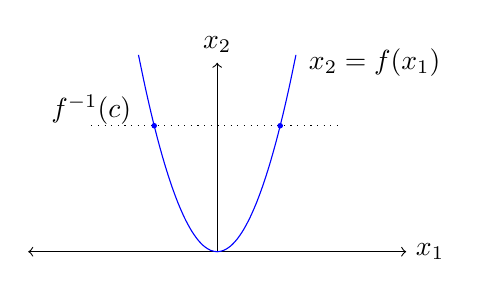
\begin{tikzpicture}[scale=0.8]
		\draw[<->] (-3, 0) -- (3, 0) node[right] {$x_1$};
  		\draw[->] (0, 0) -- (0, 3) node[above] {$x_2$};
  		\draw[scale=0.5, domain=-2.5:2.5, smooth, variable=\x, blue] plot ({\x}, {\x*\x});
		\draw[dotted,thin,black] (-2,2) -- (2,2);
		\draw (-2,2.25) node{$f^{-1}(c)$};
		\draw (2.5,3) node{$x_2 = f(x_1)$};
		\node[circle,fill=blue,inner sep=0pt, minimum size=2pt] at (1,2){};
		\node[circle,fill=blue,inner sep=0pt, minimum size=2pt] at (-1,2){};
\end{tikzpicture}
	\caption{Graph of $f(x_1)=x_1^2$ and Level set $f^{-1}(c)$}
\end{figure}

%\chapter{Vector Fields}
\section{Vector Fields}
\begin{definition}
	A vector $\mathbf{v}$ at a point $p \in \mathbb{R}^{n+1}$ is a pair $\mathbf{v} = (p,v)$ where $v \in \mathbb{R}^{n+1}$.
\end{definition}
\begin{description}
	\item[vector addition] $\mathbf{v} + \mathbf{w} = (p,v) + (p,w) = (p,v+w)$.
	\item[scalar multiplication] Let $c \in \mathbb{R}$, then $c \mathbf{v} =  c(p,v) = (p,cv)$.
	\item[dot product] $\mathbf{v}\cdot \mathbf{w} = (p,v)\cdot(p,w) = v \cdot w$
	\item[cross product] $\mathbf{v}\times \mathbf{w} = (p,v)\times(p,w) = (p,v \times w)$
\end{description}
\begin{remark}
	Angle $\theta$ between $\mathbf{v}$ and $\mathbf{w}$ is given by,
	\begin{equation}
		\cos \theta = \mathbf{v}\cdot\mathbf{w} = (p,v)\cdot(p,w) = v.w
	\end{equation}
	And the length of a vector $\mathbf{v}$ is given by,
	\begin{equation}
		\|\mathbf{v}\| = \mathbf{v}\cdot\mathbf{v} = (p,v)\cdot(p,v) = v\cdot v = \| v \|
	\end{equation}
\end{remark}

\begin{remark}
	Let $c \in \mathbb{R}$ and $p \in \mathbb{R}^{n+1}$. Let $\mathbf{v}, \mathbf{w}$ be two vectors at $p$. That is, $\mathbf{v} = (p,v)$ and $\mathbf{w} = (p,w)$ for some $v,w \in \mathbb{R}^{n+1}$. Then the set of all vectors at $p$ is a vector space with vector addition $\mathbf{v}+\mathbf{w} = (p,v+w)$ and scalar multiplication $c\mathbf{v} = (p,cv)$. This vector space is denoted by $\mathbb{R}_p^{n+1}$.
\end{remark}

\begin{figure}[h]
	\centering
	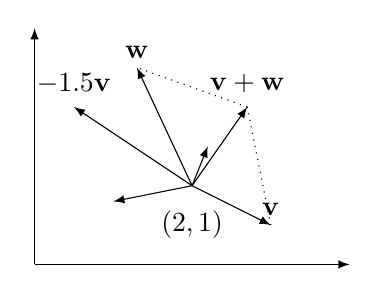
\begin{tikzpicture}
		\draw[-latex] (0,0) -- (0,3);
		\draw[-latex] (0,0) -- (4,0);

		\draw[-latex] (2,1) -- (1,0.8);
		\draw[-latex] (2,1) -- (2.2,1.5);
		%\draw[-latex] (2,1) -- (3,1.25);
		\draw[-latex] (2,1) -- (1.3,2.5); %w
		\draw[-latex] (2,1) -- (3,0.5); %v
		\draw[-latex] (2,1) -- (2.7,2); %v+w
		\draw[-latex] (2,1) -- (0.5,2); %1.5v
		\draw[dotted,thin] (3,0.5) -- (2.7,2);
		\draw[dotted,thin] (2.7,2)-- (1.3,2.5);

		\draw (2,0.5) node{$(2,1)$};
		\draw (3,0.7) node{$\mathbf{v}$};
		\draw (1.3,2.7) node{$\mathbf{w}$};
		\draw (2.7,2.3) node{$\mathbf{v+w}$};
		\draw (0.5,2.3) node{$-1.5\mathbf{v}$};
	\end{tikzpicture}
	\caption{The vector space of all vectors at $(2,1)$, $\mathbb{R}_{(2,1)}^2$}
\end{figure}

\begin{definition}
	The vector field $\mathbf{X}$ on $\mathbb{R}^{n+1}$ is a function which assigns to each point of $\mathbb{R}^{n+1}$ a vector at that point.
	That is, $\mathbf{X}(p) = (p,X(p))$.
\end{definition}

For example, $\mathbf{X}(p) = (p,X(p))$ where the associated function of the vector field, $X : \mathbb{R}^2 \to \mathbb{R}^2$ defined by $X(p) = (1,2)$ assigns a constant vector $(1,2)$ at every vector in $\mathbb{R}^2$.

\begin{figure}[h]
	\centering
	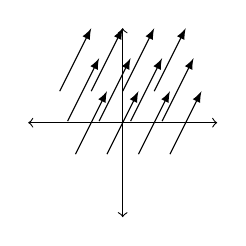
\begin{tikzpicture}[scale=0.4]
		\draw[<->] (-3,0) -- (3,0);
		\draw[<->] (0,-3) -- (0,3);

		\draw[-latex] (1,1) -- (2,3);
		\draw[-latex] (0,1) -- (1,3);
		\draw[-latex] (-1,1) -- (0,3);
		\draw[-latex] (-2,1) -- (-1,3);

		\draw[-latex] (1.25,0.05) -- (2.25,2.05);
		\draw[-latex] (0.25,0.05) -- (1.25,2.05);
		\draw[-latex] (-0.75,0.05) -- (0.25,2.05);
		\draw[-latex] (-1.75,0.05) -- (-0.75,2.05);

		\draw[-latex] (1.5,-1) -- (2.5,1);
		\draw[-latex] (0.5,-1) -- (1.5,1);
		\draw[-latex] (-0.5,-1) -- (0.5,1);
		\draw[-latex] (-1.5,-1) -- (-0.5,1);

	\end{tikzpicture}
	\caption{Vector field with associated function $X(p) = (1,2)$}
\end{figure}

\begin{definition}[smooth]
	A function $f : \mathbb{R} \to \mathbb{R}$ is smooth if its partial derivatives of all orders exists and are continuous.
	A function $f : \mathbb{R}^{n+1} \to \mathbb{R}$ is smooth if its component functions $f = (f_1, f_2, \cdots, f_{n+1})$ are smooth.
	A vector field $\mathbf{X}$ is smooth if the associated function $X(p)$ is smooth.
\end{definition}

\begin{definition}
	Let $f : \mathbb{R}^{n+1} \to \mathbb{R}$. Then the gradient of $f$ at $p$ is,
	\begin{equation}
		\nabla f(p) = \left(p,\frac{\partial f}{\partial x_1}(p),\frac{\partial f}{\partial x_2}(p),\cdots,\frac{\partial f}{\partial x_{n+1}}(p)\right)
	\end{equation}
\end{definition}

\begin{remark}
	If $f$ is a smooth function, then the gradient of $f$ at $p$ is a smooth vector field.
\end{remark}
	For example, $f : \mathbb{R}^2 \to \mathbb{R}$ defined by $f(x_1,x_2) = 2x_1x_2$ is a smooth function. We have, $\frac{\partial f}{\partial x_1} = 2x_2$ and $\frac{\partial f}{\partial x_2} = 2x_1$. And gradient of $f$ at $(x_1,x_2)$ is $(x_1,x_2,2x_2,2x_1)$. That is, $(2x_2,2x_1)$ at $(x_1,x_2)$.

Calculations : \\
\begin{tabular}{|c|c|c|c|c|c|c|} \hline
	$p$    & $(x_1,x_2)$   & $(0,0)$ & $(1,0)$ & $(0,1)$ & $(-1,0)$ & $(0,-1)$ \\ \hline
	$X(p)$ & $(2x_2,2x_1)$ & $(0,0)$ & $(0,2)$ & $(2,0)$ & $(0,-2)$ & $(-2,0)$ \\ \hline
\end{tabular}

\begin{figure}[h]
	\centering
	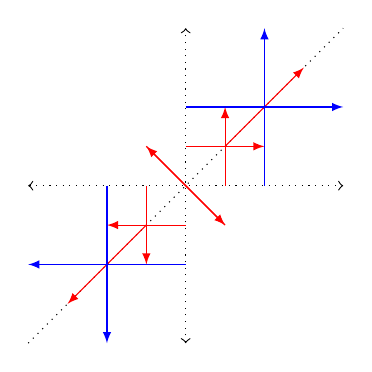
\begin{tikzpicture}[scale=0.5]
		\draw[<->,dotted] (0,-4) -- (0,4);
		\draw[<->,dotted] (-4,0) -- (4,0);
		\draw[dotted] (-4,-4) -- (4,4);

		\draw[-latex,color=red] (1,1) -- (3,3);
		\draw[-latex,color=red] (-1,1) -- (1,-1);
		\draw[-latex,color=red] (1,-1) -- (-1,1);
		\draw[-latex,color=red] (-1,-1) -- (-3,-3);
		\draw[-latex,color=red] (0,1) -- (2,1);
		\draw[-latex,color=red] (0,-1) -- (-2,-1);
		\draw[-latex,color=red] (1,0) -- (1,2);
		\draw[-latex,color=red] (-1,0) -- (-1,-2);

		%\draw[-latex] (-1,2) -- (3,0);
		%\draw[-latex] (2,-1) -- (0,3);
		%\draw[-latex] (1,-2) -- (-3,0);
		%\draw[-latex] (-2,1) -- (0,-3);

		\draw[-latex,color=blue] (0,2) -- (4,2);
		\draw[-latex,color=blue] (2,0) -- (2,4);
		\draw[-latex,color=blue] (-2,0) -- (-2,-4);
		\draw[-latex,color=blue] (0,-2) -- (-4,-2);

		%\draw[-latex] (1,0.5) -- (2,2.5);
		%\draw[-latex] (0.5,1) -- (2.5,2);
		%\draw[-latex] (-1,0.5) -- (0,-1.5);
		%\draw[-latex] (0.5,-1) -- (-1.5,0);
		%\draw[-latex] (1,-0.5) -- (0,1.5);
		%\draw[-latex] (-0.5,1) -- (1.5,0);
		%\draw[-latex] (-1,-0.5) -- (-2,-2.5);
		%\draw[-latex] (-0.5,-1) -- (-2.5,-2);
	\end{tikzpicture}
	\caption{The gradient of $f(x_1,x_2) = 2x_1x_2$}
\end{figure}

\begin{definition}
	A parameterised curve is a function, $\alpha : I \to \mathbb{R}^{n+1}$ where $I$ is some open interval in $\mathbb{R}$.
	The velocity vector of a parameterised curve $\alpha : I \to \mathbb{R}^{n+1}$ at a point $\alpha(t)$ is the tangent to the curve at that point.
	\begin{equation}
		\dot{\mathbf{\alpha}}(t) = \left(\alpha(t),\frac{d \alpha}{dt} (t)\right)
	\end{equation}
\end{definition}

For example, $\alpha : I \to \mathbb{R}^2$ defined by $\alpha(t) = (2t,t^2)$ is a parameterised curve. We have, $\frac{d\alpha}{dt} = (\frac{dx_1}{dt}(t),\frac{dx_2}{dt}(t)) = (2,2t)$ where $\alpha(t) = (x_1(t),x_2(t))$. The velocity vector at $t = 3$ is $\dot{\alpha}(3) = (\alpha(t),\frac{d\alpha}{dt}) = (6,9,2,6)$.

\begin{definition}
	Let $\mathbf{X}$ be a vector field and let $U$ be an open subet of $\mathbb{R}^{n+1}$.
	An integral curve $\alpha$ on $U$ is a parameterised curve, $\alpha : I \to \mathbb{R}^{n+1}$ such that for each $\alpha(t) = p \in U$, the velocity vector $\dot{\alpha}(t)$ is the associated vector $\mathbf{X}(p)$ of the vector field $\mathbf{X}$ at that point. Thus, for each $t \in I$, $\dot{\alpha}(t) = \mathbf{X}(\alpha(t))$.
	\begin{equation}
		\left(\alpha(t),\frac{d \alpha}{dt}(t)\right) = \left(\alpha(t),X(\alpha(t))\right)
	\end{equation}
	Let $X(p) = \left(X_1(p),X_2(p),\cdots,X_{n+1}(p)\right)$ and $\alpha(t) = \left(x_1(t),x_2(t),\cdots,x_{n+1}(t)\right)$. Then, comparing components of the vector at $\alpha(t)$ we get the following system of equations,
	\begin{equation}
		\frac{d x_j}{dt}(t) = X_j(\alpha(t)),\ j = 1,2,\cdots,(n+1)
	\end{equation}
\end{definition}

For example, Consider $\alpha : (2,3) \to \mathbb{R}^2$ defined by $\alpha(t) = (t,t^2)$. Then $\alpha$ is a parameterised curve in vector field, $\mathbf{X}$ which has the associated function $X(x_1,x_2) = (1,2x_1)$. Then, $\mathbf{X}(x_1,x_2) = (x_1,x_2,1,2x_1)$. And
\[ \dot{\alpha}(t) = \left( \alpha(t),\frac{d\alpha}{dt}(t) \right) = \left( x_1(t),x_2(t),\frac{dx_1}{dt}(t), \frac{dx_2}{dt}(t) \right) = (t,t^2,1,2t) \]
Clearly, $\alpha$ is an integral curve of $\mathbf{X}$ as $\dot{\alpha}(t) = X(\alpha(t))$ for every $t \in (2,3)$.

Calculations:\\
\begin{tabular}{|c|c|c|c|c|c|c|c|c|c|} \hline
	$p$    & $(0,0)$ & $(1,0)$ & $(0,1)$ & $(1,1)$ & $(-1,0)$ & $(0,-1)$ & $(-1,1)$ & $(1,-1)$ & $(-1,-1)$ \\ \hline
	$X(p)$ & $(1,0)$ & $(2,2)$ & $(1,1)$ & $(2,3)$ & $(0,-2)$ & $(1, 1)$ & $(0,-1)$ & $(2, 1)$ & $( 0,-3)$ \\ \hline
\end{tabular}

\begin{figure}[h]
	\centering
	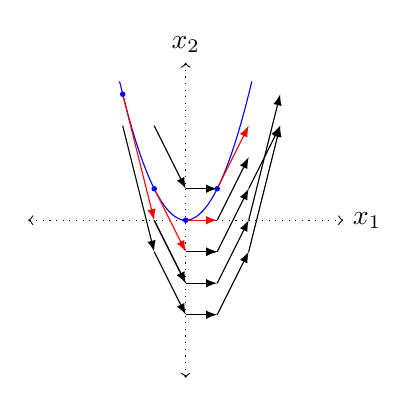
\begin{tikzpicture}[scale=0.4]
		\draw[<->,dotted] (-5, 0) -- (5, 0) node[right] {$x_1$};
  		\draw[<->,dotted] (0,-5) -- (0, 5) node[above] {$x_2$};
  		\draw[domain=-2.1:2.1, smooth, variable=\x, blue] plot ({\x}, {\x*\x});

		\draw[-latex,color=red] (0,0) -- (1,0);

		\draw[-latex] (0,1) -- (1,1);
		\draw[-latex] (1,0) -- (2,2);
		\draw[-latex] (-1,3) -- (0,1);

		\draw[-latex,color=red] (-2,4) -- (-1,0);
		\draw[-latex,color=red] (1,1) -- (2,3);

		\draw[-latex] (0,-1) -- (1,-1);
		\draw[-latex,color=red] (-1,1) -- (0,-1);

		\draw[-latex] (-1,0) -- (0,-2);
		\draw[-latex] (0,-2) -- (1,-2);
		\draw[-latex] (1,-2) -- (2,0);
		\draw[-latex] (2,0) -- (3,4);

		\draw[-latex] (0,-1) -- (1,-1);
		\draw[-latex] (-1,0) -- (0,-2);

		\draw[-latex] (-2,3) -- (-1,-1);
		\draw[-latex] (-1,-1) -- (0,-3);
		\draw[-latex] (0,-3) -- (1,-3);
		\draw[-latex] (1,-3) -- (2,-1);
		\draw[-latex] (2,-1) -- (3,3);

		\draw[-latex] (0,-1) -- (1,-1);
		\draw[-latex] (1,-1) -- (2,1);
		\draw[-latex] (2,1) -- (3,3);

		\node[circle,fill=blue,inner sep=0pt, minimum size=2pt] at (1,1){};
		\node[circle,fill=blue,inner sep=0pt, minimum size=2pt] at (0,0){};
		\node[circle,fill=blue,inner sep=0pt, minimum size=2pt] at (-1,1){};
		\node[circle,fill=blue,inner sep=0pt, minimum size=2pt] at (-2,4){};
\end{tikzpicture}
	\caption{Integral Curve $\alpha(t) = (t,t^2)$ in $\mathbf{X}$ with $X(x_1,x_2) = (1,2x_1)$}
\end{figure}

\begin{theorem}
	Let $\mathbf{X}$ be a smooth vector field on an open set $U \subset \mathbb{R}^{n+1}$ and let $p \in U$.
	Then there exists an open interval $I$ containing $0$ and an integral curve $\alpha : I \to U$ such that
	\begin{enumerate}
		\item $\alpha(0) = p$
		\item If $\beta : \tilde{I} \to U$ is any other integral curve with $\beta(0) = p$, then $\tilde{I} \subset I$ and $\beta(t) = \alpha(t)$, for all $t \in \tilde{I}$.
	\end{enumerate}
\end{theorem}
\begin{proof}
	Let $\mathbf{X}$ be a smooth vector field.
	Suppose $\alpha$ be an integral curve in $\mathbf{X}$.
	Then, $\dot{\alpha}(t) = \mathbf{X}(\alpha(t))$.
	Let $x_j(t)$ be the components of $\alpha(t)$ and $X_j(p)$ be the components of $X(p)$.
	\begin{align*}
		\dot{\alpha}(t) & = \left(\alpha(t),\frac{d \alpha}{dt}(t)\right) \\
		& = \left(x_1(t),\cdots,x_{n+1}(t),\frac{dx_1}{dt}(t),\cdots,\frac{dx_{n+1}}{dt}(t)\right)\\
		\mathbf{X}(\alpha(t)) & = (\alpha(t),X(\alpha(t))) \\
		& = \left( x_1(t),\cdots,x_{n+1}(t),X_1(\alpha(t)),\cdots,X_{n+1}(\alpha(t))\right)
	\end{align*}
	Thus, we a system of $n+1$ first order differential equations in $n+1$ unknowns satisfying the initial condition $\alpha(0) = p$.
	\begin{align*}
		\frac{dx_1}{dt}(t) & = X_1(\alpha(t)) \\
		\frac{dx_2}{dt}(t) & = X_2(\alpha(t)) \\
		& \vdots \\
		\frac{dx_{n+1}}{dt}(t) & = X_{n+1}(\alpha(t))
	\end{align*}
\end{proof}
	By the theorem on solution of systems of first order ordinary differential equations, there exists an interval $I$ containing $0$ and a solution --- a family of functions $\{ x_1(t), x_2(t), \cdots,x_{n+1}(t)\}$ satisfying the above system of equations satisfying the initial condition $\alpha(0) = p$.

	Define $\alpha : I \to U$ using the component functions of $\alpha$ as $x_j$s in the above solution. Then, we have a integral curve of the vector field $\mathbf{X}$ satifying the initial condition $\alpha(0) = p$.

	Let $\beta : \tilde{I} \to U$ be another integral curve with $\beta(0) = p$. Then by the uniqueness of the solution for the system of first order ordinary differential equations with an initial condition, $\beta(t) = \alpha(t)$ for every $ t \in I \cup \tilde{I}$.

	Let $\{\beta_1,\beta_2,\cdots\}$ be the family of integral curves with $\beta_j : I_j \to U$ satisfying $\beta_j(0) = p$. Consider $I = \bigcup\limits_{j \in \mathbb{N}} I_j$.

	Define $\alpha : I \to U$ by $\alpha(t) = \beta_j(t)$ where $t \in I_j$ for some $j \in \mathbb{N}$. Then $\alpha$ is well-defined and is a maximal integral curve in $\mathbf{X}$ such that $\alpha(0) = p$.

\begin{definition}
	A smooth vector field $\mathbf{X}$ on $U \subset \mathbb{R}^{n+1}$ is \textbf{complete} if for every $p \in U$, the maximal integral curve through $p$ has domain equal to $\mathbb{R}$.
\end{definition}

\begin{definition}
	The \textbf{divergence} of a smooth vector field $\mathbf{X}$ on $U \subset \mathbb{R}^{n+1}$ is the function $div\ \mathbf{X} : U \to \mathbb{R}$ defined by
	\[ div\ X(x_1,x_2,\cdots,x_{n+1}) = \sum_{i=1}^{n+1} \frac{\partial X_i}{\partial x_i} \]
	where $X_i$ are the component function of the associated function $X$ of the vector field $\mathbf{X}$.
\end{definition}

For example, Consider $\mathbf{X}$ with associated function $X : \mathbb{R}^2 \to \mathbb{R}^2$ defined by $X(x_1,x_2) = (2x_1,x_1x_2)$. Then $div\ \mathbf{X}(x_1,x_2) = \frac{\partial X_1}{\partial x_1} + \frac{\partial X_2}{\partial x_2} = 2 + x_1$.

%\chapter{The Tangent Space}
\section{The Tangent Space}

%\chapter{Surfaces}
\section{Surfaces}

%\chapter{Vector Fields on Surfaces; Orientation}
\section{Vector Fields on Surfaces; Orientation}

%\chapter{The Gauss Map}
\section{The Gauss Map}
	Suppose $S$ is an $n$-surface. From the definition of an $n$-surface, there exists a smooth function $f : U \to \mathbb{R}$ where $U$ is an open subset of $\mathbb{R}^{n+1}$ such that $S = f^{-1}(c)$ for some real value $c \in \mathbb{R}$ and every point on $S$ is a regular point of $f$. That is $\nabla f(p) \ne \mathbf{0}$ for every point $p$ on the surface $S$.\\

	We have proved that every $n$-surface has exactly two orientations $\mathbf{N}_1$ and $\mathbf{N}_2$. These orientations are $\frac{\nabla f}{\| \nabla f\|}$ and $\frac{-\nabla f}{\| \nabla f\|}$. Given an orientation $\mathbf{N}$ (either $\mathbf{N}_1$ or $\mathbf{N}_2$), the surface together with that orientation is collectively referred as an oriented $n$-surface.\\

	\textbf{Since orientation $\mathbf{N}$ is a smooth, unit normal vector field. The vector field $\mathbf{N}$ has an associated function $N : U \to \mathbb{R}^{n+1}$. That is $\mathbf{N}(p) = (p,N(p))$ where $N : U \to \mathbb{R}^{n+1}$. And we already have, $\mathbf{N}(p) = (p,N(p)) = (p, \frac{\pm \nabla f}{\| \nabla f\|})$. This associated function restricted to the $n$-surface $S$ is the \textbf{Gauss Map}. That is, $N : S \to \mathbb{R}^{n+1}$.}\\

	From the definition of orientation, we know that this function is actually assigning direction to each point on that surface $S$. If you don't remember, the directions are vector in $\mathbb{R}^{n+1}$ of unit length. That is $\|v\| = 1$. Thus, the range of Gauss Map is a subset of the set of all directions. And unit sphere $S^n$ is $\mathbb{R}^{n+1}$ is the set of all directions in $\mathbb{R}^{n+1}$.\\

	Thus, we may write Gauss Map, $N : S \to S^n$
\subsection{Spherical Image}
	We already saw that, the Gauss Map $N : S \to S^n$ is a function which maps directions/unit vectors to each point on that oriented surface $S$.\\

	Do we need an oriented surface ? Yes. The Gauss Map is defined by this orientation. If we are provided with an oriented $n$ Surface $S$, then we have a unit vector/orientation assigned to each point $p$ on that surface. And Gauss Map assigns this unit vector to the point $p$ on surface $S$.\\

	We already saw that the range of the Gauss Map is a subset of the unit $n$ Sphere $S^n$. In other words, the Gauss Map assigns each point on the oriented $n$-surface $S$ into a subset of the unit $n$ sphere $S^n$. Thus, \textbf{range of the Gauss Map is referred as the spherical image of the oriented $n$-surface $S$}.
	\begin{equation}
	N(S) = \{ q \in S^n : q = N(p),\ p \in S \}
	\end{equation}

\subsection{Compact, connected, oriented $n$ Surface}
	Suppose we have a compact, connected, oriented $n$-surface $S$. The compact subsets in Euclidean spaces are closed and bounded subsets. And connected subsets in Euclidean Spaces are path connected.\\

\begin{theorem}[Spherical Image of Compact, Connected, Oriented Surface]
	The Gauss map of a compact, connected, oriented $n$-surface is surjective.
\end{theorem}
\begin{proof}
	Let $v \in S^n$ be a direction in $\mathbb{R}^{n+1}$. Let $S$ be a compact, connected, oriented $n$-surface with orientation $N$ such that $S = f^{-1}(c)$ and every point $p \in S$ are regulr points of the smooth function $f : U \to \mathbb{R}$ where $U$ is an open subset of $\mathbb{R}^{n+1}$. Thus, we have the Gauss Map $N: S \to S^n$ defined by the orientation on $S$.\\
	
	Since $v$ is arbitary, it is enough to prove that $v \in N(S)$. Suppose there exists $v \in S^n$ such that $v \notin N(S)$, then the Gauss Map is not surjective. In other words, $N$ is surjective if for every $v \in S^n,\ v \in N(S)$ OR for every $v \in S^n$, there exists $p \in S$ such that $v = N(p)$\\

	Let $g : \mathbb{R}^{n+1} \to \mathbb{R}$ defined by $g(p) = p \cdot v$. Then $g$ is a smooth function since first order partial derivatives are constant functions and all other partial derivatives of higher orders vanishes.\\

	Since $S$ is compact, $g$ restricted to $S$ is a continuous function defined on a compact interval. And thus it attains maximum and minimum values, say $p$ and $q$. The maximum and minimum values of the dot product $p \cdot v$ are $\pm v$.\\
	
	By Lagrange's multiplier theorem, $\nabla g(p) = \lambda \nabla f(p)$ and $\nabla g(q) = \lambda \nabla f(q)$. From the definition of the Gauss Map, we have $\nabla g(p) = \lambda \nabla f(p) = \lambda \| \nabla f(p) \| \mathbf{N}(p) = \lambda \| \nabla f(p) \| (p,v)$. Thus, $v$ and $N(p)$ are multiples of one another. Similarly, $\nabla g(q) = \lambda \| \nabla f(q) \| \mathbf{N}(q)$. Therefore $N(p) = \pm v$ and $N(q) = \pm v$.\\
	
	It remains to show that $N(p) \ne N(q)$. Suppose $N(p) = N(q)$. If there exists continuous function $\alpha$ such that $\alpha : [0,1] \to \mathbb{R}^{n+1}$, $\alpha(0) = p$, $\alpha(1) = q$, $\dot{\alpha}(0) = (p,v)$ and $\dot{\alpha}(1) = (q,v)$. And $\alpha$ maps the interior, the open interval $(0,1)$ outside the surface $S$. Then by intermediate value theorem, we arrive at a contradiction. And thus $N(p) \ne N(q)$.\\

	Let $\alpha_1 : [0,x] \to \mathbb{R}^{n+1}$ defined by $\alpha_1(t) = p+tv$. Let $\alpha_2 : [y,1] \to \mathbb{R}^{n+1}$ defined by $\alpha_2(t) = q+(t-1)v$. Let $\alpha_3 : [x,y] \to S_1$ where $S_1$ is an $n$ sphere properly containing $S$. Such an $n$ sphere exists, since $S$ is compact (bounded). And there exists such a function $\alpha_3$, the image of which is a compact subset of $S_1$.\\
	
	Now consider $\alpha : [0,1] \to \mathbb{R}^{n+1}$ defined by
	\begin{equation}
		\alpha(t) = \begin{cases} \alpha_1(t) & t \in [0,x) \\ \alpha_3(t) & t \in [x,y] \\ \alpha_2(t) & t \in (y,1] \end{cases}
	\end{equation}

\begin{figure}[hbt]
	\centering
	\begin{tikzpicture}[scale=0.6]

	\draw (2,2.5) node{$p$};
	\draw (-0.5,-1.55) node{$q$};
	\draw plot [smooth cycle, tension=1] coordinates {(1,1) (2,3) (4,0) (2,-0.5) (0,-2) (-2,-1)};

	\draw (0,0.7) node{$S$};
	\draw (0,5.5) node{$S_1$};
	\draw[thick,blue] (1.8,3.05) -- (1.8,4.85);
	\draw (2.5,3.8) node{$\alpha_1$};

	\draw[thick,brown] (-0.5,-2.05) -- (-0.5,-3.9);
	\draw (0,-2.7) node{$\alpha_2$};

	\draw (-4,2.5) node{$\alpha_3$};
	\begin{scope}
		\clip (1.8,0) rectangle (-6,6);
		\draw[thick,color=red] (0.5,0.5) circle (4.5cm);
	\end{scope}
	\begin{scope}
		\clip (-0.5,-5) rectangle (-6,0);
		\draw[thick,color=red] (0.5,0.5) circle (4.5cm);
	\end{scope}
\end{tikzpicture}
	\caption{Construction of $\alpha$}
\end{figure}

	Clearly, $\alpha$ is a smooth function with $\alpha(t) \notin S,\ t \in (0,1)$ and 
	\begin{align*}
		\alpha(0) & = \alpha_1(0) = p+0v = p \\
		\alpha(1) & = \alpha_2(1) = q + (1-1)v = q\\
		\dot{\alpha}(0) & = \dfrac{d\alpha_1}{dt}(0) = \dfrac{d (p+tv)}{dt}(0) = v\\
		\dot{\alpha}(1) & = \dfrac{d\alpha_2}{dt}(1) = \dfrac{d (q+(t-1)v}{dt} = v
	\end{align*}

	We have, $f(\alpha(0)) = f(0) = c$ since $p \in S = f^{-1}(c)$. Similarly, $f(\alpha(1)) = c$. And $(f \circ \alpha)'(0) = \nabla f \circ \alpha(0) \dot \dot{\alpha}(0) = \nabla f(p) \cdot \dot{\alpha}(0) = \| \nabla f(p) \| N(p) \cdot v$. Similarly, $(f \circ \alpha)'(1) = \| \nabla f(q) \| N(q) \cdot v$. We have assumed that $N(p) = N(q)$. Then, $f \circ \alpha$ is either increasing at both $0$ and $1$ OR decreasing at both $0$ and $1$.\\

	Without Loss of Generality, Suppose that $f \circ \alpha$ is increasing at either points. Then, there exists a sufficiently small $\epsilon > 0$ such that $f(\alpha(\epsilon)) > c$ and $f(\alpha(1-\epsilon)) < c$. Since, $f \circ \alpha$ must have a value greater than $c$ immediately after $0$ and should have a value less than $c$ just before reaching $1$ as the function is increasing at either points (and in some small neighbourhood of those points).\\

	By Intermediate Value theorem, the exists $t \in (0,1)$ such that $f \circ \alpha(t) = c$ since the composition of smooth functions $f$ and $\alpha$ is also smooth. But, it is clear from the construction that $\alpha(t)$ doesn't belong to the surface $S$. And therefore, $\alpha(t) \ne c \implies f(\alpha(t)) \ne c$ for any $t \in (0,1)$. Thus by contradiction, $N(p) \ne N(q)$. And if $N$ achieves $v$ at $p$. Then it achieves $-v$ at $q$. And since $v \in S^n$ is arbitrary, $N(S) = S^n$ and the spherical image is the entire $n$ sphere OR the Gauss map is surjective.
\end{proof}

	\textbf{Given a compact, connected oriented, $n$-surface $S$, the Gauss Map on $S$ is surjective. In other words, the spherical image of such a surface is the unit $n$ sphere $S^n$ itself.}\\

	Connectedness is not that critical(in my opinion). For a compact, orientated $n$-surface with multiple components, the above observation is valid for each connected component. And thus for any compact, oriented surface. Again, $n$-surfaces are always closed. Thus, the restriction practically reduces to boundedness of the $n$-surface.

%\chapter{Geodesics}
\section{Geodesics}
	We already know that our earth is not flat. Still, we feel like we move in straight lines. And our `straight lines' are curved for an observer who is not on earth. Geodesics are straightlines on an $n$-surface $S$.

\begin{description}
	\item[vector field along $\alpha$] is function which assigns $X(t)$ at $\alpha(t)$ for each $t \in I$.
		The defintion of vector field doesn't allow you to assign multiple vectors at a point. But, vector field along $\alpha$ allows you to assign vectors to points on a parametrised curve depending on the value of parameter $t$.
	\item[function along $\alpha$] is function with the same domain $I$ as $\alpha$.
	\item[derivative of vector field $\mathbf{X}$ along $\alpha$] is a vector field along $\alpha$ given by $\dot{\mathbf{X}}(t) = \left( \alpha(t), \dfrac{dX}{dt}(t) \right)$ where $\mathbf{X}(t) = \left( \alpha(t), X(t) \right)$.
	\item[velocity of $\alpha$] is a vector field along $\alpha$ defined by $\dot{\boldsymbol{\alpha}}(t)= \left( \alpha(t), \dfrac{d\alpha}{dt}(t) \right)$.\\
		Suppose $\alpha : I \to \mathbb{R}^2$ is defined by $\alpha(t) = (3t,t^2)$.\\
		Then velocity of $\alpha$ is $\dot{\boldsymbol{\alpha}}(t) = \left( \alpha(t),\dfrac{d\alpha}{dt}(t) \right) = (3t,t^2,3,2t)$.
	\item[speed of $\alpha$] is $\| \dot{\boldsymbol{\alpha}}(t) \|$.\\
		Speed of $\alpha$ is $\| \dot{\boldsymbol{\alpha}}(t) \| = \sqrt{9+4t^2}$.
	\item[acceleration $\alpha$] is a vector field along $\alpha$ defined by $\ddot{\boldsymbol{\alpha}}(t) = \left( \alpha(t), \dfrac{d^2\alpha}{dt^2}(t) \right)$.\\
		Acceleration of $\alpha$ is $\ddot{\boldsymbol{\alpha}}(t) = (3t,t^2,0,2)$
\end{description}

\subsection{Properties of differentiation}
Let $\mathbf{X},\mathbf{Y}$ be smooth vector fields along parametrised curve $\alpha : I \to \mathbb{R}^{n+1}$.
\begin{itemize}
	\item $\dot{(\mathbf{X}+\mathbf{Y})} = \dot{\mathbf{X}} + \dot{\mathbf{Y}}$
	\begin{align*}
		(\mathbf{X}+\mathbf{Y})(t) = & (\alpha(t), X(t)) + (\alpha(t), Y(t)) = \left( \alpha(t), X(t)+Y(t) \right) \\
		\dot{(\mathbf{X}+\mathbf{Y})}(t) = & \left( \alpha(t), \dfrac{d}{dt} X(t)+Y(t) \right) \\
		= & \left( \alpha(t), \dfrac{d}{dt}X(t)\right) + \left( \alpha(t), \dfrac{d}{dt}Y(t) \right) \\
		= & \dot{\mathbf{X}}(t) + \dot{\mathbf{Y}}(t)
	\end{align*}
	\item $\dot{(f\mathbf{X})} = f'\mathbf{X} + f\dot{\mathbf{X}}$
	\begin{align*}
		f\mathbf{X}(t) = & f(t)(\alpha(t), X(t)) = (\alpha(t), f(t)X(t)) \\
		\dot{(f\mathbf{X})}(t) = & \left( \alpha(t),\dfrac{d}{dt}f(t)X(t) \right) \\
		= & \left( \alpha(t), f'(t)X(t) + f(t)\dfrac{dX}{dt}(t) \right) \\
		= & \left( \alpha(t), f'(t)X(t) \right) + \left( \alpha(t), f(t)\dfrac{d}{dt} \mathbf{X}(t) \right)\\
		= & f'(t) \left( \alpha(t),X(t) \right) + f(t) \left( \alpha(t),\dfrac{d}{dt} X(t) \right)\\
		= & f'\mathbf{X}(t) + f\dot{\mathbf{X}}(t)
	\end{align*}
	\item $(\mathbf{X} \cdot \mathbf{Y})' = \dot{\mathbf{X}} \cdot \mathbf{Y} + \mathbf{X} \cdot \dot{\mathbf{Y}}$
	\begin{align*}
		(\mathbf{X} \cdot \mathbf{Y}) = & (\alpha(t), X(t)) \cdot (\alpha(t),Y(t)) = \sum_{k = 1}^{n+1} X_k(t)Y_k(t) \\
		(\mathbf{X} \cdot \mathbf{Y})' = & \dfrac{d}{dt} \sum_{k = 1}^{n+1} X_k(t)Y_k(t) \\
		= & \sum_{k = 1}^{n+1} \dfrac{d}{dt}X_k(t)Y_k(t)\\
		= & \sum_{k = 1}^{n+1} X_k'(t)Y_k(t) + X_k(t)Y_k'(t)
	\end{align*}
	$$\dot{\mathbf{X}}(t) \cdot \mathbf{Y}(t) =  \left( \alpha(t), \dfrac{d}{dt}X(t) \right) \cdot \left( \alpha(t), Y(t) \right) =  \sum_{k=1}^{n+1} X_k'(t)Y_k(t)$$
		$$\mathbf{X}(t) \cdot \dot{\mathbf{Y}}(t) =  \left( \alpha(t), X(t) \right) \cdot \left( \alpha(t), \dfrac{d}{dt}Y(t) \right) =  \sum_{k=1}^{n+1} X_k(t)Y_k'(t)$$
\end{itemize}

\begin{definition}[geodesic]
	Let $S$ be an $n$-surface. A Geodesic on $S$ is a parametrised curve $\alpha : I \to S$ whose acceleration is orthogonal to $S$ everywhere.
\end{definition}

%\chapter{Parallel Transport}
\section{Parallel Transport}

%\chapter{The Weingarten Map}
\section{The Weingarten Map}

%\chapter{The Curvature of Plane Curves}
\section{The Curvature of Plane Curves}

%\chapter{Arc Length and Line Integrals}
\section{Arc Length and Line Integrals}

%\chapter{Curvature of Surfaces}
\section{Curvature of Surfaces}

%\chapter{Convex Surfaces}
\setcounter{section}{13}
%\chapter{Parameterized Surfaces}
\section{Parameterized Surfaces}

%\chapter{Local Equivalence of Surfaces and Parameterized Surfaces}
%\chapter{Focal Points}
%\chapter{Surface Area and Volume}
%\chapter{Minimal Surfaces}
%\chapter{The Exponential Map}
%\chapter{Surfaces with Boundary}
%\chapter{The Gauss-Bonnet Theorem}
%\chapter{Rigid Motions and Congruence}
%\chapter{Isometries}
%\chapter{Riemannian Metrics}

\chapter{ME800402 Algorithmic Graph Theory}
%Text Books : \cite{chartrand}
%Module 1 : Introduction to Graphs and Algorithms
%What is graph? The degree of a vertex, isomorphic graphs, subgraphs, degree sequences, connected graphs, cutvertices and blocks, special graphs, digraphs, algorithmic complexity, Search algorithms, sorting algorithms, greedy algorithms,, representing graphs in a computer.
%( Chapter 1 Sections 1.1 to 1.9, Chapter 2 Sections 2.1, 2.2 , 2.3, 2.5 and 2.6 of \cite{chartrand} ) (24 hours)
%Module 2 : Trees, paths and distances
%Properties of trees, rooted trees, Depth-first search, breadth-first search, the minimum spanning tree problem
%Distance in a graphs, distance in weighted graphs, the centre and median of a graph, Activity digraphs and critical paths.
%(Chapter 3 sections 3.1 to 3.3, 3.4 and 3.5 , Chapter 4 of \cite{chartrand} ) (22 hours)
%Module 3 : Networks
%An introduction to networks, the max-flow min-cut theorem, the max-flow min-cut algorithm, Connectivity and edge connectivity, Mengers theorem.
%( Chapter 5 sections 5.1 , 5.2 , 5.3 and 5.5 of \cite{chartrand} ) (22 hours)
%Module 4 : Matchings and Factorizations
%An introduction to matchings, maximum matchings in a bipartite graph, Factorizations, Block Designs.
%(Chapter 6 sections 6.1 , 6.2 , 6.4 and 6.5 of \cite{chartrand} ) (22 hours)

%Need to get a copy of this book !!
%List of Algorithms
\part{ME800402 Algorithmic Graph Theory}
%Module 1 - \cite{chartrand} 1, 2
%Module 2 - \cite{chartrand} 3, 4
%Module 3 - \cite{chartrand} 5
%Module 4 - \cite{chartrand} 6
%Missing - 7, 8?

\chapter{An Introduction to Graphs}
\section{What is a Graph ?}
\section{The Degree of a Vertex}
\section{Isomorphic Graphs}
\section{Subgraphs}
\section{Degree Sequences}
\section{Connected Graphs}
\section{Cut-Vertices and Bridges}
\section{Special Graphs}
\section{Digraphs}

\chapter{An Introduction to Algorithms}
\section{Algorithmic Complexity}
\section{Serach Algorithms}
\section{Sorting Algorithms}
%\section{Introducing NP-Completeness*}
\setcounter{section}{4}
\section{Greedy Algorithms}
\section{Representing Graphs in a Computer}

%Module 2
\chapter{Trees}
\section{Properties of Trees}
\section{Rooted Trees}
\section{Depth-First Search}
\section{Depth-First Search : A Tool for Finding Blocks}
\section{Breadth-First Search}
\section{The Minimum Spanning Tree Problem}

\chapter{Paths and Distance in Graphs}
\section{Distance in Graphs}
\section{Distance in Weighted Graphs}
\section{The Center and Median of a Graph}
\section{Activity Digraphs and Critical Paths}
%\section{Error Correcting Codes*}

%Module 3
\chapter{Networks}
\section{An Introduction to Networks}
\begin{definition}
	A network $N$ is a digraph $D$ with two special vertices source $s$ and sink $t$ together with a capacity function $c : E(D) \to \mathbb{Z}$ such that for every arc $a = (u,v)$ of the digraph, $c(u,v)$ is non-negative.
\end{definition}
\begin{remark} Mathematical Modeling using Network,
	\begin{enumerate}
		\item There is no restriction on indegree/outdegree of source/sink vertices of the digraph $D$ of a network $N$.
		\item Applications of Network : Transportation problem.
	\end{enumerate}
\end{remark}
\begin{description}
	\item[$c(u,v)$] is the capacity of the arc $(u,v)$ of $D$
	\item[$N^+(x)$] $= \{ y \in V(D) : (x,y) \in E(D)\}$ is the out-neighbourhood of $x$.
	\item[$N^-(x)$] $= \{ y \in V(D) : (y,x) \in E(D)\}$ is the in-neighbourhood of $x$.
\end{description}
\begin{definition}
	A flow $f$ in a network $N$ is function $f : E(D) \to \mathbb{Z}$ such that
	\begin{enumerate*}
		\item each edge satisfies capacity constraint and
		\item each vertex except source and sink satisfies conservation equation.
	\end{enumerate*}
\end{definition}
\begin{description}
	\item[capacity constraint] 
		\begin{equation}
		0 \le f(a) \le c(a) \text{ for every arc }a \in V(D)
		\end{equation}
	\item[conservation equation] 
		\begin{equation}
			\sum_{y \in N^+(x)} f(x,y) = \sum_{y \in N^-(x)} f(y,x),\ \forall \text{vertex } x \in V(D)-\{s,t\}
		\label{equ:conservation}
		\end{equation}
	\item[net flow out of $x$] $$\sum_{y \in N^+(x)} f(x,y) - \sum_{y \in N^-(x)} f(y,x)$$
	\item[net flow into $x$] $$\sum_{y \in N^-(x)} f(y,x) - \sum_{y \in N^+(x)} f(x,y)$$
\end{description}
\begin{definition}
	The flow $f$ in a network $N$ is the net flow out of source $s$.
\end{definition}
\begin{remark}
	\begin{enumerate}
		\item net flow out of/into $x \in V(D)-\{s,t\}$ is zero.
		\item Without loss of generality\footnote{If underlying digraph of a network is symmetric, then by replacing an arc $(u,v)$ with a new vertex $w$ and two arcs $(u,w),(w,v)$ gives an assymetric digraph.\cite{chartrand}pp.131}, underlying digraph is always assymetric.
	\end{enumerate}
\end{remark}
\begin{description}
	\item[$(X,Y)$] $=\{ (x,y) \in E(D) : x \in X,\ y \in Y \}$.\\
		Let $X,Y$ be non-empty subsets of $V(D)$ such that $X,Y$ are disjoint. Then $(X,Y)$ is the set of all arcs from $X$ to $Y$.
	\item[flow from $X$ to $Y$] is the sum of flow on each arc in $(X,Y)$
		\begin{equation}
		f(X,Y) = \sum_{(x,y) \in (X,Y)} f(x,y)
		\end{equation}
	\item[capacity of the partition $(X,Y)$] is the total capacity of arcs in $(X,Y)$
		\begin{equation}
		c(X,Y) = \sum_{(x,y) \in (X,Y)} c(x,y)
		\end{equation}
	\item[cut] Let $P \subset V(D)$ such that $s \in P$ and $t \not\in P$ and $\bar{P} = V(D)-P$, then $(P,\bar{P})$ is a cut.
	\item[flow from $P$ to $\bar{P}$] is the sum of flow on each arc in $(P,\bar{P})$.
		\begin{equation}
		f(P,\bar{P}) = \sum_{(x,y) \in (P,\bar{P})} f(x,y)
		\end{equation}
	\item[flow from $\bar{P}$ to $P$] is the sum of flow on each arc in $(\bar{P},P)$
		\begin{equation}
		f(\bar{P},P) = \sum_{(x,y) \in (\bar{P},P)} f(x,y)
		\end{equation}
	\item[capacity of the cut $(P,\bar{P})$] is the total capacity of the arcs in $(P,\bar{P})$
		\begin{equation}
		c(P,\bar{P}) = \sum_{(x,y) \in (P,\bar{P})} c(x,y)
		\end{equation}
\end{description}
\begin{theorem}
	For any cut $(P,\bar{P})$, the flow in $N$ is $f(N) = f(P,\bar{P}) - f(\bar{P},P)$.
\end{theorem}
\begin{synopsis}
	The net flow out of source $s$ is the flow $f(N)$ in the network $N$. Let $(P,\bar{P})$ be a cut of $N$, then $s \in P$ and $t \not\in P$. Suppose $P = \{ s\}$, then the theorem is true. Suppose $P$ is not singleton, then for each vertex $x \in P,\ x \ne s$, the net flow out of $x$ is zero by flow conservation equation. And flow between vertices in $P$ cancels out each other. Thus adding net flow out of each vertex in $P$, will be same as the net flow out of source which is the flow in the network, $f(N)$.
\end{synopsis}
\begin{proof}
	\begin{equation}
		\text{Flow, }f = \sum_{y \in N^+(s)} f(s,y) - \sum_{y \in N^-(s)} f(y,s)
	\end{equation}
	By conservation equation, we have $\forall x \in P,\ x \ne s$,
	\begin{equation}
		\sum_{y \in N^+(x)} f(x,y) - \sum_{y \in N^-(x)} f(y,x) = 0
	\end{equation}
	By above equations,
	\begin{align}
		\text{Flow, } f & = \sum_{x \in P} \sum_{y \in N^+(x)} f(x,y) - \sum_{x \in P} \sum_{y \in N^-(x)} f(y,x) \nonumber\\
				& = \sum_{(x,y) \in (P,\bar{P})} f(x,y) - \sum_{(y,x) \in (\bar{P},P)} f(y,x) 
	\end{align}
\end{proof}
\begin{corollary}
	Flow cannot exceed the capacity of any cut $(P,\bar{P})$. Further, $f(N) \le \min c(P,\bar{P})$.
\end{corollary}
\begin{synopsis}
	Let $(P,\bar{P})$ be a cut in network $N$, then by theorem the flow $f(N) =$  flow from $P$ to $\bar{P}$ - flow from $\bar{P}$ to $P$. Since the flow from $\bar{P}$ to $P$ is non-negative, $f(N) \le$ flow from $P$ to $\bar{P}$. Clearly, $f(x,y) \le c(x,y)$ by the capacity constaint. Thus $f(N) \le f(P,\bar{P}) \le c(P,\bar{P}) \le \min c(P,\bar{P})$.
\end{synopsis}
\begin{proof}
	\begin{align*}
		f(N) 	& = \sum_{(x,y) \in (P,\bar{P})} f(x,y) - \sum_{(y,x) \in (\bar{P},P)} f(y,x) \\
			& \le \sum_{(x,y) \in (P,\bar{P})} f(x,y) = f(P,\bar{P})\\ 
			& \le \sum_{(x,y) \in (P,\bar{P})} c(x,y) = c(P,\bar{P}),\quad \because \forall x,y \in V(D),\ f(x,y) \le c(x,y) \\
			& \le \min c(P,\bar{P})
	\end{align*}
\end{proof}
\begin{corollary}
	In a network $N$ flow is the net flow into the sink of $N$.
\end{corollary}
\begin{synopsis}
	Let $\bar{P} = \{ t \}$, then by theorem $f(N)$ is the net flow into the sink.
\end{synopsis}
\begin{proof}
	Suppose $P = V(D)-\{t\}$. Then by theorem, we have
	\begin{align*}
		f(N) 	& = \sum_{(x,y) \in (P,\bar{P})} f(x,y) - \sum_{(y,x) \in (\bar{P},P)} f(y,x) \\
			& = \sum_{x \in N^-(t)} f(x,t) - \sum_{x \in N^+(t)} f(t,x)
	\end{align*}
\end{proof}
\begin{remark}Exercise 5.1
	\begin{enumerate}
		\setcounter{enumi}{3}
		\item Let $N$ be a network with underlying digraph $D$ which has a vertex $v \in V(D) - \{ s,t \}$ with zero indegree. Clearly the flow into $v$ is zero. Thus flow out of $v$ is also zero by flow conservation equation. Let $N'$ be the network obtained from $N$ by deleting the vertex $v$. Then $f(N) = f(N')$.
	\end{enumerate}
\end{remark}
\section{The Max-Flow Min-Cut Theorem}
\begin{definition}
	\begin{description}
		\item[maximum flow] A flow $f$ in network $N$ is maximum flow in $N$, if $f(N) \ge f'(N)$ for each flow $f'$ in $N$.
		\item[minimum cut] A cut $(P,\bar{P})$ in network $N$ is minimum cut of $N$,\\ if $c(P,\bar{P}) \le c(X,\bar{X})$ for each cut $(X,\bar{X})$ in $N$.
		\item[$f$-unsaturated] Let $f$ be a flow in network $N$ with underlying digraph $D$, and $Q = u_0,a_1,u_1,a_2,\cdots,u_{n-1},a_n,u_n$ be a semipath in $D$ such that every forward arc $a_i = (u_{i-1},u_i)$ has flow not upto its capacity, $f(a_i) < c(a_i)$ and every reverse arc $a_i = (u_i,u_{i-1})$ has some positive flow in it, $f(a_i) > 0$
		\item[f-augmenting semipath] Let $f$ be a flow in a network $N$ with underlying digraph $D$. Suppose semipath $Q = s,a_1,u_1,a_2,\cdots,u_{n-1},a_n,t$ (from source to sink) is $f$-unsaturated, then $Q$ is an $f$-augmenting semipath.
	\end{description}
\end{definition}
\begin{theorem}
	Let $f$ be a flow in a network $N$ with underlying digraph $D$. The flow $f$ is maximum in $N$ iff there is no $f$-augmenting semipath in $D$.
\end{theorem}
\begin{synopsis}
	Suppose $Q$ is an $f$-augmenting semipath in $D$, then there exists a flow $f^*$ in $N$ such that $f(N)+\Delta = f^*(N)$. Therefore, $f$ is not a maximum flow in $N$. Suppose there is no $f$-augmenting semipath in $D$, then there exists a cut $(P,\bar{P})$ such that $f(a) = c(a)\ \forall a \in (P,\bar{P})$ and $f(a) = 0\ \forall a \in (\bar{P},P)$. Suppose $f^*$ in a maximum flow in $N$, then $f(N) \le f^*(N) \le c(P,\bar{P}) = f(N)$.
\end{synopsis}
\begin{proof}
	Let $f$ be a flow in a network $N$ with underlying digraph $D$ and $Q = s, a_1, u_1, a_2, u_2, \cdots, u_{n-1}, a_n, t$ be an $f$-augmenting semipath in $D$.
	$$\text{define } \Delta_i = \begin{cases}
		c(a_i) - f(a_i) \text{ for every forward arc } a_i \in Q, \\
		f(a_i) \text{ for every reverse arc } a_i \in Q,
	\end{cases}$$
	Define $\Delta = \min \{ \Delta_i \}$. Also define $f^* : E(D) \to \mathbb{Z}$ such that 
	$$f^*(a_i) = \begin{cases} f(a) + \Delta \text{, for every forward arc } a_i \in Q, \\
	f(a) - \Delta \text{, for every reverse arc } a_i \in Q, \\
	f(a_i) \text{, for every arc of } D \text{ which are not in }Q.
	\end{cases}$$
		Since $Q$ is an $f$-augmenting semipath in $D$, $\Delta > 0$ and $f(N) + \Delta = f^*(N)$.\\

	Clearly $f(N) < f^*(N)$, and it is enough to show that $f^*$ is a flow in $N$. $f^*$ is a flow if it satisfies \begin{enumerate*} \item capacity constraint and \item conservation equation \end{enumerate*}. For any arc $a_i \not\in Q$, $f^*(a_i) = f(a_i) \le c(a_i)$. Suppose $a_i \in Q$. If $a_i = (u_{i-1},u_i)$, $a_i$ is a forward arc and we have $f^*(a_i) = f(a_i) + \Delta \le f(a_i) + \Delta_i = f(a_i) + c(a_i) - f(a_i) = c(a_i)$. If $a_i = (u_i,u_{i-1})$, then $a_i$ is a reverse arc and we have $f^*(a_i) = \Delta \le \min \{ \Delta_i \} = \Delta_i = c(a_i)$. Thus $f^*$ satisfies capactity constraint on every arc of $D$.\\

	Let $x \in V(D)-\{s,t\}$. Suppose $x \not\in Q$,
	\begin{align*}
		\text{Net flow out of } x
		& = \sum_{y \in N^+(x)} f^*(x,y) - \sum_{y \in N^-(x)} f^*(y,x) \\
		& = \sum_{y \in N^+(x)} f(x,y) - \sum_{y \in N^-(x)} f(y,x) \\
		& = 0
	\end{align*}
	
	Suppose $x = u_i \in Q$, then $Q$ has two arc having vertex $x$ say, $a_{i-1}$, and $a_i$. There are four possibilities for these two arcs,
	\begin{enumerate}
		\item Both $a_{i-1},\ a_i$ are forward arcs.
		\item Arc $a_{i-1}$ is forward, but arc $a_i$ is reverse.
		\item Arc $a_{i-1}$ is reverse, but arc $a_i$ is forward.
		\item Both $a_{i-1},\ a_i$ are reverse arcs.
	\end{enumerate}
	
	\paragraph{Case 1} $a_{i-1} = (u_{i-1},u_i)$ and $a_i = (u_i, u_{i+1})$.
	\begin{align*}
		\text{ Net flow out of } x
		& = \sum_{y \in N^+(x)} f^*(x,y) - \sum_{y \in N^-(x)} f^*(y,x)\\
		& = \sum_{\frac{y \in N^+(x)}{y \ne u_{i+1}}} f^*(x,y) + f^*(u_i,u_{i+1}) - \left( \sum_{\frac{y \in N^-(x)}{y \ne u_{i-1}}} f^*(y,x) + f^*(u_{i-1},u_i) \right)\\
		& = \sum_{\frac{y \in N^+(x)}{y \ne u_{i+1}}} f(x,y) + f(u_i,u_{i+1}) + \Delta - \left( \sum_{\frac{y \in N^-(x)}{y \ne u_{i-1}}} f(y,x) + f(u_{i-1},u_i) \right) - \Delta \\
		& = \sum_{y \in N^+(x)} f(x,y) - \sum_{y \in N^-(x)} f(y,x) \\
		& = 0
	\end{align*}

	\paragraph{Case 2} $a_{i-1} = (u_{i-1},u_i)$ and $a_i = (u_{i+1},u_i)$.
	\begin{align*}
		\text{ Net flow out of } x
		& = \sum_{y \in N^+(x)} f^*(x,y) - \sum_{y \in N^-(x)} f^*(y,x) \\
		& = \sum_{\frac{y \in N^+(x)}{y \ne u_{i+1}, u_{i-1}}} f^*(x,y) + f^*(u_i,u_{i+1}) + f^*(u_i,u_{i-1}) - \sum_{y \in N^-(x)} f^*(y,x) \\
		& = \sum_{\frac{y \in N^+(x)}{y \ne u_{i+1}, u_{i-1}}} f(x,y) + f(u_i,u_{i+1}) + \Delta + f(u_i,u_{i-1}) - \Delta - \sum_{y \in N^-(x)} f(y,x) \\
		& = \sum_{y \in N^+(x)} f(x,y) - \sum_{y \in N^-(x)} f(y,x) \\
		& = 0
	\end{align*}

	\paragraph{Case 3} $a_{i-1} = (u_i, u_{i-1})$ and $a_i = (u_i,u_{i+1})$.
	\begin{align*}
		\text{ Net flow out of } x
		& = \sum_{y \in N^+(x)} f^*(x,y) - \sum_{y \in N^-(x)} f^*(y,x) \\
		& = \sum_{y \in N^+(x)} f^*(x,y) - \left( \sum_{\frac{y \in N^-(x)}{y \ne u_{i-1}, u_{i+1}}} f^*(y,x) + f^*(u_{i-1},u_i) + f^*(u_{i+1},u_i) \right)\\
		& = \sum_{y \in N^+(x)} f^*(x,y) - \left( \sum_{\frac{y \in N^-(x)}{y \ne u_{i-1}, u_{i+1}}} f(y,x) + f(u_{i-1},u_i) + \Delta + f(u_{i+1},u_i) - \Delta \right)\\
		& = \sum_{y \in N^+(x)} f(x,y) - \sum_{y \in N^-(x)} f(y,x) \\
		& = 0
	\end{align*}

	\paragraph{Case 4} $a_{i-1} = (u_i,u_{i-1})$ and $a_i = (u_{i+1},u_i)$.
	\begin{align*}
		\text{ Net flow out of } x
		& = \sum_{y \in N^+(x)} f^*(x,y) - \sum_{y \in N^-(x)} f^*(y,x) \\
		& = \sum_{\frac{y \in N^+(x)}{y \ne u_{i-1}}} f^*(x,y) + f^*(u_i,u_{i-1}) - \left( \sum_{\frac{y \in N^-(x)}{y \ne u_{i+1}}} f^*(y,x) + f^*(u_{i+1},u_i) \right)\\
		& = \sum_{\frac{y \in N^+(x)}{y \ne u_{i-1}}} f(x,y) + f(u_i,u_{i-1}) - \Delta - \left( \sum_{\frac{y \in N^-(x)}{y \ne u_{i+1}}} f(y,x) + f(u_{i+1},u_i) \right) + \Delta \\
		& = \sum_{y \in N^+(x)} f(x,y) - \sum_{y \in N^-(x)} f(y,x) \\
		& = 0
	\end{align*}
	Therefore, $f^*$ is a flow on $N$. We have $f(N) < f^*(N)$. Thus $f$ is not maximum flow in $N$ due to the existence of an $f$-augmenting semipath in $D$.

	\paragraph{}Conversely, assume that there is no $f$-augmenting semipath in $D$. Now, we construct a cut $(P,\bar{P})$ of $N$. Let $P$ be the set of all vertices $x \in V(D)$ such that there is an $f$-unsaturated $s-x$ semipath in $D$. Trivially, $s \in P$. And $t \not\in P$ since there are no $f$-augmenting semipath in $D$.\footnote{An $f$-augmenting semipath is an $f$-unsaturated $s-t$ semipath in $D$.} Clearly, $(P,\bar{P})$ is a cut of the network $N$.\\

	We claim that $c(P,\bar{P}) = f(N)$. Suppose there is a forward arc $(x,y) \in (P,\bar{P})$, then flow in it is saturated. If $f(x,y) < c(x,y)$, then there is an $f$-unsaturated $s-y$ semipath in $D$. ie, $s-x$ semipath + arc $(x,y)$. Thus every forward arc $(x,y) \in (P,\bar{P})$ is saturated. Suppose there is a reverse arc $(y,x) \in (\bar{P},P)$, then there is no flow in it(saturated reversed arc). If $f(y,x) > 0$, then there is an $f$-unsaturated $s-y$ semipath in $D$. ie, $s-x$ semipath + arc $(y,x)$. Thus every reverse arc $(y,x) \in (\bar{P},P)$ is saturated. And we have,
	\begin{align*}
		\sum_{(x,y) \in (P,\bar{P})} f(x,y) & = \sum_{(x,y) \in (P,\bar{P})} c(x,y) \\
		\sum_{(y,x) \in (\bar{P},P)} f(y,x) & = 0 \\
		f(N) & = \sum_{(x,y) \in (P,\bar{P})} f(x,y) - \sum_{(y,x) \in (\bar{P},P)} f(y,x) \\
		& = \sum_{(x,y) \in (P,\bar{P})} c(x,y) \\
		& = c(P,\bar{P})
	\end{align*}

	Suppose $f^*$ is maximum flow in network $N$ and $(X,\bar{X})$ is minimum cut of $N$. Then $f(N) \le f^*(N)$. Thus we have, $f(N) \le f^*(N) \le c(X,\bar{X}) \le c(P,\bar{P}) = f(N)$. Therefore, $f(N) = f^*(N)$. ie, the flow $f$ is maximum in network $N$ if there are no $f$-augmenting semipaths in $D$.
\end{proof}
\begin{theorem}[maximum-flow, min-cut]
	In every network, the value of maximum flow equals capacity of minimum cut.
\end{theorem}
\begin{proof}
	Suppose flow $f$ in network $N$ in maximum, then by previous theorem there is no $f$-augmenting semipath in $D$. And $f(N) \le c(X,\bar{X})$ for any cut $(X,\bar{X})$ in $N$. We can construct a cut $(P,\bar{P})$ in $N$ such that $f(N) = c(P,\bar{P})$. Let $P$ be the set of all vertices $x$ in $D$ such that there is an $f$-unsaturated $s-x$ semipath in $D$. Clearly $s \in P$ and $t \not\in P$. Also $f(P,\bar{P}) = c(P,\bar{P})$ and $f(\bar{P},P) = 0$. Then the cut $(P,\bar{P})$ is minimum cut of $N$. Suppose there is a cut $(X,\bar{X})$ such that $c(X,\bar{X}) < c(P,\bar{P})$. Then $f(N) = f(P,\bar{P}) - f(\bar{P},P) = c(P,\bar{P}) < c(X,\bar{X})$ which is a contradiction. Therefore, the value of maximum flow equals capacity of minimum cut.
\end{proof}
\begin{remark}Exercise 5.2
	\begin{enumerate}
		\item Suppose $(X,\bar{X})$ is a cut of $N$ such that $f(a) = c(a),\ \forall a \in (X,\bar{X})$ and $f(a) = 0,\ \forall a \in (\bar{X},X)$. By the definition of cut, $s \in X$ and $t \in \bar{X}$. Thus there is no $f$-augmenting semipath in $D$. Suppose there is an $f$-augmenting semipath $Q$ in $D$, then there is either \begin{enumerate*} \item a forward arc $(x,y) \in (X,\bar{X})$ such that $f(x,y) < c(x,y)$ or \item a reverse arc $(y,x) \in (\bar{X},X)$ such that $f(y,x) > 0$ \end{enumerate*} which is a contradition. Therefore, the flow $f(N)$ is maximum and the given cut $(X,\bar{X})$ is minimum as shown in the proof of the maximum-flow min-cut theorem.
		\setcounter{enumi}{2}
	\item The algorithm suggested in the hint of this exercise won't work if two subnetworks have a common arc such that the direction of flow in which is not consistent. Suppose, the generalized network is not supposed to have any common arcs. Then construct subnetworks for each pair $(s,t)$ with all those arcs which are on some $s-t$ semipath. Define subnetwork capacity function $c'(a) = c(a)$ for every arc in $N'$.\\

	Let $N$ be a generalized network with set of sources $S$ and set of sinks $T$. A flow in $N$ is maximum if there is not $f$-augmenting $s-t$ semipath for each pair $(s,t) \in S \times T$. Does there exists a generalised network where max-flow min-cut algorithm is inconsistent ? $\star$ I don't know
	\end{enumerate}
\end{remark}
\section{A max-flow min-cut algorithm}
\begin{theorem}
	Let $N$ be a network with underlying digraph $D$, source $s$, sink $t$, capacity function $c$ and flow $f$. Let $D'$ be the digraph with same vertex set as $D$ and arc set defined by $E(D') = \{ (x,y) : (x,y) \in E(D),\ c(x,y) > f(x,y) \text{ or } (y,x) \in E(D),\ f(y,x) > 0 \}$. ie, $D'$ has only the unsaturated arcs of $D$. Then $D'$ has an $s-t$ directed path iff $D$ has an $f$-augmenting semipath. Moreover, shortest $s-t$ path in $D'$ has the same length as shortest $f$-augmenting semipath in $D$.
\end{theorem}
\begin{synopsis}
	Each directed $s-t$ path in $D'$ has respective $f$-augmenting semipath in $D$ and vice versa. Clearly, they have the same length.
\end{synopsis}
\begin{proof}
	Let $N$ be a network with underlying digraph $D$, capacity $c$ and flow $f$. Let $D'$ be the digraph with vertex set $V(D') = V(D)$ and arc set $E(D') = \{ (x,y) : \text{either }(x,y) \text{ or } (y,x) \text{ is unsaturated in } N \}$.\\

	Suppose $D'$ has a directed $s-t$ path $Q' : s,u_1,u_2,\cdots,u_{n-1},t$. Then by the construction of $D'$, for each $u_i \in Q$, there exists an $f$ unsaturated arc $a_i$ in $D$. ie, either forward arc $a_i = (u_{k-1},u_k)$ such that $f(u_{k-1},u_k) < c(u_{k-1},u_k)$ or reverse arc $a_i = (u_k,u_{k-1})$ such that $f(u_k,u_{k-1}) > 0$. Therefore, we have an $s-t$ semipath $Q : s,a_1,u_1,a_2,\cdots,u_{n-1},a_n,t$ in $D$ such that $Q$ is an $f$-augmenting semipath since every arc in $Q$ is $f$-unsaturated. Clearly, $Q,Q'$ are of the same length.\\

	Conversely, suppose that the digraph $D$ has an $f$-augmenting semipath $Q : s,a_1,u_1,a_2,\cdots,u_{n-1},a_n,t$. Then each arc $a_i \in Q$ are $f$-unsaturated and by the construction of $D'$, there exists a directed $s-t$ path $Q' = s,u_1,u_2,\cdots,u_{n-1},t$ in $D'$. And $Q,Q'$ are of the same length.\\

	There is a one-one correspondence betweeen the directed $s-t$ paths in $D'$ and $f$-augmenting semipaths in $D$. Clearly, they have the same length. Thus shortest directed $s-t$ path in $D$ and shortest $f$-augmenting semipath in $D'$ are of the same length.
\end{proof}
\begin{description}
	\item[saturation arc] of $N$ with respect to the flow $f$ is an arc $a_j$ in an $f$-augmenting semipath $Q$ with $\Delta_j = \Delta$.
	\item[augmentation path] is an $f$-augmenting semipath $Q$ in $D$.
\end{description}
\begin{algorithm}[max-flow min-cut]
	An algorithm to find maximum flow and minimum cut of a network $N$ with underlying digraph $D$, source $s$, sink $t$, capacity function $c$ and initial flow $f$.
	\begin{enumerate}
		\item Construct digraph $D'$ with vertex set $V(D') = V(D)$ and arc set $E(D') = \{ (x,y) : (x,y) \in E(D) \&  f(x,y) < c(x,y) \text{ or } (y,x) \in E(D) \& f(y,x) > 0 \}$
		\item Find (shortest) $s-t$ directed path in $D'$ using Moore's breadth first search(BFS) algorithm. If $D'$ doesn't have an $s-t$ path, then proceed to step 5. Otherwise, let $Q' : s,u_1,u_2,\cdots,u_{n-1},t$ be a (shortest) $s-t$ path in $D'$.
		\item Let $Q : s,a_1,u_1,a_2,\cdots,u_{n-1},a_n,t$ be the respective semipath in $D$ such that $f(a_j) < c(a_j)$ for forward arcs and $f(a_i) > 0$ for reverse arcs. Let $\Delta_j = c(a_j) - f(a_j)$ for forward arcs and $\Delta_j = f(a_j)$ for reverse arcs. And let $\Delta = \min \{ \Delta_j \}$. And augment flow $f$ by $\Delta$ ie, $f(a_j) \leftarrow f(a_j) + \Delta$ for forward arcs and $f(a_j) \leftarrow f(a_j)-\Delta$ for reverse arcs.
		\item Goto step 1 (Proceed with new flow $f$ and find whether there are any directed $s-t$ paths in $D'$. If any, augment the flow along the new augmentation path $Q$ by saturating the flow along the saturation arc.)
		\item There is no $s-t$ directed path in $D'$. Thus there is no $f$-augmenting semipath in $D$. Therefore the flow $f$ in $N$ is maximum. Let $P$ be the set of all vertices in $D'$ with non-zero breadth first index(bfi) from Moore's BFS algorithm applied in step 2. $(P,\bar{P})$ is minimum cut of $N$.
	\end{enumerate}
\end{algorithm}
\begin{remark}
	Validity of the algorithm is proved in the previous theorem.
\end{remark}

%\begin{remark}Exercises 5.3
%	\begin{enumerate}
%		\item
%		\item 
%		\item
%		\item
%	\end{enumerate}
%\end{remark}

%\section{The Complexity of the Max-Flow Min-Cut Theorem*}
\setcounter{section}{4}
\section{Connectivity and Edge-Connectivity}
\begin{description}
	\item[edge cutset] is the set $U$ subset of $E(G)$ such that $G-U$ is disconnected.
	\item[vertex cutset] is the set $S$ subset of $V(G)$ such that $G-S$ is disconnected.
	\item[edge connectivity] $\lambda(G)$ is the minimum cardinality of all edge cutsets of $G$.
	\item[connectivity] $\kappa(G)$ is the minimum cardinality of all vertex cutsets of $G$.
\end{description}
\begin{theorem}
	For every graph $G$, $\kappa(G) \le \lambda(G) \le \delta(G)$
\end{theorem}
\begin{proof}
	Suppose graph $G$ is disconnected then $\kappa(G) = \lambda(G) = \delta(G) = 0$. Let $G$ be a connected graph. Then $G$ has at least one vertex $v$ with degree $\delta(G)$. Therefore $\lambda(G) \le \delta(G)$ since edges incident with $v$ form an edge cutset of $G$ and $\lambda(G)$ is the cardinality of all edge cutsets.\\

	Let $G$ be a graph with edge connectivity $\lambda(G) = c$. Let $U$ be a edge cutset with cardinality $c$ and let edge $uv \in U$. Construct a set of vertices $S \subset V(G)$ such that ($S$ is of minimal cardinality and) for each edge in $U$ other $uv$, $S$ has a vertex incident with it. Cardinality of $S$ is atmost $c-1$, since we can select one vertex each for each edge in $U$ other than $u, v$. If $G-S$ is a disconnected graph, then $\kappa(G) < \lambda(G)$. Suppose $G-S$ is a connected graph, then delete a non-pendent vertex $u$ or $v$ from $G-S$, say $v$. Since $G-S$ is a connected graph with a singleton edge cutset, $\{ uv \}$. We have a vertex cutset $S \cup \{ v\}$ of $G$. Therefore, $\kappa(G) \le c = \lambda(G)$.
\end{proof}
\begin{theorem}
	If $G$ is a graph of diameter $2$, then $\lambda(G) = \delta(G)$
\end{theorem}
%\begin{proof}
%	Clearly $\lambda(G) \le \delta(G)$. Therefore it is sufficient to prove that for a graph of diameter $2$, $\lambda(G) \not< \delta(G)$. ie, for every non-trivial partition $X,Y$ of the vertex set $V(G)$, there are at least $\delta(G)$ edges between $X$ and $Y$.$\star$
%\end{proof}

\begin{description}
	\item[$n$-edge connected] $G$ is $n$-edge connected if $\lambda(G) \ge n$.
	\item[$n$ connected] $G$ is $n$-connected if $\kappa(G) \ge n$.
\end{description}
\begin{theorem}
	Let $G$ be a graph of order $p$ and $n$ be an integer such that $1 \le n \le p-1$. If $\delta(G) \ge \frac{p+n-2}{2}$, then $G$ is $n$-connected.
\end{theorem}
%\begin{proof}

%\end{proof}
\begin{description}
	\item[connection number] $c(G)$ is the smallest integer such that $2 \le c(G) \le p$ and every subgraph of order $n$ in $G$ is connected.
	\item[$l$-connectivity] $\kappa_l(G)$ is minimum number of vertices whose removal will produce a disconnected graph with at least $l$ components or a graph with fewer than $l$ vertices.
	\item[$(n,l)$-connected] A graph $G$ is $(n,l)$-connected if $\kappa_l(G) \ge n$.
\end{description}
\begin{remark}Exercises 5.5
	\begin{enumerate}
		\item $\lambda(K_{m,n}) = \kappa(K_{m,n}) = m$
		\setcounter{enumi}{7}
		\item $c(K_p) = 2$, $c(K_{m,n}) = n+1$, $c(C_p) = p-1$\\
			Every two vertices of complete graph of order $p$ are adjacent. For complete bi-partitie graph $K_{m,n}$ such that $1 \le m \le n$, there exists a totally disconnected subgraph of order $n$. Therefore $c(K_{m,n}) \ge n+1$. And with $n+1$ vertices, both partitions have at least two vertices each and therefore the graph is connected and $c(K_{m,n}) \le n+1$. For cycle $C_p$, any subgraph is disconnected if two non-adjacent vertices are deleted. Therefore $c(C_p) \ge p-1$. And $C_p$ remains connected even after deletion of any vertex, therefore $c(C_p) \le p-1$.
		\item $$\delta(G) \ge \frac{p+(l-1)(n-2)}{l} \implies \kappa_l(G) \ge n$$
	\end{enumerate}
\end{remark}

\section{Menger's Theorem}
\begin{theorem}
	For a non-trivial graph $G$, $\lambda(u,v) = M'(u,v)$ for every pair $(u,v)$ of vertices of $G$.
\end{theorem}
\begin{corollary}
	Graph $G$ is $n$-edge connected iff every two vertices of $G$ are connected by at least $n$ edge disjoint paths.
\end{corollary}
\begin{theorem}
	For every pair of non-adjacent vertices $u,v$ in graph $G$, $\kappa(u,v) = M(u,v)$.
\end{theorem}
\begin{corollary}
	Graph $G$ is $n$-connected iff every pair of vertices of $G$ are connected by at least $n$ internally disjoint paths.
\end{corollary}
\begin{algorithm}[connectivity $\kappa(G)$].
	\begin{enumerate}
		\item If degree of every vertex is $p-1$, then output $\kappa = p-1$ and stop. Otherwise, continue.
		\item If $G$ is disconnected, output $\kappa = 0$ and stop. Otherwise, continue.
		\item $\kappa \leftarrow p$
		\item $i \leftarrow 0$
		\item If $i \le \kappa$, then $i \leftarrow i+1$ and continue. Otherwise, output $\kappa$ and stop.
		\item $j \leftarrow i+1$
		\item 
			\begin{enumerate}
				\item If $j = p+1$, then return to step 5. Otherwise continue.
				\item If $v_iv_j \not\in E(G)$, construct network $N$ with digraph $D$ as follows : for each vertex $ v \in V(G)$, there are two vertices $v',v'' \in V(D)$ and an arc $(v',v'') \in E(D)$. And for each edge $uv \in E(G)$, there are two arcs $(u'',v),(v'',u) \in E(D)$. The capacity function is given by, $c(v',v'') = 1$ for every $v \in V(G)$ and $c(a) = \infty$ for every other arc in $D$. Set source $s = v_i''$ and sink $t = v_j'$ and find maximum flow in $N$ using max-flow min-cut algorithm. Otherwise proceed to step 7d
				\item If $f(N) < \kappa$, then $\kappa \leftarrow f(N)$. Otherwise, continue.
				\item $j \leftarrow j+1$ and return to step 7a
			\end{enumerate}
	\end{enumerate}
\end{algorithm}


%Module 4
\chapter{Matchings and Factorizations}
\section{An Introduction to Matching}
%\section{Maximum Matching in Bipartite Graphs*}
\setcounter{section}{3}
\section{Maximum Matching in General Graphs}
\section{Factorizations}
\section{Block Designs}

%\chapter{Eulerian Graphs*}
%\section{An Introduction to Eulerian Graphs}
%\section{Characterizing Eulerian Graphs Again}
%\section{The Chinese Postman Problem}
%\section{Eulerian Digraph}

%\chapter{Hamiltonian Graphs*}
%\section{An Introduction to Hamiltonian Graphs}
%\section{Which Graphs are Hamiltonian ?}
%\section{The Traveling Salesman Problem}

%\chapter{Planar Graphs*}
%\section{Properties of Planar Graphs}
%\section{A Planarity-Testing Algorithm}
%\section{The Crossing Number and the Thickness of a Graph}
%\section{The Genus of a Graph}
%\section{Graph Minors}

%\chapter{Coloring Graphs*}
%\section{Vertex Colorings}
%\section{Chromatic Polynomials}
%\section{Edge Colorings}
%\section{The Four Color Problem}

%\chapter{Digraphs*}
%\section{Strong Digraphs}
%\section{Depth-First Search in Digraphs}
%\section{Strongly Connected Components}
%\section{Tournaments}

%\chapter{Extremal Graph Theory*}
%\section{Turan's Theorem}
%\section{Ramsey Numbers}
%\section{Generalised Ramsey Numbers}

\chapter{ME800403 Combinatorics}
%Text Books : \cite{chen}
%Module 1:
%Permutations and combinations: Two basic counting principles, Permutations, Circular permutations, Combinations, The injection and bijection principles, Arrangements and selections with repetitions, Distribution Problems
%(Chapter 1 Sections 1.1 – 1.7) (22 hours)
%Module 2:
%The Pigeonhole Principle and Ramsey numbers: Introduction, The Pigeonhole principle, More examples, Ramsey Type problems and Ramsey numbers, Bounds for Ramsey numbers
%(Chapter 3 Sections 3.1 - 3.5) (18 hours)
%Module 3:
%The Principle of Inclusion and Exclusion: Introduction, The principle, A generalization , Integer solutions and shortest routes, Surjective mappings and Stirling Numbers of second kind, Derangements and A Generalization.
%(Chapter 4 Sections 4.1 – 4.6) (25 hours)
%Module IV
%Generating Functions \& Recurrence relations: Generating Functions: Ordinary generating functions, Some modeling Problems, Partition of Integers, Exponential generating functions Recurrence Relations: Introduction, Two examples, Linear homogeneous recurrence relations, General Linear recurrence relations.
%(Chapter 5, Chapter 6 Sections 6.1- 6.4) (25 hours)

%Module 1 - \cite{chen} 1
%Module 2 - \cite{chen} 3
%Module 3 - \cite{chen} 4
%Module 4 - \cite{chen} 5, 6
%Misisng - \cite{chen} 2, 7, 8?

%Introduce basic concepts
%Addition, Multiplication, Injection, Bijection, Complement Principles
%Permutation, Combination, Circular Permutation
%Pigeonhole, Inclusion \& Exclusion, Derangements - Generalizations
%Generating Function \& Recurrence

\section{Permutations and Combinations}
\subsection{Two Basic Counting Principles}
\begin{commentary}
``Who decides when to add/multiply numbers ?''
\end{commentary}
\begin{definition}[addition principle]
	Suppose event $E$ can be partitioned into $k$ pairwise disjoint events.
	And event $E_j$ has $n_j$ ways to occur where $j=1,2,\dots,k$.
	Then the number of ways for the event $E$ to occur is $n_1+n_2+\dotsb+n_k$.
\end{definition}
For example : Let $E$ be the event of throwing a dice. Event $E$ can be partitioned into two subevents $E_1$ and $E_2$ where $E_1$ is the event of getting an even number and $E_2$ is the event of getting an odd number. $E_1$ has $3$ ways to occur and $E_2$ has $3$ ways to occur. And $E$ has $6$ ways to occur.

\begin{remark}[Set Theoretical Equivalent]
	Suppose set $A$ is disjoint union of the sets $A_1,A_2,\dots,A_k$ where $A_i \cap A_j = \phi,\ (i \ne j)$.
	Then,
	$$ |A| = \left|\bigcup_{j=1}^k A_j \right| = \sum_{j=1}^k |A_j|$$
\end{remark}

\begin{definition}[multiplication principle]
	Suppose event $E$ can be decomposed into $k$ subevents.
	And event $E_j$ has $n_j$ ways to occur where $j=1,2,\dots,k$.
	Then number of ways for event $E$ to occur is $n_1 \times n_2 \times \dots n_k$.
\end{definition}
For example : Let $E$ be the event throwing 3 coins. Event $E$ can be decomposed into three events $E_1$, $E_2$ and $E_3$ where $E_j$ is the event of throwing $j$th coin. Each subevent has $2$ ways to occur. And $E$ has $8$ ways to occur.

\begin{remark}[Set Theoretical Equivalent]
	Suppose $A = A_1 \times A_2 \times \dotsm \times A_k$.
	Then 
	$$|A| = \left|\prod_{j=1}^k A_j\right| = \prod_{j=1}^k |A_j|$$
\end{remark}

\subsection*{Problems}
\begin{enumerate}
	\item The number of ordered pair $(x,y)$ such that $x^2+y^2 \le 5$.\\
	(hint : Addition Principle, disjoint Events $E_j$ such that $x^2+y^2 \le j$, $(j=0,1,2,\dots,5)$)
	\cite[Example 1.1.2]{chen}
	\item The number of $k$-ary sequences of length $n$.\\
	(hint : Multiplication Principle, subevents $E_j$ of choosing $j$th term in the sequence from $\{0,1,\dots,(k-1)\}$)
	\cite[Example 1.1.4]{chen}
	\item The number of positive divisors of $600$.\\
	(hint : Multiplicaiton Principle, $600 = 2^3 \times 3^1 \times 5^2$, subevents $E_j$ of different powers of prime $j$ dividing $600$, $(j=2,3,5)$)
	\cite[Example 1.1.5]{chen}
	\item The cardinality of $S = \{ (a,b,c) : 0\le a,b,c \le 100,\ a<b,\ a<c \}$.\\
	(hint : Multiplication Principle, subevents $E_a$ for each choice of $a$.)
	\cite[Example 1.1.6]{chen}
	\item The number of pairs $\{a,b\}$ such that $|a-b| = 5$.\\
	(hint : Addition Principle, disjoint events $E_j$ where $\min\{a,b\} = j$.)
	\cite[Exercise 1.1(i)]{chen} 
	\item The number of pairs $\{a,b\}$ such that $|a-b| \le 5$.\\
	(hint : Multiplication Principle, subevents $E_k$ for $|a-b|=k$.)
	\cite[Exercise 1.1(ii)]{chen} 
\end{enumerate}

\subsection{Permutations}
\begin{definition}[Permutation]
	The $r$-permutation from a set of $n$ objects is the number of ways of arranging $r$ objects out of $n$ objects in a row.
\end{definition}
\begin{theorem}
	$P^n_r = n \times (n-1) \times \dotsb \times = (n+1-r) = \frac{n!}{(n-r)!}$
\end{theorem}
\begin{proof}
	The event of $r$-permutation can be decomposed into $r$ subevents.
	The subevents $E_j$`s are the event of placing an object from a set of $n+1-j$ objects in the $j$th position.

	\begin{commentary}
	For example, $E_1$ has $n$ ways to occur as we are placing an object from $n$ objects in the first position and $E_2$ has $n-1$ ways to occur as we are placing an object from the remaining $n-1$ objects in the second position.
	Continuing like this, $E_r$ has $(n+1-r)$ ways to occur as we are placing an object from $n+1-r$ objects in the $r$th position.
	\end{commentary}

	Clearly, each subevent $E_j$ has $n+1-j$ ways to occur.
	By multplication principle, $E$ has $n \times (n-1) \times (n+1-r)$ ways to occur.
	Clearly. $P^n_r = n \times (n-1) \times \dotsb \times (n+1-r)$.
	Multiplying both numerator and denominator with $(n-r)!$, we get $P^n_r = \frac{n!}{(n-r)!}$.
\end{proof}

\begin{remark} $0! = 1$ \end{remark}

\subsection*{Problems}
\begin{enumerate}
	\item Number of five letter words where first and last letter are distinct vowels and remaining three letters are distinct consonants.\\
	(hint: Multiplication Principle, Subevents $E_v$ has $P^5_2$ ways to occur and $E_c$ has $P^{21}_3$ ways to occur.)
\end{enumerate}
\subsection{Circular Permutations}
\begin{definition}[circular permutation]
	The number of $r$-circular permutations from a set of $n$ objects, $Q^n_r$ in the number of ways of arranging $r$ objects out of $n$ objects around a circle.
\end{definition}

\begin{theorem}
	$Q^n_r = P^n_r/r$
\end{theorem}
\begin{proof}
	Let $x_1,x_2,\dots,x_r$ be any $r$-circular permutation. Consider the following $r$-permutations obtained from the $r$-circular permutation by rotation.
\begin{itemize}
	\item $x_1,x_2,\dots,x_r$ 
	\item $x_2,x_3,\dots,x_r,x_1$\\ $\vdots$ 
	\item $x_r,x_1,x_2,\dots,x_{r-1}$ 
\end{itemize}

	Each $r$-circular permutations represents a subset of $r$ number of $r$-permutations.
	Clearly, the subsets corresponding to two different $r$-circular permutations are disjoint.
	Therefore, the number of $r$-circular permutations is $P^n_r/r$.	
\end{proof}
\begin{remark}
	$Q^n_n = P^n_n / n = (n-1)!$.
\end{remark}

\subsection*{Problems}
\begin{enumerate}
	\item Number of ways to seat 5 boys and 3 girls around a table is $Q^8_8 = 7!$.
%	\item Number of ways to seat 5 boys and 3 girls around a table such that boy $B_1$ and girl $G_1$ are not adjacent.\\
%	(hint : Seating all except $G_1$ around a table in $Q^7_7$ ways, then $G_1$ is seated away from $B_1$.)
%\item Seating 5 boys and 3 girls in such a way that no girls are adjacent.\\ 
%	(hint : Seating 5 boys around a table in $Q^5_5$ ways, then seating 3 girls in 5 positions between them in $P^5_3$ way.)
%	\begin{commentary}
%		You might be tempted to think that 3 girls are seated around 5 seats around a table. While seating the boys all the five seats where identical around the table, but after seating them the 5 positions in between them are not identical as the person on their left and right changes as they rotate around the table.
%	\end{commentary}
\end{enumerate}

\begin{definition}[Principle of Complementation]
	If event $E$ has $n$ ways to occur and its subevent $E_1$ has $r$ ways to occur. Let $E_2$ be the complement event of $E_1$. Then $E_2$ has $n-r$ ways to occur.
\end{definition}

\subsection{Combinations}
\begin{definition}
	An $r$-combination of a set of $n$ objects is a subset of $r$ elements.
\end{definition}
\begin{theorem}
	The number of $r$-combinations of $n$ objects $C^n_r = P^n_r/r!$.
\end{theorem}
\begin{proof}
	Let $E$ be the event of $r$-permutations of $n$ objects. We may decompose this event into two subevents, event $E_1 :$ the $r$-combinations of $n$ objects and event $E_2 :$ the $r$-permutations of those $r$ objects. Thus, $P^n_r = C^n_r \times P^r_r$.
	Therefore, $C^n_r = P^n_r/P^r_r = P^n_r / r!$.
\end{proof}

\begin{remark}
	$C^n_r = \binom{n}{r} = \frac{n!}{r!\ (n-r)!}$.
\end{remark}
\paragraph{Properties}
\begin{enumerate}
	\item $\binom{n}{r} = \binom{n}{n-r}$, by the symmetry of the factorial expression.
	\item $\binom{n}{r} = \binom{n-1}{r-1} + \binom{n-1}{r}$.
	\begin{proof}
		Let event $E$ be the $r$-combinations of $n$ objects. Event $E$ can be partitions into two disjoint events, event $E_1 :$ a particular element $e$ should be there in the $r$-combination and event $E_2 :$ element $e$ should not be there in the $r$-combination. Clearly $E_1$ has $\binom{n-1}{r-1}$ ways to occur and $E_2$ has $\binom{n-1}{r}$ ways to occur. By addition principle, $E$ has $\binom{n-1}{r-1} + \binom{n-1}{r}$ ways to occur.
	\end{proof}
\end{enumerate}
\subsection*{Problem}
\begin{enumerate}
	\item Number of binary sequence of length seven with four $0$`s is $\binom{7}{4}$.
	\item Number of ways to form a committe of $5$ from a group of $11$ is $\binom{11}{5}$.
\end{enumerate}
\begin{definition}
	The \textbf{Stirling numbers of the first kind} $s(r,n)$ is the number of ways to distribute $r$ distinct objects around $n$ identical circles in such a way that each circle has at least one object.
\end{definition}
\paragraph{Properties}
\begin{enumerate}
	\item $s(r,0) = 0$ if $r \ge 1$, trivial as there is no table.
	\item $s(r,r) = 1$ if $r \ge 0$, unique distribution as the tables are identical.
	\item $s(r,1) = (r-1)!$ is $r$-circular permutation.
	\item $s(r,r-1) = \binom{r}{2}$ as some table has a $2$-combination of $r$ objects.
	\item $s(r,n) = s(r-1,n-1)+s(r-1)\ s(r-1,n)$.
	\begin{proof}
		The event $E$ of distributing $r$ distinct objects around $n$ idential circles can be partitioned into two disjoint events, event $E_1 :$ a particular element $e$ is the only element in its circle and event $E_2 :$ element $e$ is not alone in its circle. And event $E_2$ can be further decomposed into two subevents, event $E_{21} :$ distributing $r-1$ objects around $n$ identical circles and event $E_{22} :$ placing element $e$ on the immediate right of an element.\\

		Clearly event $E_1$ has $s(r-1,n-1)$ ways to occur, event $E_{21}$ has $s(r-1,n)$ ways to occur and event $E_{22}$ has $r-1$ ways to occur. Thus, $E$ has $s(r-1,n-1) + (r-1) s(r-1,n)$ ways to occur.
	\end{proof}
\end{enumerate}
\subsection{The Injection and Bijection Principles}
\subsection*{Problems}
\begin{enumerate}
	\item The number shortest routes an $m \times n$ street map is $\binom{m+n}{n}$.
	\item The number of $m$-separated $r$-combinations of $N_n$ is 
\end{enumerate}
\subsection{Arrangements and Selections with Repetitions}
\subsection{Distribution Problems}

\section{Binomial Coefficients and Multinomial Coefficients*}

\section{The Pigeonhole Principle and Ramsey Numbers}
\subsection{Introduction}
\subsection{The Pigeonhole Principle}
\subsection{More Examples}
\subsection{Ramsey Type Problems and Ramsey Numbers}
\subsection{Bounds for Ramsey Numbers}

\section{The Principle of Inclusion and Exclusion}
\subsection{Introduction}
\subsection{The Principle}
\subsection{A Generalization}
\subsection{Integer Solutions and Shortest Routes}
\subsection{Surjective Mappings and Stirling Numbers of the Second Kind}
\subsection{Derangements and A Generalization}
\subsection{The Sieve of Eratosthenes and Euler $\phi$-function*}
\subsection{The `Probl\'eme des M\'enages'*}

\section{Generating Functions}
\subsection{Ordinary Generating Functions}
\subsection{Some Modelling Problems}
\subsection{Partitions of Integers}
\subsection{Exponential Generating Functions}

\section{Recurrence Relations}
\subsection{Introduction}
\subsection{Two Examples}
\subsection{Linear Homogeneous Recurrence Relations}
\subsection{General Linear Recurrence Relations}
\subsection{Two Applications}
\subsection{A System of Linear Recurrence Relations}
\subsection{The Method of Generating Functions}
\subsection{A Nonlinear Recurrence Relations and Catalan Numbers}
\subsection{Oscillating Permutations and an Exponential Generating Function}


\chapter{Probability Theory}
\input{46probability_theory.tex}
\chapter{Operational Research}
\input{47operational_research.tex}
\chapter{Coding Theory}
\input{48coding_theory.tex}

\chapter{Commutative Algebra}
\input{49commutative_algebra.tex}
\chapter{Ordinary Differential Equations}
\input{4Aordinary_differential_equations.tex}
\chapter{Classical Mechanics}
\input{4Bclassical_mechanics.tex}

%\bibliographystyle{ieeetr}
\bibliographystyle{apalike}
\bibliography{reference}

\end{document}
